\section{appendice test}
Le appendici invece vanno qua, con la stessa convenzione di numeri che per i capitoli
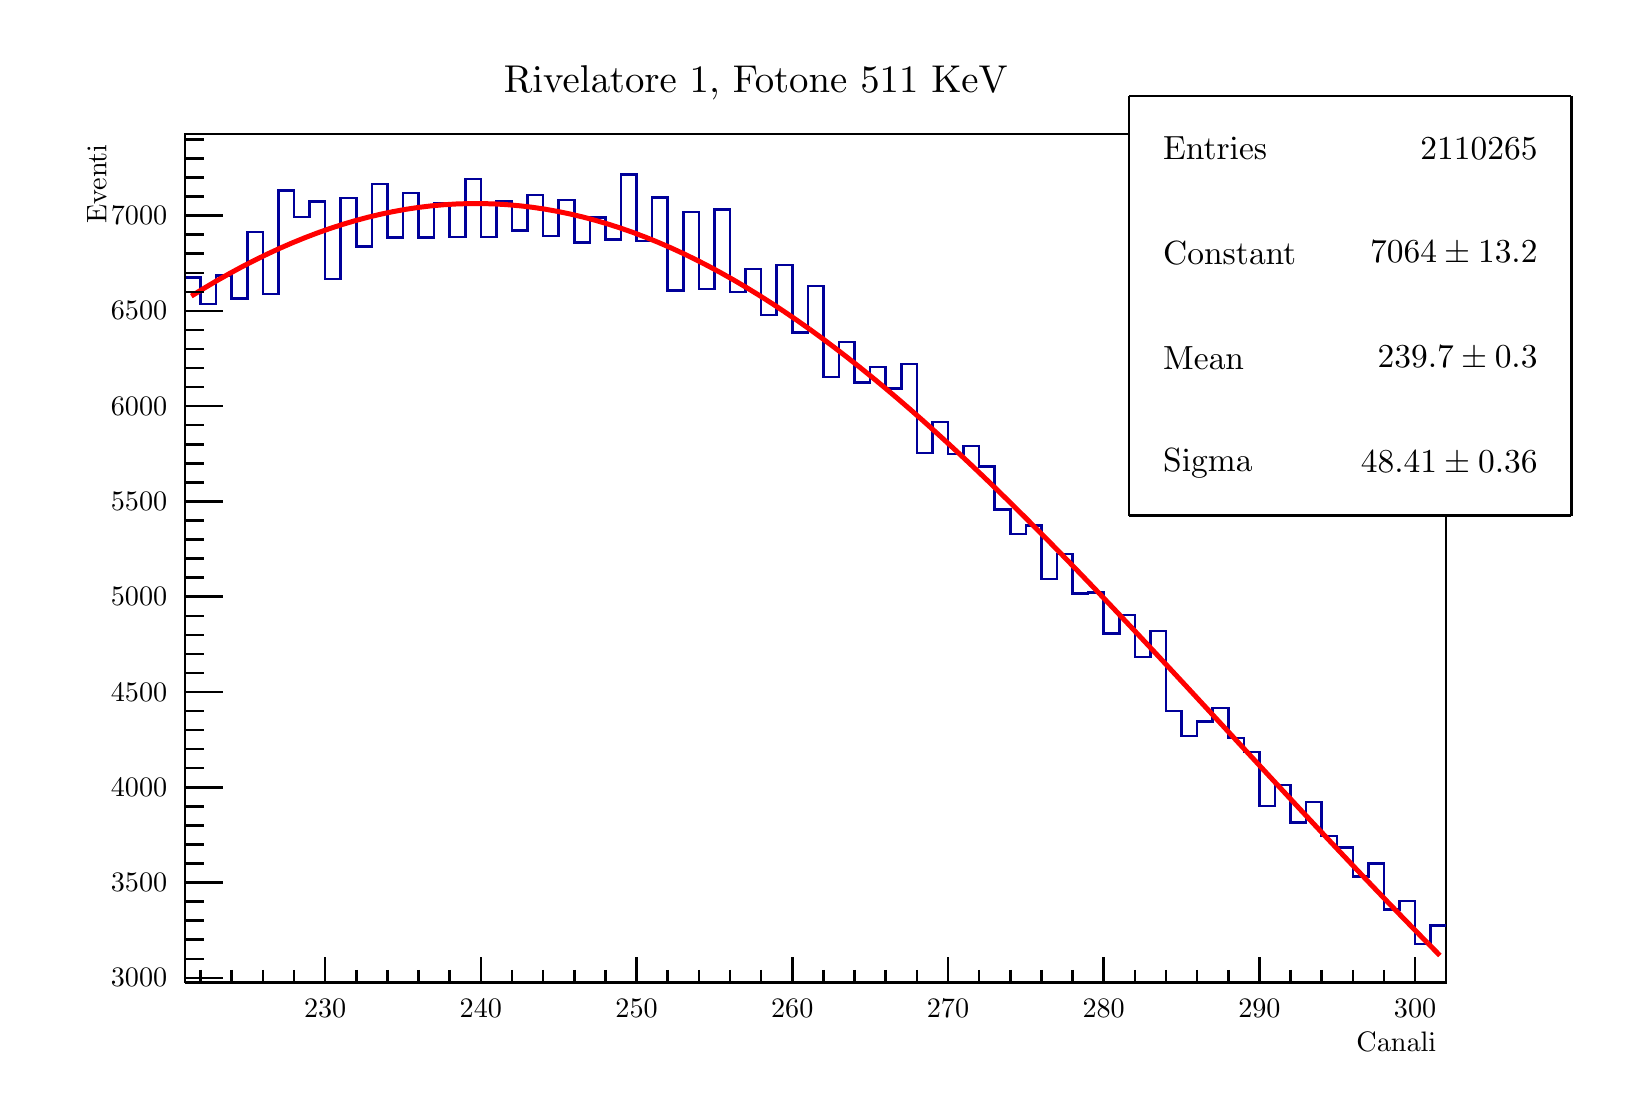
\begin{tikzpicture}
\pgfdeclareplotmark{cross} {
\pgfpathmoveto{\pgfpoint{-0.3\pgfplotmarksize}{\pgfplotmarksize}}
\pgfpathlineto{\pgfpoint{+0.3\pgfplotmarksize}{\pgfplotmarksize}}
\pgfpathlineto{\pgfpoint{+0.3\pgfplotmarksize}{0.3\pgfplotmarksize}}
\pgfpathlineto{\pgfpoint{+1\pgfplotmarksize}{0.3\pgfplotmarksize}}
\pgfpathlineto{\pgfpoint{+1\pgfplotmarksize}{-0.3\pgfplotmarksize}}
\pgfpathlineto{\pgfpoint{+0.3\pgfplotmarksize}{-0.3\pgfplotmarksize}}
\pgfpathlineto{\pgfpoint{+0.3\pgfplotmarksize}{-1.\pgfplotmarksize}}
\pgfpathlineto{\pgfpoint{-0.3\pgfplotmarksize}{-1.\pgfplotmarksize}}
\pgfpathlineto{\pgfpoint{-0.3\pgfplotmarksize}{-0.3\pgfplotmarksize}}
\pgfpathlineto{\pgfpoint{-1.\pgfplotmarksize}{-0.3\pgfplotmarksize}}
\pgfpathlineto{\pgfpoint{-1.\pgfplotmarksize}{0.3\pgfplotmarksize}}
\pgfpathlineto{\pgfpoint{-0.3\pgfplotmarksize}{0.3\pgfplotmarksize}}
\pgfpathclose
\pgfusepathqstroke
}
\pgfdeclareplotmark{cross*} {
\pgfpathmoveto{\pgfpoint{-0.3\pgfplotmarksize}{\pgfplotmarksize}}
\pgfpathlineto{\pgfpoint{+0.3\pgfplotmarksize}{\pgfplotmarksize}}
\pgfpathlineto{\pgfpoint{+0.3\pgfplotmarksize}{0.3\pgfplotmarksize}}
\pgfpathlineto{\pgfpoint{+1\pgfplotmarksize}{0.3\pgfplotmarksize}}
\pgfpathlineto{\pgfpoint{+1\pgfplotmarksize}{-0.3\pgfplotmarksize}}
\pgfpathlineto{\pgfpoint{+0.3\pgfplotmarksize}{-0.3\pgfplotmarksize}}
\pgfpathlineto{\pgfpoint{+0.3\pgfplotmarksize}{-1.\pgfplotmarksize}}
\pgfpathlineto{\pgfpoint{-0.3\pgfplotmarksize}{-1.\pgfplotmarksize}}
\pgfpathlineto{\pgfpoint{-0.3\pgfplotmarksize}{-0.3\pgfplotmarksize}}
\pgfpathlineto{\pgfpoint{-1.\pgfplotmarksize}{-0.3\pgfplotmarksize}}
\pgfpathlineto{\pgfpoint{-1.\pgfplotmarksize}{0.3\pgfplotmarksize}}
\pgfpathlineto{\pgfpoint{-0.3\pgfplotmarksize}{0.3\pgfplotmarksize}}
\pgfpathclose
\pgfusepathqfillstroke
}
\pgfdeclareplotmark{newstar} {
\pgfpathmoveto{\pgfqpoint{0pt}{\pgfplotmarksize}}
\pgfpathlineto{\pgfqpointpolar{44}{0.5\pgfplotmarksize}}
\pgfpathlineto{\pgfqpointpolar{18}{\pgfplotmarksize}}
\pgfpathlineto{\pgfqpointpolar{-20}{0.5\pgfplotmarksize}}
\pgfpathlineto{\pgfqpointpolar{-54}{\pgfplotmarksize}}
\pgfpathlineto{\pgfqpointpolar{-90}{0.5\pgfplotmarksize}}
\pgfpathlineto{\pgfqpointpolar{234}{\pgfplotmarksize}}
\pgfpathlineto{\pgfqpointpolar{198}{0.5\pgfplotmarksize}}
\pgfpathlineto{\pgfqpointpolar{162}{\pgfplotmarksize}}
\pgfpathlineto{\pgfqpointpolar{134}{0.5\pgfplotmarksize}}
\pgfpathclose
\pgfusepathqstroke
}
\pgfdeclareplotmark{newstar*} {
\pgfpathmoveto{\pgfqpoint{0pt}{\pgfplotmarksize}}
\pgfpathlineto{\pgfqpointpolar{44}{0.5\pgfplotmarksize}}
\pgfpathlineto{\pgfqpointpolar{18}{\pgfplotmarksize}}
\pgfpathlineto{\pgfqpointpolar{-20}{0.5\pgfplotmarksize}}
\pgfpathlineto{\pgfqpointpolar{-54}{\pgfplotmarksize}}
\pgfpathlineto{\pgfqpointpolar{-90}{0.5\pgfplotmarksize}}
\pgfpathlineto{\pgfqpointpolar{234}{\pgfplotmarksize}}
\pgfpathlineto{\pgfqpointpolar{198}{0.5\pgfplotmarksize}}
\pgfpathlineto{\pgfqpointpolar{162}{\pgfplotmarksize}}
\pgfpathlineto{\pgfqpointpolar{134}{0.5\pgfplotmarksize}}
\pgfpathclose
\pgfusepathqfillstroke
}
\definecolor{c}{rgb}{1,1,1};
\draw [color=c, fill=c] (0,0) rectangle (20,13.4957);
\draw [color=c, fill=c] (1.9914,1.37536) rectangle (18.0086,12.149);
\definecolor{c}{rgb}{0,0,0};
\draw [c,line width=0.9] (1.9914,1.37536) -- (1.9914,12.149) -- (18.0086,12.149) -- (18.0086,1.37536) -- (1.9914,1.37536);
\definecolor{c}{rgb}{1,1,1};
\draw [color=c, fill=c] (1.9914,1.37536) rectangle (18.0086,12.149);
\definecolor{c}{rgb}{0,0,0};
\draw [c,line width=0.9] (1.9914,1.37536) -- (1.9914,12.149) -- (18.0086,12.149) -- (18.0086,1.37536) -- (1.9914,1.37536);
\definecolor{c}{rgb}{0,0,0.6};
\draw [c,line width=0.9] (1.9914,10.3292) -- (2.18915,10.3292) -- (2.18915,9.99278) -- (2.38689,9.99278) -- (2.38689,10.3582) -- (2.58463,10.3582) -- (2.58463,10.063) -- (2.78238,10.063) -- (2.78238,10.91) -- (2.98012,10.91) -- (2.98012,10.1186) --
 (3.17786,10.1186) -- (3.17786,11.4327) -- (3.37561,11.4327) -- (3.37561,11.0987) -- (3.57335,11.0987) -- (3.57335,11.2947) -- (3.77109,11.2947) -- (3.77109,10.3122) -- (3.96884,10.3122) -- (3.96884,11.3383) -- (4.16658,11.3383) -- (4.16658,10.7236)
 -- (4.36432,10.7236) -- (4.36432,11.515) -- (4.56206,11.515) -- (4.56206,10.8398) -- (4.75981,10.8398) -- (4.75981,11.4036) -- (4.95755,11.4036) -- (4.95755,10.8374) -- (5.15529,10.8374) -- (5.15529,11.2705) -- (5.35304,11.2705) -- (5.35304,10.8422)
 -- (5.55078,10.8422) -- (5.55078,11.5827) -- (5.74852,11.5827) -- (5.74852,10.8446) -- (5.94627,10.8446) -- (5.94627,11.2972) -- (6.14401,11.2972) -- (6.14401,10.9269) -- (6.34175,10.9269) -- (6.34175,11.3794) -- (6.5395,11.3794) -- (6.5395,10.8567)
 -- (6.73724,10.8567) -- (6.73724,11.3141) -- (6.93498,11.3141) -- (6.93498,10.772) -- (7.13272,10.772) -- (7.13272,11.0915) -- (7.33047,11.0915) -- (7.33047,10.8132) -- (7.52821,10.8132) -- (7.52821,11.636) -- (7.72595,11.636) -- (7.72595,10.7914)
 -- (7.9237,10.7914) -- (7.9237,11.348) -- (8.12144,11.348) -- (8.12144,10.1646) -- (8.31918,10.1646) -- (8.31918,11.1616) -- (8.51693,11.1616) -- (8.51693,10.184) -- (8.71467,10.184) -- (8.71467,11.1907) -- (8.91241,11.1907) -- (8.91241,10.1452) --
 (9.11016,10.1452) -- (9.11016,10.4381) -- (9.3079,10.4381) -- (9.3079,9.85484) -- (9.50564,9.85484) -- (9.50564,10.4865) -- (9.70339,10.4865) -- (9.70339,9.62978) -- (9.90113,9.62978) -- (9.90113,10.2227) -- (10.0989,10.2227) -- (10.0989,9.06833) --
 (10.2966,9.06833) -- (10.2966,9.5112) -- (10.4944,9.5112) -- (10.4944,8.99331) -- (10.6921,8.99331) -- (10.6921,9.19417) -- (10.8898,9.19417) -- (10.8898,8.92313) -- (11.0876,8.92313) -- (11.0876,9.23289) -- (11.2853,9.23289) -- (11.2853,8.10033) --
 (11.4831,8.10033) -- (11.4831,8.49479) -- (11.6808,8.49479) -- (11.6808,8.08581) -- (11.8786,8.08581) -- (11.8786,8.19229) -- (12.0763,8.19229) -- (12.0763,7.93093) -- (12.274,7.93093) -- (12.274,7.38159) -- (12.4718,7.38159) -- (12.4718,7.07182) --
 (12.6695,7.07182) -- (12.6695,7.1783) -- (12.8673,7.1783) -- (12.8673,6.5007) -- (13.065,6.5007) -- (13.065,6.81772) -- (13.2628,6.81772) -- (13.2628,6.3192) -- (13.4605,6.3192) -- (13.4605,6.32646) -- (13.6582,6.32646) -- (13.6582,5.811) --
 (13.856,5.811) -- (13.856,6.04332) -- (14.0537,6.04332) -- (14.0537,5.5085) -- (14.2515,5.5085) -- (14.2515,5.83762) -- (14.4492,5.83762) -- (14.4492,4.82605) -- (14.647,4.82605) -- (14.647,4.50903) -- (14.8447,4.50903) -- (14.8447,4.69295) --
 (15.0424,4.69295) -- (15.0424,4.85993) -- (15.2402,4.85993) -- (15.2402,4.48241) -- (15.4379,4.48241) -- (15.4379,4.30091) -- (15.6357,4.30091) -- (15.6357,3.61847) -- (15.8334,3.61847) -- (15.8334,3.88467) -- (16.0312,3.88467) -- (16.0312,3.40793)
 -- (16.2289,3.40793) -- (16.2289,3.67171) -- (16.4267,3.67171) -- (16.4267,3.23853) -- (16.6244,3.23853) -- (16.6244,3.09332) -- (16.8221,3.09332) -- (16.8221,2.72064) -- (17.0199,2.72064) -- (17.0199,2.88762) -- (17.2176,2.88762) --
 (17.2176,2.3044) -- (17.4154,2.3044) -- (17.4154,2.41088) -- (17.6131,2.41088) -- (17.6131,1.86396) -- (17.8109,1.86396) -- (17.8109,2.0987) -- (18.0086,2.0987);
\definecolor{c}{rgb}{1,1,1};
\draw [color=c, fill=c] (13.9828,7.30659) rectangle (19.5989,12.6361);
\definecolor{c}{rgb}{0,0,0};
\draw [c,line width=0.9] (13.9828,7.30659) -- (19.5989,7.30659);
\draw [c,line width=0.9] (19.5989,7.30659) -- (19.5989,12.6361);
\draw [c,line width=0.9] (19.5989,12.6361) -- (13.9828,12.6361);
\draw [c,line width=0.9] (13.9828,12.6361) -- (13.9828,7.30659);
\draw [anchor= west] (14.2636,11.9699) node[scale=1.20912, color=c, rotate=0]{Entries };
\draw [anchor= east] (19.3181,11.9699) node[scale=1.20912, color=c, rotate=0]{ 2110265};
\draw [anchor= west] (14.2636,10.6375) node[scale=1.20912, color=c, rotate=0]{Constant };
\draw [anchor= east] (19.3181,10.6375) node[scale=1.20912, color=c, rotate=0]{$  7064 \pm 13.2$};
\draw [anchor= west] (14.2636,9.30516) node[scale=1.20912, color=c, rotate=0]{Mean     };
\draw [anchor= east] (19.3181,9.30516) node[scale=1.20912, color=c, rotate=0]{$ 239.7 \pm 0.3$};
\draw [anchor= west] (14.2636,7.97278) node[scale=1.20912, color=c, rotate=0]{Sigma    };
\draw [anchor= east] (19.3181,7.97278) node[scale=1.20912, color=c, rotate=0]{$ 48.41 \pm 0.36$};
\definecolor{c}{rgb}{1,0,0};
\draw [c,line width=1.8] (2.07149,10.0938) -- (2.23166,10.1924) -- (2.39183,10.2871) -- (2.55201,10.3779) -- (2.71218,10.4646) -- (2.87235,10.5471) -- (3.03252,10.6255) -- (3.19269,10.6997) -- (3.35287,10.7695) -- (3.51304,10.8349) --
 (3.67321,10.896) -- (3.83338,10.9525) -- (3.99355,11.0046) -- (4.15373,11.052) -- (4.3139,11.0949) -- (4.47407,11.1331) -- (4.63424,11.1667) -- (4.79441,11.1955) -- (4.95458,11.2197) -- (5.11476,11.2391) -- (5.27493,11.2537) -- (5.4351,11.2635) --
 (5.59527,11.2686) -- (5.75544,11.2689) -- (5.91562,11.2644) -- (6.07579,11.2551) -- (6.23596,11.2411) -- (6.39613,11.2223) -- (6.5563,11.1987) -- (6.71648,11.1704) -- (6.87665,11.1374) -- (7.03682,11.0998) -- (7.19699,11.0575) -- (7.35716,11.0105)
 -- (7.51734,10.9591) -- (7.67751,10.903) -- (7.83768,10.8425) -- (7.99785,10.7776) -- (8.15802,10.7083) -- (8.31819,10.6347) -- (8.47837,10.5568) -- (8.63854,10.4747) -- (8.79871,10.3885) -- (8.95888,10.2983) -- (9.11905,10.204) -- (9.27923,10.1059)
 -- (9.4394,10.0039) -- (9.59957,9.89814) -- (9.75974,9.78874) -- (9.91991,9.67575);
\draw [c,line width=1.8] (9.91991,9.67575) -- (10.0801,9.55928) -- (10.2403,9.4394) -- (10.4004,9.31623) -- (10.5606,9.18983) -- (10.7208,9.06033) -- (10.8809,8.92781) -- (11.0411,8.79238) -- (11.2013,8.65414) -- (11.3615,8.51319) --
 (11.5216,8.36964) -- (11.6818,8.22359) -- (11.842,8.07516) -- (12.0021,7.92444) -- (12.1623,7.77154) -- (12.3225,7.61659) -- (12.4827,7.45968) -- (12.6428,7.30092) -- (12.803,7.14044) -- (12.9632,6.97833) -- (13.1234,6.8147) -- (13.2835,6.64968) --
 (13.4437,6.48336) -- (13.6039,6.31587) -- (13.764,6.1473) -- (13.9242,5.97776) -- (14.0844,5.80737) -- (14.2446,5.63623) -- (14.4047,5.46444) -- (14.5649,5.29212) -- (14.7251,5.11936) -- (14.8852,4.94628) -- (15.0454,4.77296) -- (15.2056,4.59951) --
 (15.3658,4.42603) -- (15.5259,4.25262) -- (15.6861,4.07936) -- (15.8463,3.90636) -- (16.0064,3.73371) -- (16.1666,3.56149) -- (16.3268,3.38979) -- (16.487,3.21871) -- (16.6471,3.04831) -- (16.8073,2.87869) -- (16.9675,2.70992) -- (17.1277,2.54208)
 -- (17.2878,2.37524) -- (17.448,2.20949) -- (17.6082,2.04488) -- (17.7683,1.88148);
\draw [c,line width=1.8] (17.7683,1.88148) -- (17.9285,1.71937);
\definecolor{c}{rgb}{0,0,0};
\draw [c,line width=0.9] (1.9914,1.37536) -- (18.0086,1.37536);
\draw [anchor= east] (18.0086,0.619599) node[scale=1.01821, color=c, rotate=0]{Canali};
\draw [c,line width=0.9] (3.77109,1.6996) -- (3.77109,1.37536);
\draw [c,line width=0.9] (4.16658,1.53748) -- (4.16658,1.37536);
\draw [c,line width=0.9] (4.56206,1.53748) -- (4.56206,1.37536);
\draw [c,line width=0.9] (4.95755,1.53748) -- (4.95755,1.37536);
\draw [c,line width=0.9] (5.35304,1.53748) -- (5.35304,1.37536);
\draw [c,line width=0.9] (5.74852,1.6996) -- (5.74852,1.37536);
\draw [c,line width=0.9] (6.14401,1.53748) -- (6.14401,1.37536);
\draw [c,line width=0.9] (6.5395,1.53748) -- (6.5395,1.37536);
\draw [c,line width=0.9] (6.93498,1.53748) -- (6.93498,1.37536);
\draw [c,line width=0.9] (7.33047,1.53748) -- (7.33047,1.37536);
\draw [c,line width=0.9] (7.72595,1.6996) -- (7.72595,1.37536);
\draw [c,line width=0.9] (8.12144,1.53748) -- (8.12144,1.37536);
\draw [c,line width=0.9] (8.51693,1.53748) -- (8.51693,1.37536);
\draw [c,line width=0.9] (8.91241,1.53748) -- (8.91241,1.37536);
\draw [c,line width=0.9] (9.3079,1.53748) -- (9.3079,1.37536);
\draw [c,line width=0.9] (9.70339,1.6996) -- (9.70339,1.37536);
\draw [c,line width=0.9] (10.0989,1.53748) -- (10.0989,1.37536);
\draw [c,line width=0.9] (10.4944,1.53748) -- (10.4944,1.37536);
\draw [c,line width=0.9] (10.8898,1.53748) -- (10.8898,1.37536);
\draw [c,line width=0.9] (11.2853,1.53748) -- (11.2853,1.37536);
\draw [c,line width=0.9] (11.6808,1.6996) -- (11.6808,1.37536);
\draw [c,line width=0.9] (12.0763,1.53748) -- (12.0763,1.37536);
\draw [c,line width=0.9] (12.4718,1.53748) -- (12.4718,1.37536);
\draw [c,line width=0.9] (12.8673,1.53748) -- (12.8673,1.37536);
\draw [c,line width=0.9] (13.2628,1.53748) -- (13.2628,1.37536);
\draw [c,line width=0.9] (13.6582,1.6996) -- (13.6582,1.37536);
\draw [c,line width=0.9] (14.0537,1.53748) -- (14.0537,1.37536);
\draw [c,line width=0.9] (14.4492,1.53748) -- (14.4492,1.37536);
\draw [c,line width=0.9] (14.8447,1.53748) -- (14.8447,1.37536);
\draw [c,line width=0.9] (15.2402,1.53748) -- (15.2402,1.37536);
\draw [c,line width=0.9] (15.6357,1.6996) -- (15.6357,1.37536);
\draw [c,line width=0.9] (16.0312,1.53748) -- (16.0312,1.37536);
\draw [c,line width=0.9] (16.4267,1.53748) -- (16.4267,1.37536);
\draw [c,line width=0.9] (16.8221,1.53748) -- (16.8221,1.37536);
\draw [c,line width=0.9] (17.2176,1.53748) -- (17.2176,1.37536);
\draw [c,line width=0.9] (17.6131,1.6996) -- (17.6131,1.37536);
\draw [c,line width=0.9] (3.77109,1.6996) -- (3.77109,1.37536);
\draw [c,line width=0.9] (3.37561,1.53748) -- (3.37561,1.37536);
\draw [c,line width=0.9] (2.98012,1.53748) -- (2.98012,1.37536);
\draw [c,line width=0.9] (2.58463,1.53748) -- (2.58463,1.37536);
\draw [c,line width=0.9] (2.18915,1.53748) -- (2.18915,1.37536);
\draw [c,line width=0.9] (17.6131,1.6996) -- (17.6131,1.37536);
\draw [c,line width=0.9] (18.0086,1.53748) -- (18.0086,1.37536);
\draw [anchor=base] (3.77109,0.93) node[scale=1.01821, color=c, rotate=0]{230};
\draw [anchor=base] (5.74852,0.93) node[scale=1.01821, color=c, rotate=0]{240};
\draw [anchor=base] (7.72595,0.93) node[scale=1.01821, color=c, rotate=0]{250};
\draw [anchor=base] (9.70339,0.93) node[scale=1.01821, color=c, rotate=0]{260};
\draw [anchor=base] (11.6808,0.93) node[scale=1.01821, color=c, rotate=0]{270};
\draw [anchor=base] (13.6582,0.93) node[scale=1.01821, color=c, rotate=0]{280};
\draw [anchor=base] (15.6357,0.93) node[scale=1.01821, color=c, rotate=0]{290};
\draw [anchor=base] (17.6131,0.93) node[scale=1.01821, color=c, rotate=0]{300};
\draw [c,line width=0.9] (1.9914,1.37536) -- (1.9914,12.149);
\draw [anchor= east] (0.871404,12.149) node[scale=1.01821, color=c, rotate=90]{Eventi};
\draw [c,line width=0.9] (2.47038,1.43562) -- (1.9914,1.43562);
\draw [c,line width=0.9] (2.23089,1.67762) -- (1.9914,1.67762);
\draw [c,line width=0.9] (2.23089,1.91962) -- (1.9914,1.91962);
\draw [c,line width=0.9] (2.23089,2.16162) -- (1.9914,2.16162);
\draw [c,line width=0.9] (2.23089,2.40362) -- (1.9914,2.40362);
\draw [c,line width=0.9] (2.47038,2.64562) -- (1.9914,2.64562);
\draw [c,line width=0.9] (2.23089,2.88762) -- (1.9914,2.88762);
\draw [c,line width=0.9] (2.23089,3.12962) -- (1.9914,3.12962);
\draw [c,line width=0.9] (2.23089,3.37163) -- (1.9914,3.37163);
\draw [c,line width=0.9] (2.23089,3.61363) -- (1.9914,3.61363);
\draw [c,line width=0.9] (2.47038,3.85563) -- (1.9914,3.85563);
\draw [c,line width=0.9] (2.23089,4.09763) -- (1.9914,4.09763);
\draw [c,line width=0.9] (2.23089,4.33963) -- (1.9914,4.33963);
\draw [c,line width=0.9] (2.23089,4.58163) -- (1.9914,4.58163);
\draw [c,line width=0.9] (2.23089,4.82363) -- (1.9914,4.82363);
\draw [c,line width=0.9] (2.47038,5.06563) -- (1.9914,5.06563);
\draw [c,line width=0.9] (2.23089,5.30764) -- (1.9914,5.30764);
\draw [c,line width=0.9] (2.23089,5.54964) -- (1.9914,5.54964);
\draw [c,line width=0.9] (2.23089,5.79164) -- (1.9914,5.79164);
\draw [c,line width=0.9] (2.23089,6.03364) -- (1.9914,6.03364);
\draw [c,line width=0.9] (2.47038,6.27564) -- (1.9914,6.27564);
\draw [c,line width=0.9] (2.23089,6.51764) -- (1.9914,6.51764);
\draw [c,line width=0.9] (2.23089,6.75964) -- (1.9914,6.75964);
\draw [c,line width=0.9] (2.23089,7.00164) -- (1.9914,7.00164);
\draw [c,line width=0.9] (2.23089,7.24365) -- (1.9914,7.24365);
\draw [c,line width=0.9] (2.47038,7.48565) -- (1.9914,7.48565);
\draw [c,line width=0.9] (2.23089,7.72765) -- (1.9914,7.72765);
\draw [c,line width=0.9] (2.23089,7.96965) -- (1.9914,7.96965);
\draw [c,line width=0.9] (2.23089,8.21165) -- (1.9914,8.21165);
\draw [c,line width=0.9] (2.23089,8.45365) -- (1.9914,8.45365);
\draw [c,line width=0.9] (2.47038,8.69565) -- (1.9914,8.69565);
\draw [c,line width=0.9] (2.23089,8.93765) -- (1.9914,8.93765);
\draw [c,line width=0.9] (2.23089,9.17965) -- (1.9914,9.17965);
\draw [c,line width=0.9] (2.23089,9.42166) -- (1.9914,9.42166);
\draw [c,line width=0.9] (2.23089,9.66366) -- (1.9914,9.66366);
\draw [c,line width=0.9] (2.47038,9.90566) -- (1.9914,9.90566);
\draw [c,line width=0.9] (2.23089,10.1477) -- (1.9914,10.1477);
\draw [c,line width=0.9] (2.23089,10.3897) -- (1.9914,10.3897);
\draw [c,line width=0.9] (2.23089,10.6317) -- (1.9914,10.6317);
\draw [c,line width=0.9] (2.23089,10.8737) -- (1.9914,10.8737);
\draw [c,line width=0.9] (2.47038,11.1157) -- (1.9914,11.1157);
\draw [c,line width=0.9] (2.47038,1.43562) -- (1.9914,1.43562);
\draw [c,line width=0.9] (2.47038,11.1157) -- (1.9914,11.1157);
\draw [c,line width=0.9] (2.23089,11.3577) -- (1.9914,11.3577);
\draw [c,line width=0.9] (2.23089,11.5997) -- (1.9914,11.5997);
\draw [c,line width=0.9] (2.23089,11.8417) -- (1.9914,11.8417);
\draw [c,line width=0.9] (2.23089,12.0837) -- (1.9914,12.0837);
\draw [anchor= east] (1.8914,1.43562) node[scale=1.01821, color=c, rotate=0]{3000};
\draw [anchor= east] (1.8914,2.64562) node[scale=1.01821, color=c, rotate=0]{3500};
\draw [anchor= east] (1.8914,3.85563) node[scale=1.01821, color=c, rotate=0]{4000};
\draw [anchor= east] (1.8914,5.06563) node[scale=1.01821, color=c, rotate=0]{4500};
\draw [anchor= east] (1.8914,6.27564) node[scale=1.01821, color=c, rotate=0]{5000};
\draw [anchor= east] (1.8914,7.48565) node[scale=1.01821, color=c, rotate=0]{5500};
\draw [anchor= east] (1.8914,8.69565) node[scale=1.01821, color=c, rotate=0]{6000};
\draw [anchor= east] (1.8914,9.90566) node[scale=1.01821, color=c, rotate=0]{6500};
\draw [anchor= east] (1.8914,11.1157) node[scale=1.01821, color=c, rotate=0]{7000};
\definecolor{c}{rgb}{1,1,1};
\draw [color=c, fill=c] (13.9828,7.30659) rectangle (19.5989,12.6361);
\definecolor{c}{rgb}{0,0,0};
\draw [c,line width=0.9] (13.9828,7.30659) -- (19.5989,7.30659);
\draw [c,line width=0.9] (19.5989,7.30659) -- (19.5989,12.6361);
\draw [c,line width=0.9] (19.5989,12.6361) -- (13.9828,12.6361);
\draw [c,line width=0.9] (13.9828,12.6361) -- (13.9828,7.30659);
\draw [anchor= west] (14.2636,11.9699) node[scale=1.20912, color=c, rotate=0]{Entries };
\draw [anchor= east] (19.3181,11.9699) node[scale=1.20912, color=c, rotate=0]{ 2110265};
\draw [anchor= west] (14.2636,10.6375) node[scale=1.20912, color=c, rotate=0]{Constant };
\draw [anchor= east] (19.3181,10.6375) node[scale=1.20912, color=c, rotate=0]{$  7064 \pm 13.2$};
\draw [anchor= west] (14.2636,9.30516) node[scale=1.20912, color=c, rotate=0]{Mean     };
\draw [anchor= east] (19.3181,9.30516) node[scale=1.20912, color=c, rotate=0]{$ 239.7 \pm 0.3$};
\draw [anchor= west] (14.2636,7.97278) node[scale=1.20912, color=c, rotate=0]{Sigma    };
\draw [anchor= east] (19.3181,7.97278) node[scale=1.20912, color=c, rotate=0]{$ 48.41 \pm 0.36$};
\draw (9.24069,12.808) node[scale=1.40004, color=c, rotate=0]{Rivelatore 1, Fotone 511 KeV};
\end{tikzpicture}

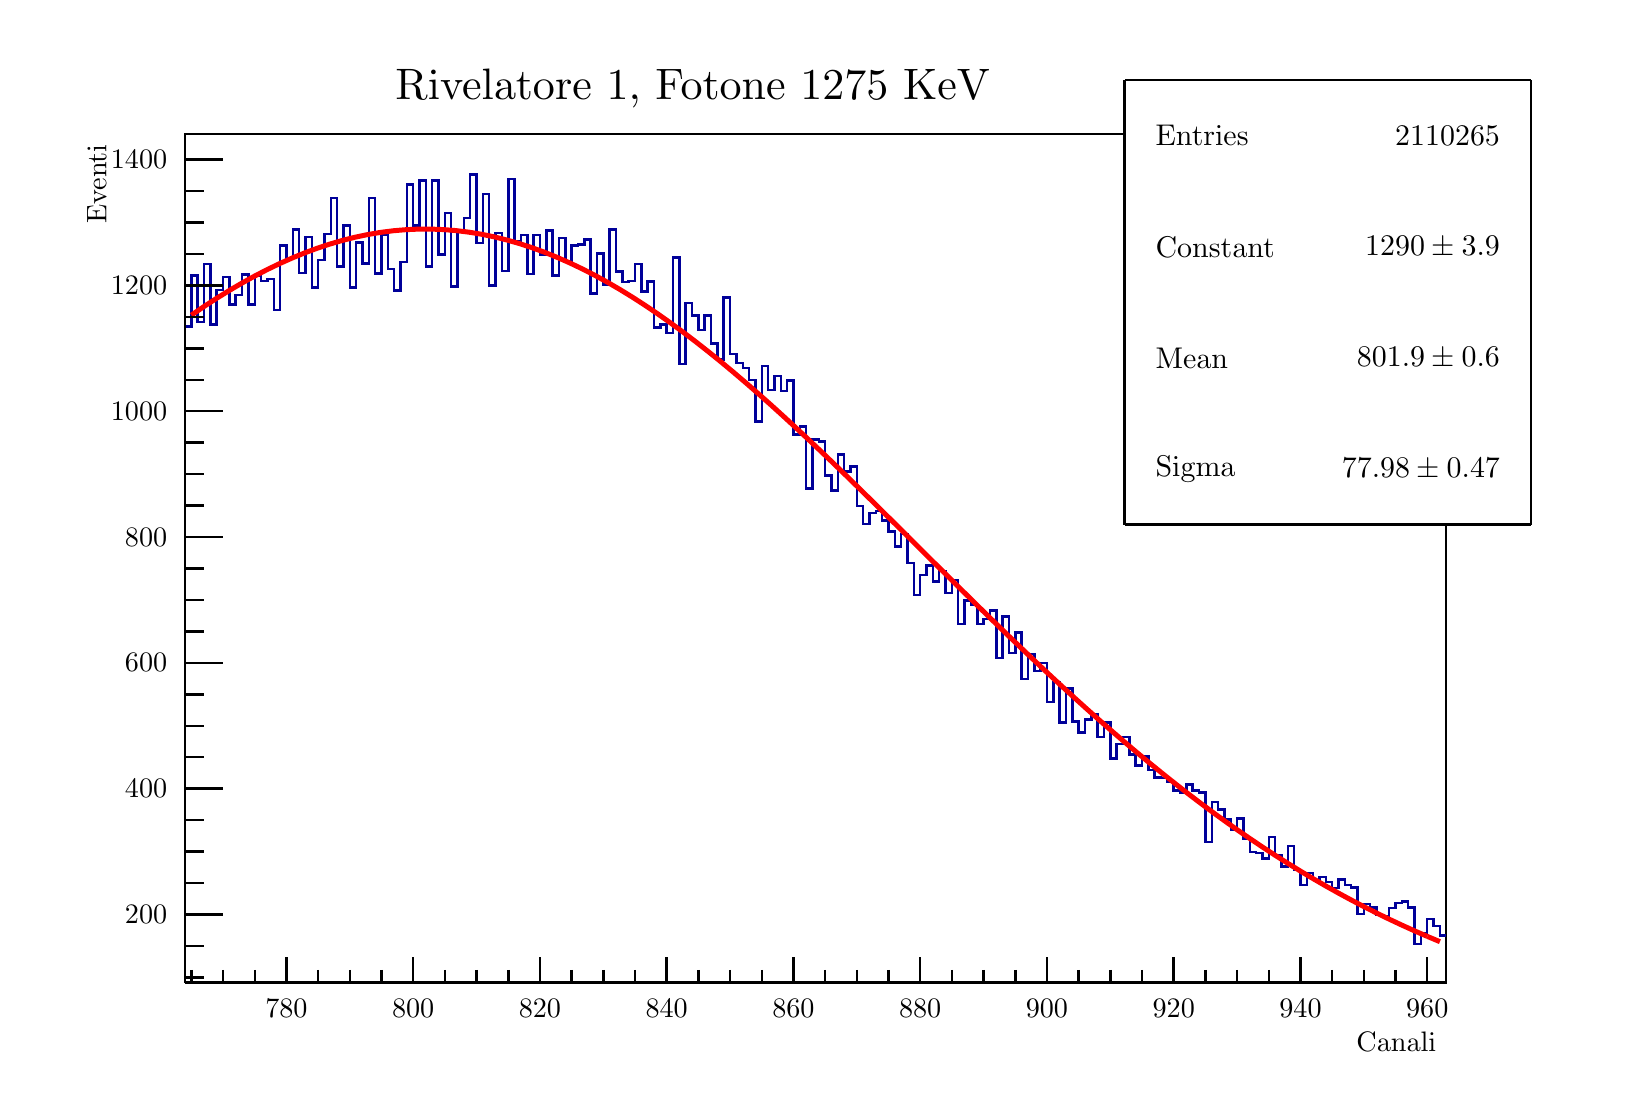
\begin{tikzpicture}
\pgfdeclareplotmark{cross} {
\pgfpathmoveto{\pgfpoint{-0.3\pgfplotmarksize}{\pgfplotmarksize}}
\pgfpathlineto{\pgfpoint{+0.3\pgfplotmarksize}{\pgfplotmarksize}}
\pgfpathlineto{\pgfpoint{+0.3\pgfplotmarksize}{0.3\pgfplotmarksize}}
\pgfpathlineto{\pgfpoint{+1\pgfplotmarksize}{0.3\pgfplotmarksize}}
\pgfpathlineto{\pgfpoint{+1\pgfplotmarksize}{-0.3\pgfplotmarksize}}
\pgfpathlineto{\pgfpoint{+0.3\pgfplotmarksize}{-0.3\pgfplotmarksize}}
\pgfpathlineto{\pgfpoint{+0.3\pgfplotmarksize}{-1.\pgfplotmarksize}}
\pgfpathlineto{\pgfpoint{-0.3\pgfplotmarksize}{-1.\pgfplotmarksize}}
\pgfpathlineto{\pgfpoint{-0.3\pgfplotmarksize}{-0.3\pgfplotmarksize}}
\pgfpathlineto{\pgfpoint{-1.\pgfplotmarksize}{-0.3\pgfplotmarksize}}
\pgfpathlineto{\pgfpoint{-1.\pgfplotmarksize}{0.3\pgfplotmarksize}}
\pgfpathlineto{\pgfpoint{-0.3\pgfplotmarksize}{0.3\pgfplotmarksize}}
\pgfpathclose
\pgfusepathqstroke
}
\pgfdeclareplotmark{cross*} {
\pgfpathmoveto{\pgfpoint{-0.3\pgfplotmarksize}{\pgfplotmarksize}}
\pgfpathlineto{\pgfpoint{+0.3\pgfplotmarksize}{\pgfplotmarksize}}
\pgfpathlineto{\pgfpoint{+0.3\pgfplotmarksize}{0.3\pgfplotmarksize}}
\pgfpathlineto{\pgfpoint{+1\pgfplotmarksize}{0.3\pgfplotmarksize}}
\pgfpathlineto{\pgfpoint{+1\pgfplotmarksize}{-0.3\pgfplotmarksize}}
\pgfpathlineto{\pgfpoint{+0.3\pgfplotmarksize}{-0.3\pgfplotmarksize}}
\pgfpathlineto{\pgfpoint{+0.3\pgfplotmarksize}{-1.\pgfplotmarksize}}
\pgfpathlineto{\pgfpoint{-0.3\pgfplotmarksize}{-1.\pgfplotmarksize}}
\pgfpathlineto{\pgfpoint{-0.3\pgfplotmarksize}{-0.3\pgfplotmarksize}}
\pgfpathlineto{\pgfpoint{-1.\pgfplotmarksize}{-0.3\pgfplotmarksize}}
\pgfpathlineto{\pgfpoint{-1.\pgfplotmarksize}{0.3\pgfplotmarksize}}
\pgfpathlineto{\pgfpoint{-0.3\pgfplotmarksize}{0.3\pgfplotmarksize}}
\pgfpathclose
\pgfusepathqfillstroke
}
\pgfdeclareplotmark{newstar} {
\pgfpathmoveto{\pgfqpoint{0pt}{\pgfplotmarksize}}
\pgfpathlineto{\pgfqpointpolar{44}{0.5\pgfplotmarksize}}
\pgfpathlineto{\pgfqpointpolar{18}{\pgfplotmarksize}}
\pgfpathlineto{\pgfqpointpolar{-20}{0.5\pgfplotmarksize}}
\pgfpathlineto{\pgfqpointpolar{-54}{\pgfplotmarksize}}
\pgfpathlineto{\pgfqpointpolar{-90}{0.5\pgfplotmarksize}}
\pgfpathlineto{\pgfqpointpolar{234}{\pgfplotmarksize}}
\pgfpathlineto{\pgfqpointpolar{198}{0.5\pgfplotmarksize}}
\pgfpathlineto{\pgfqpointpolar{162}{\pgfplotmarksize}}
\pgfpathlineto{\pgfqpointpolar{134}{0.5\pgfplotmarksize}}
\pgfpathclose
\pgfusepathqstroke
}
\pgfdeclareplotmark{newstar*} {
\pgfpathmoveto{\pgfqpoint{0pt}{\pgfplotmarksize}}
\pgfpathlineto{\pgfqpointpolar{44}{0.5\pgfplotmarksize}}
\pgfpathlineto{\pgfqpointpolar{18}{\pgfplotmarksize}}
\pgfpathlineto{\pgfqpointpolar{-20}{0.5\pgfplotmarksize}}
\pgfpathlineto{\pgfqpointpolar{-54}{\pgfplotmarksize}}
\pgfpathlineto{\pgfqpointpolar{-90}{0.5\pgfplotmarksize}}
\pgfpathlineto{\pgfqpointpolar{234}{\pgfplotmarksize}}
\pgfpathlineto{\pgfqpointpolar{198}{0.5\pgfplotmarksize}}
\pgfpathlineto{\pgfqpointpolar{162}{\pgfplotmarksize}}
\pgfpathlineto{\pgfqpointpolar{134}{0.5\pgfplotmarksize}}
\pgfpathclose
\pgfusepathqfillstroke
}
\definecolor{c}{rgb}{1,1,1};
\draw [color=c, fill=c] (0,0) rectangle (20,13.4957);
\draw [color=c, fill=c] (1.9914,1.37536) rectangle (18.0086,12.149);
\definecolor{c}{rgb}{0,0,0};
\draw [c,line width=0.9] (1.9914,1.37536) -- (1.9914,12.149) -- (18.0086,12.149) -- (18.0086,1.37536) -- (1.9914,1.37536);
\definecolor{c}{rgb}{1,1,1};
\draw [color=c, fill=c] (1.9914,1.37536) rectangle (18.0086,12.149);
\definecolor{c}{rgb}{0,0,0};
\draw [c,line width=0.9] (1.9914,1.37536) -- (1.9914,12.149) -- (18.0086,12.149) -- (18.0086,1.37536) -- (1.9914,1.37536);
\definecolor{c}{rgb}{0,0,0.6};
\draw [c,line width=0.9] (1.9914,9.71033) -- (2.07189,9.71033) -- (2.07189,10.3575) -- (2.15238,10.3575) -- (2.15238,9.76626) -- (2.23287,9.76626) -- (2.23287,10.5014) -- (2.31336,10.5014) -- (2.31336,9.7343) -- (2.39385,9.7343) -- (2.39385,10.1738)
 -- (2.47433,10.1738) -- (2.47433,10.3336) -- (2.55482,10.3336) -- (2.55482,9.98999) -- (2.63531,9.98999) -- (2.63531,10.1098) -- (2.7158,10.1098) -- (2.7158,10.3655) -- (2.79629,10.3655) -- (2.79629,9.98999) -- (2.87678,9.98999) -- (2.87678,10.3575)
 -- (2.95726,10.3575) -- (2.95726,10.2856) -- (3.03775,10.2856) -- (3.03775,10.3096) -- (3.11824,10.3096) -- (3.11824,9.91807) -- (3.19873,9.91807) -- (3.19873,10.7331) -- (3.27922,10.7331) -- (3.27922,10.5733) -- (3.35971,10.5733) --
 (3.35971,10.9408) -- (3.4402,10.9408) -- (3.4402,10.3895) -- (3.52068,10.3895) -- (3.52068,10.8449) -- (3.60117,10.8449) -- (3.60117,10.2057) -- (3.68166,10.2057) -- (3.68166,10.5493) -- (3.76215,10.5493) -- (3.76215,10.8849) -- (3.84264,10.8849) --
 (3.84264,11.3403) -- (3.92313,11.3403) -- (3.92313,10.4694) -- (4.00361,10.4694) -- (4.00361,10.9888) -- (4.0841,10.9888) -- (4.0841,10.2057) -- (4.16459,10.2057) -- (4.16459,10.773) -- (4.24508,10.773) -- (4.24508,10.5093) -- (4.32557,10.5093) --
 (4.32557,11.3403) -- (4.40606,11.3403) -- (4.40606,10.3815) -- (4.48654,10.3815) -- (4.48654,10.8769) -- (4.56703,10.8769) -- (4.56703,10.4374) -- (4.64752,10.4374) -- (4.64752,10.1658) -- (4.72801,10.1658) -- (4.72801,10.5253) -- (4.8085,10.5253)
 -- (4.8085,11.5081) -- (4.88899,11.5081) -- (4.88899,10.9888) -- (4.96947,10.9888) -- (4.96947,11.5641) -- (5.04996,11.5641) -- (5.04996,10.4694) -- (5.13045,10.4694) -- (5.13045,11.5641) -- (5.21094,11.5641) -- (5.21094,10.6212) --
 (5.29143,10.6212) -- (5.29143,11.1486) -- (5.37192,11.1486) -- (5.37192,10.2137) -- (5.45241,10.2137) -- (5.45241,10.9168) -- (5.53289,10.9168) -- (5.53289,11.0846) -- (5.61338,11.0846) -- (5.61338,11.636) -- (5.69387,11.636) -- (5.69387,10.765) --
 (5.77436,10.765) -- (5.77436,11.3883) -- (5.85485,11.3883) -- (5.85485,10.2297) -- (5.93534,10.2297) -- (5.93534,10.8929) -- (6.01582,10.8929) -- (6.01582,10.4135) -- (6.09631,10.4135) -- (6.09631,11.58) -- (6.1768,11.58) -- (6.1768,10.789) --
 (6.25729,10.789) -- (6.25729,10.8689) -- (6.33778,10.8689) -- (6.33778,10.3735) -- (6.41827,10.3735) -- (6.41827,10.8689) -- (6.49875,10.8689) -- (6.49875,10.6212) -- (6.57924,10.6212) -- (6.57924,10.9248) -- (6.65973,10.9248) -- (6.65973,10.3575)
 -- (6.74022,10.3575) -- (6.74022,10.829) -- (6.82071,10.829) -- (6.82071,10.5253) -- (6.9012,10.5253) -- (6.9012,10.7331) -- (6.98169,10.7331) -- (6.98169,10.7491) -- (7.06217,10.7491) -- (7.06217,10.813) -- (7.14266,10.813) -- (7.14266,10.1258) --
 (7.22315,10.1258) -- (7.22315,10.6372) -- (7.30364,10.6372) -- (7.30364,10.2377) -- (7.38413,10.2377) -- (7.38413,10.9408) -- (7.46462,10.9408) -- (7.46462,10.4055) -- (7.5451,10.4055) -- (7.5451,10.2696) -- (7.62559,10.2696) -- (7.62559,10.2856) --
 (7.70608,10.2856) -- (7.70608,10.5014) -- (7.78657,10.5014) -- (7.78657,10.1498) -- (7.86706,10.1498) -- (7.86706,10.2776) -- (7.94755,10.2776) -- (7.94755,9.69435) -- (8.02803,9.69435) -- (8.02803,9.7343) -- (8.10852,9.7343) -- (8.10852,9.62244) --
 (8.18901,9.62244) -- (8.18901,10.5813) -- (8.2695,10.5813) -- (8.2695,9.23092) -- (8.34999,9.23092) -- (8.34999,10.006) -- (8.43048,10.006) -- (8.43048,9.84616) -- (8.51096,9.84616) -- (8.51096,9.66239) -- (8.59145,9.66239) -- (8.59145,9.84616) --
 (8.67194,9.84616) -- (8.67194,9.49459) -- (8.75243,9.49459) -- (8.75243,9.28685) -- (8.83292,9.28685) -- (8.83292,10.0779) -- (8.91341,10.0779) -- (8.91341,9.35876) -- (8.99389,9.35876) -- (8.99389,9.2469) -- (9.07438,9.2469) -- (9.07438,9.18298) --
 (9.15487,9.18298) -- (9.15487,9.03116) -- (9.23536,9.03116) -- (9.23536,8.50381) -- (9.31585,8.50381) -- (9.31585,9.20695) -- (9.39634,9.20695) -- (9.39634,8.90332) -- (9.47683,8.90332) -- (9.47683,9.0791) -- (9.55731,9.0791) -- (9.55731,8.88734) --
 (9.6378,8.88734) -- (9.6378,9.02317) -- (9.71829,9.02317) -- (9.71829,8.33602) -- (9.79878,8.33602) -- (9.79878,8.43989) -- (9.87927,8.43989) -- (9.87927,7.64886) -- (9.95976,7.64886) -- (9.95976,8.27209) -- (10.0402,8.27209) -- (10.0402,8.24812) --
 (10.1207,8.24812) -- (10.1207,7.81665) -- (10.2012,7.81665) -- (10.2012,7.62489) -- (10.2817,7.62489) -- (10.2817,8.08033) -- (10.3622,8.08033) -- (10.3622,7.86459) -- (10.4427,7.86459) -- (10.4427,7.92852) -- (10.5232,7.92852) -- (10.5232,7.42513)
 -- (10.6037,7.42513) -- (10.6037,7.20141) -- (10.6842,7.20141) -- (10.6842,7.33724) -- (10.7646,7.33724) -- (10.7646,7.36121) -- (10.8451,7.36121) -- (10.8451,7.24136) -- (10.9256,7.24136) -- (10.9256,7.10553) -- (11.0061,7.10553) --
 (11.0061,6.91376) -- (11.0866,6.91376) -- (11.0866,7.07357) -- (11.1671,7.07357) -- (11.1671,6.70602) -- (11.2476,6.70602) -- (11.2476,6.29852) -- (11.3281,6.29852) -- (11.3281,6.5542) -- (11.4085,6.5542) -- (11.4085,6.67406) -- (11.489,6.67406) --
 (11.489,6.46631) -- (11.5695,6.46631) -- (11.5695,6.60214) -- (11.65,6.60214) -- (11.65,6.32249) -- (11.7305,6.32249) -- (11.7305,6.49028) -- (11.811,6.49028) -- (11.811,5.93097) -- (11.8915,5.93097) -- (11.8915,6.2266) -- (11.972,6.2266) --
 (11.972,6.17067) -- (12.0525,6.17067) -- (12.0525,5.93097) -- (12.1329,5.93097) -- (12.1329,5.99489) -- (12.2134,5.99489) -- (12.2134,6.09876) -- (12.2939,6.09876) -- (12.2939,5.4995) -- (12.3744,5.4995) -- (12.3744,6.02685) -- (12.4549,6.02685) --
 (12.4549,5.56342) -- (12.5354,5.56342) -- (12.5354,5.8191) -- (12.6159,5.8191) -- (12.6159,5.22783) -- (12.6964,5.22783) -- (12.6964,5.54744) -- (12.7768,5.54744) -- (12.7768,5.3317) -- (12.8573,5.3317) -- (12.8573,5.43558) -- (12.9378,5.43558) --
 (12.9378,4.94018) -- (13.0183,4.94018) -- (13.0183,5.19587) -- (13.0988,5.19587) -- (13.0988,4.67651) -- (13.1793,4.67651) -- (13.1793,5.10798) -- (13.2598,5.10798) -- (13.2598,4.69249) -- (13.3403,4.69249) -- (13.3403,4.54866) -- (13.4208,4.54866)
 -- (13.4208,4.71646) -- (13.5012,4.71646) -- (13.5012,4.78038) -- (13.5817,4.78038) -- (13.5817,4.49273) -- (13.6622,4.49273) -- (13.6622,4.67651) -- (13.7427,4.67651) -- (13.7427,4.22107) -- (13.8232,4.22107) -- (13.8232,4.40484) --
 (13.9037,4.40484) -- (13.9037,4.49273) -- (13.9842,4.49273) -- (13.9842,4.26901) -- (14.0647,4.26901) -- (14.0647,4.13317) -- (14.1452,4.13317) -- (14.1452,4.24504) -- (14.2256,4.24504) -- (14.2256,4.07724) -- (14.3061,4.07724) -- (14.3061,3.98136)
 -- (14.3866,3.98136) -- (14.3866,3.97337) -- (14.4671,3.97337) -- (14.4671,3.92543) -- (14.5476,3.92543) -- (14.5476,3.81357) -- (14.6281,3.81357) -- (14.6281,3.7896) -- (14.7086,3.7896) -- (14.7086,3.89347) -- (14.7891,3.89347) -- (14.7891,3.81357)
 -- (14.8695,3.81357) -- (14.8695,3.7896) -- (14.95,3.7896) -- (14.95,3.15837) -- (15.0305,3.15837) -- (15.0305,3.66974) -- (15.111,3.66974) -- (15.111,3.57386) -- (15.1915,3.57386) -- (15.1915,3.44602) -- (15.272,3.44602) -- (15.272,3.31018) --
 (15.3525,3.31018) -- (15.3525,3.462) -- (15.433,3.462) -- (15.433,3.20631) -- (15.5135,3.20631) -- (15.5135,3.03053) -- (15.5939,3.03053) -- (15.5939,3.02254) -- (15.6744,3.02254) -- (15.6744,2.95062) -- (15.7549,2.95062) -- (15.7549,3.22229) --
 (15.8354,3.22229) -- (15.8354,2.99857) -- (15.9159,2.99857) -- (15.9159,2.84675) -- (15.9964,2.84675) -- (15.9964,3.11043) -- (16.0769,3.11043) -- (16.0769,2.8068) -- (16.1574,2.8068) -- (16.1574,2.61504) -- (16.2379,2.61504) -- (16.2379,2.76685) --
 (16.3183,2.76685) -- (16.3183,2.67896) -- (16.3988,2.67896) -- (16.3988,2.71891) -- (16.4793,2.71891) -- (16.4793,2.65499) -- (16.5598,2.65499) -- (16.5598,2.57509) -- (16.6403,2.57509) -- (16.6403,2.68695) -- (16.7208,2.68695) -- (16.7208,2.61504)
 -- (16.8013,2.61504) -- (16.8013,2.58308) -- (16.8818,2.58308) -- (16.8818,2.24749) -- (16.9622,2.24749) -- (16.9622,2.37533) -- (17.0427,2.37533) -- (17.0427,2.32739) -- (17.1232,2.32739) -- (17.1232,2.23151) -- (17.2037,2.23151) --
 (17.2037,2.22352) -- (17.2842,2.22352) -- (17.2842,2.3194) -- (17.3647,2.3194) -- (17.3647,2.38332) -- (17.4452,2.38332) -- (17.4452,2.40729) -- (17.5257,2.40729) -- (17.5257,2.32739) -- (17.6062,2.32739) -- (17.6062,1.86396) -- (17.6866,1.86396) --
 (17.6866,2.00778) -- (17.7671,2.00778) -- (17.7671,2.18357) -- (17.8476,2.18357) -- (17.8476,2.09567) -- (17.9281,2.09567) -- (17.9281,1.97582) -- (18.0086,1.97582);
\definecolor{c}{rgb}{1,1,1};
\draw [color=c, fill=c] (13.9255,7.19198) rectangle (19.0831,12.8367);
\definecolor{c}{rgb}{0,0,0};
\draw [c,line width=0.9] (13.9255,7.19198) -- (19.0831,7.19198);
\draw [c,line width=0.9] (19.0831,7.19198) -- (19.0831,12.8367);
\draw [c,line width=0.9] (19.0831,12.8367) -- (13.9255,12.8367);
\draw [c,line width=0.9] (13.9255,12.8367) -- (13.9255,7.19198);
\draw [anchor= west] (14.1834,12.1311) node[scale=1.08185, color=c, rotate=0]{Entries };
\draw [anchor= east] (18.8252,12.1311) node[scale=1.08185, color=c, rotate=0]{ 2110265};
\draw [anchor= west] (14.1834,10.7199) node[scale=1.08185, color=c, rotate=0]{Constant };
\draw [anchor= east] (18.8252,10.7199) node[scale=1.08185, color=c, rotate=0]{$  1290 \pm 3.9$};
\draw [anchor= west] (14.1834,9.30874) node[scale=1.08185, color=c, rotate=0]{Mean     };
\draw [anchor= east] (18.8252,9.30874) node[scale=1.08185, color=c, rotate=0]{$ 801.9 \pm 0.6$};
\draw [anchor= west] (14.1834,7.89756) node[scale=1.08185, color=c, rotate=0]{Sigma    };
\draw [anchor= east] (18.8252,7.89756) node[scale=1.08185, color=c, rotate=0]{$ 77.98 \pm 0.47$};
\definecolor{c}{rgb}{1,0,0};
\draw [c,line width=1.8] (2.07149,9.85176) -- (2.23166,9.96073) -- (2.39183,10.0649) -- (2.55201,10.1639) -- (2.71218,10.2578) -- (2.87235,10.3463) -- (3.03252,10.4292) -- (3.19269,10.5063) -- (3.35287,10.5777) -- (3.51304,10.643) --
 (3.67321,10.7022) -- (3.83338,10.7551) -- (3.99355,10.8018) -- (4.15373,10.842) -- (4.3139,10.8756) -- (4.47407,10.9027) -- (4.63424,10.9232) -- (4.79441,10.937) -- (4.95458,10.9442) -- (5.11476,10.9446) -- (5.27493,10.9383) -- (5.4351,10.9253) --
 (5.59527,10.9057) -- (5.75544,10.8794) -- (5.91562,10.8465) -- (6.07579,10.8071) -- (6.23596,10.7613) -- (6.39613,10.7091) -- (6.5563,10.6507) -- (6.71648,10.5861) -- (6.87665,10.5156) -- (7.03682,10.4391) -- (7.19699,10.3569) -- (7.35716,10.2691)
 -- (7.51734,10.1759) -- (7.67751,10.0775) -- (7.83768,9.97398) -- (7.99785,9.8656) -- (8.15802,9.75255) -- (8.31819,9.63502) -- (8.47837,9.51323) -- (8.63854,9.38739) -- (8.79871,9.25773) -- (8.95888,9.12446) -- (9.11905,8.98781) --
 (9.27923,8.84802) -- (9.4394,8.70532) -- (9.59957,8.55994) -- (9.75974,8.41212) -- (9.91991,8.2621);
\draw [c,line width=1.8] (9.91991,8.2621) -- (10.0801,8.11011) -- (10.2403,7.95638) -- (10.4004,7.80116) -- (10.5606,7.64466) -- (10.7208,7.48713) -- (10.8809,7.32878) -- (11.0411,7.16985) -- (11.2013,7.01054) -- (11.3615,6.85108) --
 (11.5216,6.69167) -- (11.6818,6.53251) -- (11.842,6.3738) -- (12.0021,6.21574) -- (12.1623,6.05851) -- (12.3225,5.90229) -- (12.4827,5.74724) -- (12.6428,5.59354) -- (12.803,5.44135) -- (12.9632,5.29079) -- (13.1234,5.14203) -- (13.2835,4.9952) --
 (13.4437,4.85041) -- (13.6039,4.70779) -- (13.764,4.56744) -- (13.9242,4.42947) -- (14.0844,4.29397) -- (14.2446,4.16103) -- (14.4047,4.03071) -- (14.5649,3.9031) -- (14.7251,3.77824) -- (14.8852,3.65621) -- (15.0454,3.53703) -- (15.2056,3.42076) --
 (15.3658,3.30741) -- (15.5259,3.19703) -- (15.6861,3.08962) -- (15.8463,2.9852) -- (16.0064,2.88377) -- (16.1666,2.78533) -- (16.3268,2.68989) -- (16.487,2.59741) -- (16.6471,2.5079) -- (16.8073,2.42132) -- (16.9675,2.33766) -- (17.1277,2.25687) --
 (17.2878,2.17893) -- (17.448,2.1038) -- (17.6082,2.03143) -- (17.7683,1.96179);
\draw [c,line width=1.8] (17.7683,1.96179) -- (17.9285,1.89482);
\definecolor{c}{rgb}{0,0,0};
\draw [c,line width=0.9] (1.9914,1.37536) -- (18.0086,1.37536);
\draw [anchor= east] (18.0086,0.619599) node[scale=1.01821, color=c, rotate=0]{Canali};
\draw [c,line width=0.9] (3.27922,1.6996) -- (3.27922,1.37536);
\draw [c,line width=0.9] (3.68166,1.53748) -- (3.68166,1.37536);
\draw [c,line width=0.9] (4.0841,1.53748) -- (4.0841,1.37536);
\draw [c,line width=0.9] (4.48654,1.53748) -- (4.48654,1.37536);
\draw [c,line width=0.9] (4.88899,1.6996) -- (4.88899,1.37536);
\draw [c,line width=0.9] (5.29143,1.53748) -- (5.29143,1.37536);
\draw [c,line width=0.9] (5.69387,1.53748) -- (5.69387,1.37536);
\draw [c,line width=0.9] (6.09631,1.53748) -- (6.09631,1.37536);
\draw [c,line width=0.9] (6.49875,1.6996) -- (6.49875,1.37536);
\draw [c,line width=0.9] (6.9012,1.53748) -- (6.9012,1.37536);
\draw [c,line width=0.9] (7.30364,1.53748) -- (7.30364,1.37536);
\draw [c,line width=0.9] (7.70608,1.53748) -- (7.70608,1.37536);
\draw [c,line width=0.9] (8.10852,1.6996) -- (8.10852,1.37536);
\draw [c,line width=0.9] (8.51096,1.53748) -- (8.51096,1.37536);
\draw [c,line width=0.9] (8.91341,1.53748) -- (8.91341,1.37536);
\draw [c,line width=0.9] (9.31585,1.53748) -- (9.31585,1.37536);
\draw [c,line width=0.9] (9.71829,1.6996) -- (9.71829,1.37536);
\draw [c,line width=0.9] (10.1207,1.53748) -- (10.1207,1.37536);
\draw [c,line width=0.9] (10.5232,1.53748) -- (10.5232,1.37536);
\draw [c,line width=0.9] (10.9256,1.53748) -- (10.9256,1.37536);
\draw [c,line width=0.9] (11.3281,1.6996) -- (11.3281,1.37536);
\draw [c,line width=0.9] (11.7305,1.53748) -- (11.7305,1.37536);
\draw [c,line width=0.9] (12.1329,1.53748) -- (12.1329,1.37536);
\draw [c,line width=0.9] (12.5354,1.53748) -- (12.5354,1.37536);
\draw [c,line width=0.9] (12.9378,1.6996) -- (12.9378,1.37536);
\draw [c,line width=0.9] (13.3403,1.53748) -- (13.3403,1.37536);
\draw [c,line width=0.9] (13.7427,1.53748) -- (13.7427,1.37536);
\draw [c,line width=0.9] (14.1452,1.53748) -- (14.1452,1.37536);
\draw [c,line width=0.9] (14.5476,1.6996) -- (14.5476,1.37536);
\draw [c,line width=0.9] (14.95,1.53748) -- (14.95,1.37536);
\draw [c,line width=0.9] (15.3525,1.53748) -- (15.3525,1.37536);
\draw [c,line width=0.9] (15.7549,1.53748) -- (15.7549,1.37536);
\draw [c,line width=0.9] (16.1574,1.6996) -- (16.1574,1.37536);
\draw [c,line width=0.9] (16.5598,1.53748) -- (16.5598,1.37536);
\draw [c,line width=0.9] (16.9622,1.53748) -- (16.9622,1.37536);
\draw [c,line width=0.9] (17.3647,1.53748) -- (17.3647,1.37536);
\draw [c,line width=0.9] (17.7671,1.6996) -- (17.7671,1.37536);
\draw [c,line width=0.9] (3.27922,1.6996) -- (3.27922,1.37536);
\draw [c,line width=0.9] (2.87678,1.53748) -- (2.87678,1.37536);
\draw [c,line width=0.9] (2.47433,1.53748) -- (2.47433,1.37536);
\draw [c,line width=0.9] (2.07189,1.53748) -- (2.07189,1.37536);
\draw [c,line width=0.9] (17.7671,1.6996) -- (17.7671,1.37536);
\draw [anchor=base] (3.27922,0.93) node[scale=1.01821, color=c, rotate=0]{780};
\draw [anchor=base] (4.88899,0.93) node[scale=1.01821, color=c, rotate=0]{800};
\draw [anchor=base] (6.49875,0.93) node[scale=1.01821, color=c, rotate=0]{820};
\draw [anchor=base] (8.10852,0.93) node[scale=1.01821, color=c, rotate=0]{840};
\draw [anchor=base] (9.71829,0.93) node[scale=1.01821, color=c, rotate=0]{860};
\draw [anchor=base] (11.3281,0.93) node[scale=1.01821, color=c, rotate=0]{880};
\draw [anchor=base] (12.9378,0.93) node[scale=1.01821, color=c, rotate=0]{900};
\draw [anchor=base] (14.5476,0.93) node[scale=1.01821, color=c, rotate=0]{920};
\draw [anchor=base] (16.1574,0.93) node[scale=1.01821, color=c, rotate=0]{940};
\draw [anchor=base] (17.7671,0.93) node[scale=1.01821, color=c, rotate=0]{960};
\draw [c,line width=0.9] (1.9914,1.37536) -- (1.9914,12.149);
\draw [anchor= east] (0.871404,12.149) node[scale=1.01821, color=c, rotate=90]{Eventi};
\draw [c,line width=0.9] (2.47038,2.2395) -- (1.9914,2.2395);
\draw [c,line width=0.9] (2.23089,2.63901) -- (1.9914,2.63901);
\draw [c,line width=0.9] (2.23089,3.03852) -- (1.9914,3.03852);
\draw [c,line width=0.9] (2.23089,3.43803) -- (1.9914,3.43803);
\draw [c,line width=0.9] (2.47038,3.83754) -- (1.9914,3.83754);
\draw [c,line width=0.9] (2.23089,4.23705) -- (1.9914,4.23705);
\draw [c,line width=0.9] (2.23089,4.63656) -- (1.9914,4.63656);
\draw [c,line width=0.9] (2.23089,5.03607) -- (1.9914,5.03607);
\draw [c,line width=0.9] (2.47038,5.43558) -- (1.9914,5.43558);
\draw [c,line width=0.9] (2.23089,5.83509) -- (1.9914,5.83509);
\draw [c,line width=0.9] (2.23089,6.23459) -- (1.9914,6.23459);
\draw [c,line width=0.9] (2.23089,6.6341) -- (1.9914,6.6341);
\draw [c,line width=0.9] (2.47038,7.03361) -- (1.9914,7.03361);
\draw [c,line width=0.9] (2.23089,7.43312) -- (1.9914,7.43312);
\draw [c,line width=0.9] (2.23089,7.83263) -- (1.9914,7.83263);
\draw [c,line width=0.9] (2.23089,8.23214) -- (1.9914,8.23214);
\draw [c,line width=0.9] (2.47038,8.63165) -- (1.9914,8.63165);
\draw [c,line width=0.9] (2.23089,9.03116) -- (1.9914,9.03116);
\draw [c,line width=0.9] (2.23089,9.43067) -- (1.9914,9.43067);
\draw [c,line width=0.9] (2.23089,9.83018) -- (1.9914,9.83018);
\draw [c,line width=0.9] (2.47038,10.2297) -- (1.9914,10.2297);
\draw [c,line width=0.9] (2.23089,10.6292) -- (1.9914,10.6292);
\draw [c,line width=0.9] (2.23089,11.0287) -- (1.9914,11.0287);
\draw [c,line width=0.9] (2.23089,11.4282) -- (1.9914,11.4282);
\draw [c,line width=0.9] (2.47038,11.8277) -- (1.9914,11.8277);
\draw [c,line width=0.9] (2.47038,2.2395) -- (1.9914,2.2395);
\draw [c,line width=0.9] (2.23089,1.83999) -- (1.9914,1.83999);
\draw [c,line width=0.9] (2.23089,1.44048) -- (1.9914,1.44048);
\draw [c,line width=0.9] (2.47038,11.8277) -- (1.9914,11.8277);
\draw [anchor= east] (1.8914,2.2395) node[scale=1.01821, color=c, rotate=0]{200};
\draw [anchor= east] (1.8914,3.83754) node[scale=1.01821, color=c, rotate=0]{400};
\draw [anchor= east] (1.8914,5.43558) node[scale=1.01821, color=c, rotate=0]{600};
\draw [anchor= east] (1.8914,7.03361) node[scale=1.01821, color=c, rotate=0]{800};
\draw [anchor= east] (1.8914,8.63165) node[scale=1.01821, color=c, rotate=0]{1000};
\draw [anchor= east] (1.8914,10.2297) node[scale=1.01821, color=c, rotate=0]{1200};
\draw [anchor= east] (1.8914,11.8277) node[scale=1.01821, color=c, rotate=0]{1400};
\definecolor{c}{rgb}{1,1,1};
\draw [color=c, fill=c] (13.9255,7.19198) rectangle (19.0831,12.8367);
\definecolor{c}{rgb}{0,0,0};
\draw [c,line width=0.9] (13.9255,7.19198) -- (19.0831,7.19198);
\draw [c,line width=0.9] (19.0831,7.19198) -- (19.0831,12.8367);
\draw [c,line width=0.9] (19.0831,12.8367) -- (13.9255,12.8367);
\draw [c,line width=0.9] (13.9255,12.8367) -- (13.9255,7.19198);
\draw [anchor= west] (14.1834,12.1311) node[scale=1.08185, color=c, rotate=0]{Entries };
\draw [anchor= east] (18.8252,12.1311) node[scale=1.08185, color=c, rotate=0]{ 2110265};
\draw [anchor= west] (14.1834,10.7199) node[scale=1.08185, color=c, rotate=0]{Constant };
\draw [anchor= east] (18.8252,10.7199) node[scale=1.08185, color=c, rotate=0]{$  1290 \pm 3.9$};
\draw [anchor= west] (14.1834,9.30874) node[scale=1.08185, color=c, rotate=0]{Mean     };
\draw [anchor= east] (18.8252,9.30874) node[scale=1.08185, color=c, rotate=0]{$ 801.9 \pm 0.6$};
\draw [anchor= west] (14.1834,7.89756) node[scale=1.08185, color=c, rotate=0]{Sigma    };
\draw [anchor= east] (18.8252,7.89756) node[scale=1.08185, color=c, rotate=0]{$ 77.98 \pm 0.47$};
\draw (8.4384,12.7364) node[scale=1.59095, color=c, rotate=0]{Rivelatore 1, Fotone 1275 KeV};
\end{tikzpicture}

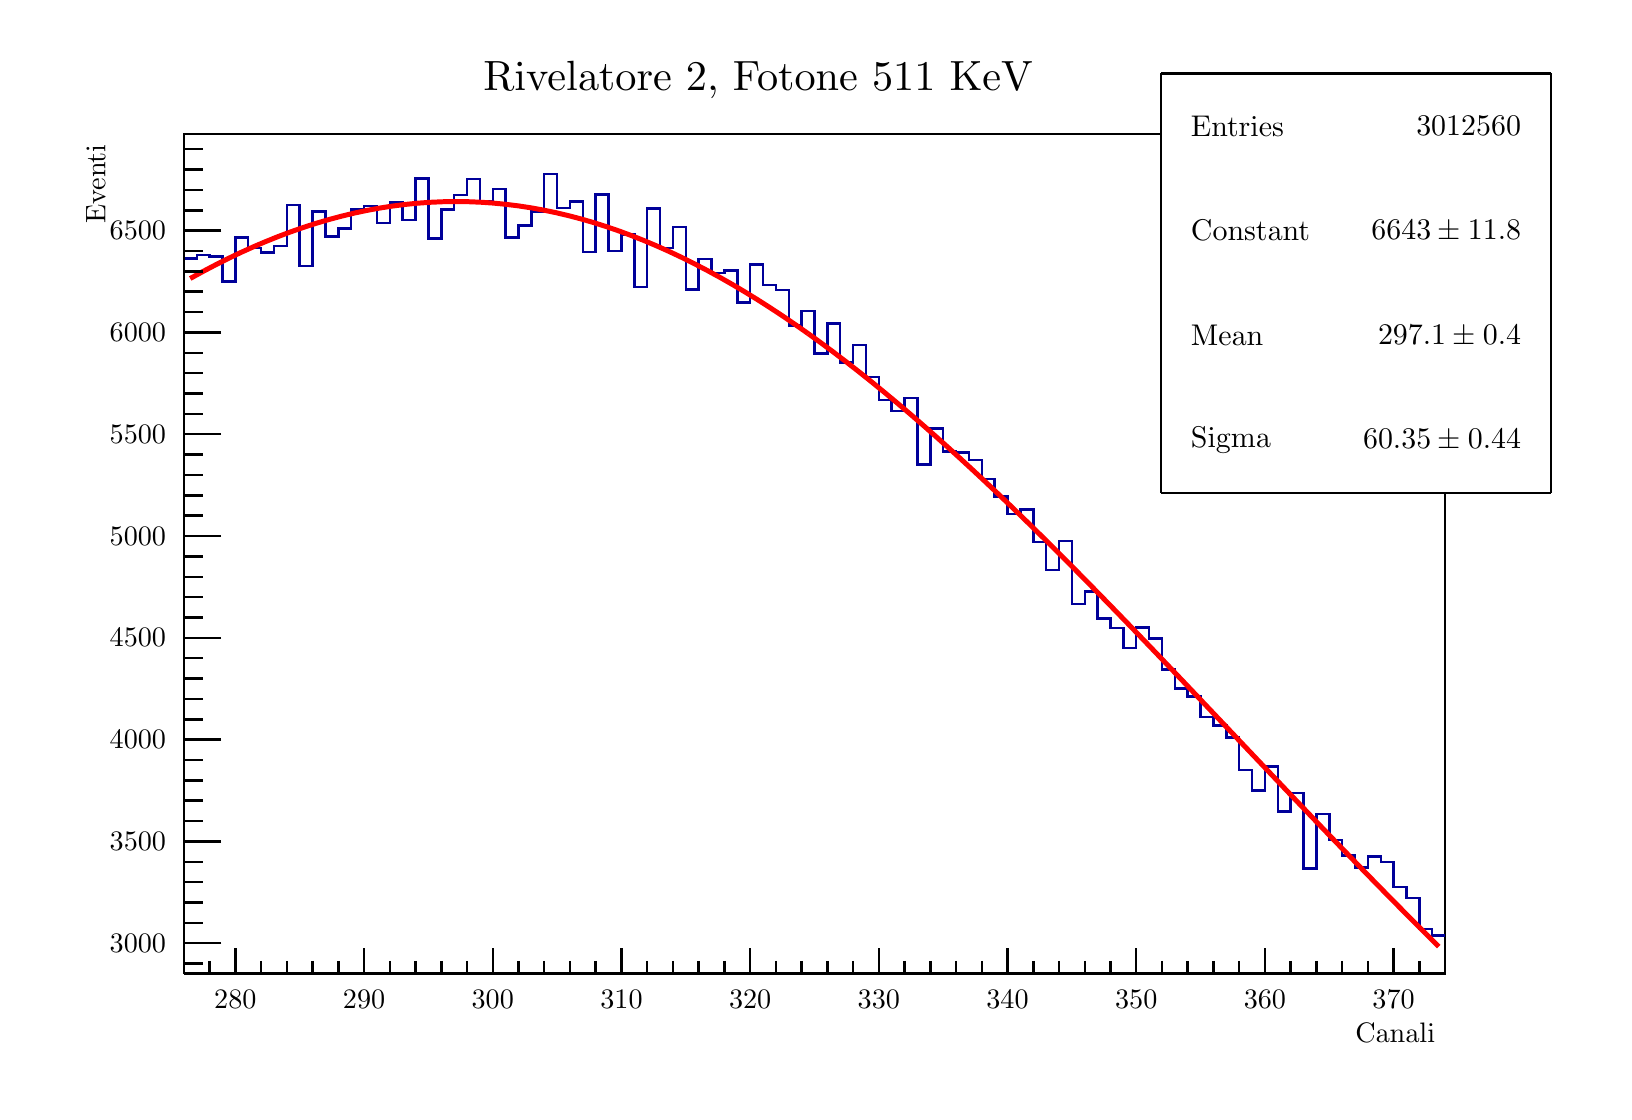
\begin{tikzpicture}
\pgfdeclareplotmark{cross} {
\pgfpathmoveto{\pgfpoint{-0.3\pgfplotmarksize}{\pgfplotmarksize}}
\pgfpathlineto{\pgfpoint{+0.3\pgfplotmarksize}{\pgfplotmarksize}}
\pgfpathlineto{\pgfpoint{+0.3\pgfplotmarksize}{0.3\pgfplotmarksize}}
\pgfpathlineto{\pgfpoint{+1\pgfplotmarksize}{0.3\pgfplotmarksize}}
\pgfpathlineto{\pgfpoint{+1\pgfplotmarksize}{-0.3\pgfplotmarksize}}
\pgfpathlineto{\pgfpoint{+0.3\pgfplotmarksize}{-0.3\pgfplotmarksize}}
\pgfpathlineto{\pgfpoint{+0.3\pgfplotmarksize}{-1.\pgfplotmarksize}}
\pgfpathlineto{\pgfpoint{-0.3\pgfplotmarksize}{-1.\pgfplotmarksize}}
\pgfpathlineto{\pgfpoint{-0.3\pgfplotmarksize}{-0.3\pgfplotmarksize}}
\pgfpathlineto{\pgfpoint{-1.\pgfplotmarksize}{-0.3\pgfplotmarksize}}
\pgfpathlineto{\pgfpoint{-1.\pgfplotmarksize}{0.3\pgfplotmarksize}}
\pgfpathlineto{\pgfpoint{-0.3\pgfplotmarksize}{0.3\pgfplotmarksize}}
\pgfpathclose
\pgfusepathqstroke
}
\pgfdeclareplotmark{cross*} {
\pgfpathmoveto{\pgfpoint{-0.3\pgfplotmarksize}{\pgfplotmarksize}}
\pgfpathlineto{\pgfpoint{+0.3\pgfplotmarksize}{\pgfplotmarksize}}
\pgfpathlineto{\pgfpoint{+0.3\pgfplotmarksize}{0.3\pgfplotmarksize}}
\pgfpathlineto{\pgfpoint{+1\pgfplotmarksize}{0.3\pgfplotmarksize}}
\pgfpathlineto{\pgfpoint{+1\pgfplotmarksize}{-0.3\pgfplotmarksize}}
\pgfpathlineto{\pgfpoint{+0.3\pgfplotmarksize}{-0.3\pgfplotmarksize}}
\pgfpathlineto{\pgfpoint{+0.3\pgfplotmarksize}{-1.\pgfplotmarksize}}
\pgfpathlineto{\pgfpoint{-0.3\pgfplotmarksize}{-1.\pgfplotmarksize}}
\pgfpathlineto{\pgfpoint{-0.3\pgfplotmarksize}{-0.3\pgfplotmarksize}}
\pgfpathlineto{\pgfpoint{-1.\pgfplotmarksize}{-0.3\pgfplotmarksize}}
\pgfpathlineto{\pgfpoint{-1.\pgfplotmarksize}{0.3\pgfplotmarksize}}
\pgfpathlineto{\pgfpoint{-0.3\pgfplotmarksize}{0.3\pgfplotmarksize}}
\pgfpathclose
\pgfusepathqfillstroke
}
\pgfdeclareplotmark{newstar} {
\pgfpathmoveto{\pgfqpoint{0pt}{\pgfplotmarksize}}
\pgfpathlineto{\pgfqpointpolar{44}{0.5\pgfplotmarksize}}
\pgfpathlineto{\pgfqpointpolar{18}{\pgfplotmarksize}}
\pgfpathlineto{\pgfqpointpolar{-20}{0.5\pgfplotmarksize}}
\pgfpathlineto{\pgfqpointpolar{-54}{\pgfplotmarksize}}
\pgfpathlineto{\pgfqpointpolar{-90}{0.5\pgfplotmarksize}}
\pgfpathlineto{\pgfqpointpolar{234}{\pgfplotmarksize}}
\pgfpathlineto{\pgfqpointpolar{198}{0.5\pgfplotmarksize}}
\pgfpathlineto{\pgfqpointpolar{162}{\pgfplotmarksize}}
\pgfpathlineto{\pgfqpointpolar{134}{0.5\pgfplotmarksize}}
\pgfpathclose
\pgfusepathqstroke
}
\pgfdeclareplotmark{newstar*} {
\pgfpathmoveto{\pgfqpoint{0pt}{\pgfplotmarksize}}
\pgfpathlineto{\pgfqpointpolar{44}{0.5\pgfplotmarksize}}
\pgfpathlineto{\pgfqpointpolar{18}{\pgfplotmarksize}}
\pgfpathlineto{\pgfqpointpolar{-20}{0.5\pgfplotmarksize}}
\pgfpathlineto{\pgfqpointpolar{-54}{\pgfplotmarksize}}
\pgfpathlineto{\pgfqpointpolar{-90}{0.5\pgfplotmarksize}}
\pgfpathlineto{\pgfqpointpolar{234}{\pgfplotmarksize}}
\pgfpathlineto{\pgfqpointpolar{198}{0.5\pgfplotmarksize}}
\pgfpathlineto{\pgfqpointpolar{162}{\pgfplotmarksize}}
\pgfpathlineto{\pgfqpointpolar{134}{0.5\pgfplotmarksize}}
\pgfpathclose
\pgfusepathqfillstroke
}
\definecolor{c}{rgb}{1,1,1};
\draw [color=c, fill=c] (0,0) rectangle (20,13.4957);
\draw [color=c, fill=c] (1.97708,1.48997) rectangle (17.9943,12.149);
\definecolor{c}{rgb}{0,0,0};
\draw [c,line width=0.9] (1.97708,1.48997) -- (1.97708,12.149) -- (17.9943,12.149) -- (17.9943,1.48997) -- (1.97708,1.48997);
\definecolor{c}{rgb}{1,1,1};
\draw [color=c, fill=c] (1.97708,1.48997) rectangle (17.9943,12.149);
\definecolor{c}{rgb}{0,0,0};
\draw [c,line width=0.9] (1.97708,1.48997) -- (1.97708,12.149) -- (17.9943,12.149) -- (17.9943,1.48997) -- (1.97708,1.48997);
\definecolor{c}{rgb}{0,0,0.6};
\draw [c,line width=0.9] (1.97708,10.5709) -- (2.14052,10.5709) -- (2.14052,10.6149) -- (2.30396,10.6149) -- (2.30396,10.5942) -- (2.4674,10.5942) -- (2.4674,10.2813) -- (2.63084,10.2813) -- (2.63084,10.8347) -- (2.79428,10.8347) -- (2.79428,10.7054)
 -- (2.95772,10.7054) -- (2.95772,10.6485) -- (3.12116,10.6485) -- (3.12116,10.7287) -- (3.2846,10.7287) -- (3.2846,11.2484) -- (3.44804,11.2484) -- (3.44804,10.4778) -- (3.61148,10.4778) -- (3.61148,11.1682) -- (3.77493,11.1682) -- (3.77493,10.8528)
 -- (3.93837,10.8528) -- (3.93837,10.9536) -- (4.10181,10.9536) -- (4.10181,11.1915) -- (4.26525,11.1915) -- (4.26525,11.2355) -- (4.42869,11.2355) -- (4.42869,11.0208) -- (4.59213,11.0208) -- (4.59213,11.2794) -- (4.75557,11.2794) --
 (4.75557,11.0596) -- (4.91901,11.0596) -- (4.91901,11.5845) -- (5.08245,11.5845) -- (5.08245,10.8269) -- (5.24589,10.8269) -- (5.24589,11.1915) -- (5.40933,11.1915) -- (5.40933,11.3777) -- (5.57277,11.3777) -- (5.57277,11.5794) -- (5.73621,11.5794)
 -- (5.73621,11.3001) -- (5.89965,11.3001) -- (5.89965,11.4527) -- (6.0631,11.4527) -- (6.0631,10.8347) -- (6.22654,10.8347) -- (6.22654,10.9924) -- (6.38998,10.9924) -- (6.38998,11.1656) -- (6.55342,11.1656) -- (6.55342,11.6414) -- (6.71686,11.6414)
 -- (6.71686,11.2148) -- (6.8803,11.2148) -- (6.8803,11.2949) -- (7.04374,11.2949) -- (7.04374,10.6537) -- (7.20718,10.6537) -- (7.20718,11.3854) -- (7.37062,11.3854) -- (7.37062,10.664) -- (7.53406,10.664) -- (7.53406,10.876) -- (7.6975,10.876) --
 (7.6975,10.2115) -- (7.86094,10.2115) -- (7.86094,11.2044) -- (8.02438,11.2044) -- (8.02438,10.7054) -- (8.18783,10.7054) -- (8.18783,10.9691) -- (8.35127,10.9691) -- (8.35127,10.1805) -- (8.51471,10.1805) -- (8.51471,10.5632) -- (8.67815,10.5632)
 -- (8.67815,10.3873) -- (8.84159,10.3873) -- (8.84159,10.4184) -- (9.00503,10.4184) -- (9.00503,10.015) -- (9.16847,10.015) -- (9.16847,10.4959) -- (9.33191,10.4959) -- (9.33191,10.2374) -- (9.49535,10.2374) -- (9.49535,10.1727) -- (9.65879,10.1727)
 -- (9.65879,9.72023) -- (9.82223,9.72023) -- (9.82223,9.90381) -- (9.98567,9.90381) -- (9.98567,9.36598) -- (10.1491,9.36598) -- (10.1491,9.7435) -- (10.3126,9.7435) -- (10.3126,9.25221) -- (10.476,9.25221) -- (10.476,9.46941) -- (10.6394,9.46941)
 -- (10.6394,9.06862) -- (10.8029,9.06862) -- (10.8029,8.77385) -- (10.9663,8.77385) -- (10.9663,8.63422) -- (11.1298,8.63422) -- (11.1298,8.79712) -- (11.2932,8.79712) -- (11.2932,7.95417) -- (11.4566,7.95417) -- (11.4566,8.40926) --
 (11.6201,8.40926) -- (11.6201,8.11707) -- (11.7835,8.11707) -- (11.7835,8.10673) -- (11.947,8.10673) -- (11.947,8.01106) -- (12.1104,8.01106) -- (12.1104,7.768) -- (12.2738,7.768) -- (12.2738,7.54821) -- (12.4373,7.54821) -- (12.4373,7.32584) --
 (12.6007,7.32584) -- (12.6007,7.38272) -- (12.7642,7.38272) -- (12.7642,6.96901) -- (12.9276,6.96901) -- (12.9276,6.61735) -- (13.091,6.61735) -- (13.091,6.98452) -- (13.2545,6.98452) -- (13.2545,6.18036) -- (13.4179,6.18036) -- (13.4179,6.34067) --
 (13.5814,6.34067) -- (13.5814,5.99677) -- (13.7448,5.99677) -- (13.7448,5.87783) -- (13.9083,5.87783) -- (13.9083,5.62701) -- (14.0717,5.62701) -- (14.0717,5.88559) -- (14.2351,5.88559) -- (14.2351,5.74596) -- (14.3986,5.74596) -- (14.3986,5.35034)
 -- (14.562,5.35034) -- (14.562,5.10987) -- (14.7255,5.10987) -- (14.7255,5.01161) -- (14.8889,5.01161) -- (14.8889,4.75045) -- (15.0523,4.75045) -- (15.0523,4.64185) -- (15.2158,4.64185) -- (15.2158,4.48671) -- (15.3792,4.48671) -- (15.3792,4.07299)
 -- (15.5427,4.07299) -- (15.5427,3.81441) -- (15.7061,3.81441) -- (15.7061,4.11953) -- (15.8695,4.11953) -- (15.8695,3.55067) -- (16.033,3.55067) -- (16.033,3.7808) -- (16.1964,3.7808) -- (16.1964,2.82149) -- (16.3599,2.82149) -- (16.3599,3.51447)
 -- (16.5233,3.51447) -- (16.5233,3.1835) -- (16.6867,3.1835) -- (16.6867,2.98957) -- (16.8502,2.98957) -- (16.8502,2.83701) -- (17.0136,2.83701) -- (17.0136,2.97405) -- (17.1771,2.97405) -- (17.1771,2.90682) -- (17.3405,2.90682) -- (17.3405,2.59136)
 -- (17.5039,2.59136) -- (17.5039,2.44656) -- (17.6674,2.44656) -- (17.6674,2.05353) -- (17.8308,2.05353) -- (17.8308,1.97337) -- (17.9943,1.97337);
\definecolor{c}{rgb}{1,1,1};
\draw [color=c, fill=c] (14.384,7.59312) rectangle (19.341,12.9226);
\definecolor{c}{rgb}{0,0,0};
\draw [c,line width=0.9] (14.384,7.59312) -- (19.341,7.59312);
\draw [c,line width=0.9] (19.341,7.59312) -- (19.341,12.9226);
\draw [c,line width=0.9] (19.341,12.9226) -- (14.384,12.9226);
\draw [c,line width=0.9] (14.384,12.9226) -- (14.384,7.59312);
\draw [anchor= west] (14.6318,12.2564) node[scale=1.08185, color=c, rotate=0]{Entries };
\draw [anchor= east] (19.0931,12.2564) node[scale=1.08185, color=c, rotate=0]{ 3012560};
\draw [anchor= west] (14.6318,10.9241) node[scale=1.08185, color=c, rotate=0]{Constant };
\draw [anchor= east] (19.0931,10.9241) node[scale=1.08185, color=c, rotate=0]{$  6643 \pm 11.8$};
\draw [anchor= west] (14.6318,9.59169) node[scale=1.08185, color=c, rotate=0]{Mean     };
\draw [anchor= east] (19.0931,9.59169) node[scale=1.08185, color=c, rotate=0]{$ 297.1 \pm 0.4$};
\draw [anchor= west] (14.6318,8.25931) node[scale=1.08185, color=c, rotate=0]{Sigma    };
\draw [anchor= east] (19.0931,8.25931) node[scale=1.08185, color=c, rotate=0]{$ 60.35 \pm 0.44$};
\definecolor{c}{rgb}{1,0,0};
\draw [c,line width=1.8] (2.05716,10.3171) -- (2.21734,10.4053) -- (2.37751,10.4896) -- (2.53768,10.57) -- (2.69785,10.6464) -- (2.85802,10.7188) -- (3.01819,10.7872) -- (3.17837,10.8514) -- (3.33854,10.9114) -- (3.49871,10.9672) -- (3.65888,11.0187)
 -- (3.81905,11.0659) -- (3.97923,11.1088) -- (4.1394,11.1473) -- (4.29957,11.1814) -- (4.45974,11.211) -- (4.61991,11.2362) -- (4.78009,11.2568) -- (4.94026,11.273) -- (5.10043,11.2847) -- (5.2606,11.2918) -- (5.42077,11.2945) -- (5.58095,11.2926)
 -- (5.74112,11.2861) -- (5.90129,11.2752) -- (6.06146,11.2597) -- (6.22163,11.2398) -- (6.38181,11.2153) -- (6.54198,11.1864) -- (6.70215,11.153) -- (6.86232,11.1152) -- (7.02249,11.0731) -- (7.18266,11.0266) -- (7.34284,10.9757) --
 (7.50301,10.9206) -- (7.66318,10.8613) -- (7.82335,10.7977) -- (7.98352,10.73) -- (8.1437,10.6583) -- (8.30387,10.5825) -- (8.46404,10.5027) -- (8.62421,10.419) -- (8.78438,10.3315) -- (8.94456,10.2402) -- (9.10473,10.1451) -- (9.2649,10.0465) --
 (9.42507,9.94423) -- (9.58524,9.83851) -- (9.74542,9.72938) -- (9.90559,9.61692);
\draw [c,line width=1.8] (9.90559,9.61692) -- (10.0658,9.50121) -- (10.2259,9.38234) -- (10.3861,9.26039) -- (10.5463,9.13546) -- (10.7064,9.00763) -- (10.8666,8.877) -- (11.0268,8.74366) -- (11.187,8.6077) -- (11.3471,8.46922) -- (11.5073,8.32832)
 -- (11.6675,8.18509) -- (11.8277,8.03963) -- (11.9878,7.89205) -- (12.148,7.74243) -- (12.3082,7.59089) -- (12.4683,7.43752) -- (12.6285,7.28243) -- (12.7887,7.12571) -- (12.9489,6.96747) -- (13.109,6.80781) -- (13.2692,6.64683) -- (13.4294,6.48462)
 -- (13.5895,6.3213) -- (13.7497,6.15697) -- (13.9099,5.99171) -- (14.0701,5.82564) -- (14.2302,5.65884) -- (14.3904,5.49142) -- (14.5506,5.32348) -- (14.7107,5.1551) -- (14.8709,4.98639) -- (15.0311,4.81744) -- (15.1913,4.64833) -- (15.3514,4.47917)
 -- (15.5116,4.31003) -- (15.6718,4.14102) -- (15.8319,3.9722) -- (15.9921,3.80368) -- (16.1523,3.63553) -- (16.3125,3.46783) -- (16.4726,3.30067) -- (16.6328,3.13411) -- (16.793,2.96825) -- (16.9532,2.80314) -- (17.1133,2.63887) -- (17.2735,2.4755)
 -- (17.4337,2.3131) -- (17.5938,2.15174) -- (17.754,1.99148);
\draw [c,line width=1.8] (17.754,1.99148) -- (17.9142,1.83238);
\definecolor{c}{rgb}{0,0,0};
\draw [c,line width=0.9] (1.97708,1.48997) -- (17.9943,1.48997);
\draw [anchor= east] (17.9943,0.734212) node[scale=1.01821, color=c, rotate=0]{Canali};
\draw [c,line width=0.9] (2.63084,1.81422) -- (2.63084,1.48997);
\draw [c,line width=0.9] (2.95772,1.65209) -- (2.95772,1.48997);
\draw [c,line width=0.9] (3.2846,1.65209) -- (3.2846,1.48997);
\draw [c,line width=0.9] (3.61148,1.65209) -- (3.61148,1.48997);
\draw [c,line width=0.9] (3.93837,1.65209) -- (3.93837,1.48997);
\draw [c,line width=0.9] (4.26525,1.81422) -- (4.26525,1.48997);
\draw [c,line width=0.9] (4.59213,1.65209) -- (4.59213,1.48997);
\draw [c,line width=0.9] (4.91901,1.65209) -- (4.91901,1.48997);
\draw [c,line width=0.9] (5.24589,1.65209) -- (5.24589,1.48997);
\draw [c,line width=0.9] (5.57277,1.65209) -- (5.57277,1.48997);
\draw [c,line width=0.9] (5.89965,1.81422) -- (5.89965,1.48997);
\draw [c,line width=0.9] (6.22654,1.65209) -- (6.22654,1.48997);
\draw [c,line width=0.9] (6.55342,1.65209) -- (6.55342,1.48997);
\draw [c,line width=0.9] (6.8803,1.65209) -- (6.8803,1.48997);
\draw [c,line width=0.9] (7.20718,1.65209) -- (7.20718,1.48997);
\draw [c,line width=0.9] (7.53406,1.81422) -- (7.53406,1.48997);
\draw [c,line width=0.9] (7.86094,1.65209) -- (7.86094,1.48997);
\draw [c,line width=0.9] (8.18783,1.65209) -- (8.18783,1.48997);
\draw [c,line width=0.9] (8.51471,1.65209) -- (8.51471,1.48997);
\draw [c,line width=0.9] (8.84159,1.65209) -- (8.84159,1.48997);
\draw [c,line width=0.9] (9.16847,1.81422) -- (9.16847,1.48997);
\draw [c,line width=0.9] (9.49535,1.65209) -- (9.49535,1.48997);
\draw [c,line width=0.9] (9.82223,1.65209) -- (9.82223,1.48997);
\draw [c,line width=0.9] (10.1491,1.65209) -- (10.1491,1.48997);
\draw [c,line width=0.9] (10.476,1.65209) -- (10.476,1.48997);
\draw [c,line width=0.9] (10.8029,1.81422) -- (10.8029,1.48997);
\draw [c,line width=0.9] (11.1298,1.65209) -- (11.1298,1.48997);
\draw [c,line width=0.9] (11.4566,1.65209) -- (11.4566,1.48997);
\draw [c,line width=0.9] (11.7835,1.65209) -- (11.7835,1.48997);
\draw [c,line width=0.9] (12.1104,1.65209) -- (12.1104,1.48997);
\draw [c,line width=0.9] (12.4373,1.81422) -- (12.4373,1.48997);
\draw [c,line width=0.9] (12.7642,1.65209) -- (12.7642,1.48997);
\draw [c,line width=0.9] (13.091,1.65209) -- (13.091,1.48997);
\draw [c,line width=0.9] (13.4179,1.65209) -- (13.4179,1.48997);
\draw [c,line width=0.9] (13.7448,1.65209) -- (13.7448,1.48997);
\draw [c,line width=0.9] (14.0717,1.81422) -- (14.0717,1.48997);
\draw [c,line width=0.9] (14.3986,1.65209) -- (14.3986,1.48997);
\draw [c,line width=0.9] (14.7255,1.65209) -- (14.7255,1.48997);
\draw [c,line width=0.9] (15.0523,1.65209) -- (15.0523,1.48997);
\draw [c,line width=0.9] (15.3792,1.65209) -- (15.3792,1.48997);
\draw [c,line width=0.9] (15.7061,1.81422) -- (15.7061,1.48997);
\draw [c,line width=0.9] (16.033,1.65209) -- (16.033,1.48997);
\draw [c,line width=0.9] (16.3599,1.65209) -- (16.3599,1.48997);
\draw [c,line width=0.9] (16.6867,1.65209) -- (16.6867,1.48997);
\draw [c,line width=0.9] (17.0136,1.65209) -- (17.0136,1.48997);
\draw [c,line width=0.9] (17.3405,1.81422) -- (17.3405,1.48997);
\draw [c,line width=0.9] (2.63084,1.81422) -- (2.63084,1.48997);
\draw [c,line width=0.9] (2.30396,1.65209) -- (2.30396,1.48997);
\draw [c,line width=0.9] (1.97708,1.65209) -- (1.97708,1.48997);
\draw [c,line width=0.9] (17.3405,1.81422) -- (17.3405,1.48997);
\draw [c,line width=0.9] (17.6674,1.65209) -- (17.6674,1.48997);
\draw [c,line width=0.9] (17.9943,1.65209) -- (17.9943,1.48997);
\draw [anchor=base] (2.63084,1.04461) node[scale=1.01821, color=c, rotate=0]{280};
\draw [anchor=base] (4.26525,1.04461) node[scale=1.01821, color=c, rotate=0]{290};
\draw [anchor=base] (5.89965,1.04461) node[scale=1.01821, color=c, rotate=0]{300};
\draw [anchor=base] (7.53406,1.04461) node[scale=1.01821, color=c, rotate=0]{310};
\draw [anchor=base] (9.16847,1.04461) node[scale=1.01821, color=c, rotate=0]{320};
\draw [anchor=base] (10.8029,1.04461) node[scale=1.01821, color=c, rotate=0]{330};
\draw [anchor=base] (12.4373,1.04461) node[scale=1.01821, color=c, rotate=0]{340};
\draw [anchor=base] (14.0717,1.04461) node[scale=1.01821, color=c, rotate=0]{350};
\draw [anchor=base] (15.7061,1.04461) node[scale=1.01821, color=c, rotate=0]{360};
\draw [anchor=base] (17.3405,1.04461) node[scale=1.01821, color=c, rotate=0]{370};
\draw [c,line width=0.9] (1.97708,1.48997) -- (1.97708,12.149);
\draw [anchor= east] (0.857077,12.149) node[scale=1.01821, color=c, rotate=90]{Eventi};
\draw [c,line width=0.9] (2.45096,1.87512) -- (1.97708,1.87512);
\draw [c,line width=0.9] (2.21402,2.13369) -- (1.97708,2.13369);
\draw [c,line width=0.9] (2.21402,2.39226) -- (1.97708,2.39226);
\draw [c,line width=0.9] (2.21402,2.65084) -- (1.97708,2.65084);
\draw [c,line width=0.9] (2.21402,2.90941) -- (1.97708,2.90941);
\draw [c,line width=0.9] (2.45096,3.16798) -- (1.97708,3.16798);
\draw [c,line width=0.9] (2.21402,3.42656) -- (1.97708,3.42656);
\draw [c,line width=0.9] (2.21402,3.68513) -- (1.97708,3.68513);
\draw [c,line width=0.9] (2.21402,3.9437) -- (1.97708,3.9437);
\draw [c,line width=0.9] (2.21402,4.20227) -- (1.97708,4.20227);
\draw [c,line width=0.9] (2.45096,4.46085) -- (1.97708,4.46085);
\draw [c,line width=0.9] (2.21402,4.71942) -- (1.97708,4.71942);
\draw [c,line width=0.9] (2.21402,4.97799) -- (1.97708,4.97799);
\draw [c,line width=0.9] (2.21402,5.23657) -- (1.97708,5.23657);
\draw [c,line width=0.9] (2.21402,5.49514) -- (1.97708,5.49514);
\draw [c,line width=0.9] (2.45096,5.75371) -- (1.97708,5.75371);
\draw [c,line width=0.9] (2.21402,6.01229) -- (1.97708,6.01229);
\draw [c,line width=0.9] (2.21402,6.27086) -- (1.97708,6.27086);
\draw [c,line width=0.9] (2.21402,6.52943) -- (1.97708,6.52943);
\draw [c,line width=0.9] (2.21402,6.78801) -- (1.97708,6.78801);
\draw [c,line width=0.9] (2.45096,7.04658) -- (1.97708,7.04658);
\draw [c,line width=0.9] (2.21402,7.30515) -- (1.97708,7.30515);
\draw [c,line width=0.9] (2.21402,7.56373) -- (1.97708,7.56373);
\draw [c,line width=0.9] (2.21402,7.8223) -- (1.97708,7.8223);
\draw [c,line width=0.9] (2.21402,8.08087) -- (1.97708,8.08087);
\draw [c,line width=0.9] (2.45096,8.33945) -- (1.97708,8.33945);
\draw [c,line width=0.9] (2.21402,8.59802) -- (1.97708,8.59802);
\draw [c,line width=0.9] (2.21402,8.85659) -- (1.97708,8.85659);
\draw [c,line width=0.9] (2.21402,9.11516) -- (1.97708,9.11516);
\draw [c,line width=0.9] (2.21402,9.37374) -- (1.97708,9.37374);
\draw [c,line width=0.9] (2.45096,9.63231) -- (1.97708,9.63231);
\draw [c,line width=0.9] (2.21402,9.89088) -- (1.97708,9.89088);
\draw [c,line width=0.9] (2.21402,10.1495) -- (1.97708,10.1495);
\draw [c,line width=0.9] (2.21402,10.408) -- (1.97708,10.408);
\draw [c,line width=0.9] (2.21402,10.6666) -- (1.97708,10.6666);
\draw [c,line width=0.9] (2.45096,10.9252) -- (1.97708,10.9252);
\draw [c,line width=0.9] (2.45096,1.87512) -- (1.97708,1.87512);
\draw [c,line width=0.9] (2.21402,1.61654) -- (1.97708,1.61654);
\draw [c,line width=0.9] (2.45096,10.9252) -- (1.97708,10.9252);
\draw [c,line width=0.9] (2.21402,11.1838) -- (1.97708,11.1838);
\draw [c,line width=0.9] (2.21402,11.4423) -- (1.97708,11.4423);
\draw [c,line width=0.9] (2.21402,11.7009) -- (1.97708,11.7009);
\draw [c,line width=0.9] (2.21402,11.9595) -- (1.97708,11.9595);
\draw [anchor= east] (1.87708,1.87512) node[scale=1.01821, color=c, rotate=0]{3000};
\draw [anchor= east] (1.87708,3.16798) node[scale=1.01821, color=c, rotate=0]{3500};
\draw [anchor= east] (1.87708,4.46085) node[scale=1.01821, color=c, rotate=0]{4000};
\draw [anchor= east] (1.87708,5.75371) node[scale=1.01821, color=c, rotate=0]{4500};
\draw [anchor= east] (1.87708,7.04658) node[scale=1.01821, color=c, rotate=0]{5000};
\draw [anchor= east] (1.87708,8.33945) node[scale=1.01821, color=c, rotate=0]{5500};
\draw [anchor= east] (1.87708,9.63231) node[scale=1.01821, color=c, rotate=0]{6000};
\draw [anchor= east] (1.87708,10.9252) node[scale=1.01821, color=c, rotate=0]{6500};
\definecolor{c}{rgb}{1,1,1};
\draw [color=c, fill=c] (14.384,7.59312) rectangle (19.341,12.9226);
\definecolor{c}{rgb}{0,0,0};
\draw [c,line width=0.9] (14.384,7.59312) -- (19.341,7.59312);
\draw [c,line width=0.9] (19.341,7.59312) -- (19.341,12.9226);
\draw [c,line width=0.9] (19.341,12.9226) -- (14.384,12.9226);
\draw [c,line width=0.9] (14.384,12.9226) -- (14.384,7.59312);
\draw [anchor= west] (14.6318,12.2564) node[scale=1.08185, color=c, rotate=0]{Entries };
\draw [anchor= east] (19.0931,12.2564) node[scale=1.08185, color=c, rotate=0]{ 3012560};
\draw [anchor= west] (14.6318,10.9241) node[scale=1.08185, color=c, rotate=0]{Constant };
\draw [anchor= east] (19.0931,10.9241) node[scale=1.08185, color=c, rotate=0]{$  6643 \pm 11.8$};
\draw [anchor= west] (14.6318,9.59169) node[scale=1.08185, color=c, rotate=0]{Mean     };
\draw [anchor= east] (19.0931,9.59169) node[scale=1.08185, color=c, rotate=0]{$ 297.1 \pm 0.4$};
\draw [anchor= west] (14.6318,8.25931) node[scale=1.08185, color=c, rotate=0]{Sigma    };
\draw [anchor= east] (19.0931,8.25931) node[scale=1.08185, color=c, rotate=0]{$ 60.35 \pm 0.44$};
\draw (9.26934,12.8367) node[scale=1.52731, color=c, rotate=0]{Rivelatore 2, Fotone 511 KeV};
\end{tikzpicture}

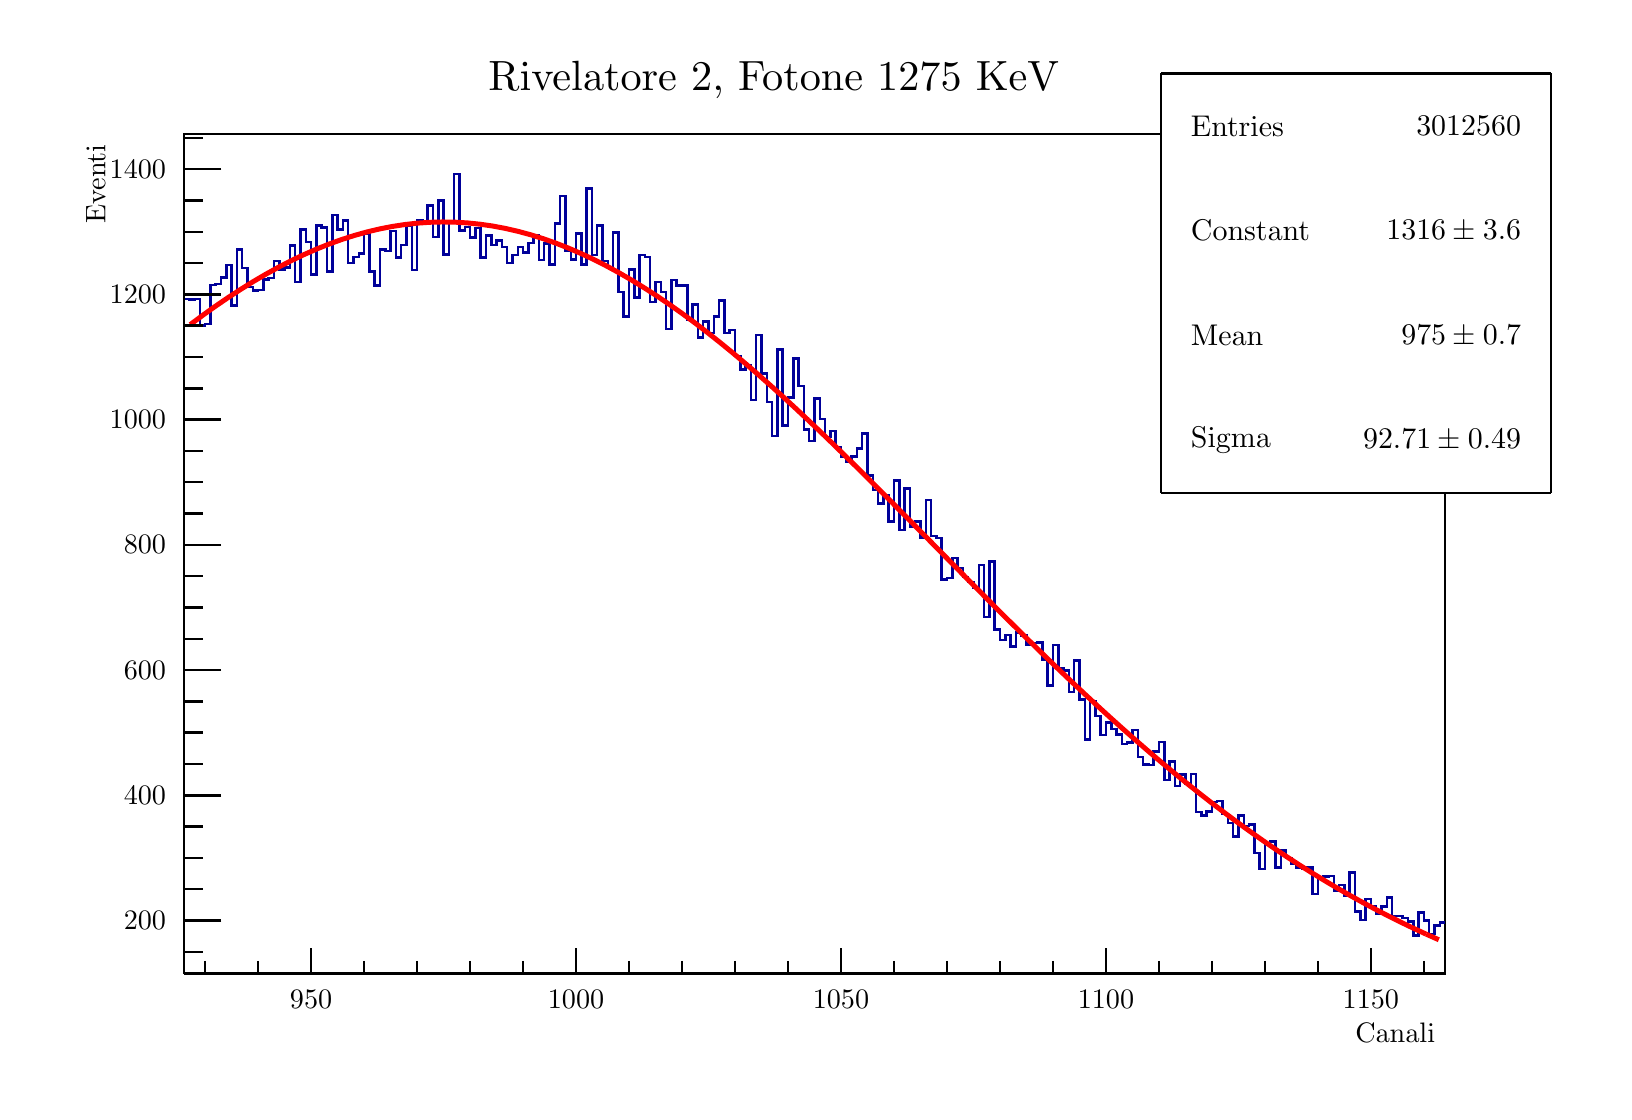
\begin{tikzpicture}
\pgfdeclareplotmark{cross} {
\pgfpathmoveto{\pgfpoint{-0.3\pgfplotmarksize}{\pgfplotmarksize}}
\pgfpathlineto{\pgfpoint{+0.3\pgfplotmarksize}{\pgfplotmarksize}}
\pgfpathlineto{\pgfpoint{+0.3\pgfplotmarksize}{0.3\pgfplotmarksize}}
\pgfpathlineto{\pgfpoint{+1\pgfplotmarksize}{0.3\pgfplotmarksize}}
\pgfpathlineto{\pgfpoint{+1\pgfplotmarksize}{-0.3\pgfplotmarksize}}
\pgfpathlineto{\pgfpoint{+0.3\pgfplotmarksize}{-0.3\pgfplotmarksize}}
\pgfpathlineto{\pgfpoint{+0.3\pgfplotmarksize}{-1.\pgfplotmarksize}}
\pgfpathlineto{\pgfpoint{-0.3\pgfplotmarksize}{-1.\pgfplotmarksize}}
\pgfpathlineto{\pgfpoint{-0.3\pgfplotmarksize}{-0.3\pgfplotmarksize}}
\pgfpathlineto{\pgfpoint{-1.\pgfplotmarksize}{-0.3\pgfplotmarksize}}
\pgfpathlineto{\pgfpoint{-1.\pgfplotmarksize}{0.3\pgfplotmarksize}}
\pgfpathlineto{\pgfpoint{-0.3\pgfplotmarksize}{0.3\pgfplotmarksize}}
\pgfpathclose
\pgfusepathqstroke
}
\pgfdeclareplotmark{cross*} {
\pgfpathmoveto{\pgfpoint{-0.3\pgfplotmarksize}{\pgfplotmarksize}}
\pgfpathlineto{\pgfpoint{+0.3\pgfplotmarksize}{\pgfplotmarksize}}
\pgfpathlineto{\pgfpoint{+0.3\pgfplotmarksize}{0.3\pgfplotmarksize}}
\pgfpathlineto{\pgfpoint{+1\pgfplotmarksize}{0.3\pgfplotmarksize}}
\pgfpathlineto{\pgfpoint{+1\pgfplotmarksize}{-0.3\pgfplotmarksize}}
\pgfpathlineto{\pgfpoint{+0.3\pgfplotmarksize}{-0.3\pgfplotmarksize}}
\pgfpathlineto{\pgfpoint{+0.3\pgfplotmarksize}{-1.\pgfplotmarksize}}
\pgfpathlineto{\pgfpoint{-0.3\pgfplotmarksize}{-1.\pgfplotmarksize}}
\pgfpathlineto{\pgfpoint{-0.3\pgfplotmarksize}{-0.3\pgfplotmarksize}}
\pgfpathlineto{\pgfpoint{-1.\pgfplotmarksize}{-0.3\pgfplotmarksize}}
\pgfpathlineto{\pgfpoint{-1.\pgfplotmarksize}{0.3\pgfplotmarksize}}
\pgfpathlineto{\pgfpoint{-0.3\pgfplotmarksize}{0.3\pgfplotmarksize}}
\pgfpathclose
\pgfusepathqfillstroke
}
\pgfdeclareplotmark{newstar} {
\pgfpathmoveto{\pgfqpoint{0pt}{\pgfplotmarksize}}
\pgfpathlineto{\pgfqpointpolar{44}{0.5\pgfplotmarksize}}
\pgfpathlineto{\pgfqpointpolar{18}{\pgfplotmarksize}}
\pgfpathlineto{\pgfqpointpolar{-20}{0.5\pgfplotmarksize}}
\pgfpathlineto{\pgfqpointpolar{-54}{\pgfplotmarksize}}
\pgfpathlineto{\pgfqpointpolar{-90}{0.5\pgfplotmarksize}}
\pgfpathlineto{\pgfqpointpolar{234}{\pgfplotmarksize}}
\pgfpathlineto{\pgfqpointpolar{198}{0.5\pgfplotmarksize}}
\pgfpathlineto{\pgfqpointpolar{162}{\pgfplotmarksize}}
\pgfpathlineto{\pgfqpointpolar{134}{0.5\pgfplotmarksize}}
\pgfpathclose
\pgfusepathqstroke
}
\pgfdeclareplotmark{newstar*} {
\pgfpathmoveto{\pgfqpoint{0pt}{\pgfplotmarksize}}
\pgfpathlineto{\pgfqpointpolar{44}{0.5\pgfplotmarksize}}
\pgfpathlineto{\pgfqpointpolar{18}{\pgfplotmarksize}}
\pgfpathlineto{\pgfqpointpolar{-20}{0.5\pgfplotmarksize}}
\pgfpathlineto{\pgfqpointpolar{-54}{\pgfplotmarksize}}
\pgfpathlineto{\pgfqpointpolar{-90}{0.5\pgfplotmarksize}}
\pgfpathlineto{\pgfqpointpolar{234}{\pgfplotmarksize}}
\pgfpathlineto{\pgfqpointpolar{198}{0.5\pgfplotmarksize}}
\pgfpathlineto{\pgfqpointpolar{162}{\pgfplotmarksize}}
\pgfpathlineto{\pgfqpointpolar{134}{0.5\pgfplotmarksize}}
\pgfpathclose
\pgfusepathqfillstroke
}
\definecolor{c}{rgb}{1,1,1};
\draw [color=c, fill=c] (0,0) rectangle (20,13.4957);
\draw [color=c, fill=c] (1.97708,1.48997) rectangle (17.9943,12.149);
\definecolor{c}{rgb}{0,0,0};
\draw [c,line width=0.9] (1.97708,1.48997) -- (1.97708,12.149) -- (17.9943,12.149) -- (17.9943,1.48997) -- (1.97708,1.48997);
\definecolor{c}{rgb}{1,1,1};
\draw [color=c, fill=c] (1.97708,1.48997) rectangle (17.9943,12.149);
\definecolor{c}{rgb}{0,0,0};
\draw [c,line width=0.9] (1.97708,1.48997) -- (1.97708,12.149) -- (17.9943,12.149) -- (17.9943,1.48997) -- (1.97708,1.48997);
\definecolor{c}{rgb}{0,0,0.6};
\draw [c,line width=0.9] (1.97708,10.0592) -- (2.04438,10.0592) -- (2.04438,10.0513) -- (2.11168,10.0513) -- (2.11168,10.0592) -- (2.17897,10.0592) -- (2.17897,9.71735) -- (2.24627,9.71735) -- (2.24627,9.74121) -- (2.31357,9.74121) --
 (2.31357,10.2342) -- (2.38087,10.2342) -- (2.38087,10.2501) -- (2.44817,10.2501) -- (2.44817,10.3296) -- (2.51547,10.3296) -- (2.51547,10.4886) -- (2.58277,10.4886) -- (2.58277,9.97178) -- (2.65007,9.97178) -- (2.65007,10.6873) -- (2.71737,10.6873)
 -- (2.71737,10.4488) -- (2.78467,10.4488) -- (2.78467,10.2103) -- (2.85197,10.2103) -- (2.85197,10.1626) -- (2.91927,10.1626) -- (2.91927,10.1705) -- (2.98656,10.1705) -- (2.98656,10.3057) -- (3.05386,10.3057) -- (3.05386,10.3216) --
 (3.12116,10.3216) -- (3.12116,10.5363) -- (3.18846,10.5363) -- (3.18846,10.4329) -- (3.25576,10.4329) -- (3.25576,10.4568) -- (3.32306,10.4568) -- (3.32306,10.735) -- (3.39036,10.735) -- (3.39036,10.2739) -- (3.45766,10.2739) -- (3.45766,10.9418) --
 (3.52496,10.9418) -- (3.52496,10.7827) -- (3.59226,10.7827) -- (3.59226,10.3693) -- (3.65956,10.3693) -- (3.65956,10.9895) -- (3.72685,10.9895) -- (3.72685,10.9656) -- (3.79415,10.9656) -- (3.79415,10.4091) -- (3.86145,10.4091) -- (3.86145,11.1246)
 -- (3.92875,11.1246) -- (3.92875,10.9418) -- (3.99605,10.9418) -- (3.99605,11.0531) -- (4.06335,11.0531) -- (4.06335,10.5124) -- (4.13065,10.5124) -- (4.13065,10.5919) -- (4.19795,10.5919) -- (4.19795,10.6317) -- (4.26525,10.6317) --
 (4.26525,10.8861) -- (4.33255,10.8861) -- (4.33255,10.4091) -- (4.39985,10.4091) -- (4.39985,10.2262) -- (4.46714,10.2262) -- (4.46714,10.6873) -- (4.53444,10.6873) -- (4.53444,10.6635) -- (4.60174,10.6635) -- (4.60174,10.9179) -- (4.66904,10.9179)
 -- (4.66904,10.584) -- (4.73634,10.584) -- (4.73634,10.743) -- (4.80364,10.743) -- (4.80364,10.9895) -- (4.87094,10.9895) -- (4.87094,10.425) -- (4.93824,10.425) -- (4.93824,11.0531) -- (5.00554,11.0531) -- (5.00554,11.0133) -- (5.07284,11.0133) --
 (5.07284,11.2439) -- (5.14014,11.2439) -- (5.14014,10.8464) -- (5.20744,10.8464) -- (5.20744,11.3075) -- (5.27473,11.3075) -- (5.27473,10.6237) -- (5.34203,10.6237) -- (5.34203,11.0451) -- (5.40933,11.0451) -- (5.40933,11.6414) -- (5.47663,11.6414)
 -- (5.47663,10.9259) -- (5.54393,10.9259) -- (5.54393,10.9736) -- (5.61123,10.9736) -- (5.61123,10.8384) -- (5.67853,10.8384) -- (5.67853,10.9577) -- (5.74583,10.9577) -- (5.74583,10.584) -- (5.81313,10.584) -- (5.81313,10.8623) -- (5.88043,10.8623)
 -- (5.88043,10.743) -- (5.94773,10.743) -- (5.94773,10.7986) -- (6.01503,10.7986) -- (6.01503,10.7191) -- (6.08232,10.7191) -- (6.08232,10.5124) -- (6.14962,10.5124) -- (6.14962,10.6158) -- (6.21692,10.6158) -- (6.21692,10.7191) -- (6.28422,10.7191)
 -- (6.28422,10.6476) -- (6.35152,10.6476) -- (6.35152,10.7668) -- (6.41882,10.7668) -- (6.41882,10.8623) -- (6.48612,10.8623) -- (6.48612,10.5522) -- (6.55342,10.5522) -- (6.55342,10.7589) -- (6.62072,10.7589) -- (6.62072,10.4965) --
 (6.68802,10.4965) -- (6.68802,11.0133) -- (6.75532,11.0133) -- (6.75532,11.3631) -- (6.82261,11.3631) -- (6.82261,10.6635) -- (6.88991,10.6635) -- (6.88991,10.5601) -- (6.95721,10.5601) -- (6.95721,10.8861) -- (7.02451,10.8861) -- (7.02451,10.4965)
 -- (7.09181,10.4965) -- (7.09181,11.4586) -- (7.15911,11.4586) -- (7.15911,10.6158) -- (7.22641,10.6158) -- (7.22641,10.9895) -- (7.29371,10.9895) -- (7.29371,10.5363) -- (7.36101,10.5363) -- (7.36101,10.4488) -- (7.42831,10.4488) --
 (7.42831,10.902) -- (7.49561,10.902) -- (7.49561,10.1467) -- (7.5629,10.1467) -- (7.5629,9.83662) -- (7.6302,9.83662) -- (7.6302,10.4329) -- (7.6975,10.4329) -- (7.6975,10.0751) -- (7.7648,10.0751) -- (7.7648,10.6158) -- (7.8321,10.6158) --
 (7.8321,10.5919) -- (7.8994,10.5919) -- (7.8994,10.0195) -- (7.9667,10.0195) -- (7.9667,10.2739) -- (8.034,10.2739) -- (8.034,10.1467) -- (8.1013,10.1467) -- (8.1013,9.6776) -- (8.1686,9.6776) -- (8.1686,10.2978) -- (8.2359,10.2978) --
 (8.2359,10.2262) -- (8.30319,10.2262) -- (8.30319,10.2262) -- (8.37049,10.2262) -- (8.37049,9.78891) -- (8.43779,9.78891) -- (8.43779,9.98768) -- (8.50509,9.98768) -- (8.50509,9.56629) -- (8.57239,9.56629) -- (8.57239,9.77301) -- (8.63969,9.77301)
 -- (8.63969,9.62195) -- (8.70699,9.62195) -- (8.70699,9.83662) -- (8.77429,9.83662) -- (8.77429,10.0354) -- (8.84159,10.0354) -- (8.84159,9.62195) -- (8.90889,9.62195) -- (8.90889,9.6617) -- (8.97619,9.6617) -- (8.97619,9.33572) -- (9.04349,9.33572)
 -- (9.04349,9.16081) -- (9.11078,9.16081) -- (9.11078,9.21646) -- (9.17808,9.21646) -- (9.17808,8.77122) -- (9.24538,8.77122) -- (9.24538,9.59809) -- (9.31268,9.59809) -- (9.31268,9.1131) -- (9.37998,9.1131) -- (9.37998,8.74737) -- (9.44728,8.74737)
 -- (9.44728,8.31803) -- (9.51458,8.31803) -- (9.51458,9.41523) -- (9.58188,9.41523) -- (9.58188,8.45319) -- (9.64918,8.45319) -- (9.64918,8.80302) -- (9.71648,8.80302) -- (9.71648,9.30392) -- (9.78378,9.30392) -- (9.78378,8.95409) --
 (9.85108,8.95409) -- (9.85108,8.39754) -- (9.91837,8.39754) -- (9.91837,8.25443) -- (9.98567,8.25443) -- (9.98567,8.79507) -- (10.053,8.79507) -- (10.053,8.5327) -- (10.1203,8.5327) -- (10.1203,8.30213) -- (10.1876,8.30213) -- (10.1876,8.38164) --
 (10.2549,8.38164) -- (10.2549,8.17492) -- (10.3222,8.17492) -- (10.3222,8.04771) -- (10.3895,8.04771) -- (10.3895,7.99205) -- (10.4568,7.99205) -- (10.4568,8.05566) -- (10.5241,8.05566) -- (10.5241,8.15902) -- (10.5914,8.15902) -- (10.5914,8.34983)
 -- (10.6587,8.34983) -- (10.6587,7.81714) -- (10.726,7.81714) -- (10.726,7.63427) -- (10.7933,7.63427) -- (10.7933,7.45936) -- (10.8606,7.45936) -- (10.8606,7.57067) -- (10.9279,7.57067) -- (10.9279,7.22879) -- (10.9952,7.22879) -- (10.9952,7.75353)
 -- (11.0625,7.75353) -- (11.0625,7.12543) -- (11.1298,7.12543) -- (11.1298,7.65017) -- (11.1971,7.65017) -- (11.1971,7.16518) -- (11.2644,7.16518) -- (11.2644,7.22879) -- (11.3317,7.22879) -- (11.3317,7.03002) -- (11.399,7.03002) -- (11.399,7.50706)
 -- (11.4663,7.50706) -- (11.4663,7.04592) -- (11.5336,7.04592) -- (11.5336,7.02207) -- (11.6009,7.02207) -- (11.6009,6.49732) -- (11.6682,6.49732) -- (11.6682,6.51322) -- (11.7355,6.51322) -- (11.7355,6.76765) -- (11.8027,6.76765) --
 (11.8027,6.64043) -- (11.87,6.64043) -- (11.87,6.52912) -- (11.9373,6.52912) -- (11.9373,6.46552) -- (12.0046,6.46552) -- (12.0046,6.39396) -- (12.0719,6.39396) -- (12.0719,6.68019) -- (12.1392,6.68019) -- (12.1392,6.02028) -- (12.2065,6.02028) --
 (12.2065,6.71994) -- (12.2738,6.71994) -- (12.2738,5.86127) -- (12.3411,5.86127) -- (12.3411,5.7261) -- (12.4084,5.7261) -- (12.4084,5.78971) -- (12.4757,5.78971) -- (12.4757,5.6466) -- (12.543,5.6466) -- (12.543,5.82151) -- (12.6103,5.82151) --
 (12.6103,5.78176) -- (12.6776,5.78176) -- (12.6776,5.67045) -- (12.7449,5.67045) -- (12.7449,5.68635) -- (12.8122,5.68635) -- (12.8122,5.6943) -- (12.8795,5.6943) -- (12.8795,5.47168) -- (12.9468,5.47168) -- (12.9468,5.1457) -- (13.0141,5.1457) --
 (13.0141,5.6625) -- (13.0814,5.6625) -- (13.0814,5.36832) -- (13.1487,5.36832) -- (13.1487,5.33652) -- (13.216,5.33652) -- (13.216,5.0662) -- (13.2833,5.0662) -- (13.2833,5.46373) -- (13.3506,5.46373) -- (13.3506,4.97079) -- (13.4179,4.97079) --
 (13.4179,4.46194) -- (13.4852,4.46194) -- (13.4852,4.94694) -- (13.5525,4.94694) -- (13.5525,4.76407) -- (13.6198,4.76407) -- (13.6198,4.5176) -- (13.6871,4.5176) -- (13.6871,4.67661) -- (13.7544,4.67661) -- (13.7544,4.5971) -- (13.8217,4.5971) --
 (13.8217,4.52555) -- (13.889,4.52555) -- (13.889,4.40629) -- (13.9563,4.40629) -- (13.9563,4.42219) -- (14.0236,4.42219) -- (14.0236,4.5812) -- (14.0909,4.5812) -- (14.0909,4.23932) -- (14.1582,4.23932) -- (14.1582,4.14391) -- (14.2255,4.14391) --
 (14.2255,4.13596) -- (14.2928,4.13596) -- (14.2928,4.31088) -- (14.3601,4.31088) -- (14.3601,4.43014) -- (14.4274,4.43014) -- (14.4274,3.94515) -- (14.4947,3.94515) -- (14.4947,4.18367) -- (14.562,4.18367) -- (14.562,3.87359) -- (14.6293,3.87359) --
 (14.6293,4.0167) -- (14.6966,4.0167) -- (14.6966,3.90539) -- (14.7639,3.90539) -- (14.7639,4.02465) -- (14.8312,4.02465) -- (14.8312,3.53966) -- (14.8985,3.53966) -- (14.8985,3.49991) -- (14.9658,3.49991) -- (14.9658,3.54761) -- (15.0331,3.54761) --
 (15.0331,3.66687) -- (15.1004,3.66687) -- (15.1004,3.68277) -- (15.1677,3.68277) -- (15.1677,3.51581) -- (15.235,3.51581) -- (15.235,3.4045) -- (15.3023,3.4045) -- (15.3023,3.22958) -- (15.3696,3.22958) -- (15.3696,3.49991) -- (15.4369,3.49991) --
 (15.4369,3.36475) -- (15.5042,3.36475) -- (15.5042,3.38065) -- (15.5715,3.38065) -- (15.5715,3.02287) -- (15.6388,3.02287) -- (15.6388,2.81615) -- (15.7061,2.81615) -- (15.7061,3.13418) -- (15.7734,3.13418) -- (15.7734,3.16598) -- (15.8407,3.16598)
 -- (15.8407,2.84) -- (15.908,2.84) -- (15.908,3.05467) -- (15.9753,3.05467) -- (15.9753,2.95926) -- (16.0426,2.95926) -- (16.0426,2.8877) -- (16.1099,2.8877) -- (16.1099,2.84) -- (16.1772,2.84) -- (16.1772,2.81615) -- (16.2445,2.81615) --
 (16.2445,2.84) -- (16.3118,2.84) -- (16.3118,2.49812) -- (16.3791,2.49812) -- (16.3791,2.71279) -- (16.4464,2.71279) -- (16.4464,2.72074) -- (16.5137,2.72074) -- (16.5137,2.72869) -- (16.581,2.72869) -- (16.581,2.54582) -- (16.6483,2.54582) --
 (16.6483,2.61738) -- (16.7156,2.61738) -- (16.7156,2.47427) -- (16.7829,2.47427) -- (16.7829,2.77639) -- (16.8502,2.77639) -- (16.8502,2.2755) -- (16.9175,2.2755) -- (16.9175,2.17214) -- (16.9848,2.17214) -- (16.9848,2.43451) -- (17.0521,2.43451) --
 (17.0521,2.33911) -- (17.1194,2.33911) -- (17.1194,2.2437) -- (17.1867,2.2437) -- (17.1867,2.33911) -- (17.254,2.33911) -- (17.254,2.45837) -- (17.3213,2.45837) -- (17.3213,2.21985) -- (17.3886,2.21985) -- (17.3886,2.21985) -- (17.4559,2.21985) --
 (17.4559,2.19599) -- (17.5232,2.19599) -- (17.5232,2.14829) -- (17.5905,2.14829) -- (17.5905,1.97337) -- (17.6578,1.97337) -- (17.6578,2.26755) -- (17.7251,2.26755) -- (17.7251,2.16419) -- (17.7924,2.16419) -- (17.7924,1.98928) -- (17.8597,1.98928)
 -- (17.8597,2.10059) -- (17.927,2.10059) -- (17.927,2.14034) -- (17.9943,2.14034);
\definecolor{c}{rgb}{1,1,1};
\draw [color=c, fill=c] (14.384,7.59312) rectangle (19.341,12.9226);
\definecolor{c}{rgb}{0,0,0};
\draw [c,line width=0.9] (14.384,7.59312) -- (19.341,7.59312);
\draw [c,line width=0.9] (19.341,7.59312) -- (19.341,12.9226);
\draw [c,line width=0.9] (19.341,12.9226) -- (14.384,12.9226);
\draw [c,line width=0.9] (14.384,12.9226) -- (14.384,7.59312);
\draw [anchor= west] (14.6318,12.2564) node[scale=1.08185, color=c, rotate=0]{Entries };
\draw [anchor= east] (19.0931,12.2564) node[scale=1.08185, color=c, rotate=0]{ 3012560};
\draw [anchor= west] (14.6318,10.9241) node[scale=1.08185, color=c, rotate=0]{Constant };
\draw [anchor= east] (19.0931,10.9241) node[scale=1.08185, color=c, rotate=0]{$  1316 \pm 3.6$};
\draw [anchor= west] (14.6318,9.59169) node[scale=1.08185, color=c, rotate=0]{Mean     };
\draw [anchor= east] (19.0931,9.59169) node[scale=1.08185, color=c, rotate=0]{$   975 \pm 0.7$};
\draw [anchor= west] (14.6318,8.25931) node[scale=1.08185, color=c, rotate=0]{Sigma    };
\draw [anchor= east] (19.0931,8.25931) node[scale=1.08185, color=c, rotate=0]{$ 92.71 \pm 0.49$};
\definecolor{c}{rgb}{1,0,0};
\draw [c,line width=1.8] (2.05716,9.73145) -- (2.21734,9.85049) -- (2.37751,9.96488) -- (2.53768,10.0744) -- (2.69785,10.1789) -- (2.85802,10.2782) -- (3.01819,10.372) -- (3.17837,10.4602) -- (3.33854,10.5426) -- (3.49871,10.6191) --
 (3.65888,10.6895) -- (3.81905,10.7537) -- (3.97923,10.8115) -- (4.1394,10.8629) -- (4.29957,10.9078) -- (4.45974,10.946) -- (4.61991,10.9774) -- (4.78009,11.0021) -- (4.94026,11.02) -- (5.10043,11.031) -- (5.2606,11.0351) -- (5.42077,11.0324) --
 (5.58095,11.0227) -- (5.74112,11.0062) -- (5.90129,10.9829) -- (6.06146,10.9527) -- (6.22163,10.9158) -- (6.38181,10.8723) -- (6.54198,10.8222) -- (6.70215,10.7656) -- (6.86232,10.7027) -- (7.02249,10.6335) -- (7.18266,10.5582) -- (7.34284,10.4769)
 -- (7.50301,10.3898) -- (7.66318,10.2971) -- (7.82335,10.1989) -- (7.98352,10.0955) -- (8.1437,9.98692) -- (8.30387,9.87346) -- (8.46404,9.75532) -- (8.62421,9.63271) -- (8.78438,9.50585) -- (8.94456,9.37497) -- (9.10473,9.24029) -- (9.2649,9.10204)
 -- (9.42507,8.96048) -- (9.58524,8.81583) -- (9.74542,8.66834) -- (9.90559,8.51826);
\draw [c,line width=1.8] (9.90559,8.51826) -- (10.0658,8.36582) -- (10.2259,8.21127) -- (10.3861,8.05485) -- (10.5463,7.89681) -- (10.7064,7.73739) -- (10.8666,7.57682) -- (11.0268,7.41534) -- (11.187,7.25318) -- (11.3471,7.09057) --
 (11.5073,6.92773) -- (11.6675,6.76488) -- (11.8277,6.60223) -- (11.9878,6.43999) -- (12.148,6.27835) -- (12.3082,6.11751) -- (12.4683,5.95765) -- (12.6285,5.79897) -- (12.7887,5.64162) -- (12.9489,5.48577) -- (13.109,5.33157) -- (13.2692,5.17918) --
 (13.4294,5.02874) -- (13.5895,4.88037) -- (13.7497,4.7342) -- (13.9099,4.59035) -- (14.0701,4.44891) -- (14.2302,4.31) -- (14.3904,4.17369) -- (14.5506,4.04007) -- (14.7107,3.90921) -- (14.8709,3.78117) -- (15.0311,3.65602) -- (15.1913,3.53381) --
 (15.3514,3.41456) -- (15.5116,3.29833) -- (15.6718,3.18513) -- (15.8319,3.07498) -- (15.9921,2.96791) -- (16.1523,2.8639) -- (16.3125,2.76298) -- (16.4726,2.66512) -- (16.6328,2.57032) -- (16.793,2.47857) -- (16.9532,2.38983) -- (17.1133,2.30409) --
 (17.2735,2.22131) -- (17.4337,2.14146) -- (17.5938,2.0645) -- (17.754,1.99038);
\draw [c,line width=1.8] (17.754,1.99038) -- (17.9142,1.91907);
\definecolor{c}{rgb}{0,0,0};
\draw [c,line width=0.9] (1.97708,1.48997) -- (17.9943,1.48997);
\draw [anchor= east] (17.9943,0.734212) node[scale=1.01821, color=c, rotate=0]{Canali};
\draw [c,line width=0.9] (3.59226,1.81422) -- (3.59226,1.48997);
\draw [c,line width=0.9] (4.26525,1.65209) -- (4.26525,1.48997);
\draw [c,line width=0.9] (4.93824,1.65209) -- (4.93824,1.48997);
\draw [c,line width=0.9] (5.61123,1.65209) -- (5.61123,1.48997);
\draw [c,line width=0.9] (6.28422,1.65209) -- (6.28422,1.48997);
\draw [c,line width=0.9] (6.95721,1.81422) -- (6.95721,1.48997);
\draw [c,line width=0.9] (7.6302,1.65209) -- (7.6302,1.48997);
\draw [c,line width=0.9] (8.30319,1.65209) -- (8.30319,1.48997);
\draw [c,line width=0.9] (8.97619,1.65209) -- (8.97619,1.48997);
\draw [c,line width=0.9] (9.64918,1.65209) -- (9.64918,1.48997);
\draw [c,line width=0.9] (10.3222,1.81422) -- (10.3222,1.48997);
\draw [c,line width=0.9] (10.9952,1.65209) -- (10.9952,1.48997);
\draw [c,line width=0.9] (11.6682,1.65209) -- (11.6682,1.48997);
\draw [c,line width=0.9] (12.3411,1.65209) -- (12.3411,1.48997);
\draw [c,line width=0.9] (13.0141,1.65209) -- (13.0141,1.48997);
\draw [c,line width=0.9] (13.6871,1.81422) -- (13.6871,1.48997);
\draw [c,line width=0.9] (14.3601,1.65209) -- (14.3601,1.48997);
\draw [c,line width=0.9] (15.0331,1.65209) -- (15.0331,1.48997);
\draw [c,line width=0.9] (15.7061,1.65209) -- (15.7061,1.48997);
\draw [c,line width=0.9] (16.3791,1.65209) -- (16.3791,1.48997);
\draw [c,line width=0.9] (17.0521,1.81422) -- (17.0521,1.48997);
\draw [c,line width=0.9] (3.59226,1.81422) -- (3.59226,1.48997);
\draw [c,line width=0.9] (2.91927,1.65209) -- (2.91927,1.48997);
\draw [c,line width=0.9] (2.24627,1.65209) -- (2.24627,1.48997);
\draw [c,line width=0.9] (17.0521,1.81422) -- (17.0521,1.48997);
\draw [c,line width=0.9] (17.7251,1.65209) -- (17.7251,1.48997);
\draw [anchor=base] (3.59226,1.04461) node[scale=1.01821, color=c, rotate=0]{950};
\draw [anchor=base] (6.95721,1.04461) node[scale=1.01821, color=c, rotate=0]{1000};
\draw [anchor=base] (10.3222,1.04461) node[scale=1.01821, color=c, rotate=0]{1050};
\draw [anchor=base] (13.6871,1.04461) node[scale=1.01821, color=c, rotate=0]{1100};
\draw [anchor=base] (17.0521,1.04461) node[scale=1.01821, color=c, rotate=0]{1150};
\draw [c,line width=0.9] (1.97708,1.48997) -- (1.97708,12.149);
\draw [anchor= east] (0.857077,12.149) node[scale=1.01821, color=c, rotate=90]{Eventi};
\draw [c,line width=0.9] (2.45096,2.16419) -- (1.97708,2.16419);
\draw [c,line width=0.9] (2.21402,2.56173) -- (1.97708,2.56173);
\draw [c,line width=0.9] (2.21402,2.95926) -- (1.97708,2.95926);
\draw [c,line width=0.9] (2.21402,3.3568) -- (1.97708,3.3568);
\draw [c,line width=0.9] (2.45096,3.75433) -- (1.97708,3.75433);
\draw [c,line width=0.9] (2.21402,4.15187) -- (1.97708,4.15187);
\draw [c,line width=0.9] (2.21402,4.5494) -- (1.97708,4.5494);
\draw [c,line width=0.9] (2.21402,4.94694) -- (1.97708,4.94694);
\draw [c,line width=0.9] (2.45096,5.34447) -- (1.97708,5.34447);
\draw [c,line width=0.9] (2.21402,5.74201) -- (1.97708,5.74201);
\draw [c,line width=0.9] (2.21402,6.13954) -- (1.97708,6.13954);
\draw [c,line width=0.9] (2.21402,6.53708) -- (1.97708,6.53708);
\draw [c,line width=0.9] (2.45096,6.93461) -- (1.97708,6.93461);
\draw [c,line width=0.9] (2.21402,7.33215) -- (1.97708,7.33215);
\draw [c,line width=0.9] (2.21402,7.72968) -- (1.97708,7.72968);
\draw [c,line width=0.9] (2.21402,8.12722) -- (1.97708,8.12722);
\draw [c,line width=0.9] (2.45096,8.52475) -- (1.97708,8.52475);
\draw [c,line width=0.9] (2.21402,8.92229) -- (1.97708,8.92229);
\draw [c,line width=0.9] (2.21402,9.31982) -- (1.97708,9.31982);
\draw [c,line width=0.9] (2.21402,9.71735) -- (1.97708,9.71735);
\draw [c,line width=0.9] (2.45096,10.1149) -- (1.97708,10.1149);
\draw [c,line width=0.9] (2.21402,10.5124) -- (1.97708,10.5124);
\draw [c,line width=0.9] (2.21402,10.91) -- (1.97708,10.91);
\draw [c,line width=0.9] (2.21402,11.3075) -- (1.97708,11.3075);
\draw [c,line width=0.9] (2.45096,11.705) -- (1.97708,11.705);
\draw [c,line width=0.9] (2.45096,2.16419) -- (1.97708,2.16419);
\draw [c,line width=0.9] (2.21402,1.76666) -- (1.97708,1.76666);
\draw [c,line width=0.9] (2.45096,11.705) -- (1.97708,11.705);
\draw [c,line width=0.9] (2.21402,12.1026) -- (1.97708,12.1026);
\draw [anchor= east] (1.87708,2.16419) node[scale=1.01821, color=c, rotate=0]{200};
\draw [anchor= east] (1.87708,3.75433) node[scale=1.01821, color=c, rotate=0]{400};
\draw [anchor= east] (1.87708,5.34447) node[scale=1.01821, color=c, rotate=0]{600};
\draw [anchor= east] (1.87708,6.93461) node[scale=1.01821, color=c, rotate=0]{800};
\draw [anchor= east] (1.87708,8.52475) node[scale=1.01821, color=c, rotate=0]{1000};
\draw [anchor= east] (1.87708,10.1149) node[scale=1.01821, color=c, rotate=0]{1200};
\draw [anchor= east] (1.87708,11.705) node[scale=1.01821, color=c, rotate=0]{1400};
\definecolor{c}{rgb}{1,1,1};
\draw [color=c, fill=c] (14.384,7.59312) rectangle (19.341,12.9226);
\definecolor{c}{rgb}{0,0,0};
\draw [c,line width=0.9] (14.384,7.59312) -- (19.341,7.59312);
\draw [c,line width=0.9] (19.341,7.59312) -- (19.341,12.9226);
\draw [c,line width=0.9] (19.341,12.9226) -- (14.384,12.9226);
\draw [c,line width=0.9] (14.384,12.9226) -- (14.384,7.59312);
\draw [anchor= west] (14.6318,12.2564) node[scale=1.08185, color=c, rotate=0]{Entries };
\draw [anchor= east] (19.0931,12.2564) node[scale=1.08185, color=c, rotate=0]{ 3012560};
\draw [anchor= west] (14.6318,10.9241) node[scale=1.08185, color=c, rotate=0]{Constant };
\draw [anchor= east] (19.0931,10.9241) node[scale=1.08185, color=c, rotate=0]{$  1316 \pm 3.6$};
\draw [anchor= west] (14.6318,9.59169) node[scale=1.08185, color=c, rotate=0]{Mean     };
\draw [anchor= east] (19.0931,9.59169) node[scale=1.08185, color=c, rotate=0]{$   975 \pm 0.7$};
\draw [anchor= west] (14.6318,8.25931) node[scale=1.08185, color=c, rotate=0]{Sigma    };
\draw [anchor= east] (19.0931,8.25931) node[scale=1.08185, color=c, rotate=0]{$ 92.71 \pm 0.49$};
\draw (9.46934,12.8367) node[scale=1.52731, color=c, rotate=0]{Rivelatore 2, Fotone 1275 KeV};
\end{tikzpicture}

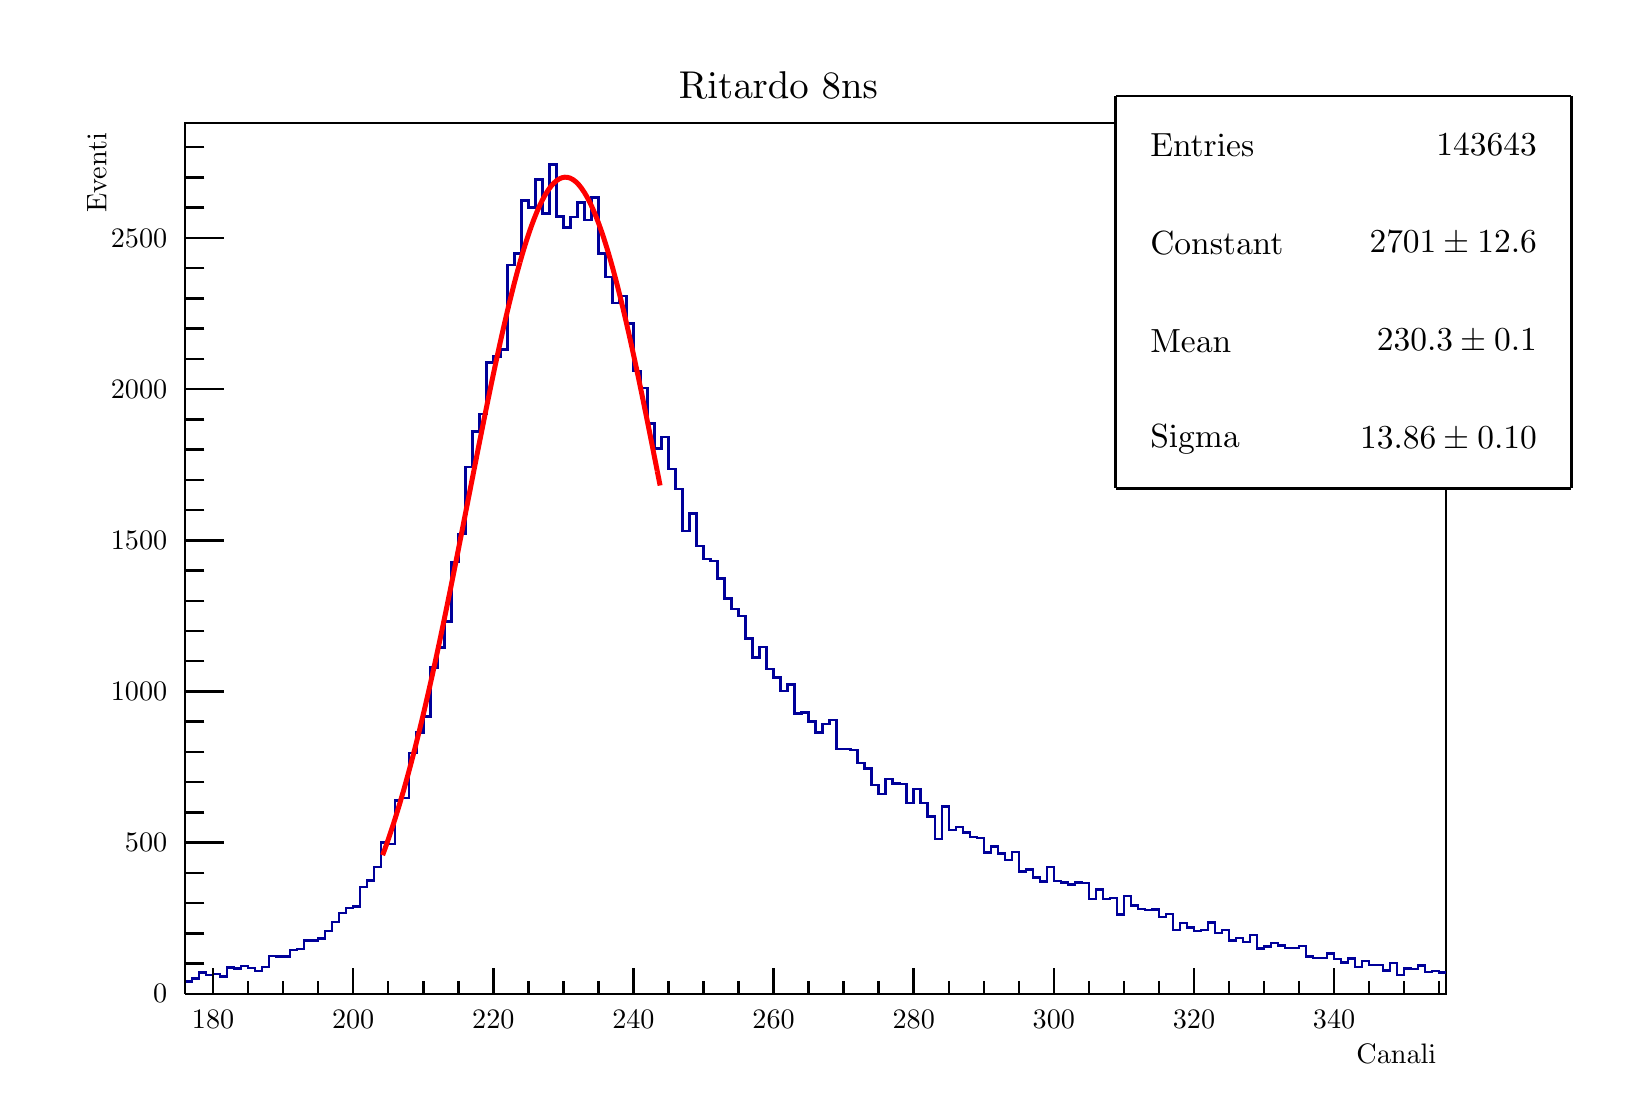
\begin{tikzpicture}
\pgfdeclareplotmark{cross} {
\pgfpathmoveto{\pgfpoint{-0.3\pgfplotmarksize}{\pgfplotmarksize}}
\pgfpathlineto{\pgfpoint{+0.3\pgfplotmarksize}{\pgfplotmarksize}}
\pgfpathlineto{\pgfpoint{+0.3\pgfplotmarksize}{0.3\pgfplotmarksize}}
\pgfpathlineto{\pgfpoint{+1\pgfplotmarksize}{0.3\pgfplotmarksize}}
\pgfpathlineto{\pgfpoint{+1\pgfplotmarksize}{-0.3\pgfplotmarksize}}
\pgfpathlineto{\pgfpoint{+0.3\pgfplotmarksize}{-0.3\pgfplotmarksize}}
\pgfpathlineto{\pgfpoint{+0.3\pgfplotmarksize}{-1.\pgfplotmarksize}}
\pgfpathlineto{\pgfpoint{-0.3\pgfplotmarksize}{-1.\pgfplotmarksize}}
\pgfpathlineto{\pgfpoint{-0.3\pgfplotmarksize}{-0.3\pgfplotmarksize}}
\pgfpathlineto{\pgfpoint{-1.\pgfplotmarksize}{-0.3\pgfplotmarksize}}
\pgfpathlineto{\pgfpoint{-1.\pgfplotmarksize}{0.3\pgfplotmarksize}}
\pgfpathlineto{\pgfpoint{-0.3\pgfplotmarksize}{0.3\pgfplotmarksize}}
\pgfpathclose
\pgfusepathqstroke
}
\pgfdeclareplotmark{cross*} {
\pgfpathmoveto{\pgfpoint{-0.3\pgfplotmarksize}{\pgfplotmarksize}}
\pgfpathlineto{\pgfpoint{+0.3\pgfplotmarksize}{\pgfplotmarksize}}
\pgfpathlineto{\pgfpoint{+0.3\pgfplotmarksize}{0.3\pgfplotmarksize}}
\pgfpathlineto{\pgfpoint{+1\pgfplotmarksize}{0.3\pgfplotmarksize}}
\pgfpathlineto{\pgfpoint{+1\pgfplotmarksize}{-0.3\pgfplotmarksize}}
\pgfpathlineto{\pgfpoint{+0.3\pgfplotmarksize}{-0.3\pgfplotmarksize}}
\pgfpathlineto{\pgfpoint{+0.3\pgfplotmarksize}{-1.\pgfplotmarksize}}
\pgfpathlineto{\pgfpoint{-0.3\pgfplotmarksize}{-1.\pgfplotmarksize}}
\pgfpathlineto{\pgfpoint{-0.3\pgfplotmarksize}{-0.3\pgfplotmarksize}}
\pgfpathlineto{\pgfpoint{-1.\pgfplotmarksize}{-0.3\pgfplotmarksize}}
\pgfpathlineto{\pgfpoint{-1.\pgfplotmarksize}{0.3\pgfplotmarksize}}
\pgfpathlineto{\pgfpoint{-0.3\pgfplotmarksize}{0.3\pgfplotmarksize}}
\pgfpathclose
\pgfusepathqfillstroke
}
\pgfdeclareplotmark{newstar} {
\pgfpathmoveto{\pgfqpoint{0pt}{\pgfplotmarksize}}
\pgfpathlineto{\pgfqpointpolar{44}{0.5\pgfplotmarksize}}
\pgfpathlineto{\pgfqpointpolar{18}{\pgfplotmarksize}}
\pgfpathlineto{\pgfqpointpolar{-20}{0.5\pgfplotmarksize}}
\pgfpathlineto{\pgfqpointpolar{-54}{\pgfplotmarksize}}
\pgfpathlineto{\pgfqpointpolar{-90}{0.5\pgfplotmarksize}}
\pgfpathlineto{\pgfqpointpolar{234}{\pgfplotmarksize}}
\pgfpathlineto{\pgfqpointpolar{198}{0.5\pgfplotmarksize}}
\pgfpathlineto{\pgfqpointpolar{162}{\pgfplotmarksize}}
\pgfpathlineto{\pgfqpointpolar{134}{0.5\pgfplotmarksize}}
\pgfpathclose
\pgfusepathqstroke
}
\pgfdeclareplotmark{newstar*} {
\pgfpathmoveto{\pgfqpoint{0pt}{\pgfplotmarksize}}
\pgfpathlineto{\pgfqpointpolar{44}{0.5\pgfplotmarksize}}
\pgfpathlineto{\pgfqpointpolar{18}{\pgfplotmarksize}}
\pgfpathlineto{\pgfqpointpolar{-20}{0.5\pgfplotmarksize}}
\pgfpathlineto{\pgfqpointpolar{-54}{\pgfplotmarksize}}
\pgfpathlineto{\pgfqpointpolar{-90}{0.5\pgfplotmarksize}}
\pgfpathlineto{\pgfqpointpolar{234}{\pgfplotmarksize}}
\pgfpathlineto{\pgfqpointpolar{198}{0.5\pgfplotmarksize}}
\pgfpathlineto{\pgfqpointpolar{162}{\pgfplotmarksize}}
\pgfpathlineto{\pgfqpointpolar{134}{0.5\pgfplotmarksize}}
\pgfpathclose
\pgfusepathqfillstroke
}
\definecolor{c}{rgb}{1,1,1};
\draw [color=c, fill=c] (0,0) rectangle (20,13.4957);
\draw [color=c, fill=c] (1.9914,1.23209) rectangle (18.0086,12.2923);
\definecolor{c}{rgb}{0,0,0};
\draw [c,line width=0.9] (1.9914,1.23209) -- (1.9914,12.2923) -- (18.0086,12.2923) -- (18.0086,1.23209) -- (1.9914,1.23209);
\definecolor{c}{rgb}{1,1,1};
\draw [color=c, fill=c] (1.9914,1.23209) rectangle (18.0086,12.2923);
\definecolor{c}{rgb}{0,0,0};
\draw [c,line width=0.9] (1.9914,1.23209) -- (1.9914,12.2923) -- (18.0086,12.2923) -- (18.0086,1.23209) -- (1.9914,1.23209);
\definecolor{c}{rgb}{0,0,0.6};
\draw [c,line width=0.9] (1.9914,1.38954) -- (2.08039,1.38954) -- (2.08039,1.42794) -- (2.16937,1.42794) -- (2.16937,1.5009) -- (2.25836,1.5009) -- (2.25836,1.47402) -- (2.34734,1.47402) -- (2.34734,1.48554) -- (2.43633,1.48554) -- (2.43633,1.45098)
 -- (2.52531,1.45098) -- (2.52531,1.57002) -- (2.61429,1.57002) -- (2.61429,1.55466) -- (2.70328,1.55466) -- (2.70328,1.58538) -- (2.79226,1.58538) -- (2.79226,1.56234) -- (2.88125,1.56234) -- (2.88125,1.52394) -- (2.97023,1.52394) --
 (2.97023,1.57386) -- (3.05922,1.57386) -- (3.05922,1.71595) -- (3.1482,1.71595) -- (3.1482,1.70443) -- (3.23719,1.70443) -- (3.23719,1.70827) -- (3.32617,1.70827) -- (3.32617,1.78891) -- (3.41515,1.78891) -- (3.41515,1.80043) -- (3.50414,1.80043) --
 (3.50414,1.9118) -- (3.59312,1.9118) -- (3.59312,1.9118) -- (3.68211,1.9118) -- (3.68211,1.93484) -- (3.77109,1.93484) -- (3.77109,2.03084) -- (3.86008,2.03084) -- (3.86008,2.14604) -- (3.94906,2.14604) -- (3.94906,2.26125) -- (4.03805,2.26125) --
 (4.03805,2.32269) -- (4.12703,2.32269) -- (4.12703,2.34189) -- (4.21601,2.34189) -- (4.21601,2.5915) -- (4.305,2.5915) -- (4.305,2.67214) -- (4.39398,2.67214) -- (4.39398,2.84495) -- (4.48297,2.84495) -- (4.48297,3.156) -- (4.57195,3.156) --
 (4.57195,3.13296) -- (4.66094,3.13296) -- (4.66094,3.68978) -- (4.74992,3.68978) -- (4.74992,3.7205) -- (4.8389,3.7205) -- (4.8389,4.29268) -- (4.92789,4.29268) -- (4.92789,4.55381) -- (5.01687,4.55381) -- (5.01687,4.75734) -- (5.10586,4.75734) --
 (5.10586,5.3756) -- (5.19484,5.3756) -- (5.19484,5.63289) -- (5.28383,5.63289) -- (5.28383,5.9593) -- (5.37281,5.9593) -- (5.37281,6.71581) -- (5.4618,6.71581) -- (5.4618,7.0691) -- (5.55078,7.0691) -- (5.55078,7.92545) -- (5.63976,7.92545) --
 (5.63976,8.37475) -- (5.72875,8.37475) -- (5.72875,8.59748) -- (5.81773,8.59748) -- (5.81773,9.2503) -- (5.90672,9.2503) -- (5.90672,9.3271) -- (5.9957,9.3271) -- (5.9957,9.41542) -- (6.08469,9.41542) -- (6.08469,10.4868) -- (6.17367,10.4868) --
 (6.17367,10.6366) -- (6.26266,10.6366) -- (6.26266,11.3048) -- (6.35164,11.3048) -- (6.35164,11.2203) -- (6.44062,11.2203) -- (6.44062,11.5736) -- (6.52961,11.5736) -- (6.52961,11.1396) -- (6.61859,11.1396) -- (6.61859,11.7656) -- (6.70758,11.7656)
 -- (6.70758,11.1051) -- (6.79656,11.1051) -- (6.79656,10.963) -- (6.88555,10.963) -- (6.88555,11.1012) -- (6.97453,11.1012) -- (6.97453,11.2817) -- (7.06351,11.2817) -- (7.06351,11.059) -- (7.1525,11.059) -- (7.1525,11.347) -- (7.24148,11.347) --
 (7.24148,10.6366) -- (7.33047,10.6366) -- (7.33047,10.3371) -- (7.41945,10.3371) -- (7.41945,10.0068) -- (7.50844,10.0068) -- (7.50844,10.0951) -- (7.59742,10.0951) -- (7.59742,9.74568) -- (7.68641,9.74568) -- (7.68641,9.14277) -- (7.77539,9.14277)
 -- (7.77539,8.92389) -- (7.86437,8.92389) -- (7.86437,8.47459) -- (7.95336,8.47459) -- (7.95336,8.1597) -- (8.04234,8.1597) -- (8.04234,8.30178) -- (8.13133,8.30178) -- (8.13133,7.89857) -- (8.22031,7.89857) -- (8.22031,7.64512) -- (8.3093,7.64512)
 -- (8.3093,7.1075) -- (8.39828,7.1075) -- (8.39828,7.33023) -- (8.48727,7.33023) -- (8.48727,6.91934) -- (8.57625,6.91934) -- (8.57625,6.75421) -- (8.66523,6.75421) -- (8.66523,6.72733) -- (8.75422,6.72733) -- (8.75422,6.50844) -- (8.8432,6.50844)
 -- (8.8432,6.25115) -- (8.93219,6.25115) -- (8.93219,6.12059) -- (9.02117,6.12059) -- (9.02117,6.03226) -- (9.11016,6.03226) -- (9.11016,5.74425) -- (9.19914,5.74425) -- (9.19914,5.50232) -- (9.28813,5.50232) -- (9.28813,5.63673) --
 (9.37711,5.63673) -- (9.37711,5.36024) -- (9.46609,5.36024) -- (9.46609,5.24888) -- (9.55508,5.24888) -- (9.55508,5.07607) -- (9.64406,5.07607) -- (9.64406,5.16055) -- (9.73305,5.16055) -- (9.73305,4.7919) -- (9.82203,4.7919) -- (9.82203,4.80342) --
 (9.91102,4.80342) -- (9.91102,4.68822) -- (10,4.68822) -- (10,4.54997) -- (10.089,4.54997) -- (10.089,4.66133) -- (10.178,4.66133) -- (10.178,4.71126) -- (10.267,4.71126) -- (10.267,4.33876) -- (10.3559,4.33876) -- (10.3559,4.3426) --
 (10.4449,4.3426) -- (10.4449,4.32724) -- (10.5339,4.32724) -- (10.5339,4.16212) -- (10.6229,4.16212) -- (10.6229,4.09299) -- (10.7119,4.09299) -- (10.7119,3.88179) -- (10.8009,3.88179) -- (10.8009,3.77042) -- (10.8898,3.77042) -- (10.8898,3.96243)
 -- (10.9788,3.96243) -- (10.9788,3.90099) -- (11.0678,3.90099) -- (11.0678,3.89715) -- (11.1568,3.89715) -- (11.1568,3.65522) -- (11.2458,3.65522) -- (11.2458,3.8357) -- (11.3348,3.8357) -- (11.3348,3.65906) -- (11.4237,3.65906) -- (11.4237,3.48625)
 -- (11.5127,3.48625) -- (11.5127,3.19824) -- (11.6017,3.19824) -- (11.6017,3.61298) -- (11.6907,3.61298) -- (11.6907,3.31345) -- (11.7797,3.31345) -- (11.7797,3.35185) -- (11.8687,3.35185) -- (11.8687,3.28273) -- (11.9577,3.28273) --
 (11.9577,3.22128) -- (12.0466,3.22128) -- (12.0466,3.2136) -- (12.1356,3.2136) -- (12.1356,3.02544) -- (12.2246,3.02544) -- (12.2246,3.10224) -- (12.3136,3.10224) -- (12.3136,3.01776) -- (12.4026,3.01776) -- (12.4026,2.93327) -- (12.4916,2.93327) --
 (12.4916,3.03696) -- (12.5805,3.03696) -- (12.5805,2.78735) -- (12.6695,2.78735) -- (12.6695,2.81039) -- (12.7585,2.81039) -- (12.7585,2.71054) -- (12.8475,2.71054) -- (12.8475,2.65678) -- (12.9365,2.65678) -- (12.9365,2.84495) -- (13.0255,2.84495)
 -- (13.0255,2.6683) -- (13.1145,2.6683) -- (13.1145,2.6491) -- (13.2034,2.6491) -- (13.2034,2.61838) -- (13.2924,2.61838) -- (13.2924,2.64526) -- (13.3814,2.64526) -- (13.3814,2.63758) -- (13.4704,2.63758) -- (13.4704,2.43405) -- (13.5594,2.43405)
 -- (13.5594,2.55694) -- (13.6484,2.55694) -- (13.6484,2.43405) -- (13.7373,2.43405) -- (13.7373,2.44942) -- (13.8263,2.44942) -- (13.8263,2.23821) -- (13.9153,2.23821) -- (13.9153,2.47246) -- (14.0043,2.47246) -- (14.0043,2.35725) --
 (14.0933,2.35725) -- (14.0933,2.31117) -- (14.1823,2.31117) -- (14.1823,2.29965) -- (14.2713,2.29965) -- (14.2713,2.30349) -- (14.3602,2.30349) -- (14.3602,2.21133) -- (14.4492,2.21133) -- (14.4492,2.24589) -- (14.5382,2.24589) -- (14.5382,2.0462)
 -- (14.6272,2.0462) -- (14.6272,2.13068) -- (14.7162,2.13068) -- (14.7162,2.07692) -- (14.8052,2.07692) -- (14.8052,2.03084) -- (14.8941,2.03084) -- (14.8941,2.0462) -- (14.9831,2.0462) -- (14.9831,2.13836) -- (15.0721,2.13836) -- (15.0721,2.0078)
 -- (15.1611,2.0078) -- (15.1611,2.0462) -- (15.2501,2.0462) -- (15.2501,1.90796) -- (15.3391,1.90796) -- (15.3391,1.94252) -- (15.428,1.94252) -- (15.428,1.8926) -- (15.517,1.8926) -- (15.517,1.98092) -- (15.606,1.98092) -- (15.606,1.80811) --
 (15.695,1.80811) -- (15.695,1.83115) -- (15.784,1.83115) -- (15.784,1.88107) -- (15.873,1.88107) -- (15.873,1.84651) -- (15.962,1.84651) -- (15.962,1.81195) -- (16.0509,1.81195) -- (16.0509,1.81579) -- (16.1399,1.81579) -- (16.1399,1.84267) --
 (16.2289,1.84267) -- (16.2289,1.70443) -- (16.3179,1.70443) -- (16.3179,1.68523) -- (16.4069,1.68523) -- (16.4069,1.68523) -- (16.4959,1.68523) -- (16.4959,1.74283) -- (16.5848,1.74283) -- (16.5848,1.67371) -- (16.6738,1.67371) -- (16.6738,1.63147)
 -- (16.7628,1.63147) -- (16.7628,1.68139) -- (16.8518,1.68139) -- (16.8518,1.57386) -- (16.9408,1.57386) -- (16.9408,1.64683) -- (17.0298,1.64683) -- (17.0298,1.5969) -- (17.1188,1.5969) -- (17.1188,1.60074) -- (17.2077,1.60074) -- (17.2077,1.52778)
 -- (17.2967,1.52778) -- (17.2967,1.62379) -- (17.3857,1.62379) -- (17.3857,1.47018) -- (17.4747,1.47018) -- (17.4747,1.55466) -- (17.5637,1.55466) -- (17.5637,1.55082) -- (17.6527,1.55082) -- (17.6527,1.58922) -- (17.7416,1.58922) --
 (17.7416,1.51242) -- (17.8306,1.51242) -- (17.8306,1.5201) -- (17.9196,1.5201) -- (17.9196,1.50474) -- (18.0086,1.50474);
\definecolor{c}{rgb}{1,1,1};
\draw [color=c, fill=c] (13.8109,7.65043) rectangle (19.5989,12.6361);
\definecolor{c}{rgb}{0,0,0};
\draw [c,line width=0.9] (13.8109,7.65043) -- (19.5989,7.65043);
\draw [c,line width=0.9] (19.5989,7.65043) -- (19.5989,12.6361);
\draw [c,line width=0.9] (19.5989,12.6361) -- (13.8109,12.6361);
\draw [c,line width=0.9] (13.8109,12.6361) -- (13.8109,7.65043);
\draw [anchor= west] (14.1003,12.0129) node[scale=1.20912, color=c, rotate=0]{Entries };
\draw [anchor= east] (19.3095,12.0129) node[scale=1.20912, color=c, rotate=0]{ 143643};
\draw [anchor= west] (14.1003,10.7665) node[scale=1.20912, color=c, rotate=0]{Constant };
\draw [anchor= east] (19.3095,10.7665) node[scale=1.20912, color=c, rotate=0]{$  2701 \pm 12.6$};
\draw [anchor= west] (14.1003,9.52006) node[scale=1.20912, color=c, rotate=0]{Mean     };
\draw [anchor= east] (19.3095,9.52006) node[scale=1.20912, color=c, rotate=0]{$ 230.3 \pm 0.1$};
\draw [anchor= west] (14.1003,8.27364) node[scale=1.20912, color=c, rotate=0]{Sigma    };
\draw [anchor= east] (19.3095,8.27364) node[scale=1.20912, color=c, rotate=0]{$ 13.86 \pm 0.10$};
\definecolor{c}{rgb}{1,0,0};
\draw [c,line width=1.8] (4.50076,2.99334) -- (4.53636,3.09092) -- (4.57195,3.19228) -- (4.60755,3.29744) -- (4.64314,3.40642) -- (4.67873,3.51926) -- (4.71433,3.63595) -- (4.74992,3.75649) -- (4.78551,3.88087) -- (4.82111,4.00906) --
 (4.8567,4.14103) -- (4.8923,4.27674) -- (4.92789,4.41613) -- (4.96348,4.55912) -- (4.99908,4.70565) -- (5.03467,4.85561) -- (5.07026,5.0089) -- (5.10586,5.16539) -- (5.14145,5.32496) -- (5.17705,5.48746) -- (5.21264,5.65273) -- (5.24823,5.82059) --
 (5.28383,5.99087) -- (5.31942,6.16335) -- (5.35501,6.33784) -- (5.39061,6.51409) -- (5.4262,6.69189) -- (5.4618,6.87097) -- (5.49739,7.05108) -- (5.53298,7.23194) -- (5.56858,7.41327) -- (5.60417,7.59479) -- (5.63976,7.77618) -- (5.67536,7.95714) --
 (5.71095,8.13736) -- (5.74655,8.3165) -- (5.78214,8.49424) -- (5.81773,8.67024) -- (5.85333,8.84416) -- (5.88892,9.01567) -- (5.92451,9.18442) -- (5.96011,9.35007) -- (5.9957,9.51226) -- (6.0313,9.67067) -- (6.06689,9.82495) -- (6.10248,9.97477) --
 (6.13808,10.1198) -- (6.17367,10.2597) -- (6.20926,10.3942) -- (6.24486,10.5229);
\draw [c,line width=1.8] (6.24486,10.5229) -- (6.28045,10.6456) -- (6.31605,10.762) -- (6.35164,10.8718) -- (6.38723,10.9748) -- (6.42283,11.0707) -- (6.45842,11.1592) -- (6.49401,11.2402) -- (6.52961,11.3134) -- (6.5652,11.3788) -- (6.6008,11.436)
 -- (6.63639,11.4851) -- (6.67198,11.5258) -- (6.70758,11.558) -- (6.74317,11.5818) -- (6.77876,11.5969) -- (6.81436,11.6035) -- (6.84995,11.6014) -- (6.88555,11.5906) -- (6.92114,11.5713) -- (6.95673,11.5434) -- (6.99233,11.5071) --
 (7.02792,11.4623) -- (7.06351,11.4093) -- (7.09911,11.3481) -- (7.1347,11.2789) -- (7.1703,11.2019) -- (7.20589,11.1172) -- (7.24148,11.0251) -- (7.27708,10.9258) -- (7.31267,10.8195) -- (7.34826,10.7065) -- (7.38386,10.587) -- (7.41945,10.4613) --
 (7.45505,10.3297) -- (7.49064,10.1926) -- (7.52623,10.0501) -- (7.56183,9.90276) -- (7.59742,9.75073) -- (7.63302,9.59441) -- (7.66861,9.43412) -- (7.7042,9.27021) -- (7.7398,9.10302) -- (7.77539,8.93289) -- (7.81098,8.76017) -- (7.84658,8.5852) --
 (7.88217,8.40831) -- (7.91777,8.22985) -- (7.95336,8.05015) -- (7.98895,7.86953);
\draw [c,line width=1.8] (7.98895,7.86953) -- (8.02455,7.68832);
\definecolor{c}{rgb}{0,0,0};
\draw [c,line width=0.9] (1.9914,1.23209) -- (18.0086,1.23209);
\draw [anchor= east] (18.0086,0.476332) node[scale=1.01821, color=c, rotate=0]{Canali};
\draw [c,line width=0.9] (2.34734,1.55634) -- (2.34734,1.23209);
\draw [c,line width=0.9] (2.79226,1.39421) -- (2.79226,1.23209);
\draw [c,line width=0.9] (3.23719,1.39421) -- (3.23719,1.23209);
\draw [c,line width=0.9] (3.68211,1.39421) -- (3.68211,1.23209);
\draw [c,line width=0.9] (4.12703,1.55634) -- (4.12703,1.23209);
\draw [c,line width=0.9] (4.57195,1.39421) -- (4.57195,1.23209);
\draw [c,line width=0.9] (5.01687,1.39421) -- (5.01687,1.23209);
\draw [c,line width=0.9] (5.4618,1.39421) -- (5.4618,1.23209);
\draw [c,line width=0.9] (5.90672,1.55634) -- (5.90672,1.23209);
\draw [c,line width=0.9] (6.35164,1.39421) -- (6.35164,1.23209);
\draw [c,line width=0.9] (6.79656,1.39421) -- (6.79656,1.23209);
\draw [c,line width=0.9] (7.24148,1.39421) -- (7.24148,1.23209);
\draw [c,line width=0.9] (7.68641,1.55634) -- (7.68641,1.23209);
\draw [c,line width=0.9] (8.13133,1.39421) -- (8.13133,1.23209);
\draw [c,line width=0.9] (8.57625,1.39421) -- (8.57625,1.23209);
\draw [c,line width=0.9] (9.02117,1.39421) -- (9.02117,1.23209);
\draw [c,line width=0.9] (9.46609,1.55634) -- (9.46609,1.23209);
\draw [c,line width=0.9] (9.91102,1.39421) -- (9.91102,1.23209);
\draw [c,line width=0.9] (10.3559,1.39421) -- (10.3559,1.23209);
\draw [c,line width=0.9] (10.8009,1.39421) -- (10.8009,1.23209);
\draw [c,line width=0.9] (11.2458,1.55634) -- (11.2458,1.23209);
\draw [c,line width=0.9] (11.6907,1.39421) -- (11.6907,1.23209);
\draw [c,line width=0.9] (12.1356,1.39421) -- (12.1356,1.23209);
\draw [c,line width=0.9] (12.5805,1.39421) -- (12.5805,1.23209);
\draw [c,line width=0.9] (13.0255,1.55634) -- (13.0255,1.23209);
\draw [c,line width=0.9] (13.4704,1.39421) -- (13.4704,1.23209);
\draw [c,line width=0.9] (13.9153,1.39421) -- (13.9153,1.23209);
\draw [c,line width=0.9] (14.3602,1.39421) -- (14.3602,1.23209);
\draw [c,line width=0.9] (14.8052,1.55634) -- (14.8052,1.23209);
\draw [c,line width=0.9] (15.2501,1.39421) -- (15.2501,1.23209);
\draw [c,line width=0.9] (15.695,1.39421) -- (15.695,1.23209);
\draw [c,line width=0.9] (16.1399,1.39421) -- (16.1399,1.23209);
\draw [c,line width=0.9] (16.5848,1.55634) -- (16.5848,1.23209);
\draw [c,line width=0.9] (2.34734,1.55634) -- (2.34734,1.23209);
\draw [c,line width=0.9] (16.5848,1.55634) -- (16.5848,1.23209);
\draw [c,line width=0.9] (17.0298,1.39421) -- (17.0298,1.23209);
\draw [c,line width=0.9] (17.4747,1.39421) -- (17.4747,1.23209);
\draw [c,line width=0.9] (17.9196,1.39421) -- (17.9196,1.23209);
\draw [anchor=base] (2.34734,0.786734) node[scale=1.01821, color=c, rotate=0]{180};
\draw [anchor=base] (4.12703,0.786734) node[scale=1.01821, color=c, rotate=0]{200};
\draw [anchor=base] (5.90672,0.786734) node[scale=1.01821, color=c, rotate=0]{220};
\draw [anchor=base] (7.68641,0.786734) node[scale=1.01821, color=c, rotate=0]{240};
\draw [anchor=base] (9.46609,0.786734) node[scale=1.01821, color=c, rotate=0]{260};
\draw [anchor=base] (11.2458,0.786734) node[scale=1.01821, color=c, rotate=0]{280};
\draw [anchor=base] (13.0255,0.786734) node[scale=1.01821, color=c, rotate=0]{300};
\draw [anchor=base] (14.8052,0.786734) node[scale=1.01821, color=c, rotate=0]{320};
\draw [anchor=base] (16.5848,0.786734) node[scale=1.01821, color=c, rotate=0]{340};
\draw [c,line width=0.9] (1.9914,1.23209) -- (1.9914,12.2923);
\draw [anchor= east] (0.871404,12.2923) node[scale=1.01821, color=c, rotate=90]{Eventi};
\draw [c,line width=0.9] (2.48312,1.23209) -- (1.9914,1.23209);
\draw [c,line width=0.9] (2.23726,1.61611) -- (1.9914,1.61611);
\draw [c,line width=0.9] (2.23726,2.00012) -- (1.9914,2.00012);
\draw [c,line width=0.9] (2.23726,2.38413) -- (1.9914,2.38413);
\draw [c,line width=0.9] (2.23726,2.76815) -- (1.9914,2.76815);
\draw [c,line width=0.9] (2.48312,3.15216) -- (1.9914,3.15216);
\draw [c,line width=0.9] (2.23726,3.53617) -- (1.9914,3.53617);
\draw [c,line width=0.9] (2.23726,3.92019) -- (1.9914,3.92019);
\draw [c,line width=0.9] (2.23726,4.3042) -- (1.9914,4.3042);
\draw [c,line width=0.9] (2.23726,4.68822) -- (1.9914,4.68822);
\draw [c,line width=0.9] (2.48312,5.07223) -- (1.9914,5.07223);
\draw [c,line width=0.9] (2.23726,5.45624) -- (1.9914,5.45624);
\draw [c,line width=0.9] (2.23726,5.84026) -- (1.9914,5.84026);
\draw [c,line width=0.9] (2.23726,6.22427) -- (1.9914,6.22427);
\draw [c,line width=0.9] (2.23726,6.60828) -- (1.9914,6.60828);
\draw [c,line width=0.9] (2.48312,6.9923) -- (1.9914,6.9923);
\draw [c,line width=0.9] (2.23726,7.37631) -- (1.9914,7.37631);
\draw [c,line width=0.9] (2.23726,7.76033) -- (1.9914,7.76033);
\draw [c,line width=0.9] (2.23726,8.14434) -- (1.9914,8.14434);
\draw [c,line width=0.9] (2.23726,8.52835) -- (1.9914,8.52835);
\draw [c,line width=0.9] (2.48312,8.91237) -- (1.9914,8.91237);
\draw [c,line width=0.9] (2.23726,9.29638) -- (1.9914,9.29638);
\draw [c,line width=0.9] (2.23726,9.68039) -- (1.9914,9.68039);
\draw [c,line width=0.9] (2.23726,10.0644) -- (1.9914,10.0644);
\draw [c,line width=0.9] (2.23726,10.4484) -- (1.9914,10.4484);
\draw [c,line width=0.9] (2.48312,10.8324) -- (1.9914,10.8324);
\draw [c,line width=0.9] (2.48312,10.8324) -- (1.9914,10.8324);
\draw [c,line width=0.9] (2.23726,11.2164) -- (1.9914,11.2164);
\draw [c,line width=0.9] (2.23726,11.6005) -- (1.9914,11.6005);
\draw [c,line width=0.9] (2.23726,11.9845) -- (1.9914,11.9845);
\draw [anchor= east] (1.8914,1.23209) node[scale=1.01821, color=c, rotate=0]{0};
\draw [anchor= east] (1.8914,3.15216) node[scale=1.01821, color=c, rotate=0]{500};
\draw [anchor= east] (1.8914,5.07223) node[scale=1.01821, color=c, rotate=0]{1000};
\draw [anchor= east] (1.8914,6.9923) node[scale=1.01821, color=c, rotate=0]{1500};
\draw [anchor= east] (1.8914,8.91237) node[scale=1.01821, color=c, rotate=0]{2000};
\draw [anchor= east] (1.8914,10.8324) node[scale=1.01821, color=c, rotate=0]{2500};
\definecolor{c}{rgb}{1,1,1};
\draw [color=c, fill=c] (13.8109,7.65043) rectangle (19.5989,12.6361);
\definecolor{c}{rgb}{0,0,0};
\draw [c,line width=0.9] (13.8109,7.65043) -- (19.5989,7.65043);
\draw [c,line width=0.9] (19.5989,7.65043) -- (19.5989,12.6361);
\draw [c,line width=0.9] (19.5989,12.6361) -- (13.8109,12.6361);
\draw [c,line width=0.9] (13.8109,12.6361) -- (13.8109,7.65043);
\draw [anchor= west] (14.1003,12.0129) node[scale=1.20912, color=c, rotate=0]{Entries };
\draw [anchor= east] (19.3095,12.0129) node[scale=1.20912, color=c, rotate=0]{ 143643};
\draw [anchor= west] (14.1003,10.7665) node[scale=1.20912, color=c, rotate=0]{Constant };
\draw [anchor= east] (19.3095,10.7665) node[scale=1.20912, color=c, rotate=0]{$  2701 \pm 12.6$};
\draw [anchor= west] (14.1003,9.52006) node[scale=1.20912, color=c, rotate=0]{Mean     };
\draw [anchor= east] (19.3095,9.52006) node[scale=1.20912, color=c, rotate=0]{$ 230.3 \pm 0.1$};
\draw [anchor= west] (14.1003,8.27364) node[scale=1.20912, color=c, rotate=0]{Sigma    };
\draw [anchor= east] (19.3095,8.27364) node[scale=1.20912, color=c, rotate=0]{$ 13.86 \pm 0.10$};
\draw (9.52722,12.7794) node[scale=1.40004, color=c, rotate=0]{Ritardo 8ns};
\end{tikzpicture}

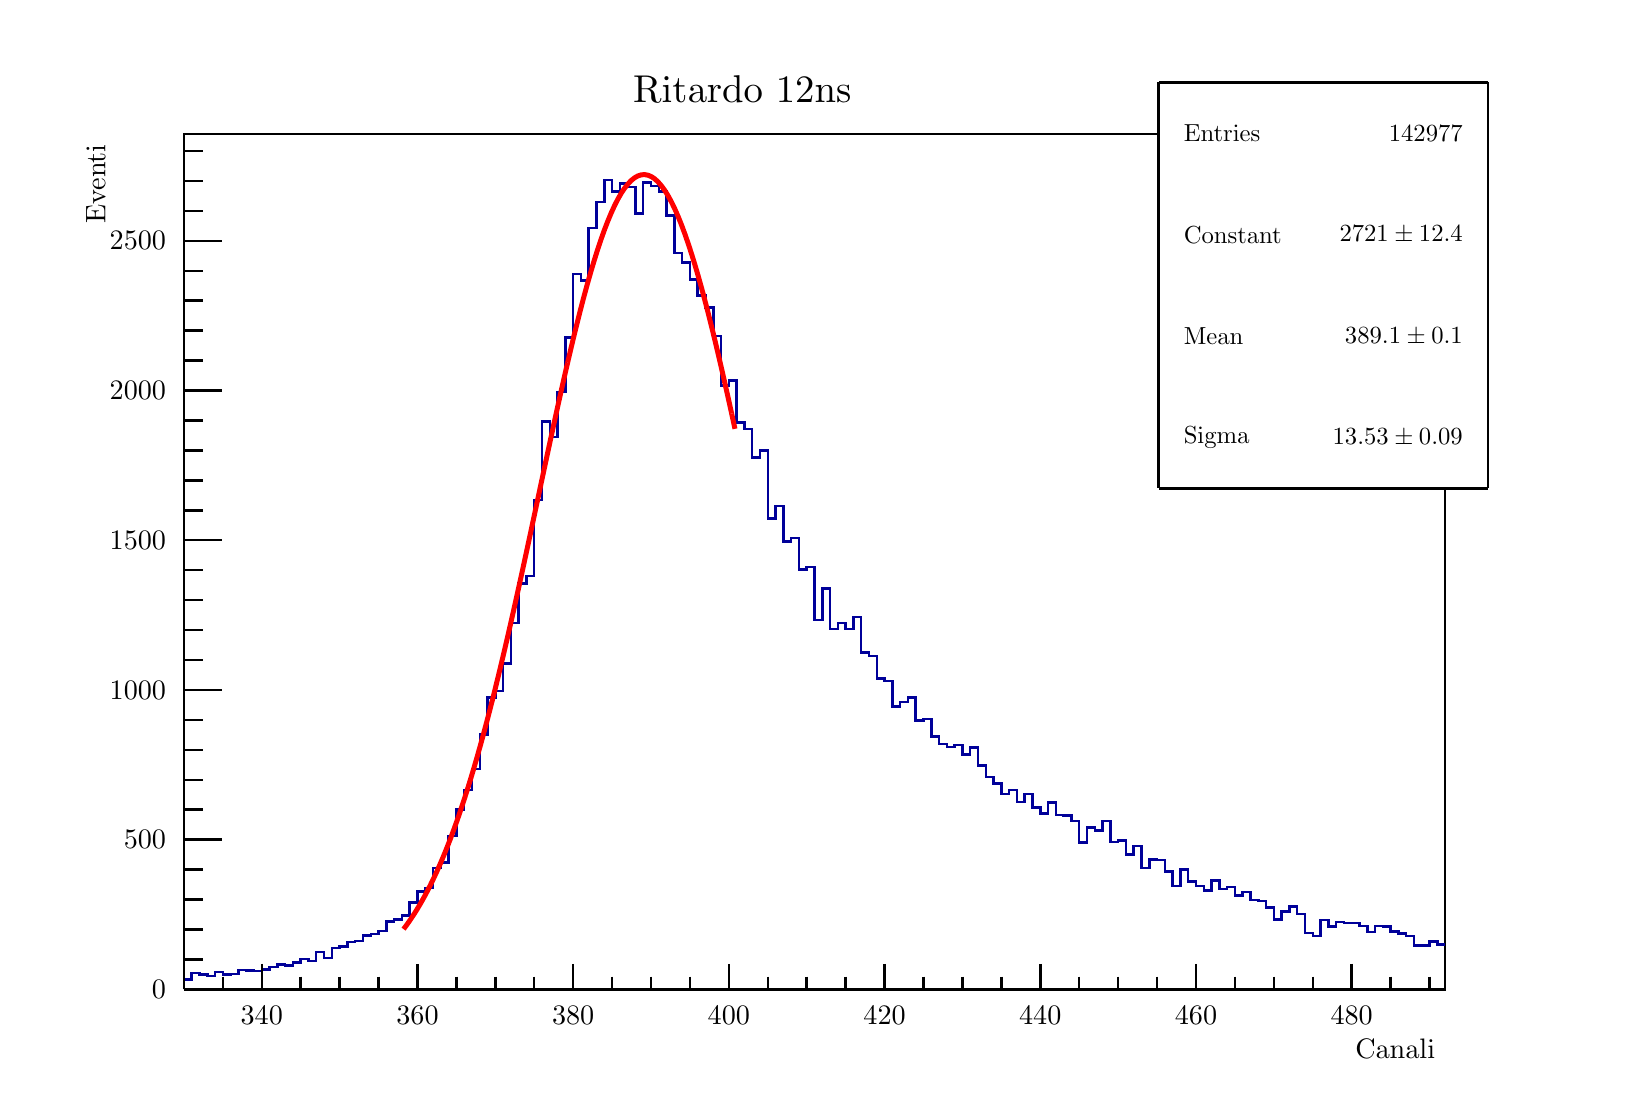
\begin{tikzpicture}
\pgfdeclareplotmark{cross} {
\pgfpathmoveto{\pgfpoint{-0.3\pgfplotmarksize}{\pgfplotmarksize}}
\pgfpathlineto{\pgfpoint{+0.3\pgfplotmarksize}{\pgfplotmarksize}}
\pgfpathlineto{\pgfpoint{+0.3\pgfplotmarksize}{0.3\pgfplotmarksize}}
\pgfpathlineto{\pgfpoint{+1\pgfplotmarksize}{0.3\pgfplotmarksize}}
\pgfpathlineto{\pgfpoint{+1\pgfplotmarksize}{-0.3\pgfplotmarksize}}
\pgfpathlineto{\pgfpoint{+0.3\pgfplotmarksize}{-0.3\pgfplotmarksize}}
\pgfpathlineto{\pgfpoint{+0.3\pgfplotmarksize}{-1.\pgfplotmarksize}}
\pgfpathlineto{\pgfpoint{-0.3\pgfplotmarksize}{-1.\pgfplotmarksize}}
\pgfpathlineto{\pgfpoint{-0.3\pgfplotmarksize}{-0.3\pgfplotmarksize}}
\pgfpathlineto{\pgfpoint{-1.\pgfplotmarksize}{-0.3\pgfplotmarksize}}
\pgfpathlineto{\pgfpoint{-1.\pgfplotmarksize}{0.3\pgfplotmarksize}}
\pgfpathlineto{\pgfpoint{-0.3\pgfplotmarksize}{0.3\pgfplotmarksize}}
\pgfpathclose
\pgfusepathqstroke
}
\pgfdeclareplotmark{cross*} {
\pgfpathmoveto{\pgfpoint{-0.3\pgfplotmarksize}{\pgfplotmarksize}}
\pgfpathlineto{\pgfpoint{+0.3\pgfplotmarksize}{\pgfplotmarksize}}
\pgfpathlineto{\pgfpoint{+0.3\pgfplotmarksize}{0.3\pgfplotmarksize}}
\pgfpathlineto{\pgfpoint{+1\pgfplotmarksize}{0.3\pgfplotmarksize}}
\pgfpathlineto{\pgfpoint{+1\pgfplotmarksize}{-0.3\pgfplotmarksize}}
\pgfpathlineto{\pgfpoint{+0.3\pgfplotmarksize}{-0.3\pgfplotmarksize}}
\pgfpathlineto{\pgfpoint{+0.3\pgfplotmarksize}{-1.\pgfplotmarksize}}
\pgfpathlineto{\pgfpoint{-0.3\pgfplotmarksize}{-1.\pgfplotmarksize}}
\pgfpathlineto{\pgfpoint{-0.3\pgfplotmarksize}{-0.3\pgfplotmarksize}}
\pgfpathlineto{\pgfpoint{-1.\pgfplotmarksize}{-0.3\pgfplotmarksize}}
\pgfpathlineto{\pgfpoint{-1.\pgfplotmarksize}{0.3\pgfplotmarksize}}
\pgfpathlineto{\pgfpoint{-0.3\pgfplotmarksize}{0.3\pgfplotmarksize}}
\pgfpathclose
\pgfusepathqfillstroke
}
\pgfdeclareplotmark{newstar} {
\pgfpathmoveto{\pgfqpoint{0pt}{\pgfplotmarksize}}
\pgfpathlineto{\pgfqpointpolar{44}{0.5\pgfplotmarksize}}
\pgfpathlineto{\pgfqpointpolar{18}{\pgfplotmarksize}}
\pgfpathlineto{\pgfqpointpolar{-20}{0.5\pgfplotmarksize}}
\pgfpathlineto{\pgfqpointpolar{-54}{\pgfplotmarksize}}
\pgfpathlineto{\pgfqpointpolar{-90}{0.5\pgfplotmarksize}}
\pgfpathlineto{\pgfqpointpolar{234}{\pgfplotmarksize}}
\pgfpathlineto{\pgfqpointpolar{198}{0.5\pgfplotmarksize}}
\pgfpathlineto{\pgfqpointpolar{162}{\pgfplotmarksize}}
\pgfpathlineto{\pgfqpointpolar{134}{0.5\pgfplotmarksize}}
\pgfpathclose
\pgfusepathqstroke
}
\pgfdeclareplotmark{newstar*} {
\pgfpathmoveto{\pgfqpoint{0pt}{\pgfplotmarksize}}
\pgfpathlineto{\pgfqpointpolar{44}{0.5\pgfplotmarksize}}
\pgfpathlineto{\pgfqpointpolar{18}{\pgfplotmarksize}}
\pgfpathlineto{\pgfqpointpolar{-20}{0.5\pgfplotmarksize}}
\pgfpathlineto{\pgfqpointpolar{-54}{\pgfplotmarksize}}
\pgfpathlineto{\pgfqpointpolar{-90}{0.5\pgfplotmarksize}}
\pgfpathlineto{\pgfqpointpolar{234}{\pgfplotmarksize}}
\pgfpathlineto{\pgfqpointpolar{198}{0.5\pgfplotmarksize}}
\pgfpathlineto{\pgfqpointpolar{162}{\pgfplotmarksize}}
\pgfpathlineto{\pgfqpointpolar{134}{0.5\pgfplotmarksize}}
\pgfpathclose
\pgfusepathqfillstroke
}
\definecolor{c}{rgb}{1,1,1};
\draw [color=c, fill=c] (0,0) rectangle (20,13.4957);
\draw [color=c, fill=c] (1.97708,1.2894) rectangle (17.9943,12.149);
\definecolor{c}{rgb}{0,0,0};
\draw [c,line width=0.9] (1.97708,1.2894) -- (1.97708,12.149) -- (17.9943,12.149) -- (17.9943,1.2894) -- (1.97708,1.2894);
\definecolor{c}{rgb}{1,1,1};
\draw [color=c, fill=c] (1.97708,1.2894) rectangle (17.9943,12.149);
\definecolor{c}{rgb}{0,0,0};
\draw [c,line width=0.9] (1.97708,1.2894) -- (1.97708,12.149) -- (17.9943,12.149) -- (17.9943,1.2894) -- (1.97708,1.2894);
\definecolor{c}{rgb}{0,0,0.6};
\draw [c,line width=0.9] (1.97708,1.41488) -- (2.07595,1.41488) -- (2.07595,1.49854) -- (2.17482,1.49854) -- (2.17482,1.47952) -- (2.27369,1.47952) -- (2.27369,1.45671) -- (2.37256,1.45671) -- (2.37256,1.50994) -- (2.47144,1.50994) --
 (2.47144,1.47572) -- (2.57031,1.47572) -- (2.57031,1.48713) -- (2.66918,1.48713) -- (2.66918,1.53276) -- (2.76805,1.53276) -- (2.76805,1.52896) -- (2.86692,1.52896) -- (2.86692,1.52135) -- (2.96579,1.52135) -- (2.96579,1.54036) -- (3.06466,1.54036)
 -- (3.06466,1.57078) -- (3.16354,1.57078) -- (3.16354,1.60501) -- (3.26241,1.60501) -- (3.26241,1.5898) -- (3.36128,1.5898) -- (3.36128,1.62782) -- (3.46015,1.62782) -- (3.46015,1.67345) -- (3.55902,1.67345) -- (3.55902,1.64683) -- (3.65789,1.64683)
 -- (3.65789,1.76091) -- (3.75677,1.76091) -- (3.75677,1.68866) -- (3.85564,1.68866) -- (3.85564,1.81415) -- (3.95451,1.81415) -- (3.95451,1.83316) -- (4.05338,1.83316) -- (4.05338,1.8902) -- (4.15225,1.8902) -- (4.15225,1.90541) -- (4.25112,1.90541)
 -- (4.25112,1.97385) -- (4.34999,1.97385) -- (4.34999,1.99286) -- (4.44887,1.99286) -- (4.44887,2.03089) -- (4.54774,2.03089) -- (4.54774,2.15257) -- (4.64661,2.15257) -- (4.64661,2.17919) -- (4.74548,2.17919) -- (4.74548,2.22862) --
 (4.84435,2.22862) -- (4.84435,2.39213) -- (4.94322,2.39213) -- (4.94322,2.53282) -- (5.0421,2.53282) -- (5.0421,2.57465) -- (5.14097,2.57465) -- (5.14097,2.83322) -- (5.23984,2.83322) -- (5.23984,2.89786) -- (5.33871,2.89786) -- (5.33871,3.24009) --
 (5.43758,3.24009) -- (5.43758,3.57091) -- (5.53645,3.57091) -- (5.53645,3.82187) -- (5.63532,3.82187) -- (5.63532,4.08805) -- (5.7342,4.08805) -- (5.7342,4.52534) -- (5.83307,4.52534) -- (5.83307,4.99305) -- (5.93194,4.99305) -- (5.93194,5.0767) --
 (6.03081,5.0767) -- (6.03081,5.42653) -- (6.12968,5.42653) -- (6.12968,5.94368) -- (6.22855,5.94368) -- (6.22855,6.44561) -- (6.32743,6.44561) -- (6.32743,6.54067) -- (6.4263,6.54067) -- (6.4263,7.50271) -- (6.52517,7.50271) -- (6.52517,8.49897) --
 (6.62404,8.49897) -- (6.62404,8.30124) -- (6.72291,8.30124) -- (6.72291,8.87542) -- (6.82178,8.87542) -- (6.82178,9.56747) -- (6.92066,9.56747) -- (6.92066,10.3774) -- (7.01953,10.3774) -- (7.01953,10.2938) -- (7.1184,10.2938) -- (7.1184,10.9592) --
 (7.21727,10.9592) -- (7.21727,11.29) -- (7.31614,11.29) -- (7.31614,11.5676) -- (7.41501,11.5676) -- (7.41501,11.4231) -- (7.51388,11.4231) -- (7.51388,11.522) -- (7.61276,11.522) -- (7.61276,11.4763) -- (7.71163,11.4763) -- (7.71163,11.1455) --
 (7.8105,11.1455) -- (7.8105,11.5372) -- (7.90937,11.5372) -- (7.90937,11.4915) -- (8.00824,11.4915) -- (8.00824,11.4193) -- (8.10711,11.4193) -- (8.10711,11.1151) -- (8.20599,11.1151) -- (8.20599,10.6436) -- (8.30486,10.6436) -- (8.30486,10.5219) --
 (8.40373,10.5219) -- (8.40373,10.3014) -- (8.5026,10.3014) -- (8.5026,10.1036) -- (8.60147,10.1036) -- (8.60147,9.94773) -- (8.70034,9.94773) -- (8.70034,9.58649) -- (8.79921,9.58649) -- (8.79921,8.95907) -- (8.89809,8.95907) -- (8.89809,9.01991) --
 (8.99696,9.01991) -- (8.99696,8.49136) -- (9.09583,8.49136) -- (9.09583,8.40771) -- (9.1947,8.40771) -- (9.1947,8.04267) -- (9.29357,8.04267) -- (9.29357,8.13393) -- (9.39244,8.13393) -- (9.39244,7.27075) -- (9.49132,7.27075) -- (9.49132,7.42666) --
 (9.59019,7.42666) -- (9.59019,6.97796) -- (9.68906,6.97796) -- (9.68906,7.01979) -- (9.78793,7.01979) -- (9.78793,6.62052) -- (9.8868,6.62052) -- (9.8868,6.65094) -- (9.98567,6.65094) -- (9.98567,5.9817) -- (10.0845,5.9817) -- (10.0845,6.38097) --
 (10.1834,6.38097) -- (10.1834,5.86763) -- (10.2823,5.86763) -- (10.2823,5.94368) -- (10.3812,5.94368) -- (10.3812,5.86763) -- (10.48,5.86763) -- (10.48,6.01973) -- (10.5789,6.01973) -- (10.5789,5.56723) -- (10.6778,5.56723) -- (10.6778,5.5216) --
 (10.7766,5.5216) -- (10.7766,5.24021) -- (10.8755,5.24021) -- (10.8755,5.20219) -- (10.9744,5.20219) -- (10.9744,4.88277) -- (11.0733,4.88277) -- (11.0733,4.93981) -- (11.1721,4.93981) -- (11.1721,4.99305) -- (11.271,4.99305) -- (11.271,4.70406) --
 (11.3699,4.70406) -- (11.3699,4.72307) -- (11.4687,4.72307) -- (11.4687,4.49872) -- (11.5676,4.49872) -- (11.5676,4.40746) -- (11.6665,4.40746) -- (11.6665,4.36944) -- (11.7654,4.36944) -- (11.7654,4.39225) -- (11.8642,4.39225) -- (11.8642,4.27437)
 -- (11.9631,4.27437) -- (11.9631,4.35803) -- (12.062,4.35803) -- (12.062,4.13368) -- (12.1608,4.13368) -- (12.1608,3.98918) -- (12.2597,3.98918) -- (12.2597,3.90173) -- (12.3586,3.90173) -- (12.3586,3.77244) -- (12.4575,3.77244) -- (12.4575,3.81807)
 -- (12.5563,3.81807) -- (12.5563,3.66597) -- (12.6552,3.66597) -- (12.6552,3.76864) -- (12.7541,3.76864) -- (12.7541,3.59752) -- (12.8529,3.59752) -- (12.8529,3.52147) -- (12.9518,3.52147) -- (12.9518,3.66217) -- (13.0507,3.66217) --
 (13.0507,3.50626) -- (13.1496,3.50626) -- (13.1496,3.49486) -- (13.2484,3.49486) -- (13.2484,3.42641) -- (13.3473,3.42641) -- (13.3473,3.15263) -- (13.4462,3.15263) -- (13.4462,3.34656) -- (13.545,3.34656) -- (13.545,3.30473) -- (13.6439,3.30473) --
 (13.6439,3.42641) -- (13.7428,3.42641) -- (13.7428,3.16024) -- (13.8417,3.16024) -- (13.8417,3.17925) -- (13.9405,3.17925) -- (13.9405,3.00053) -- (14.0394,3.00053) -- (14.0394,3.1108) -- (14.1383,3.1108) -- (14.1383,2.83322) -- (14.2372,2.83322) --
 (14.2372,2.93589) -- (14.336,2.93589) -- (14.336,2.93208) -- (14.4349,2.93208) -- (14.4349,2.78379) -- (14.5338,2.78379) -- (14.5338,2.60507) -- (14.6326,2.60507) -- (14.6326,2.8104) -- (14.7315,2.8104) -- (14.7315,2.66211) -- (14.8304,2.66211) --
 (14.8304,2.60127) -- (14.9293,2.60127) -- (14.9293,2.54423) -- (15.0281,2.54423) -- (15.0281,2.66971) -- (15.127,2.66971) -- (15.127,2.56324) -- (15.2259,2.56324) -- (15.2259,2.58606) -- (15.3247,2.58606) -- (15.3247,2.47959) -- (15.4236,2.47959) --
 (15.4236,2.52522) -- (15.5225,2.52522) -- (15.5225,2.42635) -- (15.6214,2.42635) -- (15.6214,2.41114) -- (15.7202,2.41114) -- (15.7202,2.33129) -- (15.8191,2.33129) -- (15.8191,2.17538) -- (15.918,2.17538) -- (15.918,2.27805) -- (16.0168,2.27805) --
 (16.0168,2.34269) -- (16.1157,2.34269) -- (16.1157,2.24383) -- (16.2146,2.24383) -- (16.2146,2.00807) -- (16.3135,2.00807) -- (16.3135,1.96625) -- (16.4123,1.96625) -- (16.4123,2.17158) -- (16.5112,2.17158) -- (16.5112,2.08793) -- (16.6101,2.08793)
 -- (16.6101,2.14496) -- (16.7089,2.14496) -- (16.7089,2.13356) -- (16.8078,2.13356) -- (16.8078,2.13356) -- (16.9067,2.13356) -- (16.9067,2.09553) -- (17.0056,2.09553) -- (17.0056,2.01568) -- (17.1044,2.01568) -- (17.1044,2.09173) --
 (17.2033,2.09173) -- (17.2033,2.08793) -- (17.3022,2.08793) -- (17.3022,2.02328) -- (17.401,2.02328) -- (17.401,2.00047) -- (17.4999,2.00047) -- (17.4999,1.97005) -- (17.5988,1.97005) -- (17.5988,1.84837) -- (17.6977,1.84837) -- (17.6977,1.84837) --
 (17.7965,1.84837) -- (17.7965,1.894) -- (17.8954,1.894) -- (17.8954,1.85978) -- (17.9943,1.85978);
\definecolor{c}{rgb}{1,1,1};
\draw [color=c, fill=c] (14.3553,7.65043) rectangle (18.5387,12.808);
\definecolor{c}{rgb}{0,0,0};
\draw [c,line width=0.9] (14.3553,7.65043) -- (18.5387,7.65043);
\draw [c,line width=0.9] (18.5387,7.65043) -- (18.5387,12.808);
\draw [c,line width=0.9] (18.5387,12.808) -- (14.3553,12.808);
\draw [c,line width=0.9] (14.3553,12.808) -- (14.3553,7.65043);
\draw [anchor= west] (14.5645,12.1633) node[scale=0.890934, color=c, rotate=0]{Entries };
\draw [anchor= east] (18.3295,12.1633) node[scale=0.890934, color=c, rotate=0]{ 142977};
\draw [anchor= west] (14.5645,10.8739) node[scale=0.890934, color=c, rotate=0]{Constant };
\draw [anchor= east] (18.3295,10.8739) node[scale=0.890934, color=c, rotate=0]{$  2721 \pm 12.4$};
\draw [anchor= west] (14.5645,9.58453) node[scale=0.890934, color=c, rotate=0]{Mean     };
\draw [anchor= east] (18.3295,9.58453) node[scale=0.890934, color=c, rotate=0]{$ 389.1 \pm 0.1$};
\draw [anchor= west] (14.5645,8.29513) node[scale=0.890934, color=c, rotate=0]{Sigma    };
\draw [anchor= east] (18.3295,8.29513) node[scale=0.890934, color=c, rotate=0]{$ 13.53 \pm 0.09$};
\definecolor{c}{rgb}{1,0,0};
\draw [c,line width=1.8] (4.76674,2.05423) -- (4.80925,2.11138) -- (4.85177,2.1719) -- (4.89428,2.23593) -- (4.9368,2.30357) -- (4.97931,2.37495) -- (5.02183,2.45018) -- (5.06434,2.52937) -- (5.10686,2.61262) -- (5.14937,2.70004) -- (5.19189,2.79172)
 -- (5.2344,2.88773) -- (5.27692,2.98816) -- (5.31943,3.09308) -- (5.36195,3.20255) -- (5.40446,3.31661) -- (5.44697,3.4353) -- (5.48949,3.55864) -- (5.532,3.68665) -- (5.57452,3.81932) -- (5.61703,3.95664) -- (5.65955,4.09856) -- (5.70206,4.24506)
 -- (5.74458,4.39605) -- (5.78709,4.55145) -- (5.82961,4.71117) -- (5.87212,4.87508) -- (5.91464,5.04305) -- (5.95715,5.21491) -- (5.99967,5.3905) -- (6.04218,5.56961) -- (6.0847,5.75204) -- (6.12721,5.93754) -- (6.16973,6.12585) -- (6.21224,6.31672)
 -- (6.25476,6.50983) -- (6.29727,6.70489) -- (6.33978,6.90156) -- (6.3823,7.0995) -- (6.42481,7.29834) -- (6.46733,7.49771) -- (6.50984,7.69722) -- (6.55236,7.89645) -- (6.59487,8.095) -- (6.63739,8.29243) -- (6.6799,8.48831) -- (6.72242,8.68219) --
 (6.76493,8.87362) -- (6.80745,9.06215) -- (6.84996,9.24732);
\draw [c,line width=1.8] (6.84996,9.24732) -- (6.89248,9.42867) -- (6.93499,9.60575) -- (6.97751,9.77809) -- (7.02002,9.94525) -- (7.06254,10.1068) -- (7.10505,10.2623) -- (7.14757,10.4112) -- (7.19008,10.5533) -- (7.23259,10.6882) --
 (7.27511,10.8153) -- (7.31762,10.9344) -- (7.36014,11.0451) -- (7.40265,11.1471) -- (7.44517,11.2402) -- (7.48768,11.3239) -- (7.5302,11.3982) -- (7.57271,11.4627) -- (7.61523,11.5173) -- (7.65774,11.5617) -- (7.70026,11.596) -- (7.74277,11.6199) --
 (7.78529,11.6334) -- (7.8278,11.6365) -- (7.87032,11.6291) -- (7.91283,11.6113) -- (7.95535,11.5831) -- (7.99786,11.5446) -- (8.04038,11.4959) -- (8.08289,11.4372) -- (8.12541,11.3687) -- (8.16792,11.2905) -- (8.21043,11.2028) -- (8.25295,11.106) --
 (8.29546,11.0004) -- (8.33798,10.8862) -- (8.38049,10.7637) -- (8.42301,10.6333) -- (8.46552,10.4955) -- (8.50804,10.3505) -- (8.55055,10.1988) -- (8.59307,10.0407) -- (8.63558,9.87682) -- (8.6781,9.70746) -- (8.72061,9.53311) -- (8.76313,9.35422)
 -- (8.80564,9.17123) -- (8.84816,8.98462) -- (8.89067,8.79483) -- (8.93319,8.60233);
\draw [c,line width=1.8] (8.93319,8.60233) -- (8.9757,8.40757);
\definecolor{c}{rgb}{0,0,0};
\draw [c,line width=0.9] (1.97708,1.2894) -- (17.9943,1.2894);
\draw [anchor= east] (17.9943,0.533639) node[scale=1.01821, color=c, rotate=0]{Canali};
\draw [c,line width=0.9] (2.96579,1.61364) -- (2.96579,1.2894);
\draw [c,line width=0.9] (3.46015,1.45152) -- (3.46015,1.2894);
\draw [c,line width=0.9] (3.95451,1.45152) -- (3.95451,1.2894);
\draw [c,line width=0.9] (4.44887,1.45152) -- (4.44887,1.2894);
\draw [c,line width=0.9] (4.94322,1.61364) -- (4.94322,1.2894);
\draw [c,line width=0.9] (5.43758,1.45152) -- (5.43758,1.2894);
\draw [c,line width=0.9] (5.93194,1.45152) -- (5.93194,1.2894);
\draw [c,line width=0.9] (6.4263,1.45152) -- (6.4263,1.2894);
\draw [c,line width=0.9] (6.92066,1.61364) -- (6.92066,1.2894);
\draw [c,line width=0.9] (7.41501,1.45152) -- (7.41501,1.2894);
\draw [c,line width=0.9] (7.90937,1.45152) -- (7.90937,1.2894);
\draw [c,line width=0.9] (8.40373,1.45152) -- (8.40373,1.2894);
\draw [c,line width=0.9] (8.89809,1.61364) -- (8.89809,1.2894);
\draw [c,line width=0.9] (9.39244,1.45152) -- (9.39244,1.2894);
\draw [c,line width=0.9] (9.8868,1.45152) -- (9.8868,1.2894);
\draw [c,line width=0.9] (10.3812,1.45152) -- (10.3812,1.2894);
\draw [c,line width=0.9] (10.8755,1.61364) -- (10.8755,1.2894);
\draw [c,line width=0.9] (11.3699,1.45152) -- (11.3699,1.2894);
\draw [c,line width=0.9] (11.8642,1.45152) -- (11.8642,1.2894);
\draw [c,line width=0.9] (12.3586,1.45152) -- (12.3586,1.2894);
\draw [c,line width=0.9] (12.8529,1.61364) -- (12.8529,1.2894);
\draw [c,line width=0.9] (13.3473,1.45152) -- (13.3473,1.2894);
\draw [c,line width=0.9] (13.8417,1.45152) -- (13.8417,1.2894);
\draw [c,line width=0.9] (14.336,1.45152) -- (14.336,1.2894);
\draw [c,line width=0.9] (14.8304,1.61364) -- (14.8304,1.2894);
\draw [c,line width=0.9] (15.3247,1.45152) -- (15.3247,1.2894);
\draw [c,line width=0.9] (15.8191,1.45152) -- (15.8191,1.2894);
\draw [c,line width=0.9] (16.3135,1.45152) -- (16.3135,1.2894);
\draw [c,line width=0.9] (16.8078,1.61364) -- (16.8078,1.2894);
\draw [c,line width=0.9] (2.96579,1.61364) -- (2.96579,1.2894);
\draw [c,line width=0.9] (2.47144,1.45152) -- (2.47144,1.2894);
\draw [c,line width=0.9] (16.8078,1.61364) -- (16.8078,1.2894);
\draw [c,line width=0.9] (17.3022,1.45152) -- (17.3022,1.2894);
\draw [c,line width=0.9] (17.7965,1.45152) -- (17.7965,1.2894);
\draw [anchor=base] (2.96579,0.84404) node[scale=1.01821, color=c, rotate=0]{340};
\draw [anchor=base] (4.94322,0.84404) node[scale=1.01821, color=c, rotate=0]{360};
\draw [anchor=base] (6.92066,0.84404) node[scale=1.01821, color=c, rotate=0]{380};
\draw [anchor=base] (8.89809,0.84404) node[scale=1.01821, color=c, rotate=0]{400};
\draw [anchor=base] (10.8755,0.84404) node[scale=1.01821, color=c, rotate=0]{420};
\draw [anchor=base] (12.8529,0.84404) node[scale=1.01821, color=c, rotate=0]{440};
\draw [anchor=base] (14.8304,0.84404) node[scale=1.01821, color=c, rotate=0]{460};
\draw [anchor=base] (16.8078,0.84404) node[scale=1.01821, color=c, rotate=0]{480};
\draw [c,line width=0.9] (1.97708,1.2894) -- (1.97708,12.149);
\draw [anchor= east] (0.857077,12.149) node[scale=1.01821, color=c, rotate=90]{Eventi};
\draw [c,line width=0.9] (2.45988,1.2894) -- (1.97708,1.2894);
\draw [c,line width=0.9] (2.21848,1.66965) -- (1.97708,1.66965);
\draw [c,line width=0.9] (2.21848,2.0499) -- (1.97708,2.0499);
\draw [c,line width=0.9] (2.21848,2.43015) -- (1.97708,2.43015);
\draw [c,line width=0.9] (2.21848,2.8104) -- (1.97708,2.8104);
\draw [c,line width=0.9] (2.45988,3.19066) -- (1.97708,3.19066);
\draw [c,line width=0.9] (2.21848,3.57091) -- (1.97708,3.57091);
\draw [c,line width=0.9] (2.21848,3.95116) -- (1.97708,3.95116);
\draw [c,line width=0.9] (2.21848,4.33141) -- (1.97708,4.33141);
\draw [c,line width=0.9] (2.21848,4.71166) -- (1.97708,4.71166);
\draw [c,line width=0.9] (2.45988,5.09191) -- (1.97708,5.09191);
\draw [c,line width=0.9] (2.21848,5.47217) -- (1.97708,5.47217);
\draw [c,line width=0.9] (2.21848,5.85242) -- (1.97708,5.85242);
\draw [c,line width=0.9] (2.21848,6.23267) -- (1.97708,6.23267);
\draw [c,line width=0.9] (2.21848,6.61292) -- (1.97708,6.61292);
\draw [c,line width=0.9] (2.45988,6.99317) -- (1.97708,6.99317);
\draw [c,line width=0.9] (2.21848,7.37342) -- (1.97708,7.37342);
\draw [c,line width=0.9] (2.21848,7.75367) -- (1.97708,7.75367);
\draw [c,line width=0.9] (2.21848,8.13393) -- (1.97708,8.13393);
\draw [c,line width=0.9] (2.21848,8.51418) -- (1.97708,8.51418);
\draw [c,line width=0.9] (2.45988,8.89443) -- (1.97708,8.89443);
\draw [c,line width=0.9] (2.21848,9.27468) -- (1.97708,9.27468);
\draw [c,line width=0.9] (2.21848,9.65493) -- (1.97708,9.65493);
\draw [c,line width=0.9] (2.21848,10.0352) -- (1.97708,10.0352);
\draw [c,line width=0.9] (2.21848,10.4154) -- (1.97708,10.4154);
\draw [c,line width=0.9] (2.45988,10.7957) -- (1.97708,10.7957);
\draw [c,line width=0.9] (2.45988,10.7957) -- (1.97708,10.7957);
\draw [c,line width=0.9] (2.21848,11.1759) -- (1.97708,11.1759);
\draw [c,line width=0.9] (2.21848,11.5562) -- (1.97708,11.5562);
\draw [c,line width=0.9] (2.21848,11.9364) -- (1.97708,11.9364);
\draw [anchor= east] (1.87708,1.2894) node[scale=1.01821, color=c, rotate=0]{0};
\draw [anchor= east] (1.87708,3.19066) node[scale=1.01821, color=c, rotate=0]{500};
\draw [anchor= east] (1.87708,5.09191) node[scale=1.01821, color=c, rotate=0]{1000};
\draw [anchor= east] (1.87708,6.99317) node[scale=1.01821, color=c, rotate=0]{1500};
\draw [anchor= east] (1.87708,8.89443) node[scale=1.01821, color=c, rotate=0]{2000};
\draw [anchor= east] (1.87708,10.7957) node[scale=1.01821, color=c, rotate=0]{2500};
\definecolor{c}{rgb}{1,1,1};
\draw [color=c, fill=c] (14.3553,7.65043) rectangle (18.5387,12.808);
\definecolor{c}{rgb}{0,0,0};
\draw [c,line width=0.9] (14.3553,7.65043) -- (18.5387,7.65043);
\draw [c,line width=0.9] (18.5387,7.65043) -- (18.5387,12.808);
\draw [c,line width=0.9] (18.5387,12.808) -- (14.3553,12.808);
\draw [c,line width=0.9] (14.3553,12.808) -- (14.3553,7.65043);
\draw [anchor= west] (14.5645,12.1633) node[scale=0.890934, color=c, rotate=0]{Entries };
\draw [anchor= east] (18.3295,12.1633) node[scale=0.890934, color=c, rotate=0]{ 142977};
\draw [anchor= west] (14.5645,10.8739) node[scale=0.890934, color=c, rotate=0]{Constant };
\draw [anchor= east] (18.3295,10.8739) node[scale=0.890934, color=c, rotate=0]{$  2721 \pm 12.4$};
\draw [anchor= west] (14.5645,9.58453) node[scale=0.890934, color=c, rotate=0]{Mean     };
\draw [anchor= east] (18.3295,9.58453) node[scale=0.890934, color=c, rotate=0]{$ 389.1 \pm 0.1$};
\draw [anchor= west] (14.5645,8.29513) node[scale=0.890934, color=c, rotate=0]{Sigma    };
\draw [anchor= east] (18.3295,8.29513) node[scale=0.890934, color=c, rotate=0]{$ 13.53 \pm 0.09$};
\draw (9.06877,12.7221) node[scale=1.40004, color=c, rotate=0]{Ritardo 12ns};
\end{tikzpicture}

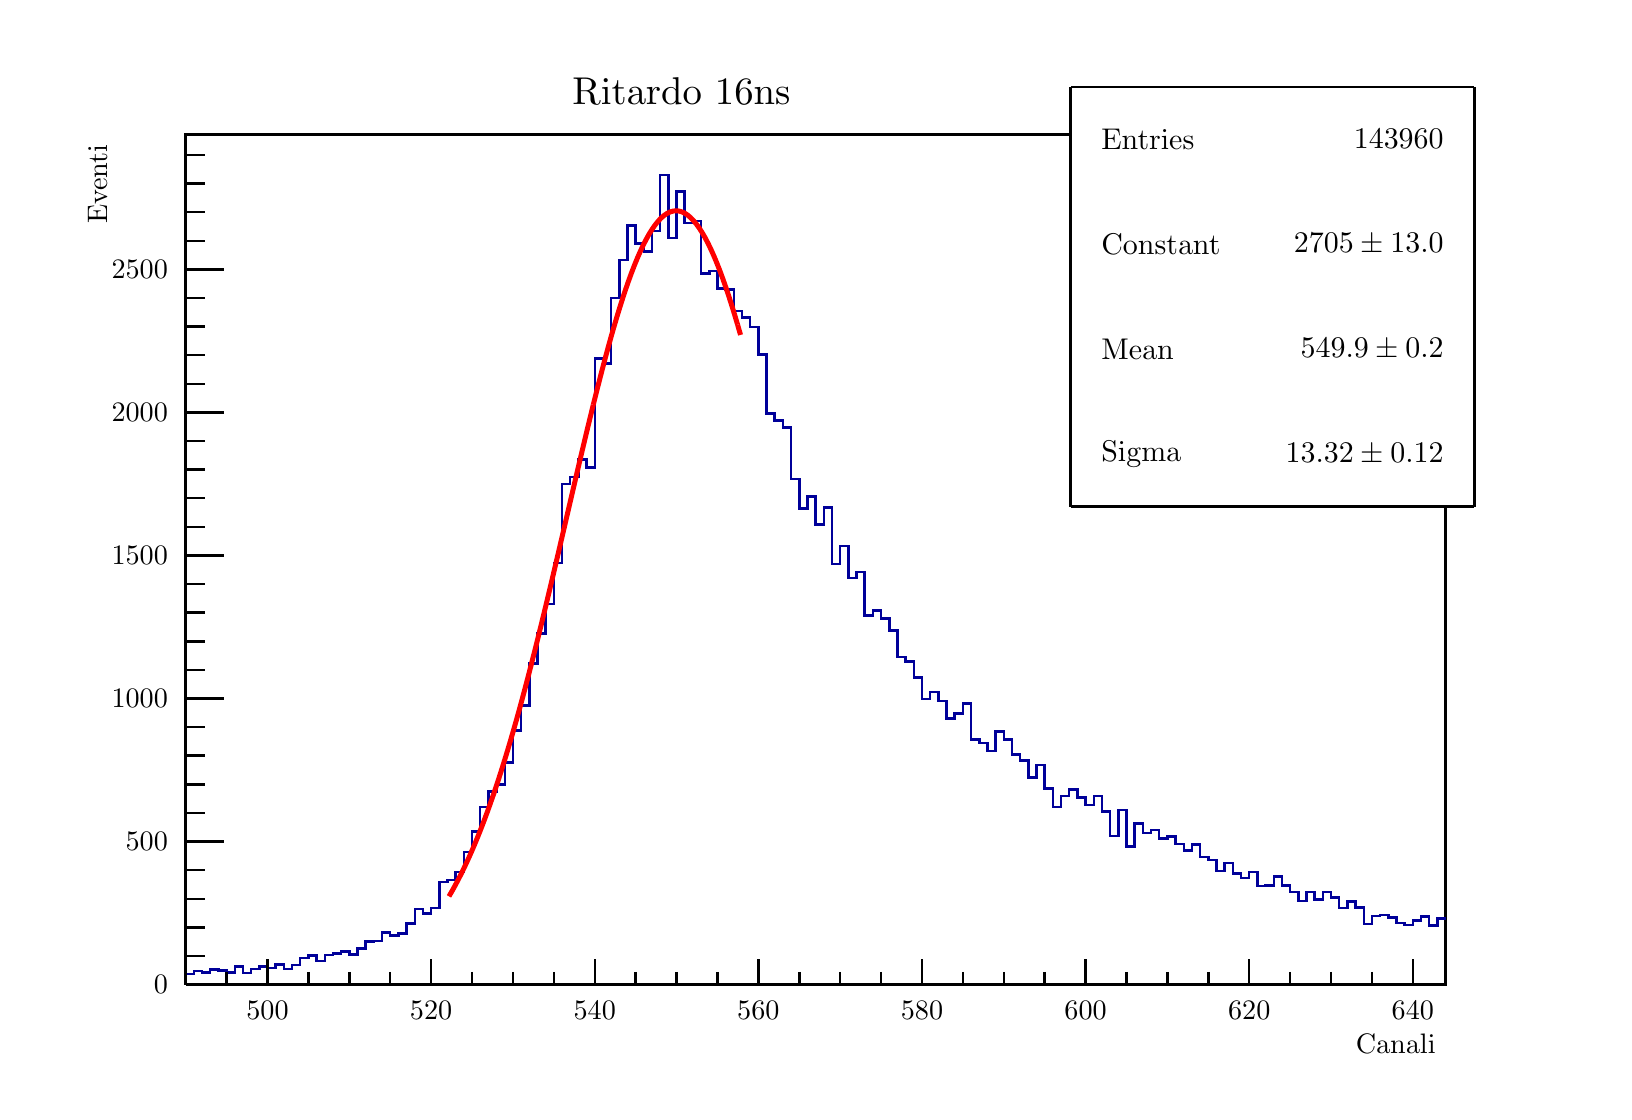
\begin{tikzpicture}
\pgfdeclareplotmark{cross} {
\pgfpathmoveto{\pgfpoint{-0.3\pgfplotmarksize}{\pgfplotmarksize}}
\pgfpathlineto{\pgfpoint{+0.3\pgfplotmarksize}{\pgfplotmarksize}}
\pgfpathlineto{\pgfpoint{+0.3\pgfplotmarksize}{0.3\pgfplotmarksize}}
\pgfpathlineto{\pgfpoint{+1\pgfplotmarksize}{0.3\pgfplotmarksize}}
\pgfpathlineto{\pgfpoint{+1\pgfplotmarksize}{-0.3\pgfplotmarksize}}
\pgfpathlineto{\pgfpoint{+0.3\pgfplotmarksize}{-0.3\pgfplotmarksize}}
\pgfpathlineto{\pgfpoint{+0.3\pgfplotmarksize}{-1.\pgfplotmarksize}}
\pgfpathlineto{\pgfpoint{-0.3\pgfplotmarksize}{-1.\pgfplotmarksize}}
\pgfpathlineto{\pgfpoint{-0.3\pgfplotmarksize}{-0.3\pgfplotmarksize}}
\pgfpathlineto{\pgfpoint{-1.\pgfplotmarksize}{-0.3\pgfplotmarksize}}
\pgfpathlineto{\pgfpoint{-1.\pgfplotmarksize}{0.3\pgfplotmarksize}}
\pgfpathlineto{\pgfpoint{-0.3\pgfplotmarksize}{0.3\pgfplotmarksize}}
\pgfpathclose
\pgfusepathqstroke
}
\pgfdeclareplotmark{cross*} {
\pgfpathmoveto{\pgfpoint{-0.3\pgfplotmarksize}{\pgfplotmarksize}}
\pgfpathlineto{\pgfpoint{+0.3\pgfplotmarksize}{\pgfplotmarksize}}
\pgfpathlineto{\pgfpoint{+0.3\pgfplotmarksize}{0.3\pgfplotmarksize}}
\pgfpathlineto{\pgfpoint{+1\pgfplotmarksize}{0.3\pgfplotmarksize}}
\pgfpathlineto{\pgfpoint{+1\pgfplotmarksize}{-0.3\pgfplotmarksize}}
\pgfpathlineto{\pgfpoint{+0.3\pgfplotmarksize}{-0.3\pgfplotmarksize}}
\pgfpathlineto{\pgfpoint{+0.3\pgfplotmarksize}{-1.\pgfplotmarksize}}
\pgfpathlineto{\pgfpoint{-0.3\pgfplotmarksize}{-1.\pgfplotmarksize}}
\pgfpathlineto{\pgfpoint{-0.3\pgfplotmarksize}{-0.3\pgfplotmarksize}}
\pgfpathlineto{\pgfpoint{-1.\pgfplotmarksize}{-0.3\pgfplotmarksize}}
\pgfpathlineto{\pgfpoint{-1.\pgfplotmarksize}{0.3\pgfplotmarksize}}
\pgfpathlineto{\pgfpoint{-0.3\pgfplotmarksize}{0.3\pgfplotmarksize}}
\pgfpathclose
\pgfusepathqfillstroke
}
\pgfdeclareplotmark{newstar} {
\pgfpathmoveto{\pgfqpoint{0pt}{\pgfplotmarksize}}
\pgfpathlineto{\pgfqpointpolar{44}{0.5\pgfplotmarksize}}
\pgfpathlineto{\pgfqpointpolar{18}{\pgfplotmarksize}}
\pgfpathlineto{\pgfqpointpolar{-20}{0.5\pgfplotmarksize}}
\pgfpathlineto{\pgfqpointpolar{-54}{\pgfplotmarksize}}
\pgfpathlineto{\pgfqpointpolar{-90}{0.5\pgfplotmarksize}}
\pgfpathlineto{\pgfqpointpolar{234}{\pgfplotmarksize}}
\pgfpathlineto{\pgfqpointpolar{198}{0.5\pgfplotmarksize}}
\pgfpathlineto{\pgfqpointpolar{162}{\pgfplotmarksize}}
\pgfpathlineto{\pgfqpointpolar{134}{0.5\pgfplotmarksize}}
\pgfpathclose
\pgfusepathqstroke
}
\pgfdeclareplotmark{newstar*} {
\pgfpathmoveto{\pgfqpoint{0pt}{\pgfplotmarksize}}
\pgfpathlineto{\pgfqpointpolar{44}{0.5\pgfplotmarksize}}
\pgfpathlineto{\pgfqpointpolar{18}{\pgfplotmarksize}}
\pgfpathlineto{\pgfqpointpolar{-20}{0.5\pgfplotmarksize}}
\pgfpathlineto{\pgfqpointpolar{-54}{\pgfplotmarksize}}
\pgfpathlineto{\pgfqpointpolar{-90}{0.5\pgfplotmarksize}}
\pgfpathlineto{\pgfqpointpolar{234}{\pgfplotmarksize}}
\pgfpathlineto{\pgfqpointpolar{198}{0.5\pgfplotmarksize}}
\pgfpathlineto{\pgfqpointpolar{162}{\pgfplotmarksize}}
\pgfpathlineto{\pgfqpointpolar{134}{0.5\pgfplotmarksize}}
\pgfpathclose
\pgfusepathqfillstroke
}
\definecolor{c}{rgb}{1,1,1};
\draw [color=c, fill=c] (0,0) rectangle (20,13.4957);
\draw [color=c, fill=c] (2,1.34957) rectangle (18,12.1461);
\definecolor{c}{rgb}{0,0,0};
\draw [c,line width=0.9] (2,1.34957) -- (2,12.1461) -- (18,12.1461) -- (18,1.34957) -- (2,1.34957);
\definecolor{c}{rgb}{1,1,1};
\draw [color=c, fill=c] (2,1.34957) rectangle (18,12.1461);
\definecolor{c}{rgb}{0,0,0};
\draw [c,line width=0.9] (2,1.34957) -- (2,12.1461) -- (18,12.1461) -- (18,1.34957) -- (2,1.34957);
\definecolor{c}{rgb}{0,0,0.6};
\draw [c,line width=0.9] (2,1.48401) -- (2.1039,1.48401) -- (2.1039,1.52034) -- (2.20779,1.52034) -- (2.20779,1.50581) -- (2.31169,1.50581) -- (2.31169,1.53851) -- (2.41558,1.53851) -- (2.41558,1.53124) -- (2.51948,1.53124) -- (2.51948,1.50581) --
 (2.62338,1.50581) -- (2.62338,1.57847) -- (2.72727,1.57847) -- (2.72727,1.49854) -- (2.83117,1.49854) -- (2.83117,1.54577) -- (2.93507,1.54577) -- (2.93507,1.58211) -- (3.03896,1.58211) -- (3.03896,1.56031) -- (3.14286,1.56031) -- (3.14286,1.60754)
 -- (3.24675,1.60754) -- (3.24675,1.54577) -- (3.35065,1.54577) -- (3.35065,1.59664) -- (3.45455,1.59664) -- (3.45455,1.68747) -- (3.55844,1.68747) -- (3.55844,1.71654) -- (3.66234,1.71654) -- (3.66234,1.64751) -- (3.76623,1.64751) --
 (3.76623,1.72381) -- (3.87013,1.72381) -- (3.87013,1.74561) -- (3.97403,1.74561) -- (3.97403,1.76741) -- (4.07792,1.76741) -- (4.07792,1.73107) -- (4.18182,1.73107) -- (4.18182,1.80738) -- (4.28571,1.80738) -- (4.28571,1.89821) -- (4.38961,1.89821)
 -- (4.38961,1.90184) -- (4.49351,1.90184) -- (4.49351,2.01448) -- (4.5974,2.01448) -- (4.5974,1.97451) -- (4.7013,1.97451) -- (4.7013,1.99994) -- (4.80519,1.99994) -- (4.80519,2.12711) -- (4.90909,2.12711) -- (4.90909,2.30878) -- (5.01299,2.30878)
 -- (5.01299,2.25065) -- (5.11688,2.25065) -- (5.11688,2.32331) -- (5.22078,2.32331) -- (5.22078,2.65032) -- (5.32468,2.65032) -- (5.32468,2.67938) -- (5.42857,2.67938) -- (5.42857,2.77749) -- (5.53247,2.77749) -- (5.53247,3.03182) --
 (5.63636,3.03182) -- (5.63636,3.29342) -- (5.74026,3.29342) -- (5.74026,3.60589) -- (5.84416,3.60589) -- (5.84416,3.8021) -- (5.94805,3.8021) -- (5.94805,3.8893) -- (6.05195,3.8893) -- (6.05195,4.1727) -- (6.15584,4.1727) -- (6.15584,4.576) --
 (6.25974,4.576) -- (6.25974,4.89574) -- (6.36364,4.89574) -- (6.36364,5.42621) -- (6.46753,5.42621) -- (6.46753,5.80772) -- (6.57143,5.80772) -- (6.57143,6.18559) -- (6.67532,6.18559) -- (6.67532,6.70516) -- (6.77922,6.70516) -- (6.77922,7.70797) --
 (6.88312,7.70797) -- (6.88312,7.79517) -- (6.98701,7.79517) -- (6.98701,8.02044) -- (7.09091,8.02044) -- (7.09091,7.9187) -- (7.19481,7.9187) -- (7.19481,9.29939) -- (7.2987,9.29939) -- (7.2987,9.23762) -- (7.4026,9.23762) -- (7.4026,10.0697) --
 (7.50649,10.0697) -- (7.50649,10.5493) -- (7.61039,10.5493) -- (7.61039,10.9925) -- (7.71429,10.9925) -- (7.71429,10.7636) -- (7.81818,10.7636) -- (7.81818,10.6619) -- (7.92208,10.6619) -- (7.92208,10.9199) -- (8.02597,10.9199) -- (8.02597,11.632)
 -- (8.12987,11.632) -- (8.12987,10.829) -- (8.23377,10.829) -- (8.23377,11.4249) -- (8.33766,11.4249) -- (8.33766,11.0216) -- (8.44156,11.0216) -- (8.44156,11.047) -- (8.54545,11.047) -- (8.54545,10.3785) -- (8.64935,10.3785) -- (8.64935,10.4148) --
 (8.75325,10.4148) -- (8.75325,10.1896) -- (8.85714,10.1896) -- (8.85714,10.175) -- (8.96104,10.175) -- (8.96104,9.90616) -- (9.06493,9.90616) -- (9.06493,9.82259) -- (9.16883,9.82259) -- (9.16883,9.70269) -- (9.27273,9.70269) -- (9.27273,9.35025) --
 (9.37662,9.35025) -- (9.37662,8.60541) -- (9.48052,8.60541) -- (9.48052,8.51458) -- (9.58442,8.51458) -- (9.58442,8.42374) -- (9.68831,8.42374) -- (9.68831,7.77337) -- (9.79221,7.77337) -- (9.79221,7.3955) -- (9.8961,7.3955) -- (9.8961,7.5481) --
 (10,7.5481) -- (10,7.19566) -- (10.1039,7.19566) -- (10.1039,7.4064) -- (10.2078,7.4064) -- (10.2078,6.69426) -- (10.3117,6.69426) -- (10.3117,6.91953) -- (10.4156,6.91953) -- (10.4156,6.51622) -- (10.5195,6.51622) -- (10.5195,6.59252) --
 (10.6234,6.59252) -- (10.6234,6.03662) -- (10.7273,6.03662) -- (10.7273,6.09839) -- (10.8312,6.09839) -- (10.8312,6.00028) -- (10.9351,6.00028) -- (10.9351,5.84405) -- (11.039,5.84405) -- (11.039,5.50978) -- (11.1429,5.50978) -- (11.1429,5.45528) --
 (11.2468,5.45528) -- (11.2468,5.24818) -- (11.3506,5.24818) -- (11.3506,4.97931) -- (11.4545,4.97931) -- (11.4545,5.06288) -- (11.5584,5.06288) -- (11.5584,4.95387) -- (11.6623,4.95387) -- (11.6623,4.73224) -- (11.7662,4.73224) -- (11.7662,4.79037)
 -- (11.8701,4.79037) -- (11.8701,4.91754) -- (11.974,4.91754) -- (11.974,4.45974) -- (12.0779,4.45974) -- (12.0779,4.41614) -- (12.1818,4.41614) -- (12.1818,4.31803) -- (12.2857,4.31803) -- (12.2857,4.56147) -- (12.3896,4.56147) -- (12.3896,4.45974)
 -- (12.4935,4.45974) -- (12.4935,4.2708) -- (12.5974,4.2708) -- (12.5974,4.1945) -- (12.7013,4.1945) -- (12.7013,3.98013) -- (12.8052,3.98013) -- (12.8052,4.13637) -- (12.9091,4.13637) -- (12.9091,3.83843) -- (13.013,3.83843) -- (13.013,3.60226) --
 (13.1169,3.60226) -- (13.1169,3.7476) -- (13.2208,3.7476) -- (13.2208,3.82753) -- (13.3247,3.82753) -- (13.3247,3.72579) -- (13.4286,3.72579) -- (13.4286,3.62769) -- (13.5325,3.62769) -- (13.5325,3.74396) -- (13.6364,3.74396) -- (13.6364,3.54776) --
 (13.7403,3.54776) -- (13.7403,3.23529) -- (13.8442,3.23529) -- (13.8442,3.56593) -- (13.9481,3.56593) -- (13.9481,3.10449) -- (14.0519,3.10449) -- (14.0519,3.39516) -- (14.1558,3.39516) -- (14.1558,3.27526) -- (14.2597,3.27526) -- (14.2597,3.31159)
 -- (14.3636,3.31159) -- (14.3636,3.20259) -- (14.4675,3.20259) -- (14.4675,3.23166) -- (14.5714,3.23166) -- (14.5714,3.13719) -- (14.6753,3.13719) -- (14.6753,3.05362) -- (14.7792,3.05362) -- (14.7792,3.12629) -- (14.8831,3.12629) --
 (14.8831,2.97005) -- (14.987,2.97005) -- (14.987,2.93009) -- (15.0909,2.93009) -- (15.0909,2.79565) -- (15.1948,2.79565) -- (15.1948,2.89375) -- (15.2987,2.89375) -- (15.2987,2.76295) -- (15.4026,2.76295) -- (15.4026,2.70118) -- (15.5065,2.70118) --
 (15.5065,2.77749) -- (15.6104,2.77749) -- (15.6104,2.59945) -- (15.7143,2.59945) -- (15.7143,2.60672) -- (15.8182,2.60672) -- (15.8182,2.72298) -- (15.9221,2.72298) -- (15.9221,2.61035) -- (16.026,2.61035) -- (16.026,2.52315) -- (16.1299,2.52315) --
 (16.1299,2.41051) -- (16.2338,2.41051) -- (16.2338,2.52315) -- (16.3377,2.52315) -- (16.3377,2.43231) -- (16.4416,2.43231) -- (16.4416,2.52315) -- (16.5455,2.52315) -- (16.5455,2.45412) -- (16.6494,2.45412) -- (16.6494,2.31968) -- (16.7532,2.31968)
 -- (16.7532,2.40325) -- (16.8571,2.40325) -- (16.8571,2.33058) -- (16.961,2.33058) -- (16.961,2.11621) -- (17.0649,2.11621) -- (17.0649,2.22158) -- (17.1688,2.22158) -- (17.1688,2.23611) -- (17.2727,2.23611) -- (17.2727,2.19978) -- (17.3766,2.19978)
 -- (17.3766,2.13438) -- (17.4805,2.13438) -- (17.4805,2.10531) -- (17.5844,2.10531) -- (17.5844,2.16345) -- (17.6883,2.16345) -- (17.6883,2.21431) -- (17.7922,2.21431) -- (17.7922,2.09804) -- (17.8961,2.09804) -- (17.8961,2.18888) -- (18,2.18888);
\definecolor{c}{rgb}{1,1,1};
\draw [color=c, fill=c] (13.2378,7.4212) rectangle (18.3668,12.7507);
\definecolor{c}{rgb}{0,0,0};
\draw [c,line width=0.9] (13.2378,7.4212) -- (18.3668,7.4212);
\draw [c,line width=0.9] (18.3668,7.4212) -- (18.3668,12.7507);
\draw [c,line width=0.9] (18.3668,12.7507) -- (13.2378,12.7507);
\draw [c,line width=0.9] (13.2378,12.7507) -- (13.2378,7.4212);
\draw [anchor= west] (13.4943,12.0845) node[scale=1.08185, color=c, rotate=0]{Entries };
\draw [anchor= east] (18.1103,12.0845) node[scale=1.08185, color=c, rotate=0]{ 143960};
\draw [anchor= west] (13.4943,10.7521) node[scale=1.08185, color=c, rotate=0]{Constant };
\draw [anchor= east] (18.1103,10.7521) node[scale=1.08185, color=c, rotate=0]{$  2705 \pm 13.0$};
\draw [anchor= west] (13.4943,9.41977) node[scale=1.08185, color=c, rotate=0]{Mean     };
\draw [anchor= east] (18.1103,9.41977) node[scale=1.08185, color=c, rotate=0]{$ 549.9 \pm 0.2$};
\draw [anchor= west] (13.4943,8.08739) node[scale=1.08185, color=c, rotate=0]{Sigma    };
\draw [anchor= east] (18.1103,8.08739) node[scale=1.08185, color=c, rotate=0]{$ 13.32 \pm 0.12$};
\definecolor{c}{rgb}{1,0,0};
\draw [c,line width=1.8] (5.34338,2.47036) -- (5.38078,2.53485) -- (5.41818,2.60213) -- (5.45558,2.67227) -- (5.49299,2.74532) -- (5.53039,2.82132) -- (5.56779,2.90033) -- (5.6052,2.98239) -- (5.6426,3.06754) -- (5.68,3.15581) -- (5.7174,3.24723) --
 (5.75481,3.34182) -- (5.79221,3.43959) -- (5.82961,3.54057) -- (5.86701,3.64475) -- (5.90442,3.75212) -- (5.94182,3.86268) -- (5.97922,3.97642) -- (6.01662,4.09329) -- (6.05403,4.21327) -- (6.09143,4.33632) -- (6.12883,4.46239) -- (6.16623,4.5914)
 -- (6.20364,4.7233) -- (6.24104,4.858) -- (6.27844,4.99541) -- (6.31584,5.13545) -- (6.35325,5.27799) -- (6.39065,5.42292) -- (6.42805,5.57012) -- (6.46545,5.71944) -- (6.50286,5.87074) -- (6.54026,6.02387) -- (6.57766,6.17866) -- (6.61507,6.33493)
 -- (6.65247,6.4925) -- (6.68987,6.65118) -- (6.72727,6.81077) -- (6.76468,6.97105) -- (6.80208,7.13182) -- (6.83948,7.29284) -- (6.87688,7.45388) -- (6.91429,7.61472) -- (6.95169,7.77509) -- (6.98909,7.93476) -- (7.02649,8.09348) -- (7.0639,8.25097)
 -- (7.1013,8.40699) -- (7.1387,8.56127) -- (7.1761,8.71354);
\draw [c,line width=1.8] (7.1761,8.71354) -- (7.21351,8.86354) -- (7.25091,9.011) -- (7.28831,9.15565) -- (7.32571,9.29723) -- (7.36312,9.43546) -- (7.40052,9.5701) -- (7.43792,9.70088) -- (7.47532,9.82754) -- (7.51273,9.94984) -- (7.55013,10.0675)
 -- (7.58753,10.1804) -- (7.62494,10.2882) -- (7.66234,10.3907) -- (7.69974,10.4877) -- (7.73714,10.579) -- (7.77455,10.6644) -- (7.81195,10.7437) -- (7.84935,10.8168) -- (7.88675,10.8836) -- (7.92416,10.9437) -- (7.96156,10.9972) --
 (7.99896,11.0439) -- (8.03636,11.0838) -- (8.07377,11.1166) -- (8.11117,11.1424) -- (8.14857,11.1611) -- (8.18597,11.1727) -- (8.22338,11.1771) -- (8.26078,11.1744) -- (8.29818,11.1644) -- (8.33558,11.1474) -- (8.37299,11.1232) -- (8.41039,11.0919)
 -- (8.44779,11.0537) -- (8.4852,11.0086) -- (8.5226,10.9566) -- (8.56,10.898) -- (8.5974,10.8328) -- (8.63481,10.7611) -- (8.67221,10.6832) -- (8.70961,10.5992) -- (8.74701,10.5092) -- (8.78442,10.4135) -- (8.82182,10.3122) -- (8.85922,10.2056) --
 (8.89662,10.0939) -- (8.93403,9.97733) -- (8.97143,9.85606) -- (9.00883,9.73038);
\draw [c,line width=1.8] (9.00883,9.73038) -- (9.04623,9.60052);
\definecolor{c}{rgb}{0,0,0};
\draw [c,line width=0.9] (2,1.34957) -- (18,1.34957);
\draw [anchor= east] (18,0.593811) node[scale=1.01821, color=c, rotate=0]{Canali};
\draw [c,line width=0.9] (3.03896,1.67347) -- (3.03896,1.34957);
\draw [c,line width=0.9] (3.55844,1.51152) -- (3.55844,1.34957);
\draw [c,line width=0.9] (4.07792,1.51152) -- (4.07792,1.34957);
\draw [c,line width=0.9] (4.5974,1.51152) -- (4.5974,1.34957);
\draw [c,line width=0.9] (5.11688,1.67347) -- (5.11688,1.34957);
\draw [c,line width=0.9] (5.63636,1.51152) -- (5.63636,1.34957);
\draw [c,line width=0.9] (6.15584,1.51152) -- (6.15584,1.34957);
\draw [c,line width=0.9] (6.67532,1.51152) -- (6.67532,1.34957);
\draw [c,line width=0.9] (7.19481,1.67347) -- (7.19481,1.34957);
\draw [c,line width=0.9] (7.71429,1.51152) -- (7.71429,1.34957);
\draw [c,line width=0.9] (8.23377,1.51152) -- (8.23377,1.34957);
\draw [c,line width=0.9] (8.75325,1.51152) -- (8.75325,1.34957);
\draw [c,line width=0.9] (9.27273,1.67347) -- (9.27273,1.34957);
\draw [c,line width=0.9] (9.79221,1.51152) -- (9.79221,1.34957);
\draw [c,line width=0.9] (10.3117,1.51152) -- (10.3117,1.34957);
\draw [c,line width=0.9] (10.8312,1.51152) -- (10.8312,1.34957);
\draw [c,line width=0.9] (11.3506,1.67347) -- (11.3506,1.34957);
\draw [c,line width=0.9] (11.8701,1.51152) -- (11.8701,1.34957);
\draw [c,line width=0.9] (12.3896,1.51152) -- (12.3896,1.34957);
\draw [c,line width=0.9] (12.9091,1.51152) -- (12.9091,1.34957);
\draw [c,line width=0.9] (13.4286,1.67347) -- (13.4286,1.34957);
\draw [c,line width=0.9] (13.9481,1.51152) -- (13.9481,1.34957);
\draw [c,line width=0.9] (14.4675,1.51152) -- (14.4675,1.34957);
\draw [c,line width=0.9] (14.987,1.51152) -- (14.987,1.34957);
\draw [c,line width=0.9] (15.5065,1.67347) -- (15.5065,1.34957);
\draw [c,line width=0.9] (16.026,1.51152) -- (16.026,1.34957);
\draw [c,line width=0.9] (16.5455,1.51152) -- (16.5455,1.34957);
\draw [c,line width=0.9] (17.0649,1.51152) -- (17.0649,1.34957);
\draw [c,line width=0.9] (17.5844,1.67347) -- (17.5844,1.34957);
\draw [c,line width=0.9] (3.03896,1.67347) -- (3.03896,1.34957);
\draw [c,line width=0.9] (2.51948,1.51152) -- (2.51948,1.34957);
\draw [c,line width=0.9] (2,1.51152) -- (2,1.34957);
\draw [c,line width=0.9] (17.5844,1.67347) -- (17.5844,1.34957);
\draw [anchor=base] (3.03896,0.904212) node[scale=1.01821, color=c, rotate=0]{500};
\draw [anchor=base] (5.11688,0.904212) node[scale=1.01821, color=c, rotate=0]{520};
\draw [anchor=base] (7.19481,0.904212) node[scale=1.01821, color=c, rotate=0]{540};
\draw [anchor=base] (9.27273,0.904212) node[scale=1.01821, color=c, rotate=0]{560};
\draw [anchor=base] (11.3506,0.904212) node[scale=1.01821, color=c, rotate=0]{580};
\draw [anchor=base] (13.4286,0.904212) node[scale=1.01821, color=c, rotate=0]{600};
\draw [anchor=base] (15.5065,0.904212) node[scale=1.01821, color=c, rotate=0]{620};
\draw [anchor=base] (17.5844,0.904212) node[scale=1.01821, color=c, rotate=0]{640};
\draw [c,line width=0.9] (2,1.34957) -- (2,12.1461);
\draw [anchor= east] (0.88,12.1461) node[scale=1.01821, color=c, rotate=90]{Eventi};
\draw [c,line width=0.9] (2.48,1.34957) -- (2,1.34957);
\draw [c,line width=0.9] (2.24,1.71291) -- (2,1.71291);
\draw [c,line width=0.9] (2.24,2.07624) -- (2,2.07624);
\draw [c,line width=0.9] (2.24,2.43958) -- (2,2.43958);
\draw [c,line width=0.9] (2.24,2.80292) -- (2,2.80292);
\draw [c,line width=0.9] (2.48,3.16626) -- (2,3.16626);
\draw [c,line width=0.9] (2.24,3.52959) -- (2,3.52959);
\draw [c,line width=0.9] (2.24,3.89293) -- (2,3.89293);
\draw [c,line width=0.9] (2.24,4.25627) -- (2,4.25627);
\draw [c,line width=0.9] (2.24,4.6196) -- (2,4.6196);
\draw [c,line width=0.9] (2.48,4.98294) -- (2,4.98294);
\draw [c,line width=0.9] (2.24,5.34628) -- (2,5.34628);
\draw [c,line width=0.9] (2.24,5.70962) -- (2,5.70962);
\draw [c,line width=0.9] (2.24,6.07295) -- (2,6.07295);
\draw [c,line width=0.9] (2.24,6.43629) -- (2,6.43629);
\draw [c,line width=0.9] (2.48,6.79963) -- (2,6.79963);
\draw [c,line width=0.9] (2.24,7.16296) -- (2,7.16296);
\draw [c,line width=0.9] (2.24,7.5263) -- (2,7.5263);
\draw [c,line width=0.9] (2.24,7.88964) -- (2,7.88964);
\draw [c,line width=0.9] (2.24,8.25297) -- (2,8.25297);
\draw [c,line width=0.9] (2.48,8.61631) -- (2,8.61631);
\draw [c,line width=0.9] (2.24,8.97965) -- (2,8.97965);
\draw [c,line width=0.9] (2.24,9.34299) -- (2,9.34299);
\draw [c,line width=0.9] (2.24,9.70632) -- (2,9.70632);
\draw [c,line width=0.9] (2.24,10.0697) -- (2,10.0697);
\draw [c,line width=0.9] (2.48,10.433) -- (2,10.433);
\draw [c,line width=0.9] (2.48,10.433) -- (2,10.433);
\draw [c,line width=0.9] (2.24,10.7963) -- (2,10.7963);
\draw [c,line width=0.9] (2.24,11.1597) -- (2,11.1597);
\draw [c,line width=0.9] (2.24,11.523) -- (2,11.523);
\draw [c,line width=0.9] (2.24,11.8863) -- (2,11.8863);
\draw [anchor= east] (1.9,1.34957) node[scale=1.01821, color=c, rotate=0]{0};
\draw [anchor= east] (1.9,3.16626) node[scale=1.01821, color=c, rotate=0]{500};
\draw [anchor= east] (1.9,4.98294) node[scale=1.01821, color=c, rotate=0]{1000};
\draw [anchor= east] (1.9,6.79963) node[scale=1.01821, color=c, rotate=0]{1500};
\draw [anchor= east] (1.9,8.61631) node[scale=1.01821, color=c, rotate=0]{2000};
\draw [anchor= east] (1.9,10.433) node[scale=1.01821, color=c, rotate=0]{2500};
\definecolor{c}{rgb}{1,1,1};
\draw [color=c, fill=c] (13.2378,7.4212) rectangle (18.3668,12.7507);
\definecolor{c}{rgb}{0,0,0};
\draw [c,line width=0.9] (13.2378,7.4212) -- (18.3668,7.4212);
\draw [c,line width=0.9] (18.3668,7.4212) -- (18.3668,12.7507);
\draw [c,line width=0.9] (18.3668,12.7507) -- (13.2378,12.7507);
\draw [c,line width=0.9] (13.2378,12.7507) -- (13.2378,7.4212);
\draw [anchor= west] (13.4943,12.0845) node[scale=1.08185, color=c, rotate=0]{Entries };
\draw [anchor= east] (18.1103,12.0845) node[scale=1.08185, color=c, rotate=0]{ 143960};
\draw [anchor= west] (13.4943,10.7521) node[scale=1.08185, color=c, rotate=0]{Constant };
\draw [anchor= east] (18.1103,10.7521) node[scale=1.08185, color=c, rotate=0]{$  2705 \pm 13.0$};
\draw [anchor= west] (13.4943,9.41977) node[scale=1.08185, color=c, rotate=0]{Mean     };
\draw [anchor= east] (18.1103,9.41977) node[scale=1.08185, color=c, rotate=0]{$ 549.9 \pm 0.2$};
\draw [anchor= west] (13.4943,8.08739) node[scale=1.08185, color=c, rotate=0]{Sigma    };
\draw [anchor= east] (18.1103,8.08739) node[scale=1.08185, color=c, rotate=0]{$ 13.32 \pm 0.12$};
\draw (8.29513,12.6934) node[scale=1.40004, color=c, rotate=0]{Ritardo 16ns};
\end{tikzpicture}

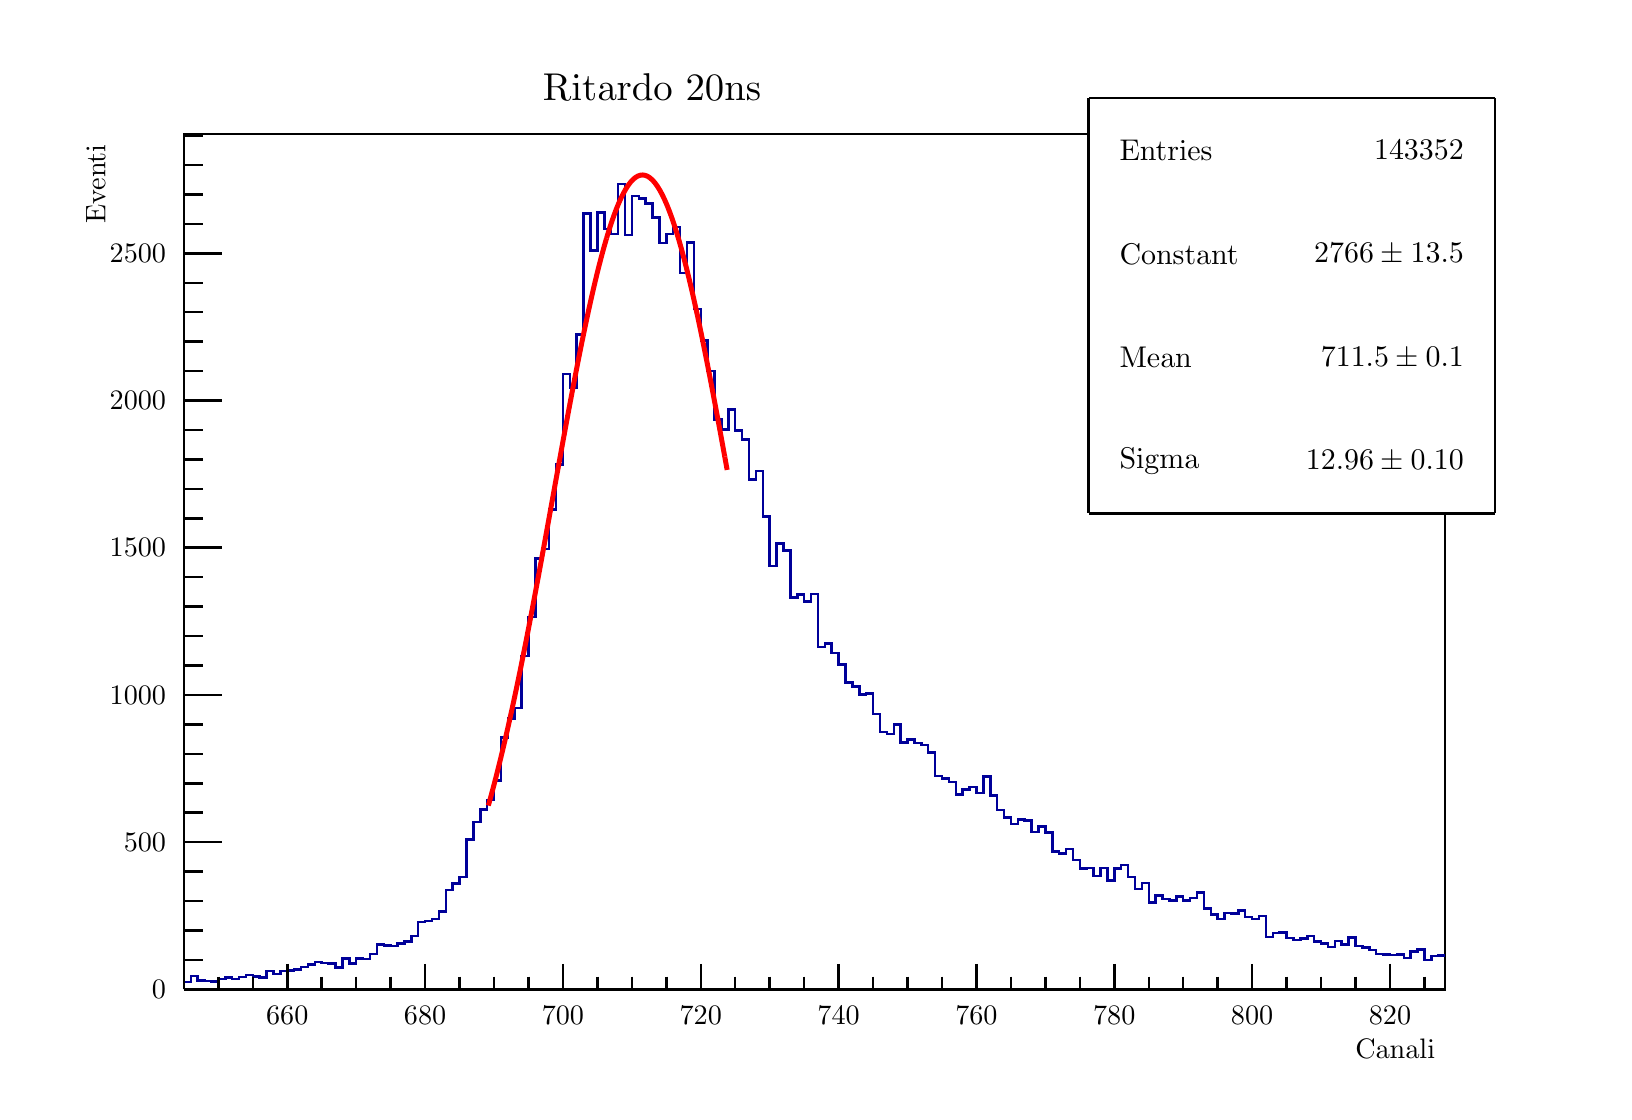
\begin{tikzpicture}
\pgfdeclareplotmark{cross} {
\pgfpathmoveto{\pgfpoint{-0.3\pgfplotmarksize}{\pgfplotmarksize}}
\pgfpathlineto{\pgfpoint{+0.3\pgfplotmarksize}{\pgfplotmarksize}}
\pgfpathlineto{\pgfpoint{+0.3\pgfplotmarksize}{0.3\pgfplotmarksize}}
\pgfpathlineto{\pgfpoint{+1\pgfplotmarksize}{0.3\pgfplotmarksize}}
\pgfpathlineto{\pgfpoint{+1\pgfplotmarksize}{-0.3\pgfplotmarksize}}
\pgfpathlineto{\pgfpoint{+0.3\pgfplotmarksize}{-0.3\pgfplotmarksize}}
\pgfpathlineto{\pgfpoint{+0.3\pgfplotmarksize}{-1.\pgfplotmarksize}}
\pgfpathlineto{\pgfpoint{-0.3\pgfplotmarksize}{-1.\pgfplotmarksize}}
\pgfpathlineto{\pgfpoint{-0.3\pgfplotmarksize}{-0.3\pgfplotmarksize}}
\pgfpathlineto{\pgfpoint{-1.\pgfplotmarksize}{-0.3\pgfplotmarksize}}
\pgfpathlineto{\pgfpoint{-1.\pgfplotmarksize}{0.3\pgfplotmarksize}}
\pgfpathlineto{\pgfpoint{-0.3\pgfplotmarksize}{0.3\pgfplotmarksize}}
\pgfpathclose
\pgfusepathqstroke
}
\pgfdeclareplotmark{cross*} {
\pgfpathmoveto{\pgfpoint{-0.3\pgfplotmarksize}{\pgfplotmarksize}}
\pgfpathlineto{\pgfpoint{+0.3\pgfplotmarksize}{\pgfplotmarksize}}
\pgfpathlineto{\pgfpoint{+0.3\pgfplotmarksize}{0.3\pgfplotmarksize}}
\pgfpathlineto{\pgfpoint{+1\pgfplotmarksize}{0.3\pgfplotmarksize}}
\pgfpathlineto{\pgfpoint{+1\pgfplotmarksize}{-0.3\pgfplotmarksize}}
\pgfpathlineto{\pgfpoint{+0.3\pgfplotmarksize}{-0.3\pgfplotmarksize}}
\pgfpathlineto{\pgfpoint{+0.3\pgfplotmarksize}{-1.\pgfplotmarksize}}
\pgfpathlineto{\pgfpoint{-0.3\pgfplotmarksize}{-1.\pgfplotmarksize}}
\pgfpathlineto{\pgfpoint{-0.3\pgfplotmarksize}{-0.3\pgfplotmarksize}}
\pgfpathlineto{\pgfpoint{-1.\pgfplotmarksize}{-0.3\pgfplotmarksize}}
\pgfpathlineto{\pgfpoint{-1.\pgfplotmarksize}{0.3\pgfplotmarksize}}
\pgfpathlineto{\pgfpoint{-0.3\pgfplotmarksize}{0.3\pgfplotmarksize}}
\pgfpathclose
\pgfusepathqfillstroke
}
\pgfdeclareplotmark{newstar} {
\pgfpathmoveto{\pgfqpoint{0pt}{\pgfplotmarksize}}
\pgfpathlineto{\pgfqpointpolar{44}{0.5\pgfplotmarksize}}
\pgfpathlineto{\pgfqpointpolar{18}{\pgfplotmarksize}}
\pgfpathlineto{\pgfqpointpolar{-20}{0.5\pgfplotmarksize}}
\pgfpathlineto{\pgfqpointpolar{-54}{\pgfplotmarksize}}
\pgfpathlineto{\pgfqpointpolar{-90}{0.5\pgfplotmarksize}}
\pgfpathlineto{\pgfqpointpolar{234}{\pgfplotmarksize}}
\pgfpathlineto{\pgfqpointpolar{198}{0.5\pgfplotmarksize}}
\pgfpathlineto{\pgfqpointpolar{162}{\pgfplotmarksize}}
\pgfpathlineto{\pgfqpointpolar{134}{0.5\pgfplotmarksize}}
\pgfpathclose
\pgfusepathqstroke
}
\pgfdeclareplotmark{newstar*} {
\pgfpathmoveto{\pgfqpoint{0pt}{\pgfplotmarksize}}
\pgfpathlineto{\pgfqpointpolar{44}{0.5\pgfplotmarksize}}
\pgfpathlineto{\pgfqpointpolar{18}{\pgfplotmarksize}}
\pgfpathlineto{\pgfqpointpolar{-20}{0.5\pgfplotmarksize}}
\pgfpathlineto{\pgfqpointpolar{-54}{\pgfplotmarksize}}
\pgfpathlineto{\pgfqpointpolar{-90}{0.5\pgfplotmarksize}}
\pgfpathlineto{\pgfqpointpolar{234}{\pgfplotmarksize}}
\pgfpathlineto{\pgfqpointpolar{198}{0.5\pgfplotmarksize}}
\pgfpathlineto{\pgfqpointpolar{162}{\pgfplotmarksize}}
\pgfpathlineto{\pgfqpointpolar{134}{0.5\pgfplotmarksize}}
\pgfpathclose
\pgfusepathqfillstroke
}
\definecolor{c}{rgb}{1,1,1};
\draw [color=c, fill=c] (0,0) rectangle (20,13.4957);
\draw [color=c, fill=c] (1.97708,1.2894) rectangle (17.9943,12.149);
\definecolor{c}{rgb}{0,0,0};
\draw [c,line width=0.9] (1.97708,1.2894) -- (1.97708,12.149) -- (17.9943,12.149) -- (17.9943,1.2894) -- (1.97708,1.2894);
\definecolor{c}{rgb}{1,1,1};
\draw [color=c, fill=c] (1.97708,1.2894) rectangle (17.9943,12.149);
\definecolor{c}{rgb}{0,0,0};
\draw [c,line width=0.9] (1.97708,1.2894) -- (1.97708,12.149) -- (17.9943,12.149) -- (17.9943,1.2894) -- (1.97708,1.2894);
\definecolor{c}{rgb}{0,0,0.6};
\draw [c,line width=0.9] (1.97708,1.38287) -- (2.0646,1.38287) -- (2.0646,1.45765) -- (2.15213,1.45765) -- (2.15213,1.40157) -- (2.23965,1.40157) -- (2.23965,1.39783) -- (2.32718,1.39783) -- (2.32718,1.38661) -- (2.41471,1.38661) -- (2.41471,1.424)
 -- (2.50223,1.424) -- (2.50223,1.44269) -- (2.58976,1.44269) -- (2.58976,1.424) -- (2.67728,1.424) -- (2.67728,1.44643) -- (2.76481,1.44643) -- (2.76481,1.46887) -- (2.85233,1.46887) -- (2.85233,1.45391) -- (2.93986,1.45391) -- (2.93986,1.44269) --
 (3.02739,1.44269) -- (3.02739,1.52121) -- (3.11491,1.52121) -- (3.11491,1.48382) -- (3.20244,1.48382) -- (3.20244,1.52495) -- (3.28996,1.52495) -- (3.28996,1.52869) -- (3.37749,1.52869) -- (3.37749,1.5399) -- (3.46501,1.5399) -- (3.46501,1.57355) --
 (3.55254,1.57355) -- (3.55254,1.6072) -- (3.64006,1.6072) -- (3.64006,1.63712) -- (3.72759,1.63712) -- (3.72759,1.6259) -- (3.81512,1.6259) -- (3.81512,1.61468) -- (3.90264,1.61468) -- (3.90264,1.56982) -- (3.99017,1.56982) -- (3.99017,1.68198) --
 (4.07769,1.68198) -- (4.07769,1.61842) -- (4.16522,1.61842) -- (4.16522,1.68198) -- (4.25274,1.68198) -- (4.25274,1.6745) -- (4.34027,1.6745) -- (4.34027,1.73807) -- (4.4278,1.73807) -- (4.4278,1.86145) -- (4.51532,1.86145) -- (4.51532,1.84649) --
 (4.60285,1.84649) -- (4.60285,1.84275) -- (4.69037,1.84275) -- (4.69037,1.87267) -- (4.7779,1.87267) -- (4.7779,1.89884) -- (4.86542,1.89884) -- (4.86542,1.96988) -- (4.95295,1.96988) -- (4.95295,2.1456) -- (5.04047,2.1456) -- (5.04047,2.16056) --
 (5.128,2.16056) -- (5.128,2.18299) -- (5.21553,2.18299) -- (5.21553,2.28021) -- (5.30305,2.28021) -- (5.30305,2.54941) -- (5.39058,2.54941) -- (5.39058,2.6354) -- (5.4781,2.6354) -- (5.4781,2.71766) -- (5.56563,2.71766) -- (5.56563,3.1925) --
 (5.65315,3.1925) -- (5.65315,3.41683) -- (5.74068,3.41683) -- (5.74068,3.57386) -- (5.82821,3.57386) -- (5.82821,3.69351) -- (5.91573,3.69351) -- (5.91573,3.94027) -- (6.00326,3.94027) -- (6.00326,4.48989) -- (6.09078,4.48989) -- (6.09078,4.72918)
 -- (6.17831,4.72918) -- (6.17831,4.86004) -- (6.26583,4.86004) -- (6.26583,5.52556) -- (6.35336,5.52556) -- (6.35336,6.01536) -- (6.44089,6.01536) -- (6.44089,6.76314) -- (6.52841,6.76314) -- (6.52841,6.88278) -- (6.61594,6.88278) --
 (6.61594,7.38379) -- (6.70346,7.38379) -- (6.70346,7.95585) -- (6.79099,7.95585) -- (6.79099,9.10369) -- (6.87851,9.10369) -- (6.87851,8.9317) -- (6.96604,8.9317) -- (6.96604,9.6047) -- (7.05356,9.6047) -- (7.05356,11.1451) -- (7.14109,11.1451) --
 (7.14109,10.6703) -- (7.22862,10.6703) -- (7.22862,11.1526) -- (7.31614,11.1526) -- (7.31614,10.9432) -- (7.40367,10.9432) -- (7.40367,10.8834) -- (7.49119,10.8834) -- (7.49119,11.519) -- (7.57872,11.519) -- (7.57872,10.8684) -- (7.66624,10.8684) --
 (7.66624,11.3657) -- (7.75377,11.3657) -- (7.75377,11.3321) -- (7.8413,11.3321) -- (7.8413,11.2685) -- (7.92882,11.2685) -- (7.92882,11.0928) -- (8.01635,11.0928) -- (8.01635,10.7675) -- (8.10387,10.7675) -- (8.10387,10.8797) -- (8.1914,10.8797) --
 (8.1914,10.9694) -- (8.27892,10.9694) -- (8.27892,10.3861) -- (8.36645,10.3861) -- (8.36645,10.7712) -- (8.45397,10.7712) -- (8.45397,9.92998) -- (8.5415,9.92998) -- (8.5415,9.52992) -- (8.62903,9.52992) -- (8.62903,9.14481) -- (8.71655,9.14481) --
 (8.71655,8.5279) -- (8.80408,8.5279) -- (8.80408,8.40077) -- (8.8916,8.40077) -- (8.8916,8.65128) -- (8.97913,8.65128) -- (8.97913,8.38956) -- (9.06665,8.38956) -- (9.06665,8.26991) -- (9.15418,8.26991) -- (9.15418,7.76516) -- (9.24171,7.76516) --
 (9.24171,7.86985) -- (9.32923,7.86985) -- (9.32923,7.29406) -- (9.41676,7.29406) -- (9.41676,6.66593) -- (9.50428,6.66593) -- (9.50428,6.95008) -- (9.59181,6.95008) -- (9.59181,6.86409) -- (9.67933,6.86409) -- (9.67933,6.26587) -- (9.76686,6.26587)
 -- (9.76686,6.30325) -- (9.85438,6.30325) -- (9.85438,6.21726) -- (9.94191,6.21726) -- (9.94191,6.31073) -- (10.0294,6.31073) -- (10.0294,5.63399) -- (10.117,5.63399) -- (10.117,5.6826) -- (10.2045,5.6826) -- (10.2045,5.55922) -- (10.292,5.55922) --
 (10.292,5.4134) -- (10.3795,5.4134) -- (10.3795,5.18533) -- (10.4671,5.18533) -- (10.4671,5.13298) -- (10.5546,5.13298) -- (10.5546,5.03577) -- (10.6421,5.03577) -- (10.6421,5.04699) -- (10.7296,5.04699) -- (10.7296,4.78526) -- (10.8172,4.78526) --
 (10.8172,4.56093) -- (10.9047,4.56093) -- (10.9047,4.53476) -- (10.9922,4.53476) -- (10.9922,4.65066) -- (11.0797,4.65066) -- (11.0797,4.42259) -- (11.1673,4.42259) -- (11.1673,4.46372) -- (11.2548,4.46372) -- (11.2548,4.41511) -- (11.3423,4.41511)
 -- (11.3423,4.39268) -- (11.4298,4.39268) -- (11.4298,4.29921) -- (11.5174,4.29921) -- (11.5174,3.99636) -- (11.6049,3.99636) -- (11.6049,3.97019) -- (11.6924,3.97019) -- (11.6924,3.92532) -- (11.7799,3.92532) -- (11.7799,3.76455) --
 (11.8675,3.76455) -- (11.8675,3.82437) -- (11.955,3.82437) -- (11.955,3.85802) -- (12.0425,3.85802) -- (12.0425,3.78324) -- (12.1301,3.78324) -- (12.1301,3.99262) -- (12.2176,3.99262) -- (12.2176,3.75333) -- (12.3051,3.75333) -- (12.3051,3.56638) --
 (12.3926,3.56638) -- (12.3926,3.47291) -- (12.4802,3.47291) -- (12.4802,3.39066) -- (12.5677,3.39066) -- (12.5677,3.44674) -- (12.6552,3.44674) -- (12.6552,3.43552) -- (12.7427,3.43552) -- (12.7427,3.28597) -- (12.8303,3.28597) -- (12.8303,3.35701)
 -- (12.9178,3.35701) -- (12.9178,3.27849) -- (13.0053,3.27849) -- (13.0053,3.0392) -- (13.0928,3.0392) -- (13.0928,3.01677) -- (13.1804,3.01677) -- (13.1804,3.07285) -- (13.2679,3.07285) -- (13.2679,2.93451) -- (13.3554,2.93451) -- (13.3554,2.82608)
 -- (13.4429,2.82608) -- (13.4429,2.83356) -- (13.5305,2.83356) -- (13.5305,2.72887) -- (13.618,2.72887) -- (13.618,2.83356) -- (13.7055,2.83356) -- (13.7055,2.66905) -- (13.793,2.66905) -- (13.793,2.82234) -- (13.8806,2.82234) -- (13.8806,2.86721)
 -- (13.9681,2.86721) -- (13.9681,2.71392) -- (14.0556,2.71392) -- (14.0556,2.56436) -- (14.1431,2.56436) -- (14.1431,2.63914) -- (14.2307,2.63914) -- (14.2307,2.39237) -- (14.3182,2.39237) -- (14.3182,2.47837) -- (14.4057,2.47837) --
 (14.4057,2.43724) -- (14.4932,2.43724) -- (14.4932,2.41481) -- (14.5808,2.41481) -- (14.5808,2.47089) -- (14.6683,2.47089) -- (14.6683,2.41854) -- (14.7558,2.41854) -- (14.7558,2.45219) -- (14.8433,2.45219) -- (14.8433,2.51949) -- (14.9309,2.51949)
 -- (14.9309,2.31759) -- (15.0184,2.31759) -- (15.0184,2.24282) -- (15.1059,2.24282) -- (15.1059,2.18299) -- (15.1934,2.18299) -- (15.1934,2.25777) -- (15.281,2.25777) -- (15.281,2.25403) -- (15.3685,2.25403) -- (15.3685,2.29142) -- (15.456,2.29142)
 -- (15.456,2.20917) -- (15.5436,2.20917) -- (15.5436,2.18299) -- (15.6311,2.18299) -- (15.6311,2.22038) -- (15.7186,2.22038) -- (15.7186,1.95118) -- (15.8061,1.95118) -- (15.8061,2.00727) -- (15.8937,2.00727) -- (15.8937,2.011) -- (15.9812,2.011) --
 (15.9812,1.93997) -- (16.0687,1.93997) -- (16.0687,1.91753) -- (16.1562,1.91753) -- (16.1562,1.93623) -- (16.2438,1.93623) -- (16.2438,1.96614) -- (16.3313,1.96614) -- (16.3313,1.89884) -- (16.4188,1.89884) -- (16.4188,1.87267) -- (16.5063,1.87267)
 -- (16.5063,1.8278) -- (16.5939,1.8278) -- (16.5939,1.90258) -- (16.6814,1.90258) -- (16.6814,1.86145) -- (16.7689,1.86145) -- (16.7689,1.94744) -- (16.8564,1.94744) -- (16.8564,1.84275) -- (16.944,1.84275) -- (16.944,1.82032) -- (17.0315,1.82032)
 -- (17.0315,1.78667) -- (17.119,1.78667) -- (17.119,1.73807) -- (17.2065,1.73807) -- (17.2065,1.73059) -- (17.2941,1.73059) -- (17.2941,1.72311) -- (17.3816,1.72311) -- (17.3816,1.73433) -- (17.4691,1.73433) -- (17.4691,1.68572) -- (17.5566,1.68572)
 -- (17.5566,1.77172) -- (17.6442,1.77172) -- (17.6442,1.79789) -- (17.7317,1.79789) -- (17.7317,1.66329) -- (17.8192,1.66329) -- (17.8192,1.71563) -- (17.9067,1.71563) -- (17.9067,1.71937) -- (17.9943,1.71937);
\definecolor{c}{rgb}{1,1,1};
\draw [color=c, fill=c] (13.467,7.33524) rectangle (18.6246,12.6074);
\definecolor{c}{rgb}{0,0,0};
\draw [c,line width=0.9] (13.467,7.33524) -- (18.6246,7.33524);
\draw [c,line width=0.9] (18.6246,7.33524) -- (18.6246,12.6074);
\draw [c,line width=0.9] (18.6246,12.6074) -- (13.467,12.6074);
\draw [c,line width=0.9] (13.467,12.6074) -- (13.467,7.33524);
\draw [anchor= west] (13.7249,11.9484) node[scale=1.08185, color=c, rotate=0]{Entries };
\draw [anchor= east] (18.3668,11.9484) node[scale=1.08185, color=c, rotate=0]{ 143352};
\draw [anchor= west] (13.7249,10.6304) node[scale=1.08185, color=c, rotate=0]{Constant };
\draw [anchor= east] (18.3668,10.6304) node[scale=1.08185, color=c, rotate=0]{$  2766 \pm 13.5$};
\draw [anchor= west] (13.7249,9.31232) node[scale=1.08185, color=c, rotate=0]{Mean     };
\draw [anchor= east] (18.3668,9.31232) node[scale=1.08185, color=c, rotate=0]{$ 711.5 \pm 0.1$};
\draw [anchor= west] (13.7249,7.99427) node[scale=1.08185, color=c, rotate=0]{Sigma    };
\draw [anchor= east] (18.3668,7.99427) node[scale=1.08185, color=c, rotate=0]{$ 12.96 \pm 0.10$};
\definecolor{c}{rgb}{1,0,0};
\draw [c,line width=1.8] (5.84352,3.62333) -- (5.87416,3.73378) -- (5.90479,3.8476) -- (5.93542,3.96476) -- (5.96606,4.08525) -- (5.99669,4.20903) -- (6.02733,4.33607) -- (6.05796,4.46632) -- (6.08859,4.59972) -- (6.11923,4.73621) --
 (6.14986,4.87571) -- (6.1805,5.01813) -- (6.21113,5.16338) -- (6.24176,5.31136) -- (6.2724,5.46194) -- (6.30303,5.61501) -- (6.33367,5.77042) -- (6.3643,5.92803) -- (6.39493,6.08768) -- (6.42557,6.2492) -- (6.4562,6.41243) -- (6.48684,6.57716) --
 (6.51747,6.74322) -- (6.5481,6.91039) -- (6.57874,7.07845) -- (6.60937,7.2472) -- (6.64001,7.41639) -- (6.67064,7.58579) -- (6.70127,7.75516) -- (6.73191,7.92424) -- (6.76254,8.09278) -- (6.79318,8.26051) -- (6.82381,8.42717) -- (6.85444,8.59248) --
 (6.88508,8.75618) -- (6.91571,8.91797) -- (6.94635,9.07759) -- (6.97698,9.23475) -- (7.00761,9.38917) -- (7.03825,9.54057) -- (7.06888,9.68867) -- (7.09952,9.83319) -- (7.13015,9.97387) -- (7.16078,10.1104) -- (7.19142,10.2426) -- (7.22205,10.3701)
 -- (7.25269,10.4927) -- (7.28332,10.6102) -- (7.31395,10.7223) -- (7.34459,10.8288);
\draw [c,line width=1.8] (7.34459,10.8288) -- (7.37522,10.9294) -- (7.40586,11.024) -- (7.43649,11.1124) -- (7.46712,11.1943) -- (7.49776,11.2696) -- (7.52839,11.3382) -- (7.55902,11.3999) -- (7.58966,11.4545) -- (7.62029,11.502) -- (7.65093,11.5422)
 -- (7.68156,11.5751) -- (7.71219,11.6005) -- (7.74283,11.6185) -- (7.77346,11.6289) -- (7.8041,11.6319) -- (7.83473,11.6272) -- (7.86536,11.6151) -- (7.896,11.5954) -- (7.92663,11.5683) -- (7.95727,11.5338) -- (7.9879,11.4919) -- (8.01853,11.4428)
 -- (8.04917,11.3866) -- (8.0798,11.3233) -- (8.11044,11.2532) -- (8.14107,11.1764) -- (8.1717,11.093) -- (8.20234,11.0032) -- (8.23297,10.9072) -- (8.26361,10.8052) -- (8.29424,10.6975) -- (8.32487,10.5841) -- (8.35551,10.4655) -- (8.38614,10.3417)
 -- (8.41678,10.2131) -- (8.44741,10.0799) -- (8.47804,9.94244) -- (8.50868,9.80087) -- (8.53931,9.65552) -- (8.56995,9.50665) -- (8.60058,9.35454) -- (8.63121,9.19948) -- (8.66185,9.04174) -- (8.69248,8.8816) -- (8.72312,8.71935) --
 (8.75375,8.55527) -- (8.78438,8.38963) -- (8.81502,8.2227) -- (8.84565,8.05477);
\draw [c,line width=1.8] (8.84565,8.05477) -- (8.87629,7.88608);
\definecolor{c}{rgb}{0,0,0};
\draw [c,line width=0.9] (1.97708,1.2894) -- (17.9943,1.2894);
\draw [anchor= east] (17.9943,0.533639) node[scale=1.01821, color=c, rotate=0]{Canali};
\draw [c,line width=0.9] (3.28996,1.61364) -- (3.28996,1.2894);
\draw [c,line width=0.9] (3.72759,1.45152) -- (3.72759,1.2894);
\draw [c,line width=0.9] (4.16522,1.45152) -- (4.16522,1.2894);
\draw [c,line width=0.9] (4.60285,1.45152) -- (4.60285,1.2894);
\draw [c,line width=0.9] (5.04047,1.61364) -- (5.04047,1.2894);
\draw [c,line width=0.9] (5.4781,1.45152) -- (5.4781,1.2894);
\draw [c,line width=0.9] (5.91573,1.45152) -- (5.91573,1.2894);
\draw [c,line width=0.9] (6.35336,1.45152) -- (6.35336,1.2894);
\draw [c,line width=0.9] (6.79099,1.61364) -- (6.79099,1.2894);
\draw [c,line width=0.9] (7.22862,1.45152) -- (7.22862,1.2894);
\draw [c,line width=0.9] (7.66624,1.45152) -- (7.66624,1.2894);
\draw [c,line width=0.9] (8.10387,1.45152) -- (8.10387,1.2894);
\draw [c,line width=0.9] (8.5415,1.61364) -- (8.5415,1.2894);
\draw [c,line width=0.9] (8.97913,1.45152) -- (8.97913,1.2894);
\draw [c,line width=0.9] (9.41676,1.45152) -- (9.41676,1.2894);
\draw [c,line width=0.9] (9.85438,1.45152) -- (9.85438,1.2894);
\draw [c,line width=0.9] (10.292,1.61364) -- (10.292,1.2894);
\draw [c,line width=0.9] (10.7296,1.45152) -- (10.7296,1.2894);
\draw [c,line width=0.9] (11.1673,1.45152) -- (11.1673,1.2894);
\draw [c,line width=0.9] (11.6049,1.45152) -- (11.6049,1.2894);
\draw [c,line width=0.9] (12.0425,1.61364) -- (12.0425,1.2894);
\draw [c,line width=0.9] (12.4802,1.45152) -- (12.4802,1.2894);
\draw [c,line width=0.9] (12.9178,1.45152) -- (12.9178,1.2894);
\draw [c,line width=0.9] (13.3554,1.45152) -- (13.3554,1.2894);
\draw [c,line width=0.9] (13.793,1.61364) -- (13.793,1.2894);
\draw [c,line width=0.9] (14.2307,1.45152) -- (14.2307,1.2894);
\draw [c,line width=0.9] (14.6683,1.45152) -- (14.6683,1.2894);
\draw [c,line width=0.9] (15.1059,1.45152) -- (15.1059,1.2894);
\draw [c,line width=0.9] (15.5436,1.61364) -- (15.5436,1.2894);
\draw [c,line width=0.9] (15.9812,1.45152) -- (15.9812,1.2894);
\draw [c,line width=0.9] (16.4188,1.45152) -- (16.4188,1.2894);
\draw [c,line width=0.9] (16.8564,1.45152) -- (16.8564,1.2894);
\draw [c,line width=0.9] (17.2941,1.61364) -- (17.2941,1.2894);
\draw [c,line width=0.9] (3.28996,1.61364) -- (3.28996,1.2894);
\draw [c,line width=0.9] (2.85233,1.45152) -- (2.85233,1.2894);
\draw [c,line width=0.9] (2.41471,1.45152) -- (2.41471,1.2894);
\draw [c,line width=0.9] (17.2941,1.61364) -- (17.2941,1.2894);
\draw [c,line width=0.9] (17.7317,1.45152) -- (17.7317,1.2894);
\draw [anchor=base] (3.28996,0.84404) node[scale=1.01821, color=c, rotate=0]{660};
\draw [anchor=base] (5.04047,0.84404) node[scale=1.01821, color=c, rotate=0]{680};
\draw [anchor=base] (6.79099,0.84404) node[scale=1.01821, color=c, rotate=0]{700};
\draw [anchor=base] (8.5415,0.84404) node[scale=1.01821, color=c, rotate=0]{720};
\draw [anchor=base] (10.292,0.84404) node[scale=1.01821, color=c, rotate=0]{740};
\draw [anchor=base] (12.0425,0.84404) node[scale=1.01821, color=c, rotate=0]{760};
\draw [anchor=base] (13.793,0.84404) node[scale=1.01821, color=c, rotate=0]{780};
\draw [anchor=base] (15.5436,0.84404) node[scale=1.01821, color=c, rotate=0]{800};
\draw [anchor=base] (17.2941,0.84404) node[scale=1.01821, color=c, rotate=0]{820};
\draw [c,line width=0.9] (1.97708,1.2894) -- (1.97708,12.149);
\draw [anchor= east] (0.857077,12.149) node[scale=1.01821, color=c, rotate=90]{Eventi};
\draw [c,line width=0.9] (2.45988,1.2894) -- (1.97708,1.2894);
\draw [c,line width=0.9] (2.21848,1.66329) -- (1.97708,1.66329);
\draw [c,line width=0.9] (2.21848,2.03718) -- (1.97708,2.03718);
\draw [c,line width=0.9] (2.21848,2.41107) -- (1.97708,2.41107);
\draw [c,line width=0.9] (2.21848,2.78496) -- (1.97708,2.78496);
\draw [c,line width=0.9] (2.45988,3.15885) -- (1.97708,3.15885);
\draw [c,line width=0.9] (2.21848,3.53273) -- (1.97708,3.53273);
\draw [c,line width=0.9] (2.21848,3.90662) -- (1.97708,3.90662);
\draw [c,line width=0.9] (2.21848,4.28051) -- (1.97708,4.28051);
\draw [c,line width=0.9] (2.21848,4.6544) -- (1.97708,4.6544);
\draw [c,line width=0.9] (2.45988,5.02829) -- (1.97708,5.02829);
\draw [c,line width=0.9] (2.21848,5.40218) -- (1.97708,5.40218);
\draw [c,line width=0.9] (2.21848,5.77607) -- (1.97708,5.77607);
\draw [c,line width=0.9] (2.21848,6.14996) -- (1.97708,6.14996);
\draw [c,line width=0.9] (2.21848,6.52385) -- (1.97708,6.52385);
\draw [c,line width=0.9] (2.45988,6.89774) -- (1.97708,6.89774);
\draw [c,line width=0.9] (2.21848,7.27163) -- (1.97708,7.27163);
\draw [c,line width=0.9] (2.21848,7.64552) -- (1.97708,7.64552);
\draw [c,line width=0.9] (2.21848,8.01941) -- (1.97708,8.01941);
\draw [c,line width=0.9] (2.21848,8.3933) -- (1.97708,8.3933);
\draw [c,line width=0.9] (2.45988,8.76719) -- (1.97708,8.76719);
\draw [c,line width=0.9] (2.21848,9.14108) -- (1.97708,9.14108);
\draw [c,line width=0.9] (2.21848,9.51496) -- (1.97708,9.51496);
\draw [c,line width=0.9] (2.21848,9.88885) -- (1.97708,9.88885);
\draw [c,line width=0.9] (2.21848,10.2627) -- (1.97708,10.2627);
\draw [c,line width=0.9] (2.45988,10.6366) -- (1.97708,10.6366);
\draw [c,line width=0.9] (2.45988,10.6366) -- (1.97708,10.6366);
\draw [c,line width=0.9] (2.21848,11.0105) -- (1.97708,11.0105);
\draw [c,line width=0.9] (2.21848,11.3844) -- (1.97708,11.3844);
\draw [c,line width=0.9] (2.21848,11.7583) -- (1.97708,11.7583);
\draw [c,line width=0.9] (2.21848,12.1322) -- (1.97708,12.1322);
\draw [anchor= east] (1.87708,1.2894) node[scale=1.01821, color=c, rotate=0]{0};
\draw [anchor= east] (1.87708,3.15885) node[scale=1.01821, color=c, rotate=0]{500};
\draw [anchor= east] (1.87708,5.02829) node[scale=1.01821, color=c, rotate=0]{1000};
\draw [anchor= east] (1.87708,6.89774) node[scale=1.01821, color=c, rotate=0]{1500};
\draw [anchor= east] (1.87708,8.76719) node[scale=1.01821, color=c, rotate=0]{2000};
\draw [anchor= east] (1.87708,10.6366) node[scale=1.01821, color=c, rotate=0]{2500};
\definecolor{c}{rgb}{1,1,1};
\draw [color=c, fill=c] (13.467,7.33524) rectangle (18.6246,12.6074);
\definecolor{c}{rgb}{0,0,0};
\draw [c,line width=0.9] (13.467,7.33524) -- (18.6246,7.33524);
\draw [c,line width=0.9] (18.6246,7.33524) -- (18.6246,12.6074);
\draw [c,line width=0.9] (18.6246,12.6074) -- (13.467,12.6074);
\draw [c,line width=0.9] (13.467,12.6074) -- (13.467,7.33524);
\draw [anchor= west] (13.7249,11.9484) node[scale=1.08185, color=c, rotate=0]{Entries };
\draw [anchor= east] (18.3668,11.9484) node[scale=1.08185, color=c, rotate=0]{ 143352};
\draw [anchor= west] (13.7249,10.6304) node[scale=1.08185, color=c, rotate=0]{Constant };
\draw [anchor= east] (18.3668,10.6304) node[scale=1.08185, color=c, rotate=0]{$  2766 \pm 13.5$};
\draw [anchor= west] (13.7249,9.31232) node[scale=1.08185, color=c, rotate=0]{Mean     };
\draw [anchor= east] (18.3668,9.31232) node[scale=1.08185, color=c, rotate=0]{$ 711.5 \pm 0.1$};
\draw [anchor= west] (13.7249,7.99427) node[scale=1.08185, color=c, rotate=0]{Sigma    };
\draw [anchor= east] (18.3668,7.99427) node[scale=1.08185, color=c, rotate=0]{$ 12.96 \pm 0.10$};
\draw (7.92264,12.7507) node[scale=1.40004, color=c, rotate=0]{Ritardo 20ns};
\end{tikzpicture}

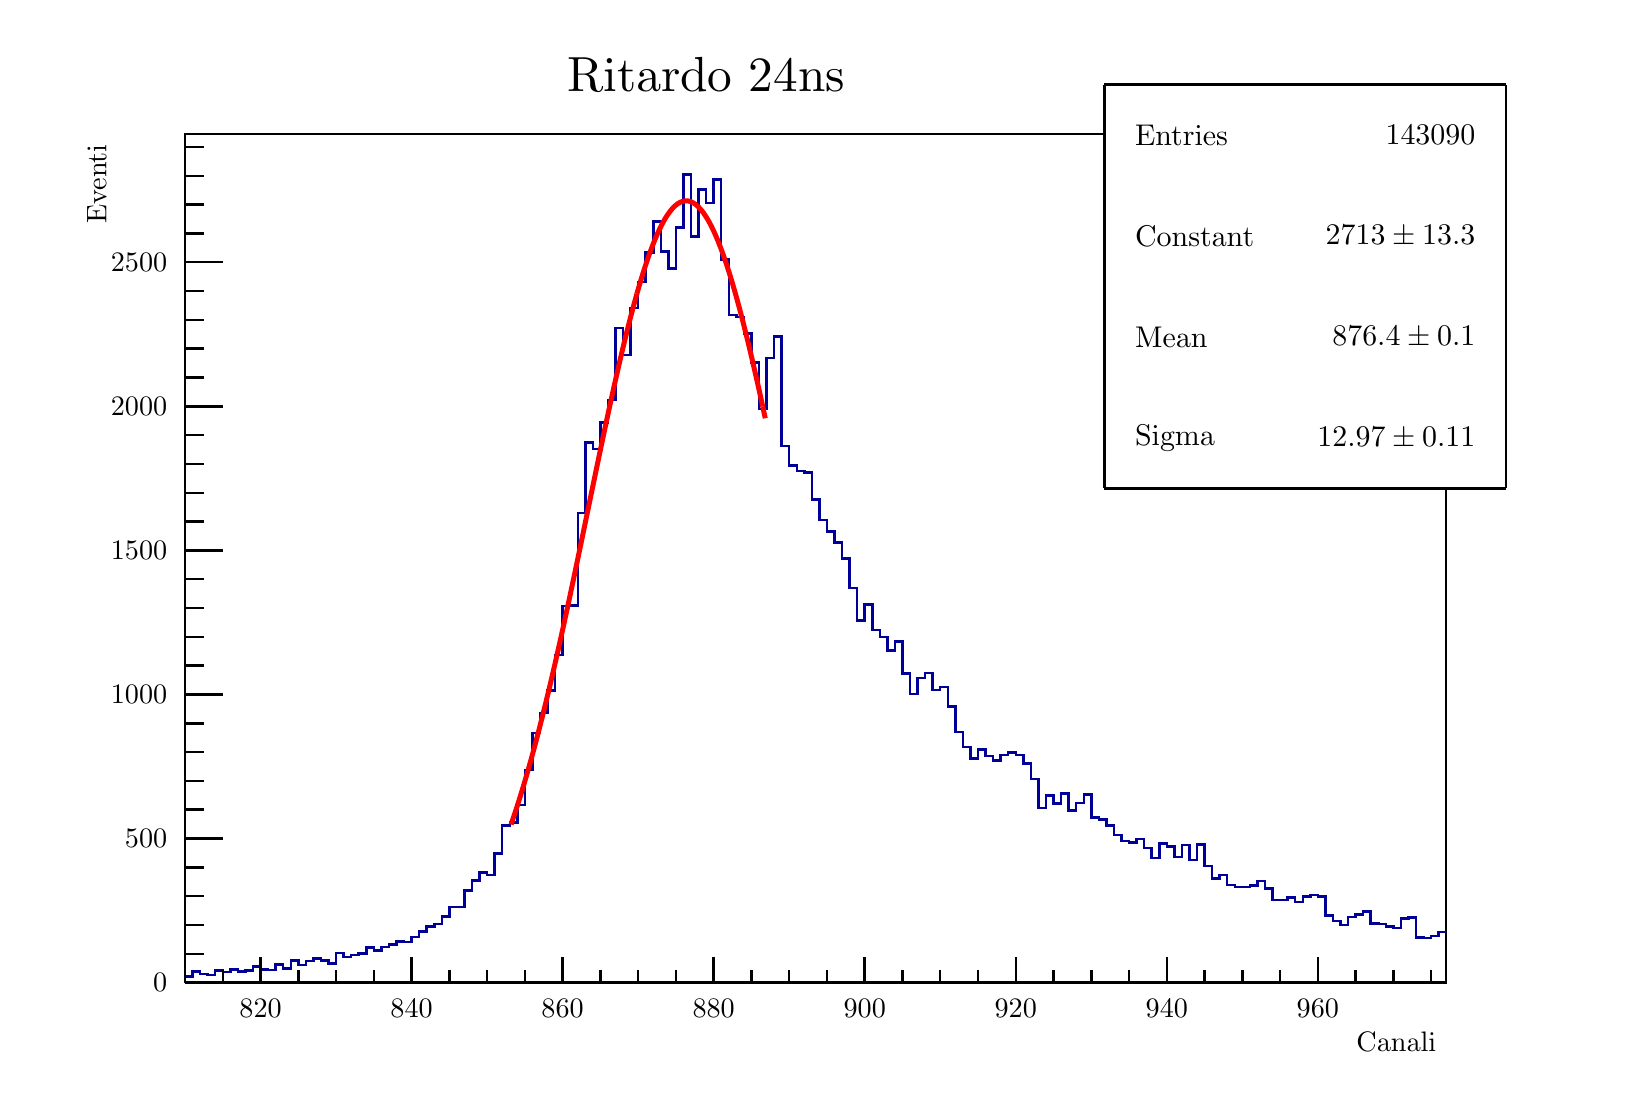
\begin{tikzpicture}
\pgfdeclareplotmark{cross} {
\pgfpathmoveto{\pgfpoint{-0.3\pgfplotmarksize}{\pgfplotmarksize}}
\pgfpathlineto{\pgfpoint{+0.3\pgfplotmarksize}{\pgfplotmarksize}}
\pgfpathlineto{\pgfpoint{+0.3\pgfplotmarksize}{0.3\pgfplotmarksize}}
\pgfpathlineto{\pgfpoint{+1\pgfplotmarksize}{0.3\pgfplotmarksize}}
\pgfpathlineto{\pgfpoint{+1\pgfplotmarksize}{-0.3\pgfplotmarksize}}
\pgfpathlineto{\pgfpoint{+0.3\pgfplotmarksize}{-0.3\pgfplotmarksize}}
\pgfpathlineto{\pgfpoint{+0.3\pgfplotmarksize}{-1.\pgfplotmarksize}}
\pgfpathlineto{\pgfpoint{-0.3\pgfplotmarksize}{-1.\pgfplotmarksize}}
\pgfpathlineto{\pgfpoint{-0.3\pgfplotmarksize}{-0.3\pgfplotmarksize}}
\pgfpathlineto{\pgfpoint{-1.\pgfplotmarksize}{-0.3\pgfplotmarksize}}
\pgfpathlineto{\pgfpoint{-1.\pgfplotmarksize}{0.3\pgfplotmarksize}}
\pgfpathlineto{\pgfpoint{-0.3\pgfplotmarksize}{0.3\pgfplotmarksize}}
\pgfpathclose
\pgfusepathqstroke
}
\pgfdeclareplotmark{cross*} {
\pgfpathmoveto{\pgfpoint{-0.3\pgfplotmarksize}{\pgfplotmarksize}}
\pgfpathlineto{\pgfpoint{+0.3\pgfplotmarksize}{\pgfplotmarksize}}
\pgfpathlineto{\pgfpoint{+0.3\pgfplotmarksize}{0.3\pgfplotmarksize}}
\pgfpathlineto{\pgfpoint{+1\pgfplotmarksize}{0.3\pgfplotmarksize}}
\pgfpathlineto{\pgfpoint{+1\pgfplotmarksize}{-0.3\pgfplotmarksize}}
\pgfpathlineto{\pgfpoint{+0.3\pgfplotmarksize}{-0.3\pgfplotmarksize}}
\pgfpathlineto{\pgfpoint{+0.3\pgfplotmarksize}{-1.\pgfplotmarksize}}
\pgfpathlineto{\pgfpoint{-0.3\pgfplotmarksize}{-1.\pgfplotmarksize}}
\pgfpathlineto{\pgfpoint{-0.3\pgfplotmarksize}{-0.3\pgfplotmarksize}}
\pgfpathlineto{\pgfpoint{-1.\pgfplotmarksize}{-0.3\pgfplotmarksize}}
\pgfpathlineto{\pgfpoint{-1.\pgfplotmarksize}{0.3\pgfplotmarksize}}
\pgfpathlineto{\pgfpoint{-0.3\pgfplotmarksize}{0.3\pgfplotmarksize}}
\pgfpathclose
\pgfusepathqfillstroke
}
\pgfdeclareplotmark{newstar} {
\pgfpathmoveto{\pgfqpoint{0pt}{\pgfplotmarksize}}
\pgfpathlineto{\pgfqpointpolar{44}{0.5\pgfplotmarksize}}
\pgfpathlineto{\pgfqpointpolar{18}{\pgfplotmarksize}}
\pgfpathlineto{\pgfqpointpolar{-20}{0.5\pgfplotmarksize}}
\pgfpathlineto{\pgfqpointpolar{-54}{\pgfplotmarksize}}
\pgfpathlineto{\pgfqpointpolar{-90}{0.5\pgfplotmarksize}}
\pgfpathlineto{\pgfqpointpolar{234}{\pgfplotmarksize}}
\pgfpathlineto{\pgfqpointpolar{198}{0.5\pgfplotmarksize}}
\pgfpathlineto{\pgfqpointpolar{162}{\pgfplotmarksize}}
\pgfpathlineto{\pgfqpointpolar{134}{0.5\pgfplotmarksize}}
\pgfpathclose
\pgfusepathqstroke
}
\pgfdeclareplotmark{newstar*} {
\pgfpathmoveto{\pgfqpoint{0pt}{\pgfplotmarksize}}
\pgfpathlineto{\pgfqpointpolar{44}{0.5\pgfplotmarksize}}
\pgfpathlineto{\pgfqpointpolar{18}{\pgfplotmarksize}}
\pgfpathlineto{\pgfqpointpolar{-20}{0.5\pgfplotmarksize}}
\pgfpathlineto{\pgfqpointpolar{-54}{\pgfplotmarksize}}
\pgfpathlineto{\pgfqpointpolar{-90}{0.5\pgfplotmarksize}}
\pgfpathlineto{\pgfqpointpolar{234}{\pgfplotmarksize}}
\pgfpathlineto{\pgfqpointpolar{198}{0.5\pgfplotmarksize}}
\pgfpathlineto{\pgfqpointpolar{162}{\pgfplotmarksize}}
\pgfpathlineto{\pgfqpointpolar{134}{0.5\pgfplotmarksize}}
\pgfpathclose
\pgfusepathqfillstroke
}
\definecolor{c}{rgb}{1,1,1};
\draw [color=c, fill=c] (0,0) rectangle (20,13.4957);
\draw [color=c, fill=c] (1.9914,1.37536) rectangle (18.0086,12.149);
\definecolor{c}{rgb}{0,0,0};
\draw [c,line width=0.9] (1.9914,1.37536) -- (1.9914,12.149) -- (18.0086,12.149) -- (18.0086,1.37536) -- (1.9914,1.37536);
\definecolor{c}{rgb}{1,1,1};
\draw [color=c, fill=c] (1.9914,1.37536) rectangle (18.0086,12.149);
\definecolor{c}{rgb}{0,0,0};
\draw [c,line width=0.9] (1.9914,1.37536) -- (1.9914,12.149) -- (18.0086,12.149) -- (18.0086,1.37536) -- (1.9914,1.37536);
\definecolor{c}{rgb}{0,0,0.6};
\draw [c,line width=0.9] (1.9914,1.4522) -- (2.08732,1.4522) -- (2.08732,1.51807) -- (2.18323,1.51807) -- (2.18323,1.48514) -- (2.27914,1.48514) -- (2.27914,1.4705) -- (2.37505,1.4705) -- (2.37505,1.52905) -- (2.47096,1.52905) -- (2.47096,1.50709) --
 (2.56687,1.50709) -- (2.56687,1.54003) -- (2.66278,1.54003) -- (2.66278,1.51807) -- (2.75869,1.51807) -- (2.75869,1.52905) -- (2.85461,1.52905) -- (2.85461,1.57662) -- (2.95052,1.57662) -- (2.95052,1.54003) -- (3.04643,1.54003) -- (3.04643,1.53637)
 -- (3.14234,1.53637) -- (3.14234,1.60223) -- (3.23825,1.60223) -- (3.23825,1.55466) -- (3.33416,1.55466) -- (3.33416,1.65712) -- (3.43007,1.65712) -- (3.43007,1.59857) -- (3.52599,1.59857) -- (3.52599,1.6498) -- (3.6219,1.6498) -- (3.6219,1.67908)
 -- (3.71781,1.67908) -- (3.71781,1.65346) -- (3.81372,1.65346) -- (3.81372,1.61687) -- (3.90963,1.61687) -- (3.90963,1.75226) -- (4.00554,1.75226) -- (4.00554,1.70103) -- (4.10145,1.70103) -- (4.10145,1.72665) -- (4.19736,1.72665) --
 (4.19736,1.74495) -- (4.29328,1.74495) -- (4.29328,1.82179) -- (4.38919,1.82179) -- (4.38919,1.78154) -- (4.4851,1.78154) -- (4.4851,1.82911) -- (4.58101,1.82911) -- (4.58101,1.85838) -- (4.67692,1.85838) -- (4.67692,1.89863) -- (4.77283,1.89863) --
 (4.77283,1.88766) -- (4.86874,1.88766) -- (4.86874,1.95718) -- (4.96466,1.95718) -- (4.96466,2.02671) -- (5.06057,2.02671) -- (5.06057,2.08892) -- (5.15648,2.08892) -- (5.15648,2.11819) -- (5.25239,2.11819) -- (5.25239,2.21333) -- (5.3483,2.21333)
 -- (5.3483,2.33409) -- (5.44421,2.33409) -- (5.44421,2.33775) -- (5.54012,2.33775) -- (5.54012,2.54267) -- (5.63603,2.54267) -- (5.63603,2.67074) -- (5.73195,2.67074) -- (5.73195,2.7732) -- (5.82786,2.7732) -- (5.82786,2.74393) -- (5.92377,2.74393)
 -- (5.92377,3.01471) -- (6.01968,3.01471) -- (6.01968,3.37332) -- (6.11559,3.37332) -- (6.11559,3.40626) -- (6.2115,3.40626) -- (6.2115,3.63313) -- (6.30741,3.63313) -- (6.30741,4.0759) -- (6.40333,4.0759) -- (6.40333,4.54795) -- (6.49924,4.54795)
 -- (6.49924,4.79678) -- (6.59515,4.79678) -- (6.59515,5.0822) -- (6.69106,5.0822) -- (6.69106,5.53595) -- (6.78697,5.53595) -- (6.78697,6.15803) -- (6.88288,6.15803) -- (6.88288,6.16169) -- (6.97879,6.16169) -- (6.97879,7.33998) -- (7.0747,7.33998)
 -- (7.0747,8.23284) -- (7.17062,8.23284) -- (7.17062,8.14868) -- (7.26653,8.14868) -- (7.26653,8.48899) -- (7.36244,8.48899) -- (7.36244,8.77441) -- (7.45835,8.77441) -- (7.45835,9.68923) -- (7.55426,9.68923) -- (7.55426,9.34526) --
 (7.65017,9.34526) -- (7.65017,9.94172) -- (7.74608,9.94172) -- (7.74608,10.2711) -- (7.842,10.2711) -- (7.842,10.648) -- (7.93791,10.648) -- (7.93791,11.0395) -- (8.03382,11.0395) -- (8.03382,10.6626) -- (8.12973,10.6626) -- (8.12973,10.4467) --
 (8.22564,10.4467) -- (8.22564,10.9627) -- (8.32155,10.9627) -- (8.32155,11.636) -- (8.41746,11.636) -- (8.41746,10.8492) -- (8.51337,10.8492) -- (8.51337,11.4493) -- (8.60929,11.4493) -- (8.60929,11.2737) -- (8.7052,11.2737) -- (8.7052,11.5774) --
 (8.80111,11.5774) -- (8.80111,10.5565) -- (8.89702,10.5565) -- (8.89702,9.8539) -- (8.99293,9.8539) -- (8.99293,9.82828) -- (9.08884,9.82828) -- (9.08884,9.61605) -- (9.18475,9.61605) -- (9.18475,9.25012) -- (9.28067,9.25012) -- (9.28067,8.66098) --
 (9.37658,8.66098) -- (9.37658,9.30867) -- (9.47249,9.30867) -- (9.47249,9.57945) -- (9.5684,9.57945) -- (9.5684,8.18893) -- (9.66431,8.18893) -- (9.66431,7.94376) -- (9.76022,7.94376) -- (9.76022,7.87423) -- (9.85613,7.87423) -- (9.85613,7.85594) --
 (9.95204,7.85594) -- (9.95204,7.51196) -- (10.048,7.51196) -- (10.048,7.2485) -- (10.1439,7.2485) -- (10.1439,7.10578) -- (10.2398,7.10578) -- (10.2398,6.96307) -- (10.3357,6.96307) -- (10.3357,6.76181) -- (10.4316,6.76181) -- (10.4316,6.38857) --
 (10.5275,6.38857) -- (10.5275,5.97507) -- (10.6234,5.97507) -- (10.6234,6.17999) -- (10.7193,6.17999) -- (10.7193,5.85065) -- (10.8152,5.85065) -- (10.8152,5.76283) -- (10.9112,5.76283) -- (10.9112,5.59084) -- (11.0071,5.59084) -- (11.0071,5.70428)
 -- (11.103,5.70428) -- (11.103,5.2981) -- (11.1989,5.2981) -- (11.1989,5.04195) -- (11.2948,5.04195) -- (11.2948,5.24321) -- (11.3907,5.24321) -- (11.3907,5.30542) -- (11.4866,5.30542) -- (11.4866,5.08952) -- (11.5825,5.08952) -- (11.5825,5.12612)
 -- (11.6784,5.12612) -- (11.6784,4.88094) -- (11.7744,4.88094) -- (11.7744,4.55893) -- (11.8703,4.55893) -- (11.8703,4.36865) -- (11.9662,4.36865) -- (11.9662,4.22227) -- (12.0621,4.22227) -- (12.0621,4.33571) -- (12.158,4.33571) -- (12.158,4.25521)
 -- (12.2539,4.25521) -- (12.2539,4.19666) -- (12.3498,4.19666) -- (12.3498,4.26253) -- (12.4457,4.26253) -- (12.4457,4.29546) -- (12.5416,4.29546) -- (12.5416,4.26619) -- (12.6376,4.26619) -- (12.6376,4.15641) -- (12.7335,4.15641) --
 (12.7335,3.95881) -- (12.8294,3.95881) -- (12.8294,3.59288) -- (12.9253,3.59288) -- (12.9253,3.75023) -- (13.0212,3.75023) -- (13.0212,3.65143) -- (13.1171,3.65143) -- (13.1171,3.77584) -- (13.213,3.77584) -- (13.213,3.5636) -- (13.3089,3.5636) --
 (13.3089,3.65509) -- (13.4049,3.65509) -- (13.4049,3.76121) -- (13.5008,3.76121) -- (13.5008,3.47212) -- (13.5967,3.47212) -- (13.5967,3.44651) -- (13.6926,3.44651) -- (13.6926,3.37332) -- (13.7885,3.37332) -- (13.7885,3.25257) -- (13.8844,3.25257)
 -- (13.8844,3.17206) -- (13.9803,3.17206) -- (13.9803,3.15377) -- (14.0762,3.15377) -- (14.0762,3.19768) -- (14.1721,3.19768) -- (14.1721,3.08424) -- (14.2681,3.08424) -- (14.2681,2.95617) -- (14.364,2.95617) -- (14.364,3.13913) -- (14.4599,3.13913)
 -- (14.4599,3.1062) -- (14.5558,3.1062) -- (14.5558,2.9708) -- (14.6517,2.9708) -- (14.6517,3.12449) -- (14.7476,3.12449) -- (14.7476,2.93055) -- (14.8435,2.93055) -- (14.8435,3.13181) -- (14.9394,3.13181) -- (14.9394,2.85736) -- (15.0353,2.85736)
 -- (15.0353,2.70002) -- (15.1313,2.70002) -- (15.1313,2.74027) -- (15.2272,2.74027) -- (15.2272,2.61219) -- (15.3231,2.61219) -- (15.3231,2.59024) -- (15.419,2.59024) -- (15.419,2.59024) -- (15.5149,2.59024) -- (15.5149,2.60853) -- (15.6108,2.60853)
 -- (15.6108,2.66342) -- (15.7067,2.66342) -- (15.7067,2.56828) -- (15.8026,2.56828) -- (15.8026,2.42191) -- (15.8985,2.42191) -- (15.8985,2.42191) -- (15.9945,2.42191) -- (15.9945,2.4585) -- (16.0904,2.4585) -- (16.0904,2.39996) -- (16.1863,2.39996)
 -- (16.1863,2.46582) -- (16.2822,2.46582) -- (16.2822,2.48778) -- (16.3781,2.48778) -- (16.3781,2.46948) -- (16.474,2.46948) -- (16.474,2.22797) -- (16.5699,2.22797) -- (16.5699,2.15478) -- (16.6658,2.15478) -- (16.6658,2.10721) -- (16.7617,2.10721)
 -- (16.7617,2.20967) -- (16.8577,2.20967) -- (16.8577,2.23895) -- (16.9536,2.23895) -- (16.9536,2.27554) -- (17.0495,2.27554) -- (17.0495,2.12551) -- (17.1454,2.12551) -- (17.1454,2.12185) -- (17.2413,2.12185) -- (17.2413,2.08526) --
 (17.3372,2.08526) -- (17.3372,2.06696) -- (17.4331,2.06696) -- (17.4331,2.19138) -- (17.529,2.19138) -- (17.529,2.20235) -- (17.625,2.20235) -- (17.625,1.94986) -- (17.7209,1.94986) -- (17.7209,1.94255) -- (17.8168,1.94255) -- (17.8168,1.9645) --
 (17.9127,1.9645) -- (17.9127,2.01573) -- (18.0086,2.01573);
\definecolor{c}{rgb}{1,1,1};
\draw [color=c, fill=c] (13.6676,7.65043) rectangle (18.7679,12.7794);
\definecolor{c}{rgb}{0,0,0};
\draw [c,line width=0.9] (13.6676,7.65043) -- (18.7679,7.65043);
\draw [c,line width=0.9] (18.7679,7.65043) -- (18.7679,12.7794);
\draw [c,line width=0.9] (18.7679,12.7794) -- (13.6676,12.7794);
\draw [c,line width=0.9] (13.6676,12.7794) -- (13.6676,7.65043);
\draw [anchor= west] (13.9226,12.1383) node[scale=1.08185, color=c, rotate=0]{Entries };
\draw [anchor= east] (18.5129,12.1383) node[scale=1.08185, color=c, rotate=0]{ 143090};
\draw [anchor= west] (13.9226,10.856) node[scale=1.08185, color=c, rotate=0]{Constant };
\draw [anchor= east] (18.5129,10.856) node[scale=1.08185, color=c, rotate=0]{$  2713 \pm 13.3$};
\draw [anchor= west] (13.9226,9.57378) node[scale=1.08185, color=c, rotate=0]{Mean     };
\draw [anchor= east] (18.5129,9.57378) node[scale=1.08185, color=c, rotate=0]{$ 876.4 \pm 0.1$};
\draw [anchor= west] (13.9226,8.29155) node[scale=1.08185, color=c, rotate=0]{Sigma    };
\draw [anchor= east] (18.5129,8.29155) node[scale=1.08185, color=c, rotate=0]{$ 12.97 \pm 0.11$};
\definecolor{c}{rgb}{1,0,0};
\draw [c,line width=1.8] (6.1319,3.38318) -- (6.16451,3.47881) -- (6.19712,3.57747) -- (6.22973,3.67919) -- (6.26234,3.78394) -- (6.29495,3.89173) -- (6.32756,4.00253) -- (6.36017,4.11633) -- (6.39278,4.23309) -- (6.42538,4.35279) --
 (6.45799,4.47536) -- (6.4906,4.60076) -- (6.52321,4.72893) -- (6.55582,4.85979) -- (6.58843,4.99328) -- (6.62104,5.1293) -- (6.65365,5.26776) -- (6.68626,5.40855) -- (6.71887,5.55156) -- (6.75148,5.69667) -- (6.78409,5.84375) -- (6.8167,5.99267) --
 (6.84931,6.14327) -- (6.88192,6.2954) -- (6.91453,6.44889) -- (6.94714,6.60358) -- (6.97975,6.75929) -- (7.01236,6.91582) -- (7.04497,7.07299) -- (7.07758,7.23059) -- (7.11019,7.38841) -- (7.1428,7.54625) -- (7.17541,7.70388) -- (7.20802,7.86107) --
 (7.24063,8.01761) -- (7.27324,8.17325) -- (7.30585,8.32776) -- (7.33846,8.48089) -- (7.37107,8.63241) -- (7.40368,8.78206) -- (7.43629,8.92962) -- (7.4689,9.07481) -- (7.50151,9.21741) -- (7.53412,9.35715) -- (7.56673,9.49381) -- (7.59934,9.62714)
 -- (7.63195,9.75689) -- (7.66456,9.88283) -- (7.69717,10.0047) -- (7.72978,10.1224);
\draw [c,line width=1.8] (7.72978,10.1224) -- (7.76239,10.2355) -- (7.795,10.344) -- (7.82761,10.4475) -- (7.86022,10.5459) -- (7.89283,10.6391) -- (7.92544,10.7267) -- (7.95805,10.8087) -- (7.99066,10.8849) -- (8.02327,10.9551) -- (8.05588,11.0192)
 -- (8.08849,11.077) -- (8.1211,11.1285) -- (8.15371,11.1735) -- (8.18632,11.212) -- (8.21893,11.2438) -- (8.25154,11.269) -- (8.28415,11.2874) -- (8.31676,11.299) -- (8.34937,11.3037) -- (8.38198,11.3017) -- (8.41459,11.2929) -- (8.4472,11.2772) --
 (8.4798,11.2548) -- (8.51241,11.2257) -- (8.54502,11.1899) -- (8.57763,11.1475) -- (8.61024,11.0986) -- (8.64285,11.0433) -- (8.67546,10.9817) -- (8.70807,10.914) -- (8.74068,10.8402) -- (8.77329,10.7605) -- (8.8059,10.6751) -- (8.83851,10.5842) --
 (8.87112,10.4879) -- (8.90373,10.3864) -- (8.93634,10.2799) -- (8.96895,10.1686) -- (9.00156,10.0528) -- (9.03417,9.93258) -- (9.06678,9.80824) -- (9.09939,9.68) -- (9.132,9.54809) -- (9.16461,9.41275) -- (9.19722,9.27422) -- (9.22983,9.13274) --
 (9.26244,8.98857) -- (9.29505,8.84194) -- (9.32766,8.6931);
\draw [c,line width=1.8] (9.32766,8.6931) -- (9.36027,8.54231);
\definecolor{c}{rgb}{0,0,0};
\draw [c,line width=0.9] (1.9914,1.37536) -- (18.0086,1.37536);
\draw [anchor= east] (18.0086,0.619599) node[scale=1.01821, color=c, rotate=0]{Canali};
\draw [c,line width=0.9] (2.95052,1.6996) -- (2.95052,1.37536);
\draw [c,line width=0.9] (3.43007,1.53748) -- (3.43007,1.37536);
\draw [c,line width=0.9] (3.90963,1.53748) -- (3.90963,1.37536);
\draw [c,line width=0.9] (4.38919,1.53748) -- (4.38919,1.37536);
\draw [c,line width=0.9] (4.86874,1.6996) -- (4.86874,1.37536);
\draw [c,line width=0.9] (5.3483,1.53748) -- (5.3483,1.37536);
\draw [c,line width=0.9] (5.82786,1.53748) -- (5.82786,1.37536);
\draw [c,line width=0.9] (6.30741,1.53748) -- (6.30741,1.37536);
\draw [c,line width=0.9] (6.78697,1.6996) -- (6.78697,1.37536);
\draw [c,line width=0.9] (7.26653,1.53748) -- (7.26653,1.37536);
\draw [c,line width=0.9] (7.74608,1.53748) -- (7.74608,1.37536);
\draw [c,line width=0.9] (8.22564,1.53748) -- (8.22564,1.37536);
\draw [c,line width=0.9] (8.7052,1.6996) -- (8.7052,1.37536);
\draw [c,line width=0.9] (9.18475,1.53748) -- (9.18475,1.37536);
\draw [c,line width=0.9] (9.66431,1.53748) -- (9.66431,1.37536);
\draw [c,line width=0.9] (10.1439,1.53748) -- (10.1439,1.37536);
\draw [c,line width=0.9] (10.6234,1.6996) -- (10.6234,1.37536);
\draw [c,line width=0.9] (11.103,1.53748) -- (11.103,1.37536);
\draw [c,line width=0.9] (11.5825,1.53748) -- (11.5825,1.37536);
\draw [c,line width=0.9] (12.0621,1.53748) -- (12.0621,1.37536);
\draw [c,line width=0.9] (12.5416,1.6996) -- (12.5416,1.37536);
\draw [c,line width=0.9] (13.0212,1.53748) -- (13.0212,1.37536);
\draw [c,line width=0.9] (13.5008,1.53748) -- (13.5008,1.37536);
\draw [c,line width=0.9] (13.9803,1.53748) -- (13.9803,1.37536);
\draw [c,line width=0.9] (14.4599,1.6996) -- (14.4599,1.37536);
\draw [c,line width=0.9] (14.9394,1.53748) -- (14.9394,1.37536);
\draw [c,line width=0.9] (15.419,1.53748) -- (15.419,1.37536);
\draw [c,line width=0.9] (15.8985,1.53748) -- (15.8985,1.37536);
\draw [c,line width=0.9] (16.3781,1.6996) -- (16.3781,1.37536);
\draw [c,line width=0.9] (2.95052,1.6996) -- (2.95052,1.37536);
\draw [c,line width=0.9] (2.47096,1.53748) -- (2.47096,1.37536);
\draw [c,line width=0.9] (1.9914,1.53748) -- (1.9914,1.37536);
\draw [c,line width=0.9] (16.3781,1.6996) -- (16.3781,1.37536);
\draw [c,line width=0.9] (16.8577,1.53748) -- (16.8577,1.37536);
\draw [c,line width=0.9] (17.3372,1.53748) -- (17.3372,1.37536);
\draw [c,line width=0.9] (17.8168,1.53748) -- (17.8168,1.37536);
\draw [anchor=base] (2.95052,0.93) node[scale=1.01821, color=c, rotate=0]{820};
\draw [anchor=base] (4.86874,0.93) node[scale=1.01821, color=c, rotate=0]{840};
\draw [anchor=base] (6.78697,0.93) node[scale=1.01821, color=c, rotate=0]{860};
\draw [anchor=base] (8.7052,0.93) node[scale=1.01821, color=c, rotate=0]{880};
\draw [anchor=base] (10.6234,0.93) node[scale=1.01821, color=c, rotate=0]{900};
\draw [anchor=base] (12.5416,0.93) node[scale=1.01821, color=c, rotate=0]{920};
\draw [anchor=base] (14.4599,0.93) node[scale=1.01821, color=c, rotate=0]{940};
\draw [anchor=base] (16.3781,0.93) node[scale=1.01821, color=c, rotate=0]{960};
\draw [c,line width=0.9] (1.9914,1.37536) -- (1.9914,12.149);
\draw [anchor= east] (0.871404,12.149) node[scale=1.01821, color=c, rotate=90]{Eventi};
\draw [c,line width=0.9] (2.47038,1.37536) -- (1.9914,1.37536);
\draw [c,line width=0.9] (2.23089,1.74129) -- (1.9914,1.74129);
\draw [c,line width=0.9] (2.23089,2.10721) -- (1.9914,2.10721);
\draw [c,line width=0.9] (2.23089,2.47314) -- (1.9914,2.47314);
\draw [c,line width=0.9] (2.23089,2.83907) -- (1.9914,2.83907);
\draw [c,line width=0.9] (2.47038,3.205) -- (1.9914,3.205);
\draw [c,line width=0.9] (2.23089,3.57092) -- (1.9914,3.57092);
\draw [c,line width=0.9] (2.23089,3.93685) -- (1.9914,3.93685);
\draw [c,line width=0.9] (2.23089,4.30278) -- (1.9914,4.30278);
\draw [c,line width=0.9] (2.23089,4.66871) -- (1.9914,4.66871);
\draw [c,line width=0.9] (2.47038,5.03463) -- (1.9914,5.03463);
\draw [c,line width=0.9] (2.23089,5.40056) -- (1.9914,5.40056);
\draw [c,line width=0.9] (2.23089,5.76649) -- (1.9914,5.76649);
\draw [c,line width=0.9] (2.23089,6.13242) -- (1.9914,6.13242);
\draw [c,line width=0.9] (2.23089,6.49834) -- (1.9914,6.49834);
\draw [c,line width=0.9] (2.47038,6.86427) -- (1.9914,6.86427);
\draw [c,line width=0.9] (2.23089,7.2302) -- (1.9914,7.2302);
\draw [c,line width=0.9] (2.23089,7.59613) -- (1.9914,7.59613);
\draw [c,line width=0.9] (2.23089,7.96205) -- (1.9914,7.96205);
\draw [c,line width=0.9] (2.23089,8.32798) -- (1.9914,8.32798);
\draw [c,line width=0.9] (2.47038,8.69391) -- (1.9914,8.69391);
\draw [c,line width=0.9] (2.23089,9.05984) -- (1.9914,9.05984);
\draw [c,line width=0.9] (2.23089,9.42576) -- (1.9914,9.42576);
\draw [c,line width=0.9] (2.23089,9.79169) -- (1.9914,9.79169);
\draw [c,line width=0.9] (2.23089,10.1576) -- (1.9914,10.1576);
\draw [c,line width=0.9] (2.47038,10.5235) -- (1.9914,10.5235);
\draw [c,line width=0.9] (2.47038,10.5235) -- (1.9914,10.5235);
\draw [c,line width=0.9] (2.23089,10.8895) -- (1.9914,10.8895);
\draw [c,line width=0.9] (2.23089,11.2554) -- (1.9914,11.2554);
\draw [c,line width=0.9] (2.23089,11.6213) -- (1.9914,11.6213);
\draw [c,line width=0.9] (2.23089,11.9873) -- (1.9914,11.9873);
\draw [anchor= east] (1.8914,1.37536) node[scale=1.01821, color=c, rotate=0]{0};
\draw [anchor= east] (1.8914,3.205) node[scale=1.01821, color=c, rotate=0]{500};
\draw [anchor= east] (1.8914,5.03463) node[scale=1.01821, color=c, rotate=0]{1000};
\draw [anchor= east] (1.8914,6.86427) node[scale=1.01821, color=c, rotate=0]{1500};
\draw [anchor= east] (1.8914,8.69391) node[scale=1.01821, color=c, rotate=0]{2000};
\draw [anchor= east] (1.8914,10.5235) node[scale=1.01821, color=c, rotate=0]{2500};
\definecolor{c}{rgb}{1,1,1};
\draw [color=c, fill=c] (13.6676,7.65043) rectangle (18.7679,12.7794);
\definecolor{c}{rgb}{0,0,0};
\draw [c,line width=0.9] (13.6676,7.65043) -- (18.7679,7.65043);
\draw [c,line width=0.9] (18.7679,7.65043) -- (18.7679,12.7794);
\draw [c,line width=0.9] (18.7679,12.7794) -- (13.6676,12.7794);
\draw [c,line width=0.9] (13.6676,12.7794) -- (13.6676,7.65043);
\draw [anchor= west] (13.9226,12.1383) node[scale=1.08185, color=c, rotate=0]{Entries };
\draw [anchor= east] (18.5129,12.1383) node[scale=1.08185, color=c, rotate=0]{ 143090};
\draw [anchor= west] (13.9226,10.856) node[scale=1.08185, color=c, rotate=0]{Constant };
\draw [anchor= east] (18.5129,10.856) node[scale=1.08185, color=c, rotate=0]{$  2713 \pm 13.3$};
\draw [anchor= west] (13.9226,9.57378) node[scale=1.08185, color=c, rotate=0]{Mean     };
\draw [anchor= east] (18.5129,9.57378) node[scale=1.08185, color=c, rotate=0]{$ 876.4 \pm 0.1$};
\draw [anchor= west] (13.9226,8.29155) node[scale=1.08185, color=c, rotate=0]{Sigma    };
\draw [anchor= east] (18.5129,8.29155) node[scale=1.08185, color=c, rotate=0]{$ 12.97 \pm 0.11$};
\draw (8.61032,12.9083) node[scale=1.78187, color=c, rotate=0]{Ritardo 24ns};
\end{tikzpicture}

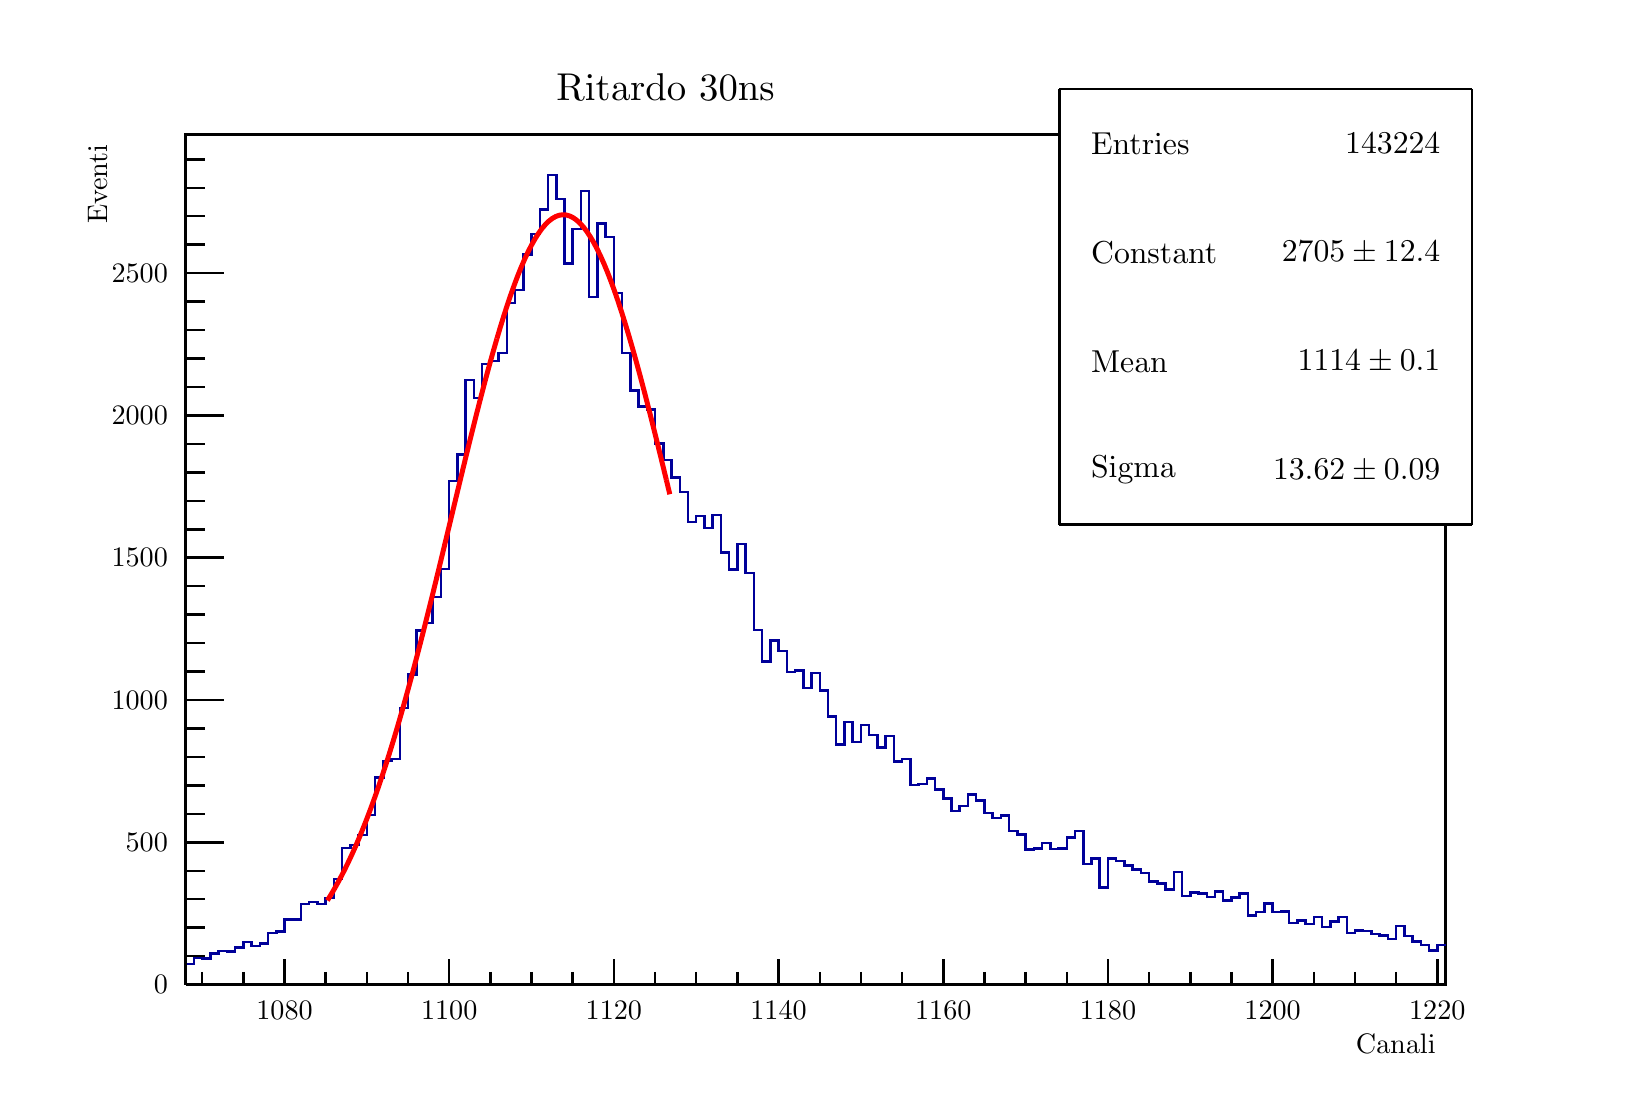
\begin{tikzpicture}
\pgfdeclareplotmark{cross} {
\pgfpathmoveto{\pgfpoint{-0.3\pgfplotmarksize}{\pgfplotmarksize}}
\pgfpathlineto{\pgfpoint{+0.3\pgfplotmarksize}{\pgfplotmarksize}}
\pgfpathlineto{\pgfpoint{+0.3\pgfplotmarksize}{0.3\pgfplotmarksize}}
\pgfpathlineto{\pgfpoint{+1\pgfplotmarksize}{0.3\pgfplotmarksize}}
\pgfpathlineto{\pgfpoint{+1\pgfplotmarksize}{-0.3\pgfplotmarksize}}
\pgfpathlineto{\pgfpoint{+0.3\pgfplotmarksize}{-0.3\pgfplotmarksize}}
\pgfpathlineto{\pgfpoint{+0.3\pgfplotmarksize}{-1.\pgfplotmarksize}}
\pgfpathlineto{\pgfpoint{-0.3\pgfplotmarksize}{-1.\pgfplotmarksize}}
\pgfpathlineto{\pgfpoint{-0.3\pgfplotmarksize}{-0.3\pgfplotmarksize}}
\pgfpathlineto{\pgfpoint{-1.\pgfplotmarksize}{-0.3\pgfplotmarksize}}
\pgfpathlineto{\pgfpoint{-1.\pgfplotmarksize}{0.3\pgfplotmarksize}}
\pgfpathlineto{\pgfpoint{-0.3\pgfplotmarksize}{0.3\pgfplotmarksize}}
\pgfpathclose
\pgfusepathqstroke
}
\pgfdeclareplotmark{cross*} {
\pgfpathmoveto{\pgfpoint{-0.3\pgfplotmarksize}{\pgfplotmarksize}}
\pgfpathlineto{\pgfpoint{+0.3\pgfplotmarksize}{\pgfplotmarksize}}
\pgfpathlineto{\pgfpoint{+0.3\pgfplotmarksize}{0.3\pgfplotmarksize}}
\pgfpathlineto{\pgfpoint{+1\pgfplotmarksize}{0.3\pgfplotmarksize}}
\pgfpathlineto{\pgfpoint{+1\pgfplotmarksize}{-0.3\pgfplotmarksize}}
\pgfpathlineto{\pgfpoint{+0.3\pgfplotmarksize}{-0.3\pgfplotmarksize}}
\pgfpathlineto{\pgfpoint{+0.3\pgfplotmarksize}{-1.\pgfplotmarksize}}
\pgfpathlineto{\pgfpoint{-0.3\pgfplotmarksize}{-1.\pgfplotmarksize}}
\pgfpathlineto{\pgfpoint{-0.3\pgfplotmarksize}{-0.3\pgfplotmarksize}}
\pgfpathlineto{\pgfpoint{-1.\pgfplotmarksize}{-0.3\pgfplotmarksize}}
\pgfpathlineto{\pgfpoint{-1.\pgfplotmarksize}{0.3\pgfplotmarksize}}
\pgfpathlineto{\pgfpoint{-0.3\pgfplotmarksize}{0.3\pgfplotmarksize}}
\pgfpathclose
\pgfusepathqfillstroke
}
\pgfdeclareplotmark{newstar} {
\pgfpathmoveto{\pgfqpoint{0pt}{\pgfplotmarksize}}
\pgfpathlineto{\pgfqpointpolar{44}{0.5\pgfplotmarksize}}
\pgfpathlineto{\pgfqpointpolar{18}{\pgfplotmarksize}}
\pgfpathlineto{\pgfqpointpolar{-20}{0.5\pgfplotmarksize}}
\pgfpathlineto{\pgfqpointpolar{-54}{\pgfplotmarksize}}
\pgfpathlineto{\pgfqpointpolar{-90}{0.5\pgfplotmarksize}}
\pgfpathlineto{\pgfqpointpolar{234}{\pgfplotmarksize}}
\pgfpathlineto{\pgfqpointpolar{198}{0.5\pgfplotmarksize}}
\pgfpathlineto{\pgfqpointpolar{162}{\pgfplotmarksize}}
\pgfpathlineto{\pgfqpointpolar{134}{0.5\pgfplotmarksize}}
\pgfpathclose
\pgfusepathqstroke
}
\pgfdeclareplotmark{newstar*} {
\pgfpathmoveto{\pgfqpoint{0pt}{\pgfplotmarksize}}
\pgfpathlineto{\pgfqpointpolar{44}{0.5\pgfplotmarksize}}
\pgfpathlineto{\pgfqpointpolar{18}{\pgfplotmarksize}}
\pgfpathlineto{\pgfqpointpolar{-20}{0.5\pgfplotmarksize}}
\pgfpathlineto{\pgfqpointpolar{-54}{\pgfplotmarksize}}
\pgfpathlineto{\pgfqpointpolar{-90}{0.5\pgfplotmarksize}}
\pgfpathlineto{\pgfqpointpolar{234}{\pgfplotmarksize}}
\pgfpathlineto{\pgfqpointpolar{198}{0.5\pgfplotmarksize}}
\pgfpathlineto{\pgfqpointpolar{162}{\pgfplotmarksize}}
\pgfpathlineto{\pgfqpointpolar{134}{0.5\pgfplotmarksize}}
\pgfpathclose
\pgfusepathqfillstroke
}
\definecolor{c}{rgb}{1,1,1};
\draw [color=c, fill=c] (0,0) rectangle (20,13.4957);
\draw [color=c, fill=c] (2,1.34957) rectangle (18,12.1461);
\definecolor{c}{rgb}{0,0,0};
\draw [c,line width=0.9] (2,1.34957) -- (2,12.1461) -- (18,12.1461) -- (18,1.34957) -- (2,1.34957);
\definecolor{c}{rgb}{1,1,1};
\draw [color=c, fill=c] (2,1.34957) rectangle (18,12.1461);
\definecolor{c}{rgb}{0,0,0};
\draw [c,line width=0.9] (2,1.34957) -- (2,12.1461) -- (18,12.1461) -- (18,1.34957) -- (2,1.34957);
\definecolor{c}{rgb}{0,0,0.6};
\draw [c,line width=0.9] (2,1.61341) -- (2.10458,1.61341) -- (2.10458,1.69292) -- (2.20915,1.69292) -- (2.20915,1.67846) -- (2.31373,1.67846) -- (2.31373,1.74713) -- (2.4183,1.74713) -- (2.4183,1.77966) -- (2.52288,1.77966) -- (2.52288,1.76882) --
 (2.62745,1.76882) -- (2.62745,1.81942) -- (2.73203,1.81942) -- (2.73203,1.8917) -- (2.8366,1.8917) -- (2.8366,1.83749) -- (2.94118,1.83749) -- (2.94118,1.87002) -- (3.04575,1.87002) -- (3.04575,2.00374) -- (3.15033,2.00374) -- (3.15033,2.02181) --
 (3.2549,2.02181) -- (3.2549,2.17361) -- (3.35948,2.17361) -- (3.35948,2.17723) -- (3.46405,2.17723) -- (3.46405,2.37239) -- (3.56863,2.37239) -- (3.56863,2.40131) -- (3.6732,2.40131) -- (3.6732,2.37601) -- (3.77778,2.37601) -- (3.77778,2.45191) --
 (3.88235,2.45191) -- (3.88235,2.69406) -- (3.98693,2.69406) -- (3.98693,3.08439) -- (4.0915,3.08439) -- (4.0915,3.12054) -- (4.19608,3.12054) -- (4.19608,3.25065) -- (4.30065,3.25065) -- (4.30065,3.50364) -- (4.40523,3.50364) -- (4.40523,3.98072) --
 (4.5098,3.98072) -- (4.5098,4.18673) -- (4.61438,4.18673) -- (4.61438,4.21564) -- (4.71895,4.21564) -- (4.71895,4.86259) -- (4.82353,4.86259) -- (4.82353,5.28545) -- (4.9281,5.28545) -- (4.9281,5.84565) -- (5.03268,5.84565) -- (5.03268,5.93962) --
 (5.13726,5.93962) -- (5.13726,6.27213) -- (5.24183,6.27213) -- (5.24183,6.62632) -- (5.34641,6.62632) -- (5.34641,7.74311) -- (5.45098,7.74311) -- (5.45098,8.07924) -- (5.55556,8.07924) -- (5.55556,9.02978) -- (5.66013,9.02978) -- (5.66013,8.79847)
 -- (5.76471,8.79847) -- (5.76471,9.23217) -- (5.86928,9.23217) -- (5.86928,9.26831) -- (5.97386,9.26831) -- (5.97386,9.37313) -- (6.07843,9.37313) -- (6.07843,10.0056) -- (6.18301,10.0056) -- (6.18301,10.1719) -- (6.28758,10.1719) --
 (6.28758,10.6236) -- (6.39216,10.6236) -- (6.39216,10.8803) -- (6.49673,10.8803) -- (6.49673,11.1911) -- (6.60131,11.1911) -- (6.60131,11.632) -- (6.70588,11.632) -- (6.70588,11.3284) -- (6.81046,11.3284) -- (6.81046,10.508) -- (6.91503,10.508) --
 (6.91503,10.9453) -- (7.01961,10.9453) -- (7.01961,11.426) -- (7.12418,11.426) -- (7.12418,10.0815) -- (7.22876,10.0815) -- (7.22876,11.014) -- (7.33333,11.014) -- (7.33333,10.8441) -- (7.43791,10.8441) -- (7.43791,10.1321) -- (7.54248,10.1321) --
 (7.54248,9.36951) -- (7.64706,9.36951) -- (7.64706,8.89244) -- (7.75163,8.89244) -- (7.75163,8.69365) -- (7.85621,8.69365) -- (7.85621,8.6539) -- (7.96078,8.6539) -- (7.96078,8.22019) -- (8.06536,8.22019) -- (8.06536,8.01418) -- (8.16993,8.01418) --
 (8.16993,7.7901) -- (8.27451,7.7901) -- (8.27451,7.60577) -- (8.37908,7.60577) -- (8.37908,7.22267) -- (8.48366,7.22267) -- (8.48366,7.29857) -- (8.58823,7.29857) -- (8.58823,7.14677) -- (8.69281,7.14677) -- (8.69281,7.31302) -- (8.79739,7.31302) --
 (8.79739,6.83595) -- (8.90196,6.83595) -- (8.90196,6.61909) -- (9.00654,6.61909) -- (9.00654,6.94437) -- (9.11111,6.94437) -- (9.11111,6.57934) -- (9.21569,6.57934) -- (9.21569,5.85288) -- (9.32026,5.85288) -- (9.32026,5.45532) -- (9.42484,5.45532)
 -- (9.42484,5.72277) -- (9.52941,5.72277) -- (9.52941,5.58904) -- (9.63399,5.58904) -- (9.63399,5.31798) -- (9.73856,5.31798) -- (9.73856,5.33966) -- (9.84314,5.33966) -- (9.84314,5.1192) -- (9.94771,5.1192) -- (9.94771,5.30713) -- (10.0523,5.30713)
 -- (10.0523,5.08667) -- (10.1569,5.08667) -- (10.1569,4.75416) -- (10.2614,4.75416) -- (10.2614,4.39997) -- (10.366,4.39997) -- (10.366,4.68188) -- (10.4706,4.68188) -- (10.4706,4.42888) -- (10.5752,4.42888) -- (10.5752,4.64935) -- (10.6797,4.64935)
 -- (10.6797,4.51924) -- (10.7843,4.51924) -- (10.7843,4.36021) -- (10.8889,4.36021) -- (10.8889,4.50839) -- (10.9935,4.50839) -- (10.9935,4.18311) -- (11.098,4.18311) -- (11.098,4.21564) -- (11.2026,4.21564) -- (11.2026,3.88313) -- (11.3072,3.88313)
 -- (11.3072,3.89759) -- (11.4118,3.89759) -- (11.4118,3.96988) -- (11.5163,3.96988) -- (11.5163,3.82892) -- (11.6209,3.82892) -- (11.6209,3.71327) -- (11.7255,3.71327) -- (11.7255,3.55424) -- (11.8301,3.55424) -- (11.8301,3.6193) -- (11.9346,3.6193)
 -- (11.9346,3.76387) -- (12.0392,3.76387) -- (12.0392,3.68797) -- (12.1438,3.68797) -- (12.1438,3.52894) -- (12.2484,3.52894) -- (12.2484,3.4675) -- (12.3529,3.4675) -- (12.3529,3.49641) -- (12.4575,3.49641) -- (12.4575,3.29763) -- (12.5621,3.29763)
 -- (12.5621,3.25788) -- (12.6667,3.25788) -- (12.6667,3.06632) -- (12.7712,3.06632) -- (12.7712,3.07716) -- (12.8758,3.07716) -- (12.8758,3.14945) -- (12.9804,3.14945) -- (12.9804,3.06994) -- (13.085,3.06994) -- (13.085,3.07716) -- (13.1895,3.07716)
 -- (13.1895,3.21812) -- (13.2941,3.21812) -- (13.2941,3.30125) -- (13.3987,3.30125) -- (13.3987,2.882) -- (13.5033,2.882) -- (13.5033,2.95067) -- (13.6078,2.95067) -- (13.6078,2.58202) -- (13.7124,2.58202) -- (13.7124,2.95428) -- (13.817,2.95428) --
 (13.817,2.92175) -- (13.9216,2.92175) -- (13.9216,2.86031) -- (14.0261,2.86031) -- (14.0261,2.81333) -- (14.1307,2.81333) -- (14.1307,2.76996) -- (14.2353,2.76996) -- (14.2353,2.66153) -- (14.3399,2.66153) -- (14.3399,2.63623) -- (14.4444,2.63623)
 -- (14.4444,2.55672) -- (14.549,2.55672) -- (14.549,2.77718) -- (14.6536,2.77718) -- (14.6536,2.47359) -- (14.7582,2.47359) -- (14.7582,2.52058) -- (14.8627,2.52058) -- (14.8627,2.50973) -- (14.9673,2.50973) -- (14.9673,2.46275) -- (15.0719,2.46275)
 -- (15.0719,2.53503) -- (15.1765,2.53503) -- (15.1765,2.41938) -- (15.281,2.41938) -- (15.281,2.45552) -- (15.3856,2.45552) -- (15.3856,2.50973) -- (15.4902,2.50973) -- (15.4902,2.22782) -- (15.5948,2.22782) -- (15.5948,2.27119) -- (15.6993,2.27119)
 -- (15.6993,2.37962) -- (15.8039,2.37962) -- (15.8039,2.27119) -- (15.9085,2.27119) -- (15.9085,2.27842) -- (16.0131,2.27842) -- (16.0131,2.13385) -- (16.1176,2.13385) -- (16.1176,2.16638) -- (16.2222,2.16638) -- (16.2222,2.1194) -- (16.3268,2.1194)
 -- (16.3268,2.20614) -- (16.4314,2.20614) -- (16.4314,2.07964) -- (16.5359,2.07964) -- (16.5359,2.14831) -- (16.6405,2.14831) -- (16.6405,2.20975) -- (16.7451,2.20975) -- (16.7451,2.00374) -- (16.8497,2.00374) -- (16.8497,2.03627) --
 (16.9542,2.03627) -- (16.9542,2.02904) -- (17.0588,2.02904) -- (17.0588,1.98929) -- (17.1634,1.98929) -- (17.1634,1.97483) -- (17.268,1.97483) -- (17.268,1.92784) -- (17.3725,1.92784) -- (17.3725,2.0941) -- (17.4771,2.0941) -- (17.4771,1.96399) --
 (17.5817,1.96399) -- (17.5817,1.89532) -- (17.6863,1.89532) -- (17.6863,1.85195) -- (17.7908,1.85195) -- (17.7908,1.78328) -- (17.8954,1.78328) -- (17.8954,1.85195) -- (18,1.85195);
\definecolor{c}{rgb}{1,1,1};
\draw [color=c, fill=c] (13.0946,7.19198) rectangle (18.3381,12.7221);
\definecolor{c}{rgb}{0,0,0};
\draw [c,line width=0.9] (13.0946,7.19198) -- (18.3381,7.19198);
\draw [c,line width=0.9] (18.3381,7.19198) -- (18.3381,12.7221);
\draw [c,line width=0.9] (18.3381,12.7221) -- (13.0946,12.7221);
\draw [c,line width=0.9] (13.0946,12.7221) -- (13.0946,7.19198);
\draw [anchor= west] (13.3567,12.0308) node[scale=1.14549, color=c, rotate=0]{Entries };
\draw [anchor= east] (18.0759,12.0308) node[scale=1.14549, color=c, rotate=0]{ 143224};
\draw [anchor= west] (13.3567,10.6483) node[scale=1.14549, color=c, rotate=0]{Constant };
\draw [anchor= east] (18.0759,10.6483) node[scale=1.14549, color=c, rotate=0]{$  2705 \pm 12.4$};
\draw [anchor= west] (13.3567,9.26576) node[scale=1.14549, color=c, rotate=0]{Mean     };
\draw [anchor= east] (18.0759,9.26576) node[scale=1.14549, color=c, rotate=0]{$  1114 \pm 0.1$};
\draw [anchor= west] (13.3567,7.88324) node[scale=1.14549, color=c, rotate=0]{Sigma    };
\draw [anchor= east] (18.0759,7.88324) node[scale=1.14549, color=c, rotate=0]{$ 13.62 \pm 0.09$};
\definecolor{c}{rgb}{1,0,0};
\draw [c,line width=1.8] (3.79974,2.41852) -- (3.84366,2.48965) -- (3.88758,2.56436) -- (3.9315,2.64274) -- (3.97543,2.72486) -- (4.01935,2.81081) -- (4.06327,2.90065) -- (4.10719,2.99446) -- (4.15111,3.09227) -- (4.19503,3.19415) --
 (4.23895,3.30012) -- (4.28288,3.41022) -- (4.3268,3.52447) -- (4.37072,3.64286) -- (4.41464,3.7654) -- (4.45856,3.89207) -- (4.50248,4.02284) -- (4.54641,4.15765) -- (4.59033,4.29647) -- (4.63425,4.4392) -- (4.67817,4.58576) -- (4.72209,4.73605) --
 (4.76601,4.88996) -- (4.80993,5.04733) -- (4.85386,5.20803) -- (4.89778,5.37189) -- (4.9417,5.53871) -- (4.98562,5.7083) -- (5.02954,5.88045) -- (5.07346,6.05491) -- (5.11739,6.23145) -- (5.16131,6.40979) -- (5.20523,6.58965) -- (5.24915,6.77076) --
 (5.29307,6.95278) -- (5.33699,7.13541) -- (5.38092,7.31831) -- (5.42484,7.50113) -- (5.46876,7.68353) -- (5.51268,7.86513) -- (5.5566,8.04556) -- (5.60052,8.22444) -- (5.64444,8.40139) -- (5.68837,8.57602) -- (5.73229,8.74792) -- (5.77621,8.91671)
 -- (5.82013,9.08199) -- (5.86405,9.24337) -- (5.90797,9.40045) -- (5.9519,9.55285);
\draw [c,line width=1.8] (5.9519,9.55285) -- (5.99582,9.70018) -- (6.03974,9.84207) -- (6.08366,9.97816) -- (6.12758,10.1081) -- (6.1715,10.2315) -- (6.21543,10.3481) -- (6.25935,10.4576) -- (6.30327,10.5596) -- (6.34719,10.6539) -- (6.39111,10.7403)
 -- (6.43503,10.8184) -- (6.47895,10.8881) -- (6.52288,10.9492) -- (6.5668,11.0015) -- (6.61072,11.0448) -- (6.65464,11.079) -- (6.69856,11.1041) -- (6.74248,11.12) -- (6.78641,11.1266) -- (6.83033,11.1239) -- (6.87425,11.1118) -- (6.91817,11.0906)
 -- (6.96209,11.0601) -- (7.00601,11.0205) -- (7.04993,10.9719) -- (7.09386,10.9145) -- (7.13778,10.8483) -- (7.1817,10.7737) -- (7.22562,10.6907) -- (7.26954,10.5997) -- (7.31346,10.5008) -- (7.35739,10.3944) -- (7.40131,10.2807) --
 (7.44523,10.1601) -- (7.48915,10.0328) -- (7.53307,9.89922) -- (7.57699,9.75969) -- (7.62091,9.61457) -- (7.66484,9.46423) -- (7.70876,9.30904) -- (7.75268,9.1494) -- (7.7966,8.98569) -- (7.84052,8.81831) -- (7.88444,8.64765) -- (7.92837,8.4741) --
 (7.97229,8.29807) -- (8.01621,8.11994) -- (8.06013,7.9401) -- (8.10405,7.75894);
\draw [c,line width=1.8] (8.10405,7.75894) -- (8.14797,7.57683);
\definecolor{c}{rgb}{0,0,0};
\draw [c,line width=0.9] (2,1.34957) -- (18,1.34957);
\draw [anchor= east] (18,0.593811) node[scale=1.01821, color=c, rotate=0]{Canali};
\draw [c,line width=0.9] (3.2549,1.67347) -- (3.2549,1.34957);
\draw [c,line width=0.9] (3.77778,1.51152) -- (3.77778,1.34957);
\draw [c,line width=0.9] (4.30065,1.51152) -- (4.30065,1.34957);
\draw [c,line width=0.9] (4.82353,1.51152) -- (4.82353,1.34957);
\draw [c,line width=0.9] (5.34641,1.67347) -- (5.34641,1.34957);
\draw [c,line width=0.9] (5.86928,1.51152) -- (5.86928,1.34957);
\draw [c,line width=0.9] (6.39216,1.51152) -- (6.39216,1.34957);
\draw [c,line width=0.9] (6.91503,1.51152) -- (6.91503,1.34957);
\draw [c,line width=0.9] (7.43791,1.67347) -- (7.43791,1.34957);
\draw [c,line width=0.9] (7.96078,1.51152) -- (7.96078,1.34957);
\draw [c,line width=0.9] (8.48366,1.51152) -- (8.48366,1.34957);
\draw [c,line width=0.9] (9.00654,1.51152) -- (9.00654,1.34957);
\draw [c,line width=0.9] (9.52941,1.67347) -- (9.52941,1.34957);
\draw [c,line width=0.9] (10.0523,1.51152) -- (10.0523,1.34957);
\draw [c,line width=0.9] (10.5752,1.51152) -- (10.5752,1.34957);
\draw [c,line width=0.9] (11.098,1.51152) -- (11.098,1.34957);
\draw [c,line width=0.9] (11.6209,1.67347) -- (11.6209,1.34957);
\draw [c,line width=0.9] (12.1438,1.51152) -- (12.1438,1.34957);
\draw [c,line width=0.9] (12.6667,1.51152) -- (12.6667,1.34957);
\draw [c,line width=0.9] (13.1895,1.51152) -- (13.1895,1.34957);
\draw [c,line width=0.9] (13.7124,1.67347) -- (13.7124,1.34957);
\draw [c,line width=0.9] (14.2353,1.51152) -- (14.2353,1.34957);
\draw [c,line width=0.9] (14.7582,1.51152) -- (14.7582,1.34957);
\draw [c,line width=0.9] (15.281,1.51152) -- (15.281,1.34957);
\draw [c,line width=0.9] (15.8039,1.67347) -- (15.8039,1.34957);
\draw [c,line width=0.9] (16.3268,1.51152) -- (16.3268,1.34957);
\draw [c,line width=0.9] (16.8497,1.51152) -- (16.8497,1.34957);
\draw [c,line width=0.9] (17.3725,1.51152) -- (17.3725,1.34957);
\draw [c,line width=0.9] (17.8954,1.67347) -- (17.8954,1.34957);
\draw [c,line width=0.9] (3.2549,1.67347) -- (3.2549,1.34957);
\draw [c,line width=0.9] (2.73203,1.51152) -- (2.73203,1.34957);
\draw [c,line width=0.9] (2.20915,1.51152) -- (2.20915,1.34957);
\draw [c,line width=0.9] (17.8954,1.67347) -- (17.8954,1.34957);
\draw [anchor=base] (3.2549,0.904212) node[scale=1.01821, color=c, rotate=0]{1080};
\draw [anchor=base] (5.34641,0.904212) node[scale=1.01821, color=c, rotate=0]{1100};
\draw [anchor=base] (7.43791,0.904212) node[scale=1.01821, color=c, rotate=0]{1120};
\draw [anchor=base] (9.52941,0.904212) node[scale=1.01821, color=c, rotate=0]{1140};
\draw [anchor=base] (11.6209,0.904212) node[scale=1.01821, color=c, rotate=0]{1160};
\draw [anchor=base] (13.7124,0.904212) node[scale=1.01821, color=c, rotate=0]{1180};
\draw [anchor=base] (15.8039,0.904212) node[scale=1.01821, color=c, rotate=0]{1200};
\draw [anchor=base] (17.8954,0.904212) node[scale=1.01821, color=c, rotate=0]{1220};
\draw [c,line width=0.9] (2,1.34957) -- (2,12.1461);
\draw [anchor= east] (0.88,12.1461) node[scale=1.01821, color=c, rotate=90]{Eventi};
\draw [c,line width=0.9] (2.48,1.34957) -- (2,1.34957);
\draw [c,line width=0.9] (2.24,1.71099) -- (2,1.71099);
\draw [c,line width=0.9] (2.24,2.07241) -- (2,2.07241);
\draw [c,line width=0.9] (2.24,2.43383) -- (2,2.43383);
\draw [c,line width=0.9] (2.24,2.79526) -- (2,2.79526);
\draw [c,line width=0.9] (2.48,3.15668) -- (2,3.15668);
\draw [c,line width=0.9] (2.24,3.5181) -- (2,3.5181);
\draw [c,line width=0.9] (2.24,3.87952) -- (2,3.87952);
\draw [c,line width=0.9] (2.24,4.24094) -- (2,4.24094);
\draw [c,line width=0.9] (2.24,4.60236) -- (2,4.60236);
\draw [c,line width=0.9] (2.48,4.96378) -- (2,4.96378);
\draw [c,line width=0.9] (2.24,5.32521) -- (2,5.32521);
\draw [c,line width=0.9] (2.24,5.68663) -- (2,5.68663);
\draw [c,line width=0.9] (2.24,6.04805) -- (2,6.04805);
\draw [c,line width=0.9] (2.24,6.40947) -- (2,6.40947);
\draw [c,line width=0.9] (2.48,6.77089) -- (2,6.77089);
\draw [c,line width=0.9] (2.24,7.13231) -- (2,7.13231);
\draw [c,line width=0.9] (2.24,7.49373) -- (2,7.49373);
\draw [c,line width=0.9] (2.24,7.85516) -- (2,7.85516);
\draw [c,line width=0.9] (2.24,8.21658) -- (2,8.21658);
\draw [c,line width=0.9] (2.48,8.578) -- (2,8.578);
\draw [c,line width=0.9] (2.24,8.93942) -- (2,8.93942);
\draw [c,line width=0.9] (2.24,9.30084) -- (2,9.30084);
\draw [c,line width=0.9] (2.24,9.66226) -- (2,9.66226);
\draw [c,line width=0.9] (2.24,10.0237) -- (2,10.0237);
\draw [c,line width=0.9] (2.48,10.3851) -- (2,10.3851);
\draw [c,line width=0.9] (2.48,10.3851) -- (2,10.3851);
\draw [c,line width=0.9] (2.24,10.7465) -- (2,10.7465);
\draw [c,line width=0.9] (2.24,11.1079) -- (2,11.1079);
\draw [c,line width=0.9] (2.24,11.4694) -- (2,11.4694);
\draw [c,line width=0.9] (2.24,11.8308) -- (2,11.8308);
\draw [anchor= east] (1.9,1.34957) node[scale=1.01821, color=c, rotate=0]{0};
\draw [anchor= east] (1.9,3.15668) node[scale=1.01821, color=c, rotate=0]{500};
\draw [anchor= east] (1.9,4.96378) node[scale=1.01821, color=c, rotate=0]{1000};
\draw [anchor= east] (1.9,6.77089) node[scale=1.01821, color=c, rotate=0]{1500};
\draw [anchor= east] (1.9,8.578) node[scale=1.01821, color=c, rotate=0]{2000};
\draw [anchor= east] (1.9,10.3851) node[scale=1.01821, color=c, rotate=0]{2500};
\definecolor{c}{rgb}{1,1,1};
\draw [color=c, fill=c] (13.0946,7.19198) rectangle (18.3381,12.7221);
\definecolor{c}{rgb}{0,0,0};
\draw [c,line width=0.9] (13.0946,7.19198) -- (18.3381,7.19198);
\draw [c,line width=0.9] (18.3381,7.19198) -- (18.3381,12.7221);
\draw [c,line width=0.9] (18.3381,12.7221) -- (13.0946,12.7221);
\draw [c,line width=0.9] (13.0946,12.7221) -- (13.0946,7.19198);
\draw [anchor= west] (13.3567,12.0308) node[scale=1.14549, color=c, rotate=0]{Entries };
\draw [anchor= east] (18.0759,12.0308) node[scale=1.14549, color=c, rotate=0]{ 143224};
\draw [anchor= west] (13.3567,10.6483) node[scale=1.14549, color=c, rotate=0]{Constant };
\draw [anchor= east] (18.0759,10.6483) node[scale=1.14549, color=c, rotate=0]{$  2705 \pm 12.4$};
\draw [anchor= west] (13.3567,9.26576) node[scale=1.14549, color=c, rotate=0]{Mean     };
\draw [anchor= east] (18.0759,9.26576) node[scale=1.14549, color=c, rotate=0]{$  1114 \pm 0.1$};
\draw [anchor= west] (13.3567,7.88324) node[scale=1.14549, color=c, rotate=0]{Sigma    };
\draw [anchor= east] (18.0759,7.88324) node[scale=1.14549, color=c, rotate=0]{$ 13.62 \pm 0.09$};
\draw (8.09456,12.7507) node[scale=1.40004, color=c, rotate=0]{Ritardo 30ns};
\end{tikzpicture}

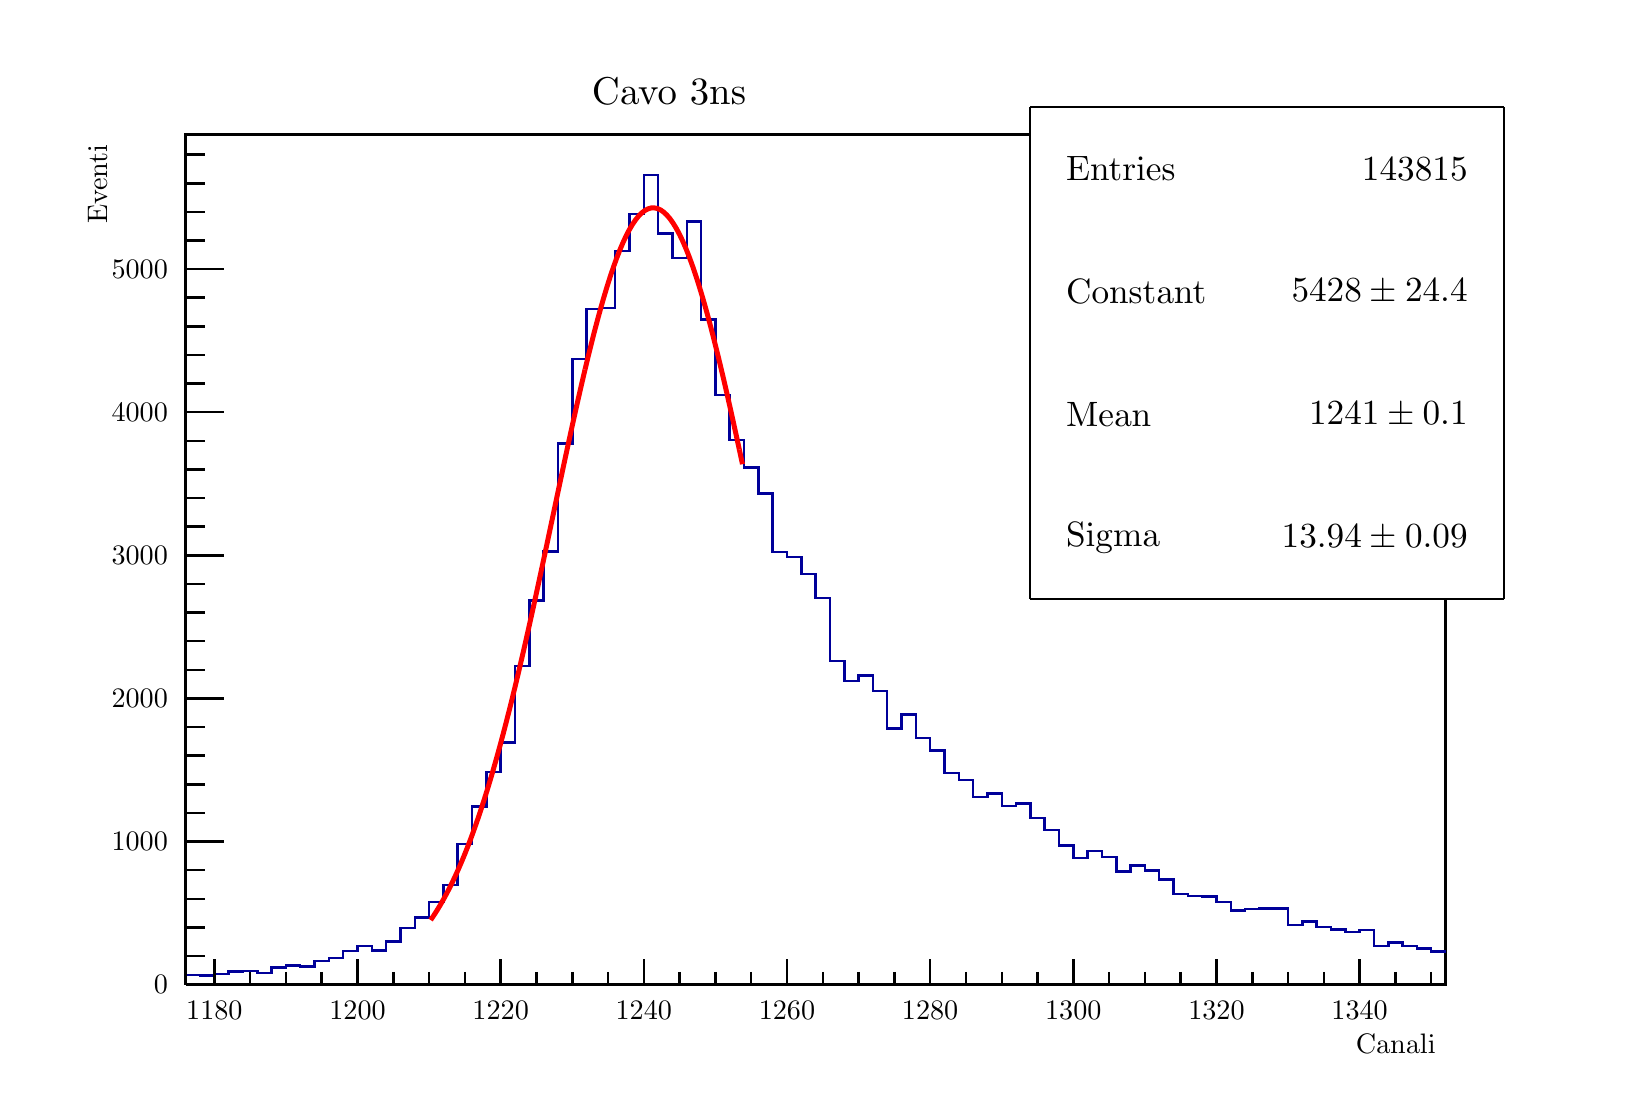
\begin{tikzpicture}
\pgfdeclareplotmark{cross} {
\pgfpathmoveto{\pgfpoint{-0.3\pgfplotmarksize}{\pgfplotmarksize}}
\pgfpathlineto{\pgfpoint{+0.3\pgfplotmarksize}{\pgfplotmarksize}}
\pgfpathlineto{\pgfpoint{+0.3\pgfplotmarksize}{0.3\pgfplotmarksize}}
\pgfpathlineto{\pgfpoint{+1\pgfplotmarksize}{0.3\pgfplotmarksize}}
\pgfpathlineto{\pgfpoint{+1\pgfplotmarksize}{-0.3\pgfplotmarksize}}
\pgfpathlineto{\pgfpoint{+0.3\pgfplotmarksize}{-0.3\pgfplotmarksize}}
\pgfpathlineto{\pgfpoint{+0.3\pgfplotmarksize}{-1.\pgfplotmarksize}}
\pgfpathlineto{\pgfpoint{-0.3\pgfplotmarksize}{-1.\pgfplotmarksize}}
\pgfpathlineto{\pgfpoint{-0.3\pgfplotmarksize}{-0.3\pgfplotmarksize}}
\pgfpathlineto{\pgfpoint{-1.\pgfplotmarksize}{-0.3\pgfplotmarksize}}
\pgfpathlineto{\pgfpoint{-1.\pgfplotmarksize}{0.3\pgfplotmarksize}}
\pgfpathlineto{\pgfpoint{-0.3\pgfplotmarksize}{0.3\pgfplotmarksize}}
\pgfpathclose
\pgfusepathqstroke
}
\pgfdeclareplotmark{cross*} {
\pgfpathmoveto{\pgfpoint{-0.3\pgfplotmarksize}{\pgfplotmarksize}}
\pgfpathlineto{\pgfpoint{+0.3\pgfplotmarksize}{\pgfplotmarksize}}
\pgfpathlineto{\pgfpoint{+0.3\pgfplotmarksize}{0.3\pgfplotmarksize}}
\pgfpathlineto{\pgfpoint{+1\pgfplotmarksize}{0.3\pgfplotmarksize}}
\pgfpathlineto{\pgfpoint{+1\pgfplotmarksize}{-0.3\pgfplotmarksize}}
\pgfpathlineto{\pgfpoint{+0.3\pgfplotmarksize}{-0.3\pgfplotmarksize}}
\pgfpathlineto{\pgfpoint{+0.3\pgfplotmarksize}{-1.\pgfplotmarksize}}
\pgfpathlineto{\pgfpoint{-0.3\pgfplotmarksize}{-1.\pgfplotmarksize}}
\pgfpathlineto{\pgfpoint{-0.3\pgfplotmarksize}{-0.3\pgfplotmarksize}}
\pgfpathlineto{\pgfpoint{-1.\pgfplotmarksize}{-0.3\pgfplotmarksize}}
\pgfpathlineto{\pgfpoint{-1.\pgfplotmarksize}{0.3\pgfplotmarksize}}
\pgfpathlineto{\pgfpoint{-0.3\pgfplotmarksize}{0.3\pgfplotmarksize}}
\pgfpathclose
\pgfusepathqfillstroke
}
\pgfdeclareplotmark{newstar} {
\pgfpathmoveto{\pgfqpoint{0pt}{\pgfplotmarksize}}
\pgfpathlineto{\pgfqpointpolar{44}{0.5\pgfplotmarksize}}
\pgfpathlineto{\pgfqpointpolar{18}{\pgfplotmarksize}}
\pgfpathlineto{\pgfqpointpolar{-20}{0.5\pgfplotmarksize}}
\pgfpathlineto{\pgfqpointpolar{-54}{\pgfplotmarksize}}
\pgfpathlineto{\pgfqpointpolar{-90}{0.5\pgfplotmarksize}}
\pgfpathlineto{\pgfqpointpolar{234}{\pgfplotmarksize}}
\pgfpathlineto{\pgfqpointpolar{198}{0.5\pgfplotmarksize}}
\pgfpathlineto{\pgfqpointpolar{162}{\pgfplotmarksize}}
\pgfpathlineto{\pgfqpointpolar{134}{0.5\pgfplotmarksize}}
\pgfpathclose
\pgfusepathqstroke
}
\pgfdeclareplotmark{newstar*} {
\pgfpathmoveto{\pgfqpoint{0pt}{\pgfplotmarksize}}
\pgfpathlineto{\pgfqpointpolar{44}{0.5\pgfplotmarksize}}
\pgfpathlineto{\pgfqpointpolar{18}{\pgfplotmarksize}}
\pgfpathlineto{\pgfqpointpolar{-20}{0.5\pgfplotmarksize}}
\pgfpathlineto{\pgfqpointpolar{-54}{\pgfplotmarksize}}
\pgfpathlineto{\pgfqpointpolar{-90}{0.5\pgfplotmarksize}}
\pgfpathlineto{\pgfqpointpolar{234}{\pgfplotmarksize}}
\pgfpathlineto{\pgfqpointpolar{198}{0.5\pgfplotmarksize}}
\pgfpathlineto{\pgfqpointpolar{162}{\pgfplotmarksize}}
\pgfpathlineto{\pgfqpointpolar{134}{0.5\pgfplotmarksize}}
\pgfpathclose
\pgfusepathqfillstroke
}
\definecolor{c}{rgb}{1,1,1};
\draw [color=c, fill=c] (0,0) rectangle (20,13.4957);
\draw [color=c, fill=c] (2,1.34957) rectangle (18,12.1461);
\definecolor{c}{rgb}{0,0,0};
\draw [c,line width=0.9] (2,1.34957) -- (2,12.1461) -- (18,12.1461) -- (18,1.34957) -- (2,1.34957);
\definecolor{c}{rgb}{1,1,1};
\draw [color=c, fill=c] (2,1.34957) rectangle (18,12.1461);
\definecolor{c}{rgb}{0,0,0};
\draw [c,line width=0.9] (2,1.34957) -- (2,12.1461) -- (18,12.1461) -- (18,1.34957) -- (2,1.34957);
\definecolor{c}{rgb}{0,0,0.6};
\draw [c,line width=0.9] (2,1.46951) -- (2.18182,1.46951) -- (2.18182,1.46406) -- (2.36364,1.46406) -- (2.36364,1.48587) -- (2.54545,1.48587) -- (2.54545,1.51858) -- (2.72727,1.51858) -- (2.72727,1.5204) -- (2.90909,1.5204) -- (2.90909,1.49859) --
 (3.09091,1.49859) -- (3.09091,1.56947) -- (3.27273,1.56947) -- (3.27273,1.59309) -- (3.45455,1.59309) -- (3.45455,1.58219) -- (3.63636,1.58219) -- (3.63636,1.65125) -- (3.81818,1.65125) -- (3.81818,1.68759) -- (4,1.68759) -- (4,1.77664) --
 (4.18182,1.77664) -- (4.18182,1.83843) -- (4.36364,1.83843) -- (4.36364,1.78209) -- (4.54545,1.78209) -- (4.54545,1.8984) -- (4.72727,1.8984) -- (4.72727,2.06923) -- (4.90909,2.06923) -- (4.90909,2.2019) -- (5.09091,2.2019) -- (5.09091,2.4018) --
 (5.27273,2.4018) -- (5.27273,2.61443) -- (5.45455,2.61443) -- (5.45455,3.13419) -- (5.63636,3.13419) -- (5.63636,3.60851) -- (5.81818,3.60851) -- (5.81818,4.05194) -- (6,4.05194) -- (6,4.42449) -- (6.18182,4.42449) -- (6.18182,5.39312) --
 (6.36364,5.39312) -- (6.36364,6.22728) -- (6.54545,6.22728) -- (6.54545,6.84699) -- (6.72727,6.84699) -- (6.72727,8.21907) -- (6.90909,8.21907) -- (6.90909,9.29311) -- (7.09091,9.29311) -- (7.09091,9.92917) -- (7.27273,9.92917) -- (7.27273,9.94008)
 -- (7.45455,9.94008) -- (7.45455,10.6652) -- (7.63636,10.6652) -- (7.63636,11.1359) -- (7.81818,11.1359) -- (7.81818,11.632) -- (8,11.632) -- (8,10.8869) -- (8.18182,10.8869) -- (8.18182,10.578) -- (8.36364,10.578) -- (8.36364,11.0396) --
 (8.54545,11.0396) -- (8.54545,9.79469) -- (8.72727,9.79469) -- (8.72727,8.84059) -- (8.90909,8.84059) -- (8.90909,8.26632) -- (9.09091,8.26632) -- (9.09091,7.91921) -- (9.27273,7.91921) -- (9.27273,7.58482) -- (9.45455,7.58482) -- (9.45455,6.84335)
 -- (9.63636,6.84335) -- (9.63636,6.78338) -- (9.81818,6.78338) -- (9.81818,6.56712) -- (10,6.56712) -- (10,6.25817) -- (10.1818,6.25817) -- (10.1818,5.45855) -- (10.3636,5.45855) -- (10.3636,5.20776) -- (10.5455,5.20776) -- (10.5455,5.27681) --
 (10.7273,5.27681) -- (10.7273,5.07873) -- (10.9091,5.07873) -- (10.9091,4.60077) -- (11.0909,4.60077) -- (11.0909,4.78068) -- (11.2727,4.78068) -- (11.2727,4.47901) -- (11.4545,4.47901) -- (11.4545,4.32454) -- (11.6364,4.32454) -- (11.6364,4.0374)
 -- (11.8182,4.0374) -- (11.8182,3.94835) -- (12,3.94835) -- (12,3.73209) -- (12.1818,3.73209) -- (12.1818,3.77752) -- (12.3636,3.77752) -- (12.3636,3.6176) -- (12.5455,3.6176) -- (12.5455,3.64667) -- (12.7273,3.64667) -- (12.7273,3.46494) --
 (12.9091,3.46494) -- (12.9091,3.3141) -- (13.0909,3.3141) -- (13.0909,3.11783) -- (13.2727,3.11783) -- (13.2727,2.95791) -- (13.4545,2.95791) -- (13.4545,3.04877) -- (13.6364,3.04877) -- (13.6364,2.97244) -- (13.8182,2.97244) -- (13.8182,2.78889) --
 (14,2.78889) -- (14,2.85977) -- (14.1818,2.85977) -- (14.1818,2.80161) -- (14.3636,2.80161) -- (14.3636,2.68712) -- (14.5455,2.68712) -- (14.5455,2.49994) -- (14.7273,2.49994) -- (14.7273,2.47268) -- (14.9091,2.47268) -- (14.9091,2.46723) --
 (15.0909,2.46723) -- (15.0909,2.4018) -- (15.2727,2.4018) -- (15.2727,2.29095) -- (15.4545,2.29095) -- (15.4545,2.3073) -- (15.6364,2.3073) -- (15.6364,2.31639) -- (15.8182,2.31639) -- (15.8182,2.31457) -- (16,2.31457) -- (16,2.10376) --
 (16.1818,2.10376) -- (16.1818,2.15283) -- (16.3636,2.15283) -- (16.3636,2.07832) -- (16.5455,2.07832) -- (16.5455,2.05106) -- (16.7273,2.05106) -- (16.7273,2.02016) -- (16.9091,2.02016) -- (16.9091,2.04197) -- (17.0909,2.04197) -- (17.0909,1.84207)
 -- (17.2727,1.84207) -- (17.2727,1.88568) -- (17.4545,1.88568) -- (17.4545,1.84207) -- (17.6364,1.84207) -- (17.6364,1.81117) -- (17.8182,1.81117) -- (17.8182,1.77301) -- (18,1.77301);
\definecolor{c}{rgb}{1,1,1};
\draw [color=c, fill=c] (12.7221,6.24642) rectangle (18.7393,12.4928);
\definecolor{c}{rgb}{0,0,0};
\draw [c,line width=0.9] (12.7221,6.24642) -- (18.7393,6.24642);
\draw [c,line width=0.9] (18.7393,6.24642) -- (18.7393,12.4928);
\draw [c,line width=0.9] (18.7393,12.4928) -- (12.7221,12.4928);
\draw [c,line width=0.9] (12.7221,12.4928) -- (12.7221,6.24642);
\draw [anchor= west] (13.0229,11.712) node[scale=1.27276, color=c, rotate=0]{Entries };
\draw [anchor= east] (18.4384,11.712) node[scale=1.27276, color=c, rotate=0]{ 143815};
\draw [anchor= west] (13.0229,10.1504) node[scale=1.27276, color=c, rotate=0]{Constant };
\draw [anchor= east] (18.4384,10.1504) node[scale=1.27276, color=c, rotate=0]{$  5428 \pm 24.4$};
\draw [anchor= west] (13.0229,8.58883) node[scale=1.27276, color=c, rotate=0]{Mean     };
\draw [anchor= east] (18.4384,8.58883) node[scale=1.27276, color=c, rotate=0]{$  1241 \pm 0.1$};
\draw [anchor= west] (13.0229,7.02722) node[scale=1.27276, color=c, rotate=0]{Sigma    };
\draw [anchor= east] (18.4384,7.02722) node[scale=1.27276, color=c, rotate=0]{$ 13.94 \pm 0.09$};
\definecolor{c}{rgb}{1,0,0};
\draw [c,line width=1.8] (5.11091,2.16911) -- (5.15091,2.22848) -- (5.19091,2.2912) -- (5.23091,2.3574) -- (5.27091,2.42718) -- (5.31091,2.50064) -- (5.35091,2.57788) -- (5.39091,2.659) -- (5.43091,2.74408) -- (5.47091,2.83322) -- (5.51091,2.92648)
 -- (5.55091,3.02393) -- (5.59091,3.12563) -- (5.63091,3.23163) -- (5.67091,3.34197) -- (5.71091,3.45668) -- (5.75091,3.57577) -- (5.79091,3.69925) -- (5.83091,3.82711) -- (5.87091,3.95932) -- (5.91091,4.09585) -- (5.95091,4.23664) --
 (5.99091,4.38163) -- (6.03091,4.53072) -- (6.07091,4.68382) -- (6.11091,4.84081) -- (6.15091,5.00154) -- (6.19091,5.16587) -- (6.23091,5.33362) -- (6.27091,5.50459) -- (6.31091,5.67859) -- (6.35091,5.85538) -- (6.39091,6.03472) -- (6.43091,6.21634)
 -- (6.47091,6.39996) -- (6.51091,6.58529) -- (6.55091,6.77201) -- (6.59091,6.95979) -- (6.63091,7.1483) -- (6.67091,7.33717) -- (6.71091,7.52602) -- (6.75091,7.71449) -- (6.79091,7.90217) -- (6.83091,8.08866) -- (6.87091,8.27356) --
 (6.91091,8.45644) -- (6.95091,8.63688) -- (6.99091,8.81446) -- (7.03091,8.98874) -- (7.07091,9.15931);
\draw [c,line width=1.8] (7.07091,9.15931) -- (7.11091,9.32572) -- (7.15091,9.48757) -- (7.19091,9.64443) -- (7.23091,9.79589) -- (7.27091,9.94154) -- (7.31091,10.081) -- (7.35091,10.2139) -- (7.39091,10.3398) -- (7.43091,10.4584) --
 (7.47091,10.5694) -- (7.51091,10.6725) -- (7.55091,10.7673) -- (7.59091,10.8536) -- (7.63091,10.9312) -- (7.67091,10.9997) -- (7.71091,11.0591) -- (7.75091,11.1091) -- (7.79091,11.1495) -- (7.83091,11.1803) -- (7.87091,11.2014) -- (7.91091,11.2128)
 -- (7.95091,11.2142) -- (7.99091,11.2059) -- (8.03091,11.1877) -- (8.07091,11.1598) -- (8.11091,11.1222) -- (8.15091,11.0751) -- (8.19091,11.0186) -- (8.23091,10.9528) -- (8.27091,10.8779) -- (8.31091,10.7942) -- (8.35091,10.7019) --
 (8.39091,10.6013) -- (8.43091,10.4927) -- (8.47091,10.3763) -- (8.51091,10.2525) -- (8.55091,10.1217) -- (8.59091,9.98421) -- (8.63091,9.84038) -- (8.67091,9.69063) -- (8.71091,9.53536) -- (8.75091,9.37497) -- (8.79091,9.20988) -- (8.83091,9.04052)
 -- (8.87091,8.86731) -- (8.91091,8.69068) -- (8.95091,8.51106) -- (8.99091,8.32887) -- (9.03091,8.14454);
\draw [c,line width=1.8] (9.03091,8.14454) -- (9.07091,7.95848);
\definecolor{c}{rgb}{0,0,0};
\draw [c,line width=0.9] (2,1.34957) -- (18,1.34957);
\draw [anchor= east] (18,0.593811) node[scale=1.01821, color=c, rotate=0]{Canali};
\draw [c,line width=0.9] (2.36364,1.67347) -- (2.36364,1.34957);
\draw [c,line width=0.9] (2.81818,1.51152) -- (2.81818,1.34957);
\draw [c,line width=0.9] (3.27273,1.51152) -- (3.27273,1.34957);
\draw [c,line width=0.9] (3.72727,1.51152) -- (3.72727,1.34957);
\draw [c,line width=0.9] (4.18182,1.67347) -- (4.18182,1.34957);
\draw [c,line width=0.9] (4.63636,1.51152) -- (4.63636,1.34957);
\draw [c,line width=0.9] (5.09091,1.51152) -- (5.09091,1.34957);
\draw [c,line width=0.9] (5.54545,1.51152) -- (5.54545,1.34957);
\draw [c,line width=0.9] (6,1.67347) -- (6,1.34957);
\draw [c,line width=0.9] (6.45455,1.51152) -- (6.45455,1.34957);
\draw [c,line width=0.9] (6.90909,1.51152) -- (6.90909,1.34957);
\draw [c,line width=0.9] (7.36364,1.51152) -- (7.36364,1.34957);
\draw [c,line width=0.9] (7.81818,1.67347) -- (7.81818,1.34957);
\draw [c,line width=0.9] (8.27273,1.51152) -- (8.27273,1.34957);
\draw [c,line width=0.9] (8.72727,1.51152) -- (8.72727,1.34957);
\draw [c,line width=0.9] (9.18182,1.51152) -- (9.18182,1.34957);
\draw [c,line width=0.9] (9.63636,1.67347) -- (9.63636,1.34957);
\draw [c,line width=0.9] (10.0909,1.51152) -- (10.0909,1.34957);
\draw [c,line width=0.9] (10.5455,1.51152) -- (10.5455,1.34957);
\draw [c,line width=0.9] (11,1.51152) -- (11,1.34957);
\draw [c,line width=0.9] (11.4545,1.67347) -- (11.4545,1.34957);
\draw [c,line width=0.9] (11.9091,1.51152) -- (11.9091,1.34957);
\draw [c,line width=0.9] (12.3636,1.51152) -- (12.3636,1.34957);
\draw [c,line width=0.9] (12.8182,1.51152) -- (12.8182,1.34957);
\draw [c,line width=0.9] (13.2727,1.67347) -- (13.2727,1.34957);
\draw [c,line width=0.9] (13.7273,1.51152) -- (13.7273,1.34957);
\draw [c,line width=0.9] (14.1818,1.51152) -- (14.1818,1.34957);
\draw [c,line width=0.9] (14.6364,1.51152) -- (14.6364,1.34957);
\draw [c,line width=0.9] (15.0909,1.67347) -- (15.0909,1.34957);
\draw [c,line width=0.9] (15.5455,1.51152) -- (15.5455,1.34957);
\draw [c,line width=0.9] (16,1.51152) -- (16,1.34957);
\draw [c,line width=0.9] (16.4545,1.51152) -- (16.4545,1.34957);
\draw [c,line width=0.9] (16.9091,1.67347) -- (16.9091,1.34957);
\draw [c,line width=0.9] (2.36364,1.67347) -- (2.36364,1.34957);
\draw [c,line width=0.9] (16.9091,1.67347) -- (16.9091,1.34957);
\draw [c,line width=0.9] (17.3636,1.51152) -- (17.3636,1.34957);
\draw [c,line width=0.9] (17.8182,1.51152) -- (17.8182,1.34957);
\draw [anchor=base] (2.36364,0.904212) node[scale=1.01821, color=c, rotate=0]{1180};
\draw [anchor=base] (4.18182,0.904212) node[scale=1.01821, color=c, rotate=0]{1200};
\draw [anchor=base] (6,0.904212) node[scale=1.01821, color=c, rotate=0]{1220};
\draw [anchor=base] (7.81818,0.904212) node[scale=1.01821, color=c, rotate=0]{1240};
\draw [anchor=base] (9.63636,0.904212) node[scale=1.01821, color=c, rotate=0]{1260};
\draw [anchor=base] (11.4545,0.904212) node[scale=1.01821, color=c, rotate=0]{1280};
\draw [anchor=base] (13.2727,0.904212) node[scale=1.01821, color=c, rotate=0]{1300};
\draw [anchor=base] (15.0909,0.904212) node[scale=1.01821, color=c, rotate=0]{1320};
\draw [anchor=base] (16.9091,0.904212) node[scale=1.01821, color=c, rotate=0]{1340};
\draw [c,line width=0.9] (2,1.34957) -- (2,12.1461);
\draw [anchor= east] (0.88,12.1461) node[scale=1.01821, color=c, rotate=90]{Eventi};
\draw [c,line width=0.9] (2.48,1.34957) -- (2,1.34957);
\draw [c,line width=0.9] (2.24,1.71304) -- (2,1.71304);
\draw [c,line width=0.9] (2.24,2.0765) -- (2,2.0765);
\draw [c,line width=0.9] (2.24,2.43997) -- (2,2.43997);
\draw [c,line width=0.9] (2.24,2.80343) -- (2,2.80343);
\draw [c,line width=0.9] (2.48,3.1669) -- (2,3.1669);
\draw [c,line width=0.9] (2.24,3.53036) -- (2,3.53036);
\draw [c,line width=0.9] (2.24,3.89383) -- (2,3.89383);
\draw [c,line width=0.9] (2.24,4.25729) -- (2,4.25729);
\draw [c,line width=0.9] (2.24,4.62076) -- (2,4.62076);
\draw [c,line width=0.9] (2.48,4.98423) -- (2,4.98423);
\draw [c,line width=0.9] (2.24,5.34769) -- (2,5.34769);
\draw [c,line width=0.9] (2.24,5.71116) -- (2,5.71116);
\draw [c,line width=0.9] (2.24,6.07462) -- (2,6.07462);
\draw [c,line width=0.9] (2.24,6.43809) -- (2,6.43809);
\draw [c,line width=0.9] (2.48,6.80155) -- (2,6.80155);
\draw [c,line width=0.9] (2.24,7.16502) -- (2,7.16502);
\draw [c,line width=0.9] (2.24,7.52848) -- (2,7.52848);
\draw [c,line width=0.9] (2.24,7.89195) -- (2,7.89195);
\draw [c,line width=0.9] (2.24,8.25541) -- (2,8.25541);
\draw [c,line width=0.9] (2.48,8.61888) -- (2,8.61888);
\draw [c,line width=0.9] (2.24,8.98235) -- (2,8.98235);
\draw [c,line width=0.9] (2.24,9.34581) -- (2,9.34581);
\draw [c,line width=0.9] (2.24,9.70928) -- (2,9.70928);
\draw [c,line width=0.9] (2.24,10.0727) -- (2,10.0727);
\draw [c,line width=0.9] (2.48,10.4362) -- (2,10.4362);
\draw [c,line width=0.9] (2.48,10.4362) -- (2,10.4362);
\draw [c,line width=0.9] (2.24,10.7997) -- (2,10.7997);
\draw [c,line width=0.9] (2.24,11.1631) -- (2,11.1631);
\draw [c,line width=0.9] (2.24,11.5266) -- (2,11.5266);
\draw [c,line width=0.9] (2.24,11.8901) -- (2,11.8901);
\draw [anchor= east] (1.9,1.34957) node[scale=1.01821, color=c, rotate=0]{0};
\draw [anchor= east] (1.9,3.1669) node[scale=1.01821, color=c, rotate=0]{1000};
\draw [anchor= east] (1.9,4.98423) node[scale=1.01821, color=c, rotate=0]{2000};
\draw [anchor= east] (1.9,6.80155) node[scale=1.01821, color=c, rotate=0]{3000};
\draw [anchor= east] (1.9,8.61888) node[scale=1.01821, color=c, rotate=0]{4000};
\draw [anchor= east] (1.9,10.4362) node[scale=1.01821, color=c, rotate=0]{5000};
\definecolor{c}{rgb}{1,1,1};
\draw [color=c, fill=c] (12.7221,6.24642) rectangle (18.7393,12.4928);
\definecolor{c}{rgb}{0,0,0};
\draw [c,line width=0.9] (12.7221,6.24642) -- (18.7393,6.24642);
\draw [c,line width=0.9] (18.7393,6.24642) -- (18.7393,12.4928);
\draw [c,line width=0.9] (18.7393,12.4928) -- (12.7221,12.4928);
\draw [c,line width=0.9] (12.7221,12.4928) -- (12.7221,6.24642);
\draw [anchor= west] (13.0229,11.712) node[scale=1.27276, color=c, rotate=0]{Entries };
\draw [anchor= east] (18.4384,11.712) node[scale=1.27276, color=c, rotate=0]{ 143815};
\draw [anchor= west] (13.0229,10.1504) node[scale=1.27276, color=c, rotate=0]{Constant };
\draw [anchor= east] (18.4384,10.1504) node[scale=1.27276, color=c, rotate=0]{$  5428 \pm 24.4$};
\draw [anchor= west] (13.0229,8.58883) node[scale=1.27276, color=c, rotate=0]{Mean     };
\draw [anchor= east] (18.4384,8.58883) node[scale=1.27276, color=c, rotate=0]{$  1241 \pm 0.1$};
\draw [anchor= west] (13.0229,7.02722) node[scale=1.27276, color=c, rotate=0]{Sigma    };
\draw [anchor= east] (18.4384,7.02722) node[scale=1.27276, color=c, rotate=0]{$ 13.94 \pm 0.09$};
\draw (8.13754,12.6934) node[scale=1.40004, color=c, rotate=0]{Cavo 3ns};
\end{tikzpicture}

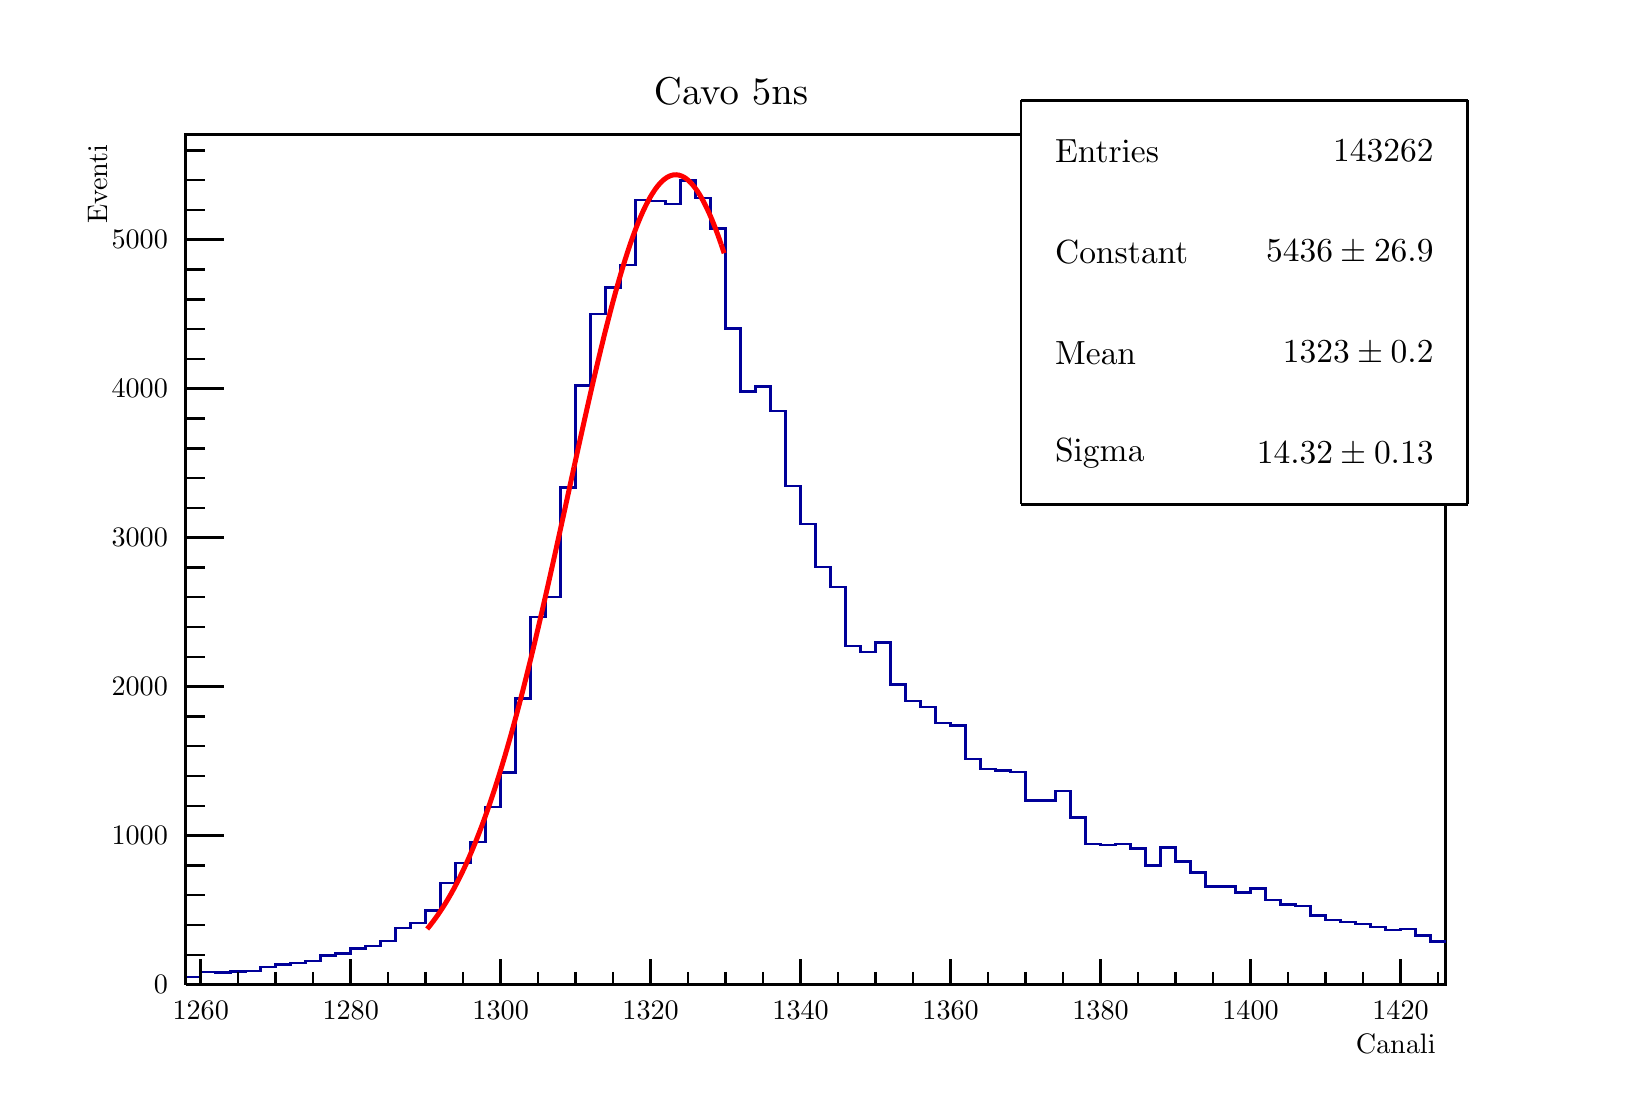
\begin{tikzpicture}
\pgfdeclareplotmark{cross} {
\pgfpathmoveto{\pgfpoint{-0.3\pgfplotmarksize}{\pgfplotmarksize}}
\pgfpathlineto{\pgfpoint{+0.3\pgfplotmarksize}{\pgfplotmarksize}}
\pgfpathlineto{\pgfpoint{+0.3\pgfplotmarksize}{0.3\pgfplotmarksize}}
\pgfpathlineto{\pgfpoint{+1\pgfplotmarksize}{0.3\pgfplotmarksize}}
\pgfpathlineto{\pgfpoint{+1\pgfplotmarksize}{-0.3\pgfplotmarksize}}
\pgfpathlineto{\pgfpoint{+0.3\pgfplotmarksize}{-0.3\pgfplotmarksize}}
\pgfpathlineto{\pgfpoint{+0.3\pgfplotmarksize}{-1.\pgfplotmarksize}}
\pgfpathlineto{\pgfpoint{-0.3\pgfplotmarksize}{-1.\pgfplotmarksize}}
\pgfpathlineto{\pgfpoint{-0.3\pgfplotmarksize}{-0.3\pgfplotmarksize}}
\pgfpathlineto{\pgfpoint{-1.\pgfplotmarksize}{-0.3\pgfplotmarksize}}
\pgfpathlineto{\pgfpoint{-1.\pgfplotmarksize}{0.3\pgfplotmarksize}}
\pgfpathlineto{\pgfpoint{-0.3\pgfplotmarksize}{0.3\pgfplotmarksize}}
\pgfpathclose
\pgfusepathqstroke
}
\pgfdeclareplotmark{cross*} {
\pgfpathmoveto{\pgfpoint{-0.3\pgfplotmarksize}{\pgfplotmarksize}}
\pgfpathlineto{\pgfpoint{+0.3\pgfplotmarksize}{\pgfplotmarksize}}
\pgfpathlineto{\pgfpoint{+0.3\pgfplotmarksize}{0.3\pgfplotmarksize}}
\pgfpathlineto{\pgfpoint{+1\pgfplotmarksize}{0.3\pgfplotmarksize}}
\pgfpathlineto{\pgfpoint{+1\pgfplotmarksize}{-0.3\pgfplotmarksize}}
\pgfpathlineto{\pgfpoint{+0.3\pgfplotmarksize}{-0.3\pgfplotmarksize}}
\pgfpathlineto{\pgfpoint{+0.3\pgfplotmarksize}{-1.\pgfplotmarksize}}
\pgfpathlineto{\pgfpoint{-0.3\pgfplotmarksize}{-1.\pgfplotmarksize}}
\pgfpathlineto{\pgfpoint{-0.3\pgfplotmarksize}{-0.3\pgfplotmarksize}}
\pgfpathlineto{\pgfpoint{-1.\pgfplotmarksize}{-0.3\pgfplotmarksize}}
\pgfpathlineto{\pgfpoint{-1.\pgfplotmarksize}{0.3\pgfplotmarksize}}
\pgfpathlineto{\pgfpoint{-0.3\pgfplotmarksize}{0.3\pgfplotmarksize}}
\pgfpathclose
\pgfusepathqfillstroke
}
\pgfdeclareplotmark{newstar} {
\pgfpathmoveto{\pgfqpoint{0pt}{\pgfplotmarksize}}
\pgfpathlineto{\pgfqpointpolar{44}{0.5\pgfplotmarksize}}
\pgfpathlineto{\pgfqpointpolar{18}{\pgfplotmarksize}}
\pgfpathlineto{\pgfqpointpolar{-20}{0.5\pgfplotmarksize}}
\pgfpathlineto{\pgfqpointpolar{-54}{\pgfplotmarksize}}
\pgfpathlineto{\pgfqpointpolar{-90}{0.5\pgfplotmarksize}}
\pgfpathlineto{\pgfqpointpolar{234}{\pgfplotmarksize}}
\pgfpathlineto{\pgfqpointpolar{198}{0.5\pgfplotmarksize}}
\pgfpathlineto{\pgfqpointpolar{162}{\pgfplotmarksize}}
\pgfpathlineto{\pgfqpointpolar{134}{0.5\pgfplotmarksize}}
\pgfpathclose
\pgfusepathqstroke
}
\pgfdeclareplotmark{newstar*} {
\pgfpathmoveto{\pgfqpoint{0pt}{\pgfplotmarksize}}
\pgfpathlineto{\pgfqpointpolar{44}{0.5\pgfplotmarksize}}
\pgfpathlineto{\pgfqpointpolar{18}{\pgfplotmarksize}}
\pgfpathlineto{\pgfqpointpolar{-20}{0.5\pgfplotmarksize}}
\pgfpathlineto{\pgfqpointpolar{-54}{\pgfplotmarksize}}
\pgfpathlineto{\pgfqpointpolar{-90}{0.5\pgfplotmarksize}}
\pgfpathlineto{\pgfqpointpolar{234}{\pgfplotmarksize}}
\pgfpathlineto{\pgfqpointpolar{198}{0.5\pgfplotmarksize}}
\pgfpathlineto{\pgfqpointpolar{162}{\pgfplotmarksize}}
\pgfpathlineto{\pgfqpointpolar{134}{0.5\pgfplotmarksize}}
\pgfpathclose
\pgfusepathqfillstroke
}
\definecolor{c}{rgb}{1,1,1};
\draw [color=c, fill=c] (0,0) rectangle (20,13.4957);
\draw [color=c, fill=c] (2,1.34957) rectangle (18,12.1461);
\definecolor{c}{rgb}{0,0,0};
\draw [c,line width=0.9] (2,1.34957) -- (2,12.1461) -- (18,12.1461) -- (18,1.34957) -- (2,1.34957);
\definecolor{c}{rgb}{1,1,1};
\draw [color=c, fill=c] (2,1.34957) rectangle (18,12.1461);
\definecolor{c}{rgb}{0,0,0};
\draw [c,line width=0.9] (2,1.34957) -- (2,12.1461) -- (18,12.1461) -- (18,1.34957) -- (2,1.34957);
\definecolor{c}{rgb}{0,0,0.6};
\draw [c,line width=0.9] (2,1.44418) -- (2.19048,1.44418) -- (2.19048,1.50662) -- (2.38095,1.50662) -- (2.38095,1.50472) -- (2.57143,1.50472) -- (2.57143,1.51418) -- (2.7619,1.51418) -- (2.7619,1.51986) -- (2.95238,1.51986) -- (2.95238,1.57095) --
 (3.14286,1.57095) -- (3.14286,1.60311) -- (3.33333,1.60311) -- (3.33333,1.62582) -- (3.52381,1.62582) -- (3.52381,1.64663) -- (3.71429,1.64663) -- (3.71429,1.72232) -- (3.90476,1.72232) -- (3.90476,1.74313) -- (4.09524,1.74313) -- (4.09524,1.81125)
 -- (4.28571,1.81125) -- (4.28571,1.83774) -- (4.47619,1.83774) -- (4.47619,1.90207) -- (4.66667,1.90207) -- (4.66667,2.06668) -- (4.85714,2.06668) -- (4.85714,2.13102) -- (5.04762,2.13102) -- (5.04762,2.28806) -- (5.2381,2.28806) -- (5.2381,2.6381)
 -- (5.42857,2.6381) -- (5.42857,2.89165) -- (5.61905,2.89165) -- (5.61905,3.16222) -- (5.80952,3.16222) -- (5.80952,3.60687) -- (6,3.60687) -- (6,4.04395) -- (6.19048,4.04395) -- (6.19048,4.98433) -- (6.38095,4.98433) -- (6.38095,6.01932) --
 (6.57143,6.01932) -- (6.57143,6.27286) -- (6.7619,6.27286) -- (6.7619,7.66167) -- (6.95238,7.66167) -- (6.95238,8.95588) -- (7.14286,8.95588) -- (7.14286,9.86788) -- (7.33333,9.86788) -- (7.33333,10.2047) -- (7.52381,10.2047) -- (7.52381,10.4866) --
 (7.71429,10.4866) -- (7.71429,11.3172) -- (7.90476,11.3172) -- (7.90476,11.304) -- (8.09524,11.304) -- (8.09524,11.2605) -- (8.28571,11.2605) -- (8.28571,11.5632) -- (8.47619,11.5632) -- (8.47619,11.3418) -- (8.66667,11.3418) -- (8.66667,10.954) --
 (8.85714,10.954) -- (8.85714,9.68246) -- (9.04762,9.68246) -- (9.04762,8.88398) -- (9.2381,8.88398) -- (9.2381,8.94832) -- (9.42857,8.94832) -- (9.42857,8.63422) -- (9.61905,8.63422) -- (9.61905,7.68438) -- (9.80952,7.68438) -- (9.80952,7.20189) --
 (10,7.20189) -- (10,6.65507) -- (10.1905,6.65507) -- (10.1905,6.39963) -- (10.381,6.39963) -- (10.381,5.65035) -- (10.5714,5.65035) -- (10.5714,5.57278) -- (10.7619,5.57278) -- (10.7619,5.69387) -- (10.9524,5.69387) -- (10.9524,5.1584) --
 (11.1429,5.1584) -- (11.1429,4.95216) -- (11.3333,4.95216) -- (11.3333,4.87459) -- (11.5238,4.87459) -- (11.5238,4.67024) -- (11.7143,4.67024) -- (11.7143,4.63807) -- (11.9048,4.63807) -- (11.9048,4.21613) -- (12.0952,4.21613) -- (12.0952,4.08557)
 -- (12.2857,4.08557) -- (12.2857,4.07044) -- (12.4762,4.07044) -- (12.4762,4.04962) -- (12.6667,4.04962) -- (12.6667,3.68634) -- (12.8571,3.68634) -- (12.8571,3.68823) -- (13.0476,3.68823) -- (13.0476,3.80932) -- (13.2381,3.80932) --
 (13.2381,3.47442) -- (13.4286,3.47442) -- (13.4286,3.13384) -- (13.619,3.13384) -- (13.619,3.12438) -- (13.8095,3.12438) -- (13.8095,3.13384) -- (14,3.13384) -- (14,3.07707) -- (14.1905,3.07707) -- (14.1905,2.86516) -- (14.381,2.86516) --
 (14.381,3.09032) -- (14.5714,3.09032) -- (14.5714,2.91057) -- (14.7619,2.91057) -- (14.7619,2.77055) -- (14.9524,2.77055) -- (14.9524,2.59458) -- (15.1429,2.59458) -- (15.1429,2.59648) -- (15.3333,2.59648) -- (15.3333,2.51701) -- (15.5238,2.51701)
 -- (15.5238,2.56809) -- (15.7143,2.56809) -- (15.7143,2.42429) -- (15.9048,2.42429) -- (15.9048,2.36942) -- (16.0952,2.36942) -- (16.0952,2.34482) -- (16.2857,2.34482) -- (16.2857,2.22941) -- (16.4762,2.22941) -- (16.4762,2.17264) --
 (16.6667,2.17264) -- (16.6667,2.14237) -- (16.8571,2.14237) -- (16.8571,2.11777) -- (17.0476,2.11777) -- (17.0476,2.07804) -- (17.2381,2.07804) -- (17.2381,2.04209) -- (17.4286,2.04209) -- (17.4286,2.05722) -- (17.619,2.05722) -- (17.619,1.97586) --
 (17.8095,1.97586) -- (17.8095,1.90018) -- (18,1.90018);
\definecolor{c}{rgb}{1,1,1};
\draw [color=c, fill=c] (12.6074,7.44986) rectangle (18.2808,12.5788);
\definecolor{c}{rgb}{0,0,0};
\draw [c,line width=0.9] (12.6074,7.44986) -- (18.2808,7.44986);
\draw [c,line width=0.9] (18.2808,7.44986) -- (18.2808,12.5788);
\draw [c,line width=0.9] (18.2808,12.5788) -- (12.6074,12.5788);
\draw [c,line width=0.9] (12.6074,12.5788) -- (12.6074,7.44986);
\draw [anchor= west] (12.8911,11.9377) node[scale=1.20912, color=c, rotate=0]{Entries };
\draw [anchor= east] (17.9971,11.9377) node[scale=1.20912, color=c, rotate=0]{ 143262};
\draw [anchor= west] (12.8911,10.6554) node[scale=1.20912, color=c, rotate=0]{Constant };
\draw [anchor= east] (17.9971,10.6554) node[scale=1.20912, color=c, rotate=0]{$  5436 \pm 26.9$};
\draw [anchor= west] (12.8911,9.37321) node[scale=1.20912, color=c, rotate=0]{Mean     };
\draw [anchor= east] (17.9971,9.37321) node[scale=1.20912, color=c, rotate=0]{$  1323 \pm 0.2$};
\draw [anchor= west] (12.8911,8.09097) node[scale=1.20912, color=c, rotate=0]{Sigma    };
\draw [anchor= east] (17.9971,8.09097) node[scale=1.20912, color=c, rotate=0]{$ 14.32 \pm 0.13$};
\definecolor{c}{rgb}{1,0,0};
\draw [c,line width=1.8] (5.06667,2.05651) -- (5.10476,2.10343) -- (5.14286,2.15283) -- (5.18095,2.2048) -- (5.21905,2.25943) -- (5.25714,2.31679) -- (5.29524,2.37696) -- (5.33333,2.44002) -- (5.37143,2.50605) -- (5.40952,2.57513) --
 (5.44762,2.64732) -- (5.48571,2.72268) -- (5.52381,2.80129) -- (5.5619,2.88321) -- (5.6,2.96848) -- (5.6381,3.05716) -- (5.67619,3.14929) -- (5.71429,3.24491) -- (5.75238,3.34406) -- (5.79048,3.44675) -- (5.82857,3.55302) -- (5.86667,3.66286) --
 (5.90476,3.77628) -- (5.94286,3.89328) -- (5.98095,4.01384) -- (6.01905,4.13794) -- (6.05714,4.26554) -- (6.09524,4.3966) -- (6.13333,4.53106) -- (6.17143,4.66887) -- (6.20952,4.80995) -- (6.24762,4.95421) -- (6.28571,5.10156) -- (6.32381,5.25188)
 -- (6.36191,5.40505) -- (6.4,5.56096) -- (6.4381,5.71944) -- (6.47619,5.88035) -- (6.51429,6.04352) -- (6.55238,6.20878) -- (6.59048,6.37593) -- (6.62857,6.54477) -- (6.66667,6.71509) -- (6.70476,6.88668) -- (6.74286,7.0593) -- (6.78095,7.2327) --
 (6.81905,7.40664) -- (6.85714,7.58086) -- (6.89524,7.75509) -- (6.93333,7.92906);
\draw [c,line width=1.8] (6.93333,7.92906) -- (6.97143,8.10247) -- (7.00952,8.27506) -- (7.04762,8.44651) -- (7.08571,8.61653) -- (7.12381,8.78482) -- (7.1619,8.95108) -- (7.2,9.11499) -- (7.2381,9.27625) -- (7.27619,9.43454) -- (7.31429,9.58956) --
 (7.35238,9.741) -- (7.39048,9.88856) -- (7.42857,10.0319) -- (7.46667,10.1708) -- (7.50476,10.305) -- (7.54286,10.434) -- (7.58095,10.5578) -- (7.61905,10.6759) -- (7.65714,10.7882) -- (7.69524,10.8944) -- (7.73333,10.9943) -- (7.77143,11.0876) --
 (7.80952,11.1741) -- (7.84762,11.2537) -- (7.88571,11.3261) -- (7.92381,11.3913) -- (7.96191,11.4489) -- (8,11.499) -- (8.0381,11.5413) -- (8.07619,11.5759) -- (8.11429,11.6026) -- (8.15238,11.6213) -- (8.19048,11.632) -- (8.22857,11.6347) --
 (8.26667,11.6294) -- (8.30476,11.6161) -- (8.34286,11.5948) -- (8.38095,11.5655) -- (8.41905,11.5284) -- (8.45714,11.4835) -- (8.49524,11.431) -- (8.53333,11.3709) -- (8.57143,11.3033) -- (8.60952,11.2286) -- (8.64762,11.1467) -- (8.68571,11.0579)
 -- (8.72381,10.9625) -- (8.7619,10.8605) -- (8.8,10.7523);
\draw [c,line width=1.8] (8.8,10.7523) -- (8.8381,10.6381);
\definecolor{c}{rgb}{0,0,0};
\draw [c,line width=0.9] (2,1.34957) -- (18,1.34957);
\draw [anchor= east] (18,0.593811) node[scale=1.01821, color=c, rotate=0]{Canali};
\draw [c,line width=0.9] (2.19048,1.67347) -- (2.19048,1.34957);
\draw [c,line width=0.9] (2.66667,1.51152) -- (2.66667,1.34957);
\draw [c,line width=0.9] (3.14286,1.51152) -- (3.14286,1.34957);
\draw [c,line width=0.9] (3.61905,1.51152) -- (3.61905,1.34957);
\draw [c,line width=0.9] (4.09524,1.67347) -- (4.09524,1.34957);
\draw [c,line width=0.9] (4.57143,1.51152) -- (4.57143,1.34957);
\draw [c,line width=0.9] (5.04762,1.51152) -- (5.04762,1.34957);
\draw [c,line width=0.9] (5.52381,1.51152) -- (5.52381,1.34957);
\draw [c,line width=0.9] (6,1.67347) -- (6,1.34957);
\draw [c,line width=0.9] (6.47619,1.51152) -- (6.47619,1.34957);
\draw [c,line width=0.9] (6.95238,1.51152) -- (6.95238,1.34957);
\draw [c,line width=0.9] (7.42857,1.51152) -- (7.42857,1.34957);
\draw [c,line width=0.9] (7.90476,1.67347) -- (7.90476,1.34957);
\draw [c,line width=0.9] (8.38095,1.51152) -- (8.38095,1.34957);
\draw [c,line width=0.9] (8.85714,1.51152) -- (8.85714,1.34957);
\draw [c,line width=0.9] (9.33333,1.51152) -- (9.33333,1.34957);
\draw [c,line width=0.9] (9.80952,1.67347) -- (9.80952,1.34957);
\draw [c,line width=0.9] (10.2857,1.51152) -- (10.2857,1.34957);
\draw [c,line width=0.9] (10.7619,1.51152) -- (10.7619,1.34957);
\draw [c,line width=0.9] (11.2381,1.51152) -- (11.2381,1.34957);
\draw [c,line width=0.9] (11.7143,1.67347) -- (11.7143,1.34957);
\draw [c,line width=0.9] (12.1905,1.51152) -- (12.1905,1.34957);
\draw [c,line width=0.9] (12.6667,1.51152) -- (12.6667,1.34957);
\draw [c,line width=0.9] (13.1429,1.51152) -- (13.1429,1.34957);
\draw [c,line width=0.9] (13.619,1.67347) -- (13.619,1.34957);
\draw [c,line width=0.9] (14.0952,1.51152) -- (14.0952,1.34957);
\draw [c,line width=0.9] (14.5714,1.51152) -- (14.5714,1.34957);
\draw [c,line width=0.9] (15.0476,1.51152) -- (15.0476,1.34957);
\draw [c,line width=0.9] (15.5238,1.67347) -- (15.5238,1.34957);
\draw [c,line width=0.9] (16,1.51152) -- (16,1.34957);
\draw [c,line width=0.9] (16.4762,1.51152) -- (16.4762,1.34957);
\draw [c,line width=0.9] (16.9524,1.51152) -- (16.9524,1.34957);
\draw [c,line width=0.9] (17.4286,1.67347) -- (17.4286,1.34957);
\draw [c,line width=0.9] (2.19048,1.67347) -- (2.19048,1.34957);
\draw [c,line width=0.9] (17.4286,1.67347) -- (17.4286,1.34957);
\draw [c,line width=0.9] (17.9048,1.51152) -- (17.9048,1.34957);
\draw [anchor=base] (2.19048,0.904212) node[scale=1.01821, color=c, rotate=0]{1260};
\draw [anchor=base] (4.09524,0.904212) node[scale=1.01821, color=c, rotate=0]{1280};
\draw [anchor=base] (6,0.904212) node[scale=1.01821, color=c, rotate=0]{1300};
\draw [anchor=base] (7.90476,0.904212) node[scale=1.01821, color=c, rotate=0]{1320};
\draw [anchor=base] (9.80952,0.904212) node[scale=1.01821, color=c, rotate=0]{1340};
\draw [anchor=base] (11.7143,0.904212) node[scale=1.01821, color=c, rotate=0]{1360};
\draw [anchor=base] (13.619,0.904212) node[scale=1.01821, color=c, rotate=0]{1380};
\draw [anchor=base] (15.5238,0.904212) node[scale=1.01821, color=c, rotate=0]{1400};
\draw [anchor=base] (17.4286,0.904212) node[scale=1.01821, color=c, rotate=0]{1420};
\draw [c,line width=0.9] (2,1.34957) -- (2,12.1461);
\draw [anchor= east] (0.88,12.1461) node[scale=1.01821, color=c, rotate=90]{Eventi};
\draw [c,line width=0.9] (2.48,1.34957) -- (2,1.34957);
\draw [c,line width=0.9] (2.24,1.72799) -- (2,1.72799);
\draw [c,line width=0.9] (2.24,2.10642) -- (2,2.10642);
\draw [c,line width=0.9] (2.24,2.48484) -- (2,2.48484);
\draw [c,line width=0.9] (2.24,2.86326) -- (2,2.86326);
\draw [c,line width=0.9] (2.48,3.24169) -- (2,3.24169);
\draw [c,line width=0.9] (2.24,3.62011) -- (2,3.62011);
\draw [c,line width=0.9] (2.24,3.99854) -- (2,3.99854);
\draw [c,line width=0.9] (2.24,4.37696) -- (2,4.37696);
\draw [c,line width=0.9] (2.24,4.75538) -- (2,4.75538);
\draw [c,line width=0.9] (2.48,5.13381) -- (2,5.13381);
\draw [c,line width=0.9] (2.24,5.51223) -- (2,5.51223);
\draw [c,line width=0.9] (2.24,5.89065) -- (2,5.89065);
\draw [c,line width=0.9] (2.24,6.26908) -- (2,6.26908);
\draw [c,line width=0.9] (2.24,6.6475) -- (2,6.6475);
\draw [c,line width=0.9] (2.48,7.02592) -- (2,7.02592);
\draw [c,line width=0.9] (2.24,7.40435) -- (2,7.40435);
\draw [c,line width=0.9] (2.24,7.78277) -- (2,7.78277);
\draw [c,line width=0.9] (2.24,8.16119) -- (2,8.16119);
\draw [c,line width=0.9] (2.24,8.53962) -- (2,8.53962);
\draw [c,line width=0.9] (2.48,8.91804) -- (2,8.91804);
\draw [c,line width=0.9] (2.24,9.29646) -- (2,9.29646);
\draw [c,line width=0.9] (2.24,9.67489) -- (2,9.67489);
\draw [c,line width=0.9] (2.24,10.0533) -- (2,10.0533);
\draw [c,line width=0.9] (2.24,10.4317) -- (2,10.4317);
\draw [c,line width=0.9] (2.48,10.8102) -- (2,10.8102);
\draw [c,line width=0.9] (2.48,10.8102) -- (2,10.8102);
\draw [c,line width=0.9] (2.24,11.1886) -- (2,11.1886);
\draw [c,line width=0.9] (2.24,11.567) -- (2,11.567);
\draw [c,line width=0.9] (2.24,11.9454) -- (2,11.9454);
\draw [anchor= east] (1.9,1.34957) node[scale=1.01821, color=c, rotate=0]{0};
\draw [anchor= east] (1.9,3.24169) node[scale=1.01821, color=c, rotate=0]{1000};
\draw [anchor= east] (1.9,5.13381) node[scale=1.01821, color=c, rotate=0]{2000};
\draw [anchor= east] (1.9,7.02592) node[scale=1.01821, color=c, rotate=0]{3000};
\draw [anchor= east] (1.9,8.91804) node[scale=1.01821, color=c, rotate=0]{4000};
\draw [anchor= east] (1.9,10.8102) node[scale=1.01821, color=c, rotate=0]{5000};
\definecolor{c}{rgb}{1,1,1};
\draw [color=c, fill=c] (12.6074,7.44986) rectangle (18.2808,12.5788);
\definecolor{c}{rgb}{0,0,0};
\draw [c,line width=0.9] (12.6074,7.44986) -- (18.2808,7.44986);
\draw [c,line width=0.9] (18.2808,7.44986) -- (18.2808,12.5788);
\draw [c,line width=0.9] (18.2808,12.5788) -- (12.6074,12.5788);
\draw [c,line width=0.9] (12.6074,12.5788) -- (12.6074,7.44986);
\draw [anchor= west] (12.8911,11.9377) node[scale=1.20912, color=c, rotate=0]{Entries };
\draw [anchor= east] (17.9971,11.9377) node[scale=1.20912, color=c, rotate=0]{ 143262};
\draw [anchor= west] (12.8911,10.6554) node[scale=1.20912, color=c, rotate=0]{Constant };
\draw [anchor= east] (17.9971,10.6554) node[scale=1.20912, color=c, rotate=0]{$  5436 \pm 26.9$};
\draw [anchor= west] (12.8911,9.37321) node[scale=1.20912, color=c, rotate=0]{Mean     };
\draw [anchor= east] (17.9971,9.37321) node[scale=1.20912, color=c, rotate=0]{$  1323 \pm 0.2$};
\draw [anchor= west] (12.8911,8.09097) node[scale=1.20912, color=c, rotate=0]{Sigma    };
\draw [anchor= east] (17.9971,8.09097) node[scale=1.20912, color=c, rotate=0]{$ 14.32 \pm 0.13$};
\draw (8.9255,12.6934) node[scale=1.40004, color=c, rotate=0]{Cavo 5ns};
\end{tikzpicture}

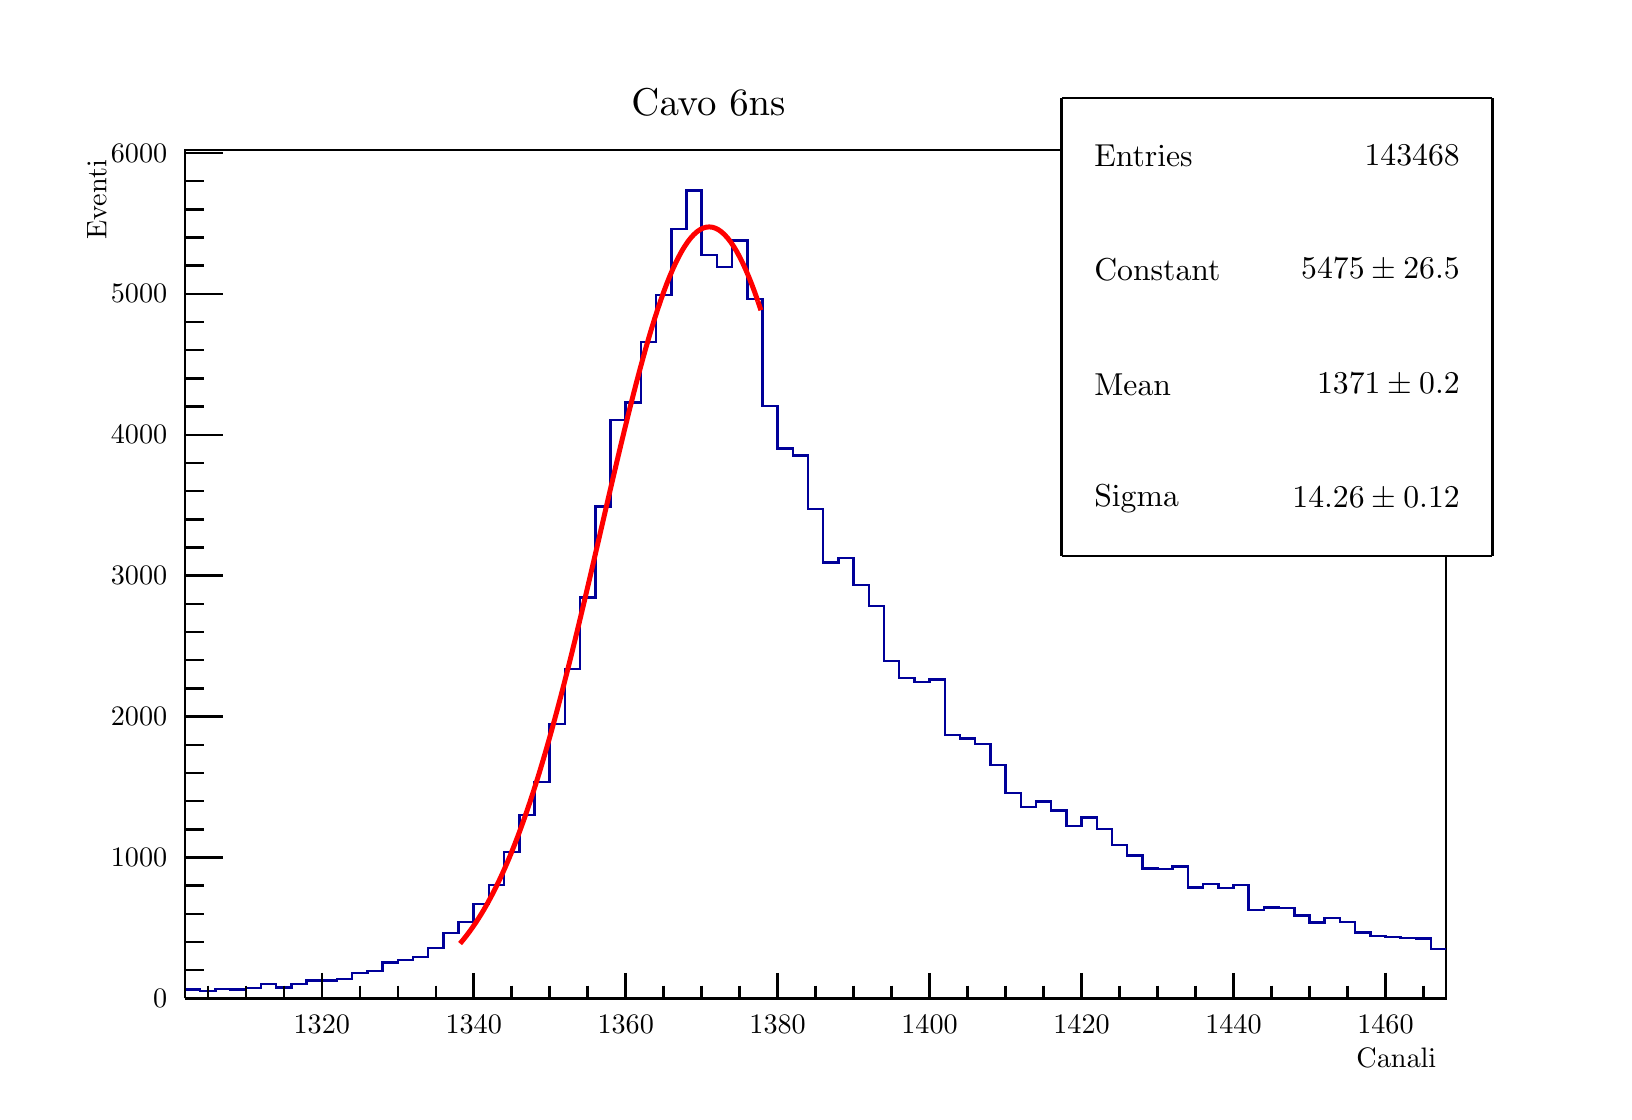
\begin{tikzpicture}
\pgfdeclareplotmark{cross} {
\pgfpathmoveto{\pgfpoint{-0.3\pgfplotmarksize}{\pgfplotmarksize}}
\pgfpathlineto{\pgfpoint{+0.3\pgfplotmarksize}{\pgfplotmarksize}}
\pgfpathlineto{\pgfpoint{+0.3\pgfplotmarksize}{0.3\pgfplotmarksize}}
\pgfpathlineto{\pgfpoint{+1\pgfplotmarksize}{0.3\pgfplotmarksize}}
\pgfpathlineto{\pgfpoint{+1\pgfplotmarksize}{-0.3\pgfplotmarksize}}
\pgfpathlineto{\pgfpoint{+0.3\pgfplotmarksize}{-0.3\pgfplotmarksize}}
\pgfpathlineto{\pgfpoint{+0.3\pgfplotmarksize}{-1.\pgfplotmarksize}}
\pgfpathlineto{\pgfpoint{-0.3\pgfplotmarksize}{-1.\pgfplotmarksize}}
\pgfpathlineto{\pgfpoint{-0.3\pgfplotmarksize}{-0.3\pgfplotmarksize}}
\pgfpathlineto{\pgfpoint{-1.\pgfplotmarksize}{-0.3\pgfplotmarksize}}
\pgfpathlineto{\pgfpoint{-1.\pgfplotmarksize}{0.3\pgfplotmarksize}}
\pgfpathlineto{\pgfpoint{-0.3\pgfplotmarksize}{0.3\pgfplotmarksize}}
\pgfpathclose
\pgfusepathqstroke
}
\pgfdeclareplotmark{cross*} {
\pgfpathmoveto{\pgfpoint{-0.3\pgfplotmarksize}{\pgfplotmarksize}}
\pgfpathlineto{\pgfpoint{+0.3\pgfplotmarksize}{\pgfplotmarksize}}
\pgfpathlineto{\pgfpoint{+0.3\pgfplotmarksize}{0.3\pgfplotmarksize}}
\pgfpathlineto{\pgfpoint{+1\pgfplotmarksize}{0.3\pgfplotmarksize}}
\pgfpathlineto{\pgfpoint{+1\pgfplotmarksize}{-0.3\pgfplotmarksize}}
\pgfpathlineto{\pgfpoint{+0.3\pgfplotmarksize}{-0.3\pgfplotmarksize}}
\pgfpathlineto{\pgfpoint{+0.3\pgfplotmarksize}{-1.\pgfplotmarksize}}
\pgfpathlineto{\pgfpoint{-0.3\pgfplotmarksize}{-1.\pgfplotmarksize}}
\pgfpathlineto{\pgfpoint{-0.3\pgfplotmarksize}{-0.3\pgfplotmarksize}}
\pgfpathlineto{\pgfpoint{-1.\pgfplotmarksize}{-0.3\pgfplotmarksize}}
\pgfpathlineto{\pgfpoint{-1.\pgfplotmarksize}{0.3\pgfplotmarksize}}
\pgfpathlineto{\pgfpoint{-0.3\pgfplotmarksize}{0.3\pgfplotmarksize}}
\pgfpathclose
\pgfusepathqfillstroke
}
\pgfdeclareplotmark{newstar} {
\pgfpathmoveto{\pgfqpoint{0pt}{\pgfplotmarksize}}
\pgfpathlineto{\pgfqpointpolar{44}{0.5\pgfplotmarksize}}
\pgfpathlineto{\pgfqpointpolar{18}{\pgfplotmarksize}}
\pgfpathlineto{\pgfqpointpolar{-20}{0.5\pgfplotmarksize}}
\pgfpathlineto{\pgfqpointpolar{-54}{\pgfplotmarksize}}
\pgfpathlineto{\pgfqpointpolar{-90}{0.5\pgfplotmarksize}}
\pgfpathlineto{\pgfqpointpolar{234}{\pgfplotmarksize}}
\pgfpathlineto{\pgfqpointpolar{198}{0.5\pgfplotmarksize}}
\pgfpathlineto{\pgfqpointpolar{162}{\pgfplotmarksize}}
\pgfpathlineto{\pgfqpointpolar{134}{0.5\pgfplotmarksize}}
\pgfpathclose
\pgfusepathqstroke
}
\pgfdeclareplotmark{newstar*} {
\pgfpathmoveto{\pgfqpoint{0pt}{\pgfplotmarksize}}
\pgfpathlineto{\pgfqpointpolar{44}{0.5\pgfplotmarksize}}
\pgfpathlineto{\pgfqpointpolar{18}{\pgfplotmarksize}}
\pgfpathlineto{\pgfqpointpolar{-20}{0.5\pgfplotmarksize}}
\pgfpathlineto{\pgfqpointpolar{-54}{\pgfplotmarksize}}
\pgfpathlineto{\pgfqpointpolar{-90}{0.5\pgfplotmarksize}}
\pgfpathlineto{\pgfqpointpolar{234}{\pgfplotmarksize}}
\pgfpathlineto{\pgfqpointpolar{198}{0.5\pgfplotmarksize}}
\pgfpathlineto{\pgfqpointpolar{162}{\pgfplotmarksize}}
\pgfpathlineto{\pgfqpointpolar{134}{0.5\pgfplotmarksize}}
\pgfpathclose
\pgfusepathqfillstroke
}
\definecolor{c}{rgb}{1,1,1};
\draw [color=c, fill=c] (0,0) rectangle (20,13.4957);
\draw [color=c, fill=c] (1.9914,1.17479) rectangle (18.0086,11.9484);
\definecolor{c}{rgb}{0,0,0};
\draw [c,line width=0.9] (1.9914,1.17479) -- (1.9914,11.9484) -- (18.0086,11.9484) -- (18.0086,1.17479) -- (1.9914,1.17479);
\definecolor{c}{rgb}{1,1,1};
\draw [color=c, fill=c] (1.9914,1.17479) rectangle (18.0086,11.9484);
\definecolor{c}{rgb}{0,0,0};
\draw [c,line width=0.9] (1.9914,1.17479) -- (1.9914,11.9484) -- (18.0086,11.9484) -- (18.0086,1.17479) -- (1.9914,1.17479);
\definecolor{c}{rgb}{0,0,0.6};
\draw [c,line width=0.9] (1.9914,1.28752) -- (2.18438,1.28752) -- (2.18438,1.27141) -- (2.37736,1.27141) -- (2.37736,1.29647) -- (2.57034,1.29647) -- (2.57034,1.28752) -- (2.76332,1.28752) -- (2.76332,1.30899) -- (2.9563,1.30899) -- (2.9563,1.3591)
 -- (3.14927,1.3591) -- (3.14927,1.31257) -- (3.34225,1.31257) -- (3.34225,1.3591) -- (3.53523,1.3591) -- (3.53523,1.40025) -- (3.72821,1.40025) -- (3.72821,1.40204) -- (3.92119,1.40204) -- (3.92119,1.42352) -- (4.11416,1.42352) -- (4.11416,1.49688)
 -- (4.30714,1.49688) -- (4.30714,1.52551) -- (4.50012,1.52551) -- (4.50012,1.6293) -- (4.6931,1.6293) -- (4.6931,1.65972) -- (4.88608,1.65972) -- (4.88608,1.70088) -- (5.07906,1.70088) -- (5.07906,1.81361) -- (5.27203,1.81361) -- (5.27203,2.00508)
 -- (5.46501,2.00508) -- (5.46501,2.14287) -- (5.65799,2.14287) -- (5.65799,2.37013) -- (5.85097,2.37013) -- (5.85097,2.61349) -- (6.04395,2.61349) -- (6.04395,3.03401) -- (6.23692,3.03401) -- (6.23692,3.50463) -- (6.4299,3.50463) -- (6.4299,3.92514)
 -- (6.62288,3.92514) -- (6.62288,4.6606) -- (6.81586,4.6606) -- (6.81586,5.36027) -- (7.00884,5.36027) -- (7.00884,6.26572) -- (7.20182,6.26572) -- (7.20182,7.41991) -- (7.39479,7.41991) -- (7.39479,8.52041) -- (7.58777,8.52041) -- (7.58777,8.74051)
 -- (7.78075,8.74051) -- (7.78075,9.51354) -- (7.97373,9.51354) -- (7.97373,10.1058) -- (8.16671,10.1058) -- (8.16671,10.9433) -- (8.35968,10.9433) -- (8.35968,11.4354) -- (8.55266,11.4354) -- (8.55266,10.614) -- (8.74564,10.614) -- (8.74564,10.4655)
 -- (8.93862,10.4655) -- (8.93862,10.7966) -- (9.1316,10.7966) -- (9.1316,10.0575) -- (9.32458,10.0575) -- (9.32458,8.69756) -- (9.51755,8.69756) -- (9.51755,8.15894) -- (9.71053,8.15894) -- (9.71053,8.06947) -- (9.90351,8.06947) -- (9.90351,7.39127)
 -- (10.0965,7.39127) -- (10.0965,6.70771) -- (10.2895,6.70771) -- (10.2895,6.77034) -- (10.4824,6.77034) -- (10.4824,6.42677) -- (10.6754,6.42677) -- (10.6754,6.15478) -- (10.8684,6.15478) -- (10.8684,5.4569) -- (11.0614,5.4569) -- (11.0614,5.24575)
 -- (11.2544,5.24575) -- (11.2544,5.19564) -- (11.4473,5.19564) -- (11.4473,5.22606) -- (11.6403,5.22606) -- (11.6403,4.51924) -- (11.8333,4.51924) -- (11.8333,4.47629) -- (12.0263,4.47629) -- (12.0263,4.40292) -- (12.2192,4.40292) --
 (12.2192,4.13988) -- (12.4122,4.13988) -- (12.4122,3.78557) -- (12.6052,3.78557) -- (12.6052,3.60841) -- (12.7982,3.60841) -- (12.7982,3.67462) -- (12.9912,3.67462) -- (12.9912,3.55831) -- (13.1841,3.55831) -- (13.1841,3.36505) -- (13.3771,3.36505)
 -- (13.3771,3.47063) -- (13.5701,3.47063) -- (13.5701,3.32747) -- (13.7631,3.32747) -- (13.7631,3.12348) -- (13.9561,3.12348) -- (13.9561,2.98748) -- (14.149,2.98748) -- (14.149,2.82643) -- (14.342,2.82643) -- (14.342,2.8157) -- (14.535,2.8157) --
 (14.535,2.8479) -- (14.728,2.8479) -- (14.728,2.58486) -- (14.9209,2.58486) -- (14.9209,2.6278) -- (15.1139,2.6278) -- (15.1139,2.57591) -- (15.3069,2.57591) -- (15.3069,2.61528) -- (15.4999,2.61528) -- (15.4999,2.30034) -- (15.6929,2.30034) --
 (15.6929,2.32897) -- (15.8858,2.32897) -- (15.8858,2.32181) -- (16.0788,2.32181) -- (16.0788,2.22876) -- (16.2718,2.22876) -- (16.2718,2.13929) -- (16.4648,2.13929) -- (16.4648,2.19834) -- (16.6577,2.19834) -- (16.6577,2.14466) -- (16.8507,2.14466)
 -- (16.8507,2.01224) -- (17.0437,2.01224) -- (17.0437,1.96571) -- (17.2367,1.96571) -- (17.2367,1.9514) -- (17.4297,1.9514) -- (17.4297,1.94424) -- (17.6226,1.94424) -- (17.6226,1.93529) -- (17.8156,1.93529) -- (17.8156,1.7993) -- (18.0086,1.7993);
\definecolor{c}{rgb}{1,1,1};
\draw [color=c, fill=c] (13.1232,6.79083) rectangle (18.596,12.6074);
\definecolor{c}{rgb}{0,0,0};
\draw [c,line width=0.9] (13.1232,6.79083) -- (18.596,6.79083);
\draw [c,line width=0.9] (18.596,6.79083) -- (18.596,12.6074);
\draw [c,line width=0.9] (18.596,12.6074) -- (13.1232,12.6074);
\draw [c,line width=0.9] (13.1232,12.6074) -- (13.1232,6.79083);
\draw [anchor= west] (13.3968,11.8804) node[scale=1.14549, color=c, rotate=0]{Entries };
\draw [anchor= east] (18.3223,11.8804) node[scale=1.14549, color=c, rotate=0]{ 143468};
\draw [anchor= west] (13.3968,10.4262) node[scale=1.14549, color=c, rotate=0]{Constant };
\draw [anchor= east] (18.3223,10.4262) node[scale=1.14549, color=c, rotate=0]{$  5475 \pm 26.5$};
\draw [anchor= west] (13.3968,8.97206) node[scale=1.14549, color=c, rotate=0]{Mean     };
\draw [anchor= east] (18.3223,8.97206) node[scale=1.14549, color=c, rotate=0]{$  1371 \pm 0.2$};
\draw [anchor= west] (13.3968,7.51791) node[scale=1.14549, color=c, rotate=0]{Sigma    };
\draw [anchor= east] (18.3223,7.51791) node[scale=1.14549, color=c, rotate=0]{$ 14.26 \pm 0.12$};
\definecolor{c}{rgb}{1,0,0};
\draw [c,line width=1.8] (5.48431,1.87119) -- (5.52291,1.91731) -- (5.5615,1.96586) -- (5.6001,2.01692) -- (5.63869,2.07057) -- (5.67729,2.12689) -- (5.71588,2.18596) -- (5.75448,2.24784) -- (5.79308,2.31262) -- (5.83167,2.38035) -- (5.87027,2.45112)
 -- (5.90886,2.52497) -- (5.94746,2.60197) -- (5.98605,2.68218) -- (6.02465,2.76564) -- (6.06324,2.85241) -- (6.10184,2.94251) -- (6.14044,3.03599) -- (6.17903,3.13286) -- (6.21763,3.23316) -- (6.25622,3.3369) -- (6.29482,3.44407) --
 (6.33341,3.55469) -- (6.37201,3.66873) -- (6.4106,3.78618) -- (6.4492,3.90701) -- (6.4878,4.03118) -- (6.52639,4.15864) -- (6.56499,4.28934) -- (6.60358,4.42321) -- (6.64218,4.56016) -- (6.68077,4.70011) -- (6.71937,4.84296) -- (6.75797,4.9886) --
 (6.79656,5.13689) -- (6.83516,5.28771) -- (6.87375,5.44092) -- (6.91235,5.59635) -- (6.95094,5.75384) -- (6.98954,5.9132) -- (7.02814,6.07426) -- (7.06673,6.2368) -- (7.10533,6.40062) -- (7.14392,6.56549) -- (7.18252,6.73119) -- (7.22111,6.89748) --
 (7.25971,7.06411) -- (7.29831,7.23082) -- (7.3369,7.39735) -- (7.3755,7.56342);
\draw [c,line width=1.8] (7.3755,7.56342) -- (7.41409,7.72877) -- (7.45269,7.89311) -- (7.49128,8.05615) -- (7.52988,8.2176) -- (7.56847,8.37717) -- (7.60707,8.53455) -- (7.64567,8.68946) -- (7.68426,8.84159) -- (7.72286,8.99064) -- (7.76145,9.13633)
 -- (7.80005,9.27835) -- (7.83864,9.41641) -- (7.87724,9.55023) -- (7.91584,9.67952) -- (7.95443,9.80401) -- (7.99303,9.92344) -- (8.03162,10.0375) -- (8.07022,10.1461) -- (8.10881,10.2488) -- (8.14741,10.3454) -- (8.186,10.4358) -- (8.2246,10.5198)
 -- (8.2632,10.597) -- (8.30179,10.6675) -- (8.34039,10.7309) -- (8.37898,10.7872) -- (8.41758,10.8362) -- (8.45617,10.8778) -- (8.49477,10.912) -- (8.53337,10.9385) -- (8.57196,10.9575) -- (8.61056,10.9687) -- (8.64915,10.9723) -- (8.68775,10.9681)
 -- (8.72634,10.9563) -- (8.76494,10.9368) -- (8.80354,10.9096) -- (8.84213,10.8749) -- (8.88073,10.8327) -- (8.91932,10.7831) -- (8.95792,10.7263) -- (8.99651,10.6623) -- (9.03511,10.5913) -- (9.0737,10.5135) -- (9.1123,10.4291) -- (9.1509,10.3382)
 -- (9.18949,10.2411) -- (9.22809,10.1379) -- (9.26668,10.0289);
\draw [c,line width=1.8] (9.26668,10.0289) -- (9.30528,9.91441);
\definecolor{c}{rgb}{0,0,0};
\draw [c,line width=0.9] (1.9914,1.17479) -- (18.0086,1.17479);
\draw [anchor= east] (18.0086,0.419026) node[scale=1.01821, color=c, rotate=0]{Canali};
\draw [c,line width=0.9] (3.72821,1.49903) -- (3.72821,1.17479);
\draw [c,line width=0.9] (4.21065,1.33691) -- (4.21065,1.17479);
\draw [c,line width=0.9] (4.6931,1.33691) -- (4.6931,1.17479);
\draw [c,line width=0.9] (5.17554,1.33691) -- (5.17554,1.17479);
\draw [c,line width=0.9] (5.65799,1.49903) -- (5.65799,1.17479);
\draw [c,line width=0.9] (6.14044,1.33691) -- (6.14044,1.17479);
\draw [c,line width=0.9] (6.62288,1.33691) -- (6.62288,1.17479);
\draw [c,line width=0.9] (7.10533,1.33691) -- (7.10533,1.17479);
\draw [c,line width=0.9] (7.58777,1.49903) -- (7.58777,1.17479);
\draw [c,line width=0.9] (8.07022,1.33691) -- (8.07022,1.17479);
\draw [c,line width=0.9] (8.55266,1.33691) -- (8.55266,1.17479);
\draw [c,line width=0.9] (9.03511,1.33691) -- (9.03511,1.17479);
\draw [c,line width=0.9] (9.51755,1.49903) -- (9.51755,1.17479);
\draw [c,line width=0.9] (10,1.33691) -- (10,1.17479);
\draw [c,line width=0.9] (10.4824,1.33691) -- (10.4824,1.17479);
\draw [c,line width=0.9] (10.9649,1.33691) -- (10.9649,1.17479);
\draw [c,line width=0.9] (11.4473,1.49903) -- (11.4473,1.17479);
\draw [c,line width=0.9] (11.9298,1.33691) -- (11.9298,1.17479);
\draw [c,line width=0.9] (12.4122,1.33691) -- (12.4122,1.17479);
\draw [c,line width=0.9] (12.8947,1.33691) -- (12.8947,1.17479);
\draw [c,line width=0.9] (13.3771,1.49903) -- (13.3771,1.17479);
\draw [c,line width=0.9] (13.8596,1.33691) -- (13.8596,1.17479);
\draw [c,line width=0.9] (14.342,1.33691) -- (14.342,1.17479);
\draw [c,line width=0.9] (14.8245,1.33691) -- (14.8245,1.17479);
\draw [c,line width=0.9] (15.3069,1.49903) -- (15.3069,1.17479);
\draw [c,line width=0.9] (15.7893,1.33691) -- (15.7893,1.17479);
\draw [c,line width=0.9] (16.2718,1.33691) -- (16.2718,1.17479);
\draw [c,line width=0.9] (16.7542,1.33691) -- (16.7542,1.17479);
\draw [c,line width=0.9] (17.2367,1.49903) -- (17.2367,1.17479);
\draw [c,line width=0.9] (3.72821,1.49903) -- (3.72821,1.17479);
\draw [c,line width=0.9] (3.24576,1.33691) -- (3.24576,1.17479);
\draw [c,line width=0.9] (2.76332,1.33691) -- (2.76332,1.17479);
\draw [c,line width=0.9] (2.28087,1.33691) -- (2.28087,1.17479);
\draw [c,line width=0.9] (17.2367,1.49903) -- (17.2367,1.17479);
\draw [c,line width=0.9] (17.7191,1.33691) -- (17.7191,1.17479);
\draw [anchor=base] (3.72821,0.729427) node[scale=1.01821, color=c, rotate=0]{1320};
\draw [anchor=base] (5.65799,0.729427) node[scale=1.01821, color=c, rotate=0]{1340};
\draw [anchor=base] (7.58777,0.729427) node[scale=1.01821, color=c, rotate=0]{1360};
\draw [anchor=base] (9.51755,0.729427) node[scale=1.01821, color=c, rotate=0]{1380};
\draw [anchor=base] (11.4473,0.729427) node[scale=1.01821, color=c, rotate=0]{1400};
\draw [anchor=base] (13.3771,0.729427) node[scale=1.01821, color=c, rotate=0]{1420};
\draw [anchor=base] (15.3069,0.729427) node[scale=1.01821, color=c, rotate=0]{1440};
\draw [anchor=base] (17.2367,0.729427) node[scale=1.01821, color=c, rotate=0]{1460};
\draw [c,line width=0.9] (1.9914,1.17479) -- (1.9914,11.9484);
\draw [anchor= east] (0.871404,11.9484) node[scale=1.01821, color=c, rotate=90]{Eventi};
\draw [c,line width=0.9] (2.47038,1.17479) -- (1.9914,1.17479);
\draw [c,line width=0.9] (2.23089,1.53267) -- (1.9914,1.53267);
\draw [c,line width=0.9] (2.23089,1.89056) -- (1.9914,1.89056);
\draw [c,line width=0.9] (2.23089,2.24844) -- (1.9914,2.24844);
\draw [c,line width=0.9] (2.23089,2.60633) -- (1.9914,2.60633);
\draw [c,line width=0.9] (2.47038,2.96422) -- (1.9914,2.96422);
\draw [c,line width=0.9] (2.23089,3.3221) -- (1.9914,3.3221);
\draw [c,line width=0.9] (2.23089,3.67999) -- (1.9914,3.67999);
\draw [c,line width=0.9] (2.23089,4.03788) -- (1.9914,4.03788);
\draw [c,line width=0.9] (2.23089,4.39576) -- (1.9914,4.39576);
\draw [c,line width=0.9] (2.47038,4.75365) -- (1.9914,4.75365);
\draw [c,line width=0.9] (2.23089,5.11154) -- (1.9914,5.11154);
\draw [c,line width=0.9] (2.23089,5.46942) -- (1.9914,5.46942);
\draw [c,line width=0.9] (2.23089,5.82731) -- (1.9914,5.82731);
\draw [c,line width=0.9] (2.23089,6.1852) -- (1.9914,6.1852);
\draw [c,line width=0.9] (2.47038,6.54308) -- (1.9914,6.54308);
\draw [c,line width=0.9] (2.23089,6.90097) -- (1.9914,6.90097);
\draw [c,line width=0.9] (2.23089,7.25886) -- (1.9914,7.25886);
\draw [c,line width=0.9] (2.23089,7.61674) -- (1.9914,7.61674);
\draw [c,line width=0.9] (2.23089,7.97463) -- (1.9914,7.97463);
\draw [c,line width=0.9] (2.47038,8.33252) -- (1.9914,8.33252);
\draw [c,line width=0.9] (2.23089,8.6904) -- (1.9914,8.6904);
\draw [c,line width=0.9] (2.23089,9.04829) -- (1.9914,9.04829);
\draw [c,line width=0.9] (2.23089,9.40618) -- (1.9914,9.40618);
\draw [c,line width=0.9] (2.23089,9.76406) -- (1.9914,9.76406);
\draw [c,line width=0.9] (2.47038,10.1219) -- (1.9914,10.1219);
\draw [c,line width=0.9] (2.23089,10.4798) -- (1.9914,10.4798);
\draw [c,line width=0.9] (2.23089,10.8377) -- (1.9914,10.8377);
\draw [c,line width=0.9] (2.23089,11.1956) -- (1.9914,11.1956);
\draw [c,line width=0.9] (2.23089,11.5535) -- (1.9914,11.5535);
\draw [c,line width=0.9] (2.47038,11.9114) -- (1.9914,11.9114);
\draw [c,line width=0.9] (2.47038,11.9114) -- (1.9914,11.9114);
\draw [anchor= east] (1.8914,1.17479) node[scale=1.01821, color=c, rotate=0]{0};
\draw [anchor= east] (1.8914,2.96422) node[scale=1.01821, color=c, rotate=0]{1000};
\draw [anchor= east] (1.8914,4.75365) node[scale=1.01821, color=c, rotate=0]{2000};
\draw [anchor= east] (1.8914,6.54308) node[scale=1.01821, color=c, rotate=0]{3000};
\draw [anchor= east] (1.8914,8.33252) node[scale=1.01821, color=c, rotate=0]{4000};
\draw [anchor= east] (1.8914,10.1219) node[scale=1.01821, color=c, rotate=0]{5000};
\draw [anchor= east] (1.8914,11.9114) node[scale=1.01821, color=c, rotate=0]{6000};
\definecolor{c}{rgb}{1,1,1};
\draw [color=c, fill=c] (13.1232,6.79083) rectangle (18.596,12.6074);
\definecolor{c}{rgb}{0,0,0};
\draw [c,line width=0.9] (13.1232,6.79083) -- (18.596,6.79083);
\draw [c,line width=0.9] (18.596,6.79083) -- (18.596,12.6074);
\draw [c,line width=0.9] (18.596,12.6074) -- (13.1232,12.6074);
\draw [c,line width=0.9] (13.1232,12.6074) -- (13.1232,6.79083);
\draw [anchor= west] (13.3968,11.8804) node[scale=1.14549, color=c, rotate=0]{Entries };
\draw [anchor= east] (18.3223,11.8804) node[scale=1.14549, color=c, rotate=0]{ 143468};
\draw [anchor= west] (13.3968,10.4262) node[scale=1.14549, color=c, rotate=0]{Constant };
\draw [anchor= east] (18.3223,10.4262) node[scale=1.14549, color=c, rotate=0]{$  5475 \pm 26.5$};
\draw [anchor= west] (13.3968,8.97206) node[scale=1.14549, color=c, rotate=0]{Mean     };
\draw [anchor= east] (18.3223,8.97206) node[scale=1.14549, color=c, rotate=0]{$  1371 \pm 0.2$};
\draw [anchor= west] (13.3968,7.51791) node[scale=1.14549, color=c, rotate=0]{Sigma    };
\draw [anchor= east] (18.3223,7.51791) node[scale=1.14549, color=c, rotate=0]{$ 14.26 \pm 0.12$};
\draw (8.63897,12.5501) node[scale=1.40004, color=c, rotate=0]{Cavo 6ns};
\end{tikzpicture}

%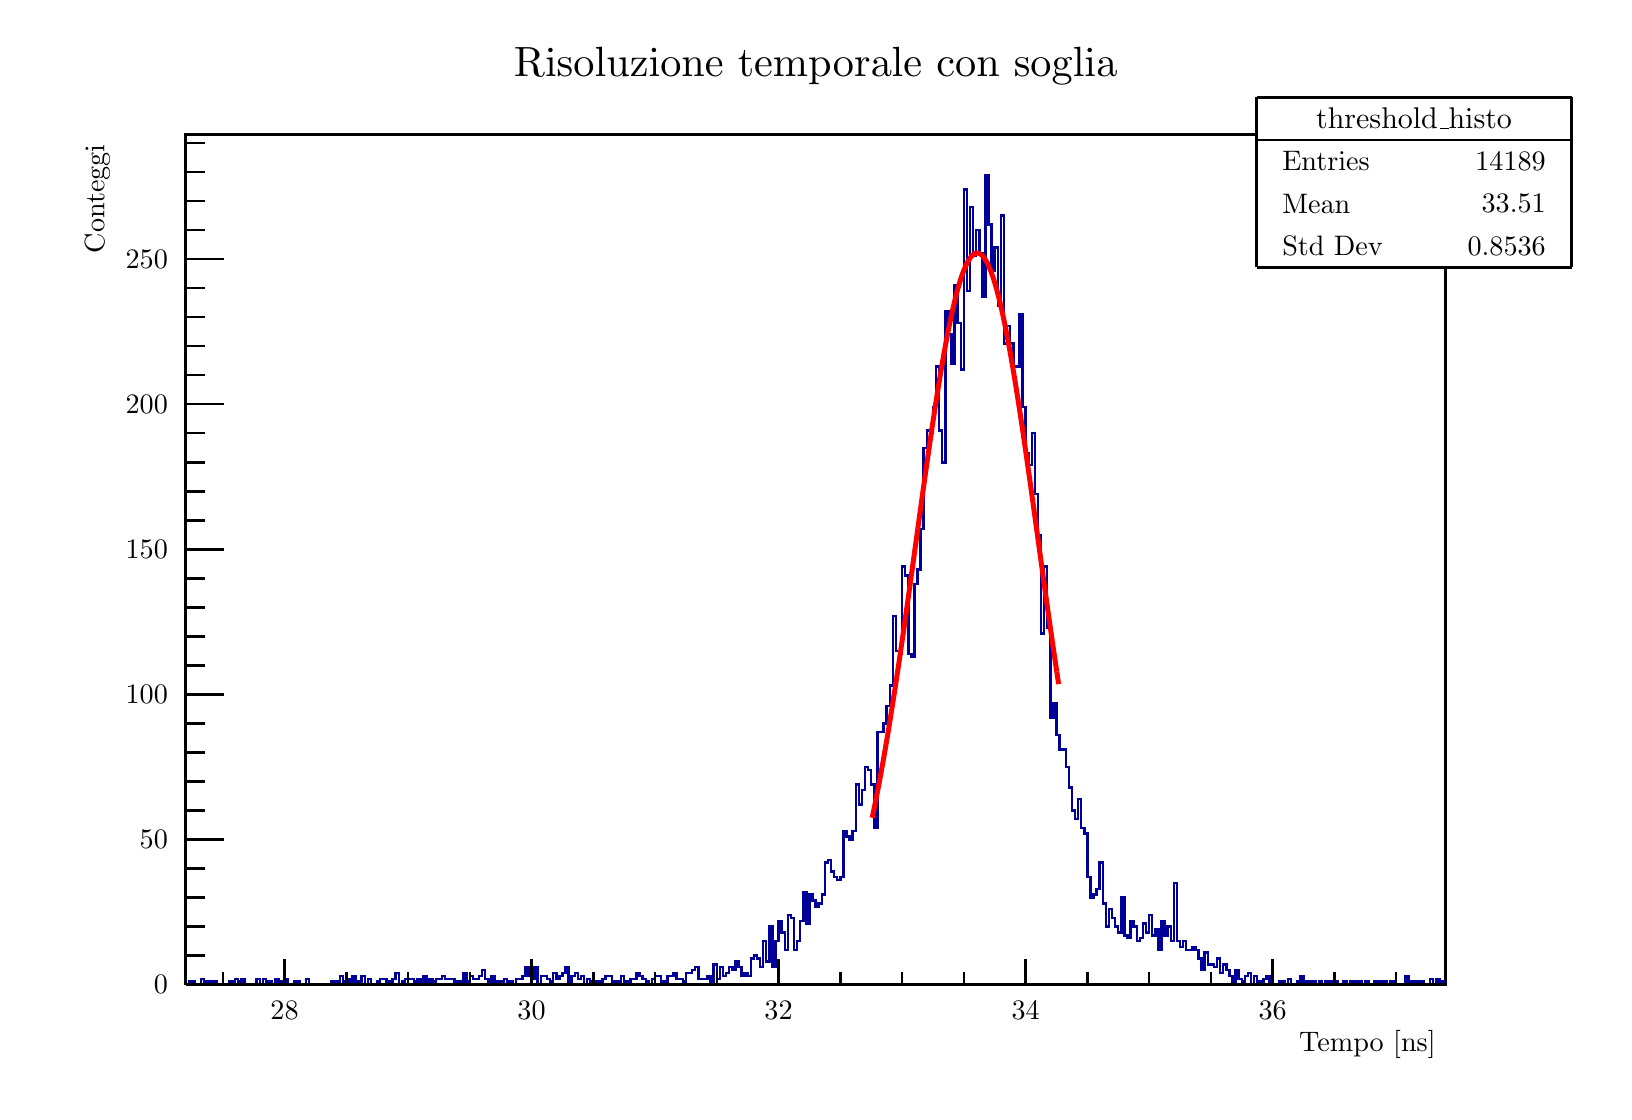
\begin{tikzpicture}
\pgfdeclareplotmark{cross} {
\pgfpathmoveto{\pgfpoint{-0.3\pgfplotmarksize}{\pgfplotmarksize}}
\pgfpathlineto{\pgfpoint{+0.3\pgfplotmarksize}{\pgfplotmarksize}}
\pgfpathlineto{\pgfpoint{+0.3\pgfplotmarksize}{0.3\pgfplotmarksize}}
\pgfpathlineto{\pgfpoint{+1\pgfplotmarksize}{0.3\pgfplotmarksize}}
\pgfpathlineto{\pgfpoint{+1\pgfplotmarksize}{-0.3\pgfplotmarksize}}
\pgfpathlineto{\pgfpoint{+0.3\pgfplotmarksize}{-0.3\pgfplotmarksize}}
\pgfpathlineto{\pgfpoint{+0.3\pgfplotmarksize}{-1.\pgfplotmarksize}}
\pgfpathlineto{\pgfpoint{-0.3\pgfplotmarksize}{-1.\pgfplotmarksize}}
\pgfpathlineto{\pgfpoint{-0.3\pgfplotmarksize}{-0.3\pgfplotmarksize}}
\pgfpathlineto{\pgfpoint{-1.\pgfplotmarksize}{-0.3\pgfplotmarksize}}
\pgfpathlineto{\pgfpoint{-1.\pgfplotmarksize}{0.3\pgfplotmarksize}}
\pgfpathlineto{\pgfpoint{-0.3\pgfplotmarksize}{0.3\pgfplotmarksize}}
\pgfpathclose
\pgfusepathqstroke
}
\pgfdeclareplotmark{cross*} {
\pgfpathmoveto{\pgfpoint{-0.3\pgfplotmarksize}{\pgfplotmarksize}}
\pgfpathlineto{\pgfpoint{+0.3\pgfplotmarksize}{\pgfplotmarksize}}
\pgfpathlineto{\pgfpoint{+0.3\pgfplotmarksize}{0.3\pgfplotmarksize}}
\pgfpathlineto{\pgfpoint{+1\pgfplotmarksize}{0.3\pgfplotmarksize}}
\pgfpathlineto{\pgfpoint{+1\pgfplotmarksize}{-0.3\pgfplotmarksize}}
\pgfpathlineto{\pgfpoint{+0.3\pgfplotmarksize}{-0.3\pgfplotmarksize}}
\pgfpathlineto{\pgfpoint{+0.3\pgfplotmarksize}{-1.\pgfplotmarksize}}
\pgfpathlineto{\pgfpoint{-0.3\pgfplotmarksize}{-1.\pgfplotmarksize}}
\pgfpathlineto{\pgfpoint{-0.3\pgfplotmarksize}{-0.3\pgfplotmarksize}}
\pgfpathlineto{\pgfpoint{-1.\pgfplotmarksize}{-0.3\pgfplotmarksize}}
\pgfpathlineto{\pgfpoint{-1.\pgfplotmarksize}{0.3\pgfplotmarksize}}
\pgfpathlineto{\pgfpoint{-0.3\pgfplotmarksize}{0.3\pgfplotmarksize}}
\pgfpathclose
\pgfusepathqfillstroke
}
\pgfdeclareplotmark{newstar} {
\pgfpathmoveto{\pgfqpoint{0pt}{\pgfplotmarksize}}
\pgfpathlineto{\pgfqpointpolar{44}{0.5\pgfplotmarksize}}
\pgfpathlineto{\pgfqpointpolar{18}{\pgfplotmarksize}}
\pgfpathlineto{\pgfqpointpolar{-20}{0.5\pgfplotmarksize}}
\pgfpathlineto{\pgfqpointpolar{-54}{\pgfplotmarksize}}
\pgfpathlineto{\pgfqpointpolar{-90}{0.5\pgfplotmarksize}}
\pgfpathlineto{\pgfqpointpolar{234}{\pgfplotmarksize}}
\pgfpathlineto{\pgfqpointpolar{198}{0.5\pgfplotmarksize}}
\pgfpathlineto{\pgfqpointpolar{162}{\pgfplotmarksize}}
\pgfpathlineto{\pgfqpointpolar{134}{0.5\pgfplotmarksize}}
\pgfpathclose
\pgfusepathqstroke
}
\pgfdeclareplotmark{newstar*} {
\pgfpathmoveto{\pgfqpoint{0pt}{\pgfplotmarksize}}
\pgfpathlineto{\pgfqpointpolar{44}{0.5\pgfplotmarksize}}
\pgfpathlineto{\pgfqpointpolar{18}{\pgfplotmarksize}}
\pgfpathlineto{\pgfqpointpolar{-20}{0.5\pgfplotmarksize}}
\pgfpathlineto{\pgfqpointpolar{-54}{\pgfplotmarksize}}
\pgfpathlineto{\pgfqpointpolar{-90}{0.5\pgfplotmarksize}}
\pgfpathlineto{\pgfqpointpolar{234}{\pgfplotmarksize}}
\pgfpathlineto{\pgfqpointpolar{198}{0.5\pgfplotmarksize}}
\pgfpathlineto{\pgfqpointpolar{162}{\pgfplotmarksize}}
\pgfpathlineto{\pgfqpointpolar{134}{0.5\pgfplotmarksize}}
\pgfpathclose
\pgfusepathqfillstroke
}
\definecolor{c}{rgb}{1,1,1};
\draw [color=c, fill=c] (0,0) rectangle (20,13.4957);
\draw [color=c, fill=c] (2,1.34957) rectangle (18,12.1461);
\definecolor{c}{rgb}{0,0,0};
\draw [c,line width=0.9] (2,1.34957) -- (2,12.1461) -- (18,12.1461) -- (18,1.34957) -- (2,1.34957);
\definecolor{c}{rgb}{1,1,1};
\draw [color=c, fill=c] (2,1.34957) rectangle (18,12.1461);
\definecolor{c}{rgb}{0,0,0};
\draw [c,line width=0.9] (2,1.34957) -- (2,12.1461) -- (18,12.1461) -- (18,1.34957) -- (2,1.34957);
\definecolor{c}{rgb}{0,0,0.6};
\draw [c,line width=0.9] (2,1.34957) -- (2.03922,1.34957) -- (2.03922,1.38642) -- (2.07843,1.38642) -- (2.07843,1.38642) -- (2.11765,1.38642) -- (2.11765,1.34957) -- (2.15686,1.34957) -- (2.15686,1.34957) -- (2.19608,1.34957) -- (2.19608,1.42328) --
 (2.23529,1.42328) -- (2.23529,1.38642) -- (2.27451,1.38642) -- (2.27451,1.38642) -- (2.31373,1.38642) -- (2.31373,1.34957) -- (2.35294,1.34957) -- (2.35294,1.38642) -- (2.39216,1.38642) -- (2.39216,1.34957) -- (2.43137,1.34957) -- (2.43137,1.34957)
 -- (2.47059,1.34957) -- (2.47059,1.34957) -- (2.5098,1.34957) -- (2.5098,1.34957) -- (2.54902,1.34957) -- (2.54902,1.38642) -- (2.58824,1.38642) -- (2.58824,1.38642) -- (2.62745,1.38642) -- (2.62745,1.42328) -- (2.66667,1.42328) -- (2.66667,1.38642)
 -- (2.70588,1.38642) -- (2.70588,1.42328) -- (2.7451,1.42328) -- (2.7451,1.34957) -- (2.78431,1.34957) -- (2.78431,1.34957) -- (2.82353,1.34957) -- (2.82353,1.34957) -- (2.86275,1.34957) -- (2.86275,1.34957) -- (2.90196,1.34957) -- (2.90196,1.42328)
 -- (2.94118,1.42328) -- (2.94118,1.34957) -- (2.98039,1.34957) -- (2.98039,1.42328) -- (3.01961,1.42328) -- (3.01961,1.38642) -- (3.05882,1.38642) -- (3.05882,1.38642) -- (3.09804,1.38642) -- (3.09804,1.34957) -- (3.13725,1.34957) --
 (3.13725,1.42328) -- (3.17647,1.42328) -- (3.17647,1.38642) -- (3.21569,1.38642) -- (3.21569,1.38642) -- (3.2549,1.38642) -- (3.2549,1.42328) -- (3.29412,1.42328) -- (3.29412,1.34957) -- (3.33333,1.34957) -- (3.33333,1.34957) -- (3.37255,1.34957) --
 (3.37255,1.38642) -- (3.41176,1.38642) -- (3.41176,1.38642) -- (3.45098,1.38642) -- (3.45098,1.34957) -- (3.4902,1.34957) -- (3.4902,1.34957) -- (3.52941,1.34957) -- (3.52941,1.42328) -- (3.56863,1.42328) -- (3.56863,1.34957) -- (3.60784,1.34957) --
 (3.60784,1.34957) -- (3.64706,1.34957) -- (3.64706,1.34957) -- (3.68627,1.34957) -- (3.68627,1.34957) -- (3.72549,1.34957) -- (3.72549,1.34957) -- (3.76471,1.34957) -- (3.76471,1.34957) -- (3.80392,1.34957) -- (3.80392,1.34957) -- (3.84314,1.34957)
 -- (3.84314,1.38642) -- (3.88235,1.38642) -- (3.88235,1.38642) -- (3.92157,1.38642) -- (3.92157,1.38642) -- (3.96078,1.38642) -- (3.96078,1.46013) -- (4,1.46013) -- (4,1.38642) -- (4.03922,1.38642) -- (4.03922,1.42328) -- (4.07843,1.42328) --
 (4.07843,1.38642) -- (4.11765,1.38642) -- (4.11765,1.46013) -- (4.15686,1.46013) -- (4.15686,1.38642) -- (4.19608,1.38642) -- (4.19608,1.38642) -- (4.23529,1.38642) -- (4.23529,1.46013) -- (4.27451,1.46013) -- (4.27451,1.34957) -- (4.31373,1.34957)
 -- (4.31373,1.42328) -- (4.35294,1.42328) -- (4.35294,1.34957) -- (4.39216,1.34957) -- (4.39216,1.34957) -- (4.43137,1.34957) -- (4.43137,1.38642) -- (4.47059,1.38642) -- (4.47059,1.42328) -- (4.5098,1.42328) -- (4.5098,1.42328) -- (4.54902,1.42328)
 -- (4.54902,1.38642) -- (4.58824,1.38642) -- (4.58824,1.34957) -- (4.62745,1.34957) -- (4.62745,1.42328) -- (4.66667,1.42328) -- (4.66667,1.49699) -- (4.70588,1.49699) -- (4.70588,1.34957) -- (4.7451,1.34957) -- (4.7451,1.38642) -- (4.78431,1.38642)
 -- (4.78431,1.42328) -- (4.82353,1.42328) -- (4.82353,1.42328) -- (4.86275,1.42328) -- (4.86275,1.42328) -- (4.90196,1.42328) -- (4.90196,1.38642) -- (4.94118,1.38642) -- (4.94118,1.42328) -- (4.98039,1.42328) -- (4.98039,1.38642) --
 (5.01961,1.38642) -- (5.01961,1.46013) -- (5.05882,1.46013) -- (5.05882,1.34957) -- (5.09804,1.34957) -- (5.09804,1.42328) -- (5.13726,1.42328) -- (5.13726,1.38642) -- (5.17647,1.38642) -- (5.17647,1.42328) -- (5.21569,1.42328) -- (5.21569,1.42328)
 -- (5.2549,1.42328) -- (5.2549,1.46013) -- (5.29412,1.46013) -- (5.29412,1.42328) -- (5.33333,1.42328) -- (5.33333,1.42328) -- (5.37255,1.42328) -- (5.37255,1.42328) -- (5.41176,1.42328) -- (5.41176,1.38642) -- (5.45098,1.38642) -- (5.45098,1.38642)
 -- (5.4902,1.38642) -- (5.4902,1.38642) -- (5.52941,1.38642) -- (5.52941,1.49699) -- (5.56863,1.49699) -- (5.56863,1.38642) -- (5.60784,1.38642) -- (5.60784,1.46013) -- (5.64706,1.46013) -- (5.64706,1.42328) -- (5.68627,1.42328) -- (5.68627,1.42328)
 -- (5.72549,1.42328) -- (5.72549,1.46013) -- (5.76471,1.46013) -- (5.76471,1.53384) -- (5.80392,1.53384) -- (5.80392,1.42328) -- (5.84314,1.42328) -- (5.84314,1.38642) -- (5.88235,1.38642) -- (5.88235,1.46013) -- (5.92157,1.46013) --
 (5.92157,1.38642) -- (5.96078,1.38642) -- (5.96078,1.38642) -- (6,1.38642) -- (6,1.38642) -- (6.03922,1.38642) -- (6.03922,1.42328) -- (6.07843,1.42328) -- (6.07843,1.38642) -- (6.11765,1.38642) -- (6.11765,1.38642) -- (6.15686,1.38642) --
 (6.15686,1.34957) -- (6.19608,1.34957) -- (6.19608,1.42328) -- (6.23529,1.42328) -- (6.23529,1.42328) -- (6.27451,1.42328) -- (6.27451,1.46013) -- (6.31373,1.46013) -- (6.31373,1.5707) -- (6.35294,1.5707) -- (6.35294,1.46013) -- (6.39216,1.46013) --
 (6.39216,1.42328) -- (6.43137,1.42328) -- (6.43137,1.5707) -- (6.47059,1.5707) -- (6.47059,1.34957) -- (6.5098,1.34957) -- (6.5098,1.46013) -- (6.54902,1.46013) -- (6.54902,1.46013) -- (6.58824,1.46013) -- (6.58824,1.42328) -- (6.62745,1.42328) --
 (6.62745,1.38642) -- (6.66667,1.38642) -- (6.66667,1.49699) -- (6.70588,1.49699) -- (6.70588,1.42328) -- (6.7451,1.42328) -- (6.7451,1.46013) -- (6.78431,1.46013) -- (6.78431,1.49699) -- (6.82353,1.49699) -- (6.82353,1.5707) -- (6.86275,1.5707) --
 (6.86275,1.34957) -- (6.90196,1.34957) -- (6.90196,1.46013) -- (6.94118,1.46013) -- (6.94118,1.49699) -- (6.98039,1.49699) -- (6.98039,1.42328) -- (7.01961,1.42328) -- (7.01961,1.46013) -- (7.05882,1.46013) -- (7.05882,1.34957) -- (7.09804,1.34957)
 -- (7.09804,1.42328) -- (7.13725,1.42328) -- (7.13725,1.38642) -- (7.17647,1.38642) -- (7.17647,1.38642) -- (7.21569,1.38642) -- (7.21569,1.34957) -- (7.2549,1.34957) -- (7.2549,1.38642) -- (7.29412,1.38642) -- (7.29412,1.42328) -- (7.33333,1.42328)
 -- (7.33333,1.46013) -- (7.37255,1.46013) -- (7.37255,1.46013) -- (7.41176,1.46013) -- (7.41176,1.38642) -- (7.45098,1.38642) -- (7.45098,1.38642) -- (7.4902,1.38642) -- (7.4902,1.38642) -- (7.52941,1.38642) -- (7.52941,1.46013) -- (7.56863,1.46013)
 -- (7.56863,1.38642) -- (7.60784,1.38642) -- (7.60784,1.34957) -- (7.64706,1.34957) -- (7.64706,1.42328) -- (7.68627,1.42328) -- (7.68627,1.42328) -- (7.72549,1.42328) -- (7.72549,1.49699) -- (7.76471,1.49699) -- (7.76471,1.46013) --
 (7.80392,1.46013) -- (7.80392,1.42328) -- (7.84314,1.42328) -- (7.84314,1.38642) -- (7.88235,1.38642) -- (7.88235,1.34957) -- (7.92157,1.34957) -- (7.92157,1.42328) -- (7.96078,1.42328) -- (7.96078,1.46013) -- (8,1.46013) -- (8,1.46013) --
 (8.03922,1.46013) -- (8.03922,1.38642) -- (8.07843,1.38642) -- (8.07843,1.38642) -- (8.11765,1.38642) -- (8.11765,1.46013) -- (8.15686,1.46013) -- (8.15686,1.46013) -- (8.19608,1.46013) -- (8.19608,1.49699) -- (8.23529,1.49699) -- (8.23529,1.42328)
 -- (8.27451,1.42328) -- (8.27451,1.42328) -- (8.31373,1.42328) -- (8.31373,1.38642) -- (8.35294,1.38642) -- (8.35294,1.49699) -- (8.39216,1.49699) -- (8.39216,1.49699) -- (8.43137,1.49699) -- (8.43137,1.53384) -- (8.47059,1.53384) --
 (8.47059,1.5707) -- (8.5098,1.5707) -- (8.5098,1.42328) -- (8.54902,1.42328) -- (8.54902,1.42328) -- (8.58823,1.42328) -- (8.58823,1.42328) -- (8.62745,1.42328) -- (8.62745,1.46013) -- (8.66667,1.46013) -- (8.66667,1.38642) -- (8.70588,1.38642) --
 (8.70588,1.60755) -- (8.7451,1.60755) -- (8.7451,1.42328) -- (8.78431,1.42328) -- (8.78431,1.5707) -- (8.82353,1.5707) -- (8.82353,1.46013) -- (8.86275,1.46013) -- (8.86275,1.49699) -- (8.90196,1.49699) -- (8.90196,1.5707) -- (8.94118,1.5707) --
 (8.94118,1.53384) -- (8.98039,1.53384) -- (8.98039,1.64441) -- (9.01961,1.64441) -- (9.01961,1.5707) -- (9.05882,1.5707) -- (9.05882,1.46013) -- (9.09804,1.46013) -- (9.09804,1.49699) -- (9.13725,1.49699) -- (9.13725,1.46013) -- (9.17647,1.46013) --
 (9.17647,1.68126) -- (9.21569,1.68126) -- (9.21569,1.71812) -- (9.2549,1.71812) -- (9.2549,1.68126) -- (9.29412,1.68126) -- (9.29412,1.5707) -- (9.33333,1.5707) -- (9.33333,1.90239) -- (9.37255,1.90239) -- (9.37255,1.64441) -- (9.41177,1.64441) --
 (9.41177,2.08666) -- (9.45098,2.08666) -- (9.45098,1.5707) -- (9.4902,1.5707) -- (9.4902,1.90239) -- (9.52941,1.90239) -- (9.52941,2.16037) -- (9.56863,2.16037) -- (9.56863,2.01295) -- (9.60784,2.01295) -- (9.60784,1.79183) -- (9.64706,1.79183) --
 (9.64706,2.23408) -- (9.68627,2.23408) -- (9.68627,2.19723) -- (9.72549,2.19723) -- (9.72549,1.79183) -- (9.76471,1.79183) -- (9.76471,1.90239) -- (9.80392,1.90239) -- (9.80392,2.16037) -- (9.84314,2.16037) -- (9.84314,2.52892) -- (9.88235,2.52892)
 -- (9.88235,2.12352) -- (9.92157,2.12352) -- (9.92157,2.49206) -- (9.96078,2.49206) -- (9.96078,2.41835) -- (10,2.41835) -- (10,2.34465) -- (10.0392,2.34465) -- (10.0392,2.3815) -- (10.0784,2.3815) -- (10.0784,2.49206) -- (10.1176,2.49206) --
 (10.1176,2.89746) -- (10.1569,2.89746) -- (10.1569,2.93432) -- (10.1961,2.93432) -- (10.1961,2.7869) -- (10.2353,2.7869) -- (10.2353,2.71319) -- (10.2745,2.71319) -- (10.2745,2.67634) -- (10.3137,2.67634) -- (10.3137,2.71319) -- (10.3529,2.71319) --
 (10.3529,3.30287) -- (10.3922,3.30287) -- (10.3922,3.22916) -- (10.4314,3.22916) -- (10.4314,3.1923) -- (10.4706,3.1923) -- (10.4706,3.30287) -- (10.5098,3.30287) -- (10.5098,3.89254) -- (10.549,3.89254) -- (10.549,3.63456) -- (10.5882,3.63456) --
 (10.5882,3.81883) -- (10.6275,3.81883) -- (10.6275,4.11367) -- (10.6667,4.11367) -- (10.6667,4.07681) -- (10.7059,4.07681) -- (10.7059,3.89254) -- (10.7451,3.89254) -- (10.7451,3.33972) -- (10.7843,3.33972) -- (10.7843,4.55592) -- (10.8235,4.55592)
 -- (10.8235,4.55592) -- (10.8627,4.55592) -- (10.8627,4.66649) -- (10.902,4.66649) -- (10.902,4.88761) -- (10.9412,4.88761) -- (10.9412,5.1456) -- (10.9804,5.1456) -- (10.9804,6.03011) -- (11.0196,6.03011) -- (11.0196,5.58785) -- (11.0588,5.58785)
 -- (11.0588,5.551) -- (11.098,5.551) -- (11.098,6.65664) -- (11.1373,6.65664) -- (11.1373,6.54607) -- (11.1765,6.54607) -- (11.1765,5.551) -- (11.2157,5.551) -- (11.2157,5.51414) -- (11.2549,5.51414) -- (11.2549,6.43551) -- (11.2941,6.43551) --
 (11.2941,6.61978) -- (11.3333,6.61978) -- (11.3333,7.13575) -- (11.3725,7.13575) -- (11.3725,8.16768) -- (11.4118,8.16768) -- (11.4118,8.3888) -- (11.451,8.3888) -- (11.451,8.35195) -- (11.4902,8.35195) -- (11.4902,8.68364) -- (11.5294,8.68364) --
 (11.5294,9.1996) -- (11.5686,9.1996) -- (11.5686,8.3888) -- (11.6078,8.3888) -- (11.6078,7.9834) -- (11.6471,7.9834) -- (11.6471,9.89984) -- (11.6863,9.89984) -- (11.6863,9.60501) -- (11.7255,9.60501) -- (11.7255,9.23646) -- (11.7647,9.23646) --
 (11.7647,10.2315) -- (11.8039,10.2315) -- (11.8039,9.75242) -- (11.8431,9.75242) -- (11.8431,9.16275) -- (11.8824,9.16275) -- (11.8824,11.4477) -- (11.9216,11.4477) -- (11.9216,10.1578) -- (11.9608,10.1578) -- (11.9608,11.2266) -- (12,11.2266) --
 (12,10.6001) -- (12.0392,10.6001) -- (12.0392,10.9318) -- (12.0784,10.9318) -- (12.0784,10.6369) -- (12.1176,10.6369) -- (12.1176,10.0841) -- (12.1569,10.0841) -- (12.1569,11.632) -- (12.1961,11.632) -- (12.1961,11.0055) -- (12.2353,11.0055) --
 (12.2353,10.4158) -- (12.2745,10.4158) -- (12.2745,10.7106) -- (12.3137,10.7106) -- (12.3137,9.97355) -- (12.3529,9.97355) -- (12.3529,11.116) -- (12.3922,11.116) -- (12.3922,9.49444) -- (12.4314,9.49444) -- (12.4314,9.71557) -- (12.4706,9.71557) --
 (12.4706,9.49444) -- (12.5098,9.49444) -- (12.5098,9.1996) -- (12.549,9.1996) -- (12.549,9.1996) -- (12.5882,9.1996) -- (12.5882,9.86299) -- (12.6275,9.86299) -- (12.6275,8.68364) -- (12.6667,8.68364) -- (12.6667,8.09397) -- (12.7059,8.09397) --
 (12.7059,7.94655) -- (12.7451,7.94655) -- (12.7451,8.35195) -- (12.7843,8.35195) -- (12.7843,7.578) -- (12.8235,7.578) -- (12.8235,7.06204) -- (12.8627,7.06204) -- (12.8627,5.80898) -- (12.902,5.80898) -- (12.902,6.65664) -- (12.9412,6.65664) --
 (12.9412,5.88269) -- (12.9804,5.88269) -- (12.9804,4.7402) -- (13.0196,4.7402) -- (13.0196,4.92447) -- (13.0588,4.92447) -- (13.0588,4.51907) -- (13.098,4.51907) -- (13.098,4.33479) -- (13.1373,4.33479) -- (13.1373,4.33479) -- (13.1765,4.33479) --
 (13.1765,4.11367) -- (13.2157,4.11367) -- (13.2157,3.85568) -- (13.2549,3.85568) -- (13.2549,3.56085) -- (13.2941,3.56085) -- (13.2941,3.45028) -- (13.3333,3.45028) -- (13.3333,3.70827) -- (13.3725,3.70827) -- (13.3725,3.33972) -- (13.4118,3.33972)
 -- (13.4118,3.26601) -- (13.451,3.26601) -- (13.451,2.71319) -- (13.4902,2.71319) -- (13.4902,2.45521) -- (13.5294,2.45521) -- (13.5294,2.49206) -- (13.5686,2.49206) -- (13.5686,2.56577) -- (13.6078,2.56577) -- (13.6078,2.89746) -- (13.6471,2.89746)
 -- (13.6471,2.3815) -- (13.6863,2.3815) -- (13.6863,2.08666) -- (13.7255,2.08666) -- (13.7255,2.30779) -- (13.7647,2.30779) -- (13.7647,2.19723) -- (13.8039,2.19723) -- (13.8039,2.08666) -- (13.8431,2.08666) -- (13.8431,2.01295) -- (13.8824,2.01295)
 -- (13.8824,2.45521) -- (13.9216,2.45521) -- (13.9216,1.9761) -- (13.9608,1.9761) -- (13.9608,1.93924) -- (14,1.93924) -- (14,2.16037) -- (14.0392,2.16037) -- (14.0392,2.08666) -- (14.0784,2.08666) -- (14.0784,1.90239) -- (14.1176,1.90239) --
 (14.1176,1.93924) -- (14.1569,1.93924) -- (14.1569,2.12352) -- (14.1961,2.12352) -- (14.1961,2.01295) -- (14.2353,2.01295) -- (14.2353,2.23408) -- (14.2745,2.23408) -- (14.2745,1.9761) -- (14.3137,1.9761) -- (14.3137,2.04981) -- (14.3529,2.04981) --
 (14.3529,1.79183) -- (14.3922,1.79183) -- (14.3922,2.16037) -- (14.4314,2.16037) -- (14.4314,1.9761) -- (14.4706,1.9761) -- (14.4706,2.08666) -- (14.5098,2.08666) -- (14.5098,1.90239) -- (14.549,1.90239) -- (14.549,2.63948) -- (14.5882,2.63948) --
 (14.5882,1.90239) -- (14.6275,1.90239) -- (14.6275,1.82868) -- (14.6667,1.82868) -- (14.6667,1.90239) -- (14.7059,1.90239) -- (14.7059,1.79183) -- (14.7451,1.79183) -- (14.7451,1.79183) -- (14.7843,1.79183) -- (14.7843,1.82868) -- (14.8235,1.82868)
 -- (14.8235,1.79183) -- (14.8627,1.79183) -- (14.8627,1.68126) -- (14.902,1.68126) -- (14.902,1.53384) -- (14.9412,1.53384) -- (14.9412,1.75497) -- (14.9804,1.75497) -- (14.9804,1.60755) -- (15.0196,1.60755) -- (15.0196,1.60755) -- (15.0588,1.60755)
 -- (15.0588,1.5707) -- (15.098,1.5707) -- (15.098,1.68126) -- (15.1373,1.68126) -- (15.1373,1.49699) -- (15.1765,1.49699) -- (15.1765,1.60755) -- (15.2157,1.60755) -- (15.2157,1.53384) -- (15.2549,1.53384) -- (15.2549,1.46013) -- (15.2941,1.46013)
 -- (15.2941,1.38642) -- (15.3333,1.38642) -- (15.3333,1.53384) -- (15.3725,1.53384) -- (15.3725,1.42328) -- (15.4118,1.42328) -- (15.4118,1.38642) -- (15.451,1.38642) -- (15.451,1.46013) -- (15.4902,1.46013) -- (15.4902,1.49699) -- (15.5294,1.49699)
 -- (15.5294,1.34957) -- (15.5686,1.34957) -- (15.5686,1.46013) -- (15.6078,1.46013) -- (15.6078,1.38642) -- (15.6471,1.38642) -- (15.6471,1.34957) -- (15.6863,1.34957) -- (15.6863,1.42328) -- (15.7255,1.42328) -- (15.7255,1.46013) --
 (15.7647,1.46013) -- (15.7647,1.38642) -- (15.8039,1.38642) -- (15.8039,1.34957) -- (15.8431,1.34957) -- (15.8431,1.34957) -- (15.8824,1.34957) -- (15.8824,1.38642) -- (15.9216,1.38642) -- (15.9216,1.38642) -- (15.9608,1.38642) -- (15.9608,1.34957)
 -- (16,1.34957) -- (16,1.42328) -- (16.0392,1.42328) -- (16.0392,1.34957) -- (16.0784,1.34957) -- (16.0784,1.34957) -- (16.1176,1.34957) -- (16.1176,1.38642) -- (16.1569,1.38642) -- (16.1569,1.46013) -- (16.1961,1.46013) -- (16.1961,1.34957) --
 (16.2353,1.34957) -- (16.2353,1.38642) -- (16.2745,1.38642) -- (16.2745,1.38642) -- (16.3137,1.38642) -- (16.3137,1.38642) -- (16.3529,1.38642) -- (16.3529,1.34957) -- (16.3922,1.34957) -- (16.3922,1.38642) -- (16.4314,1.38642) -- (16.4314,1.34957)
 -- (16.4706,1.34957) -- (16.4706,1.38642) -- (16.5098,1.38642) -- (16.5098,1.38642) -- (16.549,1.38642) -- (16.549,1.34957) -- (16.5882,1.34957) -- (16.5882,1.38642) -- (16.6275,1.38642) -- (16.6275,1.34957) -- (16.6667,1.34957) -- (16.6667,1.34957)
 -- (16.7059,1.34957) -- (16.7059,1.38642) -- (16.7451,1.38642) -- (16.7451,1.34957) -- (16.7843,1.34957) -- (16.7843,1.38642) -- (16.8235,1.38642) -- (16.8235,1.38642) -- (16.8627,1.38642) -- (16.8627,1.38642) -- (16.902,1.38642) -- (16.902,1.38642)
 -- (16.9412,1.38642) -- (16.9412,1.34957) -- (16.9804,1.34957) -- (16.9804,1.38642) -- (17.0196,1.38642) -- (17.0196,1.34957) -- (17.0588,1.34957) -- (17.0588,1.34957) -- (17.098,1.34957) -- (17.098,1.38642) -- (17.1373,1.38642) -- (17.1373,1.38642)
 -- (17.1765,1.38642) -- (17.1765,1.38642) -- (17.2157,1.38642) -- (17.2157,1.38642) -- (17.2549,1.38642) -- (17.2549,1.34957) -- (17.2941,1.34957) -- (17.2941,1.38642) -- (17.3333,1.38642) -- (17.3333,1.38642) -- (17.3725,1.38642) --
 (17.3725,1.34957) -- (17.4118,1.34957) -- (17.4118,1.34957) -- (17.451,1.34957) -- (17.451,1.34957) -- (17.4902,1.34957) -- (17.4902,1.46013) -- (17.5294,1.46013) -- (17.5294,1.38642) -- (17.5686,1.38642) -- (17.5686,1.38642) -- (17.6078,1.38642) --
 (17.6078,1.38642) -- (17.6471,1.38642) -- (17.6471,1.38642) -- (17.6863,1.38642) -- (17.6863,1.38642) -- (17.7255,1.38642) -- (17.7255,1.34957) -- (17.7647,1.34957) -- (17.7647,1.34957) -- (17.8039,1.34957) -- (17.8039,1.42328) -- (17.8431,1.42328)
 -- (17.8431,1.34957) -- (17.8824,1.34957) -- (17.8824,1.42328) -- (17.9216,1.42328) -- (17.9216,1.34957) -- (17.9608,1.34957) -- (17.9608,1.38642) -- (18,1.38642);
\definecolor{c}{rgb}{1,1,1};
\draw [color=c, fill=c] (15.6,10.4592) rectangle (19.6,12.6185);
\definecolor{c}{rgb}{0,0,0};
\draw [c,line width=0.9] (15.6,10.4592) -- (19.6,10.4592);
\draw [c,line width=0.9] (19.6,10.4592) -- (19.6,12.6185);
\draw [c,line width=0.9] (19.6,12.6185) -- (15.6,12.6185);
\draw [c,line width=0.9] (15.6,12.6185) -- (15.6,10.4592);
\draw (17.6,12.3486) node[scale=1.08185, color=c, rotate=0]{threshold\_histo};
\draw [c,line width=0.9] (15.6,12.0787) -- (19.6,12.0787);
\draw [anchor= west] (15.8,11.8087) node[scale=1.01821, color=c, rotate=0]{Entries };
\draw [anchor= east] (19.4,11.8087) node[scale=1.01821, color=c, rotate=0]{ 14189};
\draw [anchor= west] (15.8,11.2689) node[scale=1.01821, color=c, rotate=0]{Mean  };
\draw [anchor= east] (19.4,11.2689) node[scale=1.01821, color=c, rotate=0]{  33.51};
\draw [anchor= west] (15.8,10.7291) node[scale=1.01821, color=c, rotate=0]{Std Dev   };
\draw [anchor= east] (19.4,10.7291) node[scale=1.01821, color=c, rotate=0]{ 0.8536};
\definecolor{c}{rgb}{1,0,0};
\draw [c,line width=1.8] (10.7178,3.46766) -- (10.7418,3.58197) -- (10.7657,3.70021) -- (10.7896,3.82235) -- (10.8135,3.94838) -- (10.8375,4.07823) -- (10.8614,4.21184) -- (10.8853,4.34914) -- (10.9092,4.49003) -- (10.9331,4.63442) --
 (10.9571,4.78218) -- (10.981,4.93318) -- (11.0049,5.08726) -- (11.0288,5.24426) -- (11.0527,5.404) -- (11.0767,5.56627) -- (11.1006,5.73087) -- (11.1245,5.89756) -- (11.1484,6.06611) -- (11.1724,6.23625) -- (11.1963,6.40772) -- (11.2202,6.58022) --
 (11.2441,6.75347) -- (11.268,6.92714) -- (11.292,7.10092) -- (11.3159,7.27448) -- (11.3398,7.44747) -- (11.3637,7.61955) -- (11.3876,7.79035) -- (11.4116,7.95951) -- (11.4355,8.12667) -- (11.4594,8.29144) -- (11.4833,8.45346) -- (11.5073,8.61235) --
 (11.5312,8.76774) -- (11.5551,8.91924) -- (11.579,9.06649) -- (11.6029,9.20913) -- (11.6269,9.34679) -- (11.6508,9.47913) -- (11.6747,9.6058) -- (11.6986,9.72647) -- (11.7225,9.84082) -- (11.7465,9.94855) -- (11.7704,10.0494) -- (11.7943,10.143) --
 (11.8182,10.2292) -- (11.8422,10.3077) -- (11.8661,10.3783) -- (11.89,10.4408);
\draw [c,line width=1.8] (11.89,10.4408) -- (11.9139,10.495) -- (11.9378,10.5408) -- (11.9618,10.5781) -- (11.9857,10.6067) -- (12.0096,10.6266) -- (12.0335,10.6376) -- (12.0575,10.6398) -- (12.0814,10.6332) -- (12.1053,10.6178) -- (12.1292,10.5936)
 -- (12.1531,10.5607) -- (12.1771,10.5192) -- (12.201,10.4692) -- (12.2249,10.4109) -- (12.2488,10.3443) -- (12.2727,10.2698) -- (12.2967,10.1875) -- (12.3206,10.0976) -- (12.3445,10.0004) -- (12.3684,9.89609) -- (12.3924,9.78505) --
 (12.4163,9.66753) -- (12.4402,9.54385) -- (12.4641,9.41434) -- (12.488,9.27932) -- (12.512,9.13916) -- (12.5359,8.99419) -- (12.5598,8.84479) -- (12.5837,8.69132) -- (12.6076,8.53415) -- (12.6316,8.37367) -- (12.6555,8.21024) -- (12.6794,8.04424) --
 (12.7033,7.87604) -- (12.7273,7.70602) -- (12.7512,7.53454) -- (12.7751,7.36197) -- (12.799,7.18866) -- (12.8229,7.01495) -- (12.8469,6.84118) -- (12.8708,6.66767) -- (12.8947,6.49476) -- (12.9186,6.32273) -- (12.9425,6.15188) -- (12.9665,5.9825) --
 (12.9904,5.81484) -- (13.0143,5.64915) -- (13.0382,5.48567) -- (13.0622,5.32463);
\draw [c,line width=1.8] (13.0622,5.32463) -- (13.0861,5.16623);
\definecolor{c}{rgb}{0,0,0};
\draw [c,line width=0.9] (2,1.34957) -- (18,1.34957);
\draw [anchor= east] (18,0.593811) node[scale=1.01821, color=c, rotate=0]{Tempo [ns]};
\draw [c,line width=0.9] (3.2549,1.67347) -- (3.2549,1.34957);
\draw [c,line width=0.9] (4.03922,1.51152) -- (4.03922,1.34957);
\draw [c,line width=0.9] (4.82353,1.51152) -- (4.82353,1.34957);
\draw [c,line width=0.9] (5.60784,1.51152) -- (5.60784,1.34957);
\draw [c,line width=0.9] (6.39216,1.67347) -- (6.39216,1.34957);
\draw [c,line width=0.9] (7.17647,1.51152) -- (7.17647,1.34957);
\draw [c,line width=0.9] (7.96078,1.51152) -- (7.96078,1.34957);
\draw [c,line width=0.9] (8.7451,1.51152) -- (8.7451,1.34957);
\draw [c,line width=0.9] (9.52941,1.67347) -- (9.52941,1.34957);
\draw [c,line width=0.9] (10.3137,1.51152) -- (10.3137,1.34957);
\draw [c,line width=0.9] (11.098,1.51152) -- (11.098,1.34957);
\draw [c,line width=0.9] (11.8824,1.51152) -- (11.8824,1.34957);
\draw [c,line width=0.9] (12.6667,1.67347) -- (12.6667,1.34957);
\draw [c,line width=0.9] (13.451,1.51152) -- (13.451,1.34957);
\draw [c,line width=0.9] (14.2353,1.51152) -- (14.2353,1.34957);
\draw [c,line width=0.9] (15.0196,1.51152) -- (15.0196,1.34957);
\draw [c,line width=0.9] (15.8039,1.67347) -- (15.8039,1.34957);
\draw [c,line width=0.9] (3.2549,1.67347) -- (3.2549,1.34957);
\draw [c,line width=0.9] (2.47059,1.51152) -- (2.47059,1.34957);
\draw [c,line width=0.9] (15.8039,1.67347) -- (15.8039,1.34957);
\draw [c,line width=0.9] (16.5882,1.51152) -- (16.5882,1.34957);
\draw [c,line width=0.9] (17.3725,1.51152) -- (17.3725,1.34957);
\draw [anchor=base] (3.2549,0.904212) node[scale=1.01821, color=c, rotate=0]{28};
\draw [anchor=base] (6.39216,0.904212) node[scale=1.01821, color=c, rotate=0]{30};
\draw [anchor=base] (9.52941,0.904212) node[scale=1.01821, color=c, rotate=0]{32};
\draw [anchor=base] (12.6667,0.904212) node[scale=1.01821, color=c, rotate=0]{34};
\draw [anchor=base] (15.8039,0.904212) node[scale=1.01821, color=c, rotate=0]{36};
\draw [c,line width=0.9] (2,1.34957) -- (2,12.1461);
\draw [anchor= east] (0.88,12.1461) node[scale=1.01821, color=c, rotate=90]{Conteggi};
\draw [c,line width=0.9] (2.48,1.34957) -- (2,1.34957);
\draw [c,line width=0.9] (2.24,1.71812) -- (2,1.71812);
\draw [c,line width=0.9] (2.24,2.08666) -- (2,2.08666);
\draw [c,line width=0.9] (2.24,2.45521) -- (2,2.45521);
\draw [c,line width=0.9] (2.24,2.82376) -- (2,2.82376);
\draw [c,line width=0.9] (2.48,3.1923) -- (2,3.1923);
\draw [c,line width=0.9] (2.24,3.56085) -- (2,3.56085);
\draw [c,line width=0.9] (2.24,3.92939) -- (2,3.92939);
\draw [c,line width=0.9] (2.24,4.29794) -- (2,4.29794);
\draw [c,line width=0.9] (2.24,4.66649) -- (2,4.66649);
\draw [c,line width=0.9] (2.48,5.03503) -- (2,5.03503);
\draw [c,line width=0.9] (2.24,5.40358) -- (2,5.40358);
\draw [c,line width=0.9] (2.24,5.77212) -- (2,5.77212);
\draw [c,line width=0.9] (2.24,6.14067) -- (2,6.14067);
\draw [c,line width=0.9] (2.24,6.50922) -- (2,6.50922);
\draw [c,line width=0.9] (2.48,6.87776) -- (2,6.87776);
\draw [c,line width=0.9] (2.24,7.24631) -- (2,7.24631);
\draw [c,line width=0.9] (2.24,7.61486) -- (2,7.61486);
\draw [c,line width=0.9] (2.24,7.9834) -- (2,7.9834);
\draw [c,line width=0.9] (2.24,8.35195) -- (2,8.35195);
\draw [c,line width=0.9] (2.48,8.72049) -- (2,8.72049);
\draw [c,line width=0.9] (2.24,9.08904) -- (2,9.08904);
\draw [c,line width=0.9] (2.24,9.45759) -- (2,9.45759);
\draw [c,line width=0.9] (2.24,9.82613) -- (2,9.82613);
\draw [c,line width=0.9] (2.24,10.1947) -- (2,10.1947);
\draw [c,line width=0.9] (2.48,10.5632) -- (2,10.5632);
\draw [c,line width=0.9] (2.48,10.5632) -- (2,10.5632);
\draw [c,line width=0.9] (2.24,10.9318) -- (2,10.9318);
\draw [c,line width=0.9] (2.24,11.3003) -- (2,11.3003);
\draw [c,line width=0.9] (2.24,11.6689) -- (2,11.6689);
\draw [c,line width=0.9] (2.24,12.0374) -- (2,12.0374);
\draw [anchor= east] (1.9,1.34957) node[scale=1.01821, color=c, rotate=0]{0};
\draw [anchor= east] (1.9,3.1923) node[scale=1.01821, color=c, rotate=0]{50};
\draw [anchor= east] (1.9,5.03503) node[scale=1.01821, color=c, rotate=0]{100};
\draw [anchor= east] (1.9,6.87776) node[scale=1.01821, color=c, rotate=0]{150};
\draw [anchor= east] (1.9,8.72049) node[scale=1.01821, color=c, rotate=0]{200};
\draw [anchor= east] (1.9,10.5632) node[scale=1.01821, color=c, rotate=0]{250};
\definecolor{c}{rgb}{1,1,1};
\draw [color=c, fill=c] (15.6,10.4592) rectangle (19.6,12.6185);
\definecolor{c}{rgb}{0,0,0};
\draw [c,line width=0.9] (15.6,10.4592) -- (19.6,10.4592);
\draw [c,line width=0.9] (19.6,10.4592) -- (19.6,12.6185);
\draw [c,line width=0.9] (19.6,12.6185) -- (15.6,12.6185);
\draw [c,line width=0.9] (15.6,12.6185) -- (15.6,10.4592);
\draw (17.6,12.3486) node[scale=1.08185, color=c, rotate=0]{threshold\_histo};
\draw [c,line width=0.9] (15.6,12.0787) -- (19.6,12.0787);
\draw [anchor= west] (15.8,11.8087) node[scale=1.01821, color=c, rotate=0]{Entries };
\draw [anchor= east] (19.4,11.8087) node[scale=1.01821, color=c, rotate=0]{ 14189};
\draw [anchor= west] (15.8,11.2689) node[scale=1.01821, color=c, rotate=0]{Mean  };
\draw [anchor= east] (19.4,11.2689) node[scale=1.01821, color=c, rotate=0]{  33.51};
\draw [anchor= west] (15.8,10.7291) node[scale=1.01821, color=c, rotate=0]{Std Dev   };
\draw [anchor= east] (19.4,10.7291) node[scale=1.01821, color=c, rotate=0]{ 0.8536};
\draw (10,13.0156) node[scale=1.52731, color=c, rotate=0]{Risoluzione temporale con soglia};
\end{tikzpicture}

%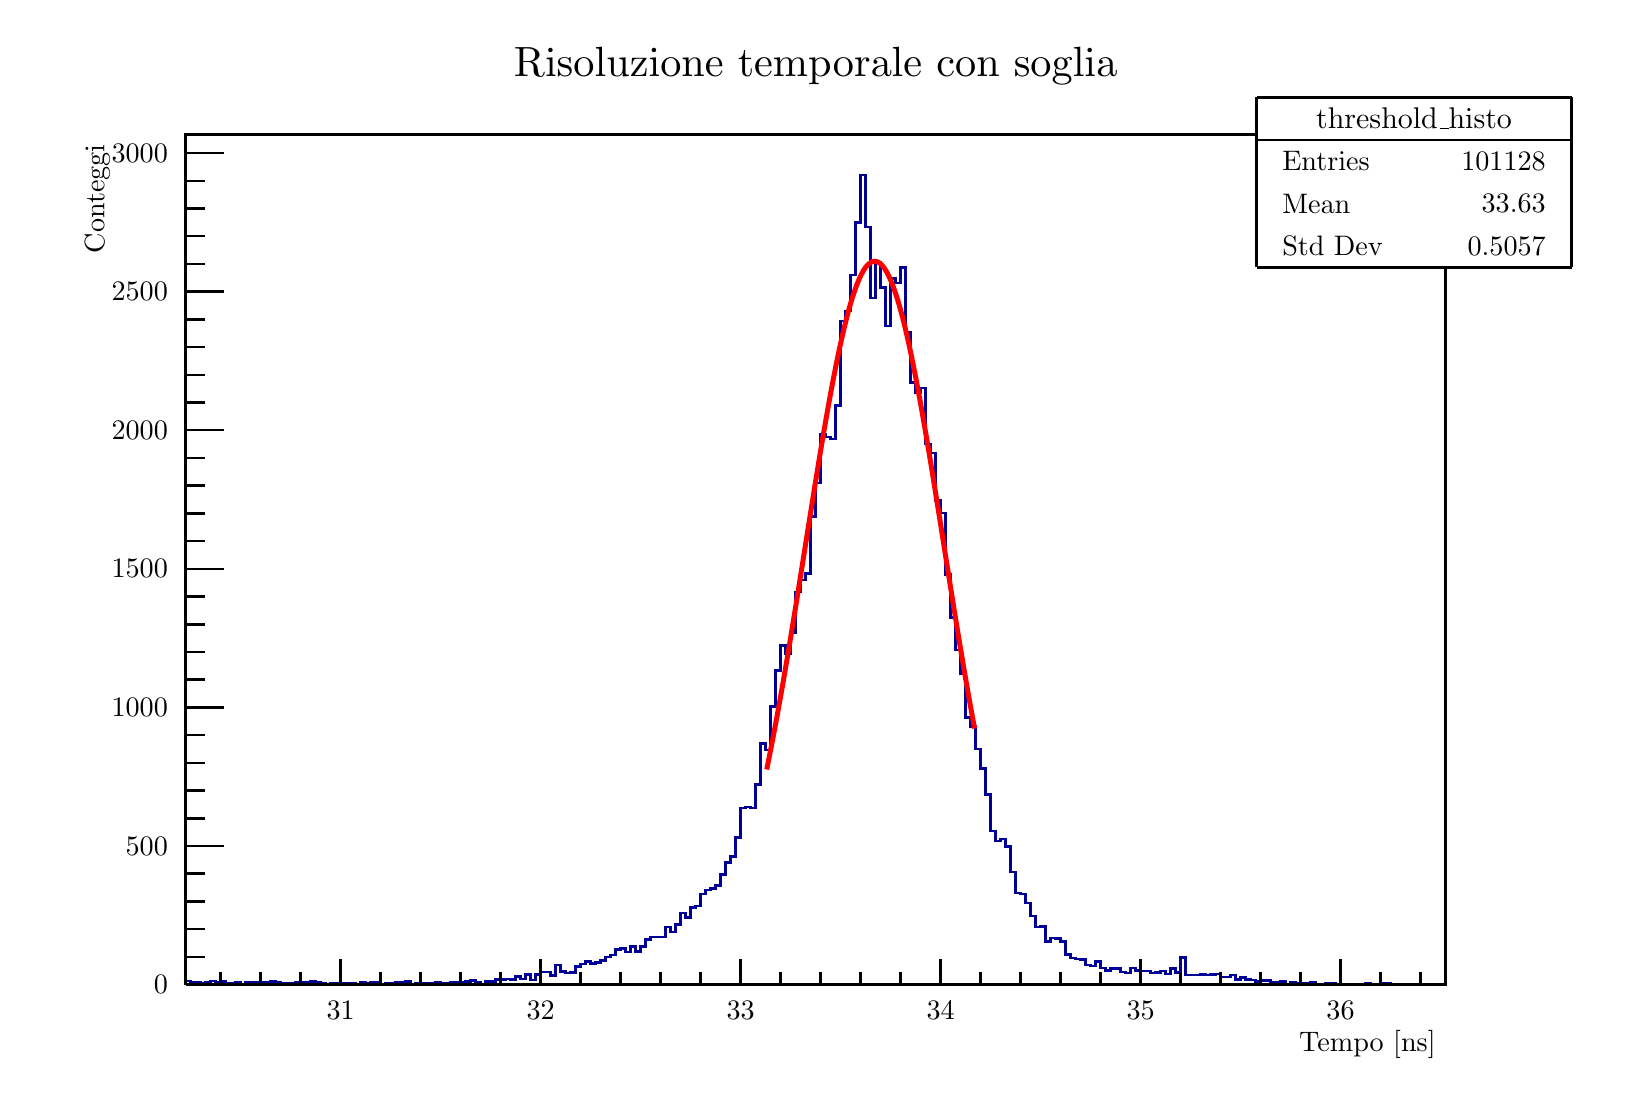
\begin{tikzpicture}
\pgfdeclareplotmark{cross} {
\pgfpathmoveto{\pgfpoint{-0.3\pgfplotmarksize}{\pgfplotmarksize}}
\pgfpathlineto{\pgfpoint{+0.3\pgfplotmarksize}{\pgfplotmarksize}}
\pgfpathlineto{\pgfpoint{+0.3\pgfplotmarksize}{0.3\pgfplotmarksize}}
\pgfpathlineto{\pgfpoint{+1\pgfplotmarksize}{0.3\pgfplotmarksize}}
\pgfpathlineto{\pgfpoint{+1\pgfplotmarksize}{-0.3\pgfplotmarksize}}
\pgfpathlineto{\pgfpoint{+0.3\pgfplotmarksize}{-0.3\pgfplotmarksize}}
\pgfpathlineto{\pgfpoint{+0.3\pgfplotmarksize}{-1.\pgfplotmarksize}}
\pgfpathlineto{\pgfpoint{-0.3\pgfplotmarksize}{-1.\pgfplotmarksize}}
\pgfpathlineto{\pgfpoint{-0.3\pgfplotmarksize}{-0.3\pgfplotmarksize}}
\pgfpathlineto{\pgfpoint{-1.\pgfplotmarksize}{-0.3\pgfplotmarksize}}
\pgfpathlineto{\pgfpoint{-1.\pgfplotmarksize}{0.3\pgfplotmarksize}}
\pgfpathlineto{\pgfpoint{-0.3\pgfplotmarksize}{0.3\pgfplotmarksize}}
\pgfpathclose
\pgfusepathqstroke
}
\pgfdeclareplotmark{cross*} {
\pgfpathmoveto{\pgfpoint{-0.3\pgfplotmarksize}{\pgfplotmarksize}}
\pgfpathlineto{\pgfpoint{+0.3\pgfplotmarksize}{\pgfplotmarksize}}
\pgfpathlineto{\pgfpoint{+0.3\pgfplotmarksize}{0.3\pgfplotmarksize}}
\pgfpathlineto{\pgfpoint{+1\pgfplotmarksize}{0.3\pgfplotmarksize}}
\pgfpathlineto{\pgfpoint{+1\pgfplotmarksize}{-0.3\pgfplotmarksize}}
\pgfpathlineto{\pgfpoint{+0.3\pgfplotmarksize}{-0.3\pgfplotmarksize}}
\pgfpathlineto{\pgfpoint{+0.3\pgfplotmarksize}{-1.\pgfplotmarksize}}
\pgfpathlineto{\pgfpoint{-0.3\pgfplotmarksize}{-1.\pgfplotmarksize}}
\pgfpathlineto{\pgfpoint{-0.3\pgfplotmarksize}{-0.3\pgfplotmarksize}}
\pgfpathlineto{\pgfpoint{-1.\pgfplotmarksize}{-0.3\pgfplotmarksize}}
\pgfpathlineto{\pgfpoint{-1.\pgfplotmarksize}{0.3\pgfplotmarksize}}
\pgfpathlineto{\pgfpoint{-0.3\pgfplotmarksize}{0.3\pgfplotmarksize}}
\pgfpathclose
\pgfusepathqfillstroke
}
\pgfdeclareplotmark{newstar} {
\pgfpathmoveto{\pgfqpoint{0pt}{\pgfplotmarksize}}
\pgfpathlineto{\pgfqpointpolar{44}{0.5\pgfplotmarksize}}
\pgfpathlineto{\pgfqpointpolar{18}{\pgfplotmarksize}}
\pgfpathlineto{\pgfqpointpolar{-20}{0.5\pgfplotmarksize}}
\pgfpathlineto{\pgfqpointpolar{-54}{\pgfplotmarksize}}
\pgfpathlineto{\pgfqpointpolar{-90}{0.5\pgfplotmarksize}}
\pgfpathlineto{\pgfqpointpolar{234}{\pgfplotmarksize}}
\pgfpathlineto{\pgfqpointpolar{198}{0.5\pgfplotmarksize}}
\pgfpathlineto{\pgfqpointpolar{162}{\pgfplotmarksize}}
\pgfpathlineto{\pgfqpointpolar{134}{0.5\pgfplotmarksize}}
\pgfpathclose
\pgfusepathqstroke
}
\pgfdeclareplotmark{newstar*} {
\pgfpathmoveto{\pgfqpoint{0pt}{\pgfplotmarksize}}
\pgfpathlineto{\pgfqpointpolar{44}{0.5\pgfplotmarksize}}
\pgfpathlineto{\pgfqpointpolar{18}{\pgfplotmarksize}}
\pgfpathlineto{\pgfqpointpolar{-20}{0.5\pgfplotmarksize}}
\pgfpathlineto{\pgfqpointpolar{-54}{\pgfplotmarksize}}
\pgfpathlineto{\pgfqpointpolar{-90}{0.5\pgfplotmarksize}}
\pgfpathlineto{\pgfqpointpolar{234}{\pgfplotmarksize}}
\pgfpathlineto{\pgfqpointpolar{198}{0.5\pgfplotmarksize}}
\pgfpathlineto{\pgfqpointpolar{162}{\pgfplotmarksize}}
\pgfpathlineto{\pgfqpointpolar{134}{0.5\pgfplotmarksize}}
\pgfpathclose
\pgfusepathqfillstroke
}
\definecolor{c}{rgb}{1,1,1};
\draw [color=c, fill=c] (0,0) rectangle (20,13.4957);
\draw [color=c, fill=c] (2,1.34957) rectangle (18,12.1461);
\definecolor{c}{rgb}{0,0,0};
\draw [c,line width=0.9] (2,1.34957) -- (2,12.1461) -- (18,12.1461) -- (18,1.34957) -- (2,1.34957);
\definecolor{c}{rgb}{1,1,1};
\draw [color=c, fill=c] (2,1.34957) rectangle (18,12.1461);
\definecolor{c}{rgb}{0,0,0};
\draw [c,line width=0.9] (2,1.34957) -- (2,12.1461) -- (18,12.1461) -- (18,1.34957) -- (2,1.34957);
\definecolor{c}{rgb}{0,0,0.6};
\draw [c,line width=0.9] (2,1.39533) -- (2.06349,1.39533) -- (2.06349,1.37773) -- (2.12698,1.37773) -- (2.12698,1.38125) -- (2.19048,1.38125) -- (2.19048,1.37069) -- (2.25397,1.37069) -- (2.25397,1.38125) -- (2.31746,1.38125) -- (2.31746,1.39533) --
 (2.38095,1.39533) -- (2.38095,1.38477) -- (2.44444,1.38477) -- (2.44444,1.39181) -- (2.50794,1.39181) -- (2.50794,1.37069) -- (2.57143,1.37069) -- (2.57143,1.36365) -- (2.63492,1.36365) -- (2.63492,1.37421) -- (2.69841,1.37421) -- (2.69841,1.36013)
 -- (2.7619,1.36013) -- (2.7619,1.37421) -- (2.8254,1.37421) -- (2.8254,1.37421) -- (2.88889,1.37421) -- (2.88889,1.38477) -- (2.95238,1.38477) -- (2.95238,1.38477) -- (3.01587,1.38477) -- (3.01587,1.38477) -- (3.07937,1.38477) -- (3.07937,1.39181)
 -- (3.14286,1.39181) -- (3.14286,1.37773) -- (3.20635,1.37773) -- (3.20635,1.36717) -- (3.26984,1.36717) -- (3.26984,1.37069) -- (3.33333,1.37069) -- (3.33333,1.37069) -- (3.39683,1.37069) -- (3.39683,1.38125) -- (3.46032,1.38125) --
 (3.46032,1.38125) -- (3.52381,1.38125) -- (3.52381,1.37773) -- (3.5873,1.37773) -- (3.5873,1.38829) -- (3.65079,1.38829) -- (3.65079,1.37421) -- (3.71429,1.37421) -- (3.71429,1.37069) -- (3.77778,1.37069) -- (3.77778,1.36013) -- (3.84127,1.36013) --
 (3.84127,1.36717) -- (3.90476,1.36717) -- (3.90476,1.36365) -- (3.96825,1.36365) -- (3.96825,1.37069) -- (4.03175,1.37069) -- (4.03175,1.36717) -- (4.09524,1.36717) -- (4.09524,1.36717) -- (4.15873,1.36717) -- (4.15873,1.36013) -- (4.22222,1.36013)
 -- (4.22222,1.38125) -- (4.28571,1.38125) -- (4.28571,1.36717) -- (4.34921,1.36717) -- (4.34921,1.38477) -- (4.4127,1.38477) -- (4.4127,1.38477) -- (4.47619,1.38477) -- (4.47619,1.36013) -- (4.53968,1.36013) -- (4.53968,1.37069) -- (4.60317,1.37069)
 -- (4.60317,1.36717) -- (4.66667,1.36717) -- (4.66667,1.38477) -- (4.73016,1.38477) -- (4.73016,1.37773) -- (4.79365,1.37773) -- (4.79365,1.39181) -- (4.85714,1.39181) -- (4.85714,1.36013) -- (4.92064,1.36013) -- (4.92064,1.37069) --
 (4.98413,1.37069) -- (4.98413,1.37069) -- (5.04762,1.37069) -- (5.04762,1.36717) -- (5.11111,1.36717) -- (5.11111,1.36365) -- (5.1746,1.36365) -- (5.1746,1.38477) -- (5.2381,1.38477) -- (5.2381,1.37069) -- (5.30159,1.37069) -- (5.30159,1.37069) --
 (5.36508,1.37069) -- (5.36508,1.37421) -- (5.42857,1.37421) -- (5.42857,1.37773) -- (5.49206,1.37773) -- (5.49206,1.37773) -- (5.55556,1.37773) -- (5.55556,1.39181) -- (5.61905,1.39181) -- (5.61905,1.40237) -- (5.68254,1.40237) -- (5.68254,1.37773)
 -- (5.74603,1.37773) -- (5.74603,1.36013) -- (5.80952,1.36013) -- (5.80952,1.39181) -- (5.87302,1.39181) -- (5.87302,1.39181) -- (5.93651,1.39181) -- (5.93651,1.41293) -- (6,1.41293) -- (6,1.41293) -- (6.06349,1.41293) -- (6.06349,1.42349) --
 (6.12698,1.42349) -- (6.12698,1.41293) -- (6.19048,1.41293) -- (6.19048,1.45166) -- (6.25397,1.45166) -- (6.25397,1.42349) -- (6.31746,1.42349) -- (6.31746,1.4763) -- (6.38095,1.4763) -- (6.38095,1.40589) -- (6.44444,1.40589) -- (6.44444,1.4763) --
 (6.50794,1.4763) -- (6.50794,1.5115) -- (6.57143,1.5115) -- (6.57143,1.5115) -- (6.63492,1.5115) -- (6.63492,1.46222) -- (6.69841,1.46222) -- (6.69841,1.5995) -- (6.7619,1.5995) -- (6.7619,1.51854) -- (6.8254,1.51854) -- (6.8254,1.4939) --
 (6.88889,1.4939) -- (6.88889,1.50446) -- (6.95238,1.50446) -- (6.95238,1.57838) -- (7.01587,1.57838) -- (7.01587,1.61358) -- (7.07937,1.61358) -- (7.07937,1.64174) -- (7.14286,1.64174) -- (7.14286,1.6171) -- (7.20635,1.6171) -- (7.20635,1.62766) --
 (7.26984,1.62766) -- (7.26984,1.65583) -- (7.33333,1.65583) -- (7.33333,1.70159) -- (7.39683,1.70159) -- (7.39683,1.72623) -- (7.46032,1.72623) -- (7.46032,1.79311) -- (7.52381,1.79311) -- (7.52381,1.81071) -- (7.5873,1.81071) -- (7.5873,1.76495) --
 (7.65079,1.76495) -- (7.65079,1.83535) -- (7.71429,1.83535) -- (7.71429,1.77199) -- (7.77778,1.77199) -- (7.77778,1.83535) -- (7.84127,1.83535) -- (7.84127,1.92336) -- (7.90476,1.92336) -- (7.90476,1.95504) -- (7.96825,1.95504) -- (7.96825,1.95504)
 -- (8.03175,1.95504) -- (8.03175,1.95504) -- (8.09524,1.95504) -- (8.09524,2.07825) -- (8.15873,2.07825) -- (8.15873,2.01488) -- (8.22222,2.01488) -- (8.22222,2.11345) -- (8.28571,2.11345) -- (8.28571,2.2613) -- (8.34921,2.2613) -- (8.34921,2.20497)
 -- (8.4127,2.20497) -- (8.4127,2.32818) -- (8.47619,2.32818) -- (8.47619,2.3493) -- (8.53968,2.3493) -- (8.53968,2.50067) -- (8.60317,2.50067) -- (8.60317,2.54995) -- (8.66667,2.54995) -- (8.66667,2.57107) -- (8.73016,2.57107) -- (8.73016,2.60627)
 -- (8.79365,2.60627) -- (8.79365,2.7506) -- (8.85714,2.7506) -- (8.85714,2.89845) -- (8.92064,2.89845) -- (8.92064,2.97941) -- (8.98413,2.97941) -- (8.98413,3.21526) -- (9.04762,3.21526) -- (9.04762,3.59544) -- (9.11111,3.59544) -- (9.11111,3.60248)
 -- (9.1746,3.60248) -- (9.1746,3.59192) -- (9.2381,3.59192) -- (9.2381,3.89114) -- (9.30159,3.89114) -- (9.30159,4.4086) -- (9.36508,4.4086) -- (9.36508,4.32764) -- (9.42857,4.32764) -- (9.42857,4.88383) -- (9.49206,4.88383) -- (9.49206,5.34145) --
 (9.55556,5.34145) -- (9.55556,5.65475) -- (9.61905,5.65475) -- (9.61905,5.55266) -- (9.68254,5.55266) -- (9.68254,5.81668) -- (9.74603,5.81668) -- (9.74603,6.33414) -- (9.80952,6.33414) -- (9.80952,6.48903) -- (9.87302,6.48903) -- (9.87302,6.57351)
 -- (9.93651,6.57351) -- (9.93651,7.29515) -- (10,7.29515) -- (10,7.72109) -- (10.0635,7.72109) -- (10.0635,8.34064) -- (10.127,8.34064) -- (10.127,8.30192) -- (10.1905,8.30192) -- (10.1905,8.2808) -- (10.254,8.2808) -- (10.254,8.70674) --
 (10.3175,8.70674) -- (10.3175,9.7804) -- (10.381,9.7804) -- (10.381,9.9036) -- (10.4444,9.9036) -- (10.4444,10.3647) -- (10.5079,10.3647) -- (10.5079,11.0265) -- (10.5714,11.0265) -- (10.5714,11.632) -- (10.6349,11.632) -- (10.6349,10.9702) --
 (10.6984,10.9702) -- (10.6984,10.0726) -- (10.7619,10.0726) -- (10.7619,10.5232) -- (10.8254,10.5232) -- (10.8254,10.2028) -- (10.8889,10.2028) -- (10.8889,9.71703) -- (10.9524,9.71703) -- (10.9524,10.3155) -- (11.0159,10.3155) -- (11.0159,10.2627)
 -- (11.0794,10.2627) -- (11.0794,10.4563) -- (11.1429,10.4563) -- (11.1429,9.62903) -- (11.2063,9.62903) -- (11.2063,8.99892) -- (11.2698,8.99892) -- (11.2698,8.86867) -- (11.3333,8.86867) -- (11.3333,8.92499) -- (11.3968,8.92499) --
 (11.3968,8.21744) -- (11.4603,8.21744) -- (11.4603,8.10127) -- (11.5238,8.10127) -- (11.5238,7.49932) -- (11.5873,7.49932) -- (11.5873,7.34091) -- (11.6508,7.34091) -- (11.6508,6.55943) -- (11.7143,6.55943) -- (11.7143,6.01029) -- (11.7778,6.01029)
 -- (11.7778,5.60194) -- (11.8413,5.60194) -- (11.8413,5.29921) -- (11.9048,5.29921) -- (11.9048,4.74302) -- (11.9683,4.74302) -- (11.9683,4.62686) -- (12.0317,4.62686) -- (12.0317,4.34172) -- (12.0952,4.34172) -- (12.0952,4.09179) --
 (12.1587,4.09179) -- (12.1587,3.76441) -- (12.2222,3.76441) -- (12.2222,3.30327) -- (12.2857,3.30327) -- (12.2857,3.17654) -- (12.3492,3.17654) -- (12.3492,3.20118) -- (12.4127,3.20118) -- (12.4127,3.10262) -- (12.4762,3.10262) -- (12.4762,2.77876)
 -- (12.5397,2.77876) -- (12.5397,2.51123) -- (12.6032,2.51123) -- (12.6032,2.50067) -- (12.6667,2.50067) -- (12.6667,2.3845) -- (12.7302,2.3845) -- (12.7302,2.21905) -- (12.7937,2.21905) -- (12.7937,2.07825) -- (12.8571,2.07825) -- (12.8571,2.08529)
 -- (12.9206,2.08529) -- (12.9206,1.89872) -- (12.9841,1.89872) -- (12.9841,1.94448) -- (13.0476,1.94448) -- (13.0476,1.93392) -- (13.1111,1.93392) -- (13.1111,1.8952) -- (13.1746,1.8952) -- (13.1746,1.72975) -- (13.2381,1.72975) -- (13.2381,1.68751)
 -- (13.3016,1.68751) -- (13.3016,1.67695) -- (13.3651,1.67695) -- (13.3651,1.66991) -- (13.4286,1.66991) -- (13.4286,1.59598) -- (13.4921,1.59598) -- (13.4921,1.58894) -- (13.5556,1.58894) -- (13.5556,1.64174) -- (13.619,1.64174) -- (13.619,1.56078)
 -- (13.6825,1.56078) -- (13.6825,1.5291) -- (13.746,1.5291) -- (13.746,1.55726) -- (13.8095,1.55726) -- (13.8095,1.55374) -- (13.873,1.55374) -- (13.873,1.50798) -- (13.9365,1.50798) -- (13.9365,1.4939) -- (14,1.4939) -- (14,1.56078) --
 (14.0635,1.56078) -- (14.0635,1.5291) -- (14.127,1.5291) -- (14.127,1.52206) -- (14.1905,1.52206) -- (14.1905,1.52558) -- (14.254,1.52558) -- (14.254,1.49742) -- (14.3175,1.49742) -- (14.3175,1.50446) -- (14.381,1.50446) -- (14.381,1.52558) --
 (14.4444,1.52558) -- (14.4444,1.48686) -- (14.5079,1.48686) -- (14.5079,1.55374) -- (14.5714,1.55374) -- (14.5714,1.50094) -- (14.6349,1.50094) -- (14.6349,1.69103) -- (14.6984,1.69103) -- (14.6984,1.47278) -- (14.7619,1.47278) -- (14.7619,1.47278)
 -- (14.8254,1.47278) -- (14.8254,1.46926) -- (14.8889,1.46926) -- (14.8889,1.47982) -- (14.9524,1.47982) -- (14.9524,1.46926) -- (15.0159,1.46926) -- (15.0159,1.4763) -- (15.0794,1.4763) -- (15.0794,1.48686) -- (15.1429,1.48686) -- (15.1429,1.44814)
 -- (15.2063,1.44814) -- (15.2063,1.44814) -- (15.2698,1.44814) -- (15.2698,1.47278) -- (15.3333,1.47278) -- (15.3333,1.41645) -- (15.3968,1.41645) -- (15.3968,1.43757) -- (15.4603,1.43757) -- (15.4603,1.41645) -- (15.5238,1.41645) --
 (15.5238,1.40941) -- (15.5873,1.40941) -- (15.5873,1.39181) -- (15.6508,1.39181) -- (15.6508,1.40237) -- (15.7143,1.40237) -- (15.7143,1.40237) -- (15.7778,1.40237) -- (15.7778,1.37773) -- (15.8413,1.37773) -- (15.8413,1.38125) -- (15.9048,1.38125)
 -- (15.9048,1.38829) -- (15.9683,1.38829) -- (15.9683,1.36013) -- (16.0317,1.36013) -- (16.0317,1.37421) -- (16.0952,1.37421) -- (16.0952,1.37069) -- (16.1587,1.37069) -- (16.1587,1.37069) -- (16.2222,1.37069) -- (16.2222,1.36365) --
 (16.2857,1.36365) -- (16.2857,1.37421) -- (16.3492,1.37421) -- (16.3492,1.35661) -- (16.4127,1.35661) -- (16.4127,1.35661) -- (16.4762,1.35661) -- (16.4762,1.36717) -- (16.5397,1.36717) -- (16.5397,1.36365) -- (16.6032,1.36365) -- (16.6032,1.35309)
 -- (16.6667,1.35309) -- (16.6667,1.35661) -- (16.7302,1.35661) -- (16.7302,1.35309) -- (16.7937,1.35309) -- (16.7937,1.35309) -- (16.8571,1.35309) -- (16.8571,1.35661) -- (16.9206,1.35661) -- (16.9206,1.35309) -- (16.9841,1.35309) --
 (16.9841,1.36365) -- (17.0476,1.36365) -- (17.0476,1.35309) -- (17.1111,1.35309) -- (17.1111,1.35309) -- (17.1746,1.35309) -- (17.1746,1.36717) -- (17.2381,1.36717) -- (17.2381,1.36365) -- (17.3016,1.36365) -- (17.3016,1.35309) -- (17.3651,1.35309)
 -- (17.3651,1.36013) -- (17.4286,1.36013) -- (17.4286,1.35661) -- (17.4921,1.35661) -- (17.4921,1.35309) -- (17.5556,1.35309) -- (17.5556,1.36013) -- (17.619,1.36013) -- (17.619,1.35309) -- (17.6825,1.35309) -- (17.6825,1.34957) -- (17.746,1.34957)
 -- (17.746,1.35661) -- (17.8095,1.35661) -- (17.8095,1.35309) -- (17.873,1.35309) -- (17.873,1.34957) -- (17.9365,1.34957) -- (17.9365,1.35309) -- (18,1.35309);
\definecolor{c}{rgb}{1,1,1};
\draw [color=c, fill=c] (15.6,10.4592) rectangle (19.6,12.6185);
\definecolor{c}{rgb}{0,0,0};
\draw [c,line width=0.9] (15.6,10.4592) -- (19.6,10.4592);
\draw [c,line width=0.9] (19.6,10.4592) -- (19.6,12.6185);
\draw [c,line width=0.9] (19.6,12.6185) -- (15.6,12.6185);
\draw [c,line width=0.9] (15.6,12.6185) -- (15.6,10.4592);
\draw (17.6,12.3486) node[scale=1.08185, color=c, rotate=0]{threshold\_histo};
\draw [c,line width=0.9] (15.6,12.0787) -- (19.6,12.0787);
\draw [anchor= west] (15.8,11.8087) node[scale=1.01821, color=c, rotate=0]{Entries };
\draw [anchor= east] (19.4,11.8087) node[scale=1.01821, color=c, rotate=0]{ 101128};
\draw [anchor= west] (15.8,11.2689) node[scale=1.01821, color=c, rotate=0]{Mean  };
\draw [anchor= east] (19.4,11.2689) node[scale=1.01821, color=c, rotate=0]{  33.63};
\draw [anchor= west] (15.8,10.7291) node[scale=1.01821, color=c, rotate=0]{Std Dev   };
\draw [anchor= east] (19.4,10.7291) node[scale=1.01821, color=c, rotate=0]{ 0.5057};
\definecolor{c}{rgb}{1,0,0};
\draw [c,line width=1.8] (9.37841,4.0812) -- (9.40508,4.21184) -- (9.43175,4.34597) -- (9.45841,4.48351) -- (9.48508,4.62436) -- (9.51175,4.76841) -- (9.53841,4.91551) -- (9.56508,5.06554) -- (9.59175,5.21833) -- (9.61841,5.3737) -- (9.64508,5.53148)
 -- (9.67175,5.69146) -- (9.69841,5.85343) -- (9.72508,6.01715) -- (9.75175,6.18239) -- (9.77841,6.34889) -- (9.80508,6.51639) -- (9.83175,6.6846) -- (9.85841,6.85324) -- (9.88508,7.022) -- (9.91175,7.19058) -- (9.93841,7.35865) -- (9.96508,7.52589)
 -- (9.99175,7.69196) -- (10.0184,7.85653) -- (10.0451,8.01925) -- (10.0717,8.17976) -- (10.0984,8.33773) -- (10.1251,8.49279) -- (10.1517,8.6446) -- (10.1784,8.79281) -- (10.2051,8.93706) -- (10.2317,9.07701) -- (10.2584,9.21233) --
 (10.2851,9.34269) -- (10.3117,9.46776) -- (10.3384,9.58722) -- (10.3651,9.70077) -- (10.3917,9.80813) -- (10.4184,9.90902) -- (10.4451,10.0032) -- (10.4717,10.0903) -- (10.4984,10.1703) -- (10.5251,10.2428) -- (10.5517,10.3077) -- (10.5784,10.3647)
 -- (10.6051,10.4139) -- (10.6317,10.4549) -- (10.6584,10.4878) -- (10.6851,10.5123);
\draw [c,line width=1.8] (10.6851,10.5123) -- (10.7117,10.5285) -- (10.7384,10.5363) -- (10.7651,10.5356) -- (10.7917,10.5266) -- (10.8184,10.5091) -- (10.8451,10.4833) -- (10.8717,10.4492) -- (10.8984,10.407) -- (10.9251,10.3566) --
 (10.9517,10.2984) -- (10.9784,10.2323) -- (11.0051,10.1587) -- (11.0317,10.0776) -- (11.0584,9.98942) -- (11.0851,9.89424) -- (11.1117,9.79236) -- (11.1384,9.68405) -- (11.1651,9.56959) -- (11.1917,9.44926) -- (11.2184,9.32338) -- (11.2451,9.19225)
 -- (11.2717,9.05621) -- (11.2984,8.91559) -- (11.3251,8.77072) -- (11.3517,8.62195) -- (11.3784,8.46962) -- (11.4051,8.3141) -- (11.4317,8.15573) -- (11.4584,7.99486) -- (11.4851,7.83184) -- (11.5117,7.66703) -- (11.5384,7.50076) --
 (11.5651,7.33337) -- (11.5917,7.1652) -- (11.6184,6.99658) -- (11.6451,6.82781) -- (11.6717,6.65922) -- (11.6984,6.4911) -- (11.7251,6.32373) -- (11.7517,6.1574) -- (11.7784,5.99238) -- (11.8051,5.8289) -- (11.8317,5.66722) -- (11.8584,5.50756) --
 (11.8851,5.35013) -- (11.9117,5.19513) -- (11.9384,5.04275) -- (11.9651,4.89316) -- (11.9917,4.7465);
\draw [c,line width=1.8] (11.9917,4.7465) -- (12.0184,4.60293);
\definecolor{c}{rgb}{0,0,0};
\draw [c,line width=0.9] (2,1.34957) -- (18,1.34957);
\draw [anchor= east] (18,0.593811) node[scale=1.01821, color=c, rotate=0]{Tempo [ns]};
\draw [c,line width=0.9] (3.96825,1.67347) -- (3.96825,1.34957);
\draw [c,line width=0.9] (4.47619,1.51152) -- (4.47619,1.34957);
\draw [c,line width=0.9] (4.98413,1.51152) -- (4.98413,1.34957);
\draw [c,line width=0.9] (5.49206,1.51152) -- (5.49206,1.34957);
\draw [c,line width=0.9] (6,1.51152) -- (6,1.34957);
\draw [c,line width=0.9] (6.50794,1.67347) -- (6.50794,1.34957);
\draw [c,line width=0.9] (7.01587,1.51152) -- (7.01587,1.34957);
\draw [c,line width=0.9] (7.52381,1.51152) -- (7.52381,1.34957);
\draw [c,line width=0.9] (8.03175,1.51152) -- (8.03175,1.34957);
\draw [c,line width=0.9] (8.53968,1.51152) -- (8.53968,1.34957);
\draw [c,line width=0.9] (9.04762,1.67347) -- (9.04762,1.34957);
\draw [c,line width=0.9] (9.55556,1.51152) -- (9.55556,1.34957);
\draw [c,line width=0.9] (10.0635,1.51152) -- (10.0635,1.34957);
\draw [c,line width=0.9] (10.5714,1.51152) -- (10.5714,1.34957);
\draw [c,line width=0.9] (11.0794,1.51152) -- (11.0794,1.34957);
\draw [c,line width=0.9] (11.5873,1.67347) -- (11.5873,1.34957);
\draw [c,line width=0.9] (12.0952,1.51152) -- (12.0952,1.34957);
\draw [c,line width=0.9] (12.6032,1.51152) -- (12.6032,1.34957);
\draw [c,line width=0.9] (13.1111,1.51152) -- (13.1111,1.34957);
\draw [c,line width=0.9] (13.619,1.51152) -- (13.619,1.34957);
\draw [c,line width=0.9] (14.127,1.67347) -- (14.127,1.34957);
\draw [c,line width=0.9] (14.6349,1.51152) -- (14.6349,1.34957);
\draw [c,line width=0.9] (15.1429,1.51152) -- (15.1429,1.34957);
\draw [c,line width=0.9] (15.6508,1.51152) -- (15.6508,1.34957);
\draw [c,line width=0.9] (16.1587,1.51152) -- (16.1587,1.34957);
\draw [c,line width=0.9] (16.6667,1.67347) -- (16.6667,1.34957);
\draw [c,line width=0.9] (3.96825,1.67347) -- (3.96825,1.34957);
\draw [c,line width=0.9] (3.46032,1.51152) -- (3.46032,1.34957);
\draw [c,line width=0.9] (2.95238,1.51152) -- (2.95238,1.34957);
\draw [c,line width=0.9] (2.44444,1.51152) -- (2.44444,1.34957);
\draw [c,line width=0.9] (16.6667,1.67347) -- (16.6667,1.34957);
\draw [c,line width=0.9] (17.1746,1.51152) -- (17.1746,1.34957);
\draw [c,line width=0.9] (17.6825,1.51152) -- (17.6825,1.34957);
\draw [anchor=base] (3.96825,0.904212) node[scale=1.01821, color=c, rotate=0]{31};
\draw [anchor=base] (6.50794,0.904212) node[scale=1.01821, color=c, rotate=0]{32};
\draw [anchor=base] (9.04762,0.904212) node[scale=1.01821, color=c, rotate=0]{33};
\draw [anchor=base] (11.5873,0.904212) node[scale=1.01821, color=c, rotate=0]{34};
\draw [anchor=base] (14.127,0.904212) node[scale=1.01821, color=c, rotate=0]{35};
\draw [anchor=base] (16.6667,0.904212) node[scale=1.01821, color=c, rotate=0]{36};
\draw [c,line width=0.9] (2,1.34957) -- (2,12.1461);
\draw [anchor= east] (0.88,12.1461) node[scale=1.01821, color=c, rotate=90]{Conteggi};
\draw [c,line width=0.9] (2.48,1.34957) -- (2,1.34957);
\draw [c,line width=0.9] (2.24,1.70159) -- (2,1.70159);
\draw [c,line width=0.9] (2.24,2.05361) -- (2,2.05361);
\draw [c,line width=0.9] (2.24,2.40562) -- (2,2.40562);
\draw [c,line width=0.9] (2.24,2.75764) -- (2,2.75764);
\draw [c,line width=0.9] (2.48,3.10966) -- (2,3.10966);
\draw [c,line width=0.9] (2.24,3.46168) -- (2,3.46168);
\draw [c,line width=0.9] (2.24,3.81369) -- (2,3.81369);
\draw [c,line width=0.9] (2.24,4.16571) -- (2,4.16571);
\draw [c,line width=0.9] (2.24,4.51773) -- (2,4.51773);
\draw [c,line width=0.9] (2.48,4.86975) -- (2,4.86975);
\draw [c,line width=0.9] (2.24,5.22177) -- (2,5.22177);
\draw [c,line width=0.9] (2.24,5.57378) -- (2,5.57378);
\draw [c,line width=0.9] (2.24,5.9258) -- (2,5.9258);
\draw [c,line width=0.9] (2.24,6.27782) -- (2,6.27782);
\draw [c,line width=0.9] (2.48,6.62984) -- (2,6.62984);
\draw [c,line width=0.9] (2.24,6.98185) -- (2,6.98185);
\draw [c,line width=0.9] (2.24,7.33387) -- (2,7.33387);
\draw [c,line width=0.9] (2.24,7.68589) -- (2,7.68589);
\draw [c,line width=0.9] (2.24,8.03791) -- (2,8.03791);
\draw [c,line width=0.9] (2.48,8.38993) -- (2,8.38993);
\draw [c,line width=0.9] (2.24,8.74194) -- (2,8.74194);
\draw [c,line width=0.9] (2.24,9.09396) -- (2,9.09396);
\draw [c,line width=0.9] (2.24,9.44598) -- (2,9.44598);
\draw [c,line width=0.9] (2.24,9.798) -- (2,9.798);
\draw [c,line width=0.9] (2.48,10.15) -- (2,10.15);
\draw [c,line width=0.9] (2.24,10.502) -- (2,10.502);
\draw [c,line width=0.9] (2.24,10.8541) -- (2,10.8541);
\draw [c,line width=0.9] (2.24,11.2061) -- (2,11.2061);
\draw [c,line width=0.9] (2.24,11.5581) -- (2,11.5581);
\draw [c,line width=0.9] (2.48,11.9101) -- (2,11.9101);
\draw [c,line width=0.9] (2.48,11.9101) -- (2,11.9101);
\draw [anchor= east] (1.9,1.34957) node[scale=1.01821, color=c, rotate=0]{0};
\draw [anchor= east] (1.9,3.10966) node[scale=1.01821, color=c, rotate=0]{500};
\draw [anchor= east] (1.9,4.86975) node[scale=1.01821, color=c, rotate=0]{1000};
\draw [anchor= east] (1.9,6.62984) node[scale=1.01821, color=c, rotate=0]{1500};
\draw [anchor= east] (1.9,8.38993) node[scale=1.01821, color=c, rotate=0]{2000};
\draw [anchor= east] (1.9,10.15) node[scale=1.01821, color=c, rotate=0]{2500};
\draw [anchor= east] (1.9,11.9101) node[scale=1.01821, color=c, rotate=0]{3000};
\definecolor{c}{rgb}{1,1,1};
\draw [color=c, fill=c] (15.6,10.4592) rectangle (19.6,12.6185);
\definecolor{c}{rgb}{0,0,0};
\draw [c,line width=0.9] (15.6,10.4592) -- (19.6,10.4592);
\draw [c,line width=0.9] (19.6,10.4592) -- (19.6,12.6185);
\draw [c,line width=0.9] (19.6,12.6185) -- (15.6,12.6185);
\draw [c,line width=0.9] (15.6,12.6185) -- (15.6,10.4592);
\draw (17.6,12.3486) node[scale=1.08185, color=c, rotate=0]{threshold\_histo};
\draw [c,line width=0.9] (15.6,12.0787) -- (19.6,12.0787);
\draw [anchor= west] (15.8,11.8087) node[scale=1.01821, color=c, rotate=0]{Entries };
\draw [anchor= east] (19.4,11.8087) node[scale=1.01821, color=c, rotate=0]{ 101128};
\draw [anchor= west] (15.8,11.2689) node[scale=1.01821, color=c, rotate=0]{Mean  };
\draw [anchor= east] (19.4,11.2689) node[scale=1.01821, color=c, rotate=0]{  33.63};
\draw [anchor= west] (15.8,10.7291) node[scale=1.01821, color=c, rotate=0]{Std Dev   };
\draw [anchor= east] (19.4,10.7291) node[scale=1.01821, color=c, rotate=0]{ 0.5057};
\draw (10,13.0156) node[scale=1.52731, color=c, rotate=0]{Risoluzione temporale con soglia};
\end{tikzpicture}

%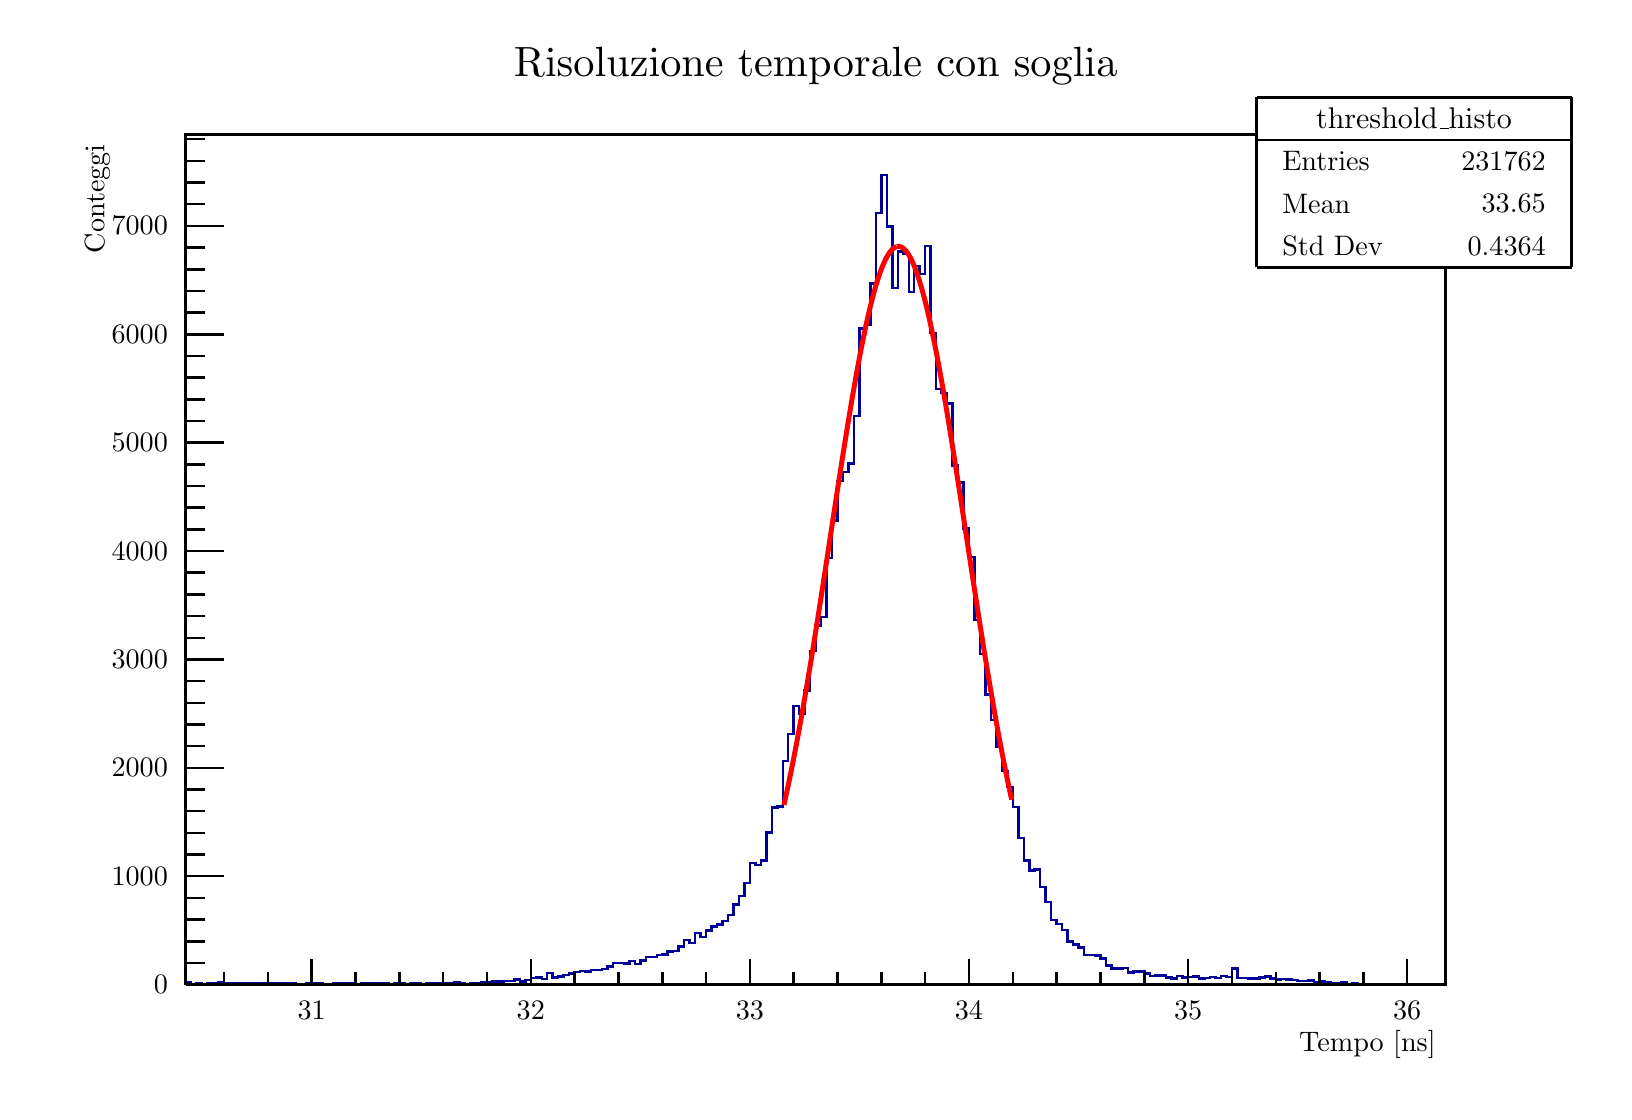
\begin{tikzpicture}
\pgfdeclareplotmark{cross} {
\pgfpathmoveto{\pgfpoint{-0.3\pgfplotmarksize}{\pgfplotmarksize}}
\pgfpathlineto{\pgfpoint{+0.3\pgfplotmarksize}{\pgfplotmarksize}}
\pgfpathlineto{\pgfpoint{+0.3\pgfplotmarksize}{0.3\pgfplotmarksize}}
\pgfpathlineto{\pgfpoint{+1\pgfplotmarksize}{0.3\pgfplotmarksize}}
\pgfpathlineto{\pgfpoint{+1\pgfplotmarksize}{-0.3\pgfplotmarksize}}
\pgfpathlineto{\pgfpoint{+0.3\pgfplotmarksize}{-0.3\pgfplotmarksize}}
\pgfpathlineto{\pgfpoint{+0.3\pgfplotmarksize}{-1.\pgfplotmarksize}}
\pgfpathlineto{\pgfpoint{-0.3\pgfplotmarksize}{-1.\pgfplotmarksize}}
\pgfpathlineto{\pgfpoint{-0.3\pgfplotmarksize}{-0.3\pgfplotmarksize}}
\pgfpathlineto{\pgfpoint{-1.\pgfplotmarksize}{-0.3\pgfplotmarksize}}
\pgfpathlineto{\pgfpoint{-1.\pgfplotmarksize}{0.3\pgfplotmarksize}}
\pgfpathlineto{\pgfpoint{-0.3\pgfplotmarksize}{0.3\pgfplotmarksize}}
\pgfpathclose
\pgfusepathqstroke
}
\pgfdeclareplotmark{cross*} {
\pgfpathmoveto{\pgfpoint{-0.3\pgfplotmarksize}{\pgfplotmarksize}}
\pgfpathlineto{\pgfpoint{+0.3\pgfplotmarksize}{\pgfplotmarksize}}
\pgfpathlineto{\pgfpoint{+0.3\pgfplotmarksize}{0.3\pgfplotmarksize}}
\pgfpathlineto{\pgfpoint{+1\pgfplotmarksize}{0.3\pgfplotmarksize}}
\pgfpathlineto{\pgfpoint{+1\pgfplotmarksize}{-0.3\pgfplotmarksize}}
\pgfpathlineto{\pgfpoint{+0.3\pgfplotmarksize}{-0.3\pgfplotmarksize}}
\pgfpathlineto{\pgfpoint{+0.3\pgfplotmarksize}{-1.\pgfplotmarksize}}
\pgfpathlineto{\pgfpoint{-0.3\pgfplotmarksize}{-1.\pgfplotmarksize}}
\pgfpathlineto{\pgfpoint{-0.3\pgfplotmarksize}{-0.3\pgfplotmarksize}}
\pgfpathlineto{\pgfpoint{-1.\pgfplotmarksize}{-0.3\pgfplotmarksize}}
\pgfpathlineto{\pgfpoint{-1.\pgfplotmarksize}{0.3\pgfplotmarksize}}
\pgfpathlineto{\pgfpoint{-0.3\pgfplotmarksize}{0.3\pgfplotmarksize}}
\pgfpathclose
\pgfusepathqfillstroke
}
\pgfdeclareplotmark{newstar} {
\pgfpathmoveto{\pgfqpoint{0pt}{\pgfplotmarksize}}
\pgfpathlineto{\pgfqpointpolar{44}{0.5\pgfplotmarksize}}
\pgfpathlineto{\pgfqpointpolar{18}{\pgfplotmarksize}}
\pgfpathlineto{\pgfqpointpolar{-20}{0.5\pgfplotmarksize}}
\pgfpathlineto{\pgfqpointpolar{-54}{\pgfplotmarksize}}
\pgfpathlineto{\pgfqpointpolar{-90}{0.5\pgfplotmarksize}}
\pgfpathlineto{\pgfqpointpolar{234}{\pgfplotmarksize}}
\pgfpathlineto{\pgfqpointpolar{198}{0.5\pgfplotmarksize}}
\pgfpathlineto{\pgfqpointpolar{162}{\pgfplotmarksize}}
\pgfpathlineto{\pgfqpointpolar{134}{0.5\pgfplotmarksize}}
\pgfpathclose
\pgfusepathqstroke
}
\pgfdeclareplotmark{newstar*} {
\pgfpathmoveto{\pgfqpoint{0pt}{\pgfplotmarksize}}
\pgfpathlineto{\pgfqpointpolar{44}{0.5\pgfplotmarksize}}
\pgfpathlineto{\pgfqpointpolar{18}{\pgfplotmarksize}}
\pgfpathlineto{\pgfqpointpolar{-20}{0.5\pgfplotmarksize}}
\pgfpathlineto{\pgfqpointpolar{-54}{\pgfplotmarksize}}
\pgfpathlineto{\pgfqpointpolar{-90}{0.5\pgfplotmarksize}}
\pgfpathlineto{\pgfqpointpolar{234}{\pgfplotmarksize}}
\pgfpathlineto{\pgfqpointpolar{198}{0.5\pgfplotmarksize}}
\pgfpathlineto{\pgfqpointpolar{162}{\pgfplotmarksize}}
\pgfpathlineto{\pgfqpointpolar{134}{0.5\pgfplotmarksize}}
\pgfpathclose
\pgfusepathqfillstroke
}
\definecolor{c}{rgb}{1,1,1};
\draw [color=c, fill=c] (0,0) rectangle (20,13.4957);
\draw [color=c, fill=c] (2,1.34957) rectangle (18,12.1461);
\definecolor{c}{rgb}{0,0,0};
\draw [c,line width=0.9] (2,1.34957) -- (2,12.1461) -- (18,12.1461) -- (18,1.34957) -- (2,1.34957);
\definecolor{c}{rgb}{1,1,1};
\draw [color=c, fill=c] (2,1.34957) rectangle (18,12.1461);
\definecolor{c}{rgb}{0,0,0};
\draw [c,line width=0.9] (2,1.34957) -- (2,12.1461) -- (18,12.1461) -- (18,1.34957) -- (2,1.34957);
\definecolor{c}{rgb}{0,0,0.6};
\draw [c,line width=0.9] (2,1.37848) -- (2.06957,1.37848) -- (2.06957,1.36058) -- (2.13913,1.36058) -- (2.13913,1.37022) -- (2.2087,1.37022) -- (2.2087,1.35783) -- (2.27826,1.35783) -- (2.27826,1.36609) -- (2.34783,1.36609) -- (2.34783,1.36471) --
 (2.41739,1.36471) -- (2.41739,1.37572) -- (2.48696,1.37572) -- (2.48696,1.37022) -- (2.55652,1.37022) -- (2.55652,1.36746) -- (2.62609,1.36746) -- (2.62609,1.37159) -- (2.69565,1.37159) -- (2.69565,1.36746) -- (2.76522,1.36746) -- (2.76522,1.36334)
 -- (2.83478,1.36334) -- (2.83478,1.36884) -- (2.90435,1.36884) -- (2.90435,1.36471) -- (2.97391,1.36471) -- (2.97391,1.37297) -- (3.04348,1.37297) -- (3.04348,1.37022) -- (3.11304,1.37022) -- (3.11304,1.36334) -- (3.18261,1.36334) --
 (3.18261,1.37159) -- (3.25217,1.37159) -- (3.25217,1.36746) -- (3.32174,1.36746) -- (3.32174,1.36196) -- (3.3913,1.36196) -- (3.3913,1.35783) -- (3.46087,1.35783) -- (3.46087,1.36058) -- (3.53043,1.36058) -- (3.53043,1.36196) -- (3.6,1.36196) --
 (3.6,1.36884) -- (3.66957,1.36884) -- (3.66957,1.36196) -- (3.73913,1.36196) -- (3.73913,1.35783) -- (3.8087,1.35783) -- (3.8087,1.35645) -- (3.87826,1.35645) -- (3.87826,1.36746) -- (3.94783,1.36746) -- (3.94783,1.36196) -- (4.01739,1.36196) --
 (4.01739,1.37159) -- (4.08696,1.37159) -- (4.08696,1.36746) -- (4.15652,1.36746) -- (4.15652,1.35783) -- (4.22609,1.35783) -- (4.22609,1.36196) -- (4.29565,1.36196) -- (4.29565,1.36334) -- (4.36522,1.36334) -- (4.36522,1.36334) -- (4.43478,1.36334)
 -- (4.43478,1.36334) -- (4.50435,1.36334) -- (4.50435,1.36746) -- (4.57391,1.36746) -- (4.57391,1.35645) -- (4.64348,1.35645) -- (4.64348,1.36471) -- (4.71304,1.36471) -- (4.71304,1.36334) -- (4.78261,1.36334) -- (4.78261,1.35783) --
 (4.85217,1.35783) -- (4.85217,1.36196) -- (4.92174,1.36196) -- (4.92174,1.36884) -- (4.9913,1.36884) -- (4.9913,1.36058) -- (5.06087,1.36058) -- (5.06087,1.36196) -- (5.13043,1.36196) -- (5.13043,1.36334) -- (5.2,1.36334) -- (5.2,1.36471) --
 (5.26957,1.36471) -- (5.26957,1.36884) -- (5.33913,1.36884) -- (5.33913,1.36884) -- (5.4087,1.36884) -- (5.4087,1.3771) -- (5.47826,1.3771) -- (5.47826,1.36196) -- (5.54783,1.36196) -- (5.54783,1.36058) -- (5.61739,1.36058) -- (5.61739,1.37022) --
 (5.68696,1.37022) -- (5.68696,1.37159) -- (5.75652,1.37159) -- (5.75652,1.38536) -- (5.82609,1.38536) -- (5.82609,1.38123) -- (5.89565,1.38123) -- (5.89565,1.38949) -- (5.96522,1.38949) -- (5.96522,1.38674) -- (6.03478,1.38674) -- (6.03478,1.39499)
 -- (6.10435,1.39499) -- (6.10435,1.39499) -- (6.17391,1.39499) -- (6.17391,1.41702) -- (6.24348,1.41702) -- (6.24348,1.38674) -- (6.31304,1.38674) -- (6.31304,1.41014) -- (6.38261,1.41014) -- (6.38261,1.43491) -- (6.45217,1.43491) --
 (6.45217,1.43904) -- (6.52174,1.43904) -- (6.52174,1.4239) -- (6.5913,1.4239) -- (6.5913,1.49686) -- (6.66087,1.49686) -- (6.66087,1.43904) -- (6.73043,1.43904) -- (6.73043,1.45005) -- (6.8,1.45005) -- (6.8,1.46933) -- (6.86957,1.46933) --
 (6.86957,1.49135) -- (6.93913,1.49135) -- (6.93913,1.512) -- (7.0087,1.512) -- (7.0087,1.52163) -- (7.07826,1.52163) -- (7.07826,1.51337) -- (7.14783,1.51337) -- (7.14783,1.53815) -- (7.21739,1.53815) -- (7.21739,1.5354) -- (7.28696,1.5354) --
 (7.28696,1.54503) -- (7.35652,1.54503) -- (7.35652,1.57669) -- (7.42609,1.57669) -- (7.42609,1.62487) -- (7.49565,1.62487) -- (7.49565,1.62212) -- (7.56522,1.62212) -- (7.56522,1.61936) -- (7.63478,1.61936) -- (7.63478,1.64689) -- (7.70435,1.64689)
 -- (7.70435,1.60973) -- (7.77391,1.60973) -- (7.77391,1.65378) -- (7.84348,1.65378) -- (7.84348,1.70195) -- (7.91304,1.70195) -- (7.91304,1.6992) -- (7.98261,1.6992) -- (7.98261,1.72398) -- (8.05217,1.72398) -- (8.05217,1.73086) -- (8.12174,1.73086)
 -- (8.12174,1.77216) -- (8.1913,1.77216) -- (8.1913,1.77766) -- (8.26087,1.77766) -- (8.26087,1.83272) -- (8.33043,1.83272) -- (8.33043,1.91806) -- (8.4,1.91806) -- (8.4,1.87952) -- (8.46957,1.87952) -- (8.46957,2.00203) -- (8.53913,2.00203) --
 (8.53913,1.95523) -- (8.6087,1.95523) -- (8.6087,2.03644) -- (8.67826,2.03644) -- (8.67826,2.09013) -- (8.74783,2.09013) -- (8.74783,2.11353) -- (8.81739,2.11353) -- (8.81739,2.15895) -- (8.88696,2.15895) -- (8.88696,2.23603) -- (8.95652,2.23603) --
 (8.95652,2.36818) -- (9.02609,2.36818) -- (9.02609,2.47555) -- (9.09565,2.47555) -- (9.09565,2.64073) -- (9.16522,2.64073) -- (9.16522,2.894) -- (9.23478,2.894) -- (9.23478,2.8706) -- (9.30435,2.8706) -- (9.30435,2.92841) -- (9.37391,2.92841) --
 (9.37391,3.2808) -- (9.44348,3.2808) -- (9.44348,3.59601) -- (9.51304,3.59601) -- (9.51304,3.60978) -- (9.58261,3.60978) -- (9.58261,4.19204) -- (9.65217,4.19204) -- (9.65217,4.53203) -- (9.72174,4.53203) -- (9.72174,4.88717) -- (9.7913,4.88717) --
 (9.7913,4.78806) -- (9.86087,4.78806) -- (9.86087,5.08401) -- (9.93044,5.08401) -- (9.93044,5.58368) -- (10,5.58368) -- (10,5.90991) -- (10.0696,5.90991) -- (10.0696,6.0159) -- (10.1391,6.0159) -- (10.1391,6.77022) -- (10.2087,6.77022) --
 (10.2087,7.24236) -- (10.2783,7.24236) -- (10.2783,7.74753) -- (10.3478,7.74753) -- (10.3478,7.85765) -- (10.4174,7.85765) -- (10.4174,7.97053) -- (10.487,7.97053) -- (10.487,8.56793) -- (10.5565,8.56793) -- (10.5565,9.68289) -- (10.6261,9.68289) --
 (10.6261,9.7352) -- (10.6957,9.7352) -- (10.6957,10.2555) -- (10.7652,10.2555) -- (10.7652,11.1475) -- (10.8348,11.1475) -- (10.8348,11.632) -- (10.9043,11.632) -- (10.9043,10.9795) -- (10.9739,10.9795) -- (10.9739,10.1977) -- (11.0435,10.1977) --
 (11.0435,10.6588) -- (11.113,10.6588) -- (11.113,10.6299) -- (11.1826,10.6299) -- (11.1826,10.1426) -- (11.2522,10.1426) -- (11.2522,10.473) -- (11.3217,10.473) -- (11.3217,10.3711) -- (11.3913,10.3711) -- (11.3913,10.7277) -- (11.4609,10.7277) --
 (11.4609,9.62508) -- (11.5304,9.62508) -- (11.5304,8.9148) -- (11.6,8.9148) -- (11.6,8.8625) -- (11.6696,8.8625) -- (11.6696,8.7276) -- (11.7391,8.7276) -- (11.7391,7.94162) -- (11.8087,7.94162) -- (11.8087,7.72688) -- (11.8783,7.72688) --
 (11.8783,7.1405) -- (11.9478,7.1405) -- (11.9478,6.78261) -- (12.0174,6.78261) -- (12.0174,5.98011) -- (12.087,5.98011) -- (12.087,5.54789) -- (12.1565,5.54789) -- (12.1565,5.03308) -- (12.2261,5.03308) -- (12.2261,4.71098) -- (12.2957,4.71098) --
 (12.2957,4.37098) -- (12.3652,4.37098) -- (12.3652,4.0654) -- (12.4348,4.0654) -- (12.4348,3.85893) -- (12.5043,3.85893) -- (12.5043,3.6084) -- (12.5739,3.6084) -- (12.5739,3.21473) -- (12.6435,3.21473) -- (12.6435,2.92291) -- (12.713,2.92291) --
 (12.713,2.8004) -- (12.7826,2.8004) -- (12.7826,2.81003) -- (12.8522,2.81003) -- (12.8522,2.58979) -- (12.9217,2.58979) -- (12.9217,2.40121) -- (12.9913,2.40121) -- (12.9913,2.17134) -- (13.0609,2.17134) -- (13.0609,2.11766) -- (13.1304,2.11766) --
 (13.1304,2.04057) -- (13.2,2.04057) -- (13.2,1.90017) -- (13.2696,1.90017) -- (13.2696,1.8575) -- (13.3391,1.8575) -- (13.3391,1.82033) -- (13.4087,1.82033) -- (13.4087,1.7226) -- (13.4783,1.7226) -- (13.4783,1.72398) -- (13.5478,1.72398) --
 (13.5478,1.7171) -- (13.6174,1.7171) -- (13.6174,1.68131) -- (13.687,1.68131) -- (13.687,1.59459) -- (13.7565,1.59459) -- (13.7565,1.55467) -- (13.8261,1.55467) -- (13.8261,1.55329) -- (13.8957,1.55329) -- (13.8957,1.55742) -- (13.9652,1.55742) --
 (13.9652,1.50511) -- (14.0348,1.50511) -- (14.0348,1.51475) -- (14.1043,1.51475) -- (14.1043,1.51475) -- (14.1739,1.51475) -- (14.1739,1.49135) -- (14.2435,1.49135) -- (14.2435,1.46107) -- (14.313,1.46107) -- (14.313,1.46382) -- (14.3826,1.46382) --
 (14.3826,1.46795) -- (14.4522,1.46795) -- (14.4522,1.44042) -- (14.5217,1.44042) -- (14.5217,1.42941) -- (14.5913,1.42941) -- (14.5913,1.45831) -- (14.6609,1.45831) -- (14.6609,1.43767) -- (14.7304,1.43767) -- (14.7304,1.4473) -- (14.8,1.4473) --
 (14.8,1.45005) -- (14.8696,1.45005) -- (14.8696,1.42665) -- (14.9391,1.42665) -- (14.9391,1.43354) -- (15.0087,1.43354) -- (15.0087,1.44455) -- (15.0783,1.44455) -- (15.0783,1.43078) -- (15.1478,1.43078) -- (15.1478,1.45694) -- (15.2174,1.45694) --
 (15.2174,1.44317) -- (15.287,1.44317) -- (15.287,1.55604) -- (15.3565,1.55604) -- (15.3565,1.43629) -- (15.4261,1.43629) -- (15.4261,1.43629) -- (15.4957,1.43629) -- (15.4957,1.42941) -- (15.5652,1.42941) -- (15.5652,1.42665) -- (15.6348,1.42665) --
 (15.6348,1.43767) -- (15.7043,1.43767) -- (15.7043,1.45556) -- (15.7739,1.45556) -- (15.7739,1.42941) -- (15.8435,1.42941) -- (15.8435,1.41289) -- (15.913,1.41289) -- (15.913,1.4184) -- (15.9826,1.4184) -- (15.9826,1.41564) -- (16.0522,1.41564) --
 (16.0522,1.40738) -- (16.1217,1.40738) -- (16.1217,1.39499) -- (16.1913,1.39499) -- (16.1913,1.39637) -- (16.2609,1.39637) -- (16.2609,1.4005) -- (16.3304,1.4005) -- (16.3304,1.37572) -- (16.4,1.37572) -- (16.4,1.38811) -- (16.4696,1.38811) --
 (16.4696,1.37435) -- (16.5391,1.37435) -- (16.5391,1.36884) -- (16.6087,1.36884) -- (16.6087,1.37159) -- (16.6783,1.37159) -- (16.6783,1.37572) -- (16.7478,1.37572) -- (16.7478,1.36058) -- (16.8174,1.36058) -- (16.8174,1.36334) -- (16.887,1.36334)
 -- (16.887,1.35921) -- (16.9565,1.35921) -- (16.9565,1.36058) -- (17.0261,1.36058) -- (17.0261,1.35783) -- (17.0957,1.35783) -- (17.0957,1.35921) -- (17.1652,1.35921) -- (17.1652,1.35508) -- (17.2348,1.35508) -- (17.2348,1.35232) --
 (17.3043,1.35232) -- (17.3043,1.35921) -- (17.3739,1.35921) -- (17.3739,1.35508) -- (17.4435,1.35508) -- (17.4435,1.35232) -- (17.513,1.35232) -- (17.513,1.35232) -- (17.5826,1.35232) -- (17.5826,1.35095) -- (17.6522,1.35095) -- (17.6522,1.35095) --
 (17.7217,1.35095) -- (17.7217,1.35232) -- (17.7913,1.35232) -- (17.7913,1.35095) -- (17.8609,1.35095) -- (17.8609,1.35508) -- (17.9304,1.35508) -- (17.9304,1.3537) -- (18,1.3537);
\definecolor{c}{rgb}{1,1,1};
\draw [color=c, fill=c] (15.6,10.4592) rectangle (19.6,12.6185);
\definecolor{c}{rgb}{0,0,0};
\draw [c,line width=0.9] (15.6,10.4592) -- (19.6,10.4592);
\draw [c,line width=0.9] (19.6,10.4592) -- (19.6,12.6185);
\draw [c,line width=0.9] (19.6,12.6185) -- (15.6,12.6185);
\draw [c,line width=0.9] (15.6,12.6185) -- (15.6,10.4592);
\draw (17.6,12.3486) node[scale=1.08185, color=c, rotate=0]{threshold\_histo};
\draw [c,line width=0.9] (15.6,12.0787) -- (19.6,12.0787);
\draw [anchor= west] (15.8,11.8087) node[scale=1.01821, color=c, rotate=0]{Entries };
\draw [anchor= east] (19.4,11.8087) node[scale=1.01821, color=c, rotate=0]{ 231762};
\draw [anchor= west] (15.8,11.2689) node[scale=1.01821, color=c, rotate=0]{Mean  };
\draw [anchor= east] (19.4,11.2689) node[scale=1.01821, color=c, rotate=0]{  33.65};
\draw [anchor= west] (15.8,10.7291) node[scale=1.01821, color=c, rotate=0]{Std Dev   };
\draw [anchor= east] (19.4,10.7291) node[scale=1.01821, color=c, rotate=0]{ 0.4364};
\definecolor{c}{rgb}{1,0,0};
\draw [c,line width=1.8] (9.59722,3.63072) -- (9.62643,3.76269) -- (9.65565,3.89938) -- (9.68487,4.04075) -- (9.71409,4.18671) -- (9.7433,4.33717) -- (9.77252,4.49202) -- (9.80174,4.65113) -- (9.83096,4.81433) -- (9.86017,4.98146) -- (9.88939,5.1523)
 -- (9.91861,5.32663) -- (9.94783,5.50421) -- (9.97704,5.68476) -- (10.0063,5.868) -- (10.0355,6.05361) -- (10.0647,6.24126) -- (10.0939,6.43058) -- (10.1231,6.62121) -- (10.1523,6.81276) -- (10.1816,7.0048) -- (10.2108,7.19691) -- (10.24,7.38865) --
 (10.2692,7.57956) -- (10.2984,7.76917) -- (10.3277,7.957) -- (10.3569,8.14257) -- (10.3861,8.32538) -- (10.4153,8.50493) -- (10.4445,8.68073) -- (10.4737,8.85228) -- (10.503,9.01908) -- (10.5322,9.18064) -- (10.5614,9.33649) -- (10.5906,9.48613) --
 (10.6198,9.62913) -- (10.649,9.76502) -- (10.6783,9.89338) -- (10.7075,10.0138) -- (10.7367,10.1259) -- (10.7659,10.2293) -- (10.7951,10.3237) -- (10.8243,10.4087) -- (10.8536,10.4841) -- (10.8828,10.5496) -- (10.912,10.605) -- (10.9412,10.6501) --
 (10.9704,10.6847) -- (10.9997,10.7088) -- (11.0289,10.7223);
\draw [c,line width=1.8] (11.0289,10.7223) -- (11.0581,10.725) -- (11.0873,10.7171) -- (11.1165,10.6985) -- (11.1457,10.6693) -- (11.175,10.6295) -- (11.2042,10.5794) -- (11.2334,10.5191) -- (11.2626,10.4488) -- (11.2918,10.3687) -- (11.321,10.2792)
 -- (11.3503,10.1804) -- (11.3795,10.0727) -- (11.4087,9.95656) -- (11.4379,9.83225) -- (11.4671,9.70019) -- (11.4963,9.56081) -- (11.5256,9.41454) -- (11.5548,9.26184) -- (11.584,9.10317) -- (11.6132,8.93901) -- (11.6424,8.76985) --
 (11.6717,8.59618) -- (11.7009,8.4185) -- (11.7301,8.23731) -- (11.7593,8.05311) -- (11.7885,7.86638) -- (11.8177,7.67763) -- (11.847,7.48733) -- (11.8762,7.29597) -- (11.9054,7.10399) -- (11.9346,6.91186) -- (11.9638,6.72) -- (11.993,6.52885) --
 (12.0223,6.3388) -- (12.0515,6.15024) -- (12.0807,5.96354) -- (12.1099,5.77904) -- (12.1391,5.59706) -- (12.1683,5.41791) -- (12.1976,5.24187) -- (12.2268,5.0692) -- (12.256,4.90013) -- (12.2852,4.73488) -- (12.3144,4.57363) -- (12.3437,4.41657) --
 (12.3729,4.26382) -- (12.4021,4.11553) -- (12.4313,3.97178) -- (12.4605,3.83267);
\draw [c,line width=1.8] (12.4605,3.83267) -- (12.4897,3.69825);
\definecolor{c}{rgb}{0,0,0};
\draw [c,line width=0.9] (2,1.34957) -- (18,1.34957);
\draw [anchor= east] (18,0.593811) node[scale=1.01821, color=c, rotate=0]{Tempo [ns]};
\draw [c,line width=0.9] (3.6,1.67347) -- (3.6,1.34957);
\draw [c,line width=0.9] (4.15652,1.51152) -- (4.15652,1.34957);
\draw [c,line width=0.9] (4.71304,1.51152) -- (4.71304,1.34957);
\draw [c,line width=0.9] (5.26957,1.51152) -- (5.26957,1.34957);
\draw [c,line width=0.9] (5.82609,1.51152) -- (5.82609,1.34957);
\draw [c,line width=0.9] (6.38261,1.67347) -- (6.38261,1.34957);
\draw [c,line width=0.9] (6.93913,1.51152) -- (6.93913,1.34957);
\draw [c,line width=0.9] (7.49565,1.51152) -- (7.49565,1.34957);
\draw [c,line width=0.9] (8.05217,1.51152) -- (8.05217,1.34957);
\draw [c,line width=0.9] (8.6087,1.51152) -- (8.6087,1.34957);
\draw [c,line width=0.9] (9.16522,1.67347) -- (9.16522,1.34957);
\draw [c,line width=0.9] (9.72174,1.51152) -- (9.72174,1.34957);
\draw [c,line width=0.9] (10.2783,1.51152) -- (10.2783,1.34957);
\draw [c,line width=0.9] (10.8348,1.51152) -- (10.8348,1.34957);
\draw [c,line width=0.9] (11.3913,1.51152) -- (11.3913,1.34957);
\draw [c,line width=0.9] (11.9478,1.67347) -- (11.9478,1.34957);
\draw [c,line width=0.9] (12.5043,1.51152) -- (12.5043,1.34957);
\draw [c,line width=0.9] (13.0609,1.51152) -- (13.0609,1.34957);
\draw [c,line width=0.9] (13.6174,1.51152) -- (13.6174,1.34957);
\draw [c,line width=0.9] (14.1739,1.51152) -- (14.1739,1.34957);
\draw [c,line width=0.9] (14.7304,1.67347) -- (14.7304,1.34957);
\draw [c,line width=0.9] (15.287,1.51152) -- (15.287,1.34957);
\draw [c,line width=0.9] (15.8435,1.51152) -- (15.8435,1.34957);
\draw [c,line width=0.9] (16.4,1.51152) -- (16.4,1.34957);
\draw [c,line width=0.9] (16.9565,1.51152) -- (16.9565,1.34957);
\draw [c,line width=0.9] (17.513,1.67347) -- (17.513,1.34957);
\draw [c,line width=0.9] (3.6,1.67347) -- (3.6,1.34957);
\draw [c,line width=0.9] (3.04348,1.51152) -- (3.04348,1.34957);
\draw [c,line width=0.9] (2.48696,1.51152) -- (2.48696,1.34957);
\draw [c,line width=0.9] (17.513,1.67347) -- (17.513,1.34957);
\draw [anchor=base] (3.6,0.904212) node[scale=1.01821, color=c, rotate=0]{31};
\draw [anchor=base] (6.38261,0.904212) node[scale=1.01821, color=c, rotate=0]{32};
\draw [anchor=base] (9.16522,0.904212) node[scale=1.01821, color=c, rotate=0]{33};
\draw [anchor=base] (11.9478,0.904212) node[scale=1.01821, color=c, rotate=0]{34};
\draw [anchor=base] (14.7304,0.904212) node[scale=1.01821, color=c, rotate=0]{35};
\draw [anchor=base] (17.513,0.904212) node[scale=1.01821, color=c, rotate=0]{36};
\draw [c,line width=0.9] (2,1.34957) -- (2,12.1461);
\draw [anchor= east] (0.88,12.1461) node[scale=1.01821, color=c, rotate=90]{Conteggi};
\draw [c,line width=0.9] (2.48,1.34957) -- (2,1.34957);
\draw [c,line width=0.9] (2.24,1.62487) -- (2,1.62487);
\draw [c,line width=0.9] (2.24,1.90017) -- (2,1.90017);
\draw [c,line width=0.9] (2.24,2.17547) -- (2,2.17547);
\draw [c,line width=0.9] (2.24,2.45077) -- (2,2.45077);
\draw [c,line width=0.9] (2.48,2.72607) -- (2,2.72607);
\draw [c,line width=0.9] (2.24,3.00137) -- (2,3.00137);
\draw [c,line width=0.9] (2.24,3.27667) -- (2,3.27667);
\draw [c,line width=0.9] (2.24,3.55197) -- (2,3.55197);
\draw [c,line width=0.9] (2.24,3.82727) -- (2,3.82727);
\draw [c,line width=0.9] (2.48,4.10257) -- (2,4.10257);
\draw [c,line width=0.9] (2.24,4.37787) -- (2,4.37787);
\draw [c,line width=0.9] (2.24,4.65317) -- (2,4.65317);
\draw [c,line width=0.9] (2.24,4.92846) -- (2,4.92846);
\draw [c,line width=0.9] (2.24,5.20376) -- (2,5.20376);
\draw [c,line width=0.9] (2.48,5.47906) -- (2,5.47906);
\draw [c,line width=0.9] (2.24,5.75436) -- (2,5.75436);
\draw [c,line width=0.9] (2.24,6.02966) -- (2,6.02966);
\draw [c,line width=0.9] (2.24,6.30496) -- (2,6.30496);
\draw [c,line width=0.9] (2.24,6.58026) -- (2,6.58026);
\draw [c,line width=0.9] (2.48,6.85556) -- (2,6.85556);
\draw [c,line width=0.9] (2.24,7.13086) -- (2,7.13086);
\draw [c,line width=0.9] (2.24,7.40616) -- (2,7.40616);
\draw [c,line width=0.9] (2.24,7.68146) -- (2,7.68146);
\draw [c,line width=0.9] (2.24,7.95676) -- (2,7.95676);
\draw [c,line width=0.9] (2.48,8.23206) -- (2,8.23206);
\draw [c,line width=0.9] (2.24,8.50736) -- (2,8.50736);
\draw [c,line width=0.9] (2.24,8.78266) -- (2,8.78266);
\draw [c,line width=0.9] (2.24,9.05796) -- (2,9.05796);
\draw [c,line width=0.9] (2.24,9.33326) -- (2,9.33326);
\draw [c,line width=0.9] (2.48,9.60856) -- (2,9.60856);
\draw [c,line width=0.9] (2.24,9.88386) -- (2,9.88386);
\draw [c,line width=0.9] (2.24,10.1592) -- (2,10.1592);
\draw [c,line width=0.9] (2.24,10.4345) -- (2,10.4345);
\draw [c,line width=0.9] (2.24,10.7098) -- (2,10.7098);
\draw [c,line width=0.9] (2.48,10.9851) -- (2,10.9851);
\draw [c,line width=0.9] (2.48,10.9851) -- (2,10.9851);
\draw [c,line width=0.9] (2.24,11.2604) -- (2,11.2604);
\draw [c,line width=0.9] (2.24,11.5357) -- (2,11.5357);
\draw [c,line width=0.9] (2.24,11.811) -- (2,11.811);
\draw [c,line width=0.9] (2.24,12.0863) -- (2,12.0863);
\draw [anchor= east] (1.9,1.34957) node[scale=1.01821, color=c, rotate=0]{0};
\draw [anchor= east] (1.9,2.72607) node[scale=1.01821, color=c, rotate=0]{1000};
\draw [anchor= east] (1.9,4.10257) node[scale=1.01821, color=c, rotate=0]{2000};
\draw [anchor= east] (1.9,5.47906) node[scale=1.01821, color=c, rotate=0]{3000};
\draw [anchor= east] (1.9,6.85556) node[scale=1.01821, color=c, rotate=0]{4000};
\draw [anchor= east] (1.9,8.23206) node[scale=1.01821, color=c, rotate=0]{5000};
\draw [anchor= east] (1.9,9.60856) node[scale=1.01821, color=c, rotate=0]{6000};
\draw [anchor= east] (1.9,10.9851) node[scale=1.01821, color=c, rotate=0]{7000};
\definecolor{c}{rgb}{1,1,1};
\draw [color=c, fill=c] (15.6,10.4592) rectangle (19.6,12.6185);
\definecolor{c}{rgb}{0,0,0};
\draw [c,line width=0.9] (15.6,10.4592) -- (19.6,10.4592);
\draw [c,line width=0.9] (19.6,10.4592) -- (19.6,12.6185);
\draw [c,line width=0.9] (19.6,12.6185) -- (15.6,12.6185);
\draw [c,line width=0.9] (15.6,12.6185) -- (15.6,10.4592);
\draw (17.6,12.3486) node[scale=1.08185, color=c, rotate=0]{threshold\_histo};
\draw [c,line width=0.9] (15.6,12.0787) -- (19.6,12.0787);
\draw [anchor= west] (15.8,11.8087) node[scale=1.01821, color=c, rotate=0]{Entries };
\draw [anchor= east] (19.4,11.8087) node[scale=1.01821, color=c, rotate=0]{ 231762};
\draw [anchor= west] (15.8,11.2689) node[scale=1.01821, color=c, rotate=0]{Mean  };
\draw [anchor= east] (19.4,11.2689) node[scale=1.01821, color=c, rotate=0]{  33.65};
\draw [anchor= west] (15.8,10.7291) node[scale=1.01821, color=c, rotate=0]{Std Dev   };
\draw [anchor= east] (19.4,10.7291) node[scale=1.01821, color=c, rotate=0]{ 0.4364};
\draw (10,13.0156) node[scale=1.52731, color=c, rotate=0]{Risoluzione temporale con soglia};
\end{tikzpicture}

%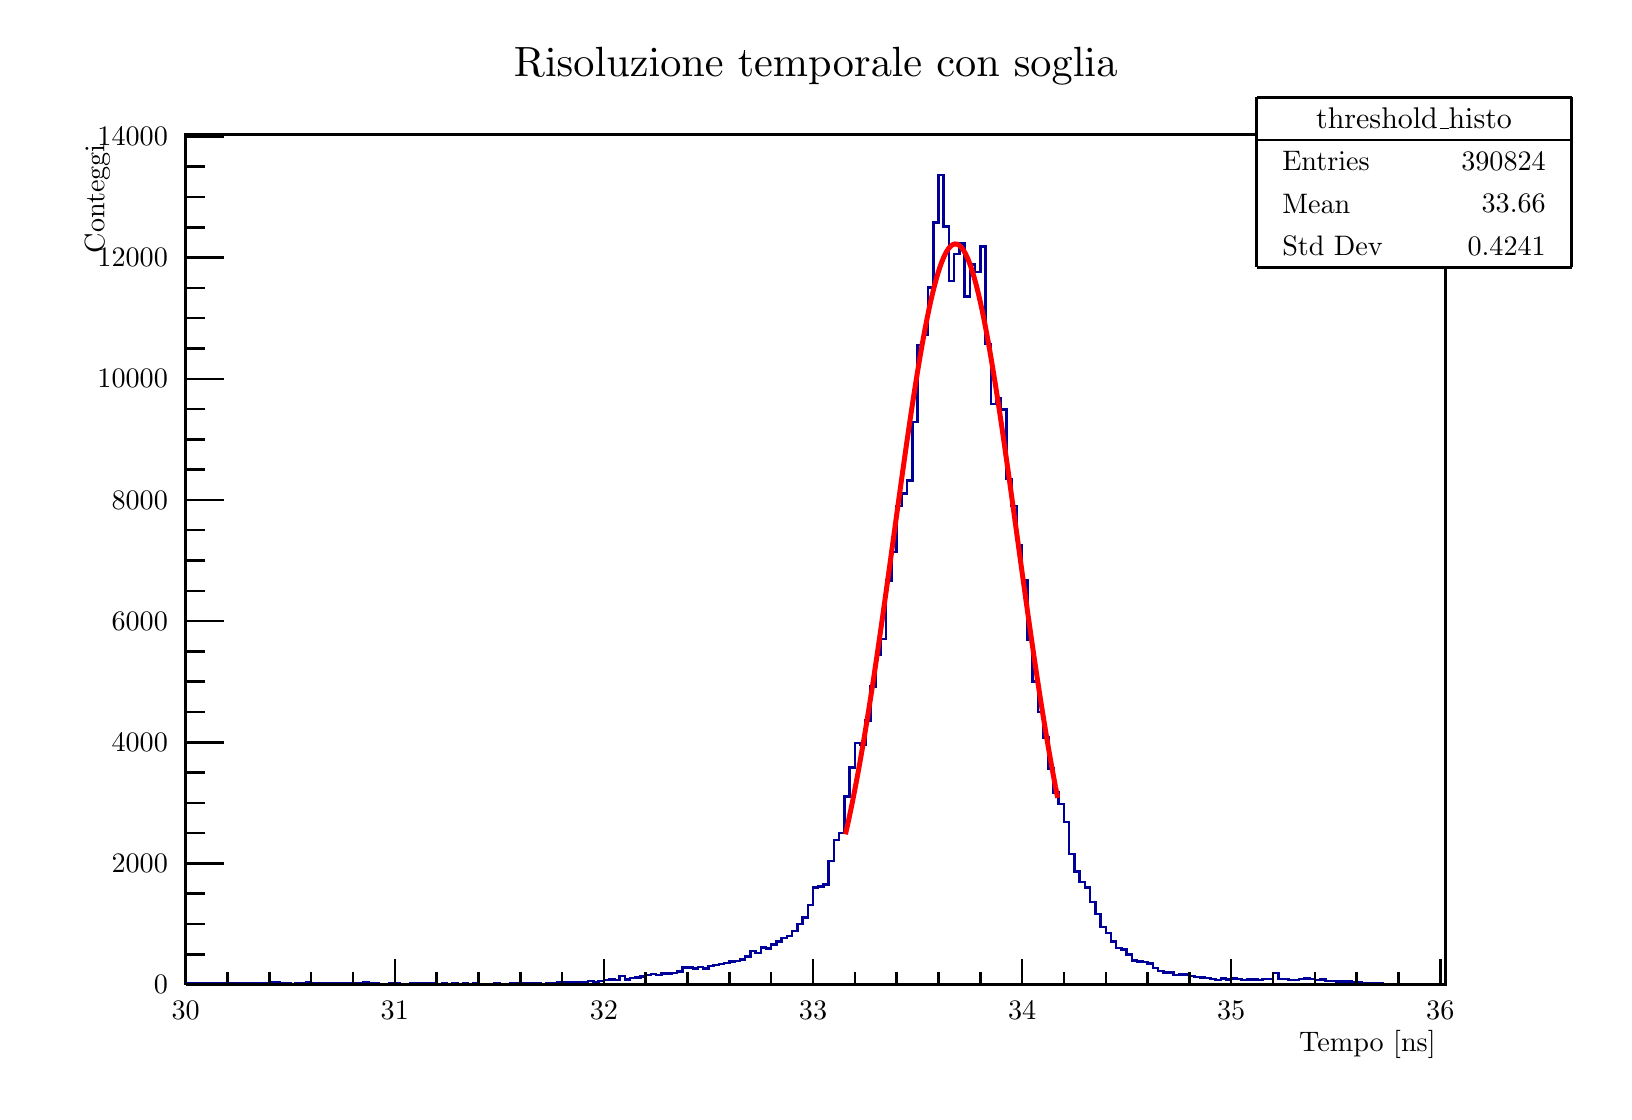
\begin{tikzpicture}
\pgfdeclareplotmark{cross} {
\pgfpathmoveto{\pgfpoint{-0.3\pgfplotmarksize}{\pgfplotmarksize}}
\pgfpathlineto{\pgfpoint{+0.3\pgfplotmarksize}{\pgfplotmarksize}}
\pgfpathlineto{\pgfpoint{+0.3\pgfplotmarksize}{0.3\pgfplotmarksize}}
\pgfpathlineto{\pgfpoint{+1\pgfplotmarksize}{0.3\pgfplotmarksize}}
\pgfpathlineto{\pgfpoint{+1\pgfplotmarksize}{-0.3\pgfplotmarksize}}
\pgfpathlineto{\pgfpoint{+0.3\pgfplotmarksize}{-0.3\pgfplotmarksize}}
\pgfpathlineto{\pgfpoint{+0.3\pgfplotmarksize}{-1.\pgfplotmarksize}}
\pgfpathlineto{\pgfpoint{-0.3\pgfplotmarksize}{-1.\pgfplotmarksize}}
\pgfpathlineto{\pgfpoint{-0.3\pgfplotmarksize}{-0.3\pgfplotmarksize}}
\pgfpathlineto{\pgfpoint{-1.\pgfplotmarksize}{-0.3\pgfplotmarksize}}
\pgfpathlineto{\pgfpoint{-1.\pgfplotmarksize}{0.3\pgfplotmarksize}}
\pgfpathlineto{\pgfpoint{-0.3\pgfplotmarksize}{0.3\pgfplotmarksize}}
\pgfpathclose
\pgfusepathqstroke
}
\pgfdeclareplotmark{cross*} {
\pgfpathmoveto{\pgfpoint{-0.3\pgfplotmarksize}{\pgfplotmarksize}}
\pgfpathlineto{\pgfpoint{+0.3\pgfplotmarksize}{\pgfplotmarksize}}
\pgfpathlineto{\pgfpoint{+0.3\pgfplotmarksize}{0.3\pgfplotmarksize}}
\pgfpathlineto{\pgfpoint{+1\pgfplotmarksize}{0.3\pgfplotmarksize}}
\pgfpathlineto{\pgfpoint{+1\pgfplotmarksize}{-0.3\pgfplotmarksize}}
\pgfpathlineto{\pgfpoint{+0.3\pgfplotmarksize}{-0.3\pgfplotmarksize}}
\pgfpathlineto{\pgfpoint{+0.3\pgfplotmarksize}{-1.\pgfplotmarksize}}
\pgfpathlineto{\pgfpoint{-0.3\pgfplotmarksize}{-1.\pgfplotmarksize}}
\pgfpathlineto{\pgfpoint{-0.3\pgfplotmarksize}{-0.3\pgfplotmarksize}}
\pgfpathlineto{\pgfpoint{-1.\pgfplotmarksize}{-0.3\pgfplotmarksize}}
\pgfpathlineto{\pgfpoint{-1.\pgfplotmarksize}{0.3\pgfplotmarksize}}
\pgfpathlineto{\pgfpoint{-0.3\pgfplotmarksize}{0.3\pgfplotmarksize}}
\pgfpathclose
\pgfusepathqfillstroke
}
\pgfdeclareplotmark{newstar} {
\pgfpathmoveto{\pgfqpoint{0pt}{\pgfplotmarksize}}
\pgfpathlineto{\pgfqpointpolar{44}{0.5\pgfplotmarksize}}
\pgfpathlineto{\pgfqpointpolar{18}{\pgfplotmarksize}}
\pgfpathlineto{\pgfqpointpolar{-20}{0.5\pgfplotmarksize}}
\pgfpathlineto{\pgfqpointpolar{-54}{\pgfplotmarksize}}
\pgfpathlineto{\pgfqpointpolar{-90}{0.5\pgfplotmarksize}}
\pgfpathlineto{\pgfqpointpolar{234}{\pgfplotmarksize}}
\pgfpathlineto{\pgfqpointpolar{198}{0.5\pgfplotmarksize}}
\pgfpathlineto{\pgfqpointpolar{162}{\pgfplotmarksize}}
\pgfpathlineto{\pgfqpointpolar{134}{0.5\pgfplotmarksize}}
\pgfpathclose
\pgfusepathqstroke
}
\pgfdeclareplotmark{newstar*} {
\pgfpathmoveto{\pgfqpoint{0pt}{\pgfplotmarksize}}
\pgfpathlineto{\pgfqpointpolar{44}{0.5\pgfplotmarksize}}
\pgfpathlineto{\pgfqpointpolar{18}{\pgfplotmarksize}}
\pgfpathlineto{\pgfqpointpolar{-20}{0.5\pgfplotmarksize}}
\pgfpathlineto{\pgfqpointpolar{-54}{\pgfplotmarksize}}
\pgfpathlineto{\pgfqpointpolar{-90}{0.5\pgfplotmarksize}}
\pgfpathlineto{\pgfqpointpolar{234}{\pgfplotmarksize}}
\pgfpathlineto{\pgfqpointpolar{198}{0.5\pgfplotmarksize}}
\pgfpathlineto{\pgfqpointpolar{162}{\pgfplotmarksize}}
\pgfpathlineto{\pgfqpointpolar{134}{0.5\pgfplotmarksize}}
\pgfpathclose
\pgfusepathqfillstroke
}
\definecolor{c}{rgb}{1,1,1};
\draw [color=c, fill=c] (0,0) rectangle (20,13.4957);
\draw [color=c, fill=c] (2,1.34957) rectangle (18,12.1461);
\definecolor{c}{rgb}{0,0,0};
\draw [c,line width=0.9] (2,1.34957) -- (2,12.1461) -- (18,12.1461) -- (18,1.34957) -- (2,1.34957);
\definecolor{c}{rgb}{1,1,1};
\draw [color=c, fill=c] (2,1.34957) rectangle (18,12.1461);
\definecolor{c}{rgb}{0,0,0};
\draw [c,line width=0.9] (2,1.34957) -- (2,12.1461) -- (18,12.1461) -- (18,1.34957) -- (2,1.34957);
\definecolor{c}{rgb}{0,0,0.6};
\draw [c,line width=0.9] (2,1.37034) -- (2.06639,1.37034) -- (2.06639,1.36881) -- (2.13278,1.36881) -- (2.13278,1.36342) -- (2.19917,1.36342) -- (2.19917,1.36342) -- (2.26556,1.36342) -- (2.26556,1.36573) -- (2.33195,1.36573) -- (2.33195,1.36342) --
 (2.39834,1.36342) -- (2.39834,1.36419) -- (2.46473,1.36419) -- (2.46473,1.36573) -- (2.53112,1.36573) -- (2.53112,1.36342) -- (2.59751,1.36342) -- (2.59751,1.36958) -- (2.6639,1.36958) -- (2.6639,1.36419) -- (2.73029,1.36419) -- (2.73029,1.36958) --
 (2.79668,1.36958) -- (2.79668,1.36265) -- (2.86307,1.36265) -- (2.86307,1.36881) -- (2.92946,1.36881) -- (2.92946,1.37034) -- (2.99585,1.37034) -- (2.99585,1.36573) -- (3.06224,1.36573) -- (3.06224,1.3765) -- (3.12863,1.3765) -- (3.12863,1.37342) --
 (3.19502,1.37342) -- (3.19502,1.36573) -- (3.26141,1.36573) -- (3.26141,1.36496) -- (3.3278,1.36496) -- (3.3278,1.35957) -- (3.39419,1.35957) -- (3.39419,1.36265) -- (3.46058,1.36265) -- (3.46058,1.36265) -- (3.52697,1.36265) -- (3.52697,1.37419) --
 (3.59336,1.37419) -- (3.59336,1.36573) -- (3.65975,1.36573) -- (3.65975,1.36342) -- (3.72614,1.36342) -- (3.72614,1.3665) -- (3.79253,1.3665) -- (3.79253,1.36958) -- (3.85892,1.36958) -- (3.85892,1.36111) -- (3.92531,1.36111) -- (3.92531,1.36265) --
 (3.9917,1.36265) -- (3.9917,1.36496) -- (4.05809,1.36496) -- (4.05809,1.37111) -- (4.12448,1.37111) -- (4.12448,1.36573) -- (4.19087,1.36573) -- (4.19087,1.36265) -- (4.25726,1.36265) -- (4.25726,1.37496) -- (4.32365,1.37496) -- (4.32365,1.36265) --
 (4.39004,1.36265) -- (4.39004,1.36573) -- (4.45643,1.36573) -- (4.45643,1.36034) -- (4.52282,1.36034) -- (4.52282,1.36034) -- (4.58921,1.36034) -- (4.58921,1.36188) -- (4.6556,1.36188) -- (4.6556,1.36496) -- (4.72199,1.36496) -- (4.72199,1.35957) --
 (4.78838,1.35957) -- (4.78838,1.3565) -- (4.85477,1.3565) -- (4.85477,1.36342) -- (4.92116,1.36342) -- (4.92116,1.36265) -- (4.98755,1.36265) -- (4.98755,1.36342) -- (5.05394,1.36342) -- (5.05394,1.36573) -- (5.12033,1.36573) -- (5.12033,1.36342) --
 (5.18672,1.36342) -- (5.18672,1.3565) -- (5.25311,1.3565) -- (5.25311,1.36265) -- (5.3195,1.36265) -- (5.3195,1.36034) -- (5.38589,1.36034) -- (5.38589,1.36188) -- (5.45228,1.36188) -- (5.45228,1.3588) -- (5.51867,1.3588) -- (5.51867,1.36265) --
 (5.58506,1.36265) -- (5.58506,1.35726) -- (5.65145,1.35726) -- (5.65145,1.36111) -- (5.71784,1.36111) -- (5.71784,1.3588) -- (5.78423,1.3588) -- (5.78423,1.35726) -- (5.85062,1.35726) -- (5.85062,1.36034) -- (5.91701,1.36034) -- (5.91701,1.36573) --
 (5.9834,1.36573) -- (5.9834,1.36034) -- (6.04979,1.36034) -- (6.04979,1.35803) -- (6.11618,1.35803) -- (6.11618,1.36188) -- (6.18257,1.36188) -- (6.18257,1.36188) -- (6.24896,1.36188) -- (6.24896,1.36496) -- (6.31535,1.36496) -- (6.31535,1.36188) --
 (6.38174,1.36188) -- (6.38174,1.36958) -- (6.44813,1.36958) -- (6.44813,1.36188) -- (6.51452,1.36188) -- (6.51452,1.3565) -- (6.58091,1.3565) -- (6.58091,1.36419) -- (6.6473,1.36419) -- (6.6473,1.36573) -- (6.71369,1.36573) -- (6.71369,1.37342) --
 (6.78008,1.37342) -- (6.78008,1.37342) -- (6.84647,1.37342) -- (6.84647,1.38035) -- (6.91286,1.38035) -- (6.91286,1.37496) -- (6.97925,1.37496) -- (6.97925,1.38112) -- (7.04564,1.38112) -- (7.04564,1.38342) -- (7.11203,1.38342) -- (7.11203,1.39727)
 -- (7.17842,1.39727) -- (7.17842,1.38419) -- (7.24481,1.38419) -- (7.24481,1.39497) -- (7.3112,1.39497) -- (7.3112,1.40728) -- (7.37759,1.40728) -- (7.37759,1.41343) -- (7.44398,1.41343) -- (7.44398,1.40574) -- (7.51037,1.40574) -- (7.51037,1.46037)
 -- (7.57676,1.46037) -- (7.57676,1.41497) -- (7.64315,1.41497) -- (7.64315,1.43113) -- (7.70954,1.43113) -- (7.70954,1.44267) -- (7.77593,1.44267) -- (7.77593,1.45498) -- (7.84232,1.45498) -- (7.84232,1.47114) -- (7.90871,1.47114) --
 (7.90871,1.48345) -- (7.9751,1.48345) -- (7.9751,1.47114) -- (8.04149,1.47114) -- (8.04149,1.49268) -- (8.10788,1.49268) -- (8.10788,1.48806) -- (8.17427,1.48806) -- (8.17427,1.49807) -- (8.24066,1.49807) -- (8.24066,1.51576) -- (8.30705,1.51576) --
 (8.30705,1.56424) -- (8.37344,1.56424) -- (8.37344,1.56424) -- (8.43983,1.56424) -- (8.43983,1.5527) -- (8.50622,1.5527) -- (8.50622,1.57193) -- (8.57261,1.57193) -- (8.57261,1.55116) -- (8.639,1.55116) -- (8.639,1.58578) -- (8.70539,1.58578) --
 (8.70539,1.59886) -- (8.77178,1.59886) -- (8.77178,1.61271) -- (8.83817,1.61271) -- (8.83817,1.62502) -- (8.90456,1.62502) -- (8.90456,1.64579) -- (8.97095,1.64579) -- (8.97095,1.65041) -- (9.03734,1.65041) -- (9.03734,1.67119) -- (9.10373,1.67119)
 -- (9.10373,1.70889) -- (9.17012,1.70889) -- (9.17012,1.77813) -- (9.23651,1.77813) -- (9.23651,1.74967) -- (9.3029,1.74967) -- (9.3029,1.82199) -- (9.36929,1.82199) -- (9.36929,1.80891) -- (9.43568,1.80891) -- (9.43568,1.85892) -- (9.50207,1.85892)
 -- (9.50207,1.89431) -- (9.56846,1.89431) -- (9.56846,1.93971) -- (9.63485,1.93971) -- (9.63485,1.96972) -- (9.70124,1.96972) -- (9.70124,2.03281) -- (9.76763,2.03281) -- (9.76763,2.11975) -- (9.83402,2.11975) -- (9.83402,2.20131) --
 (9.90041,2.20131) -- (9.90041,2.3575) -- (9.9668,2.3575) -- (9.9668,2.58448) -- (10.0332,2.58448) -- (10.0332,2.59833) -- (10.0996,2.59833) -- (10.0996,2.62064) -- (10.166,2.62064) -- (10.166,2.92071) -- (10.2324,2.92071) -- (10.2324,3.18616) --
 (10.2988,3.18616) -- (10.2988,3.27541) -- (10.3651,3.27541) -- (10.3651,3.74014) -- (10.4315,3.74014) -- (10.4315,4.10561) -- (10.4979,4.10561) -- (10.4979,4.41491) -- (10.5643,4.41491) -- (10.5643,4.38952) -- (10.6307,4.38952) -- (10.6307,4.70113)
 -- (10.6971,4.70113) -- (10.6971,5.13816) -- (10.7635,5.13816) -- (10.7635,5.53364) -- (10.8299,5.53364) -- (10.8299,5.736) -- (10.8963,5.736) -- (10.8963,6.47925) -- (10.9627,6.47925) -- (10.9627,6.84395) -- (11.029,6.84395) -- (11.029,7.42947) --
 (11.0954,7.42947) -- (11.0954,7.58643) -- (11.1618,7.58643) -- (11.1618,7.75109) -- (11.2282,7.75109) -- (11.2282,8.49665) -- (11.2946,8.49665) -- (11.2946,9.47304) -- (11.361,9.47304) -- (11.361,9.60153) -- (11.4274,9.60153) -- (11.4274,10.2032) --
 (11.4938,10.2032) -- (11.4938,11.0273) -- (11.5602,11.0273) -- (11.5602,11.632) -- (11.6266,11.632) -- (11.6266,10.9749) -- (11.6929,10.9749) -- (11.6929,10.2855) -- (11.7593,10.2855) -- (11.7593,10.6264) -- (11.8257,10.6264) -- (11.8257,10.7603) --
 (11.8921,10.7603) -- (11.8921,10.0878) -- (11.9585,10.0878) -- (11.9585,10.4956) -- (12.0249,10.4956) -- (12.0249,10.3994) -- (12.0913,10.3994) -- (12.0913,10.7264) -- (12.1577,10.7264) -- (12.1577,9.48227) -- (12.2241,9.48227) -- (12.2241,8.7244)
 -- (12.2905,8.7244) -- (12.2905,8.79134) -- (12.3568,8.79134) -- (12.3568,8.6513) -- (12.4232,8.6513) -- (12.4232,7.76955) -- (12.4896,7.76955) -- (12.4896,7.4287) -- (12.556,7.4287) -- (12.556,6.92397) -- (12.6224,6.92397) -- (12.6224,6.48771) --
 (12.6888,6.48771) -- (12.6888,5.73215) -- (12.7552,5.73215) -- (12.7552,5.19971) -- (12.8216,5.19971) -- (12.8216,4.81347) -- (12.888,4.81347) -- (12.888,4.48647) -- (12.9544,4.48647) -- (12.9544,4.09715) -- (13.0207,4.09715) -- (13.0207,3.78707) --
 (13.0871,3.78707) -- (13.0871,3.64319) -- (13.1535,3.64319) -- (13.1535,3.41314) -- (13.2199,3.41314) -- (13.2199,3.00996) -- (13.2863,3.00996) -- (13.2863,2.78299) -- (13.3527,2.78299) -- (13.3527,2.6545) -- (13.4191,2.6545) -- (13.4191,2.58063) --
 (13.4855,2.58063) -- (13.4855,2.40059) -- (13.5519,2.40059) -- (13.5519,2.24363) -- (13.6183,2.24363) -- (13.6183,2.0782) -- (13.6846,2.0782) -- (13.6846,2.00665) -- (13.751,2.00665) -- (13.751,1.89893) -- (13.8174,1.89893) -- (13.8174,1.81276) --
 (13.8838,1.81276) -- (13.8838,1.79275) -- (13.9502,1.79275) -- (13.9502,1.73505) -- (14.0166,1.73505) -- (14.0166,1.65734) -- (14.083,1.65734) -- (14.083,1.64426) -- (14.1494,1.64426) -- (14.1494,1.63964) -- (14.2158,1.63964) -- (14.2158,1.61579) --
 (14.2822,1.61579) -- (14.2822,1.56116) -- (14.3485,1.56116) -- (14.3485,1.52423) -- (14.4149,1.52423) -- (14.4149,1.50038) -- (14.4813,1.50038) -- (14.4813,1.50422) -- (14.5477,1.50422) -- (14.5477,1.47037) -- (14.6141,1.47037) -- (14.6141,1.47575)
 -- (14.6805,1.47575) -- (14.6805,1.47652) -- (14.7469,1.47652) -- (14.7469,1.45575) -- (14.8133,1.45575) -- (14.8133,1.44652) -- (14.8797,1.44652) -- (14.8797,1.44267) -- (14.9461,1.44267) -- (14.9461,1.43498) -- (15.0124,1.43498) --
 (15.0124,1.4219) -- (15.0788,1.4219) -- (15.0788,1.41112) -- (15.1452,1.41112) -- (15.1452,1.42959) -- (15.2116,1.42959) -- (15.2116,1.41343) -- (15.278,1.41343) -- (15.278,1.42497) -- (15.3444,1.42497) -- (15.3444,1.41882) -- (15.4108,1.41882) --
 (15.4108,1.40497) -- (15.4772,1.40497) -- (15.4772,1.41728) -- (15.5436,1.41728) -- (15.5436,1.41343) -- (15.61,1.41343) -- (15.61,1.40728) -- (15.6763,1.40728) -- (15.6763,1.42266) -- (15.7427,1.42266) -- (15.7427,1.42036) -- (15.8091,1.42036) --
 (15.8091,1.49653) -- (15.8755,1.49653) -- (15.8755,1.41805) -- (15.9419,1.41805) -- (15.9419,1.41882) -- (16.0083,1.41882) -- (16.0083,1.40882) -- (16.0747,1.40882) -- (16.0747,1.40728) -- (16.1411,1.40728) -- (16.1411,1.41805) -- (16.2075,1.41805)
 -- (16.2075,1.42959) -- (16.2739,1.42959) -- (16.2739,1.42113) -- (16.3402,1.42113) -- (16.3402,1.40958) -- (16.4066,1.40958) -- (16.4066,1.41189) -- (16.473,1.41189) -- (16.473,1.39804) -- (16.5394,1.39804) -- (16.5394,1.3965) -- (16.6058,1.3965)
 -- (16.6058,1.3865) -- (16.6722,1.3865) -- (16.6722,1.38804) -- (16.7386,1.38804) -- (16.7386,1.39189) -- (16.805,1.39189) -- (16.805,1.37419) -- (16.8714,1.37419) -- (16.8714,1.38342) -- (16.9378,1.38342) -- (16.9378,1.37188) -- (17.0041,1.37188)
 -- (17.0041,1.36573) -- (17.0705,1.36573) -- (17.0705,1.36573) -- (17.1369,1.36573) -- (17.1369,1.36881) -- (17.2033,1.36881) -- (17.2033,1.35803) -- (17.2697,1.35803) -- (17.2697,1.35957) -- (17.3361,1.35957) -- (17.3361,1.35573) --
 (17.4025,1.35573) -- (17.4025,1.3588) -- (17.4689,1.3588) -- (17.4689,1.35496) -- (17.5353,1.35496) -- (17.5353,1.35573) -- (17.6017,1.35573) -- (17.6017,1.35419) -- (17.668,1.35419) -- (17.668,1.35188) -- (17.7344,1.35188) -- (17.7344,1.3565) --
 (17.8008,1.3565) -- (17.8008,1.35342) -- (17.8672,1.35342) -- (17.8672,1.35265) -- (17.9336,1.35265) -- (17.9336,1.35265) -- (18,1.35265);
\definecolor{c}{rgb}{1,1,1};
\draw [color=c, fill=c] (15.6,10.4592) rectangle (19.6,12.6185);
\definecolor{c}{rgb}{0,0,0};
\draw [c,line width=0.9] (15.6,10.4592) -- (19.6,10.4592);
\draw [c,line width=0.9] (19.6,10.4592) -- (19.6,12.6185);
\draw [c,line width=0.9] (19.6,12.6185) -- (15.6,12.6185);
\draw [c,line width=0.9] (15.6,12.6185) -- (15.6,10.4592);
\draw (17.6,12.3486) node[scale=1.08185, color=c, rotate=0]{threshold\_histo};
\draw [c,line width=0.9] (15.6,12.0787) -- (19.6,12.0787);
\draw [anchor= west] (15.8,11.8087) node[scale=1.01821, color=c, rotate=0]{Entries };
\draw [anchor= east] (19.4,11.8087) node[scale=1.01821, color=c, rotate=0]{ 390824};
\draw [anchor= west] (15.8,11.2689) node[scale=1.01821, color=c, rotate=0]{Mean  };
\draw [anchor= east] (19.4,11.2689) node[scale=1.01821, color=c, rotate=0]{  33.66};
\draw [anchor= west] (15.8,10.7291) node[scale=1.01821, color=c, rotate=0]{Std Dev   };
\draw [anchor= east] (19.4,10.7291) node[scale=1.01821, color=c, rotate=0]{ 0.4241};
\definecolor{c}{rgb}{1,0,0};
\draw [c,line width=1.8] (10.3788,3.25793) -- (10.406,3.37912) -- (10.4332,3.50539) -- (10.4604,3.63674) -- (10.4876,3.77316) -- (10.5149,3.9146) -- (10.5421,4.06102) -- (10.5693,4.21231) -- (10.5965,4.36839) -- (10.6237,4.52913) -- (10.651,4.69437)
 -- (10.6782,4.86393) -- (10.7054,5.03762) -- (10.7326,5.21521) -- (10.7598,5.39644) -- (10.7871,5.58104) -- (10.8143,5.7687) -- (10.8415,5.9591) -- (10.8687,6.15187) -- (10.8959,6.34665) -- (10.9232,6.54303) -- (10.9504,6.7406) -- (10.9776,6.9389)
 -- (11.0048,7.13748) -- (11.032,7.33586) -- (11.0593,7.53354) -- (11.0865,7.73001) -- (11.1137,7.92475) -- (11.1409,8.11723) -- (11.1681,8.30691) -- (11.1954,8.49325) -- (11.2226,8.6757) -- (11.2498,8.8537) -- (11.277,9.02672) -- (11.3042,9.19423)
 -- (11.3315,9.35568) -- (11.3587,9.51055) -- (11.3859,9.65835) -- (11.4131,9.79859) -- (11.4403,9.93079) -- (11.4676,10.0545) -- (11.4948,10.1693) -- (11.522,10.2748) -- (11.5492,10.3706) -- (11.5764,10.4564) -- (11.6037,10.5319) --
 (11.6309,10.5968) -- (11.6581,10.6509) -- (11.6853,10.694) -- (11.7125,10.7259);
\draw [c,line width=1.8] (11.7125,10.7259) -- (11.7398,10.7465) -- (11.767,10.7558) -- (11.7942,10.7536) -- (11.8214,10.7401) -- (11.8486,10.7153) -- (11.8759,10.6792) -- (11.9031,10.632) -- (11.9303,10.5738) -- (11.9575,10.5049) -- (11.9847,10.4255)
 -- (12.012,10.336) -- (12.0392,10.2365) -- (12.0664,10.1275) -- (12.0936,10.0093) -- (12.1208,9.88236) -- (12.148,9.7471) -- (12.1753,9.60399) -- (12.2025,9.45348) -- (12.2297,9.29609) -- (12.2569,9.13232) -- (12.2841,8.96269) -- (12.3114,8.78774)
 -- (12.3386,8.60801) -- (12.3658,8.42405) -- (12.393,8.2364) -- (12.4202,8.04561) -- (12.4475,7.85222) -- (12.4747,7.65677) -- (12.5019,7.45979) -- (12.5291,7.26179) -- (12.5563,7.06327) -- (12.5836,6.86474) -- (12.6108,6.66666) -- (12.638,6.46949)
 -- (12.6652,6.27366) -- (12.6924,6.07958) -- (12.7197,5.88765) -- (12.7469,5.69824) -- (12.7741,5.51169) -- (12.8013,5.32831) -- (12.8285,5.14841) -- (12.8558,4.97225) -- (12.883,4.80008) -- (12.9102,4.63211) -- (12.9374,4.46853) --
 (12.9646,4.30952) -- (12.9919,4.15521) -- (13.0191,4.00573) -- (13.0463,3.86117);
\draw [c,line width=1.8] (13.0463,3.86117) -- (13.0735,3.72159);
\definecolor{c}{rgb}{0,0,0};
\draw [c,line width=0.9] (2,1.34957) -- (18,1.34957);
\draw [anchor= east] (18,0.593811) node[scale=1.01821, color=c, rotate=0]{Tempo [ns]};
\draw [c,line width=0.9] (2,1.67347) -- (2,1.34957);
\draw [c,line width=0.9] (2.53112,1.51152) -- (2.53112,1.34957);
\draw [c,line width=0.9] (3.06224,1.51152) -- (3.06224,1.34957);
\draw [c,line width=0.9] (3.59336,1.51152) -- (3.59336,1.34957);
\draw [c,line width=0.9] (4.12448,1.51152) -- (4.12448,1.34957);
\draw [c,line width=0.9] (4.6556,1.67347) -- (4.6556,1.34957);
\draw [c,line width=0.9] (5.18672,1.51152) -- (5.18672,1.34957);
\draw [c,line width=0.9] (5.71784,1.51152) -- (5.71784,1.34957);
\draw [c,line width=0.9] (6.24896,1.51152) -- (6.24896,1.34957);
\draw [c,line width=0.9] (6.78008,1.51152) -- (6.78008,1.34957);
\draw [c,line width=0.9] (7.3112,1.67347) -- (7.3112,1.34957);
\draw [c,line width=0.9] (7.84232,1.51152) -- (7.84232,1.34957);
\draw [c,line width=0.9] (8.37344,1.51152) -- (8.37344,1.34957);
\draw [c,line width=0.9] (8.90456,1.51152) -- (8.90456,1.34957);
\draw [c,line width=0.9] (9.43568,1.51152) -- (9.43568,1.34957);
\draw [c,line width=0.9] (9.9668,1.67347) -- (9.9668,1.34957);
\draw [c,line width=0.9] (10.4979,1.51152) -- (10.4979,1.34957);
\draw [c,line width=0.9] (11.029,1.51152) -- (11.029,1.34957);
\draw [c,line width=0.9] (11.5602,1.51152) -- (11.5602,1.34957);
\draw [c,line width=0.9] (12.0913,1.51152) -- (12.0913,1.34957);
\draw [c,line width=0.9] (12.6224,1.67347) -- (12.6224,1.34957);
\draw [c,line width=0.9] (13.1535,1.51152) -- (13.1535,1.34957);
\draw [c,line width=0.9] (13.6846,1.51152) -- (13.6846,1.34957);
\draw [c,line width=0.9] (14.2158,1.51152) -- (14.2158,1.34957);
\draw [c,line width=0.9] (14.7469,1.51152) -- (14.7469,1.34957);
\draw [c,line width=0.9] (15.278,1.67347) -- (15.278,1.34957);
\draw [c,line width=0.9] (15.8091,1.51152) -- (15.8091,1.34957);
\draw [c,line width=0.9] (16.3402,1.51152) -- (16.3402,1.34957);
\draw [c,line width=0.9] (16.8714,1.51152) -- (16.8714,1.34957);
\draw [c,line width=0.9] (17.4025,1.51152) -- (17.4025,1.34957);
\draw [c,line width=0.9] (17.9336,1.67347) -- (17.9336,1.34957);
\draw [c,line width=0.9] (17.9336,1.67347) -- (17.9336,1.34957);
\draw [anchor=base] (2,0.904212) node[scale=1.01821, color=c, rotate=0]{30};
\draw [anchor=base] (4.6556,0.904212) node[scale=1.01821, color=c, rotate=0]{31};
\draw [anchor=base] (7.3112,0.904212) node[scale=1.01821, color=c, rotate=0]{32};
\draw [anchor=base] (9.9668,0.904212) node[scale=1.01821, color=c, rotate=0]{33};
\draw [anchor=base] (12.6224,0.904212) node[scale=1.01821, color=c, rotate=0]{34};
\draw [anchor=base] (15.278,0.904212) node[scale=1.01821, color=c, rotate=0]{35};
\draw [anchor=base] (17.9336,0.904212) node[scale=1.01821, color=c, rotate=0]{36};
\draw [c,line width=0.9] (2,1.34957) -- (2,12.1461);
\draw [anchor= east] (0.88,12.1461) node[scale=1.01821, color=c, rotate=90]{Conteggi};
\draw [c,line width=0.9] (2.48,1.34957) -- (2,1.34957);
\draw [c,line width=0.9] (2.24,1.73428) -- (2,1.73428);
\draw [c,line width=0.9] (2.24,2.11898) -- (2,2.11898);
\draw [c,line width=0.9] (2.24,2.50369) -- (2,2.50369);
\draw [c,line width=0.9] (2.48,2.8884) -- (2,2.8884);
\draw [c,line width=0.9] (2.24,3.2731) -- (2,3.2731);
\draw [c,line width=0.9] (2.24,3.65781) -- (2,3.65781);
\draw [c,line width=0.9] (2.24,4.04252) -- (2,4.04252);
\draw [c,line width=0.9] (2.48,4.42722) -- (2,4.42722);
\draw [c,line width=0.9] (2.24,4.81193) -- (2,4.81193);
\draw [c,line width=0.9] (2.24,5.19664) -- (2,5.19664);
\draw [c,line width=0.9] (2.24,5.58134) -- (2,5.58134);
\draw [c,line width=0.9] (2.48,5.96605) -- (2,5.96605);
\draw [c,line width=0.9] (2.24,6.35076) -- (2,6.35076);
\draw [c,line width=0.9] (2.24,6.73546) -- (2,6.73546);
\draw [c,line width=0.9] (2.24,7.12017) -- (2,7.12017);
\draw [c,line width=0.9] (2.48,7.50488) -- (2,7.50488);
\draw [c,line width=0.9] (2.24,7.88958) -- (2,7.88958);
\draw [c,line width=0.9] (2.24,8.27429) -- (2,8.27429);
\draw [c,line width=0.9] (2.24,8.659) -- (2,8.659);
\draw [c,line width=0.9] (2.48,9.0437) -- (2,9.0437);
\draw [c,line width=0.9] (2.24,9.42841) -- (2,9.42841);
\draw [c,line width=0.9] (2.24,9.81312) -- (2,9.81312);
\draw [c,line width=0.9] (2.24,10.1978) -- (2,10.1978);
\draw [c,line width=0.9] (2.48,10.5825) -- (2,10.5825);
\draw [c,line width=0.9] (2.24,10.9672) -- (2,10.9672);
\draw [c,line width=0.9] (2.24,11.3519) -- (2,11.3519);
\draw [c,line width=0.9] (2.24,11.7366) -- (2,11.7366);
\draw [c,line width=0.9] (2.48,12.1214) -- (2,12.1214);
\draw [c,line width=0.9] (2.48,12.1214) -- (2,12.1214);
\draw [anchor= east] (1.9,1.34957) node[scale=1.01821, color=c, rotate=0]{0};
\draw [anchor= east] (1.9,2.8884) node[scale=1.01821, color=c, rotate=0]{2000};
\draw [anchor= east] (1.9,4.42722) node[scale=1.01821, color=c, rotate=0]{4000};
\draw [anchor= east] (1.9,5.96605) node[scale=1.01821, color=c, rotate=0]{6000};
\draw [anchor= east] (1.9,7.50488) node[scale=1.01821, color=c, rotate=0]{8000};
\draw [anchor= east] (1.9,9.0437) node[scale=1.01821, color=c, rotate=0]{10000};
\draw [anchor= east] (1.9,10.5825) node[scale=1.01821, color=c, rotate=0]{12000};
\draw [anchor= east] (1.9,12.1214) node[scale=1.01821, color=c, rotate=0]{14000};
\definecolor{c}{rgb}{1,1,1};
\draw [color=c, fill=c] (15.6,10.4592) rectangle (19.6,12.6185);
\definecolor{c}{rgb}{0,0,0};
\draw [c,line width=0.9] (15.6,10.4592) -- (19.6,10.4592);
\draw [c,line width=0.9] (19.6,10.4592) -- (19.6,12.6185);
\draw [c,line width=0.9] (19.6,12.6185) -- (15.6,12.6185);
\draw [c,line width=0.9] (15.6,12.6185) -- (15.6,10.4592);
\draw (17.6,12.3486) node[scale=1.08185, color=c, rotate=0]{threshold\_histo};
\draw [c,line width=0.9] (15.6,12.0787) -- (19.6,12.0787);
\draw [anchor= west] (15.8,11.8087) node[scale=1.01821, color=c, rotate=0]{Entries };
\draw [anchor= east] (19.4,11.8087) node[scale=1.01821, color=c, rotate=0]{ 390824};
\draw [anchor= west] (15.8,11.2689) node[scale=1.01821, color=c, rotate=0]{Mean  };
\draw [anchor= east] (19.4,11.2689) node[scale=1.01821, color=c, rotate=0]{  33.66};
\draw [anchor= west] (15.8,10.7291) node[scale=1.01821, color=c, rotate=0]{Std Dev   };
\draw [anchor= east] (19.4,10.7291) node[scale=1.01821, color=c, rotate=0]{ 0.4241};
\draw (10,13.0156) node[scale=1.52731, color=c, rotate=0]{Risoluzione temporale con soglia};
\end{tikzpicture}

%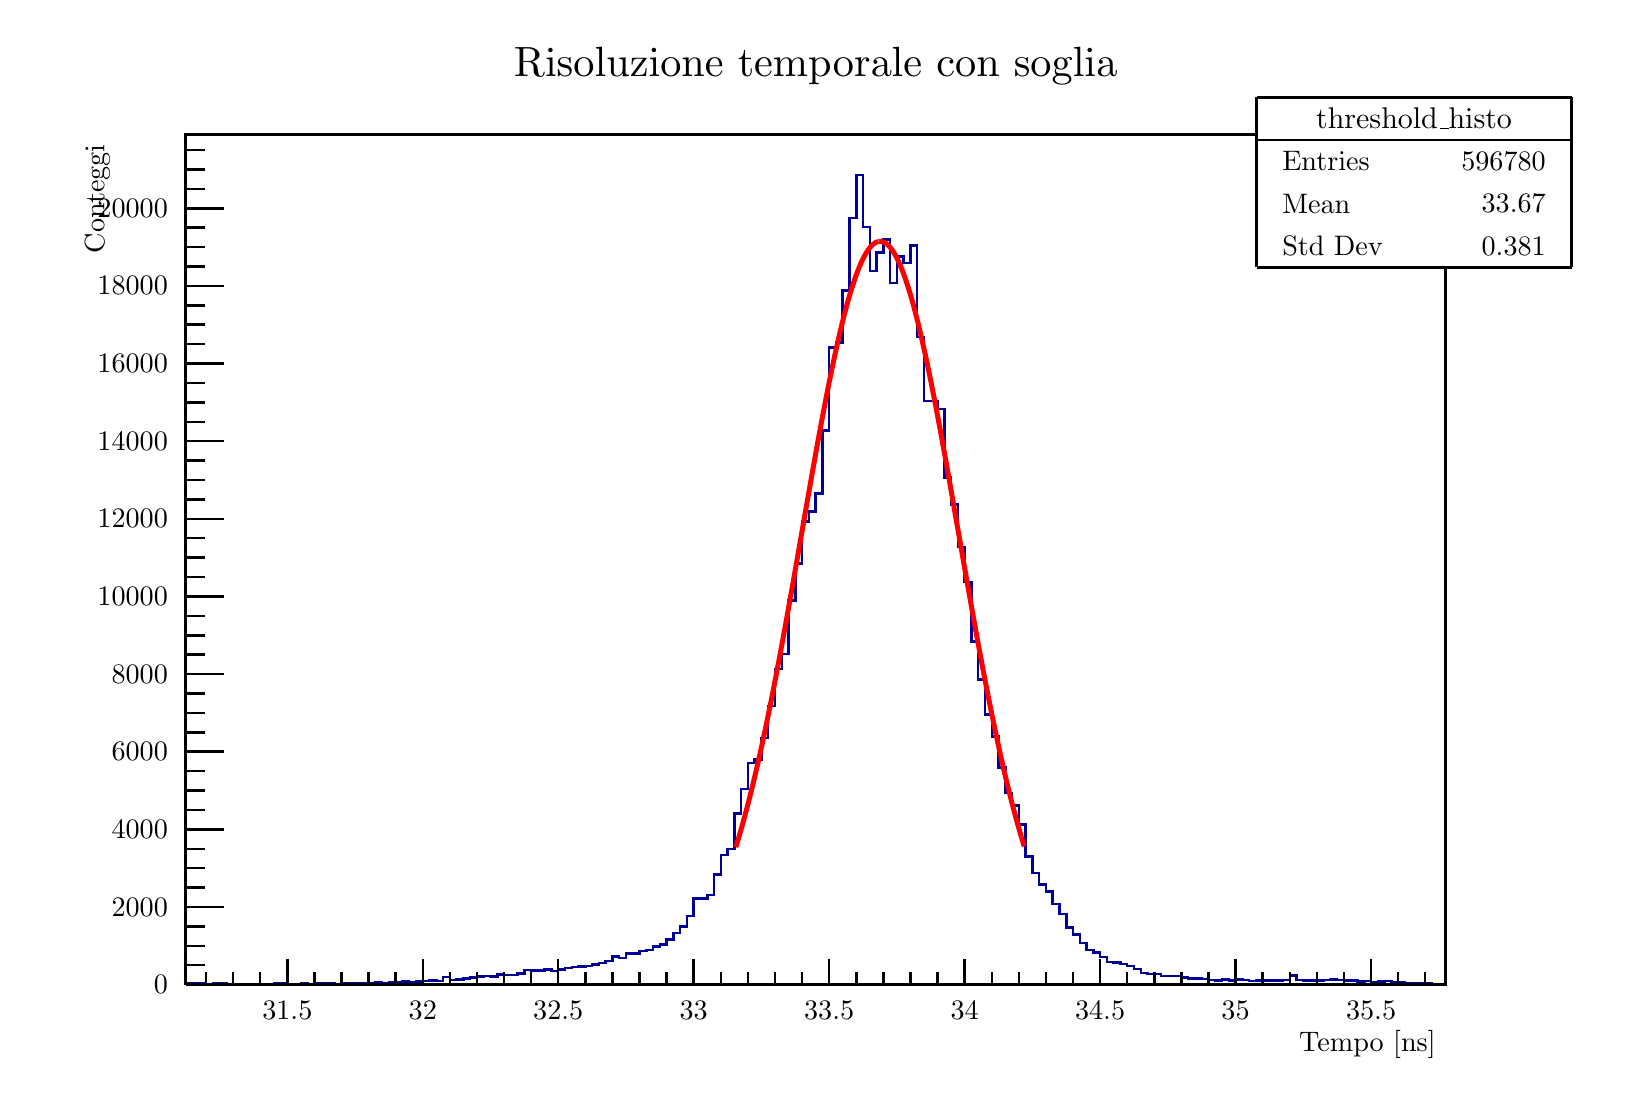
\begin{tikzpicture}
\pgfdeclareplotmark{cross} {
\pgfpathmoveto{\pgfpoint{-0.3\pgfplotmarksize}{\pgfplotmarksize}}
\pgfpathlineto{\pgfpoint{+0.3\pgfplotmarksize}{\pgfplotmarksize}}
\pgfpathlineto{\pgfpoint{+0.3\pgfplotmarksize}{0.3\pgfplotmarksize}}
\pgfpathlineto{\pgfpoint{+1\pgfplotmarksize}{0.3\pgfplotmarksize}}
\pgfpathlineto{\pgfpoint{+1\pgfplotmarksize}{-0.3\pgfplotmarksize}}
\pgfpathlineto{\pgfpoint{+0.3\pgfplotmarksize}{-0.3\pgfplotmarksize}}
\pgfpathlineto{\pgfpoint{+0.3\pgfplotmarksize}{-1.\pgfplotmarksize}}
\pgfpathlineto{\pgfpoint{-0.3\pgfplotmarksize}{-1.\pgfplotmarksize}}
\pgfpathlineto{\pgfpoint{-0.3\pgfplotmarksize}{-0.3\pgfplotmarksize}}
\pgfpathlineto{\pgfpoint{-1.\pgfplotmarksize}{-0.3\pgfplotmarksize}}
\pgfpathlineto{\pgfpoint{-1.\pgfplotmarksize}{0.3\pgfplotmarksize}}
\pgfpathlineto{\pgfpoint{-0.3\pgfplotmarksize}{0.3\pgfplotmarksize}}
\pgfpathclose
\pgfusepathqstroke
}
\pgfdeclareplotmark{cross*} {
\pgfpathmoveto{\pgfpoint{-0.3\pgfplotmarksize}{\pgfplotmarksize}}
\pgfpathlineto{\pgfpoint{+0.3\pgfplotmarksize}{\pgfplotmarksize}}
\pgfpathlineto{\pgfpoint{+0.3\pgfplotmarksize}{0.3\pgfplotmarksize}}
\pgfpathlineto{\pgfpoint{+1\pgfplotmarksize}{0.3\pgfplotmarksize}}
\pgfpathlineto{\pgfpoint{+1\pgfplotmarksize}{-0.3\pgfplotmarksize}}
\pgfpathlineto{\pgfpoint{+0.3\pgfplotmarksize}{-0.3\pgfplotmarksize}}
\pgfpathlineto{\pgfpoint{+0.3\pgfplotmarksize}{-1.\pgfplotmarksize}}
\pgfpathlineto{\pgfpoint{-0.3\pgfplotmarksize}{-1.\pgfplotmarksize}}
\pgfpathlineto{\pgfpoint{-0.3\pgfplotmarksize}{-0.3\pgfplotmarksize}}
\pgfpathlineto{\pgfpoint{-1.\pgfplotmarksize}{-0.3\pgfplotmarksize}}
\pgfpathlineto{\pgfpoint{-1.\pgfplotmarksize}{0.3\pgfplotmarksize}}
\pgfpathlineto{\pgfpoint{-0.3\pgfplotmarksize}{0.3\pgfplotmarksize}}
\pgfpathclose
\pgfusepathqfillstroke
}
\pgfdeclareplotmark{newstar} {
\pgfpathmoveto{\pgfqpoint{0pt}{\pgfplotmarksize}}
\pgfpathlineto{\pgfqpointpolar{44}{0.5\pgfplotmarksize}}
\pgfpathlineto{\pgfqpointpolar{18}{\pgfplotmarksize}}
\pgfpathlineto{\pgfqpointpolar{-20}{0.5\pgfplotmarksize}}
\pgfpathlineto{\pgfqpointpolar{-54}{\pgfplotmarksize}}
\pgfpathlineto{\pgfqpointpolar{-90}{0.5\pgfplotmarksize}}
\pgfpathlineto{\pgfqpointpolar{234}{\pgfplotmarksize}}
\pgfpathlineto{\pgfqpointpolar{198}{0.5\pgfplotmarksize}}
\pgfpathlineto{\pgfqpointpolar{162}{\pgfplotmarksize}}
\pgfpathlineto{\pgfqpointpolar{134}{0.5\pgfplotmarksize}}
\pgfpathclose
\pgfusepathqstroke
}
\pgfdeclareplotmark{newstar*} {
\pgfpathmoveto{\pgfqpoint{0pt}{\pgfplotmarksize}}
\pgfpathlineto{\pgfqpointpolar{44}{0.5\pgfplotmarksize}}
\pgfpathlineto{\pgfqpointpolar{18}{\pgfplotmarksize}}
\pgfpathlineto{\pgfqpointpolar{-20}{0.5\pgfplotmarksize}}
\pgfpathlineto{\pgfqpointpolar{-54}{\pgfplotmarksize}}
\pgfpathlineto{\pgfqpointpolar{-90}{0.5\pgfplotmarksize}}
\pgfpathlineto{\pgfqpointpolar{234}{\pgfplotmarksize}}
\pgfpathlineto{\pgfqpointpolar{198}{0.5\pgfplotmarksize}}
\pgfpathlineto{\pgfqpointpolar{162}{\pgfplotmarksize}}
\pgfpathlineto{\pgfqpointpolar{134}{0.5\pgfplotmarksize}}
\pgfpathclose
\pgfusepathqfillstroke
}
\definecolor{c}{rgb}{1,1,1};
\draw [color=c, fill=c] (0,0) rectangle (20,13.4957);
\draw [color=c, fill=c] (2,1.34957) rectangle (18,12.1461);
\definecolor{c}{rgb}{0,0,0};
\draw [c,line width=0.9] (2,1.34957) -- (2,12.1461) -- (18,12.1461) -- (18,1.34957) -- (2,1.34957);
\definecolor{c}{rgb}{1,1,1};
\draw [color=c, fill=c] (2,1.34957) rectangle (18,12.1461);
\definecolor{c}{rgb}{0,0,0};
\draw [c,line width=0.9] (2,1.34957) -- (2,12.1461) -- (18,12.1461) -- (18,1.34957) -- (2,1.34957);
\definecolor{c}{rgb}{0,0,0.6};
\draw [c,line width=0.9] (2,1.3614) -- (2.08602,1.3614) -- (2.08602,1.36436) -- (2.17204,1.36436) -- (2.17204,1.36387) -- (2.25806,1.36387) -- (2.25806,1.35795) -- (2.34409,1.35795) -- (2.34409,1.36189) -- (2.43011,1.36189) -- (2.43011,1.36189) --
 (2.51613,1.36189) -- (2.51613,1.36042) -- (2.60215,1.36042) -- (2.60215,1.35943) -- (2.68817,1.35943) -- (2.68817,1.36042) -- (2.77419,1.36042) -- (2.77419,1.35647) -- (2.86022,1.35647) -- (2.86022,1.36042) -- (2.94624,1.36042) -- (2.94624,1.35992)
 -- (3.03226,1.35992) -- (3.03226,1.35746) -- (3.11828,1.35746) -- (3.11828,1.36189) -- (3.2043,1.36189) -- (3.2043,1.36436) -- (3.29032,1.36436) -- (3.29032,1.35795) -- (3.37634,1.35795) -- (3.37634,1.35598) -- (3.46237,1.35598) -- (3.46237,1.36091)
 -- (3.54839,1.36091) -- (3.54839,1.35844) -- (3.63441,1.35844) -- (3.63441,1.36189) -- (3.72043,1.36189) -- (3.72043,1.36091) -- (3.80645,1.36091) -- (3.80645,1.36485) -- (3.89247,1.36485) -- (3.89247,1.35992) -- (3.97849,1.35992) --
 (3.97849,1.36091) -- (4.06452,1.36091) -- (4.06452,1.36189) -- (4.15054,1.36189) -- (4.15054,1.36288) -- (4.23656,1.36288) -- (4.23656,1.3688) -- (4.32258,1.3688) -- (4.32258,1.36781) -- (4.4086,1.36781) -- (4.4086,1.37619) -- (4.49462,1.37619) --
 (4.49462,1.37077) -- (4.58065,1.37077) -- (4.58065,1.37471) -- (4.66667,1.37471) -- (4.66667,1.37619) -- (4.75269,1.37619) -- (4.75269,1.38852) -- (4.83871,1.38852) -- (4.83871,1.38013) -- (4.92473,1.38013) -- (4.92473,1.38753) -- (5.01075,1.38753)
 -- (5.01075,1.39591) -- (5.09677,1.39591) -- (5.09677,1.40183) -- (5.1828,1.40183) -- (5.1828,1.39443) -- (5.26882,1.39443) -- (5.26882,1.44866) -- (5.35484,1.44866) -- (5.35484,1.40676) -- (5.44086,1.40676) -- (5.44086,1.41514) -- (5.52688,1.41514)
 -- (5.52688,1.4245) -- (5.6129,1.4245) -- (5.6129,1.44126) -- (5.69893,1.44126) -- (5.69893,1.45014) -- (5.78495,1.45014) -- (5.78495,1.46098) -- (5.87097,1.46098) -- (5.87097,1.45359) -- (5.95699,1.45359) -- (5.95699,1.47528) -- (6.04301,1.47528)
 -- (6.04301,1.47183) -- (6.12903,1.47183) -- (6.12903,1.47035) -- (6.21505,1.47035) -- (6.21505,1.48908) -- (6.30108,1.48908) -- (6.30108,1.53197) -- (6.3871,1.53197) -- (6.3871,1.53148) -- (6.47312,1.53148) -- (6.47312,1.52605) -- (6.55914,1.52605)
 -- (6.55914,1.53937) -- (6.64516,1.53937) -- (6.64516,1.52556) -- (6.73118,1.52556) -- (6.73118,1.54331) -- (6.8172,1.54331) -- (6.8172,1.56352) -- (6.90323,1.56352) -- (6.90323,1.57486) -- (6.98925,1.57486) -- (6.98925,1.57732) -- (7.07527,1.57732)
 -- (7.07527,1.58669) -- (7.16129,1.58669) -- (7.16129,1.6069) -- (7.24731,1.6069) -- (7.24731,1.62366) -- (7.33333,1.62366) -- (7.33333,1.65226) -- (7.41935,1.65226) -- (7.41935,1.70648) -- (7.50538,1.70648) -- (7.50538,1.68923) -- (7.5914,1.68923)
 -- (7.5914,1.74198) -- (7.67742,1.74198) -- (7.67742,1.74543) -- (7.76344,1.74543) -- (7.76344,1.77599) -- (7.84946,1.77599) -- (7.84946,1.79226) -- (7.93548,1.79226) -- (7.93548,1.83121) -- (8.02151,1.83121) -- (8.02151,1.85832) --
 (8.10753,1.85832) -- (8.10753,1.91945) -- (8.19355,1.91945) -- (8.19355,2.00473) -- (8.27957,2.00473) -- (8.27957,2.08558) -- (8.36559,2.08558) -- (8.36559,2.22164) -- (8.45161,2.22164) -- (8.45161,2.44052) -- (8.53763,2.44052) -- (8.53763,2.44397)
 -- (8.62366,2.44397) -- (8.62366,2.48785) -- (8.70968,2.48785) -- (8.70968,2.74912) -- (8.7957,2.74912) -- (8.7957,2.99364) -- (8.88172,2.99364) -- (8.88172,3.07153) -- (8.96774,3.07153) -- (8.96774,3.52112) -- (9.05376,3.52112) -- (9.05376,3.83514)
 -- (9.13978,3.83514) -- (9.13978,4.16346) -- (9.22581,4.16346) -- (9.22581,4.20783) -- (9.31183,4.20783) -- (9.31183,4.48143) -- (9.39785,4.48143) -- (9.39785,4.88961) -- (9.48387,4.88961) -- (9.48387,5.35794) -- (9.56989,5.35794) --
 (9.56989,5.54527) -- (9.65591,5.54527) -- (9.65591,6.22606) -- (9.74194,6.22606) -- (9.74194,6.69735) -- (9.82796,6.69735) -- (9.82796,7.22877) -- (9.91398,7.22877) -- (9.91398,7.3599) -- (10,7.3599) -- (10,7.58371) -- (10.086,7.58371) --
 (10.086,8.38726) -- (10.172,8.38726) -- (10.172,9.44321) -- (10.2581,9.44321) -- (10.2581,9.50138) -- (10.3441,9.50138) -- (10.3441,10.1654) -- (10.4301,10.1654) -- (10.4301,11.0863) -- (10.5161,11.0863) -- (10.5161,11.632) -- (10.6022,11.632) --
 (10.6022,10.9724) -- (10.6882,10.9724) -- (10.6882,10.4139) -- (10.7742,10.4139) -- (10.7742,10.649) -- (10.8602,10.649) -- (10.8602,10.8102) -- (10.9462,10.8102) -- (10.9462,10.2576) -- (11.0323,10.2576) -- (11.0323,10.5968) -- (11.1183,10.5968) --
 (11.1183,10.5164) -- (11.2043,10.5164) -- (11.2043,10.7392) -- (11.2903,10.7392) -- (11.2903,9.57582) -- (11.3763,9.57582) -- (11.3763,8.7629) -- (11.4624,8.7629) -- (11.4624,8.75847) -- (11.5484,8.75847) -- (11.5484,8.65889) -- (11.6344,8.65889) --
 (11.6344,7.7878) -- (11.7204,7.7878) -- (11.7204,7.44519) -- (11.8065,7.44519) -- (11.8065,6.90834) -- (11.8925,6.90834) -- (11.8925,6.45973) -- (11.9785,6.45973) -- (11.9785,5.70943) -- (12.0645,5.70943) -- (12.0645,5.22681) -- (12.1505,5.22681) --
 (12.1505,4.77721) -- (12.2366,4.77721) -- (12.2366,4.50263) -- (12.3226,4.50263) -- (12.3226,4.10677) -- (12.4086,4.10677) -- (12.4086,3.78437) -- (12.4946,3.78437) -- (12.4946,3.62711) -- (12.5806,3.62711) -- (12.5806,3.3821) -- (12.6667,3.3821) --
 (12.6667,2.97688) -- (12.7527,2.97688) -- (12.7527,2.7644) -- (12.8387,2.7644) -- (12.8387,2.61848) -- (12.9247,2.61848) -- (12.9247,2.53517) -- (13.0108,2.53517) -- (13.0108,2.37249) -- (13.0968,2.37249) -- (13.0968,2.2453) -- (13.1828,2.2453) --
 (13.1828,2.07227) -- (13.2688,2.07227) -- (13.2688,1.98403) -- (13.3548,1.98403) -- (13.3548,1.881) -- (13.4409,1.881) -- (13.4409,1.79029) -- (13.5269,1.79029) -- (13.5269,1.75726) -- (13.6129,1.75726) -- (13.6129,1.70254) -- (13.6989,1.70254) --
 (13.6989,1.63944) -- (13.7849,1.63944) -- (13.7849,1.63254) -- (13.871,1.63254) -- (13.871,1.61085) -- (13.957,1.61085) -- (13.957,1.58718) -- (14.043,1.58718) -- (14.043,1.54528) -- (14.129,1.54528) -- (14.129,1.49993) -- (14.2151,1.49993) --
 (14.2151,1.48415) -- (14.3011,1.48415) -- (14.3011,1.4876) -- (14.3871,1.4876) -- (14.3871,1.45655) -- (14.4731,1.45655) -- (14.4731,1.46) -- (14.5591,1.46) -- (14.5591,1.45802) -- (14.6452,1.45802) -- (14.6452,1.44126) -- (14.7312,1.44126) --
 (14.7312,1.42549) -- (14.8172,1.42549) -- (14.8172,1.42549) -- (14.9032,1.42549) -- (14.9032,1.42401) -- (14.9892,1.42401) -- (14.9892,1.41021) -- (15.0753,1.41021) -- (15.0753,1.40429) -- (15.1613,1.40429) -- (15.1613,1.41218) -- (15.2473,1.41218)
 -- (15.2473,1.40281) -- (15.3333,1.40281) -- (15.3333,1.41514) -- (15.4194,1.41514) -- (15.4194,1.40577) -- (15.5054,1.40577) -- (15.5054,1.39739) -- (15.5914,1.39739) -- (15.5914,1.4038) -- (15.6774,1.4038) -- (15.6774,1.39887) -- (15.7634,1.39887)
 -- (15.7634,1.39936) -- (15.8495,1.39936) -- (15.8495,1.4038) -- (15.9355,1.4038) -- (15.9355,1.40971) -- (16.0215,1.40971) -- (16.0215,1.4664) -- (16.1075,1.4664) -- (16.1075,1.40774) -- (16.1935,1.40774) -- (16.1935,1.40429) -- (16.2796,1.40429)
 -- (16.2796,1.40478) -- (16.3656,1.40478) -- (16.3656,1.40281) -- (16.4516,1.40281) -- (16.4516,1.40873) -- (16.5376,1.40873) -- (16.5376,1.41464) -- (16.6237,1.41464) -- (16.6237,1.40676) -- (16.7097,1.40676) -- (16.7097,1.40183) --
 (16.7957,1.40183) -- (16.7957,1.4038) -- (16.8817,1.4038) -- (16.8817,1.39197) -- (16.9677,1.39197) -- (16.9677,1.39344) -- (17.0538,1.39344) -- (17.0538,1.38457) -- (17.1398,1.38457) -- (17.1398,1.38852) -- (17.2258,1.38852) -- (17.2258,1.39295) --
 (17.3118,1.39295) -- (17.3118,1.3752) -- (17.3979,1.3752) -- (17.3979,1.38161) -- (17.4839,1.38161) -- (17.4839,1.37126) -- (17.5699,1.37126) -- (17.5699,1.36732) -- (17.6559,1.36732) -- (17.6559,1.36288) -- (17.7419,1.36288) -- (17.7419,1.36337) --
 (17.828,1.36337) -- (17.828,1.35894) -- (17.914,1.35894) -- (17.914,1.35894) -- (18,1.35894);
\definecolor{c}{rgb}{1,1,1};
\draw [color=c, fill=c] (15.6,10.4592) rectangle (19.6,12.6185);
\definecolor{c}{rgb}{0,0,0};
\draw [c,line width=0.9] (15.6,10.4592) -- (19.6,10.4592);
\draw [c,line width=0.9] (19.6,10.4592) -- (19.6,12.6185);
\draw [c,line width=0.9] (19.6,12.6185) -- (15.6,12.6185);
\draw [c,line width=0.9] (15.6,12.6185) -- (15.6,10.4592);
\draw (17.6,12.3486) node[scale=1.08185, color=c, rotate=0]{threshold\_histo};
\draw [c,line width=0.9] (15.6,12.0787) -- (19.6,12.0787);
\draw [anchor= west] (15.8,11.8087) node[scale=1.01821, color=c, rotate=0]{Entries };
\draw [anchor= east] (19.4,11.8087) node[scale=1.01821, color=c, rotate=0]{ 596780};
\draw [anchor= west] (15.8,11.2689) node[scale=1.01821, color=c, rotate=0]{Mean  };
\draw [anchor= east] (19.4,11.2689) node[scale=1.01821, color=c, rotate=0]{  33.67};
\draw [anchor= west] (15.8,10.7291) node[scale=1.01821, color=c, rotate=0]{Std Dev   };
\draw [anchor= east] (19.4,10.7291) node[scale=1.01821, color=c, rotate=0]{  0.381};
\definecolor{c}{rgb}{1,0,0};
\draw [c,line width=1.8] (8.98624,3.09489) -- (9.02323,3.21667) -- (9.06021,3.3442) -- (9.0972,3.47752) -- (9.13419,3.61663) -- (9.17118,3.76151) -- (9.20817,3.91213) -- (9.24516,4.0684) -- (9.28215,4.23025) -- (9.31914,4.39753) -- (9.35613,4.5701)
 -- (9.39312,4.74776) -- (9.43011,4.9303) -- (9.4671,5.11745) -- (9.50409,5.30894) -- (9.54108,5.50444) -- (9.57806,5.7036) -- (9.61505,5.90604) -- (9.65204,6.11134) -- (9.68903,6.31905) -- (9.72602,6.5287) -- (9.76301,6.73976) -- (9.8,6.95173) --
 (9.83699,7.16402) -- (9.87398,7.37607) -- (9.91097,7.58727) -- (9.94796,7.79699) -- (9.98495,8.00461) -- (10.0219,8.20948) -- (10.0589,8.41093) -- (10.0959,8.60831) -- (10.1329,8.80095) -- (10.1699,8.9882) -- (10.2069,9.16938) -- (10.2439,9.34387)
 -- (10.2809,9.51102) -- (10.3178,9.67021) -- (10.3548,9.82085) -- (10.3918,9.96236) -- (10.4288,10.0942) -- (10.4658,10.2159) -- (10.5028,10.3269) -- (10.5398,10.4268) -- (10.5768,10.5152) -- (10.6138,10.5917) -- (10.6508,10.6561) --
 (10.6877,10.708) -- (10.7247,10.7473) -- (10.7617,10.7738) -- (10.7987,10.7874);
\draw [c,line width=1.8] (10.7987,10.7874) -- (10.8357,10.788) -- (10.8727,10.7756) -- (10.9097,10.7503) -- (10.9467,10.7122) -- (10.9837,10.6615) -- (11.0206,10.5983) -- (11.0576,10.5229) -- (11.0946,10.4356) -- (11.1316,10.3367) --
 (11.1686,10.2268) -- (11.2056,10.1061) -- (11.2426,9.97518) -- (11.2796,9.83456) -- (11.3166,9.68475) -- (11.3535,9.52634) -- (11.3905,9.35992) -- (11.4275,9.1861) -- (11.4645,9.00551) -- (11.5015,8.81881) -- (11.5385,8.62665) -- (11.5755,8.42968)
 -- (11.6125,8.22859) -- (11.6495,8.02401) -- (11.6865,7.81663) -- (11.7234,7.60707) -- (11.7604,7.39599) -- (11.7974,7.18399) -- (11.8344,6.9717) -- (11.8714,6.75968) -- (11.9084,6.5485) -- (11.9454,6.3387) -- (11.9824,6.13079) -- (12.0194,5.92524)
 -- (12.0563,5.72252) -- (12.0933,5.52303) -- (12.1303,5.32717) -- (12.1673,5.13529) -- (12.2043,4.94771) -- (12.2413,4.76473) -- (12.2783,4.5866) -- (12.3153,4.41355) -- (12.3523,4.24576) -- (12.3892,4.0834) -- (12.4262,3.92659) -- (12.4632,3.77544)
 -- (12.5002,3.63001) -- (12.5372,3.49036) -- (12.5742,3.3565) -- (12.6112,3.22842);
\draw [c,line width=1.8] (12.6112,3.22842) -- (12.6482,3.1061);
\definecolor{c}{rgb}{0,0,0};
\draw [c,line width=0.9] (2,1.34957) -- (18,1.34957);
\draw [anchor= east] (18,0.593811) node[scale=1.01821, color=c, rotate=0]{Tempo [ns]};
\draw [c,line width=0.9] (3.29032,1.67347) -- (3.29032,1.34957);
\draw [c,line width=0.9] (3.63441,1.51152) -- (3.63441,1.34957);
\draw [c,line width=0.9] (3.97849,1.51152) -- (3.97849,1.34957);
\draw [c,line width=0.9] (4.32258,1.51152) -- (4.32258,1.34957);
\draw [c,line width=0.9] (4.66667,1.51152) -- (4.66667,1.34957);
\draw [c,line width=0.9] (5.01075,1.67347) -- (5.01075,1.34957);
\draw [c,line width=0.9] (5.35484,1.51152) -- (5.35484,1.34957);
\draw [c,line width=0.9] (5.69893,1.51152) -- (5.69893,1.34957);
\draw [c,line width=0.9] (6.04301,1.51152) -- (6.04301,1.34957);
\draw [c,line width=0.9] (6.3871,1.51152) -- (6.3871,1.34957);
\draw [c,line width=0.9] (6.73118,1.67347) -- (6.73118,1.34957);
\draw [c,line width=0.9] (7.07527,1.51152) -- (7.07527,1.34957);
\draw [c,line width=0.9] (7.41935,1.51152) -- (7.41935,1.34957);
\draw [c,line width=0.9] (7.76344,1.51152) -- (7.76344,1.34957);
\draw [c,line width=0.9] (8.10753,1.51152) -- (8.10753,1.34957);
\draw [c,line width=0.9] (8.45161,1.67347) -- (8.45161,1.34957);
\draw [c,line width=0.9] (8.7957,1.51152) -- (8.7957,1.34957);
\draw [c,line width=0.9] (9.13978,1.51152) -- (9.13978,1.34957);
\draw [c,line width=0.9] (9.48387,1.51152) -- (9.48387,1.34957);
\draw [c,line width=0.9] (9.82796,1.51152) -- (9.82796,1.34957);
\draw [c,line width=0.9] (10.172,1.67347) -- (10.172,1.34957);
\draw [c,line width=0.9] (10.5161,1.51152) -- (10.5161,1.34957);
\draw [c,line width=0.9] (10.8602,1.51152) -- (10.8602,1.34957);
\draw [c,line width=0.9] (11.2043,1.51152) -- (11.2043,1.34957);
\draw [c,line width=0.9] (11.5484,1.51152) -- (11.5484,1.34957);
\draw [c,line width=0.9] (11.8925,1.67347) -- (11.8925,1.34957);
\draw [c,line width=0.9] (12.2366,1.51152) -- (12.2366,1.34957);
\draw [c,line width=0.9] (12.5806,1.51152) -- (12.5806,1.34957);
\draw [c,line width=0.9] (12.9247,1.51152) -- (12.9247,1.34957);
\draw [c,line width=0.9] (13.2688,1.51152) -- (13.2688,1.34957);
\draw [c,line width=0.9] (13.6129,1.67347) -- (13.6129,1.34957);
\draw [c,line width=0.9] (13.957,1.51152) -- (13.957,1.34957);
\draw [c,line width=0.9] (14.3011,1.51152) -- (14.3011,1.34957);
\draw [c,line width=0.9] (14.6452,1.51152) -- (14.6452,1.34957);
\draw [c,line width=0.9] (14.9892,1.51152) -- (14.9892,1.34957);
\draw [c,line width=0.9] (15.3333,1.67347) -- (15.3333,1.34957);
\draw [c,line width=0.9] (15.6774,1.51152) -- (15.6774,1.34957);
\draw [c,line width=0.9] (16.0215,1.51152) -- (16.0215,1.34957);
\draw [c,line width=0.9] (16.3656,1.51152) -- (16.3656,1.34957);
\draw [c,line width=0.9] (16.7097,1.51152) -- (16.7097,1.34957);
\draw [c,line width=0.9] (17.0538,1.67347) -- (17.0538,1.34957);
\draw [c,line width=0.9] (3.29032,1.67347) -- (3.29032,1.34957);
\draw [c,line width=0.9] (2.94624,1.51152) -- (2.94624,1.34957);
\draw [c,line width=0.9] (2.60215,1.51152) -- (2.60215,1.34957);
\draw [c,line width=0.9] (2.25806,1.51152) -- (2.25806,1.34957);
\draw [c,line width=0.9] (17.0538,1.67347) -- (17.0538,1.34957);
\draw [c,line width=0.9] (17.3979,1.51152) -- (17.3979,1.34957);
\draw [c,line width=0.9] (17.7419,1.51152) -- (17.7419,1.34957);
\draw [anchor=base] (3.29032,0.904212) node[scale=1.01821, color=c, rotate=0]{31.5};
\draw [anchor=base] (5.01075,0.904212) node[scale=1.01821, color=c, rotate=0]{32};
\draw [anchor=base] (6.73118,0.904212) node[scale=1.01821, color=c, rotate=0]{32.5};
\draw [anchor=base] (8.45161,0.904212) node[scale=1.01821, color=c, rotate=0]{33};
\draw [anchor=base] (10.172,0.904212) node[scale=1.01821, color=c, rotate=0]{33.5};
\draw [anchor=base] (11.8925,0.904212) node[scale=1.01821, color=c, rotate=0]{34};
\draw [anchor=base] (13.6129,0.904212) node[scale=1.01821, color=c, rotate=0]{34.5};
\draw [anchor=base] (15.3333,0.904212) node[scale=1.01821, color=c, rotate=0]{35};
\draw [anchor=base] (17.0538,0.904212) node[scale=1.01821, color=c, rotate=0]{35.5};
\draw [c,line width=0.9] (2,1.34957) -- (2,12.1461);
\draw [anchor= east] (0.88,12.1461) node[scale=1.01821, color=c, rotate=90]{Conteggi};
\draw [c,line width=0.9] (2.48,1.34957) -- (2,1.34957);
\draw [c,line width=0.9] (2.24,1.59606) -- (2,1.59606);
\draw [c,line width=0.9] (2.24,1.84254) -- (2,1.84254);
\draw [c,line width=0.9] (2.24,2.08903) -- (2,2.08903);
\draw [c,line width=0.9] (2.48,2.33552) -- (2,2.33552);
\draw [c,line width=0.9] (2.24,2.582) -- (2,2.582);
\draw [c,line width=0.9] (2.24,2.82849) -- (2,2.82849);
\draw [c,line width=0.9] (2.24,3.07498) -- (2,3.07498);
\draw [c,line width=0.9] (2.48,3.32146) -- (2,3.32146);
\draw [c,line width=0.9] (2.24,3.56795) -- (2,3.56795);
\draw [c,line width=0.9] (2.24,3.81444) -- (2,3.81444);
\draw [c,line width=0.9] (2.24,4.06092) -- (2,4.06092);
\draw [c,line width=0.9] (2.48,4.30741) -- (2,4.30741);
\draw [c,line width=0.9] (2.24,4.5539) -- (2,4.5539);
\draw [c,line width=0.9] (2.24,4.80038) -- (2,4.80038);
\draw [c,line width=0.9] (2.24,5.04687) -- (2,5.04687);
\draw [c,line width=0.9] (2.48,5.29336) -- (2,5.29336);
\draw [c,line width=0.9] (2.24,5.53984) -- (2,5.53984);
\draw [c,line width=0.9] (2.24,5.78633) -- (2,5.78633);
\draw [c,line width=0.9] (2.24,6.03282) -- (2,6.03282);
\draw [c,line width=0.9] (2.48,6.2793) -- (2,6.2793);
\draw [c,line width=0.9] (2.24,6.52579) -- (2,6.52579);
\draw [c,line width=0.9] (2.24,6.77228) -- (2,6.77228);
\draw [c,line width=0.9] (2.24,7.01876) -- (2,7.01876);
\draw [c,line width=0.9] (2.48,7.26525) -- (2,7.26525);
\draw [c,line width=0.9] (2.24,7.51174) -- (2,7.51174);
\draw [c,line width=0.9] (2.24,7.75822) -- (2,7.75822);
\draw [c,line width=0.9] (2.24,8.00471) -- (2,8.00471);
\draw [c,line width=0.9] (2.48,8.2512) -- (2,8.2512);
\draw [c,line width=0.9] (2.24,8.49768) -- (2,8.49768);
\draw [c,line width=0.9] (2.24,8.74417) -- (2,8.74417);
\draw [c,line width=0.9] (2.24,8.99066) -- (2,8.99066);
\draw [c,line width=0.9] (2.48,9.23714) -- (2,9.23714);
\draw [c,line width=0.9] (2.24,9.48363) -- (2,9.48363);
\draw [c,line width=0.9] (2.24,9.73012) -- (2,9.73012);
\draw [c,line width=0.9] (2.24,9.9766) -- (2,9.9766);
\draw [c,line width=0.9] (2.48,10.2231) -- (2,10.2231);
\draw [c,line width=0.9] (2.24,10.4696) -- (2,10.4696);
\draw [c,line width=0.9] (2.24,10.7161) -- (2,10.7161);
\draw [c,line width=0.9] (2.24,10.9626) -- (2,10.9626);
\draw [c,line width=0.9] (2.48,11.209) -- (2,11.209);
\draw [c,line width=0.9] (2.48,11.209) -- (2,11.209);
\draw [c,line width=0.9] (2.24,11.4555) -- (2,11.4555);
\draw [c,line width=0.9] (2.24,11.702) -- (2,11.702);
\draw [c,line width=0.9] (2.24,11.9485) -- (2,11.9485);
\draw [anchor= east] (1.9,1.34957) node[scale=1.01821, color=c, rotate=0]{0};
\draw [anchor= east] (1.9,2.33552) node[scale=1.01821, color=c, rotate=0]{2000};
\draw [anchor= east] (1.9,3.32146) node[scale=1.01821, color=c, rotate=0]{4000};
\draw [anchor= east] (1.9,4.30741) node[scale=1.01821, color=c, rotate=0]{6000};
\draw [anchor= east] (1.9,5.29336) node[scale=1.01821, color=c, rotate=0]{8000};
\draw [anchor= east] (1.9,6.2793) node[scale=1.01821, color=c, rotate=0]{10000};
\draw [anchor= east] (1.9,7.26525) node[scale=1.01821, color=c, rotate=0]{12000};
\draw [anchor= east] (1.9,8.2512) node[scale=1.01821, color=c, rotate=0]{14000};
\draw [anchor= east] (1.9,9.23714) node[scale=1.01821, color=c, rotate=0]{16000};
\draw [anchor= east] (1.9,10.2231) node[scale=1.01821, color=c, rotate=0]{18000};
\draw [anchor= east] (1.9,11.209) node[scale=1.01821, color=c, rotate=0]{20000};
\definecolor{c}{rgb}{1,1,1};
\draw [color=c, fill=c] (15.6,10.4592) rectangle (19.6,12.6185);
\definecolor{c}{rgb}{0,0,0};
\draw [c,line width=0.9] (15.6,10.4592) -- (19.6,10.4592);
\draw [c,line width=0.9] (19.6,10.4592) -- (19.6,12.6185);
\draw [c,line width=0.9] (19.6,12.6185) -- (15.6,12.6185);
\draw [c,line width=0.9] (15.6,12.6185) -- (15.6,10.4592);
\draw (17.6,12.3486) node[scale=1.08185, color=c, rotate=0]{threshold\_histo};
\draw [c,line width=0.9] (15.6,12.0787) -- (19.6,12.0787);
\draw [anchor= west] (15.8,11.8087) node[scale=1.01821, color=c, rotate=0]{Entries };
\draw [anchor= east] (19.4,11.8087) node[scale=1.01821, color=c, rotate=0]{ 596780};
\draw [anchor= west] (15.8,11.2689) node[scale=1.01821, color=c, rotate=0]{Mean  };
\draw [anchor= east] (19.4,11.2689) node[scale=1.01821, color=c, rotate=0]{  33.67};
\draw [anchor= west] (15.8,10.7291) node[scale=1.01821, color=c, rotate=0]{Std Dev   };
\draw [anchor= east] (19.4,10.7291) node[scale=1.01821, color=c, rotate=0]{  0.381};
\draw (10,13.0156) node[scale=1.52731, color=c, rotate=0]{Risoluzione temporale con soglia};
\end{tikzpicture}

%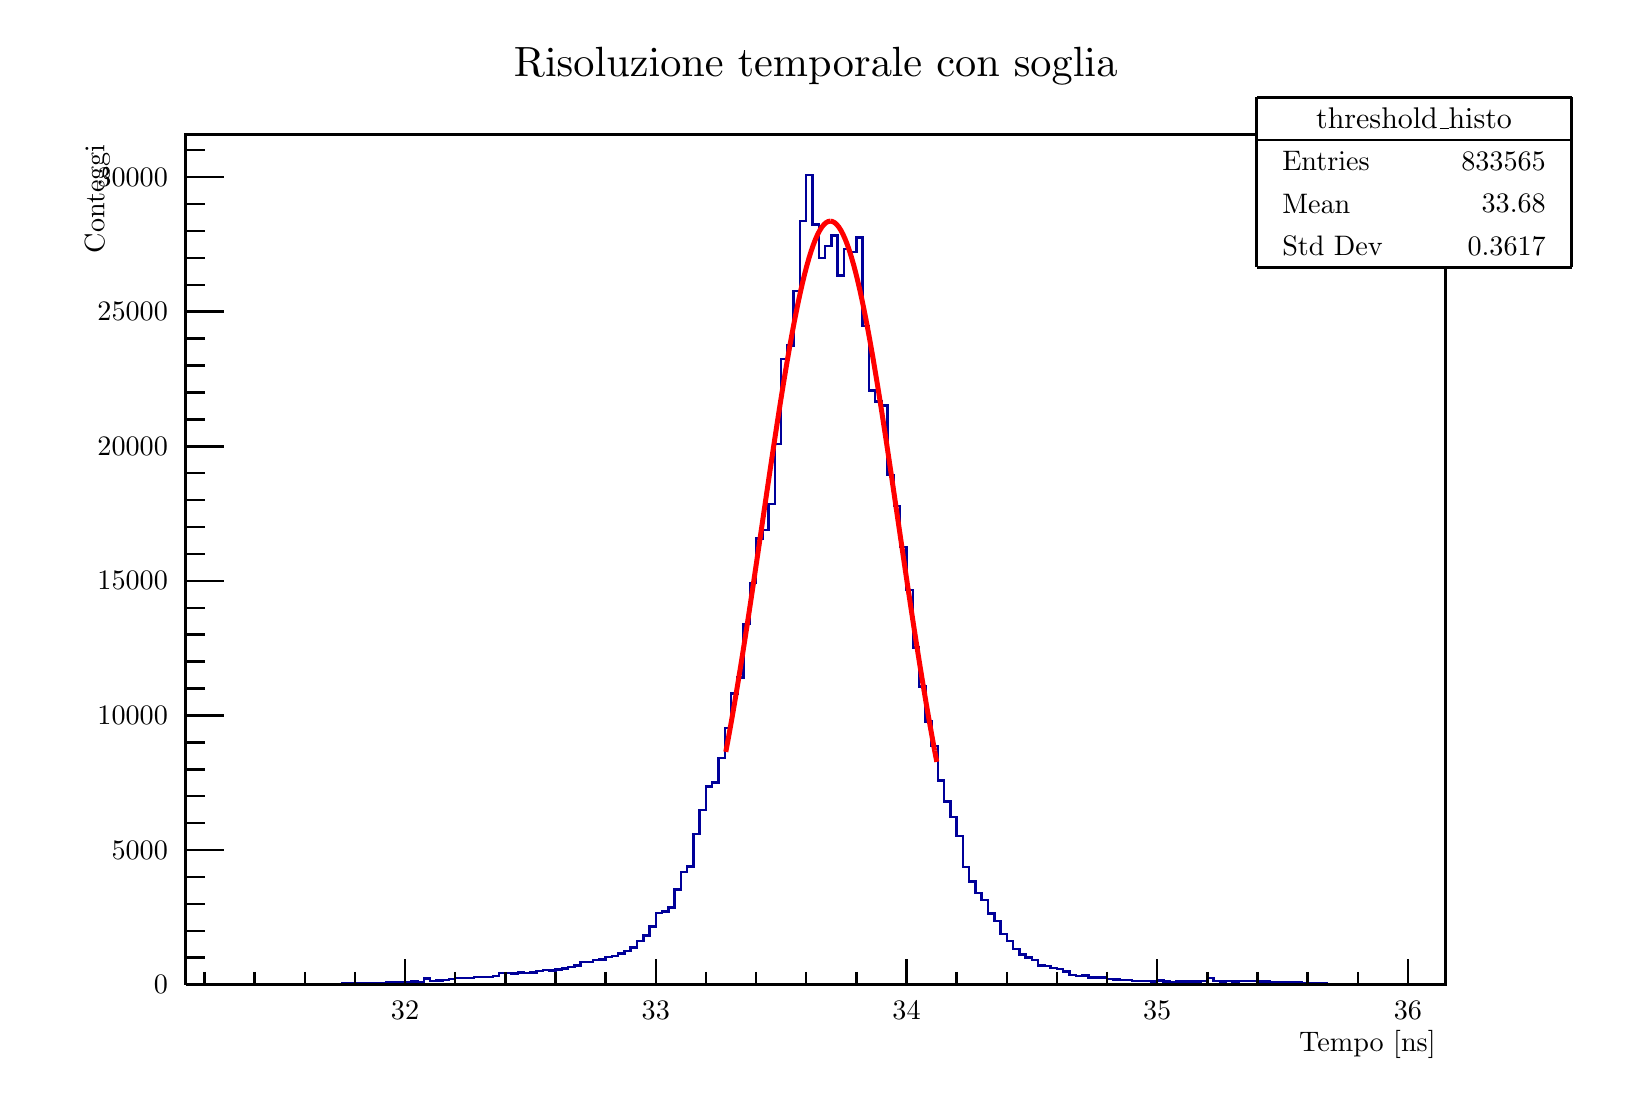
\begin{tikzpicture}
\pgfdeclareplotmark{cross} {
\pgfpathmoveto{\pgfpoint{-0.3\pgfplotmarksize}{\pgfplotmarksize}}
\pgfpathlineto{\pgfpoint{+0.3\pgfplotmarksize}{\pgfplotmarksize}}
\pgfpathlineto{\pgfpoint{+0.3\pgfplotmarksize}{0.3\pgfplotmarksize}}
\pgfpathlineto{\pgfpoint{+1\pgfplotmarksize}{0.3\pgfplotmarksize}}
\pgfpathlineto{\pgfpoint{+1\pgfplotmarksize}{-0.3\pgfplotmarksize}}
\pgfpathlineto{\pgfpoint{+0.3\pgfplotmarksize}{-0.3\pgfplotmarksize}}
\pgfpathlineto{\pgfpoint{+0.3\pgfplotmarksize}{-1.\pgfplotmarksize}}
\pgfpathlineto{\pgfpoint{-0.3\pgfplotmarksize}{-1.\pgfplotmarksize}}
\pgfpathlineto{\pgfpoint{-0.3\pgfplotmarksize}{-0.3\pgfplotmarksize}}
\pgfpathlineto{\pgfpoint{-1.\pgfplotmarksize}{-0.3\pgfplotmarksize}}
\pgfpathlineto{\pgfpoint{-1.\pgfplotmarksize}{0.3\pgfplotmarksize}}
\pgfpathlineto{\pgfpoint{-0.3\pgfplotmarksize}{0.3\pgfplotmarksize}}
\pgfpathclose
\pgfusepathqstroke
}
\pgfdeclareplotmark{cross*} {
\pgfpathmoveto{\pgfpoint{-0.3\pgfplotmarksize}{\pgfplotmarksize}}
\pgfpathlineto{\pgfpoint{+0.3\pgfplotmarksize}{\pgfplotmarksize}}
\pgfpathlineto{\pgfpoint{+0.3\pgfplotmarksize}{0.3\pgfplotmarksize}}
\pgfpathlineto{\pgfpoint{+1\pgfplotmarksize}{0.3\pgfplotmarksize}}
\pgfpathlineto{\pgfpoint{+1\pgfplotmarksize}{-0.3\pgfplotmarksize}}
\pgfpathlineto{\pgfpoint{+0.3\pgfplotmarksize}{-0.3\pgfplotmarksize}}
\pgfpathlineto{\pgfpoint{+0.3\pgfplotmarksize}{-1.\pgfplotmarksize}}
\pgfpathlineto{\pgfpoint{-0.3\pgfplotmarksize}{-1.\pgfplotmarksize}}
\pgfpathlineto{\pgfpoint{-0.3\pgfplotmarksize}{-0.3\pgfplotmarksize}}
\pgfpathlineto{\pgfpoint{-1.\pgfplotmarksize}{-0.3\pgfplotmarksize}}
\pgfpathlineto{\pgfpoint{-1.\pgfplotmarksize}{0.3\pgfplotmarksize}}
\pgfpathlineto{\pgfpoint{-0.3\pgfplotmarksize}{0.3\pgfplotmarksize}}
\pgfpathclose
\pgfusepathqfillstroke
}
\pgfdeclareplotmark{newstar} {
\pgfpathmoveto{\pgfqpoint{0pt}{\pgfplotmarksize}}
\pgfpathlineto{\pgfqpointpolar{44}{0.5\pgfplotmarksize}}
\pgfpathlineto{\pgfqpointpolar{18}{\pgfplotmarksize}}
\pgfpathlineto{\pgfqpointpolar{-20}{0.5\pgfplotmarksize}}
\pgfpathlineto{\pgfqpointpolar{-54}{\pgfplotmarksize}}
\pgfpathlineto{\pgfqpointpolar{-90}{0.5\pgfplotmarksize}}
\pgfpathlineto{\pgfqpointpolar{234}{\pgfplotmarksize}}
\pgfpathlineto{\pgfqpointpolar{198}{0.5\pgfplotmarksize}}
\pgfpathlineto{\pgfqpointpolar{162}{\pgfplotmarksize}}
\pgfpathlineto{\pgfqpointpolar{134}{0.5\pgfplotmarksize}}
\pgfpathclose
\pgfusepathqstroke
}
\pgfdeclareplotmark{newstar*} {
\pgfpathmoveto{\pgfqpoint{0pt}{\pgfplotmarksize}}
\pgfpathlineto{\pgfqpointpolar{44}{0.5\pgfplotmarksize}}
\pgfpathlineto{\pgfqpointpolar{18}{\pgfplotmarksize}}
\pgfpathlineto{\pgfqpointpolar{-20}{0.5\pgfplotmarksize}}
\pgfpathlineto{\pgfqpointpolar{-54}{\pgfplotmarksize}}
\pgfpathlineto{\pgfqpointpolar{-90}{0.5\pgfplotmarksize}}
\pgfpathlineto{\pgfqpointpolar{234}{\pgfplotmarksize}}
\pgfpathlineto{\pgfqpointpolar{198}{0.5\pgfplotmarksize}}
\pgfpathlineto{\pgfqpointpolar{162}{\pgfplotmarksize}}
\pgfpathlineto{\pgfqpointpolar{134}{0.5\pgfplotmarksize}}
\pgfpathclose
\pgfusepathqfillstroke
}
\definecolor{c}{rgb}{1,1,1};
\draw [color=c, fill=c] (0,0) rectangle (20,13.4957);
\draw [color=c, fill=c] (2,1.34957) rectangle (18,12.1461);
\definecolor{c}{rgb}{0,0,0};
\draw [c,line width=0.9] (2,1.34957) -- (2,12.1461) -- (18,12.1461) -- (18,1.34957) -- (2,1.34957);
\definecolor{c}{rgb}{1,1,1};
\draw [color=c, fill=c] (2,1.34957) rectangle (18,12.1461);
\definecolor{c}{rgb}{0,0,0};
\draw [c,line width=0.9] (2,1.34957) -- (2,12.1461) -- (18,12.1461) -- (18,1.34957) -- (2,1.34957);
\definecolor{c}{rgb}{0,0,0.6};
\draw [c,line width=0.9] (2,1.35846) -- (2.0796,1.35846) -- (2.0796,1.36051) -- (2.1592,1.36051) -- (2.1592,1.36017) -- (2.23881,1.36017) -- (2.23881,1.35675) -- (2.31841,1.35675) -- (2.31841,1.35948) -- (2.39801,1.35948) -- (2.39801,1.3588) --
 (2.47761,1.3588) -- (2.47761,1.35777) -- (2.55721,1.35777) -- (2.55721,1.35743) -- (2.63682,1.35743) -- (2.63682,1.35743) -- (2.71642,1.35743) -- (2.71642,1.3547) -- (2.79602,1.3547) -- (2.79602,1.35743) -- (2.87562,1.35743) -- (2.87562,1.35846) --
 (2.95522,1.35846) -- (2.95522,1.35504) -- (3.03483,1.35504) -- (3.03483,1.35948) -- (3.11443,1.35948) -- (3.11443,1.36017) -- (3.19403,1.36017) -- (3.19403,1.35572) -- (3.27363,1.35572) -- (3.27363,1.35504) -- (3.35323,1.35504) -- (3.35323,1.35777)
 -- (3.43284,1.35777) -- (3.43284,1.35607) -- (3.51244,1.35607) -- (3.51244,1.35846) -- (3.59204,1.35846) -- (3.59204,1.3588) -- (3.67164,1.3588) -- (3.67164,1.36051) -- (3.75124,1.36051) -- (3.75124,1.35812) -- (3.83085,1.35812) -- (3.83085,1.35983)
 -- (3.91045,1.35983) -- (3.91045,1.36051) -- (3.99005,1.36051) -- (3.99005,1.36153) -- (4.06965,1.36153) -- (4.06965,1.36393) -- (4.14925,1.36393) -- (4.14925,1.36427) -- (4.22886,1.36427) -- (4.22886,1.36974) -- (4.30846,1.36974) --
 (4.30846,1.36632) -- (4.38806,1.36632) -- (4.38806,1.37008) -- (4.46766,1.37008) -- (4.46766,1.37042) -- (4.54726,1.37042) -- (4.54726,1.38136) -- (4.62687,1.38136) -- (4.62687,1.3735) -- (4.70647,1.3735) -- (4.70647,1.38102) -- (4.78607,1.38102) --
 (4.78607,1.38546) -- (4.86567,1.38546) -- (4.86567,1.38922) -- (4.94527,1.38922) -- (4.94527,1.38581) -- (5.02488,1.38581) -- (5.02488,1.42956) -- (5.10448,1.42956) -- (5.10448,1.39435) -- (5.18408,1.39435) -- (5.18408,1.40153) -- (5.26368,1.40153)
 -- (5.26368,1.40734) -- (5.34328,1.40734) -- (5.34328,1.4217) -- (5.42289,1.4217) -- (5.42289,1.43059) -- (5.50249,1.43059) -- (5.50249,1.43469) -- (5.58209,1.43469) -- (5.58209,1.43161) -- (5.66169,1.43161) -- (5.66169,1.44768) -- (5.74129,1.44768)
 -- (5.74129,1.44939) -- (5.8209,1.44939) -- (5.8209,1.44836) -- (5.9005,1.44836) -- (5.9005,1.46033) -- (5.9801,1.46033) -- (5.9801,1.49554) -- (6.0597,1.49554) -- (6.0597,1.49554) -- (6.1393,1.49554) -- (6.1393,1.49007) -- (6.21891,1.49007) --
 (6.21891,1.50238) -- (6.29851,1.50238) -- (6.29851,1.49417) -- (6.37811,1.49417) -- (6.37811,1.50511) -- (6.45771,1.50511) -- (6.45771,1.52049) -- (6.53731,1.52049) -- (6.53731,1.53451) -- (6.61692,1.53451) -- (6.61692,1.53109) -- (6.69652,1.53109)
 -- (6.69652,1.54271) -- (6.77612,1.54271) -- (6.77612,1.55126) -- (6.85572,1.55126) -- (6.85572,1.57177) -- (6.93532,1.57177) -- (6.93532,1.59433) -- (7.01493,1.59433) -- (7.01493,1.63672) -- (7.09453,1.63672) -- (7.09453,1.63535) --
 (7.17413,1.63535) -- (7.17413,1.66441) -- (7.25373,1.66441) -- (7.25373,1.66954) -- (7.33333,1.66954) -- (7.33333,1.69928) -- (7.41294,1.69928) -- (7.41294,1.71193) -- (7.49254,1.71193) -- (7.49254,1.74338) -- (7.57214,1.74338) -- (7.57214,1.77449)
 -- (7.65174,1.77449) -- (7.65174,1.81961) -- (7.73134,1.81961) -- (7.73134,1.90268) -- (7.81095,1.90268) -- (7.81095,1.97276) -- (7.89055,1.97276) -- (7.89055,2.08933) -- (7.97015,2.08933) -- (7.97015,2.25752) -- (8.04975,2.25752) --
 (8.04975,2.27837) -- (8.12935,2.27837) -- (8.12935,2.33033) -- (8.20895,2.33033) -- (8.20895,2.55869) -- (8.28856,2.55869) -- (8.28856,2.78157) -- (8.36816,2.78157) -- (8.36816,2.84994) -- (8.44776,2.84994) -- (8.44776,3.26289) -- (8.52736,3.26289)
 -- (8.52736,3.5644) -- (8.60697,3.5644) -- (8.60697,3.86523) -- (8.68657,3.86523) -- (8.68657,3.91719) -- (8.76617,3.91719) -- (8.76617,4.23066) -- (8.84577,4.23066) -- (8.84577,4.61114) -- (8.92537,4.61114) -- (8.92537,5.04529) -- (9.00498,5.04529)
 -- (9.00498,5.24698) -- (9.08458,5.24698) -- (9.08458,5.92657) -- (9.16418,5.92657) -- (9.16418,6.44686) -- (9.24378,6.44686) -- (9.24378,7.01706) -- (9.32338,7.01706) -- (9.32338,7.1244) -- (9.40298,7.1244) -- (9.40298,7.45019) -- (9.48259,7.45019)
 -- (9.48259,8.21285) -- (9.56219,8.21285) -- (9.56219,9.29377) -- (9.64179,9.29377) -- (9.64179,9.46367) -- (9.72139,9.46367) -- (9.72139,10.1566) -- (9.80099,10.1566) -- (9.80099,11.0464) -- (9.8806,11.0464) -- (9.8806,11.632) -- (9.9602,11.632) --
 (9.9602,11.0037) -- (10.0398,11.0037) -- (10.0398,10.5774) -- (10.1194,10.5774) -- (10.1194,10.7319) -- (10.199,10.7319) -- (10.199,10.8615) -- (10.2786,10.8615) -- (10.2786,10.3555) -- (10.3582,10.3555) -- (10.3582,10.694) -- (10.4378,10.694) --
 (10.4378,10.6567) -- (10.5174,10.6567) -- (10.5174,10.8352) -- (10.597,10.8352) -- (10.597,9.71493) -- (10.6766,9.71493) -- (10.6766,8.89278) -- (10.7562,8.89278) -- (10.7562,8.75604) -- (10.8358,8.75604) -- (10.8358,8.70579) -- (10.9154,8.70579) --
 (10.9154,7.81938) -- (10.995,7.81938) -- (10.995,7.42831) -- (11.0746,7.42831) -- (11.0746,6.90425) -- (11.1542,6.90425) -- (11.1542,6.35935) -- (11.2338,6.35935) -- (11.2338,5.63361) -- (11.3134,5.63361) -- (11.3134,5.1369) -- (11.393,5.1369) --
 (11.393,4.68942) -- (11.4726,4.68942) -- (11.4726,4.378) -- (11.5522,4.378) -- (11.5522,3.94078) -- (11.6318,3.94078) -- (11.6318,3.67277) -- (11.7114,3.67277) -- (11.7114,3.47894) -- (11.791,3.47894) -- (11.791,3.23965) -- (11.8706,3.23965) --
 (11.8706,2.84618) -- (11.9502,2.84618) -- (11.9502,2.66021) -- (12.0299,2.66021) -- (12.0299,2.51219) -- (12.1095,2.51219) -- (12.1095,2.42673) -- (12.1891,2.42673) -- (12.1891,2.25547) -- (12.2687,2.25547) -- (12.2687,2.15462) -- (12.3483,2.15462)
 -- (12.3483,1.99019) -- (12.4279,1.99019) -- (12.4279,1.90097) -- (12.5075,1.90097) -- (12.5075,1.80252) -- (12.5871,1.80252) -- (12.5871,1.73347) -- (12.6667,1.73347) -- (12.6667,1.69484) -- (12.7463,1.69484) -- (12.7463,1.65894) --
 (12.8259,1.65894) -- (12.8259,1.59399) -- (12.9055,1.59399) -- (12.9055,1.58784) -- (12.9851,1.58784) -- (12.9851,1.55878) -- (13.0647,1.55878) -- (13.0647,1.54784) -- (13.1443,1.54784) -- (13.1443,1.51913) -- (13.2239,1.51913) -- (13.2239,1.46956)
 -- (13.3035,1.46956) -- (13.3035,1.45759) -- (13.3831,1.45759) -- (13.3831,1.46511) -- (13.4627,1.46511) -- (13.4627,1.43845) -- (13.5423,1.43845) -- (13.5423,1.43913) -- (13.6219,1.43913) -- (13.6219,1.43811) -- (13.7015,1.43811) --
 (13.7015,1.42204) -- (13.7811,1.42204) -- (13.7811,1.41179) -- (13.8607,1.41179) -- (13.8607,1.40871) -- (13.9403,1.40871) -- (13.9403,1.40734) -- (14.0199,1.40734) -- (14.0199,1.39811) -- (14.0995,1.39811) -- (14.0995,1.39367) -- (14.1791,1.39367)
 -- (14.1791,1.39743) -- (14.2587,1.39743) -- (14.2587,1.39162) -- (14.3383,1.39162) -- (14.3383,1.39982) -- (14.4179,1.39982) -- (14.4179,1.39196) -- (14.4975,1.39196) -- (14.4975,1.38581) -- (14.5771,1.38581) -- (14.5771,1.38991) --
 (14.6567,1.38991) -- (14.6567,1.3882) -- (14.7363,1.3882) -- (14.7363,1.38888) -- (14.8159,1.38888) -- (14.8159,1.39128) -- (14.8955,1.39128) -- (14.8955,1.39469) -- (14.9751,1.39469) -- (14.9751,1.4364) -- (15.0547,1.4364) -- (15.0547,1.39333) --
 (15.1343,1.39333) -- (15.1343,1.38854) -- (15.2139,1.38854) -- (15.2139,1.3923) -- (15.2935,1.3923) -- (15.2935,1.38854) -- (15.3731,1.38854) -- (15.3731,1.39401) -- (15.4527,1.39401) -- (15.4527,1.39675) -- (15.5323,1.39675) -- (15.5323,1.39504) --
 (15.6119,1.39504) -- (15.6119,1.38683) -- (15.6915,1.38683) -- (15.6915,1.39059) -- (15.7711,1.39059) -- (15.7711,1.38205) -- (15.8507,1.38205) -- (15.8507,1.38239) -- (15.9303,1.38239) -- (15.9303,1.37623) -- (16.01,1.37623) -- (16.01,1.37897) --
 (16.0896,1.37897) -- (16.0896,1.38136) -- (16.1692,1.38136) -- (16.1692,1.36906) -- (16.2488,1.36906) -- (16.2488,1.37316) -- (16.3284,1.37316) -- (16.3284,1.36666) -- (16.408,1.36666) -- (16.408,1.36256) -- (16.4876,1.36256) -- (16.4876,1.35948) --
 (16.5672,1.35948) -- (16.5672,1.36051) -- (16.6468,1.36051) -- (16.6468,1.35743) -- (16.7264,1.35743) -- (16.7264,1.35743) -- (16.806,1.35743) -- (16.806,1.35401) -- (16.8856,1.35401) -- (16.8856,1.35504) -- (16.9652,1.35504) -- (16.9652,1.35436) --
 (17.0448,1.35436) -- (17.0448,1.35333) -- (17.1244,1.35333) -- (17.1244,1.35231) -- (17.204,1.35231) -- (17.204,1.35128) -- (17.2836,1.35128) -- (17.2836,1.35436) -- (17.3632,1.35436) -- (17.3632,1.35162) -- (17.4428,1.35162) -- (17.4428,1.35128) --
 (17.5224,1.35128) -- (17.5224,1.35094) -- (17.602,1.35094) -- (17.602,1.35025) -- (17.6816,1.35025) -- (17.6816,1.35025) -- (17.7612,1.35025) -- (17.7612,1.35196) -- (17.8408,1.35196) -- (17.8408,1.35025) -- (17.9204,1.35025) -- (17.9204,1.35231) --
 (18,1.35231);
\definecolor{c}{rgb}{1,1,1};
\draw [color=c, fill=c] (15.6,10.4592) rectangle (19.6,12.6185);
\definecolor{c}{rgb}{0,0,0};
\draw [c,line width=0.9] (15.6,10.4592) -- (19.6,10.4592);
\draw [c,line width=0.9] (19.6,10.4592) -- (19.6,12.6185);
\draw [c,line width=0.9] (19.6,12.6185) -- (15.6,12.6185);
\draw [c,line width=0.9] (15.6,12.6185) -- (15.6,10.4592);
\draw (17.6,12.3486) node[scale=1.08185, color=c, rotate=0]{threshold\_histo};
\draw [c,line width=0.9] (15.6,12.0787) -- (19.6,12.0787);
\draw [anchor= west] (15.8,11.8087) node[scale=1.01821, color=c, rotate=0]{Entries };
\draw [anchor= east] (19.4,11.8087) node[scale=1.01821, color=c, rotate=0]{ 833565};
\draw [anchor= west] (15.8,11.2689) node[scale=1.01821, color=c, rotate=0]{Mean  };
\draw [anchor= east] (19.4,11.2689) node[scale=1.01821, color=c, rotate=0]{  33.68};
\draw [anchor= west] (15.8,10.7291) node[scale=1.01821, color=c, rotate=0]{Std Dev   };
\draw [anchor= east] (19.4,10.7291) node[scale=1.01821, color=c, rotate=0]{ 0.3617};
\definecolor{c}{rgb}{1,0,0};
\draw [c,line width=1.8] (8.8593,4.30538) -- (8.88637,4.45054) -- (8.91343,4.59962) -- (8.9405,4.75251) -- (8.96756,4.90907) -- (8.99463,5.06916) -- (9.02169,5.23261) -- (9.04876,5.39925) -- (9.07582,5.56886) -- (9.10289,5.74125) -- (9.12995,5.91616)
 -- (9.15701,6.09335) -- (9.18408,6.27256) -- (9.21114,6.45349) -- (9.23821,6.63586) -- (9.26527,6.81933) -- (9.29234,7.00358) -- (9.3194,7.18828) -- (9.34647,7.37305) -- (9.37353,7.55754) -- (9.4006,7.74136) -- (9.42766,7.92414) -- (9.45473,8.10546)
 -- (9.48179,8.28494) -- (9.50886,8.46215) -- (9.53592,8.63669) -- (9.56299,8.80815) -- (9.59005,8.97611) -- (9.61711,9.14015) -- (9.64418,9.29987) -- (9.67124,9.45485) -- (9.69831,9.6047) -- (9.72537,9.74902) -- (9.75244,9.88743) -- (9.7795,10.0196)
 -- (9.80657,10.145) -- (9.83363,10.2635) -- (9.8607,10.3747) -- (9.88776,10.4782) -- (9.91483,10.5738) -- (9.94189,10.6613) -- (9.96896,10.7402) -- (9.99602,10.8105) -- (10.0231,10.8719) -- (10.0501,10.9243) -- (10.0772,10.9674) -- (10.1043,11.0012)
 -- (10.1313,11.0255) -- (10.1584,11.0404) -- (10.1855,11.0456);
\draw [c,line width=1.8] (10.1855,11.0456) -- (10.2125,11.0413) -- (10.2396,11.0275) -- (10.2667,11.0041) -- (10.2937,10.9713) -- (10.3208,10.9291) -- (10.3479,10.8777) -- (10.3749,10.8172) -- (10.402,10.7479) -- (10.4291,10.6698) --
 (10.4561,10.5832) -- (10.4832,10.4884) -- (10.5102,10.3857) -- (10.5373,10.2753) -- (10.5644,10.1576) -- (10.5914,10.0328) -- (10.6185,9.90132) -- (10.6456,9.76354) -- (10.6726,9.61981) -- (10.6997,9.47052) -- (10.7268,9.31604) -- (10.7538,9.15679)
 -- (10.7809,8.99318) -- (10.808,8.8256) -- (10.835,8.65448) -- (10.8621,8.48024) -- (10.8892,8.30328) -- (10.9162,8.12402) -- (10.9433,7.94287) -- (10.9703,7.76022) -- (10.9974,7.57649) -- (11.0245,7.39205) -- (11.0515,7.20729) -- (11.0786,7.02257)
 -- (11.1057,6.83825) -- (11.1327,6.65469) -- (11.1598,6.4722) -- (11.1869,6.2911) -- (11.2139,6.1117) -- (11.241,5.93429) -- (11.2681,5.75913) -- (11.2951,5.58647) -- (11.3222,5.41656) -- (11.3493,5.24961) -- (11.3763,5.08582) -- (11.4034,4.92538)
 -- (11.4304,4.76845) -- (11.4575,4.61518) -- (11.4846,4.4657) -- (11.5116,4.32013);
\draw [c,line width=1.8] (11.5116,4.32013) -- (11.5387,4.17856);
\definecolor{c}{rgb}{0,0,0};
\draw [c,line width=0.9] (2,1.34957) -- (18,1.34957);
\draw [anchor= east] (18,0.593811) node[scale=1.01821, color=c, rotate=0]{Tempo [ns]};
\draw [c,line width=0.9] (4.78607,1.67347) -- (4.78607,1.34957);
\draw [c,line width=0.9] (5.42289,1.51152) -- (5.42289,1.34957);
\draw [c,line width=0.9] (6.0597,1.51152) -- (6.0597,1.34957);
\draw [c,line width=0.9] (6.69652,1.51152) -- (6.69652,1.34957);
\draw [c,line width=0.9] (7.33333,1.51152) -- (7.33333,1.34957);
\draw [c,line width=0.9] (7.97015,1.67347) -- (7.97015,1.34957);
\draw [c,line width=0.9] (8.60697,1.51152) -- (8.60697,1.34957);
\draw [c,line width=0.9] (9.24378,1.51152) -- (9.24378,1.34957);
\draw [c,line width=0.9] (9.8806,1.51152) -- (9.8806,1.34957);
\draw [c,line width=0.9] (10.5174,1.51152) -- (10.5174,1.34957);
\draw [c,line width=0.9] (11.1542,1.67347) -- (11.1542,1.34957);
\draw [c,line width=0.9] (11.791,1.51152) -- (11.791,1.34957);
\draw [c,line width=0.9] (12.4279,1.51152) -- (12.4279,1.34957);
\draw [c,line width=0.9] (13.0647,1.51152) -- (13.0647,1.34957);
\draw [c,line width=0.9] (13.7015,1.51152) -- (13.7015,1.34957);
\draw [c,line width=0.9] (14.3383,1.67347) -- (14.3383,1.34957);
\draw [c,line width=0.9] (14.9751,1.51152) -- (14.9751,1.34957);
\draw [c,line width=0.9] (15.6119,1.51152) -- (15.6119,1.34957);
\draw [c,line width=0.9] (16.2488,1.51152) -- (16.2488,1.34957);
\draw [c,line width=0.9] (16.8856,1.51152) -- (16.8856,1.34957);
\draw [c,line width=0.9] (17.5224,1.67347) -- (17.5224,1.34957);
\draw [c,line width=0.9] (4.78607,1.67347) -- (4.78607,1.34957);
\draw [c,line width=0.9] (4.14925,1.51152) -- (4.14925,1.34957);
\draw [c,line width=0.9] (3.51244,1.51152) -- (3.51244,1.34957);
\draw [c,line width=0.9] (2.87562,1.51152) -- (2.87562,1.34957);
\draw [c,line width=0.9] (2.23881,1.51152) -- (2.23881,1.34957);
\draw [c,line width=0.9] (17.5224,1.67347) -- (17.5224,1.34957);
\draw [anchor=base] (4.78607,0.904212) node[scale=1.01821, color=c, rotate=0]{32};
\draw [anchor=base] (7.97015,0.904212) node[scale=1.01821, color=c, rotate=0]{33};
\draw [anchor=base] (11.1542,0.904212) node[scale=1.01821, color=c, rotate=0]{34};
\draw [anchor=base] (14.3383,0.904212) node[scale=1.01821, color=c, rotate=0]{35};
\draw [anchor=base] (17.5224,0.904212) node[scale=1.01821, color=c, rotate=0]{36};
\draw [c,line width=0.9] (2,1.34957) -- (2,12.1461);
\draw [anchor= east] (0.88,12.1461) node[scale=1.01821, color=c, rotate=90]{Conteggi};
\draw [c,line width=0.9] (2.48,1.34957) -- (2,1.34957);
\draw [c,line width=0.9] (2.24,1.69142) -- (2,1.69142);
\draw [c,line width=0.9] (2.24,2.03327) -- (2,2.03327);
\draw [c,line width=0.9] (2.24,2.37511) -- (2,2.37511);
\draw [c,line width=0.9] (2.24,2.71696) -- (2,2.71696);
\draw [c,line width=0.9] (2.48,3.05881) -- (2,3.05881);
\draw [c,line width=0.9] (2.24,3.40066) -- (2,3.40066);
\draw [c,line width=0.9] (2.24,3.7425) -- (2,3.7425);
\draw [c,line width=0.9] (2.24,4.08435) -- (2,4.08435);
\draw [c,line width=0.9] (2.24,4.4262) -- (2,4.4262);
\draw [c,line width=0.9] (2.48,4.76805) -- (2,4.76805);
\draw [c,line width=0.9] (2.24,5.1099) -- (2,5.1099);
\draw [c,line width=0.9] (2.24,5.45174) -- (2,5.45174);
\draw [c,line width=0.9] (2.24,5.79359) -- (2,5.79359);
\draw [c,line width=0.9] (2.24,6.13544) -- (2,6.13544);
\draw [c,line width=0.9] (2.48,6.47729) -- (2,6.47729);
\draw [c,line width=0.9] (2.24,6.81913) -- (2,6.81913);
\draw [c,line width=0.9] (2.24,7.16098) -- (2,7.16098);
\draw [c,line width=0.9] (2.24,7.50283) -- (2,7.50283);
\draw [c,line width=0.9] (2.24,7.84468) -- (2,7.84468);
\draw [c,line width=0.9] (2.48,8.18653) -- (2,8.18653);
\draw [c,line width=0.9] (2.24,8.52837) -- (2,8.52837);
\draw [c,line width=0.9] (2.24,8.87022) -- (2,8.87022);
\draw [c,line width=0.9] (2.24,9.21207) -- (2,9.21207);
\draw [c,line width=0.9] (2.24,9.55392) -- (2,9.55392);
\draw [c,line width=0.9] (2.48,9.89576) -- (2,9.89576);
\draw [c,line width=0.9] (2.24,10.2376) -- (2,10.2376);
\draw [c,line width=0.9] (2.24,10.5795) -- (2,10.5795);
\draw [c,line width=0.9] (2.24,10.9213) -- (2,10.9213);
\draw [c,line width=0.9] (2.24,11.2632) -- (2,11.2632);
\draw [c,line width=0.9] (2.48,11.605) -- (2,11.605);
\draw [c,line width=0.9] (2.48,11.605) -- (2,11.605);
\draw [c,line width=0.9] (2.24,11.9469) -- (2,11.9469);
\draw [anchor= east] (1.9,1.34957) node[scale=1.01821, color=c, rotate=0]{0};
\draw [anchor= east] (1.9,3.05881) node[scale=1.01821, color=c, rotate=0]{5000};
\draw [anchor= east] (1.9,4.76805) node[scale=1.01821, color=c, rotate=0]{10000};
\draw [anchor= east] (1.9,6.47729) node[scale=1.01821, color=c, rotate=0]{15000};
\draw [anchor= east] (1.9,8.18653) node[scale=1.01821, color=c, rotate=0]{20000};
\draw [anchor= east] (1.9,9.89576) node[scale=1.01821, color=c, rotate=0]{25000};
\draw [anchor= east] (1.9,11.605) node[scale=1.01821, color=c, rotate=0]{30000};
\definecolor{c}{rgb}{1,1,1};
\draw [color=c, fill=c] (15.6,10.4592) rectangle (19.6,12.6185);
\definecolor{c}{rgb}{0,0,0};
\draw [c,line width=0.9] (15.6,10.4592) -- (19.6,10.4592);
\draw [c,line width=0.9] (19.6,10.4592) -- (19.6,12.6185);
\draw [c,line width=0.9] (19.6,12.6185) -- (15.6,12.6185);
\draw [c,line width=0.9] (15.6,12.6185) -- (15.6,10.4592);
\draw (17.6,12.3486) node[scale=1.08185, color=c, rotate=0]{threshold\_histo};
\draw [c,line width=0.9] (15.6,12.0787) -- (19.6,12.0787);
\draw [anchor= west] (15.8,11.8087) node[scale=1.01821, color=c, rotate=0]{Entries };
\draw [anchor= east] (19.4,11.8087) node[scale=1.01821, color=c, rotate=0]{ 833565};
\draw [anchor= west] (15.8,11.2689) node[scale=1.01821, color=c, rotate=0]{Mean  };
\draw [anchor= east] (19.4,11.2689) node[scale=1.01821, color=c, rotate=0]{  33.68};
\draw [anchor= west] (15.8,10.7291) node[scale=1.01821, color=c, rotate=0]{Std Dev   };
\draw [anchor= east] (19.4,10.7291) node[scale=1.01821, color=c, rotate=0]{ 0.3617};
\draw (10,13.0156) node[scale=1.52731, color=c, rotate=0]{Risoluzione temporale con soglia};
\end{tikzpicture}

%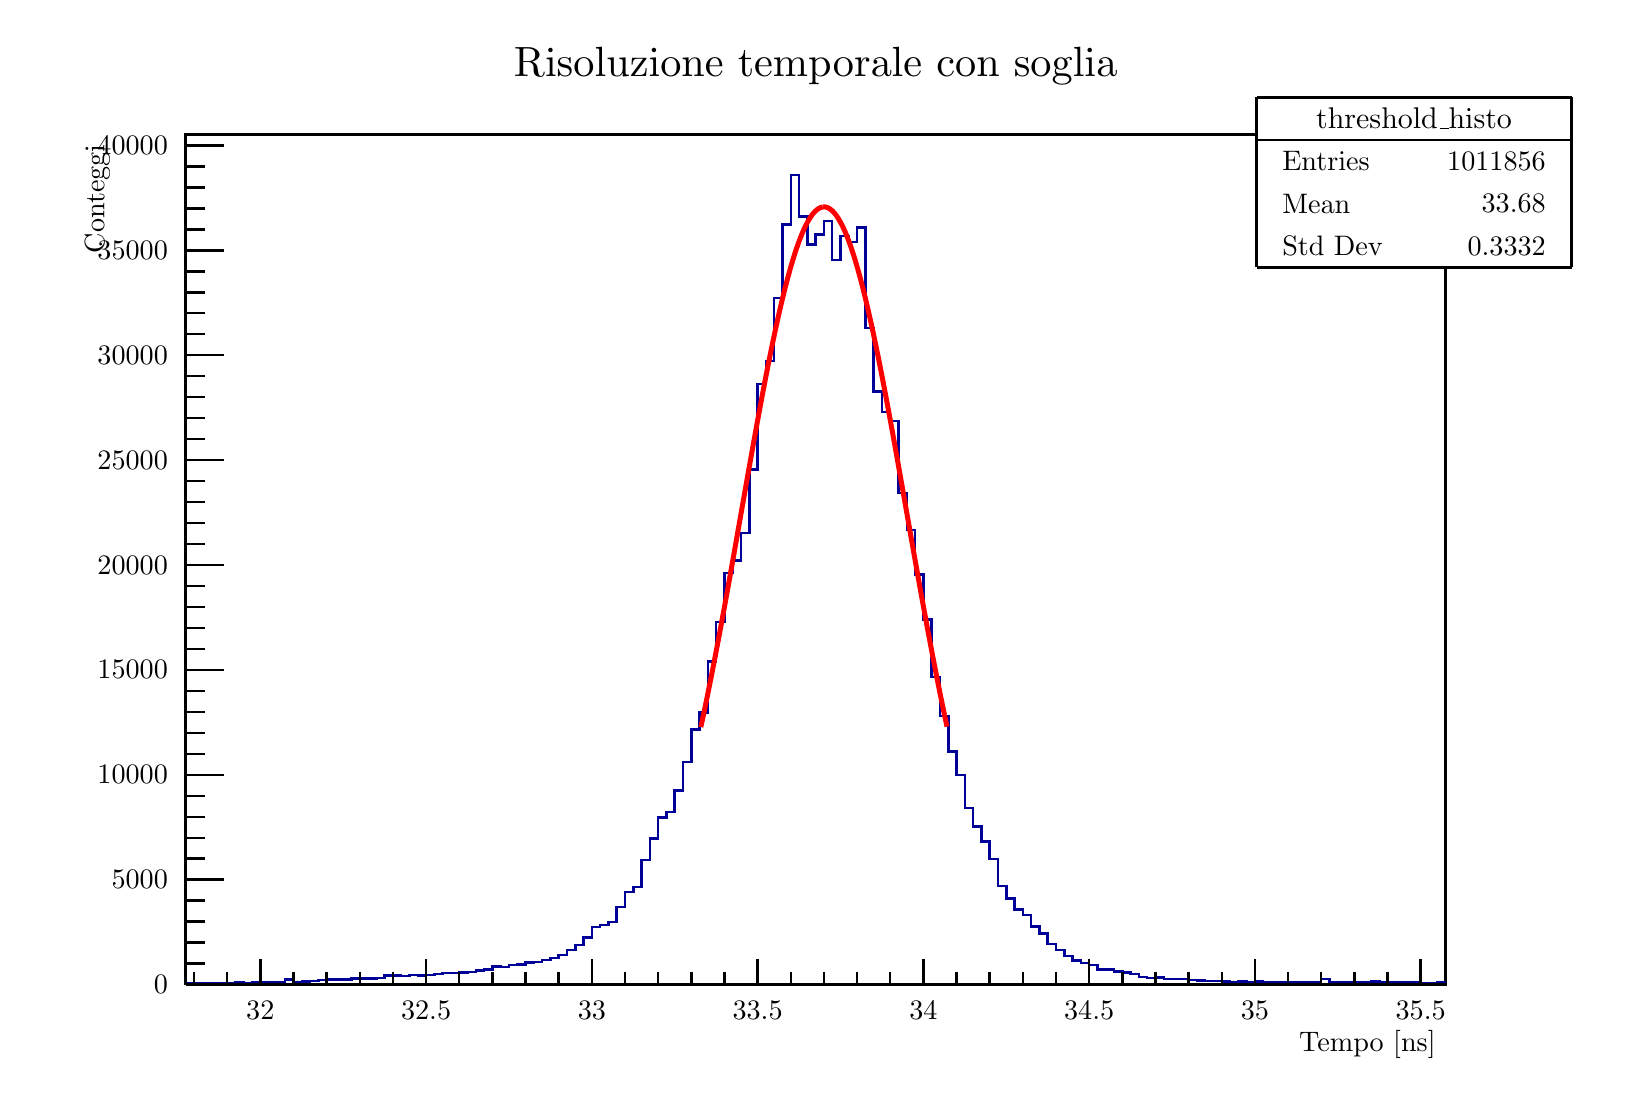
\begin{tikzpicture}
\pgfdeclareplotmark{cross} {
\pgfpathmoveto{\pgfpoint{-0.3\pgfplotmarksize}{\pgfplotmarksize}}
\pgfpathlineto{\pgfpoint{+0.3\pgfplotmarksize}{\pgfplotmarksize}}
\pgfpathlineto{\pgfpoint{+0.3\pgfplotmarksize}{0.3\pgfplotmarksize}}
\pgfpathlineto{\pgfpoint{+1\pgfplotmarksize}{0.3\pgfplotmarksize}}
\pgfpathlineto{\pgfpoint{+1\pgfplotmarksize}{-0.3\pgfplotmarksize}}
\pgfpathlineto{\pgfpoint{+0.3\pgfplotmarksize}{-0.3\pgfplotmarksize}}
\pgfpathlineto{\pgfpoint{+0.3\pgfplotmarksize}{-1.\pgfplotmarksize}}
\pgfpathlineto{\pgfpoint{-0.3\pgfplotmarksize}{-1.\pgfplotmarksize}}
\pgfpathlineto{\pgfpoint{-0.3\pgfplotmarksize}{-0.3\pgfplotmarksize}}
\pgfpathlineto{\pgfpoint{-1.\pgfplotmarksize}{-0.3\pgfplotmarksize}}
\pgfpathlineto{\pgfpoint{-1.\pgfplotmarksize}{0.3\pgfplotmarksize}}
\pgfpathlineto{\pgfpoint{-0.3\pgfplotmarksize}{0.3\pgfplotmarksize}}
\pgfpathclose
\pgfusepathqstroke
}
\pgfdeclareplotmark{cross*} {
\pgfpathmoveto{\pgfpoint{-0.3\pgfplotmarksize}{\pgfplotmarksize}}
\pgfpathlineto{\pgfpoint{+0.3\pgfplotmarksize}{\pgfplotmarksize}}
\pgfpathlineto{\pgfpoint{+0.3\pgfplotmarksize}{0.3\pgfplotmarksize}}
\pgfpathlineto{\pgfpoint{+1\pgfplotmarksize}{0.3\pgfplotmarksize}}
\pgfpathlineto{\pgfpoint{+1\pgfplotmarksize}{-0.3\pgfplotmarksize}}
\pgfpathlineto{\pgfpoint{+0.3\pgfplotmarksize}{-0.3\pgfplotmarksize}}
\pgfpathlineto{\pgfpoint{+0.3\pgfplotmarksize}{-1.\pgfplotmarksize}}
\pgfpathlineto{\pgfpoint{-0.3\pgfplotmarksize}{-1.\pgfplotmarksize}}
\pgfpathlineto{\pgfpoint{-0.3\pgfplotmarksize}{-0.3\pgfplotmarksize}}
\pgfpathlineto{\pgfpoint{-1.\pgfplotmarksize}{-0.3\pgfplotmarksize}}
\pgfpathlineto{\pgfpoint{-1.\pgfplotmarksize}{0.3\pgfplotmarksize}}
\pgfpathlineto{\pgfpoint{-0.3\pgfplotmarksize}{0.3\pgfplotmarksize}}
\pgfpathclose
\pgfusepathqfillstroke
}
\pgfdeclareplotmark{newstar} {
\pgfpathmoveto{\pgfqpoint{0pt}{\pgfplotmarksize}}
\pgfpathlineto{\pgfqpointpolar{44}{0.5\pgfplotmarksize}}
\pgfpathlineto{\pgfqpointpolar{18}{\pgfplotmarksize}}
\pgfpathlineto{\pgfqpointpolar{-20}{0.5\pgfplotmarksize}}
\pgfpathlineto{\pgfqpointpolar{-54}{\pgfplotmarksize}}
\pgfpathlineto{\pgfqpointpolar{-90}{0.5\pgfplotmarksize}}
\pgfpathlineto{\pgfqpointpolar{234}{\pgfplotmarksize}}
\pgfpathlineto{\pgfqpointpolar{198}{0.5\pgfplotmarksize}}
\pgfpathlineto{\pgfqpointpolar{162}{\pgfplotmarksize}}
\pgfpathlineto{\pgfqpointpolar{134}{0.5\pgfplotmarksize}}
\pgfpathclose
\pgfusepathqstroke
}
\pgfdeclareplotmark{newstar*} {
\pgfpathmoveto{\pgfqpoint{0pt}{\pgfplotmarksize}}
\pgfpathlineto{\pgfqpointpolar{44}{0.5\pgfplotmarksize}}
\pgfpathlineto{\pgfqpointpolar{18}{\pgfplotmarksize}}
\pgfpathlineto{\pgfqpointpolar{-20}{0.5\pgfplotmarksize}}
\pgfpathlineto{\pgfqpointpolar{-54}{\pgfplotmarksize}}
\pgfpathlineto{\pgfqpointpolar{-90}{0.5\pgfplotmarksize}}
\pgfpathlineto{\pgfqpointpolar{234}{\pgfplotmarksize}}
\pgfpathlineto{\pgfqpointpolar{198}{0.5\pgfplotmarksize}}
\pgfpathlineto{\pgfqpointpolar{162}{\pgfplotmarksize}}
\pgfpathlineto{\pgfqpointpolar{134}{0.5\pgfplotmarksize}}
\pgfpathclose
\pgfusepathqfillstroke
}
\definecolor{c}{rgb}{1,1,1};
\draw [color=c, fill=c] (0,0) rectangle (20,13.4957);
\draw [color=c, fill=c] (2,1.34957) rectangle (18,12.1461);
\definecolor{c}{rgb}{0,0,0};
\draw [c,line width=0.9] (2,1.34957) -- (2,12.1461) -- (18,12.1461) -- (18,1.34957) -- (2,1.34957);
\definecolor{c}{rgb}{1,1,1};
\draw [color=c, fill=c] (2,1.34957) rectangle (18,12.1461);
\definecolor{c}{rgb}{0,0,0};
\draw [c,line width=0.9] (2,1.34957) -- (2,12.1461) -- (18,12.1461) -- (18,1.34957) -- (2,1.34957);
\definecolor{c}{rgb}{0,0,0.6};
\draw [c,line width=0.9] (2,1.36103) -- (2.10526,1.36103) -- (2.10526,1.36183) -- (2.21053,1.36183) -- (2.21053,1.36529) -- (2.31579,1.36529) -- (2.31579,1.36263) -- (2.42105,1.36263) -- (2.42105,1.36556) -- (2.52632,1.36556) -- (2.52632,1.36609) --
 (2.63158,1.36609) -- (2.63158,1.37462) -- (2.73684,1.37462) -- (2.73684,1.36849) -- (2.84211,1.36849) -- (2.84211,1.37408) -- (2.94737,1.37408) -- (2.94737,1.37755) -- (3.05263,1.37755) -- (3.05263,1.38048) -- (3.15789,1.38048) -- (3.15789,1.37808)
 -- (3.26316,1.37808) -- (3.26316,1.41192) -- (3.36842,1.41192) -- (3.36842,1.38474) -- (3.47368,1.38474) -- (3.47368,1.39034) -- (3.57895,1.39034) -- (3.57895,1.3954) -- (3.68421,1.3954) -- (3.68421,1.40606) -- (3.78947,1.40606) -- (3.78947,1.41352)
 -- (3.89474,1.41352) -- (3.89474,1.41618) -- (4,1.41618) -- (4,1.41405) -- (4.10526,1.41405) -- (4.10526,1.42764) -- (4.21053,1.42764) -- (4.21053,1.42844) -- (4.31579,1.42844) -- (4.31579,1.42737) -- (4.42105,1.42737) -- (4.42105,1.4367) --
 (4.52632,1.4367) -- (4.52632,1.46521) -- (4.63158,1.46521) -- (4.63158,1.46468) -- (4.73684,1.46468) -- (4.73684,1.46094) -- (4.84211,1.46094) -- (4.84211,1.46974) -- (4.94737,1.46974) -- (4.94737,1.46441) -- (5.05263,1.46441) -- (5.05263,1.47187)
 -- (5.15789,1.47187) -- (5.15789,1.48519) -- (5.26316,1.48519) -- (5.26316,1.49532) -- (5.36842,1.49532) -- (5.36842,1.49398) -- (5.47368,1.49398) -- (5.47368,1.50304) -- (5.57895,1.50304) -- (5.57895,1.5097) -- (5.68421,1.5097) -- (5.68421,1.52596)
 -- (5.78947,1.52596) -- (5.78947,1.54328) -- (5.89474,1.54328) -- (5.89474,1.57685) -- (6,1.57685) -- (6,1.57418) -- (6.10526,1.57418) -- (6.10526,1.6003) -- (6.21053,1.6003) -- (6.21053,1.60403) -- (6.31579,1.60403) -- (6.31579,1.62747) --
 (6.42105,1.62747) -- (6.42105,1.63787) -- (6.52632,1.63787) -- (6.52632,1.66531) -- (6.63158,1.66531) -- (6.63158,1.68796) -- (6.73684,1.68796) -- (6.73684,1.72633) -- (6.84211,1.72633) -- (6.84211,1.79187) -- (6.94737,1.79187) -- (6.94737,1.85235)
 -- (7.05263,1.85235) -- (7.05263,1.94721) -- (7.15789,1.94721) -- (7.15789,2.0831) -- (7.26316,2.0831) -- (7.26316,2.10974) -- (7.36842,2.10974) -- (7.36842,2.14625) -- (7.47368,2.14625) -- (7.47368,2.33809) -- (7.57895,2.33809) -- (7.57895,2.52433)
 -- (7.68421,2.52433) -- (7.68421,2.58695) -- (7.78947,2.58695) -- (7.78947,2.93173) -- (7.89474,2.93173) -- (7.89474,3.2059) -- (8,3.2059) -- (8,3.47208) -- (8.10526,3.47208) -- (8.10526,3.54243) -- (8.21053,3.54243) -- (8.21053,3.81207) --
 (8.31579,3.81207) -- (8.31579,4.1747) -- (8.42105,4.1747) -- (8.42105,4.58876) -- (8.52632,4.58876) -- (8.52632,4.80458) -- (8.63158,4.80458) -- (8.63158,5.45445) -- (8.73684,5.45445) -- (8.73684,5.95616) -- (8.8421,5.95616) -- (8.8421,6.57592) --
 (8.94737,6.57592) -- (8.94737,6.73579) -- (9.05263,6.73579) -- (9.05263,7.0867) -- (9.1579,7.0867) -- (9.1579,7.89083) -- (9.26316,7.89083) -- (9.26316,8.97634) -- (9.36842,8.97634) -- (9.36842,9.26916) -- (9.47368,9.26916) -- (9.47368,10.0698) --
 (9.57895,10.0698) -- (9.57895,11.0024) -- (9.68421,11.0024) -- (9.68421,11.632) -- (9.78947,11.632) -- (9.78947,11.1044) -- (9.89474,11.1044) -- (9.89474,10.7463) -- (10,10.7463) -- (10,10.8756) -- (10.1053,10.8756) -- (10.1053,11.048) --
 (10.2105,11.048) -- (10.2105,10.5508) -- (10.3158,10.5508) -- (10.3158,10.8574) -- (10.4211,10.8574) -- (10.4211,10.7788) -- (10.5263,10.7788) -- (10.5263,10.9619) -- (10.6316,10.9619) -- (10.6316,9.68935) -- (10.7368,9.68935) -- (10.7368,8.88175)
 -- (10.8421,8.88175) -- (10.8421,8.62303) -- (10.9474,8.62303) -- (10.9474,8.50499) -- (11.0526,8.50499) -- (11.0526,7.59241) -- (11.1579,7.59241) -- (11.1579,7.12587) -- (11.2632,7.12587) -- (11.2632,6.55807) -- (11.3684,6.55807) --
 (11.3684,5.9892) -- (11.4737,5.9892) -- (11.4737,5.25861) -- (11.5789,5.25861) -- (11.5789,4.76275) -- (11.6842,4.76275) -- (11.6842,4.30819) -- (11.7895,4.30819) -- (11.7895,4.01484) -- (11.8947,4.01484) -- (11.8947,3.59278) -- (12,3.59278) --
 (12,3.35618) -- (12.1053,3.35618) -- (12.1053,3.16434) -- (12.2105,3.16434) -- (12.2105,2.94212) -- (12.3158,2.94212) -- (12.3158,2.6048) -- (12.4211,2.6048) -- (12.4211,2.44067) -- (12.5263,2.44067) -- (12.5263,2.30158) -- (12.6316,2.30158) --
 (12.6316,2.23444) -- (12.7368,2.23444) -- (12.7368,2.08816) -- (12.8421,2.08816) -- (12.8421,2.00077) -- (12.9474,2.00077) -- (12.9474,1.86594) -- (13.0526,1.86594) -- (13.0526,1.79027) -- (13.1579,1.79027) -- (13.1579,1.71434) -- (13.2632,1.71434)
 -- (13.2632,1.65758) -- (13.3684,1.65758) -- (13.3684,1.62401) -- (13.4737,1.62401) -- (13.4737,1.59603) -- (13.5789,1.59603) -- (13.5789,1.54434) -- (13.6842,1.54434) -- (13.6842,1.53981) -- (13.7895,1.53981) -- (13.7895,1.5161) -- (13.8947,1.5161)
 -- (13.8947,1.50624) -- (14,1.50624) -- (14,1.48386) -- (14.1053,1.48386) -- (14.1053,1.44469) -- (14.2105,1.44469) -- (14.2105,1.43457) -- (14.3158,1.43457) -- (14.3158,1.44069) -- (14.4211,1.44069) -- (14.4211,1.42098) -- (14.5263,1.42098) --
 (14.5263,1.42045) -- (14.6316,1.42045) -- (14.6316,1.41938) -- (14.7368,1.41938) -- (14.7368,1.40712) -- (14.8421,1.40712) -- (14.8421,1.39913) -- (14.9474,1.39913) -- (14.9474,1.39593) -- (15.0526,1.39593) -- (15.0526,1.3946) -- (15.1579,1.3946) --
 (15.1579,1.38767) -- (15.2632,1.38767) -- (15.2632,1.38474) -- (15.3684,1.38474) -- (15.3684,1.38714) -- (15.4737,1.38714) -- (15.4737,1.38288) -- (15.5789,1.38288) -- (15.5789,1.389) -- (15.6842,1.389) -- (15.6842,1.38261) -- (15.7895,1.38261) --
 (15.7895,1.37808) -- (15.8947,1.37808) -- (15.8947,1.38101) -- (16,1.38101) -- (16,1.38021) -- (16.1053,1.38021) -- (16.1053,1.38021) -- (16.2105,1.38021) -- (16.2105,1.38208) -- (16.3158,1.38208) -- (16.3158,1.38474) -- (16.4211,1.38474) --
 (16.4211,1.41805) -- (16.5263,1.41805) -- (16.5263,1.38394) -- (16.6316,1.38394) -- (16.6316,1.38021) -- (16.7368,1.38021) -- (16.7368,1.38314) -- (16.8421,1.38314) -- (16.8421,1.37995) -- (16.9474,1.37995) -- (16.9474,1.38421) -- (17.0526,1.38421)
 -- (17.0526,1.38634) -- (17.1579,1.38634) -- (17.1579,1.38501) -- (17.2632,1.38501) -- (17.2632,1.37861) -- (17.3684,1.37861) -- (17.3684,1.38154) -- (17.4737,1.38154) -- (17.4737,1.37488) -- (17.5789,1.37488) -- (17.5789,1.37515) --
 (17.6842,1.37515) -- (17.6842,1.37035) -- (17.7895,1.37035) -- (17.7895,1.37302) -- (17.8947,1.37302) -- (17.8947,1.37435) -- (18,1.37435);
\definecolor{c}{rgb}{1,1,1};
\draw [color=c, fill=c] (15.6,10.4592) rectangle (19.6,12.6185);
\definecolor{c}{rgb}{0,0,0};
\draw [c,line width=0.9] (15.6,10.4592) -- (19.6,10.4592);
\draw [c,line width=0.9] (19.6,10.4592) -- (19.6,12.6185);
\draw [c,line width=0.9] (19.6,12.6185) -- (15.6,12.6185);
\draw [c,line width=0.9] (15.6,12.6185) -- (15.6,10.4592);
\draw (17.6,12.3486) node[scale=1.08185, color=c, rotate=0]{threshold\_histo};
\draw [c,line width=0.9] (15.6,12.0787) -- (19.6,12.0787);
\draw [anchor= west] (15.8,11.8087) node[scale=1.01821, color=c, rotate=0]{Entries };
\draw [anchor= east] (19.4,11.8087) node[scale=1.01821, color=c, rotate=0]{ 1011856};
\draw [anchor= west] (15.8,11.2689) node[scale=1.01821, color=c, rotate=0]{Mean  };
\draw [anchor= east] (19.4,11.2689) node[scale=1.01821, color=c, rotate=0]{  33.68};
\draw [anchor= west] (15.8,10.7291) node[scale=1.01821, color=c, rotate=0]{Std Dev   };
\draw [anchor= east] (19.4,10.7291) node[scale=1.01821, color=c, rotate=0]{ 0.3332};
\definecolor{c}{rgb}{1,0,0};
\draw [c,line width=1.8] (8.54211,4.61954) -- (8.57368,4.7673) -- (8.60526,4.91851) -- (8.63684,5.07306) -- (8.66842,5.2308) -- (8.7,5.39158) -- (8.73158,5.55522) -- (8.76316,5.72154) -- (8.79474,5.89035) -- (8.82632,6.06143) -- (8.85789,6.23454) --
 (8.88947,6.40945) -- (8.92105,6.5859) -- (8.95263,6.76362) -- (8.98421,6.94233) -- (9.01579,7.12173) -- (9.04737,7.30152) -- (9.07895,7.48137) -- (9.11053,7.66097) -- (9.14211,7.83997) -- (9.17368,8.01804) -- (9.20526,8.19482) -- (9.23684,8.36995)
 -- (9.26842,8.54307) -- (9.3,8.71382) -- (9.33158,8.88183) -- (9.36316,9.04673) -- (9.39474,9.20816) -- (9.42632,9.36574) -- (9.45789,9.5191) -- (9.48947,9.6679) -- (9.52105,9.81178) -- (9.55263,9.95039) -- (9.58421,10.0834) -- (9.61579,10.2105) --
 (9.64737,10.3313) -- (9.67895,10.4455) -- (9.71053,10.5529) -- (9.74211,10.6532) -- (9.77368,10.7461) -- (9.80526,10.8314) -- (9.83684,10.9088) -- (9.86842,10.9782) -- (9.9,11.0394) -- (9.93158,11.0921) -- (9.96316,11.1363) -- (9.99474,11.1718) --
 (10.0263,11.1986) -- (10.0579,11.2166) -- (10.0895,11.2257);
\draw [c,line width=1.8] (10.0895,11.2257) -- (10.1211,11.2259) -- (10.1526,11.2172) -- (10.1842,11.1996) -- (10.2158,11.1732) -- (10.2474,11.138) -- (10.2789,11.0941) -- (10.3105,11.0418) -- (10.3421,10.981) -- (10.3737,10.9119) -- (10.4053,10.8348)
 -- (10.4368,10.7499) -- (10.4684,10.6573) -- (10.5,10.5573) -- (10.5316,10.4502) -- (10.5632,10.3362) -- (10.5947,10.2157) -- (10.6263,10.0889) -- (10.6579,9.95612) -- (10.6895,9.81774) -- (10.7211,9.67408) -- (10.7526,9.52548) -- (10.7842,9.37229)
 -- (10.8158,9.21489) -- (10.8474,9.05362) -- (10.8789,8.88886) -- (10.9105,8.72097) -- (10.9421,8.55033) -- (10.9737,8.3773) -- (11.0053,8.20224) -- (11.0368,8.02553) -- (11.0684,7.84751) -- (11.1,7.66854) -- (11.1316,7.48896) -- (11.1632,7.30911)
 -- (11.1947,7.12931) -- (11.2263,6.94989) -- (11.2579,6.77114) -- (11.2895,6.59338) -- (11.3211,6.41687) -- (11.3526,6.24189) -- (11.3842,6.06869) -- (11.4158,5.89753) -- (11.4474,5.72862) -- (11.4789,5.56218) -- (11.5105,5.39843) --
 (11.5421,5.23752) -- (11.5737,5.07965) -- (11.6053,4.92497) -- (11.6368,4.77361);
\draw [c,line width=1.8] (11.6368,4.77361) -- (11.6684,4.6257);
\definecolor{c}{rgb}{0,0,0};
\draw [c,line width=0.9] (2,1.34957) -- (18,1.34957);
\draw [anchor= east] (18,0.593811) node[scale=1.01821, color=c, rotate=0]{Tempo [ns]};
\draw [c,line width=0.9] (2.94737,1.67347) -- (2.94737,1.34957);
\draw [c,line width=0.9] (3.36842,1.51152) -- (3.36842,1.34957);
\draw [c,line width=0.9] (3.78947,1.51152) -- (3.78947,1.34957);
\draw [c,line width=0.9] (4.21053,1.51152) -- (4.21053,1.34957);
\draw [c,line width=0.9] (4.63158,1.51152) -- (4.63158,1.34957);
\draw [c,line width=0.9] (5.05263,1.67347) -- (5.05263,1.34957);
\draw [c,line width=0.9] (5.47368,1.51152) -- (5.47368,1.34957);
\draw [c,line width=0.9] (5.89474,1.51152) -- (5.89474,1.34957);
\draw [c,line width=0.9] (6.31579,1.51152) -- (6.31579,1.34957);
\draw [c,line width=0.9] (6.73684,1.51152) -- (6.73684,1.34957);
\draw [c,line width=0.9] (7.15789,1.67347) -- (7.15789,1.34957);
\draw [c,line width=0.9] (7.57895,1.51152) -- (7.57895,1.34957);
\draw [c,line width=0.9] (8,1.51152) -- (8,1.34957);
\draw [c,line width=0.9] (8.42105,1.51152) -- (8.42105,1.34957);
\draw [c,line width=0.9] (8.8421,1.51152) -- (8.8421,1.34957);
\draw [c,line width=0.9] (9.26316,1.67347) -- (9.26316,1.34957);
\draw [c,line width=0.9] (9.68421,1.51152) -- (9.68421,1.34957);
\draw [c,line width=0.9] (10.1053,1.51152) -- (10.1053,1.34957);
\draw [c,line width=0.9] (10.5263,1.51152) -- (10.5263,1.34957);
\draw [c,line width=0.9] (10.9474,1.51152) -- (10.9474,1.34957);
\draw [c,line width=0.9] (11.3684,1.67347) -- (11.3684,1.34957);
\draw [c,line width=0.9] (11.7895,1.51152) -- (11.7895,1.34957);
\draw [c,line width=0.9] (12.2105,1.51152) -- (12.2105,1.34957);
\draw [c,line width=0.9] (12.6316,1.51152) -- (12.6316,1.34957);
\draw [c,line width=0.9] (13.0526,1.51152) -- (13.0526,1.34957);
\draw [c,line width=0.9] (13.4737,1.67347) -- (13.4737,1.34957);
\draw [c,line width=0.9] (13.8947,1.51152) -- (13.8947,1.34957);
\draw [c,line width=0.9] (14.3158,1.51152) -- (14.3158,1.34957);
\draw [c,line width=0.9] (14.7368,1.51152) -- (14.7368,1.34957);
\draw [c,line width=0.9] (15.1579,1.51152) -- (15.1579,1.34957);
\draw [c,line width=0.9] (15.5789,1.67347) -- (15.5789,1.34957);
\draw [c,line width=0.9] (16,1.51152) -- (16,1.34957);
\draw [c,line width=0.9] (16.4211,1.51152) -- (16.4211,1.34957);
\draw [c,line width=0.9] (16.8421,1.51152) -- (16.8421,1.34957);
\draw [c,line width=0.9] (17.2632,1.51152) -- (17.2632,1.34957);
\draw [c,line width=0.9] (17.6842,1.67347) -- (17.6842,1.34957);
\draw [c,line width=0.9] (2.94737,1.67347) -- (2.94737,1.34957);
\draw [c,line width=0.9] (2.52632,1.51152) -- (2.52632,1.34957);
\draw [c,line width=0.9] (2.10526,1.51152) -- (2.10526,1.34957);
\draw [c,line width=0.9] (17.6842,1.67347) -- (17.6842,1.34957);
\draw [anchor=base] (2.94737,0.904212) node[scale=1.01821, color=c, rotate=0]{32};
\draw [anchor=base] (5.05263,0.904212) node[scale=1.01821, color=c, rotate=0]{32.5};
\draw [anchor=base] (7.15789,0.904212) node[scale=1.01821, color=c, rotate=0]{33};
\draw [anchor=base] (9.26316,0.904212) node[scale=1.01821, color=c, rotate=0]{33.5};
\draw [anchor=base] (11.3684,0.904212) node[scale=1.01821, color=c, rotate=0]{34};
\draw [anchor=base] (13.4737,0.904212) node[scale=1.01821, color=c, rotate=0]{34.5};
\draw [anchor=base] (15.5789,0.904212) node[scale=1.01821, color=c, rotate=0]{35};
\draw [anchor=base] (17.6842,0.904212) node[scale=1.01821, color=c, rotate=0]{35.5};
\draw [c,line width=0.9] (2,1.34957) -- (2,12.1461);
\draw [anchor= east] (0.88,12.1461) node[scale=1.01821, color=c, rotate=90]{Conteggi};
\draw [c,line width=0.9] (2.48,1.34957) -- (2,1.34957);
\draw [c,line width=0.9] (2.24,1.61602) -- (2,1.61602);
\draw [c,line width=0.9] (2.24,1.88246) -- (2,1.88246);
\draw [c,line width=0.9] (2.24,2.14891) -- (2,2.14891);
\draw [c,line width=0.9] (2.24,2.41536) -- (2,2.41536);
\draw [c,line width=0.9] (2.48,2.6818) -- (2,2.6818);
\draw [c,line width=0.9] (2.24,2.94825) -- (2,2.94825);
\draw [c,line width=0.9] (2.24,3.2147) -- (2,3.2147);
\draw [c,line width=0.9] (2.24,3.48114) -- (2,3.48114);
\draw [c,line width=0.9] (2.24,3.74759) -- (2,3.74759);
\draw [c,line width=0.9] (2.48,4.01404) -- (2,4.01404);
\draw [c,line width=0.9] (2.24,4.28048) -- (2,4.28048);
\draw [c,line width=0.9] (2.24,4.54693) -- (2,4.54693);
\draw [c,line width=0.9] (2.24,4.81338) -- (2,4.81338);
\draw [c,line width=0.9] (2.24,5.07982) -- (2,5.07982);
\draw [c,line width=0.9] (2.48,5.34627) -- (2,5.34627);
\draw [c,line width=0.9] (2.24,5.61272) -- (2,5.61272);
\draw [c,line width=0.9] (2.24,5.87916) -- (2,5.87916);
\draw [c,line width=0.9] (2.24,6.14561) -- (2,6.14561);
\draw [c,line width=0.9] (2.24,6.41206) -- (2,6.41206);
\draw [c,line width=0.9] (2.48,6.6785) -- (2,6.6785);
\draw [c,line width=0.9] (2.24,6.94495) -- (2,6.94495);
\draw [c,line width=0.9] (2.24,7.21139) -- (2,7.21139);
\draw [c,line width=0.9] (2.24,7.47784) -- (2,7.47784);
\draw [c,line width=0.9] (2.24,7.74429) -- (2,7.74429);
\draw [c,line width=0.9] (2.48,8.01073) -- (2,8.01073);
\draw [c,line width=0.9] (2.24,8.27718) -- (2,8.27718);
\draw [c,line width=0.9] (2.24,8.54363) -- (2,8.54363);
\draw [c,line width=0.9] (2.24,8.81007) -- (2,8.81007);
\draw [c,line width=0.9] (2.24,9.07652) -- (2,9.07652);
\draw [c,line width=0.9] (2.48,9.34297) -- (2,9.34297);
\draw [c,line width=0.9] (2.24,9.60941) -- (2,9.60941);
\draw [c,line width=0.9] (2.24,9.87586) -- (2,9.87586);
\draw [c,line width=0.9] (2.24,10.1423) -- (2,10.1423);
\draw [c,line width=0.9] (2.24,10.4088) -- (2,10.4088);
\draw [c,line width=0.9] (2.48,10.6752) -- (2,10.6752);
\draw [c,line width=0.9] (2.24,10.9416) -- (2,10.9416);
\draw [c,line width=0.9] (2.24,11.2081) -- (2,11.2081);
\draw [c,line width=0.9] (2.24,11.4745) -- (2,11.4745);
\draw [c,line width=0.9] (2.24,11.741) -- (2,11.741);
\draw [c,line width=0.9] (2.48,12.0074) -- (2,12.0074);
\draw [c,line width=0.9] (2.48,12.0074) -- (2,12.0074);
\draw [anchor= east] (1.9,1.34957) node[scale=1.01821, color=c, rotate=0]{0};
\draw [anchor= east] (1.9,2.6818) node[scale=1.01821, color=c, rotate=0]{5000};
\draw [anchor= east] (1.9,4.01404) node[scale=1.01821, color=c, rotate=0]{10000};
\draw [anchor= east] (1.9,5.34627) node[scale=1.01821, color=c, rotate=0]{15000};
\draw [anchor= east] (1.9,6.6785) node[scale=1.01821, color=c, rotate=0]{20000};
\draw [anchor= east] (1.9,8.01073) node[scale=1.01821, color=c, rotate=0]{25000};
\draw [anchor= east] (1.9,9.34297) node[scale=1.01821, color=c, rotate=0]{30000};
\draw [anchor= east] (1.9,10.6752) node[scale=1.01821, color=c, rotate=0]{35000};
\draw [anchor= east] (1.9,12.0074) node[scale=1.01821, color=c, rotate=0]{40000};
\definecolor{c}{rgb}{1,1,1};
\draw [color=c, fill=c] (15.6,10.4592) rectangle (19.6,12.6185);
\definecolor{c}{rgb}{0,0,0};
\draw [c,line width=0.9] (15.6,10.4592) -- (19.6,10.4592);
\draw [c,line width=0.9] (19.6,10.4592) -- (19.6,12.6185);
\draw [c,line width=0.9] (19.6,12.6185) -- (15.6,12.6185);
\draw [c,line width=0.9] (15.6,12.6185) -- (15.6,10.4592);
\draw (17.6,12.3486) node[scale=1.08185, color=c, rotate=0]{threshold\_histo};
\draw [c,line width=0.9] (15.6,12.0787) -- (19.6,12.0787);
\draw [anchor= west] (15.8,11.8087) node[scale=1.01821, color=c, rotate=0]{Entries };
\draw [anchor= east] (19.4,11.8087) node[scale=1.01821, color=c, rotate=0]{ 1011856};
\draw [anchor= west] (15.8,11.2689) node[scale=1.01821, color=c, rotate=0]{Mean  };
\draw [anchor= east] (19.4,11.2689) node[scale=1.01821, color=c, rotate=0]{  33.68};
\draw [anchor= west] (15.8,10.7291) node[scale=1.01821, color=c, rotate=0]{Std Dev   };
\draw [anchor= east] (19.4,10.7291) node[scale=1.01821, color=c, rotate=0]{ 0.3332};
\draw (10,13.0156) node[scale=1.52731, color=c, rotate=0]{Risoluzione temporale con soglia};
\end{tikzpicture}

%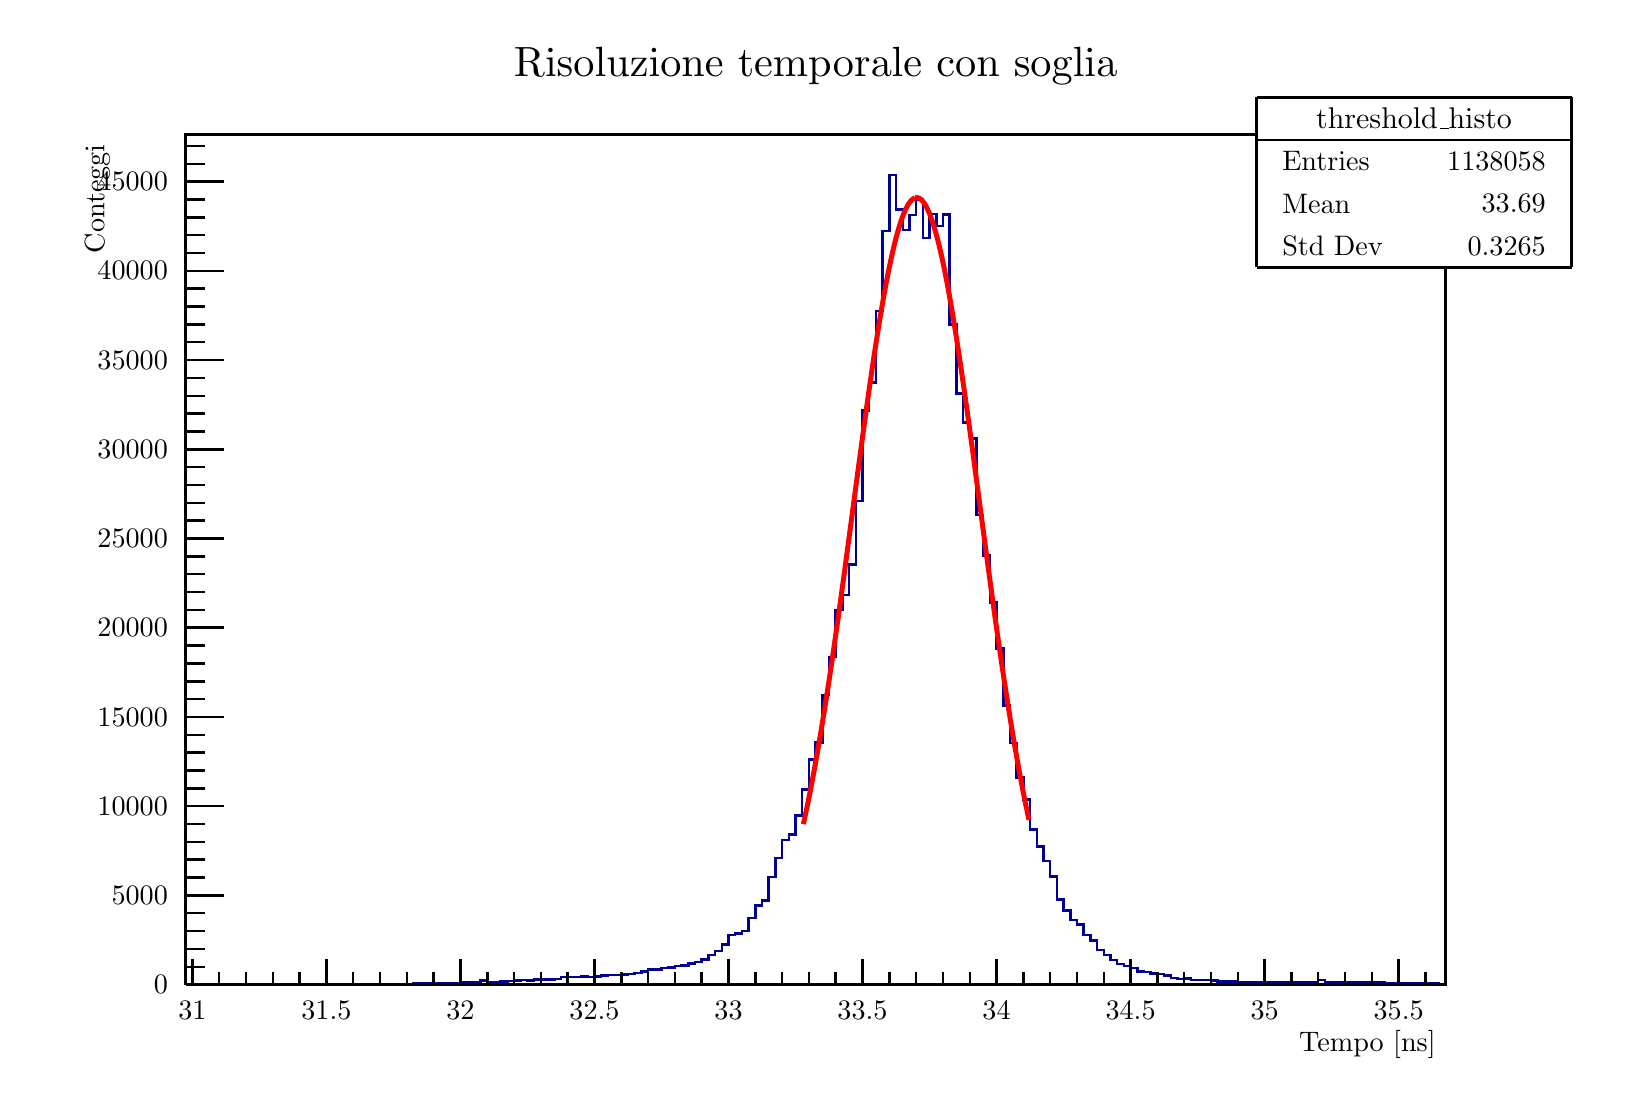
\begin{tikzpicture}
\pgfdeclareplotmark{cross} {
\pgfpathmoveto{\pgfpoint{-0.3\pgfplotmarksize}{\pgfplotmarksize}}
\pgfpathlineto{\pgfpoint{+0.3\pgfplotmarksize}{\pgfplotmarksize}}
\pgfpathlineto{\pgfpoint{+0.3\pgfplotmarksize}{0.3\pgfplotmarksize}}
\pgfpathlineto{\pgfpoint{+1\pgfplotmarksize}{0.3\pgfplotmarksize}}
\pgfpathlineto{\pgfpoint{+1\pgfplotmarksize}{-0.3\pgfplotmarksize}}
\pgfpathlineto{\pgfpoint{+0.3\pgfplotmarksize}{-0.3\pgfplotmarksize}}
\pgfpathlineto{\pgfpoint{+0.3\pgfplotmarksize}{-1.\pgfplotmarksize}}
\pgfpathlineto{\pgfpoint{-0.3\pgfplotmarksize}{-1.\pgfplotmarksize}}
\pgfpathlineto{\pgfpoint{-0.3\pgfplotmarksize}{-0.3\pgfplotmarksize}}
\pgfpathlineto{\pgfpoint{-1.\pgfplotmarksize}{-0.3\pgfplotmarksize}}
\pgfpathlineto{\pgfpoint{-1.\pgfplotmarksize}{0.3\pgfplotmarksize}}
\pgfpathlineto{\pgfpoint{-0.3\pgfplotmarksize}{0.3\pgfplotmarksize}}
\pgfpathclose
\pgfusepathqstroke
}
\pgfdeclareplotmark{cross*} {
\pgfpathmoveto{\pgfpoint{-0.3\pgfplotmarksize}{\pgfplotmarksize}}
\pgfpathlineto{\pgfpoint{+0.3\pgfplotmarksize}{\pgfplotmarksize}}
\pgfpathlineto{\pgfpoint{+0.3\pgfplotmarksize}{0.3\pgfplotmarksize}}
\pgfpathlineto{\pgfpoint{+1\pgfplotmarksize}{0.3\pgfplotmarksize}}
\pgfpathlineto{\pgfpoint{+1\pgfplotmarksize}{-0.3\pgfplotmarksize}}
\pgfpathlineto{\pgfpoint{+0.3\pgfplotmarksize}{-0.3\pgfplotmarksize}}
\pgfpathlineto{\pgfpoint{+0.3\pgfplotmarksize}{-1.\pgfplotmarksize}}
\pgfpathlineto{\pgfpoint{-0.3\pgfplotmarksize}{-1.\pgfplotmarksize}}
\pgfpathlineto{\pgfpoint{-0.3\pgfplotmarksize}{-0.3\pgfplotmarksize}}
\pgfpathlineto{\pgfpoint{-1.\pgfplotmarksize}{-0.3\pgfplotmarksize}}
\pgfpathlineto{\pgfpoint{-1.\pgfplotmarksize}{0.3\pgfplotmarksize}}
\pgfpathlineto{\pgfpoint{-0.3\pgfplotmarksize}{0.3\pgfplotmarksize}}
\pgfpathclose
\pgfusepathqfillstroke
}
\pgfdeclareplotmark{newstar} {
\pgfpathmoveto{\pgfqpoint{0pt}{\pgfplotmarksize}}
\pgfpathlineto{\pgfqpointpolar{44}{0.5\pgfplotmarksize}}
\pgfpathlineto{\pgfqpointpolar{18}{\pgfplotmarksize}}
\pgfpathlineto{\pgfqpointpolar{-20}{0.5\pgfplotmarksize}}
\pgfpathlineto{\pgfqpointpolar{-54}{\pgfplotmarksize}}
\pgfpathlineto{\pgfqpointpolar{-90}{0.5\pgfplotmarksize}}
\pgfpathlineto{\pgfqpointpolar{234}{\pgfplotmarksize}}
\pgfpathlineto{\pgfqpointpolar{198}{0.5\pgfplotmarksize}}
\pgfpathlineto{\pgfqpointpolar{162}{\pgfplotmarksize}}
\pgfpathlineto{\pgfqpointpolar{134}{0.5\pgfplotmarksize}}
\pgfpathclose
\pgfusepathqstroke
}
\pgfdeclareplotmark{newstar*} {
\pgfpathmoveto{\pgfqpoint{0pt}{\pgfplotmarksize}}
\pgfpathlineto{\pgfqpointpolar{44}{0.5\pgfplotmarksize}}
\pgfpathlineto{\pgfqpointpolar{18}{\pgfplotmarksize}}
\pgfpathlineto{\pgfqpointpolar{-20}{0.5\pgfplotmarksize}}
\pgfpathlineto{\pgfqpointpolar{-54}{\pgfplotmarksize}}
\pgfpathlineto{\pgfqpointpolar{-90}{0.5\pgfplotmarksize}}
\pgfpathlineto{\pgfqpointpolar{234}{\pgfplotmarksize}}
\pgfpathlineto{\pgfqpointpolar{198}{0.5\pgfplotmarksize}}
\pgfpathlineto{\pgfqpointpolar{162}{\pgfplotmarksize}}
\pgfpathlineto{\pgfqpointpolar{134}{0.5\pgfplotmarksize}}
\pgfpathclose
\pgfusepathqfillstroke
}
\definecolor{c}{rgb}{1,1,1};
\draw [color=c, fill=c] (0,0) rectangle (20,13.4957);
\draw [color=c, fill=c] (2,1.34957) rectangle (18,12.1461);
\definecolor{c}{rgb}{0,0,0};
\draw [c,line width=0.9] (2,1.34957) -- (2,12.1461) -- (18,12.1461) -- (18,1.34957) -- (2,1.34957);
\definecolor{c}{rgb}{1,1,1};
\draw [color=c, fill=c] (2,1.34957) rectangle (18,12.1461);
\definecolor{c}{rgb}{0,0,0};
\draw [c,line width=0.9] (2,1.34957) -- (2,12.1461) -- (18,12.1461) -- (18,1.34957) -- (2,1.34957);
\definecolor{c}{rgb}{0,0,0.6};
\draw [c,line width=0.9] (2,1.35569) -- (2.08511,1.35569) -- (2.08511,1.35614) -- (2.17021,1.35614) -- (2.17021,1.3566) -- (2.25532,1.3566) -- (2.25532,1.35592) -- (2.34043,1.35592) -- (2.34043,1.35546) -- (2.42553,1.35546) -- (2.42553,1.35682) --
 (2.51064,1.35682) -- (2.51064,1.35546) -- (2.59574,1.35546) -- (2.59574,1.35705) -- (2.68085,1.35705) -- (2.68085,1.3566) -- (2.76596,1.3566) -- (2.76596,1.35433) -- (2.85106,1.35433) -- (2.85106,1.35614) -- (2.93617,1.35614) -- (2.93617,1.35592) --
 (3.02128,1.35592) -- (3.02128,1.35501) -- (3.10638,1.35501) -- (3.10638,1.35478) -- (3.19149,1.35478) -- (3.19149,1.35501) -- (3.2766,1.35501) -- (3.2766,1.35342) -- (3.3617,1.35342) -- (3.3617,1.35478) -- (3.44681,1.35478) -- (3.44681,1.35546) --
 (3.53191,1.35546) -- (3.53191,1.3532) -- (3.61702,1.3532) -- (3.61702,1.35637) -- (3.70213,1.35637) -- (3.70213,1.3566) -- (3.78723,1.3566) -- (3.78723,1.35365) -- (3.87234,1.35365) -- (3.87234,1.35342) -- (3.95745,1.35342) -- (3.95745,1.35501) --
 (4.04255,1.35501) -- (4.04255,1.35388) -- (4.12766,1.35388) -- (4.12766,1.35614) -- (4.21277,1.35614) -- (4.21277,1.35569) -- (4.29787,1.35569) -- (4.29787,1.35705) -- (4.38298,1.35705) -- (4.38298,1.35546) -- (4.46809,1.35546) -- (4.46809,1.35637)
 -- (4.55319,1.35637) -- (4.55319,1.35705) -- (4.6383,1.35705) -- (4.6383,1.35795) -- (4.7234,1.35795) -- (4.7234,1.35931) -- (4.80851,1.35931) -- (4.80851,1.36022) -- (4.89362,1.36022) -- (4.89362,1.36317) -- (4.97872,1.36317) -- (4.97872,1.3609) --
 (5.06383,1.3609) -- (5.06383,1.36317) -- (5.14894,1.36317) -- (5.14894,1.36362) -- (5.23404,1.36362) -- (5.23404,1.37087) -- (5.31915,1.37087) -- (5.31915,1.36566) -- (5.40426,1.36566) -- (5.40426,1.37042) -- (5.48936,1.37042) -- (5.48936,1.37336)
 -- (5.57447,1.37336) -- (5.57447,1.37586) -- (5.65957,1.37586) -- (5.65957,1.37382) -- (5.74468,1.37382) -- (5.74468,1.40282) -- (5.82979,1.40282) -- (5.82979,1.37948) -- (5.91489,1.37948) -- (5.91489,1.38424) -- (6,1.38424) -- (6,1.38855) --
 (6.08511,1.38855) -- (6.08511,1.39784) -- (6.17021,1.39784) -- (6.17021,1.40396) -- (6.25532,1.40396) -- (6.25532,1.40622) -- (6.34043,1.40622) -- (6.34043,1.40441) -- (6.42553,1.40441) -- (6.42553,1.4162) -- (6.51064,1.4162) -- (6.51064,1.41665) --
 (6.59574,1.41665) -- (6.59574,1.41574) -- (6.68085,1.41574) -- (6.68085,1.42367) -- (6.76596,1.42367) -- (6.76596,1.44792) -- (6.85106,1.44792) -- (6.85106,1.44747) -- (6.93617,1.44747) -- (6.93617,1.44498) -- (7.02128,1.44498) -- (7.02128,1.452) --
 (7.10638,1.452) -- (7.10638,1.44724) -- (7.19149,1.44724) -- (7.19149,1.45381) -- (7.2766,1.45381) -- (7.2766,1.46492) -- (7.3617,1.46492) -- (7.3617,1.47353) -- (7.44681,1.47353) -- (7.44681,1.47262) -- (7.53191,1.47262) -- (7.53191,1.48055) --
 (7.61702,1.48055) -- (7.61702,1.48577) -- (7.70213,1.48577) -- (7.70213,1.49959) -- (7.78723,1.49959) -- (7.78723,1.51432) -- (7.87234,1.51432) -- (7.87234,1.54355) -- (7.95745,1.54355) -- (7.95745,1.54151) -- (8.04255,1.54151) -- (8.04255,1.56304)
 -- (8.12766,1.56304) -- (8.12766,1.56644) -- (8.21277,1.56644) -- (8.21277,1.58616) -- (8.29787,1.58616) -- (8.29787,1.59499) -- (8.38298,1.59499) -- (8.38298,1.61856) -- (8.46809,1.61856) -- (8.46809,1.63805) -- (8.55319,1.63805) -- (8.55319,1.67)
 -- (8.6383,1.67) -- (8.6383,1.72734) -- (8.7234,1.72734) -- (8.7234,1.7781) -- (8.80851,1.7781) -- (8.80851,1.85968) -- (8.89362,1.85968) -- (8.89362,1.97729) -- (8.97872,1.97729) -- (8.97872,2.00177) -- (9.06383,2.00177) -- (9.06383,2.03259) --
 (9.14894,2.03259) -- (9.14894,2.19666) -- (9.23404,2.19666) -- (9.23404,2.35484) -- (9.31915,2.35484) -- (9.31915,2.41625) -- (9.40425,2.41625) -- (9.40425,2.71742) -- (9.48936,2.71742) -- (9.48936,2.95559) -- (9.57447,2.95559) -- (9.57447,3.18742)
 -- (9.65957,3.18742) -- (9.65957,3.25427) -- (9.74468,3.25427) -- (9.74468,3.49834) -- (9.82979,3.49834) -- (9.82979,3.82511) -- (9.91489,3.82511) -- (9.91489,4.2056) -- (10,4.2056) -- (10,4.42474) -- (10.0851,4.42474) -- (10.0851,5.0264) --
 (10.1702,5.0264) -- (10.1702,5.51249) -- (10.2553,5.51249) -- (10.2553,6.10396) -- (10.3404,6.10396) -- (10.3404,6.29771) -- (10.4255,6.29771) -- (10.4255,6.68409) -- (10.5106,6.68409) -- (10.5106,7.49334) -- (10.5957,7.49334) -- (10.5957,8.63842)
 -- (10.6809,8.63842) -- (10.6809,8.99919) -- (10.766,8.99919) -- (10.766,9.90429) -- (10.8511,9.90429) -- (10.8511,10.9193) -- (10.9362,10.9193) -- (10.9362,11.632) -- (11.0213,11.632) -- (11.0213,11.1906) -- (11.1064,11.1906) -- (11.1064,10.9336)
 -- (11.1915,10.9336) -- (11.1915,11.1251) -- (11.2766,11.1251) -- (11.2766,11.3209) -- (11.3617,11.3209) -- (11.3617,10.8298) -- (11.4468,10.8298) -- (11.4468,11.1391) -- (11.5319,11.1391) -- (11.5319,10.9862) -- (11.617,10.9862) -- (11.617,11.133)
 -- (11.7021,11.133) -- (11.7021,9.73184) -- (11.7872,9.73184) -- (11.7872,8.85711) -- (11.8723,8.85711) -- (11.8723,8.48523) -- (11.9574,8.48523) -- (11.9574,8.28785) -- (12.0426,8.28785) -- (12.0426,7.31522) -- (12.1277,7.31522) --
 (12.1277,6.79808) -- (12.2128,6.79808) -- (12.2128,6.20231) -- (12.2979,6.20231) -- (12.2979,5.61809) -- (12.383,5.61809) -- (12.383,4.89633) -- (12.4681,4.89633) -- (12.4681,4.4159) -- (12.5532,4.4159) -- (12.5532,3.98216) -- (12.6383,3.98216) --
 (12.6383,3.70138) -- (12.7234,3.70138) -- (12.7234,3.31976) -- (12.8085,3.31976) -- (12.8085,3.10357) -- (12.8936,3.10357) -- (12.8936,2.92251) -- (12.9787,2.92251) -- (12.9787,2.72218) -- (13.0638,2.72218) -- (13.0638,2.43279) -- (13.1489,2.43279)
 -- (13.1489,2.28866) -- (13.234,2.28866) -- (13.234,2.16697) -- (13.3191,2.16697) -- (13.3191,2.11009) -- (13.4043,2.11009) -- (13.4043,1.98228) -- (13.4894,1.98228) -- (13.4894,1.90704) -- (13.5745,1.90704) -- (13.5745,1.78988) -- (13.6596,1.78988)
 -- (13.6596,1.72575) -- (13.7447,1.72575) -- (13.7447,1.66003) -- (13.8298,1.66003) -- (13.8298,1.6129) -- (13.9149,1.6129) -- (13.9149,1.58344) -- (14,1.58344) -- (14,1.55942) -- (14.0851,1.55942) -- (14.0851,1.51568) -- (14.1702,1.51568) --
 (14.1702,1.51137) -- (14.2553,1.51137) -- (14.2553,1.49166) -- (14.3404,1.49166) -- (14.3404,1.4835) -- (14.4255,1.4835) -- (14.4255,1.46378) -- (14.5106,1.46378) -- (14.5106,1.43093) -- (14.5957,1.43093) -- (14.5957,1.42186) -- (14.6809,1.42186) --
 (14.6809,1.42707) -- (14.766,1.42707) -- (14.766,1.4103) -- (14.8511,1.4103) -- (14.8511,1.41008) -- (14.9362,1.41008) -- (14.9362,1.40894) -- (15.0213,1.40894) -- (15.0213,1.39875) -- (15.1064,1.39875) -- (15.1064,1.39172) -- (15.1915,1.39172) --
 (15.1915,1.38923) -- (15.2766,1.38923) -- (15.2766,1.38855) -- (15.3617,1.38855) -- (15.3617,1.38198) -- (15.4468,1.38198) -- (15.4468,1.37948) -- (15.5319,1.37948) -- (15.5319,1.38152) -- (15.617,1.38152) -- (15.617,1.37812) -- (15.7021,1.37812) --
 (15.7021,1.38311) -- (15.7872,1.38311) -- (15.7872,1.37767) -- (15.8723,1.37767) -- (15.8723,1.37382) -- (15.9574,1.37382) -- (15.9574,1.37654) -- (16.0426,1.37654) -- (16.0426,1.37563) -- (16.1277,1.37563) -- (16.1277,1.37563) -- (16.2128,1.37563)
 -- (16.2128,1.37722) -- (16.2979,1.37722) -- (16.2979,1.37948) -- (16.383,1.37948) -- (16.383,1.40804) -- (16.4681,1.40804) -- (16.4681,1.3788) -- (16.5532,1.3788) -- (16.5532,1.37563) -- (16.6383,1.37563) -- (16.6383,1.37835) -- (16.7234,1.37835)
 -- (16.7234,1.37563) -- (16.8085,1.37563) -- (16.8085,1.37926) -- (16.8936,1.37926) -- (16.8936,1.38084) -- (16.9787,1.38084) -- (16.9787,1.37971) -- (17.0638,1.37971) -- (17.0638,1.37427) -- (17.1489,1.37427) -- (17.1489,1.37676) --
 (17.234,1.37676) -- (17.234,1.3711) -- (17.3191,1.3711) -- (17.3191,1.37155) -- (17.4043,1.37155) -- (17.4043,1.36725) -- (17.4894,1.36725) -- (17.4894,1.36951) -- (17.5745,1.36951) -- (17.5745,1.37065) -- (17.6596,1.37065) -- (17.6596,1.36249) --
 (17.7447,1.36249) -- (17.7447,1.36566) -- (17.8298,1.36566) -- (17.8298,1.3609) -- (17.9149,1.3609) -- (17.9149,1.35818) -- (18,1.35818);
\definecolor{c}{rgb}{1,1,1};
\draw [color=c, fill=c] (15.6,10.4592) rectangle (19.6,12.6185);
\definecolor{c}{rgb}{0,0,0};
\draw [c,line width=0.9] (15.6,10.4592) -- (19.6,10.4592);
\draw [c,line width=0.9] (19.6,10.4592) -- (19.6,12.6185);
\draw [c,line width=0.9] (19.6,12.6185) -- (15.6,12.6185);
\draw [c,line width=0.9] (15.6,12.6185) -- (15.6,10.4592);
\draw (17.6,12.3486) node[scale=1.08185, color=c, rotate=0]{threshold\_histo};
\draw [c,line width=0.9] (15.6,12.0787) -- (19.6,12.0787);
\draw [anchor= west] (15.8,11.8087) node[scale=1.01821, color=c, rotate=0]{Entries };
\draw [anchor= east] (19.4,11.8087) node[scale=1.01821, color=c, rotate=0]{ 1138058};
\draw [anchor= west] (15.8,11.2689) node[scale=1.01821, color=c, rotate=0]{Mean  };
\draw [anchor= east] (19.4,11.2689) node[scale=1.01821, color=c, rotate=0]{  33.69};
\draw [anchor= west] (15.8,10.7291) node[scale=1.01821, color=c, rotate=0]{Std Dev   };
\draw [anchor= east] (19.4,10.7291) node[scale=1.01821, color=c, rotate=0]{ 0.3265};
\definecolor{c}{rgb}{1,0,0};
\draw [c,line width=1.8] (9.84426,3.38797) -- (9.87319,3.52123) -- (9.90213,3.66022) -- (9.93106,3.80495) -- (9.96,3.95539) -- (9.98894,4.11149) -- (10.0179,4.27318) -- (10.0468,4.44035) -- (10.0757,4.61288) -- (10.1047,4.79061) -- (10.1336,4.97336)
 -- (10.1626,5.1609) -- (10.1915,5.35299) -- (10.2204,5.54935) -- (10.2494,5.74968) -- (10.2783,5.95363) -- (10.3072,6.16085) -- (10.3362,6.37092) -- (10.3651,6.58343) -- (10.394,6.79792) -- (10.423,7.0139) -- (10.4519,7.23087) -- (10.4809,7.44829)
 -- (10.5098,7.66562) -- (10.5387,7.88229) -- (10.5677,8.0977) -- (10.5966,8.31124) -- (10.6255,8.52231) -- (10.6545,8.73027) -- (10.6834,8.93449) -- (10.7123,9.13435) -- (10.7413,9.32919) -- (10.7702,9.51839) -- (10.7991,9.70132) --
 (10.8281,9.87736) -- (10.857,10.0459) -- (10.886,10.2064) -- (10.9149,10.3583) -- (10.9438,10.5009) -- (10.9728,10.6339) -- (11.0017,10.7567) -- (11.0306,10.8688) -- (11.0596,10.9699) -- (11.0885,11.0596) -- (11.1174,11.1375) -- (11.1464,11.2034) --
 (11.1753,11.2569) -- (11.2043,11.2979) -- (11.2332,11.3262) -- (11.2621,11.3418);
\draw [c,line width=1.8] (11.2621,11.3418) -- (11.2911,11.3445) -- (11.32,11.3343) -- (11.3489,11.3113) -- (11.3779,11.2756) -- (11.4068,11.2273) -- (11.4357,11.1666) -- (11.4647,11.0938) -- (11.4936,11.009) -- (11.5226,10.9126) -- (11.5515,10.8051)
 -- (11.5804,10.6867) -- (11.6094,10.5579) -- (11.6383,10.4193) -- (11.6672,10.2712) -- (11.6962,10.1143) -- (11.7251,9.94904) -- (11.754,9.77606) -- (11.783,9.59595) -- (11.8119,9.4093) -- (11.8409,9.21675) -- (11.8698,9.01893) -- (11.8987,8.81646)
 -- (11.9277,8.60999) -- (11.9566,8.40015) -- (11.9855,8.18757) -- (12.0145,7.97287) -- (12.0434,7.75666) -- (12.0723,7.53954) -- (12.1013,7.32208) -- (12.1302,7.10485) -- (12.1591,6.88839) -- (12.1881,6.67322) -- (12.217,6.45983) -- (12.246,6.24868)
 -- (12.2749,6.04021) -- (12.3038,5.83484) -- (12.3328,5.63295) -- (12.3617,5.43488) -- (12.3906,5.24096) -- (12.4196,5.05148) -- (12.4485,4.8667) -- (12.4774,4.68684) -- (12.5064,4.51211) -- (12.5353,4.34267) -- (12.5643,4.17867) --
 (12.5932,4.02021) -- (12.6221,3.86739) -- (12.6511,3.72026) -- (12.68,3.57886);
\draw [c,line width=1.8] (12.68,3.57886) -- (12.7089,3.44319);
\definecolor{c}{rgb}{0,0,0};
\draw [c,line width=0.9] (2,1.34957) -- (18,1.34957);
\draw [anchor= east] (18,0.593811) node[scale=1.01821, color=c, rotate=0]{Tempo [ns]};
\draw [c,line width=0.9] (2.08511,1.67347) -- (2.08511,1.34957);
\draw [c,line width=0.9] (2.42553,1.51152) -- (2.42553,1.34957);
\draw [c,line width=0.9] (2.76596,1.51152) -- (2.76596,1.34957);
\draw [c,line width=0.9] (3.10638,1.51152) -- (3.10638,1.34957);
\draw [c,line width=0.9] (3.44681,1.51152) -- (3.44681,1.34957);
\draw [c,line width=0.9] (3.78723,1.67347) -- (3.78723,1.34957);
\draw [c,line width=0.9] (4.12766,1.51152) -- (4.12766,1.34957);
\draw [c,line width=0.9] (4.46809,1.51152) -- (4.46809,1.34957);
\draw [c,line width=0.9] (4.80851,1.51152) -- (4.80851,1.34957);
\draw [c,line width=0.9] (5.14894,1.51152) -- (5.14894,1.34957);
\draw [c,line width=0.9] (5.48936,1.67347) -- (5.48936,1.34957);
\draw [c,line width=0.9] (5.82979,1.51152) -- (5.82979,1.34957);
\draw [c,line width=0.9] (6.17021,1.51152) -- (6.17021,1.34957);
\draw [c,line width=0.9] (6.51064,1.51152) -- (6.51064,1.34957);
\draw [c,line width=0.9] (6.85106,1.51152) -- (6.85106,1.34957);
\draw [c,line width=0.9] (7.19149,1.67347) -- (7.19149,1.34957);
\draw [c,line width=0.9] (7.53191,1.51152) -- (7.53191,1.34957);
\draw [c,line width=0.9] (7.87234,1.51152) -- (7.87234,1.34957);
\draw [c,line width=0.9] (8.21277,1.51152) -- (8.21277,1.34957);
\draw [c,line width=0.9] (8.55319,1.51152) -- (8.55319,1.34957);
\draw [c,line width=0.9] (8.89362,1.67347) -- (8.89362,1.34957);
\draw [c,line width=0.9] (9.23404,1.51152) -- (9.23404,1.34957);
\draw [c,line width=0.9] (9.57447,1.51152) -- (9.57447,1.34957);
\draw [c,line width=0.9] (9.91489,1.51152) -- (9.91489,1.34957);
\draw [c,line width=0.9] (10.2553,1.51152) -- (10.2553,1.34957);
\draw [c,line width=0.9] (10.5957,1.67347) -- (10.5957,1.34957);
\draw [c,line width=0.9] (10.9362,1.51152) -- (10.9362,1.34957);
\draw [c,line width=0.9] (11.2766,1.51152) -- (11.2766,1.34957);
\draw [c,line width=0.9] (11.617,1.51152) -- (11.617,1.34957);
\draw [c,line width=0.9] (11.9574,1.51152) -- (11.9574,1.34957);
\draw [c,line width=0.9] (12.2979,1.67347) -- (12.2979,1.34957);
\draw [c,line width=0.9] (12.6383,1.51152) -- (12.6383,1.34957);
\draw [c,line width=0.9] (12.9787,1.51152) -- (12.9787,1.34957);
\draw [c,line width=0.9] (13.3191,1.51152) -- (13.3191,1.34957);
\draw [c,line width=0.9] (13.6596,1.51152) -- (13.6596,1.34957);
\draw [c,line width=0.9] (14,1.67347) -- (14,1.34957);
\draw [c,line width=0.9] (14.3404,1.51152) -- (14.3404,1.34957);
\draw [c,line width=0.9] (14.6809,1.51152) -- (14.6809,1.34957);
\draw [c,line width=0.9] (15.0213,1.51152) -- (15.0213,1.34957);
\draw [c,line width=0.9] (15.3617,1.51152) -- (15.3617,1.34957);
\draw [c,line width=0.9] (15.7021,1.67347) -- (15.7021,1.34957);
\draw [c,line width=0.9] (16.0426,1.51152) -- (16.0426,1.34957);
\draw [c,line width=0.9] (16.383,1.51152) -- (16.383,1.34957);
\draw [c,line width=0.9] (16.7234,1.51152) -- (16.7234,1.34957);
\draw [c,line width=0.9] (17.0638,1.51152) -- (17.0638,1.34957);
\draw [c,line width=0.9] (17.4043,1.67347) -- (17.4043,1.34957);
\draw [c,line width=0.9] (2.08511,1.67347) -- (2.08511,1.34957);
\draw [c,line width=0.9] (17.4043,1.67347) -- (17.4043,1.34957);
\draw [c,line width=0.9] (17.7447,1.51152) -- (17.7447,1.34957);
\draw [anchor=base] (2.08511,0.904212) node[scale=1.01821, color=c, rotate=0]{31};
\draw [anchor=base] (3.78723,0.904212) node[scale=1.01821, color=c, rotate=0]{31.5};
\draw [anchor=base] (5.48936,0.904212) node[scale=1.01821, color=c, rotate=0]{32};
\draw [anchor=base] (7.19149,0.904212) node[scale=1.01821, color=c, rotate=0]{32.5};
\draw [anchor=base] (8.89362,0.904212) node[scale=1.01821, color=c, rotate=0]{33};
\draw [anchor=base] (10.5957,0.904212) node[scale=1.01821, color=c, rotate=0]{33.5};
\draw [anchor=base] (12.2979,0.904212) node[scale=1.01821, color=c, rotate=0]{34};
\draw [anchor=base] (14,0.904212) node[scale=1.01821, color=c, rotate=0]{34.5};
\draw [anchor=base] (15.7021,0.904212) node[scale=1.01821, color=c, rotate=0]{35};
\draw [anchor=base] (17.4043,0.904212) node[scale=1.01821, color=c, rotate=0]{35.5};
\draw [c,line width=0.9] (2,1.34957) -- (2,12.1461);
\draw [anchor= east] (0.88,12.1461) node[scale=1.01821, color=c, rotate=90]{Conteggi};
\draw [c,line width=0.9] (2.48,1.34957) -- (2,1.34957);
\draw [c,line width=0.9] (2.24,1.57619) -- (2,1.57619);
\draw [c,line width=0.9] (2.24,1.8028) -- (2,1.8028);
\draw [c,line width=0.9] (2.24,2.02942) -- (2,2.02942);
\draw [c,line width=0.9] (2.24,2.25603) -- (2,2.25603);
\draw [c,line width=0.9] (2.48,2.48265) -- (2,2.48265);
\draw [c,line width=0.9] (2.24,2.70926) -- (2,2.70926);
\draw [c,line width=0.9] (2.24,2.93588) -- (2,2.93588);
\draw [c,line width=0.9] (2.24,3.16249) -- (2,3.16249);
\draw [c,line width=0.9] (2.24,3.38911) -- (2,3.38911);
\draw [c,line width=0.9] (2.48,3.61572) -- (2,3.61572);
\draw [c,line width=0.9] (2.24,3.84234) -- (2,3.84234);
\draw [c,line width=0.9] (2.24,4.06895) -- (2,4.06895);
\draw [c,line width=0.9] (2.24,4.29557) -- (2,4.29557);
\draw [c,line width=0.9] (2.24,4.52218) -- (2,4.52218);
\draw [c,line width=0.9] (2.48,4.7488) -- (2,4.7488);
\draw [c,line width=0.9] (2.24,4.97541) -- (2,4.97541);
\draw [c,line width=0.9] (2.24,5.20203) -- (2,5.20203);
\draw [c,line width=0.9] (2.24,5.42864) -- (2,5.42864);
\draw [c,line width=0.9] (2.24,5.65526) -- (2,5.65526);
\draw [c,line width=0.9] (2.48,5.88187) -- (2,5.88187);
\draw [c,line width=0.9] (2.24,6.10849) -- (2,6.10849);
\draw [c,line width=0.9] (2.24,6.33511) -- (2,6.33511);
\draw [c,line width=0.9] (2.24,6.56172) -- (2,6.56172);
\draw [c,line width=0.9] (2.24,6.78834) -- (2,6.78834);
\draw [c,line width=0.9] (2.48,7.01495) -- (2,7.01495);
\draw [c,line width=0.9] (2.24,7.24157) -- (2,7.24157);
\draw [c,line width=0.9] (2.24,7.46818) -- (2,7.46818);
\draw [c,line width=0.9] (2.24,7.6948) -- (2,7.6948);
\draw [c,line width=0.9] (2.24,7.92141) -- (2,7.92141);
\draw [c,line width=0.9] (2.48,8.14803) -- (2,8.14803);
\draw [c,line width=0.9] (2.24,8.37464) -- (2,8.37464);
\draw [c,line width=0.9] (2.24,8.60126) -- (2,8.60126);
\draw [c,line width=0.9] (2.24,8.82787) -- (2,8.82787);
\draw [c,line width=0.9] (2.24,9.05449) -- (2,9.05449);
\draw [c,line width=0.9] (2.48,9.2811) -- (2,9.2811);
\draw [c,line width=0.9] (2.24,9.50772) -- (2,9.50772);
\draw [c,line width=0.9] (2.24,9.73433) -- (2,9.73433);
\draw [c,line width=0.9] (2.24,9.96095) -- (2,9.96095);
\draw [c,line width=0.9] (2.24,10.1876) -- (2,10.1876);
\draw [c,line width=0.9] (2.48,10.4142) -- (2,10.4142);
\draw [c,line width=0.9] (2.24,10.6408) -- (2,10.6408);
\draw [c,line width=0.9] (2.24,10.8674) -- (2,10.8674);
\draw [c,line width=0.9] (2.24,11.094) -- (2,11.094);
\draw [c,line width=0.9] (2.24,11.3206) -- (2,11.3206);
\draw [c,line width=0.9] (2.48,11.5473) -- (2,11.5473);
\draw [c,line width=0.9] (2.48,11.5473) -- (2,11.5473);
\draw [c,line width=0.9] (2.24,11.7739) -- (2,11.7739);
\draw [c,line width=0.9] (2.24,12.0005) -- (2,12.0005);
\draw [anchor= east] (1.9,1.34957) node[scale=1.01821, color=c, rotate=0]{0};
\draw [anchor= east] (1.9,2.48265) node[scale=1.01821, color=c, rotate=0]{5000};
\draw [anchor= east] (1.9,3.61572) node[scale=1.01821, color=c, rotate=0]{10000};
\draw [anchor= east] (1.9,4.7488) node[scale=1.01821, color=c, rotate=0]{15000};
\draw [anchor= east] (1.9,5.88187) node[scale=1.01821, color=c, rotate=0]{20000};
\draw [anchor= east] (1.9,7.01495) node[scale=1.01821, color=c, rotate=0]{25000};
\draw [anchor= east] (1.9,8.14803) node[scale=1.01821, color=c, rotate=0]{30000};
\draw [anchor= east] (1.9,9.2811) node[scale=1.01821, color=c, rotate=0]{35000};
\draw [anchor= east] (1.9,10.4142) node[scale=1.01821, color=c, rotate=0]{40000};
\draw [anchor= east] (1.9,11.5473) node[scale=1.01821, color=c, rotate=0]{45000};
\definecolor{c}{rgb}{1,1,1};
\draw [color=c, fill=c] (15.6,10.4592) rectangle (19.6,12.6185);
\definecolor{c}{rgb}{0,0,0};
\draw [c,line width=0.9] (15.6,10.4592) -- (19.6,10.4592);
\draw [c,line width=0.9] (19.6,10.4592) -- (19.6,12.6185);
\draw [c,line width=0.9] (19.6,12.6185) -- (15.6,12.6185);
\draw [c,line width=0.9] (15.6,12.6185) -- (15.6,10.4592);
\draw (17.6,12.3486) node[scale=1.08185, color=c, rotate=0]{threshold\_histo};
\draw [c,line width=0.9] (15.6,12.0787) -- (19.6,12.0787);
\draw [anchor= west] (15.8,11.8087) node[scale=1.01821, color=c, rotate=0]{Entries };
\draw [anchor= east] (19.4,11.8087) node[scale=1.01821, color=c, rotate=0]{ 1138058};
\draw [anchor= west] (15.8,11.2689) node[scale=1.01821, color=c, rotate=0]{Mean  };
\draw [anchor= east] (19.4,11.2689) node[scale=1.01821, color=c, rotate=0]{  33.69};
\draw [anchor= west] (15.8,10.7291) node[scale=1.01821, color=c, rotate=0]{Std Dev   };
\draw [anchor= east] (19.4,10.7291) node[scale=1.01821, color=c, rotate=0]{ 0.3265};
\draw (10,13.0156) node[scale=1.52731, color=c, rotate=0]{Risoluzione temporale con soglia};
\end{tikzpicture}

%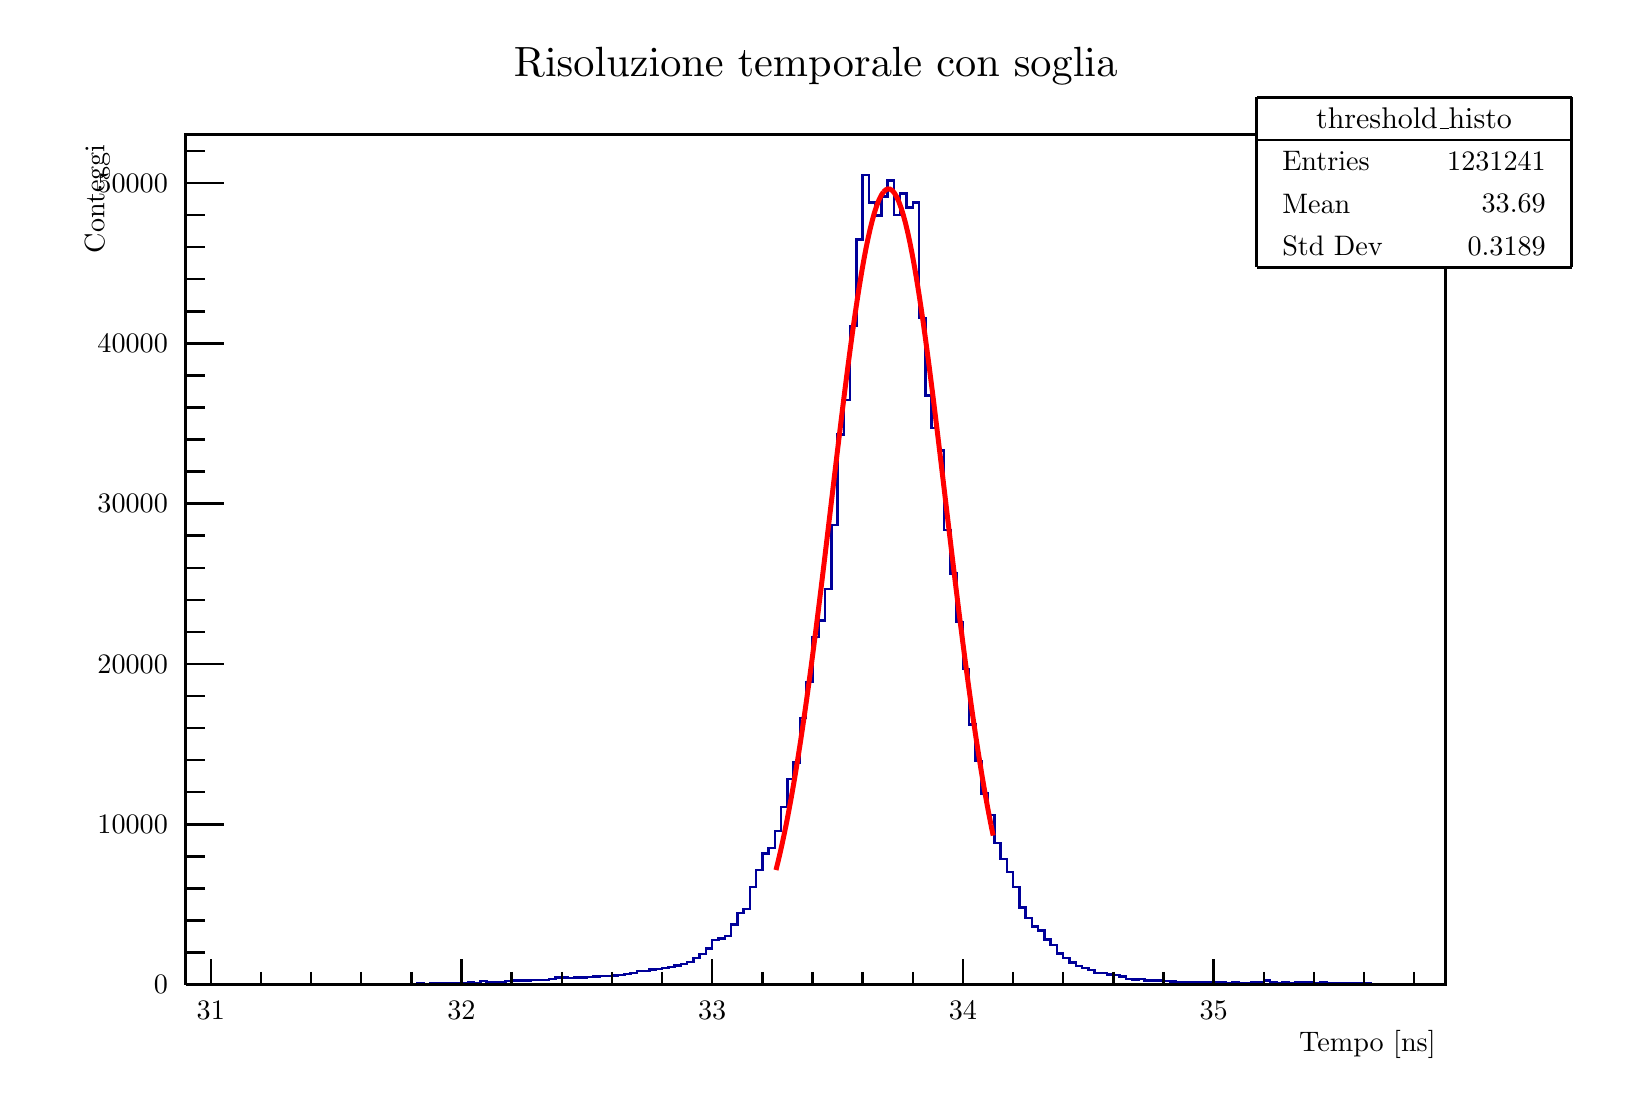
\begin{tikzpicture}
\pgfdeclareplotmark{cross} {
\pgfpathmoveto{\pgfpoint{-0.3\pgfplotmarksize}{\pgfplotmarksize}}
\pgfpathlineto{\pgfpoint{+0.3\pgfplotmarksize}{\pgfplotmarksize}}
\pgfpathlineto{\pgfpoint{+0.3\pgfplotmarksize}{0.3\pgfplotmarksize}}
\pgfpathlineto{\pgfpoint{+1\pgfplotmarksize}{0.3\pgfplotmarksize}}
\pgfpathlineto{\pgfpoint{+1\pgfplotmarksize}{-0.3\pgfplotmarksize}}
\pgfpathlineto{\pgfpoint{+0.3\pgfplotmarksize}{-0.3\pgfplotmarksize}}
\pgfpathlineto{\pgfpoint{+0.3\pgfplotmarksize}{-1.\pgfplotmarksize}}
\pgfpathlineto{\pgfpoint{-0.3\pgfplotmarksize}{-1.\pgfplotmarksize}}
\pgfpathlineto{\pgfpoint{-0.3\pgfplotmarksize}{-0.3\pgfplotmarksize}}
\pgfpathlineto{\pgfpoint{-1.\pgfplotmarksize}{-0.3\pgfplotmarksize}}
\pgfpathlineto{\pgfpoint{-1.\pgfplotmarksize}{0.3\pgfplotmarksize}}
\pgfpathlineto{\pgfpoint{-0.3\pgfplotmarksize}{0.3\pgfplotmarksize}}
\pgfpathclose
\pgfusepathqstroke
}
\pgfdeclareplotmark{cross*} {
\pgfpathmoveto{\pgfpoint{-0.3\pgfplotmarksize}{\pgfplotmarksize}}
\pgfpathlineto{\pgfpoint{+0.3\pgfplotmarksize}{\pgfplotmarksize}}
\pgfpathlineto{\pgfpoint{+0.3\pgfplotmarksize}{0.3\pgfplotmarksize}}
\pgfpathlineto{\pgfpoint{+1\pgfplotmarksize}{0.3\pgfplotmarksize}}
\pgfpathlineto{\pgfpoint{+1\pgfplotmarksize}{-0.3\pgfplotmarksize}}
\pgfpathlineto{\pgfpoint{+0.3\pgfplotmarksize}{-0.3\pgfplotmarksize}}
\pgfpathlineto{\pgfpoint{+0.3\pgfplotmarksize}{-1.\pgfplotmarksize}}
\pgfpathlineto{\pgfpoint{-0.3\pgfplotmarksize}{-1.\pgfplotmarksize}}
\pgfpathlineto{\pgfpoint{-0.3\pgfplotmarksize}{-0.3\pgfplotmarksize}}
\pgfpathlineto{\pgfpoint{-1.\pgfplotmarksize}{-0.3\pgfplotmarksize}}
\pgfpathlineto{\pgfpoint{-1.\pgfplotmarksize}{0.3\pgfplotmarksize}}
\pgfpathlineto{\pgfpoint{-0.3\pgfplotmarksize}{0.3\pgfplotmarksize}}
\pgfpathclose
\pgfusepathqfillstroke
}
\pgfdeclareplotmark{newstar} {
\pgfpathmoveto{\pgfqpoint{0pt}{\pgfplotmarksize}}
\pgfpathlineto{\pgfqpointpolar{44}{0.5\pgfplotmarksize}}
\pgfpathlineto{\pgfqpointpolar{18}{\pgfplotmarksize}}
\pgfpathlineto{\pgfqpointpolar{-20}{0.5\pgfplotmarksize}}
\pgfpathlineto{\pgfqpointpolar{-54}{\pgfplotmarksize}}
\pgfpathlineto{\pgfqpointpolar{-90}{0.5\pgfplotmarksize}}
\pgfpathlineto{\pgfqpointpolar{234}{\pgfplotmarksize}}
\pgfpathlineto{\pgfqpointpolar{198}{0.5\pgfplotmarksize}}
\pgfpathlineto{\pgfqpointpolar{162}{\pgfplotmarksize}}
\pgfpathlineto{\pgfqpointpolar{134}{0.5\pgfplotmarksize}}
\pgfpathclose
\pgfusepathqstroke
}
\pgfdeclareplotmark{newstar*} {
\pgfpathmoveto{\pgfqpoint{0pt}{\pgfplotmarksize}}
\pgfpathlineto{\pgfqpointpolar{44}{0.5\pgfplotmarksize}}
\pgfpathlineto{\pgfqpointpolar{18}{\pgfplotmarksize}}
\pgfpathlineto{\pgfqpointpolar{-20}{0.5\pgfplotmarksize}}
\pgfpathlineto{\pgfqpointpolar{-54}{\pgfplotmarksize}}
\pgfpathlineto{\pgfqpointpolar{-90}{0.5\pgfplotmarksize}}
\pgfpathlineto{\pgfqpointpolar{234}{\pgfplotmarksize}}
\pgfpathlineto{\pgfqpointpolar{198}{0.5\pgfplotmarksize}}
\pgfpathlineto{\pgfqpointpolar{162}{\pgfplotmarksize}}
\pgfpathlineto{\pgfqpointpolar{134}{0.5\pgfplotmarksize}}
\pgfpathclose
\pgfusepathqfillstroke
}
\definecolor{c}{rgb}{1,1,1};
\draw [color=c, fill=c] (0,0) rectangle (20,13.4957);
\draw [color=c, fill=c] (2,1.34957) rectangle (18,12.1461);
\definecolor{c}{rgb}{0,0,0};
\draw [c,line width=0.9] (2,1.34957) -- (2,12.1461) -- (18,12.1461) -- (18,1.34957) -- (2,1.34957);
\definecolor{c}{rgb}{1,1,1};
\draw [color=c, fill=c] (2,1.34957) rectangle (18,12.1461);
\definecolor{c}{rgb}{0,0,0};
\draw [c,line width=0.9] (2,1.34957) -- (2,12.1461) -- (18,12.1461) -- (18,1.34957) -- (2,1.34957);
\definecolor{c}{rgb}{0,0,0.6};
\draw [c,line width=0.9] (2,1.3567) -- (2.0796,1.3567) -- (2.0796,1.35547) -- (2.1592,1.35547) -- (2.1592,1.35486) -- (2.23881,1.35486) -- (2.23881,1.35507) -- (2.31841,1.35507) -- (2.31841,1.35547) -- (2.39801,1.35547) -- (2.39801,1.35588) --
 (2.47761,1.35588) -- (2.47761,1.35527) -- (2.55721,1.35527) -- (2.55721,1.35486) -- (2.63682,1.35486) -- (2.63682,1.35609) -- (2.71642,1.35609) -- (2.71642,1.35486) -- (2.79602,1.35486) -- (2.79602,1.35629) -- (2.87562,1.35629) -- (2.87562,1.35588)
 -- (2.95522,1.35588) -- (2.95522,1.35385) -- (3.03483,1.35385) -- (3.03483,1.35547) -- (3.11443,1.35547) -- (3.11443,1.35547) -- (3.19403,1.35547) -- (3.19403,1.35446) -- (3.27363,1.35446) -- (3.27363,1.35446) -- (3.35323,1.35446) --
 (3.35323,1.35466) -- (3.43284,1.35466) -- (3.43284,1.35303) -- (3.51244,1.35303) -- (3.51244,1.35425) -- (3.59204,1.35425) -- (3.59204,1.35507) -- (3.67164,1.35507) -- (3.67164,1.35303) -- (3.75124,1.35303) -- (3.75124,1.35588) -- (3.83085,1.35588)
 -- (3.83085,1.35609) -- (3.91045,1.35609) -- (3.91045,1.35324) -- (3.99005,1.35324) -- (3.99005,1.35324) -- (4.06965,1.35324) -- (4.06965,1.35466) -- (4.14925,1.35466) -- (4.14925,1.35364) -- (4.22886,1.35364) -- (4.22886,1.35547) --
 (4.30846,1.35547) -- (4.30846,1.35507) -- (4.38806,1.35507) -- (4.38806,1.35629) -- (4.46766,1.35629) -- (4.46766,1.35486) -- (4.54726,1.35486) -- (4.54726,1.35568) -- (4.62687,1.35568) -- (4.62687,1.35629) -- (4.70647,1.35629) -- (4.70647,1.3571)
 -- (4.78607,1.3571) -- (4.78607,1.35853) -- (4.86567,1.35853) -- (4.86567,1.35955) -- (4.94527,1.35955) -- (4.94527,1.36219) -- (5.02488,1.36219) -- (5.02488,1.35995) -- (5.10448,1.35995) -- (5.10448,1.36179) -- (5.18408,1.36179) -- (5.18408,1.3624)
 -- (5.26368,1.3624) -- (5.26368,1.36912) -- (5.34328,1.36912) -- (5.34328,1.36403) -- (5.42289,1.36403) -- (5.42289,1.36851) -- (5.50249,1.36851) -- (5.50249,1.37136) -- (5.58209,1.37136) -- (5.58209,1.3738) -- (5.66169,1.3738) -- (5.66169,1.37176)
 -- (5.74129,1.37176) -- (5.74129,1.39782) -- (5.8209,1.39782) -- (5.8209,1.37645) -- (5.9005,1.37645) -- (5.9005,1.38072) -- (5.9801,1.38072) -- (5.9801,1.3852) -- (6.0597,1.3852) -- (6.0597,1.39335) -- (6.1393,1.39335) -- (6.1393,1.39905) --
 (6.21891,1.39905) -- (6.21891,1.40068) -- (6.29851,1.40068) -- (6.29851,1.39884) -- (6.37811,1.39884) -- (6.37811,1.40963) -- (6.45771,1.40963) -- (6.45771,1.40984) -- (6.53731,1.40984) -- (6.53731,1.40943) -- (6.61692,1.40943) -- (6.61692,1.41798)
 -- (6.69652,1.41798) -- (6.69652,1.43875) -- (6.77612,1.43875) -- (6.77612,1.43773) -- (6.85572,1.43773) -- (6.85572,1.4357) -- (6.93532,1.4357) -- (6.93532,1.44201) -- (7.01493,1.44201) -- (7.01493,1.43814) -- (7.09453,1.43814) -- (7.09453,1.44343)
 -- (7.17413,1.44343) -- (7.17413,1.45341) -- (7.25373,1.45341) -- (7.25373,1.46135) -- (7.33333,1.46135) -- (7.33333,1.46074) -- (7.41294,1.46074) -- (7.41294,1.46766) -- (7.49254,1.46766) -- (7.49254,1.47214) -- (7.57214,1.47214) --
 (7.57214,1.48476) -- (7.65174,1.48476) -- (7.65174,1.49841) -- (7.73134,1.49841) -- (7.73134,1.52426) -- (7.81095,1.52426) -- (7.81095,1.52243) -- (7.89055,1.52243) -- (7.89055,1.54259) -- (7.97015,1.54259) -- (7.97015,1.54483) -- (8.04975,1.54483)
 -- (8.04975,1.56274) -- (8.12935,1.56274) -- (8.12935,1.57028) -- (8.20895,1.57028) -- (8.20895,1.59206) -- (8.28856,1.59206) -- (8.28856,1.60957) -- (8.36816,1.60957) -- (8.36816,1.63889) -- (8.44776,1.63889) -- (8.44776,1.68979) --
 (8.52736,1.68979) -- (8.52736,1.7356) -- (8.60697,1.7356) -- (8.60697,1.80992) -- (8.68657,1.80992) -- (8.68657,1.91559) -- (8.76617,1.91559) -- (8.76617,1.93778) -- (8.84577,1.93778) -- (8.84577,1.96547) -- (8.92537,1.96547) -- (8.92537,2.11411) --
 (9.00498,2.11411) -- (9.00498,2.25643) -- (9.08458,2.25643) -- (9.08458,2.31242) -- (9.16418,2.31242) -- (9.16418,2.58667) -- (9.24378,2.58667) -- (9.24378,2.80473) -- (9.32338,2.80473) -- (9.32338,3.01404) -- (9.40298,3.01404) -- (9.40298,3.08184)
 -- (9.48259,3.08184) -- (9.48259,3.30112) -- (9.56219,3.30112) -- (9.56219,3.60286) -- (9.64179,3.60286) -- (9.64179,3.95978) -- (9.72139,3.95978) -- (9.72139,4.17051) -- (9.80099,4.17051) -- (9.80099,4.73653) -- (9.8806,4.73653) -- (9.8806,5.19159)
 -- (9.9602,5.19159) -- (9.9602,5.76616) -- (10.0398,5.76616) -- (10.0398,5.97078) -- (10.1194,5.97078) -- (10.1194,6.37148) -- (10.199,6.37148) -- (10.199,7.18447) -- (10.2786,7.18447) -- (10.2786,8.33545) -- (10.3582,8.33545) -- (10.3582,8.77564)
 -- (10.4378,8.77564) -- (10.4378,9.71609) -- (10.5174,9.71609) -- (10.5174,10.8154) -- (10.597,10.8154) -- (10.597,11.632) -- (10.6766,11.632) -- (10.6766,11.2824) -- (10.7562,11.2824) -- (10.7562,11.1147) -- (10.8358,11.1147) -- (10.8358,11.361) --
 (10.9154,11.361) -- (10.9154,11.5607) -- (10.995,11.5607) -- (10.995,11.1226) -- (11.0746,11.1226) -- (11.0746,11.3989) -- (11.1542,11.3989) -- (11.1542,11.2207) -- (11.2338,11.2207) -- (11.2338,11.281) -- (11.3134,11.281) -- (11.3134,9.81341) --
 (11.393,9.81341) -- (11.393,8.82878) -- (11.4726,8.82878) -- (11.4726,8.4177) -- (11.5522,8.4177) -- (11.5522,8.13042) -- (11.6318,8.13042) -- (11.6318,7.12319) -- (11.7114,7.12319) -- (11.7114,6.56796) -- (11.791,6.56796) -- (11.791,5.95551) --
 (11.8706,5.95551) -- (11.8706,5.35468) -- (11.9502,5.35468) -- (11.9502,4.65407) -- (12.0299,4.65407) -- (12.0299,4.19087) -- (12.1095,4.19087) -- (12.1095,3.77409) -- (12.1891,3.77409) -- (12.1891,3.50167) -- (12.2687,3.50167) -- (12.2687,3.14638)
 -- (12.3483,3.14638) -- (12.3483,2.94685) -- (12.4279,2.94685) -- (12.4279,2.77765) -- (12.5075,2.77765) -- (12.5075,2.59197) -- (12.5871,2.59197) -- (12.5871,2.32932) -- (12.6667,2.32932) -- (12.6667,2.19636) -- (12.7463,2.19636) --
 (12.7463,2.08682) -- (12.8259,2.08682) -- (12.8259,2.0345) -- (12.9055,2.0345) -- (12.9055,1.92007) -- (12.9851,1.92007) -- (12.9851,1.85146) -- (13.0647,1.85146) -- (13.0647,1.74619) -- (13.1443,1.74619) -- (13.1443,1.68837) -- (13.2239,1.68837) --
 (13.2239,1.62871) -- (13.3035,1.62871) -- (13.3035,1.58616) -- (13.3831,1.58616) -- (13.3831,1.5605) -- (13.4627,1.5605) -- (13.4627,1.53831) -- (13.5423,1.53831) -- (13.5423,1.49881) -- (13.6219,1.49881) -- (13.6219,1.49515) -- (13.7015,1.49515) --
 (13.7015,1.47784) -- (13.7811,1.47784) -- (13.7811,1.47072) -- (13.8607,1.47072) -- (13.8607,1.4528) -- (13.9403,1.4528) -- (13.9403,1.42266) -- (14.0199,1.42266) -- (14.0199,1.41472) -- (14.0995,1.41472) -- (14.0995,1.41941) -- (14.1791,1.41941) --
 (14.1791,1.40414) -- (14.2587,1.40414) -- (14.2587,1.40434) -- (14.3383,1.40434) -- (14.3383,1.40291) -- (14.4179,1.40291) -- (14.4179,1.39396) -- (14.4975,1.39396) -- (14.4975,1.38744) -- (14.5771,1.38744) -- (14.5771,1.3852) -- (14.6567,1.3852) --
 (14.6567,1.38459) -- (14.7363,1.38459) -- (14.7363,1.37889) -- (14.8159,1.37889) -- (14.8159,1.37665) -- (14.8955,1.37665) -- (14.8955,1.37848) -- (14.9751,1.37848) -- (14.9751,1.37543) -- (15.0547,1.37543) -- (15.0547,1.3797) -- (15.1343,1.3797) --
 (15.1343,1.37482) -- (15.2139,1.37482) -- (15.2139,1.37176) -- (15.2935,1.37176) -- (15.2935,1.374) -- (15.3731,1.374) -- (15.3731,1.37298) -- (15.4527,1.37298) -- (15.4527,1.37298) -- (15.5323,1.37298) -- (15.5323,1.37441) -- (15.6119,1.37441) --
 (15.6119,1.37645) -- (15.6915,1.37645) -- (15.6915,1.4021) -- (15.7711,1.4021) -- (15.7711,1.37624) -- (15.8507,1.37624) -- (15.8507,1.37298) -- (15.9303,1.37298) -- (15.9303,1.37543) -- (16.01,1.37543) -- (16.01,1.37298) -- (16.0896,1.37298) --
 (16.0896,1.37645) -- (16.1692,1.37645) -- (16.1692,1.37787) -- (16.2488,1.37787) -- (16.2488,1.37665) -- (16.3284,1.37665) -- (16.3284,1.37176) -- (16.408,1.37176) -- (16.408,1.374) -- (16.4876,1.374) -- (16.4876,1.36912) -- (16.5672,1.36912) --
 (16.5672,1.36932) -- (16.6468,1.36932) -- (16.6468,1.36545) -- (16.7264,1.36545) -- (16.7264,1.36749) -- (16.806,1.36749) -- (16.806,1.36851) -- (16.8856,1.36851) -- (16.8856,1.36118) -- (16.9652,1.36118) -- (16.9652,1.36403) -- (17.0448,1.36403) --
 (17.0448,1.35975) -- (17.1244,1.35975) -- (17.1244,1.35731) -- (17.204,1.35731) -- (17.204,1.35547) -- (17.2836,1.35547) -- (17.2836,1.35649) -- (17.3632,1.35649) -- (17.3632,1.35446) -- (17.4428,1.35446) -- (17.4428,1.35425) -- (17.5224,1.35425) --
 (17.5224,1.35222) -- (17.602,1.35222) -- (17.602,1.35303) -- (17.6816,1.35303) -- (17.6816,1.35242) -- (17.7612,1.35242) -- (17.7612,1.35201) -- (17.8408,1.35201) -- (17.8408,1.3512) -- (17.9204,1.3512) -- (17.9204,1.35079) -- (18,1.35079);
\definecolor{c}{rgb}{1,1,1};
\draw [color=c, fill=c] (15.6,10.4592) rectangle (19.6,12.6185);
\definecolor{c}{rgb}{0,0,0};
\draw [c,line width=0.9] (15.6,10.4592) -- (19.6,10.4592);
\draw [c,line width=0.9] (19.6,10.4592) -- (19.6,12.6185);
\draw [c,line width=0.9] (19.6,12.6185) -- (15.6,12.6185);
\draw [c,line width=0.9] (15.6,12.6185) -- (15.6,10.4592);
\draw (17.6,12.3486) node[scale=1.08185, color=c, rotate=0]{threshold\_histo};
\draw [c,line width=0.9] (15.6,12.0787) -- (19.6,12.0787);
\draw [anchor= west] (15.8,11.8087) node[scale=1.01821, color=c, rotate=0]{Entries };
\draw [anchor= east] (19.4,11.8087) node[scale=1.01821, color=c, rotate=0]{ 1231241};
\draw [anchor= west] (15.8,11.2689) node[scale=1.01821, color=c, rotate=0]{Mean  };
\draw [anchor= east] (19.4,11.2689) node[scale=1.01821, color=c, rotate=0]{  33.69};
\draw [anchor= west] (15.8,10.7291) node[scale=1.01821, color=c, rotate=0]{Std Dev   };
\draw [anchor= east] (19.4,10.7291) node[scale=1.01821, color=c, rotate=0]{ 0.3189};
\definecolor{c}{rgb}{1,0,0};
\draw [c,line width=1.8] (9.49652,2.80454) -- (9.52438,2.91757) -- (9.55224,3.0369) -- (9.5801,3.16264) -- (9.60796,3.29489) -- (9.63582,3.4337) -- (9.66368,3.57914) -- (9.69154,3.73121) -- (9.7194,3.88992) -- (9.74726,4.05521) -- (9.77512,4.22702)
 -- (9.80299,4.40523) -- (9.83085,4.5897) -- (9.85871,4.78026) -- (9.88657,4.97668) -- (9.91443,5.17869) -- (9.94229,5.38602) -- (9.97015,5.5983) -- (9.99801,5.81517) -- (10.0259,6.0362) -- (10.0537,6.26093) -- (10.0816,6.48887) -- (10.1095,6.71947)
 -- (10.1373,6.95216) -- (10.1652,7.18633) -- (10.193,7.42133) -- (10.2209,7.65651) -- (10.2488,7.89115) -- (10.2766,8.12454) -- (10.3045,8.35593) -- (10.3323,8.58456) -- (10.3602,8.80966) -- (10.3881,9.03044) -- (10.4159,9.24611) --
 (10.4438,9.45589) -- (10.4716,9.65901) -- (10.4995,9.85467) -- (10.5274,10.0421) -- (10.5552,10.2207) -- (10.5831,10.3895) -- (10.6109,10.548) -- (10.6388,10.6956) -- (10.6667,10.8315) -- (10.6945,10.9552) -- (10.7224,11.0662) -- (10.7502,11.1641)
 -- (10.7781,11.2483) -- (10.806,11.3186) -- (10.8338,11.3746) -- (10.8617,11.4161);
\draw [c,line width=1.8] (10.8617,11.4161) -- (10.8896,11.4429) -- (10.9174,11.4548) -- (10.9453,11.4519) -- (10.9731,11.4341) -- (11.001,11.4016) -- (11.0289,11.3544) -- (11.0567,11.2927) -- (11.0846,11.2169) -- (11.1124,11.1273) --
 (11.1403,11.0242) -- (11.1682,10.9081) -- (11.196,10.7796) -- (11.2239,10.639) -- (11.2517,10.4871) -- (11.2796,10.3245) -- (11.3075,10.1517) -- (11.3353,9.9696) -- (11.3632,9.77883) -- (11.391,9.58015) -- (11.4189,9.37433) -- (11.4468,9.16214) --
 (11.4746,8.94437) -- (11.5025,8.72181) -- (11.5303,8.49523) -- (11.5582,8.26543) -- (11.5861,8.03316) -- (11.6139,7.79919) -- (11.6418,7.56426) -- (11.6697,7.32906) -- (11.6975,7.09431) -- (11.7254,6.86064) -- (11.7532,6.6287) -- (11.7811,6.39908)
 -- (11.809,6.17234) -- (11.8368,5.94901) -- (11.8647,5.72956) -- (11.8925,5.51444) -- (11.9204,5.30406) -- (11.9483,5.09878) -- (11.9761,4.89892) -- (12.004,4.70478) -- (12.0318,4.51658) -- (12.0597,4.33455) -- (12.0876,4.15883) -- (12.1154,3.98957)
 -- (12.1433,3.82686) -- (12.1711,3.67075) -- (12.199,3.52128) -- (12.2269,3.37845);
\draw [c,line width=1.8] (12.2269,3.37845) -- (12.2547,3.24222);
\definecolor{c}{rgb}{0,0,0};
\draw [c,line width=0.9] (2,1.34957) -- (18,1.34957);
\draw [anchor= east] (18,0.593811) node[scale=1.01821, color=c, rotate=0]{Tempo [ns]};
\draw [c,line width=0.9] (2.31841,1.67347) -- (2.31841,1.34957);
\draw [c,line width=0.9] (2.95522,1.51152) -- (2.95522,1.34957);
\draw [c,line width=0.9] (3.59204,1.51152) -- (3.59204,1.34957);
\draw [c,line width=0.9] (4.22886,1.51152) -- (4.22886,1.34957);
\draw [c,line width=0.9] (4.86567,1.51152) -- (4.86567,1.34957);
\draw [c,line width=0.9] (5.50249,1.67347) -- (5.50249,1.34957);
\draw [c,line width=0.9] (6.1393,1.51152) -- (6.1393,1.34957);
\draw [c,line width=0.9] (6.77612,1.51152) -- (6.77612,1.34957);
\draw [c,line width=0.9] (7.41294,1.51152) -- (7.41294,1.34957);
\draw [c,line width=0.9] (8.04975,1.51152) -- (8.04975,1.34957);
\draw [c,line width=0.9] (8.68657,1.67347) -- (8.68657,1.34957);
\draw [c,line width=0.9] (9.32338,1.51152) -- (9.32338,1.34957);
\draw [c,line width=0.9] (9.9602,1.51152) -- (9.9602,1.34957);
\draw [c,line width=0.9] (10.597,1.51152) -- (10.597,1.34957);
\draw [c,line width=0.9] (11.2338,1.51152) -- (11.2338,1.34957);
\draw [c,line width=0.9] (11.8706,1.67347) -- (11.8706,1.34957);
\draw [c,line width=0.9] (12.5075,1.51152) -- (12.5075,1.34957);
\draw [c,line width=0.9] (13.1443,1.51152) -- (13.1443,1.34957);
\draw [c,line width=0.9] (13.7811,1.51152) -- (13.7811,1.34957);
\draw [c,line width=0.9] (14.4179,1.51152) -- (14.4179,1.34957);
\draw [c,line width=0.9] (15.0547,1.67347) -- (15.0547,1.34957);
\draw [c,line width=0.9] (2.31841,1.67347) -- (2.31841,1.34957);
\draw [c,line width=0.9] (15.0547,1.67347) -- (15.0547,1.34957);
\draw [c,line width=0.9] (15.6915,1.51152) -- (15.6915,1.34957);
\draw [c,line width=0.9] (16.3284,1.51152) -- (16.3284,1.34957);
\draw [c,line width=0.9] (16.9652,1.51152) -- (16.9652,1.34957);
\draw [c,line width=0.9] (17.602,1.51152) -- (17.602,1.34957);
\draw [anchor=base] (2.31841,0.904212) node[scale=1.01821, color=c, rotate=0]{31};
\draw [anchor=base] (5.50249,0.904212) node[scale=1.01821, color=c, rotate=0]{32};
\draw [anchor=base] (8.68657,0.904212) node[scale=1.01821, color=c, rotate=0]{33};
\draw [anchor=base] (11.8706,0.904212) node[scale=1.01821, color=c, rotate=0]{34};
\draw [anchor=base] (15.0547,0.904212) node[scale=1.01821, color=c, rotate=0]{35};
\draw [c,line width=0.9] (2,1.34957) -- (2,12.1461);
\draw [anchor= east] (0.88,12.1461) node[scale=1.01821, color=c, rotate=90]{Conteggi};
\draw [c,line width=0.9] (2.48,1.34957) -- (2,1.34957);
\draw [c,line width=0.9] (2.24,1.75678) -- (2,1.75678);
\draw [c,line width=0.9] (2.24,2.16399) -- (2,2.16399);
\draw [c,line width=0.9] (2.24,2.5712) -- (2,2.5712);
\draw [c,line width=0.9] (2.24,2.97841) -- (2,2.97841);
\draw [c,line width=0.9] (2.48,3.38562) -- (2,3.38562);
\draw [c,line width=0.9] (2.24,3.79283) -- (2,3.79283);
\draw [c,line width=0.9] (2.24,4.20003) -- (2,4.20003);
\draw [c,line width=0.9] (2.24,4.60724) -- (2,4.60724);
\draw [c,line width=0.9] (2.24,5.01445) -- (2,5.01445);
\draw [c,line width=0.9] (2.48,5.42166) -- (2,5.42166);
\draw [c,line width=0.9] (2.24,5.82887) -- (2,5.82887);
\draw [c,line width=0.9] (2.24,6.23608) -- (2,6.23608);
\draw [c,line width=0.9] (2.24,6.64329) -- (2,6.64329);
\draw [c,line width=0.9] (2.24,7.0505) -- (2,7.0505);
\draw [c,line width=0.9] (2.48,7.45771) -- (2,7.45771);
\draw [c,line width=0.9] (2.24,7.86492) -- (2,7.86492);
\draw [c,line width=0.9] (2.24,8.27213) -- (2,8.27213);
\draw [c,line width=0.9] (2.24,8.67934) -- (2,8.67934);
\draw [c,line width=0.9] (2.24,9.08654) -- (2,9.08654);
\draw [c,line width=0.9] (2.48,9.49375) -- (2,9.49375);
\draw [c,line width=0.9] (2.24,9.90096) -- (2,9.90096);
\draw [c,line width=0.9] (2.24,10.3082) -- (2,10.3082);
\draw [c,line width=0.9] (2.24,10.7154) -- (2,10.7154);
\draw [c,line width=0.9] (2.24,11.1226) -- (2,11.1226);
\draw [c,line width=0.9] (2.48,11.5298) -- (2,11.5298);
\draw [c,line width=0.9] (2.48,11.5298) -- (2,11.5298);
\draw [c,line width=0.9] (2.24,11.937) -- (2,11.937);
\draw [anchor= east] (1.9,1.34957) node[scale=1.01821, color=c, rotate=0]{0};
\draw [anchor= east] (1.9,3.38562) node[scale=1.01821, color=c, rotate=0]{10000};
\draw [anchor= east] (1.9,5.42166) node[scale=1.01821, color=c, rotate=0]{20000};
\draw [anchor= east] (1.9,7.45771) node[scale=1.01821, color=c, rotate=0]{30000};
\draw [anchor= east] (1.9,9.49375) node[scale=1.01821, color=c, rotate=0]{40000};
\draw [anchor= east] (1.9,11.5298) node[scale=1.01821, color=c, rotate=0]{50000};
\definecolor{c}{rgb}{1,1,1};
\draw [color=c, fill=c] (15.6,10.4592) rectangle (19.6,12.6185);
\definecolor{c}{rgb}{0,0,0};
\draw [c,line width=0.9] (15.6,10.4592) -- (19.6,10.4592);
\draw [c,line width=0.9] (19.6,10.4592) -- (19.6,12.6185);
\draw [c,line width=0.9] (19.6,12.6185) -- (15.6,12.6185);
\draw [c,line width=0.9] (15.6,12.6185) -- (15.6,10.4592);
\draw (17.6,12.3486) node[scale=1.08185, color=c, rotate=0]{threshold\_histo};
\draw [c,line width=0.9] (15.6,12.0787) -- (19.6,12.0787);
\draw [anchor= west] (15.8,11.8087) node[scale=1.01821, color=c, rotate=0]{Entries };
\draw [anchor= east] (19.4,11.8087) node[scale=1.01821, color=c, rotate=0]{ 1231241};
\draw [anchor= west] (15.8,11.2689) node[scale=1.01821, color=c, rotate=0]{Mean  };
\draw [anchor= east] (19.4,11.2689) node[scale=1.01821, color=c, rotate=0]{  33.69};
\draw [anchor= west] (15.8,10.7291) node[scale=1.01821, color=c, rotate=0]{Std Dev   };
\draw [anchor= east] (19.4,10.7291) node[scale=1.01821, color=c, rotate=0]{ 0.3189};
\draw (10,13.0156) node[scale=1.52731, color=c, rotate=0]{Risoluzione temporale con soglia};
\end{tikzpicture}

%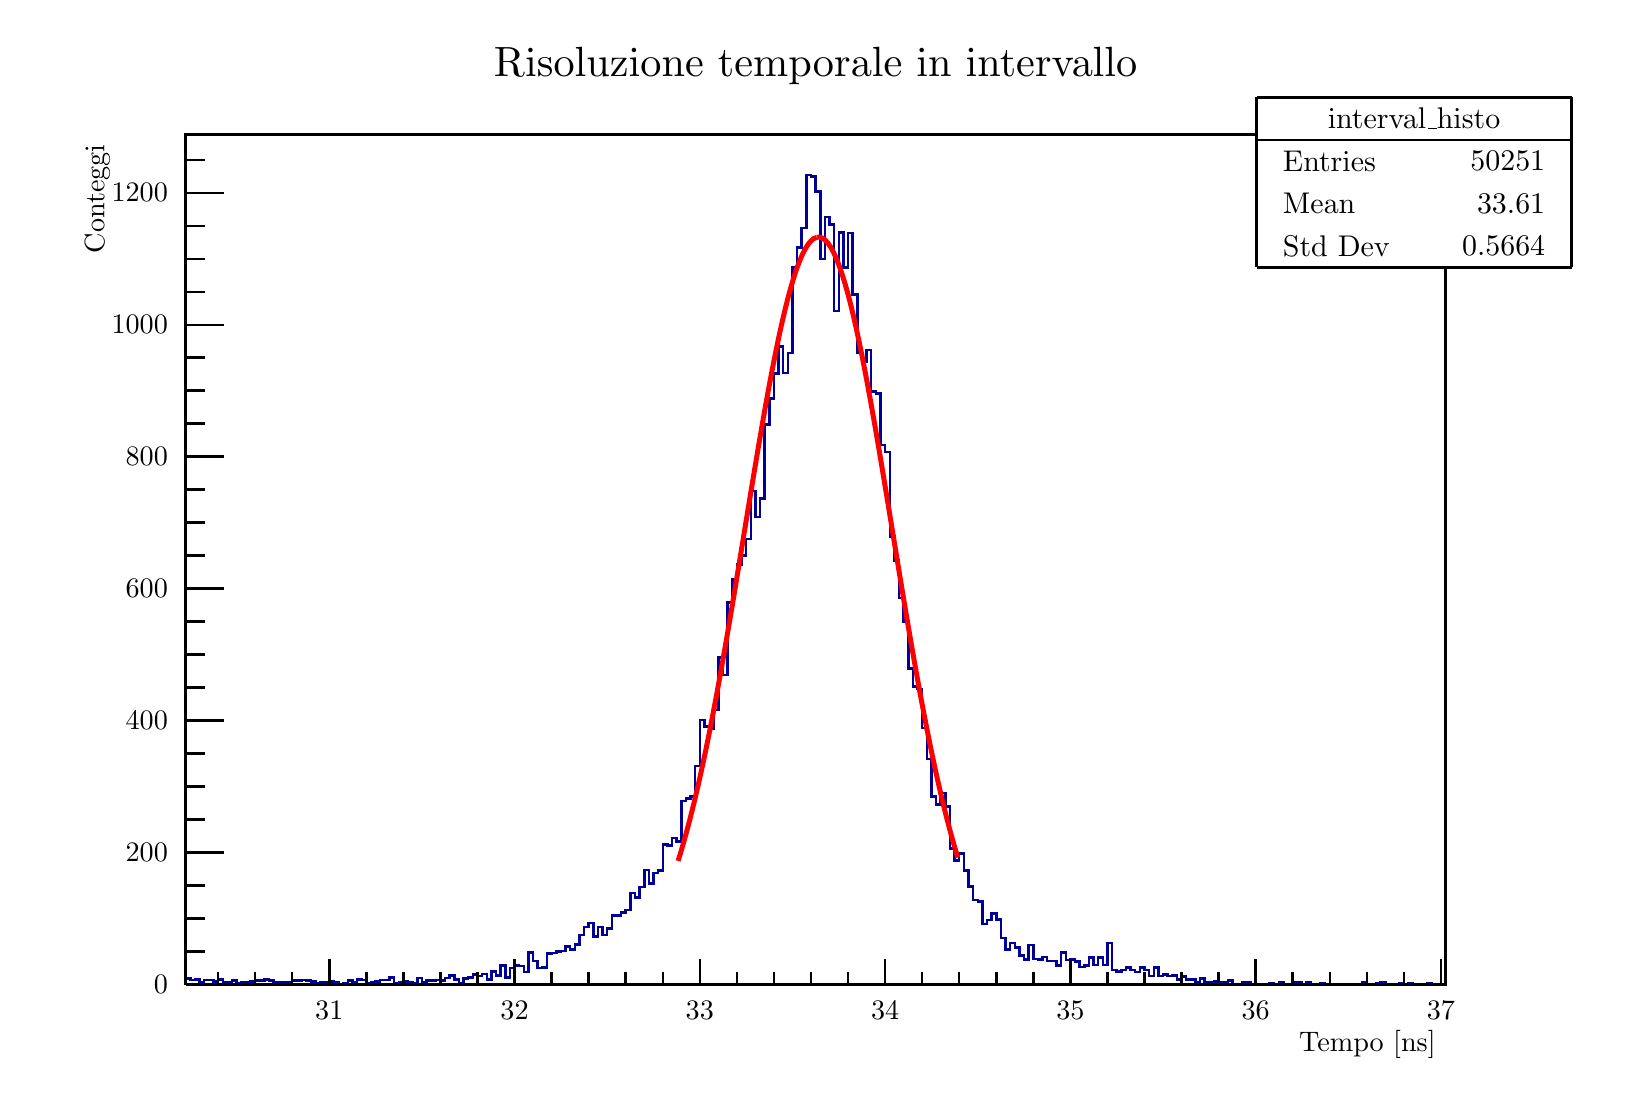
\begin{tikzpicture}
\pgfdeclareplotmark{cross} {
\pgfpathmoveto{\pgfpoint{-0.3\pgfplotmarksize}{\pgfplotmarksize}}
\pgfpathlineto{\pgfpoint{+0.3\pgfplotmarksize}{\pgfplotmarksize}}
\pgfpathlineto{\pgfpoint{+0.3\pgfplotmarksize}{0.3\pgfplotmarksize}}
\pgfpathlineto{\pgfpoint{+1\pgfplotmarksize}{0.3\pgfplotmarksize}}
\pgfpathlineto{\pgfpoint{+1\pgfplotmarksize}{-0.3\pgfplotmarksize}}
\pgfpathlineto{\pgfpoint{+0.3\pgfplotmarksize}{-0.3\pgfplotmarksize}}
\pgfpathlineto{\pgfpoint{+0.3\pgfplotmarksize}{-1.\pgfplotmarksize}}
\pgfpathlineto{\pgfpoint{-0.3\pgfplotmarksize}{-1.\pgfplotmarksize}}
\pgfpathlineto{\pgfpoint{-0.3\pgfplotmarksize}{-0.3\pgfplotmarksize}}
\pgfpathlineto{\pgfpoint{-1.\pgfplotmarksize}{-0.3\pgfplotmarksize}}
\pgfpathlineto{\pgfpoint{-1.\pgfplotmarksize}{0.3\pgfplotmarksize}}
\pgfpathlineto{\pgfpoint{-0.3\pgfplotmarksize}{0.3\pgfplotmarksize}}
\pgfpathclose
\pgfusepathqstroke
}
\pgfdeclareplotmark{cross*} {
\pgfpathmoveto{\pgfpoint{-0.3\pgfplotmarksize}{\pgfplotmarksize}}
\pgfpathlineto{\pgfpoint{+0.3\pgfplotmarksize}{\pgfplotmarksize}}
\pgfpathlineto{\pgfpoint{+0.3\pgfplotmarksize}{0.3\pgfplotmarksize}}
\pgfpathlineto{\pgfpoint{+1\pgfplotmarksize}{0.3\pgfplotmarksize}}
\pgfpathlineto{\pgfpoint{+1\pgfplotmarksize}{-0.3\pgfplotmarksize}}
\pgfpathlineto{\pgfpoint{+0.3\pgfplotmarksize}{-0.3\pgfplotmarksize}}
\pgfpathlineto{\pgfpoint{+0.3\pgfplotmarksize}{-1.\pgfplotmarksize}}
\pgfpathlineto{\pgfpoint{-0.3\pgfplotmarksize}{-1.\pgfplotmarksize}}
\pgfpathlineto{\pgfpoint{-0.3\pgfplotmarksize}{-0.3\pgfplotmarksize}}
\pgfpathlineto{\pgfpoint{-1.\pgfplotmarksize}{-0.3\pgfplotmarksize}}
\pgfpathlineto{\pgfpoint{-1.\pgfplotmarksize}{0.3\pgfplotmarksize}}
\pgfpathlineto{\pgfpoint{-0.3\pgfplotmarksize}{0.3\pgfplotmarksize}}
\pgfpathclose
\pgfusepathqfillstroke
}
\pgfdeclareplotmark{newstar} {
\pgfpathmoveto{\pgfqpoint{0pt}{\pgfplotmarksize}}
\pgfpathlineto{\pgfqpointpolar{44}{0.5\pgfplotmarksize}}
\pgfpathlineto{\pgfqpointpolar{18}{\pgfplotmarksize}}
\pgfpathlineto{\pgfqpointpolar{-20}{0.5\pgfplotmarksize}}
\pgfpathlineto{\pgfqpointpolar{-54}{\pgfplotmarksize}}
\pgfpathlineto{\pgfqpointpolar{-90}{0.5\pgfplotmarksize}}
\pgfpathlineto{\pgfqpointpolar{234}{\pgfplotmarksize}}
\pgfpathlineto{\pgfqpointpolar{198}{0.5\pgfplotmarksize}}
\pgfpathlineto{\pgfqpointpolar{162}{\pgfplotmarksize}}
\pgfpathlineto{\pgfqpointpolar{134}{0.5\pgfplotmarksize}}
\pgfpathclose
\pgfusepathqstroke
}
\pgfdeclareplotmark{newstar*} {
\pgfpathmoveto{\pgfqpoint{0pt}{\pgfplotmarksize}}
\pgfpathlineto{\pgfqpointpolar{44}{0.5\pgfplotmarksize}}
\pgfpathlineto{\pgfqpointpolar{18}{\pgfplotmarksize}}
\pgfpathlineto{\pgfqpointpolar{-20}{0.5\pgfplotmarksize}}
\pgfpathlineto{\pgfqpointpolar{-54}{\pgfplotmarksize}}
\pgfpathlineto{\pgfqpointpolar{-90}{0.5\pgfplotmarksize}}
\pgfpathlineto{\pgfqpointpolar{234}{\pgfplotmarksize}}
\pgfpathlineto{\pgfqpointpolar{198}{0.5\pgfplotmarksize}}
\pgfpathlineto{\pgfqpointpolar{162}{\pgfplotmarksize}}
\pgfpathlineto{\pgfqpointpolar{134}{0.5\pgfplotmarksize}}
\pgfpathclose
\pgfusepathqfillstroke
}
\definecolor{c}{rgb}{1,1,1};
\draw [color=c, fill=c] (0,0) rectangle (20,13.4957);
\draw [color=c, fill=c] (2,1.34957) rectangle (18,12.1461);
\definecolor{c}{rgb}{0,0,0};
\draw [c,line width=0.9] (2,1.34957) -- (2,12.1461) -- (18,12.1461) -- (18,1.34957) -- (2,1.34957);
\definecolor{c}{rgb}{1,1,1};
\draw [color=c, fill=c] (2,1.34957) rectangle (18,12.1461);
\definecolor{c}{rgb}{0,0,0};
\draw [c,line width=0.9] (2,1.34957) -- (2,12.1461) -- (18,12.1461) -- (18,1.34957) -- (2,1.34957);
\definecolor{c}{rgb}{0,0,0.6};
\draw [c,line width=0.9] (2,1.42499) -- (2.05882,1.42499) -- (2.05882,1.40823) -- (2.11765,1.40823) -- (2.11765,1.41661) -- (2.17647,1.41661) -- (2.17647,1.37471) -- (2.23529,1.37471) -- (2.23529,1.40823) -- (2.29412,1.40823) -- (2.29412,1.40823) --
 (2.35294,1.40823) -- (2.35294,1.39147) -- (2.41176,1.39147) -- (2.41176,1.41661) -- (2.47059,1.41661) -- (2.47059,1.38309) -- (2.52941,1.38309) -- (2.52941,1.37471) -- (2.58824,1.37471) -- (2.58824,1.39985) -- (2.64706,1.39985) -- (2.64706,1.36633)
 -- (2.70588,1.36633) -- (2.70588,1.38309) -- (2.76471,1.38309) -- (2.76471,1.38309) -- (2.82353,1.38309) -- (2.82353,1.39147) -- (2.88235,1.39147) -- (2.88235,1.39985) -- (2.94118,1.39985) -- (2.94118,1.39985) -- (3,1.39985) -- (3,1.41661) --
 (3.05882,1.41661) -- (3.05882,1.39985) -- (3.11765,1.39985) -- (3.11765,1.37471) -- (3.17647,1.37471) -- (3.17647,1.37471) -- (3.23529,1.37471) -- (3.23529,1.38309) -- (3.29412,1.38309) -- (3.29412,1.37471) -- (3.35294,1.37471) -- (3.35294,1.39985)
 -- (3.41176,1.39985) -- (3.41176,1.39985) -- (3.47059,1.39985) -- (3.47059,1.40823) -- (3.52941,1.40823) -- (3.52941,1.39985) -- (3.58824,1.39985) -- (3.58824,1.39147) -- (3.64706,1.39147) -- (3.64706,1.36633) -- (3.70588,1.36633) --
 (3.70588,1.38309) -- (3.76471,1.38309) -- (3.76471,1.38309) -- (3.82353,1.38309) -- (3.82353,1.39147) -- (3.88235,1.39147) -- (3.88235,1.37471) -- (3.94118,1.37471) -- (3.94118,1.35795) -- (4,1.35795) -- (4,1.36633) -- (4.05882,1.36633) --
 (4.05882,1.39985) -- (4.11765,1.39985) -- (4.11765,1.37471) -- (4.17647,1.37471) -- (4.17647,1.41661) -- (4.23529,1.41661) -- (4.23529,1.40823) -- (4.29412,1.40823) -- (4.29412,1.36633) -- (4.35294,1.36633) -- (4.35294,1.37471) -- (4.41176,1.37471)
 -- (4.41176,1.39147) -- (4.47059,1.39147) -- (4.47059,1.40823) -- (4.52941,1.40823) -- (4.52941,1.40823) -- (4.58824,1.40823) -- (4.58824,1.44175) -- (4.64706,1.44175) -- (4.64706,1.36633) -- (4.70588,1.36633) -- (4.70588,1.37471) --
 (4.76471,1.37471) -- (4.76471,1.39147) -- (4.82353,1.39147) -- (4.82353,1.37471) -- (4.88235,1.37471) -- (4.88235,1.36633) -- (4.94118,1.36633) -- (4.94118,1.43337) -- (5,1.43337) -- (5,1.37471) -- (5.05882,1.37471) -- (5.05882,1.39985) --
 (5.11765,1.39985) -- (5.11765,1.39985) -- (5.17647,1.39985) -- (5.17647,1.40823) -- (5.23529,1.40823) -- (5.23529,1.39985) -- (5.29412,1.39985) -- (5.29412,1.43337) -- (5.35294,1.43337) -- (5.35294,1.46689) -- (5.41176,1.46689) -- (5.41176,1.41661)
 -- (5.47059,1.41661) -- (5.47059,1.36633) -- (5.52941,1.36633) -- (5.52941,1.42499) -- (5.58824,1.42499) -- (5.58824,1.44175) -- (5.64706,1.44175) -- (5.64706,1.47527) -- (5.70588,1.47527) -- (5.70588,1.45851) -- (5.76471,1.45851) --
 (5.76471,1.48365) -- (5.82353,1.48365) -- (5.82353,1.41661) -- (5.88235,1.41661) -- (5.88235,1.51717) -- (5.94118,1.51717) -- (5.94118,1.46689) -- (6,1.46689) -- (6,1.59259) -- (6.05882,1.59259) -- (6.05882,1.44175) -- (6.11765,1.44175) --
 (6.11765,1.55907) -- (6.17647,1.55907) -- (6.17647,1.59259) -- (6.23529,1.59259) -- (6.23529,1.58421) -- (6.29412,1.58421) -- (6.29412,1.50879) -- (6.35294,1.50879) -- (6.35294,1.7602) -- (6.41176,1.7602) -- (6.41176,1.65126) -- (6.47059,1.65126) --
 (6.47059,1.55907) -- (6.52941,1.55907) -- (6.52941,1.56745) -- (6.58824,1.56745) -- (6.58824,1.74344) -- (6.64706,1.74344) -- (6.64706,1.75182) -- (6.70588,1.75182) -- (6.70588,1.76858) -- (6.76471,1.76858) -- (6.76471,1.77696) -- (6.82353,1.77696)
 -- (6.82353,1.83562) -- (6.88235,1.83562) -- (6.88235,1.79372) -- (6.94118,1.79372) -- (6.94118,1.86076) -- (7,1.86076) -- (7,1.97808) -- (7.05882,1.97808) -- (7.05882,2.07864) -- (7.11765,2.07864) -- (7.11765,2.12892) -- (7.17647,2.12892) --
 (7.17647,1.96132) -- (7.23529,1.96132) -- (7.23529,2.07864) -- (7.29412,2.07864) -- (7.29412,1.97808) -- (7.35294,1.97808) -- (7.35294,2.06188) -- (7.41176,2.06188) -- (7.41176,2.22949) -- (7.47059,2.22949) -- (7.47059,2.22949) -- (7.52941,2.22949)
 -- (7.52941,2.26301) -- (7.58824,2.26301) -- (7.58824,2.29653) -- (7.64706,2.29653) -- (7.64706,2.51441) -- (7.70588,2.51441) -- (7.70588,2.45575) -- (7.76471,2.45575) -- (7.76471,2.58983) -- (7.82353,2.58983) -- (7.82353,2.80772) --
 (7.88235,2.80772) -- (7.88235,2.63173) -- (7.94118,2.63173) -- (7.94118,2.76582) -- (8,2.76582) -- (8,2.79934) -- (8.05882,2.79934) -- (8.05882,3.12616) -- (8.11765,3.12616) -- (8.11765,3.11778) -- (8.17647,3.11778) -- (8.17647,3.20996) --
 (8.23529,3.20996) -- (8.23529,3.16806) -- (8.29412,3.16806) -- (8.29412,3.67925) -- (8.35294,3.67925) -- (8.35294,3.71277) -- (8.41177,3.71277) -- (8.41177,3.73791) -- (8.47059,3.73791) -- (8.47059,4.1234) -- (8.52941,4.1234) -- (8.52941,4.71001) --
 (8.58823,4.71001) -- (8.58823,4.62621) -- (8.64706,4.62621) -- (8.64706,4.60107) -- (8.70588,4.60107) -- (8.70588,4.83571) -- (8.76471,4.83571) -- (8.76471,5.50612) -- (8.82353,5.50612) -- (8.82353,5.27986) -- (8.88235,5.27986) -- (8.88235,6.20167)
 -- (8.94118,6.20167) -- (8.94118,6.50336) -- (9,6.50336) -- (9,6.68772) -- (9.05882,6.68772) -- (9.05882,6.79667) -- (9.11765,6.79667) -- (9.11765,7.00617) -- (9.17647,7.00617) -- (9.17647,7.61792) -- (9.23529,7.61792) -- (9.23529,7.29109) --
 (9.29412,7.29109) -- (9.29412,7.52574) -- (9.35294,7.52574) -- (9.35294,8.46431) -- (9.41177,8.46431) -- (9.41177,8.79114) -- (9.47059,8.79114) -- (9.47059,9.10959) -- (9.52941,9.10959) -- (9.52941,9.45317) -- (9.58823,9.45317) -- (9.58823,9.11797)
 -- (9.64706,9.11797) -- (9.64706,9.36937) -- (9.70588,9.36937) -- (9.70588,10.4588) -- (9.76471,10.4588) -- (9.76471,10.7102) -- (9.82353,10.7102) -- (9.82353,10.9616) -- (9.88235,10.9616) -- (9.88235,11.632) -- (9.94118,11.632) -- (9.94118,11.6152)
 -- (10,11.6152) -- (10,11.4225) -- (10.0588,11.4225) -- (10.0588,10.5677) -- (10.1176,10.5677) -- (10.1176,11.0957) -- (10.1765,11.0957) -- (10.1765,11.0035) -- (10.2353,11.0035) -- (10.2353,9.9057) -- (10.2941,9.9057) -- (10.2941,10.9029) --
 (10.3529,10.9029) -- (10.3529,10.4588) -- (10.4118,10.4588) -- (10.4118,10.8946) -- (10.4706,10.8946) -- (10.4706,10.1152) -- (10.5294,10.1152) -- (10.5294,9.36937) -- (10.5882,9.36937) -- (10.5882,9.26043) -- (10.6471,9.26043) -- (10.6471,9.41127)
 -- (10.7059,9.41127) -- (10.7059,8.88332) -- (10.7647,8.88332) -- (10.7647,8.85818) -- (10.8235,8.85818) -- (10.8235,8.20453) -- (10.8824,8.20453) -- (10.8824,8.11235) -- (10.9412,8.11235) -- (10.9412,7.03969) -- (11,7.03969) -- (11,6.738) --
 (11.0588,6.738) -- (11.0588,6.26034) -- (11.1176,6.26034) -- (11.1176,5.95865) -- (11.1765,5.95865) -- (11.1765,5.36366) -- (11.2353,5.36366) -- (11.2353,5.1374) -- (11.2941,5.1374) -- (11.2941,5.10388) -- (11.3529,5.10388) -- (11.3529,4.60945) --
 (11.4118,4.60945) -- (11.4118,4.21558) -- (11.4706,4.21558) -- (11.4706,3.73791) -- (11.5294,3.73791) -- (11.5294,3.63735) -- (11.5882,3.63735) -- (11.5882,3.77981) -- (11.6471,3.77981) -- (11.6471,3.61221) -- (11.7059,3.61221) -- (11.7059,3.07588)
 -- (11.7647,3.07588) -- (11.7647,2.92504) -- (11.8235,2.92504) -- (11.8235,3.01722) -- (11.8824,3.01722) -- (11.8824,2.79934) -- (11.9412,2.79934) -- (11.9412,2.59821) -- (12,2.59821) -- (12,2.42223) -- (12.0588,2.42223) -- (12.0588,2.40547) --
 (12.1176,2.40547) -- (12.1176,2.12054) -- (12.1765,2.12054) -- (12.1765,2.17082) -- (12.2353,2.17082) -- (12.2353,2.25463) -- (12.2941,2.25463) -- (12.2941,2.1792) -- (12.3529,2.1792) -- (12.3529,1.94456) -- (12.4118,1.94456) -- (12.4118,1.79372) --
 (12.4706,1.79372) -- (12.4706,1.87752) -- (12.5294,1.87752) -- (12.5294,1.81886) -- (12.5882,1.81886) -- (12.5882,1.7183) -- (12.6471,1.7183) -- (12.6471,1.66802) -- (12.7059,1.66802) -- (12.7059,1.85238) -- (12.7647,1.85238) -- (12.7647,1.6764) --
 (12.8235,1.6764) -- (12.8235,1.66802) -- (12.8824,1.66802) -- (12.8824,1.70154) -- (12.9412,1.70154) -- (12.9412,1.65126) -- (13,1.65126) -- (13,1.65126) -- (13.0588,1.65126) -- (13.0588,1.59259) -- (13.1176,1.59259) -- (13.1176,1.7602) --
 (13.1765,1.7602) -- (13.1765,1.65964) -- (13.2353,1.65964) -- (13.2353,1.66802) -- (13.2941,1.66802) -- (13.2941,1.64288) -- (13.3529,1.64288) -- (13.3529,1.57583) -- (13.4118,1.57583) -- (13.4118,1.59259) -- (13.4706,1.59259) -- (13.4706,1.69316)
 -- (13.5294,1.69316) -- (13.5294,1.60097) -- (13.5882,1.60097) -- (13.5882,1.69316) -- (13.6471,1.69316) -- (13.6471,1.60097) -- (13.7059,1.60097) -- (13.7059,1.87752) -- (13.7647,1.87752) -- (13.7647,1.53393) -- (13.8235,1.53393) --
 (13.8235,1.51717) -- (13.8824,1.51717) -- (13.8824,1.53393) -- (13.9412,1.53393) -- (13.9412,1.56745) -- (14,1.56745) -- (14,1.53393) -- (14.0588,1.53393) -- (14.0588,1.50879) -- (14.1176,1.50879) -- (14.1176,1.56745) -- (14.1765,1.56745) --
 (14.1765,1.53393) -- (14.2353,1.53393) -- (14.2353,1.45851) -- (14.2941,1.45851) -- (14.2941,1.56745) -- (14.3529,1.56745) -- (14.3529,1.45851) -- (14.4118,1.45851) -- (14.4118,1.47527) -- (14.4706,1.47527) -- (14.4706,1.45851) -- (14.5294,1.45851)
 -- (14.5294,1.46689) -- (14.5882,1.46689) -- (14.5882,1.41661) -- (14.6471,1.41661) -- (14.6471,1.45013) -- (14.7059,1.45013) -- (14.7059,1.41661) -- (14.7647,1.41661) -- (14.7647,1.41661) -- (14.8235,1.41661) -- (14.8235,1.38309) --
 (14.8824,1.38309) -- (14.8824,1.42499) -- (14.9412,1.42499) -- (14.9412,1.37471) -- (15,1.37471) -- (15,1.37471) -- (15.0588,1.37471) -- (15.0588,1.39147) -- (15.1176,1.39147) -- (15.1176,1.37471) -- (15.1765,1.37471) -- (15.1765,1.37471) --
 (15.2353,1.37471) -- (15.2353,1.39985) -- (15.2941,1.39985) -- (15.2941,1.35795) -- (15.3529,1.35795) -- (15.3529,1.34957) -- (15.4118,1.34957) -- (15.4118,1.38309) -- (15.4706,1.38309) -- (15.4706,1.37471) -- (15.5294,1.37471) -- (15.5294,1.35795)
 -- (15.5882,1.35795) -- (15.5882,1.35795) -- (15.6471,1.35795) -- (15.6471,1.34957) -- (15.7059,1.34957) -- (15.7059,1.35795) -- (15.7647,1.35795) -- (15.7647,1.36633) -- (15.8235,1.36633) -- (15.8235,1.35795) -- (15.8824,1.35795) --
 (15.8824,1.37471) -- (15.9412,1.37471) -- (15.9412,1.34957) -- (16,1.34957) -- (16,1.34957) -- (16.0588,1.34957) -- (16.0588,1.38309) -- (16.1176,1.38309) -- (16.1176,1.37471) -- (16.1765,1.37471) -- (16.1765,1.34957) -- (16.2353,1.34957) --
 (16.2353,1.37471) -- (16.2941,1.37471) -- (16.2941,1.35795) -- (16.3529,1.35795) -- (16.3529,1.35795) -- (16.4118,1.35795) -- (16.4118,1.36633) -- (16.4706,1.36633) -- (16.4706,1.35795) -- (16.5294,1.35795) -- (16.5294,1.34957) -- (16.5882,1.34957)
 -- (16.5882,1.35795) -- (16.6471,1.35795) -- (16.6471,1.35795) -- (16.7059,1.35795) -- (16.7059,1.34957) -- (16.7647,1.34957) -- (16.7647,1.35795) -- (16.8235,1.35795) -- (16.8235,1.34957) -- (16.8824,1.34957) -- (16.8824,1.34957) --
 (16.9412,1.34957) -- (16.9412,1.38309) -- (17,1.38309) -- (17,1.35795) -- (17.0588,1.35795) -- (17.0588,1.35795) -- (17.1176,1.35795) -- (17.1176,1.36633) -- (17.1765,1.36633) -- (17.1765,1.38309) -- (17.2353,1.38309) -- (17.2353,1.35795) --
 (17.2941,1.35795) -- (17.2941,1.34957) -- (17.3529,1.34957) -- (17.3529,1.35795) -- (17.4118,1.35795) -- (17.4118,1.36633) -- (17.4706,1.36633) -- (17.4706,1.34957) -- (17.5294,1.34957) -- (17.5294,1.36633) -- (17.5882,1.36633) -- (17.5882,1.35795)
 -- (17.6471,1.35795) -- (17.6471,1.35795) -- (17.7059,1.35795) -- (17.7059,1.35795) -- (17.7647,1.35795) -- (17.7647,1.36633) -- (17.8235,1.36633) -- (17.8235,1.34957) -- (17.8824,1.34957) -- (17.8824,1.35795) -- (17.9412,1.35795) --
 (17.9412,1.34957) -- (18,1.34957);
\definecolor{c}{rgb}{1,1,1};
\draw [color=c, fill=c] (15.6,10.4592) rectangle (19.6,12.6185);
\definecolor{c}{rgb}{0,0,0};
\draw [c,line width=0.9] (15.6,10.4592) -- (19.6,10.4592);
\draw [c,line width=0.9] (19.6,10.4592) -- (19.6,12.6185);
\draw [c,line width=0.9] (19.6,12.6185) -- (15.6,12.6185);
\draw [c,line width=0.9] (15.6,12.6185) -- (15.6,10.4592);
\draw (17.6,12.3486) node[scale=1.08185, color=c, rotate=0]{interval\_histo};
\draw [c,line width=0.9] (15.6,12.0787) -- (19.6,12.0787);
\draw [anchor= west] (15.8,11.8087) node[scale=1.08185, color=c, rotate=0]{Entries };
\draw [anchor= east] (19.4,11.8087) node[scale=1.08185, color=c, rotate=0]{ 50251};
\draw [anchor= west] (15.8,11.2689) node[scale=1.08185, color=c, rotate=0]{Mean  };
\draw [anchor= east] (19.4,11.2689) node[scale=1.08185, color=c, rotate=0]{  33.61};
\draw [anchor= west] (15.8,10.7291) node[scale=1.08185, color=c, rotate=0]{Std Dev   };
\draw [anchor= east] (19.4,10.7291) node[scale=1.08185, color=c, rotate=0]{ 0.5664};
\definecolor{c}{rgb}{1,0,0};
\draw [c,line width=1.8] (8.25323,2.92077) -- (8.28912,3.03752) -- (8.325,3.16031) -- (8.36088,3.2892) -- (8.39676,3.42424) -- (8.43265,3.56545) -- (8.46853,3.71283) -- (8.50441,3.86633) -- (8.54029,4.02591) -- (8.57618,4.19146) -- (8.61206,4.36285)
 -- (8.64794,4.53993) -- (8.68382,4.7225) -- (8.71971,4.91032) -- (8.75559,5.10313) -- (8.79147,5.30061) -- (8.82735,5.50243) -- (8.86324,5.7082) -- (8.89912,5.91751) -- (8.935,6.12989) -- (8.97088,6.34487) -- (9.00676,6.56191) -- (9.04265,6.78047)
 -- (9.07853,6.99994) -- (9.11441,7.21973) -- (9.15029,7.43919) -- (9.18618,7.65765) -- (9.22206,7.87443) -- (9.25794,8.08884) -- (9.29382,8.30016) -- (9.32971,8.50766) -- (9.36559,8.71062) -- (9.40147,8.90832) -- (9.43735,9.10002) --
 (9.47324,9.28501) -- (9.50912,9.46259) -- (9.545,9.63206) -- (9.58088,9.79276) -- (9.61677,9.94405) -- (9.65265,10.0853) -- (9.68853,10.216) -- (9.72441,10.3355) -- (9.76029,10.4433) -- (9.79618,10.539) -- (9.83206,10.6223) -- (9.86794,10.6926) --
 (9.90382,10.7498) -- (9.93971,10.7936) -- (9.97559,10.8237) -- (10.0115,10.8401);
\draw [c,line width=1.8] (10.0115,10.8401) -- (10.0474,10.8427) -- (10.0832,10.8315) -- (10.1191,10.8065) -- (10.155,10.7678) -- (10.1909,10.7156) -- (10.2268,10.6501) -- (10.2626,10.5717) -- (10.2985,10.4806) -- (10.3344,10.3772) -- (10.3703,10.262)
 -- (10.4062,10.1355) -- (10.4421,9.99813) -- (10.4779,9.85053) -- (10.5138,9.69328) -- (10.5497,9.52701) -- (10.5856,9.35239) -- (10.6215,9.17009) -- (10.6574,8.98081) -- (10.6932,8.78528) -- (10.7291,8.5842) -- (10.765,8.37831) -- (10.8009,8.16834)
 -- (10.8368,7.955) -- (10.8726,7.73903) -- (10.9085,7.52111) -- (10.9444,7.30195) -- (10.9803,7.08221) -- (11.0162,6.86254) -- (11.0521,6.64357) -- (11.0879,6.4259) -- (11.1238,6.21008) -- (11.1597,5.99667) -- (11.1956,5.78616) -- (11.2315,5.57901)
 -- (11.2674,5.37566) -- (11.3032,5.17652) -- (11.3391,4.98192) -- (11.375,4.7922) -- (11.4109,4.60764) -- (11.4468,4.42848) -- (11.4826,4.25494) -- (11.5185,4.08718) -- (11.5544,3.92536) -- (11.5903,3.76957) -- (11.6262,3.6199) -- (11.6621,3.47638)
 -- (11.6979,3.33903) -- (11.7338,3.20784) -- (11.7697,3.08277);
\draw [c,line width=1.8] (11.7697,3.08277) -- (11.8056,2.96377);
\definecolor{c}{rgb}{0,0,0};
\draw [c,line width=0.9] (2,1.34957) -- (18,1.34957);
\draw [anchor= east] (18,0.593811) node[scale=1.01821, color=c, rotate=0]{Tempo [ns]};
\draw [c,line width=0.9] (3.82353,1.67347) -- (3.82353,1.34957);
\draw [c,line width=0.9] (4.29412,1.51152) -- (4.29412,1.34957);
\draw [c,line width=0.9] (4.76471,1.51152) -- (4.76471,1.34957);
\draw [c,line width=0.9] (5.23529,1.51152) -- (5.23529,1.34957);
\draw [c,line width=0.9] (5.70588,1.51152) -- (5.70588,1.34957);
\draw [c,line width=0.9] (6.17647,1.67347) -- (6.17647,1.34957);
\draw [c,line width=0.9] (6.64706,1.51152) -- (6.64706,1.34957);
\draw [c,line width=0.9] (7.11765,1.51152) -- (7.11765,1.34957);
\draw [c,line width=0.9] (7.58824,1.51152) -- (7.58824,1.34957);
\draw [c,line width=0.9] (8.05882,1.51152) -- (8.05882,1.34957);
\draw [c,line width=0.9] (8.52941,1.67347) -- (8.52941,1.34957);
\draw [c,line width=0.9] (9,1.51152) -- (9,1.34957);
\draw [c,line width=0.9] (9.47059,1.51152) -- (9.47059,1.34957);
\draw [c,line width=0.9] (9.94118,1.51152) -- (9.94118,1.34957);
\draw [c,line width=0.9] (10.4118,1.51152) -- (10.4118,1.34957);
\draw [c,line width=0.9] (10.8824,1.67347) -- (10.8824,1.34957);
\draw [c,line width=0.9] (11.3529,1.51152) -- (11.3529,1.34957);
\draw [c,line width=0.9] (11.8235,1.51152) -- (11.8235,1.34957);
\draw [c,line width=0.9] (12.2941,1.51152) -- (12.2941,1.34957);
\draw [c,line width=0.9] (12.7647,1.51152) -- (12.7647,1.34957);
\draw [c,line width=0.9] (13.2353,1.67347) -- (13.2353,1.34957);
\draw [c,line width=0.9] (13.7059,1.51152) -- (13.7059,1.34957);
\draw [c,line width=0.9] (14.1765,1.51152) -- (14.1765,1.34957);
\draw [c,line width=0.9] (14.6471,1.51152) -- (14.6471,1.34957);
\draw [c,line width=0.9] (15.1176,1.51152) -- (15.1176,1.34957);
\draw [c,line width=0.9] (15.5882,1.67347) -- (15.5882,1.34957);
\draw [c,line width=0.9] (16.0588,1.51152) -- (16.0588,1.34957);
\draw [c,line width=0.9] (16.5294,1.51152) -- (16.5294,1.34957);
\draw [c,line width=0.9] (17,1.51152) -- (17,1.34957);
\draw [c,line width=0.9] (17.4706,1.51152) -- (17.4706,1.34957);
\draw [c,line width=0.9] (17.9412,1.67347) -- (17.9412,1.34957);
\draw [c,line width=0.9] (3.82353,1.67347) -- (3.82353,1.34957);
\draw [c,line width=0.9] (3.35294,1.51152) -- (3.35294,1.34957);
\draw [c,line width=0.9] (2.88235,1.51152) -- (2.88235,1.34957);
\draw [c,line width=0.9] (2.41176,1.51152) -- (2.41176,1.34957);
\draw [c,line width=0.9] (17.9412,1.67347) -- (17.9412,1.34957);
\draw [anchor=base] (3.82353,0.904212) node[scale=1.01821, color=c, rotate=0]{31};
\draw [anchor=base] (6.17647,0.904212) node[scale=1.01821, color=c, rotate=0]{32};
\draw [anchor=base] (8.52941,0.904212) node[scale=1.01821, color=c, rotate=0]{33};
\draw [anchor=base] (10.8824,0.904212) node[scale=1.01821, color=c, rotate=0]{34};
\draw [anchor=base] (13.2353,0.904212) node[scale=1.01821, color=c, rotate=0]{35};
\draw [anchor=base] (15.5882,0.904212) node[scale=1.01821, color=c, rotate=0]{36};
\draw [anchor=base] (17.9412,0.904212) node[scale=1.01821, color=c, rotate=0]{37};
\draw [c,line width=0.9] (2,1.34957) -- (2,12.1461);
\draw [anchor= east] (0.88,12.1461) node[scale=1.01821, color=c, rotate=90]{Conteggi};
\draw [c,line width=0.9] (2.48,1.34957) -- (2,1.34957);
\draw [c,line width=0.9] (2.24,1.76858) -- (2,1.76858);
\draw [c,line width=0.9] (2.24,2.18758) -- (2,2.18758);
\draw [c,line width=0.9] (2.24,2.60659) -- (2,2.60659);
\draw [c,line width=0.9] (2.48,3.0256) -- (2,3.0256);
\draw [c,line width=0.9] (2.24,3.44461) -- (2,3.44461);
\draw [c,line width=0.9] (2.24,3.86361) -- (2,3.86361);
\draw [c,line width=0.9] (2.24,4.28262) -- (2,4.28262);
\draw [c,line width=0.9] (2.48,4.70163) -- (2,4.70163);
\draw [c,line width=0.9] (2.24,5.12064) -- (2,5.12064);
\draw [c,line width=0.9] (2.24,5.53964) -- (2,5.53964);
\draw [c,line width=0.9] (2.24,5.95865) -- (2,5.95865);
\draw [c,line width=0.9] (2.48,6.37766) -- (2,6.37766);
\draw [c,line width=0.9] (2.24,6.79667) -- (2,6.79667);
\draw [c,line width=0.9] (2.24,7.21567) -- (2,7.21567);
\draw [c,line width=0.9] (2.24,7.63468) -- (2,7.63468);
\draw [c,line width=0.9] (2.48,8.05369) -- (2,8.05369);
\draw [c,line width=0.9] (2.24,8.47269) -- (2,8.47269);
\draw [c,line width=0.9] (2.24,8.8917) -- (2,8.8917);
\draw [c,line width=0.9] (2.24,9.31071) -- (2,9.31071);
\draw [c,line width=0.9] (2.48,9.72972) -- (2,9.72972);
\draw [c,line width=0.9] (2.24,10.1487) -- (2,10.1487);
\draw [c,line width=0.9] (2.24,10.5677) -- (2,10.5677);
\draw [c,line width=0.9] (2.24,10.9867) -- (2,10.9867);
\draw [c,line width=0.9] (2.48,11.4057) -- (2,11.4057);
\draw [c,line width=0.9] (2.48,11.4057) -- (2,11.4057);
\draw [c,line width=0.9] (2.24,11.8248) -- (2,11.8248);
\draw [anchor= east] (1.9,1.34957) node[scale=1.01821, color=c, rotate=0]{0};
\draw [anchor= east] (1.9,3.0256) node[scale=1.01821, color=c, rotate=0]{200};
\draw [anchor= east] (1.9,4.70163) node[scale=1.01821, color=c, rotate=0]{400};
\draw [anchor= east] (1.9,6.37766) node[scale=1.01821, color=c, rotate=0]{600};
\draw [anchor= east] (1.9,8.05369) node[scale=1.01821, color=c, rotate=0]{800};
\draw [anchor= east] (1.9,9.72972) node[scale=1.01821, color=c, rotate=0]{1000};
\draw [anchor= east] (1.9,11.4057) node[scale=1.01821, color=c, rotate=0]{1200};
\definecolor{c}{rgb}{1,1,1};
\draw [color=c, fill=c] (15.6,10.4592) rectangle (19.6,12.6185);
\definecolor{c}{rgb}{0,0,0};
\draw [c,line width=0.9] (15.6,10.4592) -- (19.6,10.4592);
\draw [c,line width=0.9] (19.6,10.4592) -- (19.6,12.6185);
\draw [c,line width=0.9] (19.6,12.6185) -- (15.6,12.6185);
\draw [c,line width=0.9] (15.6,12.6185) -- (15.6,10.4592);
\draw (17.6,12.3486) node[scale=1.08185, color=c, rotate=0]{interval\_histo};
\draw [c,line width=0.9] (15.6,12.0787) -- (19.6,12.0787);
\draw [anchor= west] (15.8,11.8087) node[scale=1.08185, color=c, rotate=0]{Entries };
\draw [anchor= east] (19.4,11.8087) node[scale=1.08185, color=c, rotate=0]{ 50251};
\draw [anchor= west] (15.8,11.2689) node[scale=1.08185, color=c, rotate=0]{Mean  };
\draw [anchor= east] (19.4,11.2689) node[scale=1.08185, color=c, rotate=0]{  33.61};
\draw [anchor= west] (15.8,10.7291) node[scale=1.08185, color=c, rotate=0]{Std Dev   };
\draw [anchor= east] (19.4,10.7291) node[scale=1.08185, color=c, rotate=0]{ 0.5664};
\draw (10,13.0156) node[scale=1.52731, color=c, rotate=0]{Risoluzione temporale in intervallo};
\end{tikzpicture}

%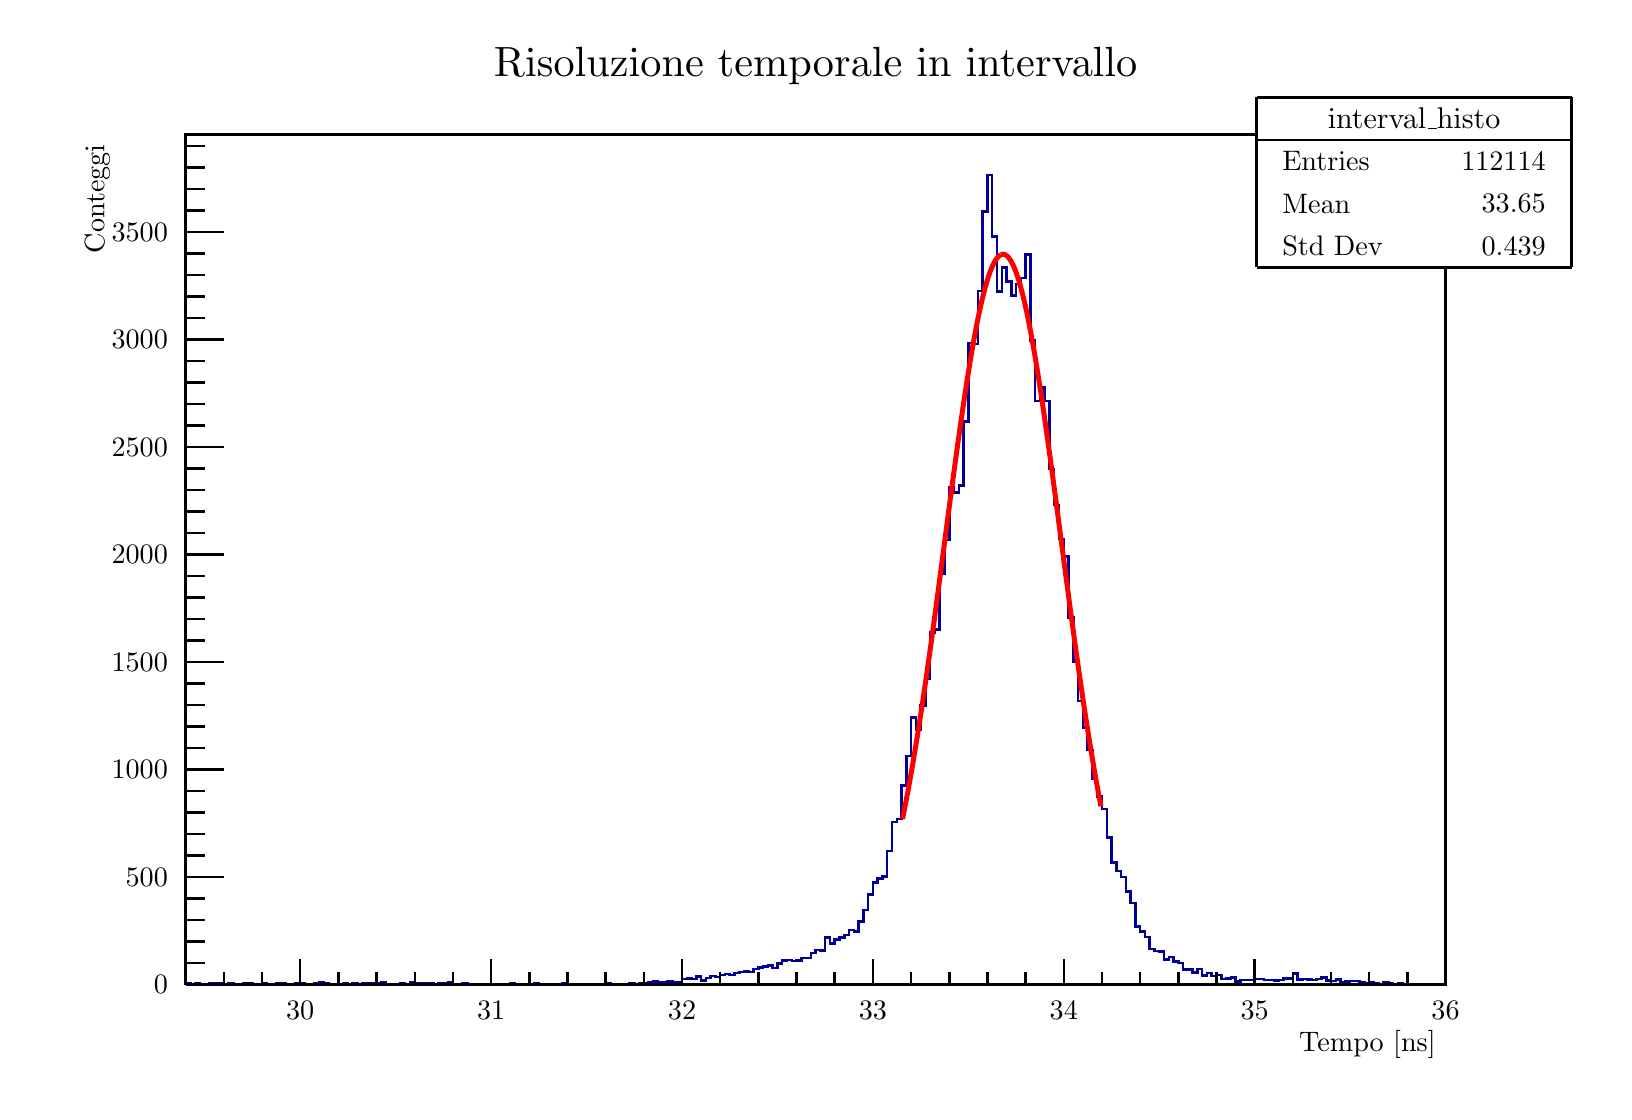
\begin{tikzpicture}
\pgfdeclareplotmark{cross} {
\pgfpathmoveto{\pgfpoint{-0.3\pgfplotmarksize}{\pgfplotmarksize}}
\pgfpathlineto{\pgfpoint{+0.3\pgfplotmarksize}{\pgfplotmarksize}}
\pgfpathlineto{\pgfpoint{+0.3\pgfplotmarksize}{0.3\pgfplotmarksize}}
\pgfpathlineto{\pgfpoint{+1\pgfplotmarksize}{0.3\pgfplotmarksize}}
\pgfpathlineto{\pgfpoint{+1\pgfplotmarksize}{-0.3\pgfplotmarksize}}
\pgfpathlineto{\pgfpoint{+0.3\pgfplotmarksize}{-0.3\pgfplotmarksize}}
\pgfpathlineto{\pgfpoint{+0.3\pgfplotmarksize}{-1.\pgfplotmarksize}}
\pgfpathlineto{\pgfpoint{-0.3\pgfplotmarksize}{-1.\pgfplotmarksize}}
\pgfpathlineto{\pgfpoint{-0.3\pgfplotmarksize}{-0.3\pgfplotmarksize}}
\pgfpathlineto{\pgfpoint{-1.\pgfplotmarksize}{-0.3\pgfplotmarksize}}
\pgfpathlineto{\pgfpoint{-1.\pgfplotmarksize}{0.3\pgfplotmarksize}}
\pgfpathlineto{\pgfpoint{-0.3\pgfplotmarksize}{0.3\pgfplotmarksize}}
\pgfpathclose
\pgfusepathqstroke
}
\pgfdeclareplotmark{cross*} {
\pgfpathmoveto{\pgfpoint{-0.3\pgfplotmarksize}{\pgfplotmarksize}}
\pgfpathlineto{\pgfpoint{+0.3\pgfplotmarksize}{\pgfplotmarksize}}
\pgfpathlineto{\pgfpoint{+0.3\pgfplotmarksize}{0.3\pgfplotmarksize}}
\pgfpathlineto{\pgfpoint{+1\pgfplotmarksize}{0.3\pgfplotmarksize}}
\pgfpathlineto{\pgfpoint{+1\pgfplotmarksize}{-0.3\pgfplotmarksize}}
\pgfpathlineto{\pgfpoint{+0.3\pgfplotmarksize}{-0.3\pgfplotmarksize}}
\pgfpathlineto{\pgfpoint{+0.3\pgfplotmarksize}{-1.\pgfplotmarksize}}
\pgfpathlineto{\pgfpoint{-0.3\pgfplotmarksize}{-1.\pgfplotmarksize}}
\pgfpathlineto{\pgfpoint{-0.3\pgfplotmarksize}{-0.3\pgfplotmarksize}}
\pgfpathlineto{\pgfpoint{-1.\pgfplotmarksize}{-0.3\pgfplotmarksize}}
\pgfpathlineto{\pgfpoint{-1.\pgfplotmarksize}{0.3\pgfplotmarksize}}
\pgfpathlineto{\pgfpoint{-0.3\pgfplotmarksize}{0.3\pgfplotmarksize}}
\pgfpathclose
\pgfusepathqfillstroke
}
\pgfdeclareplotmark{newstar} {
\pgfpathmoveto{\pgfqpoint{0pt}{\pgfplotmarksize}}
\pgfpathlineto{\pgfqpointpolar{44}{0.5\pgfplotmarksize}}
\pgfpathlineto{\pgfqpointpolar{18}{\pgfplotmarksize}}
\pgfpathlineto{\pgfqpointpolar{-20}{0.5\pgfplotmarksize}}
\pgfpathlineto{\pgfqpointpolar{-54}{\pgfplotmarksize}}
\pgfpathlineto{\pgfqpointpolar{-90}{0.5\pgfplotmarksize}}
\pgfpathlineto{\pgfqpointpolar{234}{\pgfplotmarksize}}
\pgfpathlineto{\pgfqpointpolar{198}{0.5\pgfplotmarksize}}
\pgfpathlineto{\pgfqpointpolar{162}{\pgfplotmarksize}}
\pgfpathlineto{\pgfqpointpolar{134}{0.5\pgfplotmarksize}}
\pgfpathclose
\pgfusepathqstroke
}
\pgfdeclareplotmark{newstar*} {
\pgfpathmoveto{\pgfqpoint{0pt}{\pgfplotmarksize}}
\pgfpathlineto{\pgfqpointpolar{44}{0.5\pgfplotmarksize}}
\pgfpathlineto{\pgfqpointpolar{18}{\pgfplotmarksize}}
\pgfpathlineto{\pgfqpointpolar{-20}{0.5\pgfplotmarksize}}
\pgfpathlineto{\pgfqpointpolar{-54}{\pgfplotmarksize}}
\pgfpathlineto{\pgfqpointpolar{-90}{0.5\pgfplotmarksize}}
\pgfpathlineto{\pgfqpointpolar{234}{\pgfplotmarksize}}
\pgfpathlineto{\pgfqpointpolar{198}{0.5\pgfplotmarksize}}
\pgfpathlineto{\pgfqpointpolar{162}{\pgfplotmarksize}}
\pgfpathlineto{\pgfqpointpolar{134}{0.5\pgfplotmarksize}}
\pgfpathclose
\pgfusepathqfillstroke
}
\definecolor{c}{rgb}{1,1,1};
\draw [color=c, fill=c] (0,0) rectangle (20,13.4957);
\draw [color=c, fill=c] (2,1.34957) rectangle (18,12.1461);
\definecolor{c}{rgb}{0,0,0};
\draw [c,line width=0.9] (2,1.34957) -- (2,12.1461) -- (18,12.1461) -- (18,1.34957) -- (2,1.34957);
\definecolor{c}{rgb}{1,1,1};
\draw [color=c, fill=c] (2,1.34957) rectangle (18,12.1461);
\definecolor{c}{rgb}{0,0,0};
\draw [c,line width=0.9] (2,1.34957) -- (2,12.1461) -- (18,12.1461) -- (18,1.34957) -- (2,1.34957);
\definecolor{c}{rgb}{0,0,0.6};
\draw [c,line width=0.9] (2,1.36323) -- (2.06061,1.36323) -- (2.06061,1.35776) -- (2.12121,1.35776) -- (2.12121,1.36323) -- (2.18182,1.36323) -- (2.18182,1.36049) -- (2.24242,1.36049) -- (2.24242,1.35503) -- (2.30303,1.35503) -- (2.30303,1.36323) --
 (2.36364,1.36323) -- (2.36364,1.36323) -- (2.42424,1.36323) -- (2.42424,1.36596) -- (2.48485,1.36596) -- (2.48485,1.36049) -- (2.54545,1.36049) -- (2.54545,1.36323) -- (2.60606,1.36323) -- (2.60606,1.36049) -- (2.66667,1.36049) -- (2.66667,1.36049)
 -- (2.72727,1.36049) -- (2.72727,1.36869) -- (2.78788,1.36869) -- (2.78788,1.37142) -- (2.84848,1.37142) -- (2.84848,1.35776) -- (2.90909,1.35776) -- (2.90909,1.35503) -- (2.9697,1.35503) -- (2.9697,1.36323) -- (3.0303,1.36323) -- (3.0303,1.35776)
 -- (3.09091,1.35776) -- (3.09091,1.35776) -- (3.15152,1.35776) -- (3.15152,1.36323) -- (3.21212,1.36323) -- (3.21212,1.36323) -- (3.27273,1.36323) -- (3.27273,1.36049) -- (3.33333,1.36049) -- (3.33333,1.35776) -- (3.39394,1.35776) --
 (3.39394,1.37142) -- (3.45455,1.37142) -- (3.45455,1.36323) -- (3.51515,1.36323) -- (3.51515,1.36049) -- (3.57576,1.36049) -- (3.57576,1.3523) -- (3.63636,1.3523) -- (3.63636,1.36596) -- (3.69697,1.36596) -- (3.69697,1.37688) -- (3.75758,1.37688) --
 (3.75758,1.36596) -- (3.81818,1.36596) -- (3.81818,1.35503) -- (3.87879,1.35503) -- (3.87879,1.36049) -- (3.93939,1.36049) -- (3.93939,1.36049) -- (4,1.36049) -- (4,1.36323) -- (4.06061,1.36323) -- (4.06061,1.35776) -- (4.12121,1.35776) --
 (4.12121,1.37142) -- (4.18182,1.37142) -- (4.18182,1.36049) -- (4.24242,1.36049) -- (4.24242,1.36323) -- (4.30303,1.36323) -- (4.30303,1.36596) -- (4.36364,1.36596) -- (4.36364,1.37142) -- (4.42424,1.37142) -- (4.42424,1.37142) -- (4.48485,1.37142)
 -- (4.48485,1.37688) -- (4.54545,1.37688) -- (4.54545,1.36049) -- (4.60606,1.36049) -- (4.60606,1.36049) -- (4.66667,1.36049) -- (4.66667,1.35503) -- (4.72727,1.35503) -- (4.72727,1.36596) -- (4.78788,1.36596) -- (4.78788,1.36049) --
 (4.84848,1.36049) -- (4.84848,1.37688) -- (4.90909,1.37688) -- (4.90909,1.36596) -- (4.9697,1.36596) -- (4.9697,1.36596) -- (5.0303,1.36596) -- (5.0303,1.36596) -- (5.09091,1.36596) -- (5.09091,1.36323) -- (5.15152,1.36323) -- (5.15152,1.35776) --
 (5.21212,1.35776) -- (5.21212,1.36596) -- (5.27273,1.36596) -- (5.27273,1.36323) -- (5.33333,1.36323) -- (5.33333,1.37961) -- (5.39394,1.37961) -- (5.39394,1.36049) -- (5.45455,1.36049) -- (5.45455,1.35776) -- (5.51515,1.35776) -- (5.51515,1.36596)
 -- (5.57576,1.36596) -- (5.57576,1.35776) -- (5.63636,1.35776) -- (5.63636,1.35776) -- (5.69697,1.35776) -- (5.69697,1.35776) -- (5.75758,1.35776) -- (5.75758,1.36049) -- (5.81818,1.36049) -- (5.81818,1.3523) -- (5.87879,1.3523) -- (5.87879,1.36049)
 -- (5.93939,1.36049) -- (5.93939,1.35776) -- (6,1.35776) -- (6,1.35776) -- (6.06061,1.35776) -- (6.06061,1.3523) -- (6.12121,1.3523) -- (6.12121,1.36869) -- (6.18182,1.36869) -- (6.18182,1.36049) -- (6.24242,1.36049) -- (6.24242,1.35776) --
 (6.30303,1.35776) -- (6.30303,1.36049) -- (6.36364,1.36049) -- (6.36364,1.3523) -- (6.42424,1.3523) -- (6.42424,1.36596) -- (6.48485,1.36596) -- (6.48485,1.35776) -- (6.54545,1.35776) -- (6.54545,1.35776) -- (6.60606,1.35776) -- (6.60606,1.3523) --
 (6.66667,1.3523) -- (6.66667,1.35503) -- (6.72727,1.35503) -- (6.72727,1.35776) -- (6.78788,1.35776) -- (6.78788,1.36323) -- (6.84848,1.36323) -- (6.84848,1.35776) -- (6.90909,1.35776) -- (6.90909,1.35503) -- (6.9697,1.35503) -- (6.9697,1.36049) --
 (7.0303,1.36049) -- (7.0303,1.35503) -- (7.09091,1.35503) -- (7.09091,1.35503) -- (7.15152,1.35503) -- (7.15152,1.3523) -- (7.21212,1.3523) -- (7.21212,1.35503) -- (7.27273,1.35503) -- (7.27273,1.35776) -- (7.33333,1.35776) -- (7.33333,1.36596) --
 (7.39394,1.36596) -- (7.39394,1.35503) -- (7.45455,1.35503) -- (7.45455,1.35776) -- (7.51515,1.35776) -- (7.51515,1.3523) -- (7.57576,1.3523) -- (7.57576,1.36049) -- (7.63636,1.36049) -- (7.63636,1.36323) -- (7.69697,1.36323) -- (7.69697,1.36049) --
 (7.75758,1.36049) -- (7.75758,1.36869) -- (7.81818,1.36869) -- (7.81818,1.36869) -- (7.87879,1.36869) -- (7.87879,1.37961) -- (7.93939,1.37961) -- (7.93939,1.38781) -- (8,1.38781) -- (8,1.37415) -- (8.06061,1.37415) -- (8.06061,1.37688) --
 (8.12121,1.37688) -- (8.12121,1.39054) -- (8.18182,1.39054) -- (8.18182,1.37961) -- (8.24242,1.37961) -- (8.24242,1.38507) -- (8.30303,1.38507) -- (8.30303,1.42058) -- (8.36364,1.42058) -- (8.36364,1.42604) -- (8.42424,1.42604) -- (8.42424,1.42058)
 -- (8.48485,1.42058) -- (8.48485,1.45062) -- (8.54545,1.45062) -- (8.54545,1.40419) -- (8.60606,1.40419) -- (8.60606,1.4315) -- (8.66667,1.4315) -- (8.66667,1.45608) -- (8.72727,1.45608) -- (8.72727,1.44789) -- (8.78788,1.44789) -- (8.78788,1.47247)
 -- (8.84848,1.47247) -- (8.84848,1.48339) -- (8.90909,1.48339) -- (8.90909,1.46974) -- (8.9697,1.46974) -- (8.9697,1.49432) -- (9.0303,1.49432) -- (9.0303,1.50797) -- (9.09091,1.50797) -- (9.09091,1.5189) -- (9.15152,1.5189) -- (9.15152,1.50797) --
 (9.21212,1.50797) -- (9.21212,1.54621) -- (9.27273,1.54621) -- (9.27273,1.56532) -- (9.33333,1.56532) -- (9.33333,1.57898) -- (9.39394,1.57898) -- (9.39394,1.59263) -- (9.45455,1.59263) -- (9.45455,1.56259) -- (9.51515,1.56259) -- (9.51515,1.61995)
 -- (9.57576,1.61995) -- (9.57576,1.65272) -- (9.63636,1.65272) -- (9.63636,1.66091) -- (9.69697,1.66091) -- (9.69697,1.64726) -- (9.75758,1.64726) -- (9.75758,1.65818) -- (9.81818,1.65818) -- (9.81818,1.68822) -- (9.87879,1.68822) --
 (9.87879,1.68822) -- (9.93939,1.68822) -- (9.93939,1.7483) -- (10,1.7483) -- (10,1.78927) -- (10.0606,1.78927) -- (10.0606,1.78108) -- (10.1212,1.78108) -- (10.1212,1.94767) -- (10.1818,1.94767) -- (10.1818,1.87393) -- (10.2424,1.87393) --
 (10.2424,1.92309) -- (10.303,1.92309) -- (10.303,1.94767) -- (10.3636,1.94767) -- (10.3636,1.98045) -- (10.4242,1.98045) -- (10.4242,2.04326) -- (10.4848,2.04326) -- (10.4848,2.02414) -- (10.5455,2.02414) -- (10.5455,2.1525) -- (10.6061,2.1525) --
 (10.6061,2.29725) -- (10.6667,2.29725) -- (10.6667,2.49662) -- (10.7273,2.49662) -- (10.7273,2.64682) -- (10.7879,2.64682) -- (10.7879,2.69871) -- (10.8485,2.69871) -- (10.8485,2.72329) -- (10.9091,2.72329) -- (10.9091,3.04829) -- (10.9697,3.04829)
 -- (10.9697,3.41425) -- (11.0303,3.41425) -- (11.0303,3.44976) -- (11.0909,3.44976) -- (11.0909,3.88126) -- (11.1515,3.88126) -- (11.1515,4.25542) -- (11.2121,4.25542) -- (11.2121,4.74155) -- (11.2727,4.74155) -- (11.2727,4.58861) --
 (11.3333,4.58861) -- (11.3333,4.89722) -- (11.3939,4.89722) -- (11.3939,5.23314) -- (11.4545,5.23314) -- (11.4545,5.82031) -- (11.5152,5.82031) -- (11.5152,5.85855) -- (11.5758,5.85855) -- (11.5758,6.56589) -- (11.6364,6.56589) -- (11.6364,6.99467)
 -- (11.697,6.99467) -- (11.697,7.66105) -- (11.7576,7.66105) -- (11.7576,7.60097) -- (11.8182,7.60097) -- (11.8182,7.68836) -- (11.8788,7.68836) -- (11.8788,8.49948) -- (11.9394,8.49948) -- (11.9394,9.49632) -- (12,9.49632) -- (12,9.48267) --
 (12.0606,9.48267) -- (12.0606,10.1572) -- (12.1212,10.1572) -- (12.1212,11.1677) -- (12.1818,11.1677) -- (12.1818,11.632) -- (12.2424,11.632) -- (12.2424,10.8509) -- (12.303,10.8509) -- (12.303,10.1545) -- (12.3636,10.1545) -- (12.3636,10.4549) --
 (12.4242,10.4549) -- (12.4242,10.2774) -- (12.4848,10.2774) -- (12.4848,10.0999) -- (12.5455,10.0999) -- (12.5455,10.2474) -- (12.6061,10.2474) -- (12.6061,10.3266) -- (12.6667,10.3266) -- (12.6667,10.6242) -- (12.7273,10.6242) -- (12.7273,9.53183)
 -- (12.7879,9.53183) -- (12.7879,8.75893) -- (12.8485,8.75893) -- (12.8485,8.93099) -- (12.9091,8.93099) -- (12.9091,8.75893) -- (12.9697,8.75893) -- (12.9697,7.89592) -- (13.0303,7.89592) -- (13.0303,7.44256) -- (13.0909,7.44256) --
 (13.0909,7.01106) -- (13.1515,7.01106) -- (13.1515,6.78711) -- (13.2121,6.78711) -- (13.2121,6.01422) -- (13.2727,6.01422) -- (13.2727,5.44889) -- (13.3333,5.44889) -- (13.3333,4.95457) -- (13.3939,4.95457) -- (13.3939,4.61592) -- (13.4545,4.61592)
 -- (13.4545,4.32916) -- (13.5152,4.32916) -- (13.5152,3.96319) -- (13.5758,3.96319) -- (13.5758,3.73925) -- (13.6364,3.73925) -- (13.6364,3.57811) -- (13.697,3.57811) -- (13.697,3.21762) -- (13.7576,3.21762) -- (13.7576,2.89808) -- (13.8182,2.89808)
 -- (13.8182,2.79157) -- (13.8788,2.79157) -- (13.8788,2.7151) -- (13.9394,2.7151) -- (13.9394,2.53485) -- (14,2.53485) -- (14,2.38737) -- (14.0606,2.38737) -- (14.0606,2.08696) -- (14.1212,2.08696) -- (14.1212,2.02687) -- (14.1818,2.02687) --
 (14.1818,1.95313) -- (14.2424,1.95313) -- (14.2424,1.8002) -- (14.303,1.8002) -- (14.303,1.77835) -- (14.3636,1.77835) -- (14.3636,1.77015) -- (14.4242,1.77015) -- (14.4242,1.6691) -- (14.4848,1.6691) -- (14.4848,1.70188) -- (14.5455,1.70188) --
 (14.5455,1.64179) -- (14.6061,1.64179) -- (14.6061,1.62541) -- (14.6667,1.62541) -- (14.6667,1.54074) -- (14.7273,1.54074) -- (14.7273,1.54348) -- (14.7879,1.54348) -- (14.7879,1.50524) -- (14.8485,1.50524) -- (14.8485,1.54621) -- (14.9091,1.54621)
 -- (14.9091,1.46427) -- (14.9697,1.46427) -- (14.9697,1.49978) -- (15.0303,1.49978) -- (15.0303,1.46154) -- (15.0909,1.46154) -- (15.0909,1.47247) -- (15.1515,1.47247) -- (15.1515,1.42058) -- (15.2121,1.42058) -- (15.2121,1.42877) --
 (15.2727,1.42877) -- (15.2727,1.4397) -- (15.3333,1.4397) -- (15.3333,1.39054) -- (15.3939,1.39054) -- (15.3939,1.40692) -- (15.4545,1.40692) -- (15.4545,1.40965) -- (15.5152,1.40965) -- (15.5152,1.40965) -- (15.5758,1.40965) -- (15.5758,1.41785) --
 (15.6364,1.41785) -- (15.6364,1.42331) -- (15.697,1.42331) -- (15.697,1.40692) -- (15.7576,1.40692) -- (15.7576,1.40965) -- (15.8182,1.40965) -- (15.8182,1.39873) -- (15.8788,1.39873) -- (15.8788,1.40692) -- (15.9394,1.40692) -- (15.9394,1.42877) --
 (16,1.42877) -- (16,1.42604) -- (16.0606,1.42604) -- (16.0606,1.49159) -- (16.1212,1.49159) -- (16.1212,1.41238) -- (16.1818,1.41238) -- (16.1818,1.42058) -- (16.2424,1.42058) -- (16.2424,1.41512) -- (16.303,1.41512) -- (16.303,1.40692) --
 (16.3636,1.40692) -- (16.3636,1.41785) -- (16.4242,1.41785) -- (16.4242,1.43696) -- (16.4848,1.43696) -- (16.4848,1.40146) -- (16.5455,1.40146) -- (16.5455,1.39327) -- (16.6061,1.39327) -- (16.6061,1.41238) -- (16.6667,1.41238) -- (16.6667,1.38507)
 -- (16.7273,1.38507) -- (16.7273,1.38781) -- (16.7879,1.38781) -- (16.7879,1.39327) -- (16.8485,1.39327) -- (16.8485,1.39327) -- (16.9091,1.39327) -- (16.9091,1.37961) -- (16.9697,1.37961) -- (16.9697,1.36323) -- (17.0303,1.36323) --
 (17.0303,1.37961) -- (17.0909,1.37961) -- (17.0909,1.37142) -- (17.1515,1.37142) -- (17.1515,1.35776) -- (17.2121,1.35776) -- (17.2121,1.37415) -- (17.2727,1.37415) -- (17.2727,1.36596) -- (17.3333,1.36596) -- (17.3333,1.35503) -- (17.3939,1.35503)
 -- (17.3939,1.36596) -- (17.4545,1.36596) -- (17.4545,1.35503) -- (17.5152,1.35503) -- (17.5152,1.35503) -- (17.5758,1.35503) -- (17.5758,1.35503) -- (17.6364,1.35503) -- (17.6364,1.3523) -- (17.697,1.3523) -- (17.697,1.35776) -- (17.7576,1.35776)
 -- (17.7576,1.35503) -- (17.8182,1.35503) -- (17.8182,1.35503) -- (17.8788,1.35503) -- (17.8788,1.3523) -- (17.9394,1.3523) -- (17.9394,1.34957) -- (18,1.34957);
\definecolor{c}{rgb}{1,1,1};
\draw [color=c, fill=c] (15.6,10.4592) rectangle (19.6,12.6185);
\definecolor{c}{rgb}{0,0,0};
\draw [c,line width=0.9] (15.6,10.4592) -- (19.6,10.4592);
\draw [c,line width=0.9] (19.6,10.4592) -- (19.6,12.6185);
\draw [c,line width=0.9] (19.6,12.6185) -- (15.6,12.6185);
\draw [c,line width=0.9] (15.6,12.6185) -- (15.6,10.4592);
\draw (17.6,12.3486) node[scale=1.08185, color=c, rotate=0]{interval\_histo};
\draw [c,line width=0.9] (15.6,12.0787) -- (19.6,12.0787);
\draw [anchor= west] (15.8,11.8087) node[scale=1.01821, color=c, rotate=0]{Entries };
\draw [anchor= east] (19.4,11.8087) node[scale=1.01821, color=c, rotate=0]{ 112114};
\draw [anchor= west] (15.8,11.2689) node[scale=1.01821, color=c, rotate=0]{Mean  };
\draw [anchor= east] (19.4,11.2689) node[scale=1.01821, color=c, rotate=0]{  33.65};
\draw [anchor= west] (15.8,10.7291) node[scale=1.01821, color=c, rotate=0]{Std Dev   };
\draw [anchor= east] (19.4,10.7291) node[scale=1.01821, color=c, rotate=0]{  0.439};
\definecolor{c}{rgb}{1,0,0};
\draw [c,line width=1.8] (11.1036,3.45447) -- (11.1291,3.58147) -- (11.1545,3.71334) -- (11.18,3.85005) -- (11.2055,3.99155) -- (11.2309,4.13775) -- (11.2564,4.28858) -- (11.2818,4.44391) -- (11.3073,4.60361) -- (11.3327,4.76752) -- (11.3582,4.93544)
 -- (11.3836,5.10717) -- (11.4091,5.28249) -- (11.4345,5.46112) -- (11.46,5.6428) -- (11.4855,5.82722) -- (11.5109,6.01405) -- (11.5364,6.20294) -- (11.5618,6.39353) -- (11.5873,6.58541) -- (11.6127,6.77818) -- (11.6382,6.97141) -- (11.6636,7.16464)
 -- (11.6891,7.35743) -- (11.7145,7.54928) -- (11.74,7.7397) -- (11.7655,7.92821) -- (11.7909,8.11429) -- (11.8164,8.29742) -- (11.8418,8.47709) -- (11.8673,8.65279) -- (11.8927,8.82398) -- (11.9182,8.99016) -- (11.9436,9.15083) -- (11.9691,9.30547)
 -- (11.9945,9.45361) -- (12.02,9.59476) -- (12.0455,9.72848) -- (12.0709,9.85432) -- (12.0964,9.97186) -- (12.1218,10.0807) -- (12.1473,10.1805) -- (12.1727,10.2709) -- (12.1982,10.3516) -- (12.2236,10.4223) -- (12.2491,10.4828) -- (12.2745,10.5328)
 -- (12.3,10.5722) -- (12.3255,10.6009) -- (12.3509,10.6187);
\draw [c,line width=1.8] (12.3509,10.6187) -- (12.3764,10.6255) -- (12.4018,10.6215) -- (12.4273,10.6065) -- (12.4527,10.5806) -- (12.4782,10.5439) -- (12.5036,10.4966) -- (12.5291,10.4387) -- (12.5545,10.3706) -- (12.58,10.2924) -- (12.6055,10.2045)
 -- (12.6309,10.1071) -- (12.6564,10.0005) -- (12.6818,9.88511) -- (12.7073,9.76135) -- (12.7327,9.62961) -- (12.7582,9.49031) -- (12.7836,9.34391) -- (12.8091,9.19088) -- (12.8345,9.0317) -- (12.86,8.86688) -- (12.8855,8.69692) -- (12.9109,8.52233)
 -- (12.9364,8.34362) -- (12.9618,8.16132) -- (12.9873,7.97594) -- (13.0127,7.78801) -- (13.0382,7.59802) -- (13.0636,7.40649) -- (13.0891,7.2139) -- (13.1145,7.02073) -- (13.14,6.82746) -- (13.1655,6.63453) -- (13.1909,6.44238) -- (13.2164,6.25143)
 -- (13.2418,6.06207) -- (13.2673,5.87468) -- (13.2927,5.68961) -- (13.3182,5.5072) -- (13.3436,5.32776) -- (13.3691,5.15158) -- (13.3945,4.97891) -- (13.42,4.80999) -- (13.4455,4.64504) -- (13.4709,4.48426) -- (13.4964,4.3278) -- (13.5218,4.17581)
 -- (13.5473,4.02841) -- (13.5727,3.8857) -- (13.5982,3.74777);
\draw [c,line width=1.8] (13.5982,3.74777) -- (13.6236,3.61466);
\definecolor{c}{rgb}{0,0,0};
\draw [c,line width=0.9] (2,1.34957) -- (18,1.34957);
\draw [anchor= east] (18,0.593811) node[scale=1.01821, color=c, rotate=0]{Tempo [ns]};
\draw [c,line width=0.9] (3.45455,1.67347) -- (3.45455,1.34957);
\draw [c,line width=0.9] (3.93939,1.51152) -- (3.93939,1.34957);
\draw [c,line width=0.9] (4.42424,1.51152) -- (4.42424,1.34957);
\draw [c,line width=0.9] (4.90909,1.51152) -- (4.90909,1.34957);
\draw [c,line width=0.9] (5.39394,1.51152) -- (5.39394,1.34957);
\draw [c,line width=0.9] (5.87879,1.67347) -- (5.87879,1.34957);
\draw [c,line width=0.9] (6.36364,1.51152) -- (6.36364,1.34957);
\draw [c,line width=0.9] (6.84848,1.51152) -- (6.84848,1.34957);
\draw [c,line width=0.9] (7.33333,1.51152) -- (7.33333,1.34957);
\draw [c,line width=0.9] (7.81818,1.51152) -- (7.81818,1.34957);
\draw [c,line width=0.9] (8.30303,1.67347) -- (8.30303,1.34957);
\draw [c,line width=0.9] (8.78788,1.51152) -- (8.78788,1.34957);
\draw [c,line width=0.9] (9.27273,1.51152) -- (9.27273,1.34957);
\draw [c,line width=0.9] (9.75758,1.51152) -- (9.75758,1.34957);
\draw [c,line width=0.9] (10.2424,1.51152) -- (10.2424,1.34957);
\draw [c,line width=0.9] (10.7273,1.67347) -- (10.7273,1.34957);
\draw [c,line width=0.9] (11.2121,1.51152) -- (11.2121,1.34957);
\draw [c,line width=0.9] (11.697,1.51152) -- (11.697,1.34957);
\draw [c,line width=0.9] (12.1818,1.51152) -- (12.1818,1.34957);
\draw [c,line width=0.9] (12.6667,1.51152) -- (12.6667,1.34957);
\draw [c,line width=0.9] (13.1515,1.67347) -- (13.1515,1.34957);
\draw [c,line width=0.9] (13.6364,1.51152) -- (13.6364,1.34957);
\draw [c,line width=0.9] (14.1212,1.51152) -- (14.1212,1.34957);
\draw [c,line width=0.9] (14.6061,1.51152) -- (14.6061,1.34957);
\draw [c,line width=0.9] (15.0909,1.51152) -- (15.0909,1.34957);
\draw [c,line width=0.9] (15.5758,1.67347) -- (15.5758,1.34957);
\draw [c,line width=0.9] (16.0606,1.51152) -- (16.0606,1.34957);
\draw [c,line width=0.9] (16.5455,1.51152) -- (16.5455,1.34957);
\draw [c,line width=0.9] (17.0303,1.51152) -- (17.0303,1.34957);
\draw [c,line width=0.9] (17.5152,1.51152) -- (17.5152,1.34957);
\draw [c,line width=0.9] (18,1.67347) -- (18,1.34957);
\draw [c,line width=0.9] (3.45455,1.67347) -- (3.45455,1.34957);
\draw [c,line width=0.9] (2.9697,1.51152) -- (2.9697,1.34957);
\draw [c,line width=0.9] (2.48485,1.51152) -- (2.48485,1.34957);
\draw [c,line width=0.9] (2,1.51152) -- (2,1.34957);
\draw [anchor=base] (3.45455,0.904212) node[scale=1.01821, color=c, rotate=0]{30};
\draw [anchor=base] (5.87879,0.904212) node[scale=1.01821, color=c, rotate=0]{31};
\draw [anchor=base] (8.30303,0.904212) node[scale=1.01821, color=c, rotate=0]{32};
\draw [anchor=base] (10.7273,0.904212) node[scale=1.01821, color=c, rotate=0]{33};
\draw [anchor=base] (13.1515,0.904212) node[scale=1.01821, color=c, rotate=0]{34};
\draw [anchor=base] (15.5758,0.904212) node[scale=1.01821, color=c, rotate=0]{35};
\draw [anchor=base] (18,0.904212) node[scale=1.01821, color=c, rotate=0]{36};
\draw [c,line width=0.9] (2,1.34957) -- (2,12.1461);
\draw [anchor= east] (0.88,12.1461) node[scale=1.01821, color=c, rotate=90]{Conteggi};
\draw [c,line width=0.9] (2.48,1.34957) -- (2,1.34957);
\draw [c,line width=0.9] (2.24,1.62268) -- (2,1.62268);
\draw [c,line width=0.9] (2.24,1.89578) -- (2,1.89578);
\draw [c,line width=0.9] (2.24,2.16889) -- (2,2.16889);
\draw [c,line width=0.9] (2.24,2.44199) -- (2,2.44199);
\draw [c,line width=0.9] (2.48,2.7151) -- (2,2.7151);
\draw [c,line width=0.9] (2.24,2.98821) -- (2,2.98821);
\draw [c,line width=0.9] (2.24,3.26131) -- (2,3.26131);
\draw [c,line width=0.9] (2.24,3.53442) -- (2,3.53442);
\draw [c,line width=0.9] (2.24,3.80752) -- (2,3.80752);
\draw [c,line width=0.9] (2.48,4.08063) -- (2,4.08063);
\draw [c,line width=0.9] (2.24,4.35374) -- (2,4.35374);
\draw [c,line width=0.9] (2.24,4.62684) -- (2,4.62684);
\draw [c,line width=0.9] (2.24,4.89995) -- (2,4.89995);
\draw [c,line width=0.9] (2.24,5.17305) -- (2,5.17305);
\draw [c,line width=0.9] (2.48,5.44616) -- (2,5.44616);
\draw [c,line width=0.9] (2.24,5.71927) -- (2,5.71927);
\draw [c,line width=0.9] (2.24,5.99237) -- (2,5.99237);
\draw [c,line width=0.9] (2.24,6.26548) -- (2,6.26548);
\draw [c,line width=0.9] (2.24,6.53858) -- (2,6.53858);
\draw [c,line width=0.9] (2.48,6.81169) -- (2,6.81169);
\draw [c,line width=0.9] (2.24,7.0848) -- (2,7.0848);
\draw [c,line width=0.9] (2.24,7.3579) -- (2,7.3579);
\draw [c,line width=0.9] (2.24,7.63101) -- (2,7.63101);
\draw [c,line width=0.9] (2.24,7.90411) -- (2,7.90411);
\draw [c,line width=0.9] (2.48,8.17722) -- (2,8.17722);
\draw [c,line width=0.9] (2.24,8.45033) -- (2,8.45033);
\draw [c,line width=0.9] (2.24,8.72343) -- (2,8.72343);
\draw [c,line width=0.9] (2.24,8.99654) -- (2,8.99654);
\draw [c,line width=0.9] (2.24,9.26964) -- (2,9.26964);
\draw [c,line width=0.9] (2.48,9.54275) -- (2,9.54275);
\draw [c,line width=0.9] (2.24,9.81586) -- (2,9.81586);
\draw [c,line width=0.9] (2.24,10.089) -- (2,10.089);
\draw [c,line width=0.9] (2.24,10.3621) -- (2,10.3621);
\draw [c,line width=0.9] (2.24,10.6352) -- (2,10.6352);
\draw [c,line width=0.9] (2.48,10.9083) -- (2,10.9083);
\draw [c,line width=0.9] (2.48,10.9083) -- (2,10.9083);
\draw [c,line width=0.9] (2.24,11.1814) -- (2,11.1814);
\draw [c,line width=0.9] (2.24,11.4545) -- (2,11.4545);
\draw [c,line width=0.9] (2.24,11.7276) -- (2,11.7276);
\draw [c,line width=0.9] (2.24,12.0007) -- (2,12.0007);
\draw [anchor= east] (1.9,1.34957) node[scale=1.01821, color=c, rotate=0]{0};
\draw [anchor= east] (1.9,2.7151) node[scale=1.01821, color=c, rotate=0]{500};
\draw [anchor= east] (1.9,4.08063) node[scale=1.01821, color=c, rotate=0]{1000};
\draw [anchor= east] (1.9,5.44616) node[scale=1.01821, color=c, rotate=0]{1500};
\draw [anchor= east] (1.9,6.81169) node[scale=1.01821, color=c, rotate=0]{2000};
\draw [anchor= east] (1.9,8.17722) node[scale=1.01821, color=c, rotate=0]{2500};
\draw [anchor= east] (1.9,9.54275) node[scale=1.01821, color=c, rotate=0]{3000};
\draw [anchor= east] (1.9,10.9083) node[scale=1.01821, color=c, rotate=0]{3500};
\definecolor{c}{rgb}{1,1,1};
\draw [color=c, fill=c] (15.6,10.4592) rectangle (19.6,12.6185);
\definecolor{c}{rgb}{0,0,0};
\draw [c,line width=0.9] (15.6,10.4592) -- (19.6,10.4592);
\draw [c,line width=0.9] (19.6,10.4592) -- (19.6,12.6185);
\draw [c,line width=0.9] (19.6,12.6185) -- (15.6,12.6185);
\draw [c,line width=0.9] (15.6,12.6185) -- (15.6,10.4592);
\draw (17.6,12.3486) node[scale=1.08185, color=c, rotate=0]{interval\_histo};
\draw [c,line width=0.9] (15.6,12.0787) -- (19.6,12.0787);
\draw [anchor= west] (15.8,11.8087) node[scale=1.01821, color=c, rotate=0]{Entries };
\draw [anchor= east] (19.4,11.8087) node[scale=1.01821, color=c, rotate=0]{ 112114};
\draw [anchor= west] (15.8,11.2689) node[scale=1.01821, color=c, rotate=0]{Mean  };
\draw [anchor= east] (19.4,11.2689) node[scale=1.01821, color=c, rotate=0]{  33.65};
\draw [anchor= west] (15.8,10.7291) node[scale=1.01821, color=c, rotate=0]{Std Dev   };
\draw [anchor= east] (19.4,10.7291) node[scale=1.01821, color=c, rotate=0]{  0.439};
\draw (10,13.0156) node[scale=1.52731, color=c, rotate=0]{Risoluzione temporale in intervallo};
\end{tikzpicture}

%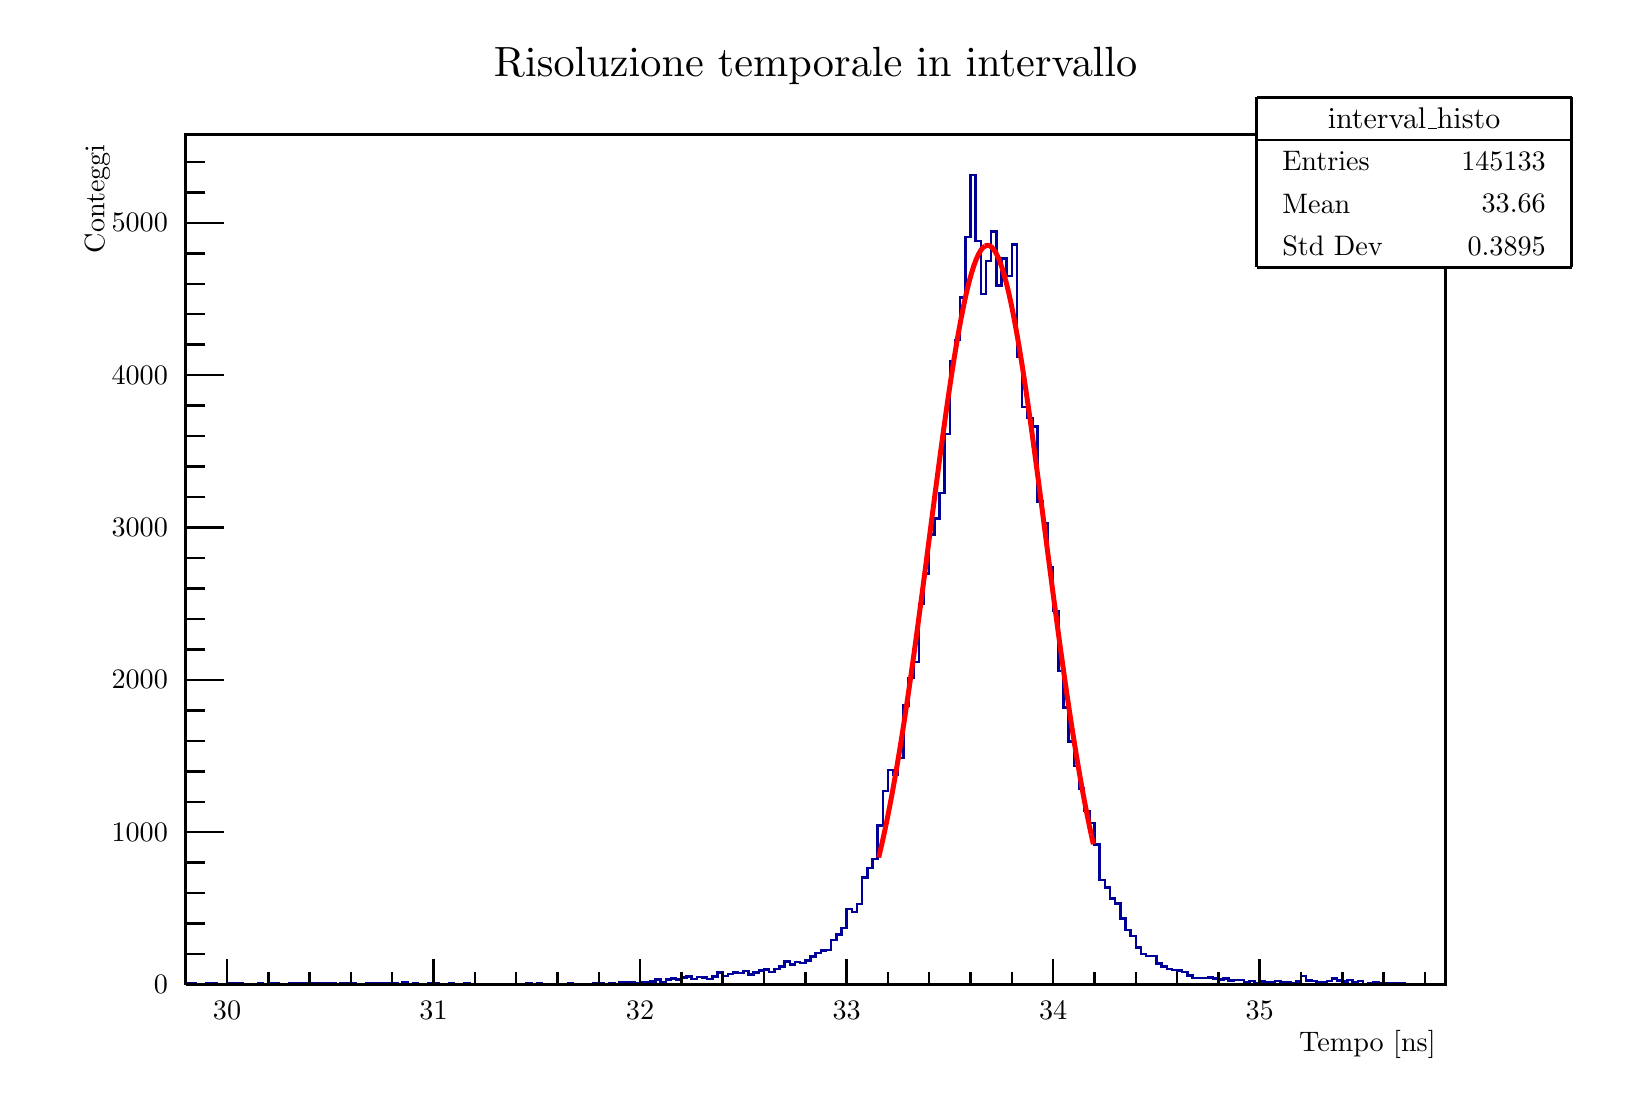
\begin{tikzpicture}
\pgfdeclareplotmark{cross} {
\pgfpathmoveto{\pgfpoint{-0.3\pgfplotmarksize}{\pgfplotmarksize}}
\pgfpathlineto{\pgfpoint{+0.3\pgfplotmarksize}{\pgfplotmarksize}}
\pgfpathlineto{\pgfpoint{+0.3\pgfplotmarksize}{0.3\pgfplotmarksize}}
\pgfpathlineto{\pgfpoint{+1\pgfplotmarksize}{0.3\pgfplotmarksize}}
\pgfpathlineto{\pgfpoint{+1\pgfplotmarksize}{-0.3\pgfplotmarksize}}
\pgfpathlineto{\pgfpoint{+0.3\pgfplotmarksize}{-0.3\pgfplotmarksize}}
\pgfpathlineto{\pgfpoint{+0.3\pgfplotmarksize}{-1.\pgfplotmarksize}}
\pgfpathlineto{\pgfpoint{-0.3\pgfplotmarksize}{-1.\pgfplotmarksize}}
\pgfpathlineto{\pgfpoint{-0.3\pgfplotmarksize}{-0.3\pgfplotmarksize}}
\pgfpathlineto{\pgfpoint{-1.\pgfplotmarksize}{-0.3\pgfplotmarksize}}
\pgfpathlineto{\pgfpoint{-1.\pgfplotmarksize}{0.3\pgfplotmarksize}}
\pgfpathlineto{\pgfpoint{-0.3\pgfplotmarksize}{0.3\pgfplotmarksize}}
\pgfpathclose
\pgfusepathqstroke
}
\pgfdeclareplotmark{cross*} {
\pgfpathmoveto{\pgfpoint{-0.3\pgfplotmarksize}{\pgfplotmarksize}}
\pgfpathlineto{\pgfpoint{+0.3\pgfplotmarksize}{\pgfplotmarksize}}
\pgfpathlineto{\pgfpoint{+0.3\pgfplotmarksize}{0.3\pgfplotmarksize}}
\pgfpathlineto{\pgfpoint{+1\pgfplotmarksize}{0.3\pgfplotmarksize}}
\pgfpathlineto{\pgfpoint{+1\pgfplotmarksize}{-0.3\pgfplotmarksize}}
\pgfpathlineto{\pgfpoint{+0.3\pgfplotmarksize}{-0.3\pgfplotmarksize}}
\pgfpathlineto{\pgfpoint{+0.3\pgfplotmarksize}{-1.\pgfplotmarksize}}
\pgfpathlineto{\pgfpoint{-0.3\pgfplotmarksize}{-1.\pgfplotmarksize}}
\pgfpathlineto{\pgfpoint{-0.3\pgfplotmarksize}{-0.3\pgfplotmarksize}}
\pgfpathlineto{\pgfpoint{-1.\pgfplotmarksize}{-0.3\pgfplotmarksize}}
\pgfpathlineto{\pgfpoint{-1.\pgfplotmarksize}{0.3\pgfplotmarksize}}
\pgfpathlineto{\pgfpoint{-0.3\pgfplotmarksize}{0.3\pgfplotmarksize}}
\pgfpathclose
\pgfusepathqfillstroke
}
\pgfdeclareplotmark{newstar} {
\pgfpathmoveto{\pgfqpoint{0pt}{\pgfplotmarksize}}
\pgfpathlineto{\pgfqpointpolar{44}{0.5\pgfplotmarksize}}
\pgfpathlineto{\pgfqpointpolar{18}{\pgfplotmarksize}}
\pgfpathlineto{\pgfqpointpolar{-20}{0.5\pgfplotmarksize}}
\pgfpathlineto{\pgfqpointpolar{-54}{\pgfplotmarksize}}
\pgfpathlineto{\pgfqpointpolar{-90}{0.5\pgfplotmarksize}}
\pgfpathlineto{\pgfqpointpolar{234}{\pgfplotmarksize}}
\pgfpathlineto{\pgfqpointpolar{198}{0.5\pgfplotmarksize}}
\pgfpathlineto{\pgfqpointpolar{162}{\pgfplotmarksize}}
\pgfpathlineto{\pgfqpointpolar{134}{0.5\pgfplotmarksize}}
\pgfpathclose
\pgfusepathqstroke
}
\pgfdeclareplotmark{newstar*} {
\pgfpathmoveto{\pgfqpoint{0pt}{\pgfplotmarksize}}
\pgfpathlineto{\pgfqpointpolar{44}{0.5\pgfplotmarksize}}
\pgfpathlineto{\pgfqpointpolar{18}{\pgfplotmarksize}}
\pgfpathlineto{\pgfqpointpolar{-20}{0.5\pgfplotmarksize}}
\pgfpathlineto{\pgfqpointpolar{-54}{\pgfplotmarksize}}
\pgfpathlineto{\pgfqpointpolar{-90}{0.5\pgfplotmarksize}}
\pgfpathlineto{\pgfqpointpolar{234}{\pgfplotmarksize}}
\pgfpathlineto{\pgfqpointpolar{198}{0.5\pgfplotmarksize}}
\pgfpathlineto{\pgfqpointpolar{162}{\pgfplotmarksize}}
\pgfpathlineto{\pgfqpointpolar{134}{0.5\pgfplotmarksize}}
\pgfpathclose
\pgfusepathqfillstroke
}
\definecolor{c}{rgb}{1,1,1};
\draw [color=c, fill=c] (0,0) rectangle (20,13.4957);
\draw [color=c, fill=c] (2,1.34957) rectangle (18,12.1461);
\definecolor{c}{rgb}{0,0,0};
\draw [c,line width=0.9] (2,1.34957) -- (2,12.1461) -- (18,12.1461) -- (18,1.34957) -- (2,1.34957);
\definecolor{c}{rgb}{1,1,1};
\draw [color=c, fill=c] (2,1.34957) rectangle (18,12.1461);
\definecolor{c}{rgb}{0,0,0};
\draw [c,line width=0.9] (2,1.34957) -- (2,12.1461) -- (18,12.1461) -- (18,1.34957) -- (2,1.34957);
\definecolor{c}{rgb}{0,0,0.6};
\draw [c,line width=0.9] (2,1.36118) -- (2.06557,1.36118) -- (2.06557,1.36698) -- (2.13115,1.36698) -- (2.13115,1.35344) -- (2.19672,1.35344) -- (2.19672,1.35538) -- (2.2623,1.35538) -- (2.2623,1.36118) -- (2.32787,1.36118) -- (2.32787,1.36118) --
 (2.39344,1.36118) -- (2.39344,1.35151) -- (2.45902,1.35151) -- (2.45902,1.35731) -- (2.52459,1.35731) -- (2.52459,1.36698) -- (2.59016,1.36698) -- (2.59016,1.36698) -- (2.65574,1.36698) -- (2.65574,1.36505) -- (2.72131,1.36505) -- (2.72131,1.35731)
 -- (2.78689,1.35731) -- (2.78689,1.35538) -- (2.85246,1.35538) -- (2.85246,1.35731) -- (2.91803,1.35731) -- (2.91803,1.36892) -- (2.98361,1.36892) -- (2.98361,1.35925) -- (3.04918,1.35925) -- (3.04918,1.37085) -- (3.11475,1.37085) --
 (3.11475,1.36698) -- (3.18033,1.36698) -- (3.18033,1.35538) -- (3.2459,1.35538) -- (3.2459,1.35731) -- (3.31148,1.35731) -- (3.31148,1.36118) -- (3.37705,1.36118) -- (3.37705,1.36892) -- (3.44262,1.36892) -- (3.44262,1.36698) -- (3.5082,1.36698) --
 (3.5082,1.36118) -- (3.57377,1.36118) -- (3.57377,1.36505) -- (3.63934,1.36505) -- (3.63934,1.37085) -- (3.70492,1.37085) -- (3.70492,1.36698) -- (3.77049,1.36698) -- (3.77049,1.36312) -- (3.83607,1.36312) -- (3.83607,1.36312) -- (3.90164,1.36312)
 -- (3.90164,1.35538) -- (3.96721,1.35538) -- (3.96721,1.36118) -- (4.03279,1.36118) -- (4.03279,1.36698) -- (4.09836,1.36698) -- (4.09836,1.36312) -- (4.16393,1.36312) -- (4.16393,1.35731) -- (4.22951,1.35731) -- (4.22951,1.35925) --
 (4.29508,1.35925) -- (4.29508,1.36505) -- (4.36066,1.36505) -- (4.36066,1.36118) -- (4.42623,1.36118) -- (4.42623,1.36312) -- (4.4918,1.36312) -- (4.4918,1.36118) -- (4.55738,1.36118) -- (4.55738,1.36312) -- (4.62295,1.36312) -- (4.62295,1.36312) --
 (4.68852,1.36312) -- (4.68852,1.35538) -- (4.7541,1.35538) -- (4.7541,1.37472) -- (4.81967,1.37472) -- (4.81967,1.35731) -- (4.88525,1.35731) -- (4.88525,1.36892) -- (4.95082,1.36892) -- (4.95082,1.35925) -- (5.01639,1.35925) -- (5.01639,1.35538) --
 (5.08197,1.35538) -- (5.08197,1.36312) -- (5.14754,1.36312) -- (5.14754,1.36505) -- (5.21311,1.36505) -- (5.21311,1.35925) -- (5.27869,1.35925) -- (5.27869,1.35538) -- (5.34426,1.35538) -- (5.34426,1.36505) -- (5.40984,1.36505) -- (5.40984,1.34957)
 -- (5.47541,1.34957) -- (5.47541,1.35731) -- (5.54098,1.35731) -- (5.54098,1.36505) -- (5.60656,1.36505) -- (5.60656,1.35731) -- (5.67213,1.35731) -- (5.67213,1.35538) -- (5.7377,1.35538) -- (5.7377,1.35925) -- (5.80328,1.35925) -- (5.80328,1.35538)
 -- (5.86885,1.35538) -- (5.86885,1.35344) -- (5.93443,1.35344) -- (5.93443,1.35731) -- (6,1.35731) -- (6,1.35344) -- (6.06557,1.35344) -- (6.06557,1.35151) -- (6.13115,1.35151) -- (6.13115,1.35925) -- (6.19672,1.35925) -- (6.19672,1.35538) --
 (6.2623,1.35538) -- (6.2623,1.35538) -- (6.32787,1.35538) -- (6.32787,1.36118) -- (6.39344,1.36118) -- (6.39344,1.35925) -- (6.45902,1.35925) -- (6.45902,1.36312) -- (6.52459,1.36312) -- (6.52459,1.35538) -- (6.59016,1.35538) -- (6.59016,1.35925) --
 (6.65574,1.35925) -- (6.65574,1.35731) -- (6.72131,1.35731) -- (6.72131,1.35731) -- (6.78689,1.35731) -- (6.78689,1.35344) -- (6.85246,1.35344) -- (6.85246,1.36312) -- (6.91803,1.36312) -- (6.91803,1.35731) -- (6.98361,1.35731) -- (6.98361,1.35344)
 -- (7.04918,1.35344) -- (7.04918,1.35731) -- (7.11475,1.35731) -- (7.11475,1.35925) -- (7.18033,1.35925) -- (7.18033,1.36118) -- (7.2459,1.36118) -- (7.2459,1.36118) -- (7.31148,1.36118) -- (7.31148,1.35925) -- (7.37705,1.35925) -- (7.37705,1.36698)
 -- (7.44262,1.36698) -- (7.44262,1.35731) -- (7.5082,1.35731) -- (7.5082,1.37666) -- (7.57377,1.37666) -- (7.57377,1.37666) -- (7.63934,1.37666) -- (7.63934,1.38246) -- (7.70492,1.38246) -- (7.70492,1.36698) -- (7.77049,1.36698) -- (7.77049,1.37859)
 -- (7.83607,1.37859) -- (7.83607,1.37859) -- (7.90164,1.37859) -- (7.90164,1.38633) -- (7.96721,1.38633) -- (7.96721,1.41149) -- (8.03279,1.41149) -- (8.03279,1.38053) -- (8.09836,1.38053) -- (8.09836,1.41729) -- (8.16393,1.41729) --
 (8.16393,1.4289) -- (8.22951,1.4289) -- (8.22951,1.41536) -- (8.29508,1.41536) -- (8.29508,1.43858) -- (8.36066,1.43858) -- (8.36066,1.45019) -- (8.42623,1.45019) -- (8.42623,1.4231) -- (8.4918,1.4231) -- (8.4918,1.44632) -- (8.55738,1.44632) --
 (8.55738,1.43858) -- (8.62295,1.43858) -- (8.62295,1.41923) -- (8.68852,1.41923) -- (8.68852,1.45212) -- (8.7541,1.45212) -- (8.7541,1.5005) -- (8.81967,1.5005) -- (8.81967,1.45986) -- (8.88525,1.45986) -- (8.88525,1.48502) -- (8.95082,1.48502) --
 (8.95082,1.50243) -- (9.01639,1.50243) -- (9.01639,1.49469) -- (9.08197,1.49469) -- (9.08197,1.52178) -- (9.14754,1.52178) -- (9.14754,1.47921) -- (9.21311,1.47921) -- (9.21311,1.5063) -- (9.27869,1.5063) -- (9.27869,1.52952) -- (9.34426,1.52952) --
 (9.34426,1.5392) -- (9.40984,1.5392) -- (9.40984,1.51211) -- (9.47541,1.51211) -- (9.47541,1.54694) -- (9.54098,1.54694) -- (9.54098,1.58177) -- (9.60656,1.58177) -- (9.60656,1.64175) -- (9.67213,1.64175) -- (9.67213,1.60499) -- (9.73771,1.60499) --
 (9.73771,1.63982) -- (9.80328,1.63982) -- (9.80328,1.6224) -- (9.86885,1.6224) -- (9.86885,1.65723) -- (9.93443,1.65723) -- (9.93443,1.70561) -- (10,1.70561) -- (10,1.75204) -- (10.0656,1.75204) -- (10.0656,1.78107) -- (10.1311,1.78107) --
 (10.1311,1.78881) -- (10.1967,1.78881) -- (10.1967,1.91652) -- (10.2623,1.91652) -- (10.2623,1.98424) -- (10.3279,1.98424) -- (10.3279,2.06551) -- (10.3934,2.06551) -- (10.3934,2.30738) -- (10.459,2.30738) -- (10.459,2.27062) -- (10.5246,2.27062) --
 (10.5246,2.37124) -- (10.5902,2.37124) -- (10.5902,2.70986) -- (10.6557,2.70986) -- (10.6557,2.82982) -- (10.7213,2.82982) -- (10.7213,2.94399) -- (10.7869,2.94399) -- (10.7869,3.36775) -- (10.8525,3.36775) -- (10.8525,3.81085) -- (10.918,3.81085)
 -- (10.918,4.07595) -- (10.9836,4.07595) -- (10.9836,4.01596) -- (11.0492,4.01596) -- (11.0492,4.22881) -- (11.1148,4.22881) -- (11.1148,4.89637) -- (11.1803,4.89637) -- (11.1803,5.2466) -- (11.2459,5.2466) -- (11.2459,5.44784) -- (11.3115,5.44784)
 -- (11.3115,6.18506) -- (11.377,6.18506) -- (11.377,6.57206) -- (11.4426,6.57206) -- (11.4426,7.06354) -- (11.5082,7.06354) -- (11.5082,7.26671) -- (11.5738,7.26671) -- (11.5738,7.59566) -- (11.6393,7.59566) -- (11.6393,8.34449) -- (11.7049,8.34449)
 -- (11.7049,9.26167) -- (11.7705,9.26167) -- (11.7705,9.53644) -- (11.8361,9.53644) -- (11.8361,10.0763) -- (11.9016,10.0763) -- (11.9016,10.8445) -- (11.9672,10.8445) -- (11.9672,11.632) -- (12.0328,11.632) -- (12.0328,10.7961) -- (12.0984,10.7961)
 -- (12.0984,10.1227) -- (12.1639,10.1227) -- (12.1639,10.5368) -- (12.2295,10.5368) -- (12.2295,10.9141) -- (12.2951,10.9141) -- (12.2951,10.2292) -- (12.3607,10.2292) -- (12.3607,10.5697) -- (12.4262,10.5697) -- (12.4262,10.3511) --
 (12.4918,10.3511) -- (12.4918,10.7497) -- (12.5574,10.7497) -- (12.5574,9.32746) -- (12.623,9.32746) -- (12.623,8.68505) -- (12.6885,8.68505) -- (12.6885,8.54766) -- (12.7541,8.54766) -- (12.7541,8.43931) -- (12.8197,8.43931) -- (12.8197,7.48343) --
 (12.8852,7.48343) -- (12.8852,7.20673) -- (12.9508,7.20673) -- (12.9508,6.65333) -- (13.0164,6.65333) -- (13.0164,6.09412) -- (13.082,6.09412) -- (13.082,5.33368) -- (13.1475,5.33368) -- (13.1475,4.87122) -- (13.2131,4.87122) -- (13.2131,4.43972) --
 (13.2787,4.43972) -- (13.2787,4.12819) -- (13.3443,4.12819) -- (13.3443,3.84181) -- (13.4098,3.84181) -- (13.4098,3.55157) -- (13.4754,3.55157) -- (13.4754,3.40064) -- (13.541,3.40064) -- (13.541,3.13168) -- (13.6066,3.13168) -- (13.6066,2.6789) --
 (13.6721,2.6789) -- (13.6721,2.58602) -- (13.7377,2.58602) -- (13.7377,2.44476) -- (13.8033,2.44476) -- (13.8033,2.37898) -- (13.8689,2.37898) -- (13.8689,2.18741) -- (13.9344,2.18741) -- (13.9344,2.04229) -- (14,2.04229) -- (14,1.96489) --
 (14.0656,1.96489) -- (14.0656,1.81977) -- (14.1311,1.81977) -- (14.1311,1.7385) -- (14.1967,1.7385) -- (14.1967,1.71528) -- (14.2623,1.71528) -- (14.2623,1.71334) -- (14.3279,1.71334) -- (14.3279,1.6166) -- (14.3934,1.6166) -- (14.3934,1.58177) --
 (14.459,1.58177) -- (14.459,1.545) -- (14.5246,1.545) -- (14.5246,1.53533) -- (14.5902,1.53533) -- (14.5902,1.52952) -- (14.6557,1.52952) -- (14.6557,1.51017) -- (14.7213,1.51017) -- (14.7213,1.4676) -- (14.7869,1.4676) -- (14.7869,1.43664) --
 (14.8525,1.43664) -- (14.8525,1.43277) -- (14.918,1.43277) -- (14.918,1.43471) -- (14.9836,1.43471) -- (14.9836,1.44245) -- (15.0492,1.44245) -- (15.0492,1.42503) -- (15.1148,1.42503) -- (15.1148,1.41342) -- (15.1803,1.41342) -- (15.1803,1.42697) --
 (15.2459,1.42697) -- (15.2459,1.39988) -- (15.3115,1.39988) -- (15.3115,1.40762) -- (15.377,1.40762) -- (15.377,1.40762) -- (15.4426,1.40762) -- (15.4426,1.37859) -- (15.5082,1.37859) -- (15.5082,1.39407) -- (15.5738,1.39407) -- (15.5738,1.36698) --
 (15.6393,1.36698) -- (15.6393,1.38633) -- (15.7049,1.38633) -- (15.7049,1.38053) -- (15.7705,1.38053) -- (15.7705,1.37472) -- (15.8361,1.37472) -- (15.8361,1.39601) -- (15.9016,1.39601) -- (15.9016,1.38246) -- (15.9672,1.38246) -- (15.9672,1.38246)
 -- (16.0328,1.38246) -- (16.0328,1.37279) -- (16.0984,1.37279) -- (16.0984,1.38827) -- (16.1639,1.38827) -- (16.1639,1.45793) -- (16.2295,1.45793) -- (16.2295,1.40181) -- (16.2951,1.40181) -- (16.2951,1.39794) -- (16.3607,1.39794) --
 (16.3607,1.37859) -- (16.4262,1.37859) -- (16.4262,1.38246) -- (16.4918,1.38246) -- (16.4918,1.39794) -- (16.5574,1.39794) -- (16.5574,1.42503) -- (16.623,1.42503) -- (16.623,1.39988) -- (16.6885,1.39988) -- (16.6885,1.38633) -- (16.7541,1.38633) --
 (16.7541,1.40955) -- (16.8197,1.40955) -- (16.8197,1.38053) -- (16.8852,1.38053) -- (16.8852,1.39794) -- (16.9508,1.39794) -- (16.9508,1.35925) -- (17.0164,1.35925) -- (17.0164,1.37085) -- (17.082,1.37085) -- (17.082,1.38053) -- (17.1475,1.38053) --
 (17.1475,1.37279) -- (17.2131,1.37279) -- (17.2131,1.37279) -- (17.2787,1.37279) -- (17.2787,1.36118) -- (17.3443,1.36118) -- (17.3443,1.36312) -- (17.4098,1.36312) -- (17.4098,1.36118) -- (17.4754,1.36118) -- (17.4754,1.35925) -- (17.541,1.35925)
 -- (17.541,1.35731) -- (17.6066,1.35731) -- (17.6066,1.35344) -- (17.6721,1.35344) -- (17.6721,1.34957) -- (17.7377,1.34957) -- (17.7377,1.35731) -- (17.8033,1.35731) -- (17.8033,1.35151) -- (17.8689,1.35151) -- (17.8689,1.34957) --
 (17.9344,1.34957) -- (17.9344,1.34957) -- (18,1.34957);
\definecolor{c}{rgb}{1,1,1};
\draw [color=c, fill=c] (15.6,10.4592) rectangle (19.6,12.6185);
\definecolor{c}{rgb}{0,0,0};
\draw [c,line width=0.9] (15.6,10.4592) -- (19.6,10.4592);
\draw [c,line width=0.9] (19.6,10.4592) -- (19.6,12.6185);
\draw [c,line width=0.9] (19.6,12.6185) -- (15.6,12.6185);
\draw [c,line width=0.9] (15.6,12.6185) -- (15.6,10.4592);
\draw (17.6,12.3486) node[scale=1.08185, color=c, rotate=0]{interval\_histo};
\draw [c,line width=0.9] (15.6,12.0787) -- (19.6,12.0787);
\draw [anchor= west] (15.8,11.8087) node[scale=1.01821, color=c, rotate=0]{Entries };
\draw [anchor= east] (19.4,11.8087) node[scale=1.01821, color=c, rotate=0]{ 145133};
\draw [anchor= west] (15.8,11.2689) node[scale=1.01821, color=c, rotate=0]{Mean  };
\draw [anchor= east] (19.4,11.2689) node[scale=1.01821, color=c, rotate=0]{  33.66};
\draw [anchor= west] (15.8,10.7291) node[scale=1.01821, color=c, rotate=0]{Std Dev   };
\draw [anchor= east] (19.4,10.7291) node[scale=1.01821, color=c, rotate=0]{ 0.3895};
\definecolor{c}{rgb}{1,0,0};
\draw [c,line width=1.8] (10.8007,2.96365) -- (10.8282,3.0797) -- (10.8557,3.2015) -- (10.8833,3.3291) -- (10.9108,3.46255) -- (10.9384,3.60185) -- (10.9659,3.74698) -- (10.9934,3.89789) -- (11.021,4.05453) -- (11.0485,4.21679) -- (11.0761,4.38455)
 -- (11.1036,4.55763) -- (11.1311,4.73586) -- (11.1587,4.919) -- (11.1862,5.10679) -- (11.2138,5.29894) -- (11.2413,5.49513) -- (11.2689,5.69499) -- (11.2964,5.89813) -- (11.3239,6.10413) -- (11.3515,6.31251) -- (11.379,6.5228) -- (11.4066,6.73448)
 -- (11.4341,6.94699) -- (11.4616,7.15978) -- (11.4892,7.37224) -- (11.5167,7.58375) -- (11.5443,7.79369) -- (11.5718,8.0014) -- (11.5993,8.20622) -- (11.6269,8.40749) -- (11.6544,8.60453) -- (11.682,8.79667) -- (11.7095,8.98322) -- (11.737,9.16353)
 -- (11.7646,9.33694) -- (11.7921,9.5028) -- (11.8197,9.66049) -- (11.8472,9.80941) -- (11.8748,9.94898) -- (11.9023,10.0787) -- (11.9298,10.1979) -- (11.9574,10.3063) -- (11.9849,10.4034) -- (12.0125,10.4887) -- (12.04,10.562) -- (12.0675,10.6229)
 -- (12.0951,10.6711) -- (12.1226,10.7066) -- (12.1502,10.7291);
\draw [c,line width=1.8] (12.1502,10.7291) -- (12.1777,10.7385) -- (12.2052,10.7348) -- (12.2328,10.718) -- (12.2603,10.6882) -- (12.2879,10.6455) -- (12.3154,10.5901) -- (12.343,10.5222) -- (12.3705,10.4421) -- (12.398,10.3501) -- (12.4256,10.2466)
 -- (12.4531,10.132) -- (12.4807,10.0068) -- (12.5082,9.8715) -- (12.5357,9.72659) -- (12.5633,9.57265) -- (12.5908,9.41028) -- (12.6184,9.24009) -- (12.6459,9.06271) -- (12.6734,8.8788) -- (12.701,8.68902) -- (12.7285,8.49404) -- (12.7561,8.29453)
 -- (12.7836,8.09117) -- (12.8111,7.88464) -- (12.8387,7.67559) -- (12.8662,7.46469) -- (12.8938,7.25257) -- (12.9213,7.03985) -- (12.9489,6.82715) -- (12.9764,6.61504) -- (13.0039,6.40407) -- (13.0315,6.1948) -- (13.059,5.9877) -- (13.0866,5.78326)
 -- (13.1141,5.58192) -- (13.1416,5.38408) -- (13.1692,5.19012) -- (13.1967,5.00039) -- (13.2243,4.81519) -- (13.2518,4.63479) -- (13.2793,4.45944) -- (13.3069,4.28933) -- (13.3344,4.12466) -- (13.362,3.96555) -- (13.3895,3.81212) -- (13.417,3.66446)
 -- (13.4446,3.52262) -- (13.4721,3.38662) -- (13.4997,3.25647);
\draw [c,line width=1.8] (13.4997,3.25647) -- (13.5272,3.13214);
\definecolor{c}{rgb}{0,0,0};
\draw [c,line width=0.9] (2,1.34957) -- (18,1.34957);
\draw [anchor= east] (18,0.593811) node[scale=1.01821, color=c, rotate=0]{Tempo [ns]};
\draw [c,line width=0.9] (2.52459,1.67347) -- (2.52459,1.34957);
\draw [c,line width=0.9] (3.04918,1.51152) -- (3.04918,1.34957);
\draw [c,line width=0.9] (3.57377,1.51152) -- (3.57377,1.34957);
\draw [c,line width=0.9] (4.09836,1.51152) -- (4.09836,1.34957);
\draw [c,line width=0.9] (4.62295,1.51152) -- (4.62295,1.34957);
\draw [c,line width=0.9] (5.14754,1.67347) -- (5.14754,1.34957);
\draw [c,line width=0.9] (5.67213,1.51152) -- (5.67213,1.34957);
\draw [c,line width=0.9] (6.19672,1.51152) -- (6.19672,1.34957);
\draw [c,line width=0.9] (6.72131,1.51152) -- (6.72131,1.34957);
\draw [c,line width=0.9] (7.2459,1.51152) -- (7.2459,1.34957);
\draw [c,line width=0.9] (7.77049,1.67347) -- (7.77049,1.34957);
\draw [c,line width=0.9] (8.29508,1.51152) -- (8.29508,1.34957);
\draw [c,line width=0.9] (8.81967,1.51152) -- (8.81967,1.34957);
\draw [c,line width=0.9] (9.34426,1.51152) -- (9.34426,1.34957);
\draw [c,line width=0.9] (9.86885,1.51152) -- (9.86885,1.34957);
\draw [c,line width=0.9] (10.3934,1.67347) -- (10.3934,1.34957);
\draw [c,line width=0.9] (10.918,1.51152) -- (10.918,1.34957);
\draw [c,line width=0.9] (11.4426,1.51152) -- (11.4426,1.34957);
\draw [c,line width=0.9] (11.9672,1.51152) -- (11.9672,1.34957);
\draw [c,line width=0.9] (12.4918,1.51152) -- (12.4918,1.34957);
\draw [c,line width=0.9] (13.0164,1.67347) -- (13.0164,1.34957);
\draw [c,line width=0.9] (13.541,1.51152) -- (13.541,1.34957);
\draw [c,line width=0.9] (14.0656,1.51152) -- (14.0656,1.34957);
\draw [c,line width=0.9] (14.5902,1.51152) -- (14.5902,1.34957);
\draw [c,line width=0.9] (15.1148,1.51152) -- (15.1148,1.34957);
\draw [c,line width=0.9] (15.6393,1.67347) -- (15.6393,1.34957);
\draw [c,line width=0.9] (2.52459,1.67347) -- (2.52459,1.34957);
\draw [c,line width=0.9] (15.6393,1.67347) -- (15.6393,1.34957);
\draw [c,line width=0.9] (16.1639,1.51152) -- (16.1639,1.34957);
\draw [c,line width=0.9] (16.6885,1.51152) -- (16.6885,1.34957);
\draw [c,line width=0.9] (17.2131,1.51152) -- (17.2131,1.34957);
\draw [c,line width=0.9] (17.7377,1.51152) -- (17.7377,1.34957);
\draw [anchor=base] (2.52459,0.904212) node[scale=1.01821, color=c, rotate=0]{30};
\draw [anchor=base] (5.14754,0.904212) node[scale=1.01821, color=c, rotate=0]{31};
\draw [anchor=base] (7.77049,0.904212) node[scale=1.01821, color=c, rotate=0]{32};
\draw [anchor=base] (10.3934,0.904212) node[scale=1.01821, color=c, rotate=0]{33};
\draw [anchor=base] (13.0164,0.904212) node[scale=1.01821, color=c, rotate=0]{34};
\draw [anchor=base] (15.6393,0.904212) node[scale=1.01821, color=c, rotate=0]{35};
\draw [c,line width=0.9] (2,1.34957) -- (2,12.1461);
\draw [anchor= east] (0.88,12.1461) node[scale=1.01821, color=c, rotate=90]{Conteggi};
\draw [c,line width=0.9] (2.48,1.34957) -- (2,1.34957);
\draw [c,line width=0.9] (2.24,1.73656) -- (2,1.73656);
\draw [c,line width=0.9] (2.24,2.12356) -- (2,2.12356);
\draw [c,line width=0.9] (2.24,2.51055) -- (2,2.51055);
\draw [c,line width=0.9] (2.24,2.89755) -- (2,2.89755);
\draw [c,line width=0.9] (2.48,3.28454) -- (2,3.28454);
\draw [c,line width=0.9] (2.24,3.67154) -- (2,3.67154);
\draw [c,line width=0.9] (2.24,4.05853) -- (2,4.05853);
\draw [c,line width=0.9] (2.24,4.44552) -- (2,4.44552);
\draw [c,line width=0.9] (2.24,4.83252) -- (2,4.83252);
\draw [c,line width=0.9] (2.48,5.21951) -- (2,5.21951);
\draw [c,line width=0.9] (2.24,5.60651) -- (2,5.60651);
\draw [c,line width=0.9] (2.24,5.9935) -- (2,5.9935);
\draw [c,line width=0.9] (2.24,6.3805) -- (2,6.3805);
\draw [c,line width=0.9] (2.24,6.76749) -- (2,6.76749);
\draw [c,line width=0.9] (2.48,7.15449) -- (2,7.15449);
\draw [c,line width=0.9] (2.24,7.54148) -- (2,7.54148);
\draw [c,line width=0.9] (2.24,7.92847) -- (2,7.92847);
\draw [c,line width=0.9] (2.24,8.31547) -- (2,8.31547);
\draw [c,line width=0.9] (2.24,8.70246) -- (2,8.70246);
\draw [c,line width=0.9] (2.48,9.08946) -- (2,9.08946);
\draw [c,line width=0.9] (2.24,9.47645) -- (2,9.47645);
\draw [c,line width=0.9] (2.24,9.86345) -- (2,9.86345);
\draw [c,line width=0.9] (2.24,10.2504) -- (2,10.2504);
\draw [c,line width=0.9] (2.24,10.6374) -- (2,10.6374);
\draw [c,line width=0.9] (2.48,11.0244) -- (2,11.0244);
\draw [c,line width=0.9] (2.48,11.0244) -- (2,11.0244);
\draw [c,line width=0.9] (2.24,11.4114) -- (2,11.4114);
\draw [c,line width=0.9] (2.24,11.7984) -- (2,11.7984);
\draw [anchor= east] (1.9,1.34957) node[scale=1.01821, color=c, rotate=0]{0};
\draw [anchor= east] (1.9,3.28454) node[scale=1.01821, color=c, rotate=0]{1000};
\draw [anchor= east] (1.9,5.21951) node[scale=1.01821, color=c, rotate=0]{2000};
\draw [anchor= east] (1.9,7.15449) node[scale=1.01821, color=c, rotate=0]{3000};
\draw [anchor= east] (1.9,9.08946) node[scale=1.01821, color=c, rotate=0]{4000};
\draw [anchor= east] (1.9,11.0244) node[scale=1.01821, color=c, rotate=0]{5000};
\definecolor{c}{rgb}{1,1,1};
\draw [color=c, fill=c] (15.6,10.4592) rectangle (19.6,12.6185);
\definecolor{c}{rgb}{0,0,0};
\draw [c,line width=0.9] (15.6,10.4592) -- (19.6,10.4592);
\draw [c,line width=0.9] (19.6,10.4592) -- (19.6,12.6185);
\draw [c,line width=0.9] (19.6,12.6185) -- (15.6,12.6185);
\draw [c,line width=0.9] (15.6,12.6185) -- (15.6,10.4592);
\draw (17.6,12.3486) node[scale=1.08185, color=c, rotate=0]{interval\_histo};
\draw [c,line width=0.9] (15.6,12.0787) -- (19.6,12.0787);
\draw [anchor= west] (15.8,11.8087) node[scale=1.01821, color=c, rotate=0]{Entries };
\draw [anchor= east] (19.4,11.8087) node[scale=1.01821, color=c, rotate=0]{ 145133};
\draw [anchor= west] (15.8,11.2689) node[scale=1.01821, color=c, rotate=0]{Mean  };
\draw [anchor= east] (19.4,11.2689) node[scale=1.01821, color=c, rotate=0]{  33.66};
\draw [anchor= west] (15.8,10.7291) node[scale=1.01821, color=c, rotate=0]{Std Dev   };
\draw [anchor= east] (19.4,10.7291) node[scale=1.01821, color=c, rotate=0]{ 0.3895};
\draw (10,13.0156) node[scale=1.52731, color=c, rotate=0]{Risoluzione temporale in intervallo};
\end{tikzpicture}

%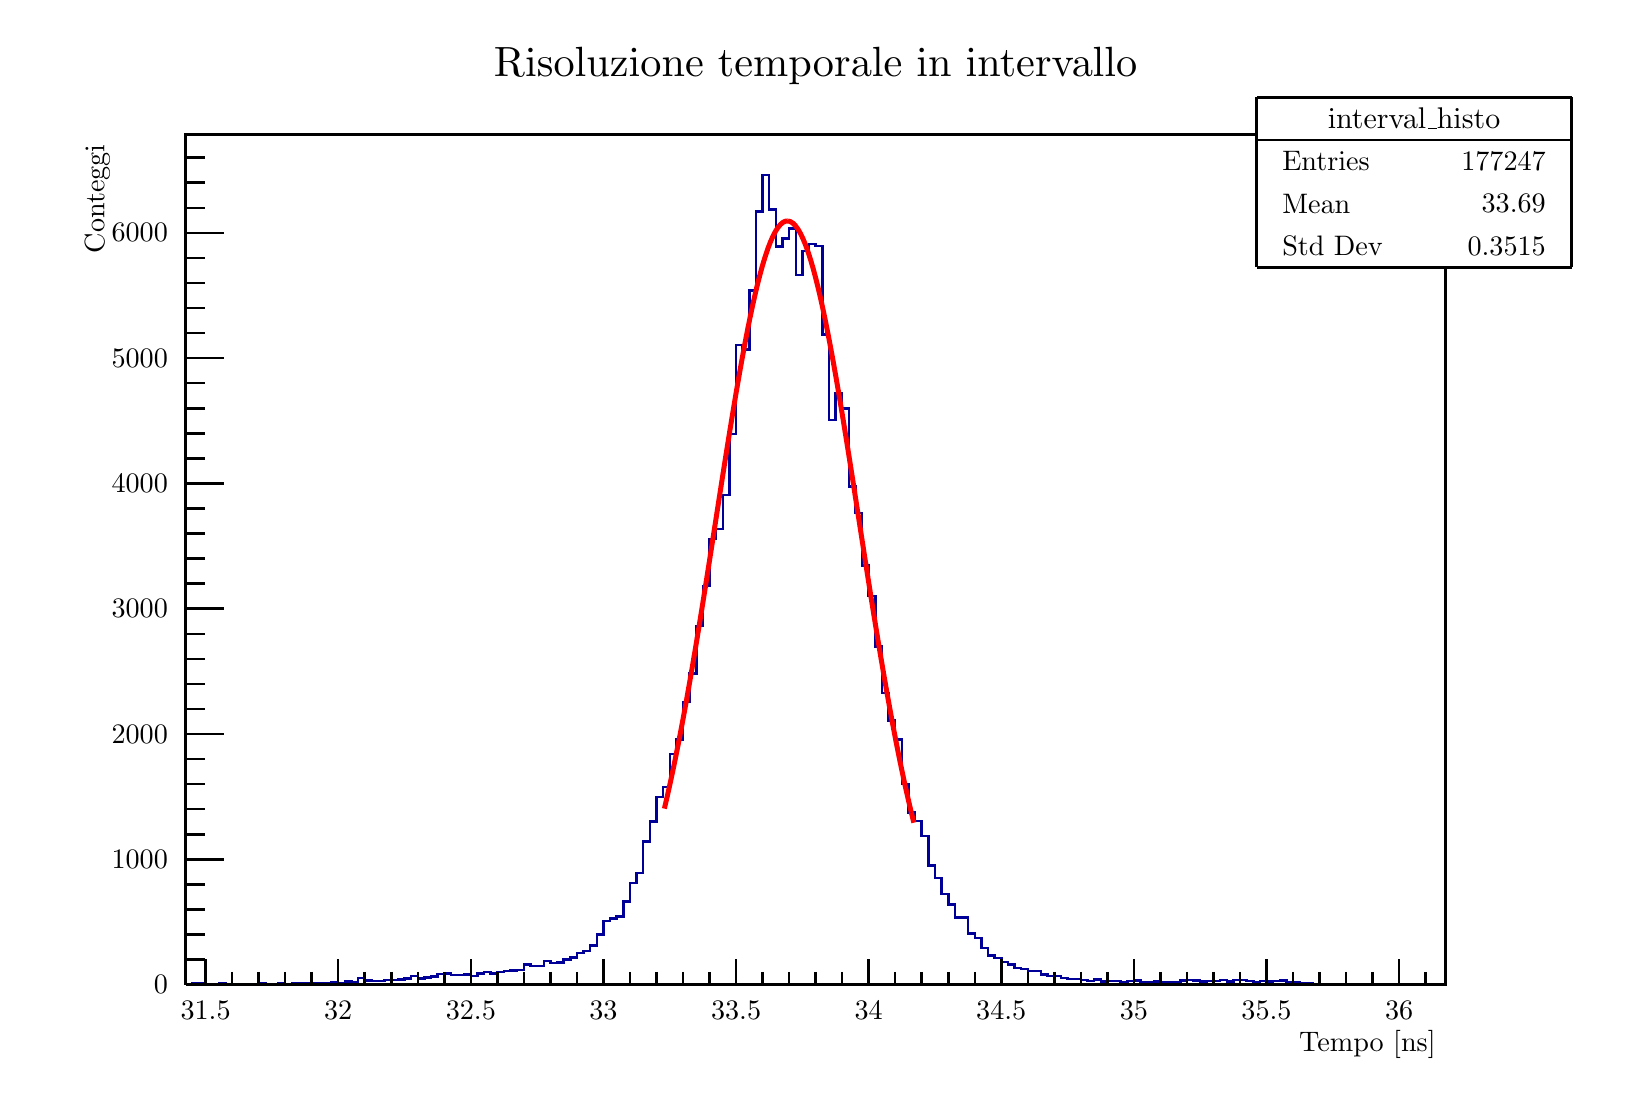
\begin{tikzpicture}
\pgfdeclareplotmark{cross} {
\pgfpathmoveto{\pgfpoint{-0.3\pgfplotmarksize}{\pgfplotmarksize}}
\pgfpathlineto{\pgfpoint{+0.3\pgfplotmarksize}{\pgfplotmarksize}}
\pgfpathlineto{\pgfpoint{+0.3\pgfplotmarksize}{0.3\pgfplotmarksize}}
\pgfpathlineto{\pgfpoint{+1\pgfplotmarksize}{0.3\pgfplotmarksize}}
\pgfpathlineto{\pgfpoint{+1\pgfplotmarksize}{-0.3\pgfplotmarksize}}
\pgfpathlineto{\pgfpoint{+0.3\pgfplotmarksize}{-0.3\pgfplotmarksize}}
\pgfpathlineto{\pgfpoint{+0.3\pgfplotmarksize}{-1.\pgfplotmarksize}}
\pgfpathlineto{\pgfpoint{-0.3\pgfplotmarksize}{-1.\pgfplotmarksize}}
\pgfpathlineto{\pgfpoint{-0.3\pgfplotmarksize}{-0.3\pgfplotmarksize}}
\pgfpathlineto{\pgfpoint{-1.\pgfplotmarksize}{-0.3\pgfplotmarksize}}
\pgfpathlineto{\pgfpoint{-1.\pgfplotmarksize}{0.3\pgfplotmarksize}}
\pgfpathlineto{\pgfpoint{-0.3\pgfplotmarksize}{0.3\pgfplotmarksize}}
\pgfpathclose
\pgfusepathqstroke
}
\pgfdeclareplotmark{cross*} {
\pgfpathmoveto{\pgfpoint{-0.3\pgfplotmarksize}{\pgfplotmarksize}}
\pgfpathlineto{\pgfpoint{+0.3\pgfplotmarksize}{\pgfplotmarksize}}
\pgfpathlineto{\pgfpoint{+0.3\pgfplotmarksize}{0.3\pgfplotmarksize}}
\pgfpathlineto{\pgfpoint{+1\pgfplotmarksize}{0.3\pgfplotmarksize}}
\pgfpathlineto{\pgfpoint{+1\pgfplotmarksize}{-0.3\pgfplotmarksize}}
\pgfpathlineto{\pgfpoint{+0.3\pgfplotmarksize}{-0.3\pgfplotmarksize}}
\pgfpathlineto{\pgfpoint{+0.3\pgfplotmarksize}{-1.\pgfplotmarksize}}
\pgfpathlineto{\pgfpoint{-0.3\pgfplotmarksize}{-1.\pgfplotmarksize}}
\pgfpathlineto{\pgfpoint{-0.3\pgfplotmarksize}{-0.3\pgfplotmarksize}}
\pgfpathlineto{\pgfpoint{-1.\pgfplotmarksize}{-0.3\pgfplotmarksize}}
\pgfpathlineto{\pgfpoint{-1.\pgfplotmarksize}{0.3\pgfplotmarksize}}
\pgfpathlineto{\pgfpoint{-0.3\pgfplotmarksize}{0.3\pgfplotmarksize}}
\pgfpathclose
\pgfusepathqfillstroke
}
\pgfdeclareplotmark{newstar} {
\pgfpathmoveto{\pgfqpoint{0pt}{\pgfplotmarksize}}
\pgfpathlineto{\pgfqpointpolar{44}{0.5\pgfplotmarksize}}
\pgfpathlineto{\pgfqpointpolar{18}{\pgfplotmarksize}}
\pgfpathlineto{\pgfqpointpolar{-20}{0.5\pgfplotmarksize}}
\pgfpathlineto{\pgfqpointpolar{-54}{\pgfplotmarksize}}
\pgfpathlineto{\pgfqpointpolar{-90}{0.5\pgfplotmarksize}}
\pgfpathlineto{\pgfqpointpolar{234}{\pgfplotmarksize}}
\pgfpathlineto{\pgfqpointpolar{198}{0.5\pgfplotmarksize}}
\pgfpathlineto{\pgfqpointpolar{162}{\pgfplotmarksize}}
\pgfpathlineto{\pgfqpointpolar{134}{0.5\pgfplotmarksize}}
\pgfpathclose
\pgfusepathqstroke
}
\pgfdeclareplotmark{newstar*} {
\pgfpathmoveto{\pgfqpoint{0pt}{\pgfplotmarksize}}
\pgfpathlineto{\pgfqpointpolar{44}{0.5\pgfplotmarksize}}
\pgfpathlineto{\pgfqpointpolar{18}{\pgfplotmarksize}}
\pgfpathlineto{\pgfqpointpolar{-20}{0.5\pgfplotmarksize}}
\pgfpathlineto{\pgfqpointpolar{-54}{\pgfplotmarksize}}
\pgfpathlineto{\pgfqpointpolar{-90}{0.5\pgfplotmarksize}}
\pgfpathlineto{\pgfqpointpolar{234}{\pgfplotmarksize}}
\pgfpathlineto{\pgfqpointpolar{198}{0.5\pgfplotmarksize}}
\pgfpathlineto{\pgfqpointpolar{162}{\pgfplotmarksize}}
\pgfpathlineto{\pgfqpointpolar{134}{0.5\pgfplotmarksize}}
\pgfpathclose
\pgfusepathqfillstroke
}
\definecolor{c}{rgb}{1,1,1};
\draw [color=c, fill=c] (0,0) rectangle (20,13.4957);
\draw [color=c, fill=c] (2,1.34957) rectangle (18,12.1461);
\definecolor{c}{rgb}{0,0,0};
\draw [c,line width=0.9] (2,1.34957) -- (2,12.1461) -- (18,12.1461) -- (18,1.34957) -- (2,1.34957);
\definecolor{c}{rgb}{1,1,1};
\draw [color=c, fill=c] (2,1.34957) rectangle (18,12.1461);
\definecolor{c}{rgb}{0,0,0};
\draw [c,line width=0.9] (2,1.34957) -- (2,12.1461) -- (18,12.1461) -- (18,1.34957) -- (2,1.34957);
\definecolor{c}{rgb}{0,0,0.6};
\draw [c,line width=0.9] (2,1.35753) -- (2.08421,1.35753) -- (2.08421,1.36389) -- (2.16842,1.36389) -- (2.16842,1.36548) -- (2.25263,1.36548) -- (2.25263,1.35116) -- (2.33684,1.35116) -- (2.33684,1.35434) -- (2.42105,1.35434) -- (2.42105,1.3623) --
 (2.50526,1.3623) -- (2.50526,1.35275) -- (2.58947,1.35275) -- (2.58947,1.35753) -- (2.67368,1.35753) -- (2.67368,1.35594) -- (2.75789,1.35594) -- (2.75789,1.35434) -- (2.84211,1.35434) -- (2.84211,1.35753) -- (2.92632,1.35753) -- (2.92632,1.3623) --
 (3.01053,1.3623) -- (3.01053,1.35912) -- (3.09474,1.35912) -- (3.09474,1.35275) -- (3.17895,1.35275) -- (3.17895,1.36071) -- (3.26316,1.36071) -- (3.26316,1.35912) -- (3.34737,1.35912) -- (3.34737,1.37185) -- (3.43158,1.37185) -- (3.43158,1.3623) --
 (3.51579,1.3623) -- (3.51579,1.36389) -- (3.6,1.36389) -- (3.6,1.36707) -- (3.68421,1.36707) -- (3.68421,1.37026) -- (3.76842,1.37026) -- (3.76842,1.36866) -- (3.85263,1.36866) -- (3.85263,1.37821) -- (3.93684,1.37821) -- (3.93684,1.37185) --
 (4.02105,1.37185) -- (4.02105,1.39094) -- (4.10526,1.39094) -- (4.10526,1.37503) -- (4.18947,1.37503) -- (4.18947,1.4339) -- (4.27368,1.4339) -- (4.27368,1.3989) -- (4.35789,1.3989) -- (4.35789,1.39253) -- (4.44211,1.39253) -- (4.44211,1.39572) --
 (4.52632,1.39572) -- (4.52632,1.40845) -- (4.61053,1.40845) -- (4.61053,1.40845) -- (4.69474,1.40845) -- (4.69474,1.4164) -- (4.77895,1.4164) -- (4.77895,1.42595) -- (4.86316,1.42595) -- (4.86316,1.45618) -- (4.94737,1.45618) -- (4.94737,1.42754) --
 (5.03158,1.42754) -- (5.03158,1.44027) -- (5.11579,1.44027) -- (5.11579,1.453) -- (5.2,1.453) -- (5.2,1.48164) -- (5.28421,1.48164) -- (5.28421,1.49119) -- (5.36842,1.49119) -- (5.36842,1.47209) -- (5.45263,1.47209) -- (5.45263,1.4705) --
 (5.53684,1.4705) -- (5.53684,1.47528) -- (5.62105,1.47528) -- (5.62105,1.45618) -- (5.70526,1.45618) -- (5.70526,1.49278) -- (5.78947,1.49278) -- (5.78947,1.51028) -- (5.87368,1.51028) -- (5.87368,1.48801) -- (5.95789,1.48801) -- (5.95789,1.51187)
 -- (6.04211,1.51187) -- (6.04211,1.52142) -- (6.12632,1.52142) -- (6.12632,1.53097) -- (6.21053,1.53097) -- (6.21053,1.53733) -- (6.29474,1.53733) -- (6.29474,1.60576) -- (6.37895,1.60576) -- (6.37895,1.58666) -- (6.46316,1.58666) --
 (6.46316,1.58825) -- (6.54737,1.58825) -- (6.54737,1.64872) -- (6.63158,1.64872) -- (6.63158,1.62485) -- (6.71579,1.62485) -- (6.71579,1.63122) -- (6.8,1.63122) -- (6.8,1.66622) -- (6.88421,1.66622) -- (6.88421,1.69327) -- (6.96842,1.69327) --
 (6.96842,1.75056) -- (7.05263,1.75056) -- (7.05263,1.77602) -- (7.13684,1.77602) -- (7.13684,1.84921) -- (7.22105,1.84921) -- (7.22105,1.98606) -- (7.30526,1.98606) -- (7.30526,2.1595) -- (7.38947,2.1595) -- (7.38947,2.19132) -- (7.47368,2.19132) --
 (7.47368,2.21201) -- (7.55789,2.21201) -- (7.55789,2.40773) -- (7.64211,2.40773) -- (7.64211,2.64005) -- (7.72632,2.64005) -- (7.72632,2.76416) -- (7.81053,2.76416) -- (7.81053,3.16515) -- (7.89474,3.16515) -- (7.89474,3.42292) -- (7.97895,3.42292)
 -- (7.97895,3.73162) -- (8.06316,3.73162) -- (8.06316,3.85892) -- (8.14737,3.85892) -- (8.14737,4.27741) -- (8.23158,4.27741) -- (8.23158,4.46517) -- (8.31579,4.46517) -- (8.31579,4.94095) -- (8.4,4.94095) -- (8.4,5.29897) -- (8.48421,5.29897) --
 (8.48421,5.90681) -- (8.56842,5.90681) -- (8.56842,6.41441) -- (8.65263,6.41441) -- (8.65263,7.00953) -- (8.73684,7.00953) -- (8.73684,7.13364) -- (8.82105,7.13364) -- (8.82105,7.56963) -- (8.90526,7.56963) -- (8.90526,8.33978) -- (8.98947,8.33978)
 -- (8.98947,9.47273) -- (9.07368,9.47273) -- (9.07368,9.41385) -- (9.1579,9.41385) -- (9.1579,10.1649) -- (9.24211,10.1649) -- (9.24211,11.1706) -- (9.32632,11.1706) -- (9.32632,11.632) -- (9.41053,11.632) -- (9.41053,11.1912) -- (9.49474,11.1912)
 -- (9.49474,10.7218) -- (9.57895,10.7218) -- (9.57895,10.8269) -- (9.66316,10.8269) -- (9.66316,10.9526) -- (9.74737,10.9526) -- (9.74737,10.3606) -- (9.83158,10.3606) -- (9.83158,10.6661) -- (9.91579,10.6661) -- (9.91579,10.7552) -- (10,10.7552) --
 (10,10.7282) -- (10.0842,10.7282) -- (10.0842,9.60321) -- (10.1684,9.60321) -- (10.1684,8.52277) -- (10.2526,8.52277) -- (10.2526,8.8617) -- (10.3368,8.8617) -- (10.3368,8.66598) -- (10.4211,8.66598) -- (10.4211,7.67465) -- (10.5053,7.67465) --
 (10.5053,7.33732) -- (10.5895,7.33732) -- (10.5895,6.67219) -- (10.6737,6.67219) -- (10.6737,6.28234) -- (10.7579,6.28234) -- (10.7579,5.64426) -- (10.8421,5.64426) -- (10.8421,5.05392) -- (10.9263,5.05392) -- (10.9263,4.70385) -- (11.0105,4.70385)
 -- (11.0105,4.4604) -- (11.0947,4.4604) -- (11.0947,3.89711) -- (11.1789,3.89711) -- (11.1789,3.53749) -- (11.2632,3.53749) -- (11.2632,3.42929) -- (11.3474,3.42929) -- (11.3474,3.23675) -- (11.4316,3.23675) -- (11.4316,2.86441) -- (11.5158,2.86441)
 -- (11.5158,2.70051) -- (11.6,2.70051) -- (11.6,2.50161) -- (11.6842,2.50161) -- (11.6842,2.36477) -- (11.7684,2.36477) -- (11.7684,2.19928) -- (11.8526,2.19928) -- (11.8526,2.20087) -- (11.9368,2.20087) -- (11.9368,2.00038) -- (12.0211,2.00038) --
 (12.0211,1.94309) -- (12.1053,1.94309) -- (12.1053,1.8158) -- (12.1895,1.8158) -- (12.1895,1.71873) -- (12.2737,1.71873) -- (12.2737,1.68532) -- (12.3579,1.68532) -- (12.3579,1.63758) -- (12.4421,1.63758) -- (12.4421,1.60416) -- (12.5263,1.60416) --
 (12.5263,1.55961) -- (12.6105,1.55961) -- (12.6105,1.54529) -- (12.6947,1.54529) -- (12.6947,1.52301) -- (12.7789,1.52301) -- (12.7789,1.52142) -- (12.8632,1.52142) -- (12.8632,1.47687) -- (12.9474,1.47687) -- (12.9474,1.46096) -- (13.0316,1.46096)
 -- (13.0316,1.45618) -- (13.1158,1.45618) -- (13.1158,1.43072) -- (13.2,1.43072) -- (13.2,1.42277) -- (13.2842,1.42277) -- (13.2842,1.42118) -- (13.3684,1.42118) -- (13.3684,1.40845) -- (13.4526,1.40845) -- (13.4526,1.39731) -- (13.5368,1.39731) --
 (13.5368,1.41163) -- (13.6211,1.41163) -- (13.6211,1.38617) -- (13.7053,1.38617) -- (13.7053,1.39253) -- (13.7895,1.39253) -- (13.7895,1.39253) -- (13.8737,1.39253) -- (13.8737,1.3798) -- (13.9579,1.3798) -- (13.9579,1.39412) -- (14.0421,1.39412) --
 (14.0421,1.40049) -- (14.1263,1.40049) -- (14.1263,1.38299) -- (14.2105,1.38299) -- (14.2105,1.38299) -- (14.2947,1.38299) -- (14.2947,1.38776) -- (14.3789,1.38776) -- (14.3789,1.37344) -- (14.4632,1.37344) -- (14.4632,1.38458) -- (14.5474,1.38458)
 -- (14.5474,1.3798) -- (14.6316,1.3798) -- (14.6316,1.3989) -- (14.7158,1.3989) -- (14.7158,1.41004) -- (14.8,1.41004) -- (14.8,1.40049) -- (14.8842,1.40049) -- (14.8842,1.38617) -- (14.9684,1.38617) -- (14.9684,1.39412) -- (15.0526,1.39412) --
 (15.0526,1.39412) -- (15.1368,1.39412) -- (15.1368,1.40526) -- (15.2211,1.40526) -- (15.2211,1.38776) -- (15.3053,1.38776) -- (15.3053,1.40685) -- (15.3895,1.40685) -- (15.3895,1.40685) -- (15.4737,1.40685) -- (15.4737,1.39412) -- (15.5579,1.39412)
 -- (15.5579,1.38299) -- (15.6421,1.38299) -- (15.6421,1.39731) -- (15.7263,1.39731) -- (15.7263,1.38617) -- (15.8105,1.38617) -- (15.8105,1.39412) -- (15.8947,1.39412) -- (15.8947,1.40049) -- (15.9789,1.40049) -- (15.9789,1.3798) -- (16.0632,1.3798)
 -- (16.0632,1.38139) -- (16.1474,1.38139) -- (16.1474,1.37026) -- (16.2316,1.37026) -- (16.2316,1.36548) -- (16.3158,1.36548) -- (16.3158,1.35434) -- (16.4,1.35434) -- (16.4,1.35912) -- (16.4842,1.35912) -- (16.4842,1.35594) -- (16.5684,1.35594) --
 (16.5684,1.35594) -- (16.6526,1.35594) -- (16.6526,1.35594) -- (16.7368,1.35594) -- (16.7368,1.35753) -- (16.8211,1.35753) -- (16.8211,1.35594) -- (16.9053,1.35594) -- (16.9053,1.35275) -- (16.9895,1.35275) -- (16.9895,1.35275) -- (17.0737,1.35275)
 -- (17.0737,1.35116) -- (17.1579,1.35116) -- (17.1579,1.35434) -- (17.2421,1.35434) -- (17.2421,1.35116) -- (17.3263,1.35116) -- (17.3263,1.35434) -- (17.4105,1.35434) -- (17.4105,1.34957) -- (17.4947,1.34957) -- (17.4947,1.35116) --
 (17.5789,1.35116) -- (17.5789,1.34957) -- (17.6632,1.34957) -- (17.6632,1.35116) -- (17.7474,1.35116) -- (17.7474,1.35116) -- (17.8316,1.35116) -- (17.8316,1.35434) -- (17.9158,1.35434) -- (17.9158,1.35116) -- (18,1.35116);
\definecolor{c}{rgb}{1,1,1};
\draw [color=c, fill=c] (15.6,10.4592) rectangle (19.6,12.6185);
\definecolor{c}{rgb}{0,0,0};
\draw [c,line width=0.9] (15.6,10.4592) -- (19.6,10.4592);
\draw [c,line width=0.9] (19.6,10.4592) -- (19.6,12.6185);
\draw [c,line width=0.9] (19.6,12.6185) -- (15.6,12.6185);
\draw [c,line width=0.9] (15.6,12.6185) -- (15.6,10.4592);
\draw (17.6,12.3486) node[scale=1.08185, color=c, rotate=0]{interval\_histo};
\draw [c,line width=0.9] (15.6,12.0787) -- (19.6,12.0787);
\draw [anchor= west] (15.8,11.8087) node[scale=1.01821, color=c, rotate=0]{Entries };
\draw [anchor= east] (19.4,11.8087) node[scale=1.01821, color=c, rotate=0]{ 177247};
\draw [anchor= west] (15.8,11.2689) node[scale=1.01821, color=c, rotate=0]{Mean  };
\draw [anchor= east] (19.4,11.2689) node[scale=1.01821, color=c, rotate=0]{  33.69};
\draw [anchor= west] (15.8,10.7291) node[scale=1.01821, color=c, rotate=0]{Std Dev   };
\draw [anchor= east] (19.4,10.7291) node[scale=1.01821, color=c, rotate=0]{ 0.3515};
\definecolor{c}{rgb}{1,0,0};
\draw [c,line width=1.8] (8.07916,3.58501) -- (8.11116,3.72208) -- (8.14316,3.86446) -- (8.17516,4.0121) -- (8.20716,4.16493) -- (8.23916,4.32288) -- (8.27116,4.48582) -- (8.30316,4.65362) -- (8.33516,4.82611) -- (8.36716,5.0031) -- (8.39916,5.18438)
 -- (8.43116,5.3697) -- (8.46316,5.55879) -- (8.49516,5.75134) -- (8.52716,5.94704) -- (8.55916,6.14552) -- (8.59116,6.34642) -- (8.62316,6.54933) -- (8.65516,6.75381) -- (8.68716,6.95942) -- (8.71916,7.16568) -- (8.75116,7.37211) --
 (8.78316,7.57819) -- (8.81516,7.78338) -- (8.84716,7.98716) -- (8.87916,8.18896) -- (8.91116,8.38823) -- (8.94316,8.58438) -- (8.97516,8.77684) -- (9.00716,8.96504) -- (9.03916,9.1484) -- (9.07116,9.32633) -- (9.10316,9.49829) -- (9.13516,9.66371)
 -- (9.16716,9.82204) -- (9.19916,9.97275) -- (9.23116,10.1154) -- (9.26316,10.2493) -- (9.29516,10.3742) -- (9.32716,10.4896) -- (9.35916,10.5951) -- (9.39116,10.6903) -- (9.42316,10.7749) -- (9.45516,10.8485) -- (9.48716,10.9109) --
 (9.51916,10.9618) -- (9.55116,11.0012) -- (9.58316,11.0287) -- (9.61516,11.0444) -- (9.64716,11.0482);
\draw [c,line width=1.8] (9.64716,11.0482) -- (9.67916,11.04) -- (9.71116,11.0199) -- (9.74316,10.988) -- (9.77516,10.9444) -- (9.80716,10.8892) -- (9.83916,10.8226) -- (9.87116,10.745) -- (9.90316,10.6564) -- (9.93516,10.5574) -- (9.96716,10.4482)
 -- (9.99916,10.3293) -- (10.0312,10.201) -- (10.0632,10.0638) -- (10.0952,9.91812) -- (10.1272,9.76453) -- (10.1592,9.60353) -- (10.1912,9.43564) -- (10.2232,9.26141) -- (10.2552,9.08141) -- (10.2872,8.8962) -- (10.3192,8.70637) -- (10.3512,8.51248)
 -- (10.3832,8.31511) -- (10.4152,8.11484) -- (10.4472,7.91225) -- (10.4792,7.70788) -- (10.5112,7.5023) -- (10.5432,7.29603) -- (10.5752,7.08961) -- (10.6072,6.88353) -- (10.6392,6.67828) -- (10.6712,6.47433) -- (10.7032,6.27211) --
 (10.7352,6.07206) -- (10.7672,5.87456) -- (10.7992,5.67998) -- (10.8312,5.48867) -- (10.8632,5.30094) -- (10.8952,5.11708) -- (10.9272,4.93735) -- (10.9592,4.76199) -- (10.9912,4.59121) -- (11.0232,4.42519) -- (11.0552,4.26407) -- (11.0872,4.108) --
 (11.1192,3.95707) -- (11.1512,3.81136) -- (11.1832,3.67094) -- (11.2152,3.53583);
\draw [c,line width=1.8] (11.2152,3.53583) -- (11.2472,3.40605);
\definecolor{c}{rgb}{0,0,0};
\draw [c,line width=0.9] (2,1.34957) -- (18,1.34957);
\draw [anchor= east] (18,0.593811) node[scale=1.01821, color=c, rotate=0]{Tempo [ns]};
\draw [c,line width=0.9] (2.25263,1.67347) -- (2.25263,1.34957);
\draw [c,line width=0.9] (2.58947,1.51152) -- (2.58947,1.34957);
\draw [c,line width=0.9] (2.92632,1.51152) -- (2.92632,1.34957);
\draw [c,line width=0.9] (3.26316,1.51152) -- (3.26316,1.34957);
\draw [c,line width=0.9] (3.6,1.51152) -- (3.6,1.34957);
\draw [c,line width=0.9] (3.93684,1.67347) -- (3.93684,1.34957);
\draw [c,line width=0.9] (4.27368,1.51152) -- (4.27368,1.34957);
\draw [c,line width=0.9] (4.61053,1.51152) -- (4.61053,1.34957);
\draw [c,line width=0.9] (4.94737,1.51152) -- (4.94737,1.34957);
\draw [c,line width=0.9] (5.28421,1.51152) -- (5.28421,1.34957);
\draw [c,line width=0.9] (5.62105,1.67347) -- (5.62105,1.34957);
\draw [c,line width=0.9] (5.95789,1.51152) -- (5.95789,1.34957);
\draw [c,line width=0.9] (6.29474,1.51152) -- (6.29474,1.34957);
\draw [c,line width=0.9] (6.63158,1.51152) -- (6.63158,1.34957);
\draw [c,line width=0.9] (6.96842,1.51152) -- (6.96842,1.34957);
\draw [c,line width=0.9] (7.30526,1.67347) -- (7.30526,1.34957);
\draw [c,line width=0.9] (7.64211,1.51152) -- (7.64211,1.34957);
\draw [c,line width=0.9] (7.97895,1.51152) -- (7.97895,1.34957);
\draw [c,line width=0.9] (8.31579,1.51152) -- (8.31579,1.34957);
\draw [c,line width=0.9] (8.65263,1.51152) -- (8.65263,1.34957);
\draw [c,line width=0.9] (8.98947,1.67347) -- (8.98947,1.34957);
\draw [c,line width=0.9] (9.32632,1.51152) -- (9.32632,1.34957);
\draw [c,line width=0.9] (9.66316,1.51152) -- (9.66316,1.34957);
\draw [c,line width=0.9] (10,1.51152) -- (10,1.34957);
\draw [c,line width=0.9] (10.3368,1.51152) -- (10.3368,1.34957);
\draw [c,line width=0.9] (10.6737,1.67347) -- (10.6737,1.34957);
\draw [c,line width=0.9] (11.0105,1.51152) -- (11.0105,1.34957);
\draw [c,line width=0.9] (11.3474,1.51152) -- (11.3474,1.34957);
\draw [c,line width=0.9] (11.6842,1.51152) -- (11.6842,1.34957);
\draw [c,line width=0.9] (12.0211,1.51152) -- (12.0211,1.34957);
\draw [c,line width=0.9] (12.3579,1.67347) -- (12.3579,1.34957);
\draw [c,line width=0.9] (12.6947,1.51152) -- (12.6947,1.34957);
\draw [c,line width=0.9] (13.0316,1.51152) -- (13.0316,1.34957);
\draw [c,line width=0.9] (13.3684,1.51152) -- (13.3684,1.34957);
\draw [c,line width=0.9] (13.7053,1.51152) -- (13.7053,1.34957);
\draw [c,line width=0.9] (14.0421,1.67347) -- (14.0421,1.34957);
\draw [c,line width=0.9] (14.3789,1.51152) -- (14.3789,1.34957);
\draw [c,line width=0.9] (14.7158,1.51152) -- (14.7158,1.34957);
\draw [c,line width=0.9] (15.0526,1.51152) -- (15.0526,1.34957);
\draw [c,line width=0.9] (15.3895,1.51152) -- (15.3895,1.34957);
\draw [c,line width=0.9] (15.7263,1.67347) -- (15.7263,1.34957);
\draw [c,line width=0.9] (16.0632,1.51152) -- (16.0632,1.34957);
\draw [c,line width=0.9] (16.4,1.51152) -- (16.4,1.34957);
\draw [c,line width=0.9] (16.7368,1.51152) -- (16.7368,1.34957);
\draw [c,line width=0.9] (17.0737,1.51152) -- (17.0737,1.34957);
\draw [c,line width=0.9] (17.4105,1.67347) -- (17.4105,1.34957);
\draw [c,line width=0.9] (2.25263,1.67347) -- (2.25263,1.34957);
\draw [c,line width=0.9] (17.4105,1.67347) -- (17.4105,1.34957);
\draw [c,line width=0.9] (17.7474,1.51152) -- (17.7474,1.34957);
\draw [anchor=base] (2.25263,0.904212) node[scale=1.01821, color=c, rotate=0]{31.5};
\draw [anchor=base] (3.93684,0.904212) node[scale=1.01821, color=c, rotate=0]{32};
\draw [anchor=base] (5.62105,0.904212) node[scale=1.01821, color=c, rotate=0]{32.5};
\draw [anchor=base] (7.30526,0.904212) node[scale=1.01821, color=c, rotate=0]{33};
\draw [anchor=base] (8.98947,0.904212) node[scale=1.01821, color=c, rotate=0]{33.5};
\draw [anchor=base] (10.6737,0.904212) node[scale=1.01821, color=c, rotate=0]{34};
\draw [anchor=base] (12.3579,0.904212) node[scale=1.01821, color=c, rotate=0]{34.5};
\draw [anchor=base] (14.0421,0.904212) node[scale=1.01821, color=c, rotate=0]{35};
\draw [anchor=base] (15.7263,0.904212) node[scale=1.01821, color=c, rotate=0]{35.5};
\draw [anchor=base] (17.4105,0.904212) node[scale=1.01821, color=c, rotate=0]{36};
\draw [c,line width=0.9] (2,1.34957) -- (2,12.1461);
\draw [anchor= east] (0.88,12.1461) node[scale=1.01821, color=c, rotate=90]{Conteggi};
\draw [c,line width=0.9] (2.48,1.34957) -- (2,1.34957);
\draw [c,line width=0.9] (2.24,1.66781) -- (2,1.66781);
\draw [c,line width=0.9] (2.24,1.98606) -- (2,1.98606);
\draw [c,line width=0.9] (2.24,2.3043) -- (2,2.3043);
\draw [c,line width=0.9] (2.24,2.62254) -- (2,2.62254);
\draw [c,line width=0.9] (2.48,2.94079) -- (2,2.94079);
\draw [c,line width=0.9] (2.24,3.25903) -- (2,3.25903);
\draw [c,line width=0.9] (2.24,3.57727) -- (2,3.57727);
\draw [c,line width=0.9] (2.24,3.89552) -- (2,3.89552);
\draw [c,line width=0.9] (2.24,4.21376) -- (2,4.21376);
\draw [c,line width=0.9] (2.48,4.532) -- (2,4.532);
\draw [c,line width=0.9] (2.24,4.85025) -- (2,4.85025);
\draw [c,line width=0.9] (2.24,5.16849) -- (2,5.16849);
\draw [c,line width=0.9] (2.24,5.48673) -- (2,5.48673);
\draw [c,line width=0.9] (2.24,5.80498) -- (2,5.80498);
\draw [c,line width=0.9] (2.48,6.12322) -- (2,6.12322);
\draw [c,line width=0.9] (2.24,6.44146) -- (2,6.44146);
\draw [c,line width=0.9] (2.24,6.75971) -- (2,6.75971);
\draw [c,line width=0.9] (2.24,7.07795) -- (2,7.07795);
\draw [c,line width=0.9] (2.24,7.39619) -- (2,7.39619);
\draw [c,line width=0.9] (2.48,7.71444) -- (2,7.71444);
\draw [c,line width=0.9] (2.24,8.03268) -- (2,8.03268);
\draw [c,line width=0.9] (2.24,8.35092) -- (2,8.35092);
\draw [c,line width=0.9] (2.24,8.66916) -- (2,8.66916);
\draw [c,line width=0.9] (2.24,8.98741) -- (2,8.98741);
\draw [c,line width=0.9] (2.48,9.30565) -- (2,9.30565);
\draw [c,line width=0.9] (2.24,9.62389) -- (2,9.62389);
\draw [c,line width=0.9] (2.24,9.94214) -- (2,9.94214);
\draw [c,line width=0.9] (2.24,10.2604) -- (2,10.2604);
\draw [c,line width=0.9] (2.24,10.5786) -- (2,10.5786);
\draw [c,line width=0.9] (2.48,10.8969) -- (2,10.8969);
\draw [c,line width=0.9] (2.48,10.8969) -- (2,10.8969);
\draw [c,line width=0.9] (2.24,11.2151) -- (2,11.2151);
\draw [c,line width=0.9] (2.24,11.5334) -- (2,11.5334);
\draw [c,line width=0.9] (2.24,11.8516) -- (2,11.8516);
\draw [anchor= east] (1.9,1.34957) node[scale=1.01821, color=c, rotate=0]{0};
\draw [anchor= east] (1.9,2.94079) node[scale=1.01821, color=c, rotate=0]{1000};
\draw [anchor= east] (1.9,4.532) node[scale=1.01821, color=c, rotate=0]{2000};
\draw [anchor= east] (1.9,6.12322) node[scale=1.01821, color=c, rotate=0]{3000};
\draw [anchor= east] (1.9,7.71444) node[scale=1.01821, color=c, rotate=0]{4000};
\draw [anchor= east] (1.9,9.30565) node[scale=1.01821, color=c, rotate=0]{5000};
\draw [anchor= east] (1.9,10.8969) node[scale=1.01821, color=c, rotate=0]{6000};
\definecolor{c}{rgb}{1,1,1};
\draw [color=c, fill=c] (15.6,10.4592) rectangle (19.6,12.6185);
\definecolor{c}{rgb}{0,0,0};
\draw [c,line width=0.9] (15.6,10.4592) -- (19.6,10.4592);
\draw [c,line width=0.9] (19.6,10.4592) -- (19.6,12.6185);
\draw [c,line width=0.9] (19.6,12.6185) -- (15.6,12.6185);
\draw [c,line width=0.9] (15.6,12.6185) -- (15.6,10.4592);
\draw (17.6,12.3486) node[scale=1.08185, color=c, rotate=0]{interval\_histo};
\draw [c,line width=0.9] (15.6,12.0787) -- (19.6,12.0787);
\draw [anchor= west] (15.8,11.8087) node[scale=1.01821, color=c, rotate=0]{Entries };
\draw [anchor= east] (19.4,11.8087) node[scale=1.01821, color=c, rotate=0]{ 177247};
\draw [anchor= west] (15.8,11.2689) node[scale=1.01821, color=c, rotate=0]{Mean  };
\draw [anchor= east] (19.4,11.2689) node[scale=1.01821, color=c, rotate=0]{  33.69};
\draw [anchor= west] (15.8,10.7291) node[scale=1.01821, color=c, rotate=0]{Std Dev   };
\draw [anchor= east] (19.4,10.7291) node[scale=1.01821, color=c, rotate=0]{ 0.3515};
\draw (10,13.0156) node[scale=1.52731, color=c, rotate=0]{Risoluzione temporale in intervallo};
\end{tikzpicture}

%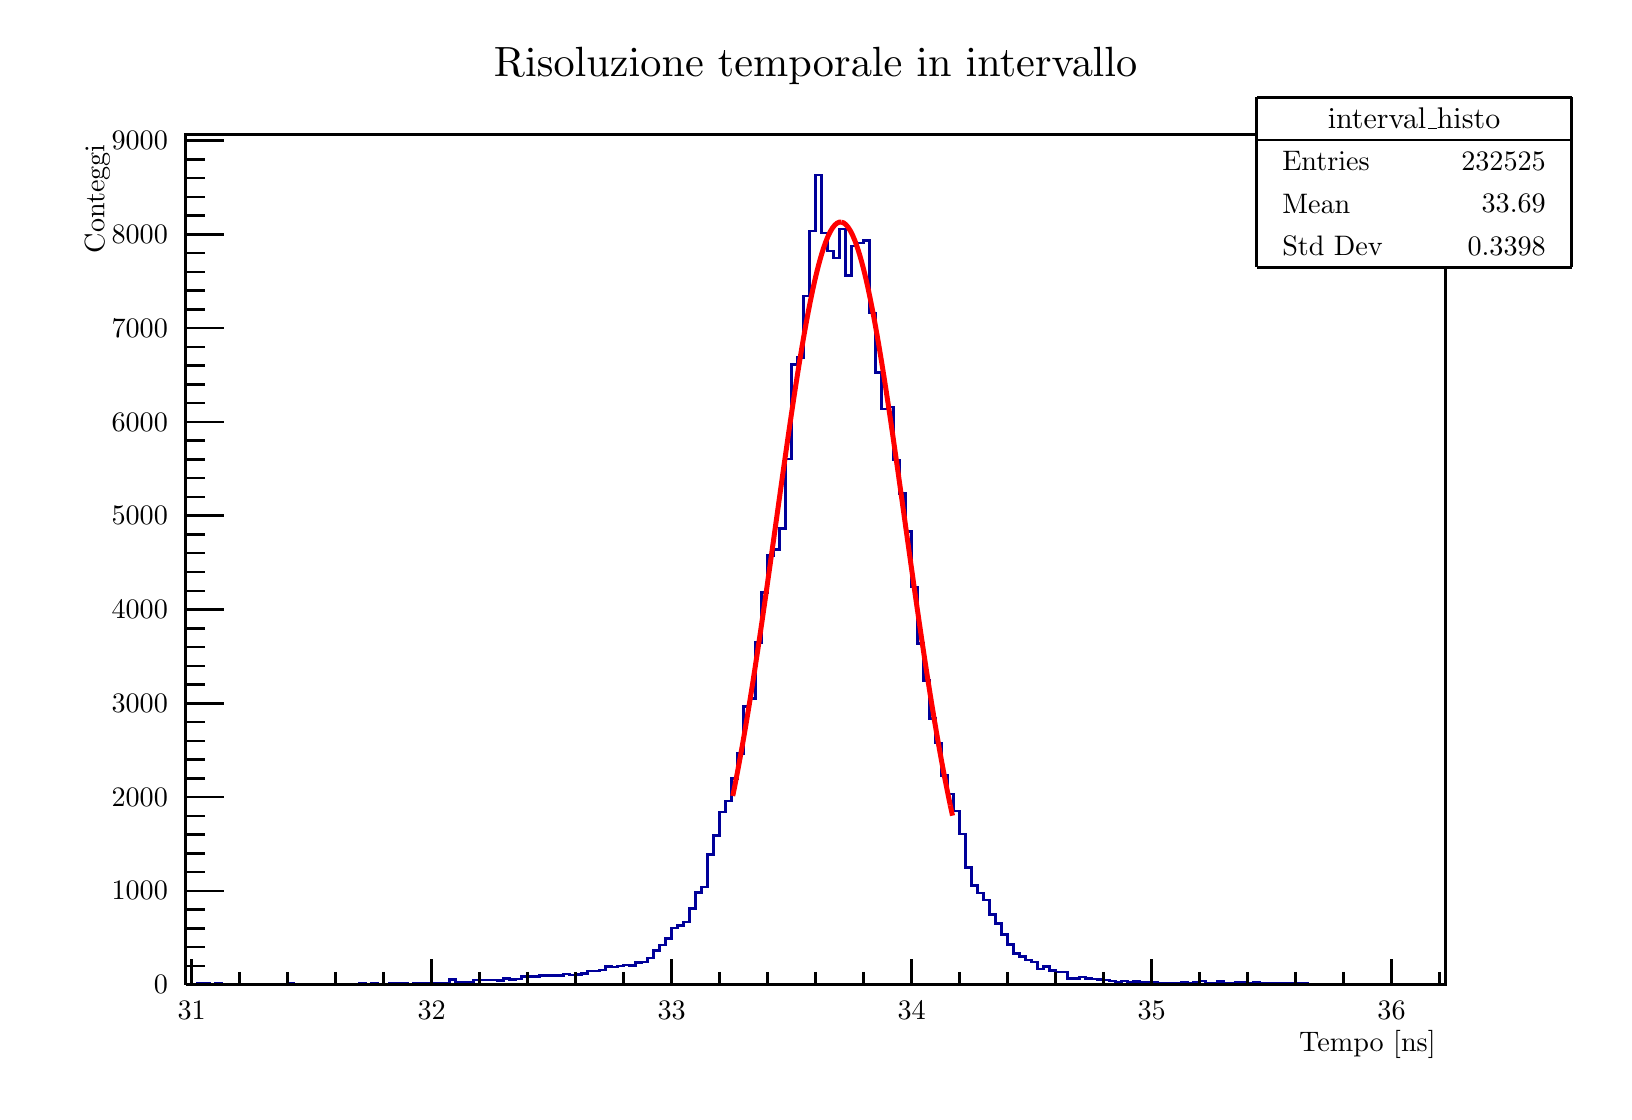
\begin{tikzpicture}
\pgfdeclareplotmark{cross} {
\pgfpathmoveto{\pgfpoint{-0.3\pgfplotmarksize}{\pgfplotmarksize}}
\pgfpathlineto{\pgfpoint{+0.3\pgfplotmarksize}{\pgfplotmarksize}}
\pgfpathlineto{\pgfpoint{+0.3\pgfplotmarksize}{0.3\pgfplotmarksize}}
\pgfpathlineto{\pgfpoint{+1\pgfplotmarksize}{0.3\pgfplotmarksize}}
\pgfpathlineto{\pgfpoint{+1\pgfplotmarksize}{-0.3\pgfplotmarksize}}
\pgfpathlineto{\pgfpoint{+0.3\pgfplotmarksize}{-0.3\pgfplotmarksize}}
\pgfpathlineto{\pgfpoint{+0.3\pgfplotmarksize}{-1.\pgfplotmarksize}}
\pgfpathlineto{\pgfpoint{-0.3\pgfplotmarksize}{-1.\pgfplotmarksize}}
\pgfpathlineto{\pgfpoint{-0.3\pgfplotmarksize}{-0.3\pgfplotmarksize}}
\pgfpathlineto{\pgfpoint{-1.\pgfplotmarksize}{-0.3\pgfplotmarksize}}
\pgfpathlineto{\pgfpoint{-1.\pgfplotmarksize}{0.3\pgfplotmarksize}}
\pgfpathlineto{\pgfpoint{-0.3\pgfplotmarksize}{0.3\pgfplotmarksize}}
\pgfpathclose
\pgfusepathqstroke
}
\pgfdeclareplotmark{cross*} {
\pgfpathmoveto{\pgfpoint{-0.3\pgfplotmarksize}{\pgfplotmarksize}}
\pgfpathlineto{\pgfpoint{+0.3\pgfplotmarksize}{\pgfplotmarksize}}
\pgfpathlineto{\pgfpoint{+0.3\pgfplotmarksize}{0.3\pgfplotmarksize}}
\pgfpathlineto{\pgfpoint{+1\pgfplotmarksize}{0.3\pgfplotmarksize}}
\pgfpathlineto{\pgfpoint{+1\pgfplotmarksize}{-0.3\pgfplotmarksize}}
\pgfpathlineto{\pgfpoint{+0.3\pgfplotmarksize}{-0.3\pgfplotmarksize}}
\pgfpathlineto{\pgfpoint{+0.3\pgfplotmarksize}{-1.\pgfplotmarksize}}
\pgfpathlineto{\pgfpoint{-0.3\pgfplotmarksize}{-1.\pgfplotmarksize}}
\pgfpathlineto{\pgfpoint{-0.3\pgfplotmarksize}{-0.3\pgfplotmarksize}}
\pgfpathlineto{\pgfpoint{-1.\pgfplotmarksize}{-0.3\pgfplotmarksize}}
\pgfpathlineto{\pgfpoint{-1.\pgfplotmarksize}{0.3\pgfplotmarksize}}
\pgfpathlineto{\pgfpoint{-0.3\pgfplotmarksize}{0.3\pgfplotmarksize}}
\pgfpathclose
\pgfusepathqfillstroke
}
\pgfdeclareplotmark{newstar} {
\pgfpathmoveto{\pgfqpoint{0pt}{\pgfplotmarksize}}
\pgfpathlineto{\pgfqpointpolar{44}{0.5\pgfplotmarksize}}
\pgfpathlineto{\pgfqpointpolar{18}{\pgfplotmarksize}}
\pgfpathlineto{\pgfqpointpolar{-20}{0.5\pgfplotmarksize}}
\pgfpathlineto{\pgfqpointpolar{-54}{\pgfplotmarksize}}
\pgfpathlineto{\pgfqpointpolar{-90}{0.5\pgfplotmarksize}}
\pgfpathlineto{\pgfqpointpolar{234}{\pgfplotmarksize}}
\pgfpathlineto{\pgfqpointpolar{198}{0.5\pgfplotmarksize}}
\pgfpathlineto{\pgfqpointpolar{162}{\pgfplotmarksize}}
\pgfpathlineto{\pgfqpointpolar{134}{0.5\pgfplotmarksize}}
\pgfpathclose
\pgfusepathqstroke
}
\pgfdeclareplotmark{newstar*} {
\pgfpathmoveto{\pgfqpoint{0pt}{\pgfplotmarksize}}
\pgfpathlineto{\pgfqpointpolar{44}{0.5\pgfplotmarksize}}
\pgfpathlineto{\pgfqpointpolar{18}{\pgfplotmarksize}}
\pgfpathlineto{\pgfqpointpolar{-20}{0.5\pgfplotmarksize}}
\pgfpathlineto{\pgfqpointpolar{-54}{\pgfplotmarksize}}
\pgfpathlineto{\pgfqpointpolar{-90}{0.5\pgfplotmarksize}}
\pgfpathlineto{\pgfqpointpolar{234}{\pgfplotmarksize}}
\pgfpathlineto{\pgfqpointpolar{198}{0.5\pgfplotmarksize}}
\pgfpathlineto{\pgfqpointpolar{162}{\pgfplotmarksize}}
\pgfpathlineto{\pgfqpointpolar{134}{0.5\pgfplotmarksize}}
\pgfpathclose
\pgfusepathqfillstroke
}
\definecolor{c}{rgb}{1,1,1};
\draw [color=c, fill=c] (0,0) rectangle (20,13.4957);
\draw [color=c, fill=c] (2,1.34957) rectangle (18,12.1461);
\definecolor{c}{rgb}{0,0,0};
\draw [c,line width=0.9] (2,1.34957) -- (2,12.1461) -- (18,12.1461) -- (18,1.34957) -- (2,1.34957);
\definecolor{c}{rgb}{1,1,1};
\draw [color=c, fill=c] (2,1.34957) rectangle (18,12.1461);
\definecolor{c}{rgb}{0,0,0};
\draw [c,line width=0.9] (2,1.34957) -- (2,12.1461) -- (18,12.1461) -- (18,1.34957) -- (2,1.34957);
\definecolor{c}{rgb}{0,0,0.6};
\draw [c,line width=0.9] (2,1.36029) -- (2.07619,1.36029) -- (2.07619,1.35552) -- (2.15238,1.35552) -- (2.15238,1.36148) -- (2.22857,1.36148) -- (2.22857,1.36386) -- (2.30476,1.36386) -- (2.30476,1.35433) -- (2.38095,1.35433) -- (2.38095,1.36386) --
 (2.45714,1.36386) -- (2.45714,1.35552) -- (2.53333,1.35552) -- (2.53333,1.35791) -- (2.60952,1.35791) -- (2.60952,1.35791) -- (2.68571,1.35791) -- (2.68571,1.35672) -- (2.7619,1.35672) -- (2.7619,1.35552) -- (2.8381,1.35552) -- (2.8381,1.35672) --
 (2.91429,1.35672) -- (2.91429,1.35433) -- (2.99048,1.35433) -- (2.99048,1.35672) -- (3.06667,1.35672) -- (3.06667,1.35314) -- (3.14286,1.35314) -- (3.14286,1.35433) -- (3.21905,1.35433) -- (3.21905,1.35552) -- (3.29524,1.35552) -- (3.29524,1.36267)
 -- (3.37143,1.36267) -- (3.37143,1.35314) -- (3.44762,1.35314) -- (3.44762,1.35791) -- (3.52381,1.35791) -- (3.52381,1.35433) -- (3.6,1.35433) -- (3.6,1.35314) -- (3.67619,1.35314) -- (3.67619,1.35076) -- (3.75238,1.35076) -- (3.75238,1.35195) --
 (3.82857,1.35195) -- (3.82857,1.35314) -- (3.90476,1.35314) -- (3.90476,1.35314) -- (3.98095,1.35314) -- (3.98095,1.36029) -- (4.05714,1.36029) -- (4.05714,1.35552) -- (4.13333,1.35552) -- (4.13333,1.35552) -- (4.20952,1.35552) -- (4.20952,1.36148)
 -- (4.28571,1.36148) -- (4.28571,1.35672) -- (4.3619,1.35672) -- (4.3619,1.36386) -- (4.4381,1.36386) -- (4.4381,1.35672) -- (4.51429,1.35672) -- (4.51429,1.36029) -- (4.59048,1.36029) -- (4.59048,1.36267) -- (4.66667,1.36267) -- (4.66667,1.36148)
 -- (4.74286,1.36148) -- (4.74286,1.36386) -- (4.81905,1.36386) -- (4.81905,1.36029) -- (4.89524,1.36029) -- (4.89524,1.37101) -- (4.97143,1.37101) -- (4.97143,1.37101) -- (5.04762,1.37101) -- (5.04762,1.37101) -- (5.12381,1.37101) --
 (5.12381,1.36982) -- (5.2,1.36982) -- (5.2,1.36505) -- (5.27619,1.36505) -- (5.27619,1.36982) -- (5.35238,1.36982) -- (5.35238,1.41388) -- (5.42857,1.41388) -- (5.42857,1.37577) -- (5.50476,1.37577) -- (5.50476,1.3853) -- (5.58095,1.3853) --
 (5.58095,1.37815) -- (5.65714,1.37815) -- (5.65714,1.40673) -- (5.73333,1.40673) -- (5.73333,1.40673) -- (5.80952,1.40673) -- (5.80952,1.40793) -- (5.88571,1.40793) -- (5.88571,1.40912) -- (5.96191,1.40912) -- (5.96191,1.40316) -- (6.0381,1.40316)
 -- (6.0381,1.42936) -- (6.11429,1.42936) -- (6.11429,1.41388) -- (6.19048,1.41388) -- (6.19048,1.41864) -- (6.26667,1.41864) -- (6.26667,1.45556) -- (6.34286,1.45556) -- (6.34286,1.45199) -- (6.41905,1.45199) -- (6.41905,1.4508) -- (6.49524,1.4508)
 -- (6.49524,1.46628) -- (6.57143,1.46628) -- (6.57143,1.4639) -- (6.64762,1.4639) -- (6.64762,1.46628) -- (6.72381,1.46628) -- (6.72381,1.46509) -- (6.8,1.46509) -- (6.8,1.48414) -- (6.87619,1.48414) -- (6.87619,1.46985) -- (6.95238,1.46985) --
 (6.95238,1.48057) -- (7.02857,1.48057) -- (7.02857,1.48891) -- (7.10476,1.48891) -- (7.10476,1.52106) -- (7.18095,1.52106) -- (7.18095,1.52225) -- (7.25714,1.52225) -- (7.25714,1.53416) -- (7.33333,1.53416) -- (7.33333,1.57942) -- (7.40952,1.57942)
 -- (7.40952,1.57108) -- (7.48571,1.57108) -- (7.48571,1.58776) -- (7.5619,1.58776) -- (7.5619,1.59728) -- (7.6381,1.59728) -- (7.6381,1.59371) -- (7.71429,1.59371) -- (7.71429,1.62825) -- (7.79048,1.62825) -- (7.79048,1.63777) -- (7.86667,1.63777)
 -- (7.86667,1.6866) -- (7.94286,1.6866) -- (7.94286,1.78426) -- (8.01905,1.78426) -- (8.01905,1.84976) -- (8.09524,1.84976) -- (8.09524,1.9367) -- (8.17143,1.9367) -- (8.17143,2.0677) -- (8.24762,2.0677) -- (8.24762,2.09985) -- (8.32381,2.09985) --
 (8.32381,2.14511) -- (8.4,2.14511) -- (8.4,2.3166) -- (8.47619,2.3166) -- (8.47619,2.52025) -- (8.55238,2.52025) -- (8.55238,2.58932) -- (8.62857,2.58932) -- (8.62857,3.00138) -- (8.70476,3.00138) -- (8.70476,3.24195) -- (8.78095,3.24195) --
 (8.78095,3.53968) -- (8.85714,3.53968) -- (8.85714,3.6814) -- (8.93333,3.6814) -- (8.93333,3.96841) -- (9.00952,3.96841) -- (9.00952,4.28639) -- (9.08571,4.28639) -- (9.08571,4.87947) -- (9.1619,4.87947) -- (9.1619,4.98189) -- (9.2381,4.98189) --
 (9.2381,5.69644) -- (9.31429,5.69644) -- (9.31429,6.33002) -- (9.39048,6.33002) -- (9.39048,6.80162) -- (9.46667,6.80162) -- (9.46667,6.87308) -- (9.54286,6.87308) -- (9.54286,7.14342) -- (9.61905,7.14342) -- (9.61905,8.02232) -- (9.69524,8.02232)
 -- (9.69524,9.22515) -- (9.77143,9.22515) -- (9.77143,9.31685) -- (9.84762,9.31685) -- (9.84762,10.0933) -- (9.92381,10.0933) -- (9.92381,10.9234) -- (10,10.9234) -- (10,11.632) -- (10.0762,11.632) -- (10.0762,10.8936) -- (10.1524,10.8936) --
 (10.1524,10.6662) -- (10.2286,10.6662) -- (10.2286,10.5804) -- (10.3048,10.5804) -- (10.3048,10.9472) -- (10.381,10.9472) -- (10.381,10.3577) -- (10.4571,10.3577) -- (10.4571,10.7281) -- (10.5333,10.7281) -- (10.5333,10.765) -- (10.6095,10.765) --
 (10.6095,10.7996) -- (10.6857,10.7996) -- (10.6857,9.87659) -- (10.7619,9.87659) -- (10.7619,9.12273) -- (10.8381,9.12273) -- (10.8381,8.65708) -- (10.9143,8.65708) -- (10.9143,8.68685) -- (10.9905,8.68685) -- (10.9905,8.00922) -- (11.0667,8.00922)
 -- (11.0667,7.58763) -- (11.1429,7.58763) -- (11.1429,7.1065) -- (11.219,7.1065) -- (11.219,6.3979) -- (11.2952,6.3979) -- (11.2952,5.67858) -- (11.3714,5.67858) -- (11.3714,5.21293) -- (11.4476,5.21293) -- (11.4476,4.7306) -- (11.5238,4.7306) --
 (11.5238,4.41977) -- (11.6,4.41977) -- (11.6,4.00533) -- (11.6762,4.00533) -- (11.6762,3.77191) -- (11.7524,3.77191) -- (11.7524,3.55635) -- (11.8286,3.55635) -- (11.8286,3.261) -- (11.9048,3.261) -- (11.9048,2.83823) -- (11.981,2.83823) --
 (11.981,2.60957) -- (12.0571,2.60957) -- (12.0571,2.51072) -- (12.1333,2.51072) -- (12.1333,2.42378) -- (12.2095,2.42378) -- (12.2095,2.23919) -- (12.2857,2.23919) -- (12.2857,2.12843) -- (12.3619,2.12843) -- (12.3619,1.98552) -- (12.4381,1.98552)
 -- (12.4381,1.85929) -- (12.5143,1.85929) -- (12.5143,1.74496) -- (12.5905,1.74496) -- (12.5905,1.70804) -- (12.6667,1.70804) -- (12.6667,1.66278) -- (12.7429,1.66278) -- (12.7429,1.63658) -- (12.819,1.63658) -- (12.819,1.55084) -- (12.8952,1.55084)
 -- (12.8952,1.57823) -- (12.9714,1.57823) -- (12.9714,1.52821) -- (13.0476,1.52821) -- (13.0476,1.51273) -- (13.1238,1.51273) -- (13.1238,1.51273) -- (13.2,1.51273) -- (13.2,1.42936) -- (13.2762,1.42936) -- (13.2762,1.4246) -- (13.3524,1.4246) --
 (13.3524,1.44484) -- (13.4286,1.44484) -- (13.4286,1.42936) -- (13.5048,1.42936) -- (13.5048,1.42222) -- (13.581,1.42222) -- (13.581,1.41626) -- (13.6571,1.41626) -- (13.6571,1.40793) -- (13.7333,1.40793) -- (13.7333,1.39244) -- (13.8095,1.39244) --
 (13.8095,1.38411) -- (13.8857,1.38411) -- (13.8857,1.39721) -- (13.9619,1.39721) -- (13.9619,1.3853) -- (14.0381,1.3853) -- (14.0381,1.38768) -- (14.1143,1.38768) -- (14.1143,1.37934) -- (14.1905,1.37934) -- (14.1905,1.37696) -- (14.2667,1.37696) --
 (14.2667,1.38411) -- (14.3429,1.38411) -- (14.3429,1.3722) -- (14.419,1.3722) -- (14.419,1.37101) -- (14.4952,1.37101) -- (14.4952,1.36863) -- (14.5714,1.36863) -- (14.5714,1.36982) -- (14.6476,1.36982) -- (14.6476,1.37339) -- (14.7238,1.37339) --
 (14.7238,1.3722) -- (14.8,1.3722) -- (14.8,1.37458) -- (14.8762,1.37458) -- (14.8762,1.39483) -- (14.9524,1.39483) -- (14.9524,1.37101) -- (15.0286,1.37101) -- (15.0286,1.36743) -- (15.1048,1.36743) -- (15.1048,1.38649) -- (15.181,1.38649) --
 (15.181,1.37101) -- (15.2571,1.37101) -- (15.2571,1.36863) -- (15.3333,1.36863) -- (15.3333,1.37339) -- (15.4095,1.37339) -- (15.4095,1.37458) -- (15.4857,1.37458) -- (15.4857,1.36743) -- (15.5619,1.36743) -- (15.5619,1.37815) -- (15.6381,1.37815)
 -- (15.6381,1.36982) -- (15.7143,1.36982) -- (15.7143,1.36505) -- (15.7905,1.36505) -- (15.7905,1.37101) -- (15.8667,1.37101) -- (15.8667,1.36863) -- (15.9429,1.36863) -- (15.9429,1.37101) -- (16.019,1.37101) -- (16.019,1.36386) -- (16.0952,1.36386)
 -- (16.0952,1.36505) -- (16.1714,1.36505) -- (16.1714,1.36624) -- (16.2476,1.36624) -- (16.2476,1.36029) -- (16.3238,1.36029) -- (16.3238,1.35791) -- (16.4,1.35791) -- (16.4,1.35433) -- (16.4762,1.35433) -- (16.4762,1.36029) -- (16.5524,1.36029) --
 (16.5524,1.35791) -- (16.6286,1.35791) -- (16.6286,1.35076) -- (16.7048,1.35076) -- (16.7048,1.35076) -- (16.781,1.35076) -- (16.781,1.35433) -- (16.8571,1.35433) -- (16.8571,1.35195) -- (16.9333,1.35195) -- (16.9333,1.35195) -- (17.0095,1.35195) --
 (17.0095,1.34957) -- (17.0857,1.34957) -- (17.0857,1.35314) -- (17.1619,1.35314) -- (17.1619,1.34957) -- (17.2381,1.34957) -- (17.2381,1.34957) -- (17.3143,1.34957) -- (17.3143,1.34957) -- (17.3905,1.34957) -- (17.3905,1.34957) -- (17.4667,1.34957)
 -- (17.4667,1.34957) -- (17.5429,1.34957) -- (17.5429,1.35195) -- (17.619,1.35195) -- (17.619,1.34957) -- (17.6952,1.34957) -- (17.6952,1.35076) -- (17.7714,1.35076) -- (17.7714,1.35314) -- (17.8476,1.35314) -- (17.8476,1.35076) -- (17.9238,1.35076)
 -- (17.9238,1.35076) -- (18,1.35076);
\definecolor{c}{rgb}{1,1,1};
\draw [color=c, fill=c] (15.6,10.4592) rectangle (19.6,12.6185);
\definecolor{c}{rgb}{0,0,0};
\draw [c,line width=0.9] (15.6,10.4592) -- (19.6,10.4592);
\draw [c,line width=0.9] (19.6,10.4592) -- (19.6,12.6185);
\draw [c,line width=0.9] (19.6,12.6185) -- (15.6,12.6185);
\draw [c,line width=0.9] (15.6,12.6185) -- (15.6,10.4592);
\draw (17.6,12.3486) node[scale=1.08185, color=c, rotate=0]{interval\_histo};
\draw [c,line width=0.9] (15.6,12.0787) -- (19.6,12.0787);
\draw [anchor= west] (15.8,11.8087) node[scale=1.01821, color=c, rotate=0]{Entries };
\draw [anchor= east] (19.4,11.8087) node[scale=1.01821, color=c, rotate=0]{ 232525};
\draw [anchor= west] (15.8,11.2689) node[scale=1.01821, color=c, rotate=0]{Mean  };
\draw [anchor= east] (19.4,11.2689) node[scale=1.01821, color=c, rotate=0]{  33.69};
\draw [anchor= west] (15.8,10.7291) node[scale=1.01821, color=c, rotate=0]{Std Dev   };
\draw [anchor= east] (19.4,10.7291) node[scale=1.01821, color=c, rotate=0]{ 0.3398};
\definecolor{c}{rgb}{1,0,0};
\draw [c,line width=1.8] (8.94743,3.74517) -- (8.97562,3.88553) -- (9.00381,4.03094) -- (9.032,4.18133) -- (9.06019,4.33662) -- (9.08838,4.49669) -- (9.11657,4.66141) -- (9.14476,4.83063) -- (9.17295,5.00415) -- (9.20114,5.18179) -- (9.22933,5.3633)
 -- (9.25752,5.54844) -- (9.28571,5.73691) -- (9.3139,5.92841) -- (9.3421,6.12261) -- (9.37029,6.31916) -- (9.39848,6.51768) -- (9.42667,6.71776) -- (9.45486,6.91899) -- (9.48305,7.12091) -- (9.51124,7.32308) -- (9.53943,7.52501) -- (9.56762,7.72621)
 -- (9.59581,7.92616) -- (9.624,8.12435) -- (9.65219,8.32026) -- (9.68038,8.51333) -- (9.70857,8.70304) -- (9.73676,8.88883) -- (9.76495,9.07016) -- (9.79314,9.24649) -- (9.82133,9.41729) -- (9.84952,9.58202) -- (9.87771,9.74017) -- (9.9059,9.89123)
 -- (9.9341,10.0347) -- (9.96229,10.1702) -- (9.99048,10.2971) -- (10.0187,10.4151) -- (10.0469,10.5238) -- (10.075,10.6228) -- (10.1032,10.7118) -- (10.1314,10.7905) -- (10.1596,10.8585) -- (10.1878,10.9157) -- (10.216,10.9618) -- (10.2442,10.9968)
 -- (10.2724,11.0203) -- (10.3006,11.0325) -- (10.3288,11.0332);
\draw [c,line width=1.8] (10.3288,11.0332) -- (10.357,11.0224) -- (10.3851,11.0002) -- (10.4133,10.9667) -- (10.4415,10.9219) -- (10.4697,10.8661) -- (10.4979,10.7993) -- (10.5261,10.722) -- (10.5543,10.6342) -- (10.5825,10.5364) -- (10.6107,10.4289)
 -- (10.6389,10.312) -- (10.667,10.1861) -- (10.6952,10.0517) -- (10.7234,9.90913) -- (10.7516,9.75897) -- (10.7798,9.60166) -- (10.808,9.4377) -- (10.8362,9.26762) -- (10.8644,9.09193) -- (10.8926,8.91118) -- (10.9208,8.7259) -- (10.949,8.53664) --
 (10.9771,8.34395) -- (11.0053,8.14836) -- (11.0335,7.95042) -- (11.0617,7.75065) -- (11.0899,7.54958) -- (11.1181,7.34772) -- (11.1463,7.14555) -- (11.1745,6.94357) -- (11.2027,6.74224) -- (11.2309,6.54199) -- (11.259,6.34326) -- (11.2872,6.14645)
 -- (11.3154,5.95194) -- (11.3436,5.76009) -- (11.3718,5.57124) -- (11.4,5.38568) -- (11.4282,5.20371) -- (11.4564,5.02559) -- (11.4846,4.85155) -- (11.5128,4.6818) -- (11.541,4.51652) -- (11.5691,4.35588) -- (11.5973,4.2) -- (11.6255,4.04901) --
 (11.6537,3.90299) -- (11.6819,3.76201) -- (11.7101,3.62611);
\draw [c,line width=1.8] (11.7101,3.62611) -- (11.7383,3.49533);
\definecolor{c}{rgb}{0,0,0};
\draw [c,line width=0.9] (2,1.34957) -- (18,1.34957);
\draw [anchor= east] (18,0.593811) node[scale=1.01821, color=c, rotate=0]{Tempo [ns]};
\draw [c,line width=0.9] (2.07619,1.67347) -- (2.07619,1.34957);
\draw [c,line width=0.9] (2.68571,1.51152) -- (2.68571,1.34957);
\draw [c,line width=0.9] (3.29524,1.51152) -- (3.29524,1.34957);
\draw [c,line width=0.9] (3.90476,1.51152) -- (3.90476,1.34957);
\draw [c,line width=0.9] (4.51429,1.51152) -- (4.51429,1.34957);
\draw [c,line width=0.9] (5.12381,1.67347) -- (5.12381,1.34957);
\draw [c,line width=0.9] (5.73333,1.51152) -- (5.73333,1.34957);
\draw [c,line width=0.9] (6.34286,1.51152) -- (6.34286,1.34957);
\draw [c,line width=0.9] (6.95238,1.51152) -- (6.95238,1.34957);
\draw [c,line width=0.9] (7.5619,1.51152) -- (7.5619,1.34957);
\draw [c,line width=0.9] (8.17143,1.67347) -- (8.17143,1.34957);
\draw [c,line width=0.9] (8.78095,1.51152) -- (8.78095,1.34957);
\draw [c,line width=0.9] (9.39048,1.51152) -- (9.39048,1.34957);
\draw [c,line width=0.9] (10,1.51152) -- (10,1.34957);
\draw [c,line width=0.9] (10.6095,1.51152) -- (10.6095,1.34957);
\draw [c,line width=0.9] (11.219,1.67347) -- (11.219,1.34957);
\draw [c,line width=0.9] (11.8286,1.51152) -- (11.8286,1.34957);
\draw [c,line width=0.9] (12.4381,1.51152) -- (12.4381,1.34957);
\draw [c,line width=0.9] (13.0476,1.51152) -- (13.0476,1.34957);
\draw [c,line width=0.9] (13.6571,1.51152) -- (13.6571,1.34957);
\draw [c,line width=0.9] (14.2667,1.67347) -- (14.2667,1.34957);
\draw [c,line width=0.9] (14.8762,1.51152) -- (14.8762,1.34957);
\draw [c,line width=0.9] (15.4857,1.51152) -- (15.4857,1.34957);
\draw [c,line width=0.9] (16.0952,1.51152) -- (16.0952,1.34957);
\draw [c,line width=0.9] (16.7048,1.51152) -- (16.7048,1.34957);
\draw [c,line width=0.9] (17.3143,1.67347) -- (17.3143,1.34957);
\draw [c,line width=0.9] (2.07619,1.67347) -- (2.07619,1.34957);
\draw [c,line width=0.9] (17.3143,1.67347) -- (17.3143,1.34957);
\draw [c,line width=0.9] (17.9238,1.51152) -- (17.9238,1.34957);
\draw [anchor=base] (2.07619,0.904212) node[scale=1.01821, color=c, rotate=0]{31};
\draw [anchor=base] (5.12381,0.904212) node[scale=1.01821, color=c, rotate=0]{32};
\draw [anchor=base] (8.17143,0.904212) node[scale=1.01821, color=c, rotate=0]{33};
\draw [anchor=base] (11.219,0.904212) node[scale=1.01821, color=c, rotate=0]{34};
\draw [anchor=base] (14.2667,0.904212) node[scale=1.01821, color=c, rotate=0]{35};
\draw [anchor=base] (17.3143,0.904212) node[scale=1.01821, color=c, rotate=0]{36};
\draw [c,line width=0.9] (2,1.34957) -- (2,12.1461);
\draw [anchor= east] (0.88,12.1461) node[scale=1.01821, color=c, rotate=90]{Conteggi};
\draw [c,line width=0.9] (2.48,1.34957) -- (2,1.34957);
\draw [c,line width=0.9] (2.24,1.58776) -- (2,1.58776);
\draw [c,line width=0.9] (2.24,1.82594) -- (2,1.82594);
\draw [c,line width=0.9] (2.24,2.06412) -- (2,2.06412);
\draw [c,line width=0.9] (2.24,2.30231) -- (2,2.30231);
\draw [c,line width=0.9] (2.48,2.54049) -- (2,2.54049);
\draw [c,line width=0.9] (2.24,2.77868) -- (2,2.77868);
\draw [c,line width=0.9] (2.24,3.01686) -- (2,3.01686);
\draw [c,line width=0.9] (2.24,3.25505) -- (2,3.25505);
\draw [c,line width=0.9] (2.24,3.49323) -- (2,3.49323);
\draw [c,line width=0.9] (2.48,3.73142) -- (2,3.73142);
\draw [c,line width=0.9] (2.24,3.9696) -- (2,3.9696);
\draw [c,line width=0.9] (2.24,4.20779) -- (2,4.20779);
\draw [c,line width=0.9] (2.24,4.44597) -- (2,4.44597);
\draw [c,line width=0.9] (2.24,4.68416) -- (2,4.68416);
\draw [c,line width=0.9] (2.48,4.92234) -- (2,4.92234);
\draw [c,line width=0.9] (2.24,5.16053) -- (2,5.16053);
\draw [c,line width=0.9] (2.24,5.39871) -- (2,5.39871);
\draw [c,line width=0.9] (2.24,5.6369) -- (2,5.6369);
\draw [c,line width=0.9] (2.24,5.87508) -- (2,5.87508);
\draw [c,line width=0.9] (2.48,6.11327) -- (2,6.11327);
\draw [c,line width=0.9] (2.24,6.35145) -- (2,6.35145);
\draw [c,line width=0.9] (2.24,6.58964) -- (2,6.58964);
\draw [c,line width=0.9] (2.24,6.82782) -- (2,6.82782);
\draw [c,line width=0.9] (2.24,7.06601) -- (2,7.06601);
\draw [c,line width=0.9] (2.48,7.30419) -- (2,7.30419);
\draw [c,line width=0.9] (2.24,7.54238) -- (2,7.54238);
\draw [c,line width=0.9] (2.24,7.78056) -- (2,7.78056);
\draw [c,line width=0.9] (2.24,8.01875) -- (2,8.01875);
\draw [c,line width=0.9] (2.24,8.25693) -- (2,8.25693);
\draw [c,line width=0.9] (2.48,8.49512) -- (2,8.49512);
\draw [c,line width=0.9] (2.24,8.7333) -- (2,8.7333);
\draw [c,line width=0.9] (2.24,8.97149) -- (2,8.97149);
\draw [c,line width=0.9] (2.24,9.20967) -- (2,9.20967);
\draw [c,line width=0.9] (2.24,9.44785) -- (2,9.44785);
\draw [c,line width=0.9] (2.48,9.68604) -- (2,9.68604);
\draw [c,line width=0.9] (2.24,9.92422) -- (2,9.92422);
\draw [c,line width=0.9] (2.24,10.1624) -- (2,10.1624);
\draw [c,line width=0.9] (2.24,10.4006) -- (2,10.4006);
\draw [c,line width=0.9] (2.24,10.6388) -- (2,10.6388);
\draw [c,line width=0.9] (2.48,10.877) -- (2,10.877);
\draw [c,line width=0.9] (2.24,11.1151) -- (2,11.1151);
\draw [c,line width=0.9] (2.24,11.3533) -- (2,11.3533);
\draw [c,line width=0.9] (2.24,11.5915) -- (2,11.5915);
\draw [c,line width=0.9] (2.24,11.8297) -- (2,11.8297);
\draw [c,line width=0.9] (2.48,12.0679) -- (2,12.0679);
\draw [c,line width=0.9] (2.48,12.0679) -- (2,12.0679);
\draw [anchor= east] (1.9,1.34957) node[scale=1.01821, color=c, rotate=0]{0};
\draw [anchor= east] (1.9,2.54049) node[scale=1.01821, color=c, rotate=0]{1000};
\draw [anchor= east] (1.9,3.73142) node[scale=1.01821, color=c, rotate=0]{2000};
\draw [anchor= east] (1.9,4.92234) node[scale=1.01821, color=c, rotate=0]{3000};
\draw [anchor= east] (1.9,6.11327) node[scale=1.01821, color=c, rotate=0]{4000};
\draw [anchor= east] (1.9,7.30419) node[scale=1.01821, color=c, rotate=0]{5000};
\draw [anchor= east] (1.9,8.49512) node[scale=1.01821, color=c, rotate=0]{6000};
\draw [anchor= east] (1.9,9.68604) node[scale=1.01821, color=c, rotate=0]{7000};
\draw [anchor= east] (1.9,10.877) node[scale=1.01821, color=c, rotate=0]{8000};
\draw [anchor= east] (1.9,12.0679) node[scale=1.01821, color=c, rotate=0]{9000};
\definecolor{c}{rgb}{1,1,1};
\draw [color=c, fill=c] (15.6,10.4592) rectangle (19.6,12.6185);
\definecolor{c}{rgb}{0,0,0};
\draw [c,line width=0.9] (15.6,10.4592) -- (19.6,10.4592);
\draw [c,line width=0.9] (19.6,10.4592) -- (19.6,12.6185);
\draw [c,line width=0.9] (19.6,12.6185) -- (15.6,12.6185);
\draw [c,line width=0.9] (15.6,12.6185) -- (15.6,10.4592);
\draw (17.6,12.3486) node[scale=1.08185, color=c, rotate=0]{interval\_histo};
\draw [c,line width=0.9] (15.6,12.0787) -- (19.6,12.0787);
\draw [anchor= west] (15.8,11.8087) node[scale=1.01821, color=c, rotate=0]{Entries };
\draw [anchor= east] (19.4,11.8087) node[scale=1.01821, color=c, rotate=0]{ 232525};
\draw [anchor= west] (15.8,11.2689) node[scale=1.01821, color=c, rotate=0]{Mean  };
\draw [anchor= east] (19.4,11.2689) node[scale=1.01821, color=c, rotate=0]{  33.69};
\draw [anchor= west] (15.8,10.7291) node[scale=1.01821, color=c, rotate=0]{Std Dev   };
\draw [anchor= east] (19.4,10.7291) node[scale=1.01821, color=c, rotate=0]{ 0.3398};
\draw (10,13.0156) node[scale=1.52731, color=c, rotate=0]{Risoluzione temporale in intervallo};
\end{tikzpicture}

%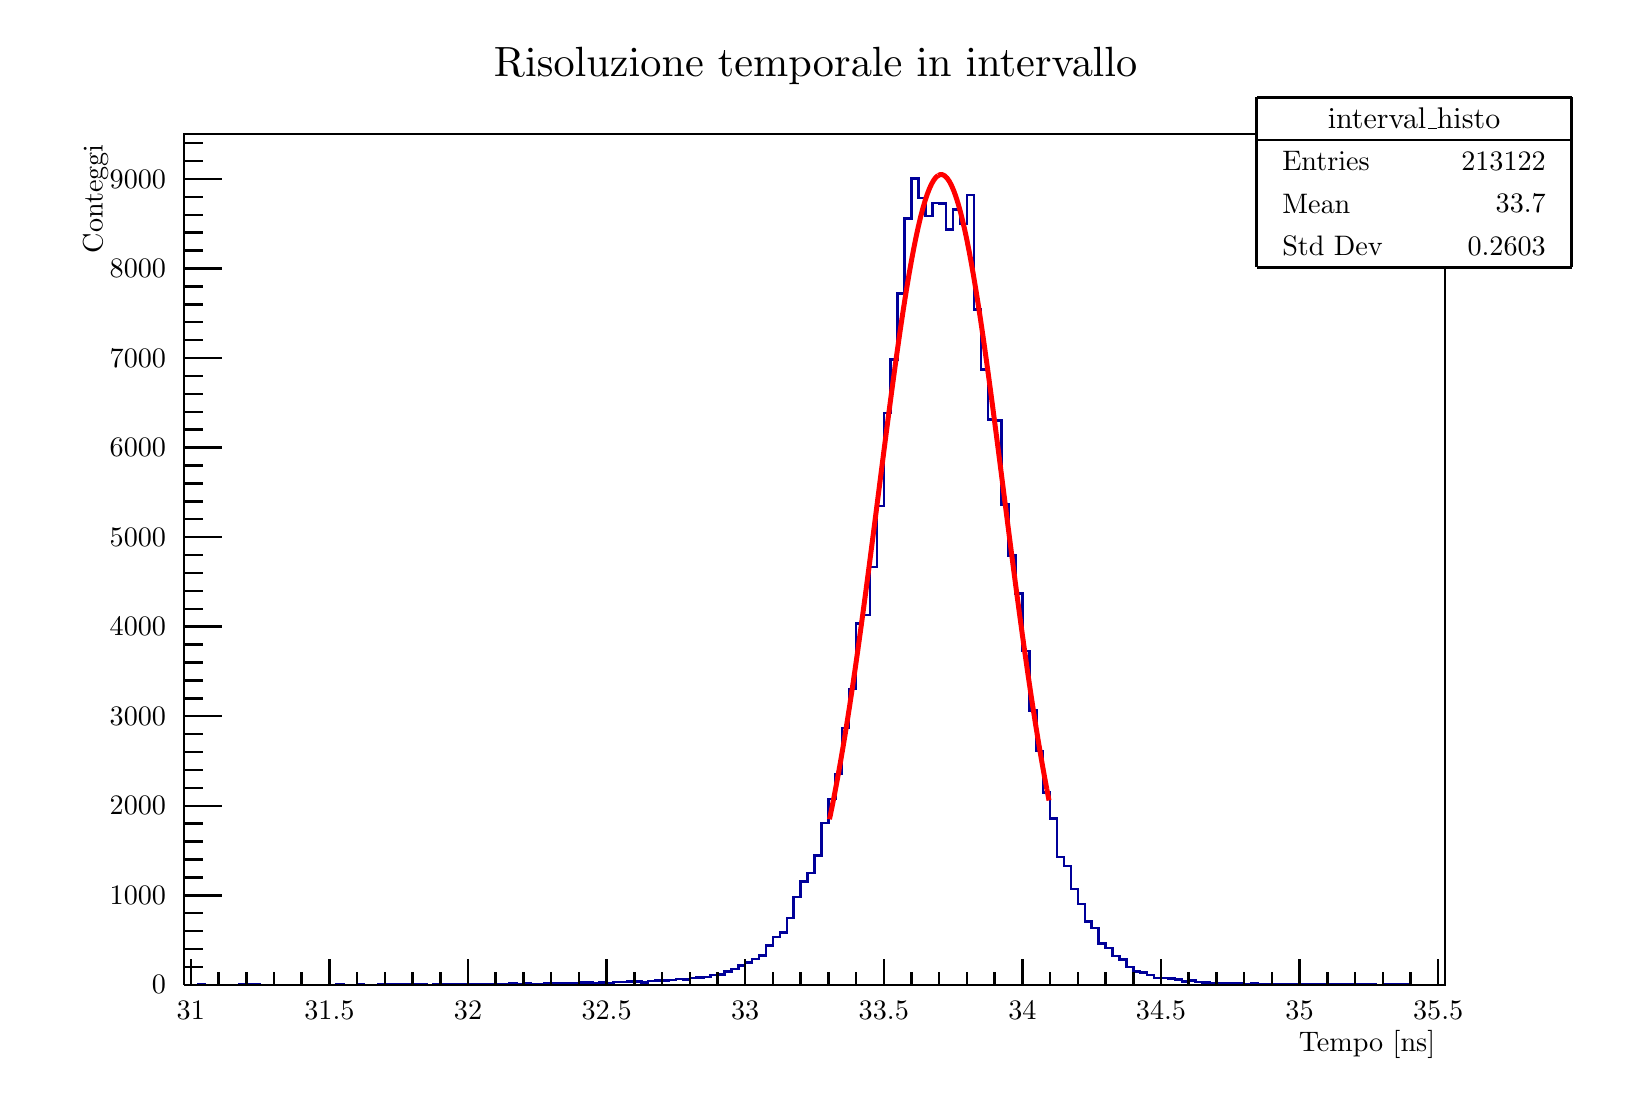
\begin{tikzpicture}
\pgfdeclareplotmark{cross} {
\pgfpathmoveto{\pgfpoint{-0.3\pgfplotmarksize}{\pgfplotmarksize}}
\pgfpathlineto{\pgfpoint{+0.3\pgfplotmarksize}{\pgfplotmarksize}}
\pgfpathlineto{\pgfpoint{+0.3\pgfplotmarksize}{0.3\pgfplotmarksize}}
\pgfpathlineto{\pgfpoint{+1\pgfplotmarksize}{0.3\pgfplotmarksize}}
\pgfpathlineto{\pgfpoint{+1\pgfplotmarksize}{-0.3\pgfplotmarksize}}
\pgfpathlineto{\pgfpoint{+0.3\pgfplotmarksize}{-0.3\pgfplotmarksize}}
\pgfpathlineto{\pgfpoint{+0.3\pgfplotmarksize}{-1.\pgfplotmarksize}}
\pgfpathlineto{\pgfpoint{-0.3\pgfplotmarksize}{-1.\pgfplotmarksize}}
\pgfpathlineto{\pgfpoint{-0.3\pgfplotmarksize}{-0.3\pgfplotmarksize}}
\pgfpathlineto{\pgfpoint{-1.\pgfplotmarksize}{-0.3\pgfplotmarksize}}
\pgfpathlineto{\pgfpoint{-1.\pgfplotmarksize}{0.3\pgfplotmarksize}}
\pgfpathlineto{\pgfpoint{-0.3\pgfplotmarksize}{0.3\pgfplotmarksize}}
\pgfpathclose
\pgfusepathqstroke
}
\pgfdeclareplotmark{cross*} {
\pgfpathmoveto{\pgfpoint{-0.3\pgfplotmarksize}{\pgfplotmarksize}}
\pgfpathlineto{\pgfpoint{+0.3\pgfplotmarksize}{\pgfplotmarksize}}
\pgfpathlineto{\pgfpoint{+0.3\pgfplotmarksize}{0.3\pgfplotmarksize}}
\pgfpathlineto{\pgfpoint{+1\pgfplotmarksize}{0.3\pgfplotmarksize}}
\pgfpathlineto{\pgfpoint{+1\pgfplotmarksize}{-0.3\pgfplotmarksize}}
\pgfpathlineto{\pgfpoint{+0.3\pgfplotmarksize}{-0.3\pgfplotmarksize}}
\pgfpathlineto{\pgfpoint{+0.3\pgfplotmarksize}{-1.\pgfplotmarksize}}
\pgfpathlineto{\pgfpoint{-0.3\pgfplotmarksize}{-1.\pgfplotmarksize}}
\pgfpathlineto{\pgfpoint{-0.3\pgfplotmarksize}{-0.3\pgfplotmarksize}}
\pgfpathlineto{\pgfpoint{-1.\pgfplotmarksize}{-0.3\pgfplotmarksize}}
\pgfpathlineto{\pgfpoint{-1.\pgfplotmarksize}{0.3\pgfplotmarksize}}
\pgfpathlineto{\pgfpoint{-0.3\pgfplotmarksize}{0.3\pgfplotmarksize}}
\pgfpathclose
\pgfusepathqfillstroke
}
\pgfdeclareplotmark{newstar} {
\pgfpathmoveto{\pgfqpoint{0pt}{\pgfplotmarksize}}
\pgfpathlineto{\pgfqpointpolar{44}{0.5\pgfplotmarksize}}
\pgfpathlineto{\pgfqpointpolar{18}{\pgfplotmarksize}}
\pgfpathlineto{\pgfqpointpolar{-20}{0.5\pgfplotmarksize}}
\pgfpathlineto{\pgfqpointpolar{-54}{\pgfplotmarksize}}
\pgfpathlineto{\pgfqpointpolar{-90}{0.5\pgfplotmarksize}}
\pgfpathlineto{\pgfqpointpolar{234}{\pgfplotmarksize}}
\pgfpathlineto{\pgfqpointpolar{198}{0.5\pgfplotmarksize}}
\pgfpathlineto{\pgfqpointpolar{162}{\pgfplotmarksize}}
\pgfpathlineto{\pgfqpointpolar{134}{0.5\pgfplotmarksize}}
\pgfpathclose
\pgfusepathqstroke
}
\pgfdeclareplotmark{newstar*} {
\pgfpathmoveto{\pgfqpoint{0pt}{\pgfplotmarksize}}
\pgfpathlineto{\pgfqpointpolar{44}{0.5\pgfplotmarksize}}
\pgfpathlineto{\pgfqpointpolar{18}{\pgfplotmarksize}}
\pgfpathlineto{\pgfqpointpolar{-20}{0.5\pgfplotmarksize}}
\pgfpathlineto{\pgfqpointpolar{-54}{\pgfplotmarksize}}
\pgfpathlineto{\pgfqpointpolar{-90}{0.5\pgfplotmarksize}}
\pgfpathlineto{\pgfqpointpolar{234}{\pgfplotmarksize}}
\pgfpathlineto{\pgfqpointpolar{198}{0.5\pgfplotmarksize}}
\pgfpathlineto{\pgfqpointpolar{162}{\pgfplotmarksize}}
\pgfpathlineto{\pgfqpointpolar{134}{0.5\pgfplotmarksize}}
\pgfpathclose
\pgfusepathqfillstroke
}
\definecolor{c}{rgb}{1,1,1};
\draw [color=c, fill=c] (0,0) rectangle (20,13.4957);
\draw [color=c, fill=c] (1.97708,1.3467) rectangle (17.9943,12.149);
\definecolor{c}{rgb}{0,0,0};
\draw [c,line width=0.9] (1.97708,1.3467) -- (1.97708,12.149) -- (17.9943,12.149) -- (17.9943,1.3467) -- (1.97708,1.3467);
\definecolor{c}{rgb}{1,1,1};
\draw [color=c, fill=c] (1.97708,1.3467) rectangle (17.9943,12.149);
\definecolor{c}{rgb}{0,0,0};
\draw [c,line width=0.9] (1.97708,1.3467) -- (1.97708,12.149) -- (17.9943,12.149) -- (17.9943,1.3467) -- (1.97708,1.3467);
\definecolor{c}{rgb}{0,0,0.6};
\draw [c,line width=0.9] (1.97708,1.3467) -- (2.06508,1.3467) -- (2.06508,1.3467) -- (2.15309,1.3467) -- (2.15309,1.34898) -- (2.2411,1.34898) -- (2.2411,1.3467) -- (2.3291,1.3467) -- (2.3291,1.3467) -- (2.41711,1.3467) -- (2.41711,1.3467) --
 (2.50512,1.3467) -- (2.50512,1.34784) -- (2.59312,1.34784) -- (2.59312,1.3467) -- (2.68113,1.3467) -- (2.68113,1.34898) -- (2.76914,1.34898) -- (2.76914,1.34898) -- (2.85714,1.34898) -- (2.85714,1.34898) -- (2.94515,1.34898) -- (2.94515,1.34784) --
 (3.03316,1.34784) -- (3.03316,1.3467) -- (3.12116,1.3467) -- (3.12116,1.34784) -- (3.20917,1.34784) -- (3.20917,1.34784) -- (3.29718,1.34784) -- (3.29718,1.3467) -- (3.38518,1.3467) -- (3.38518,1.3467) -- (3.47319,1.3467) -- (3.47319,1.34784) --
 (3.5612,1.34784) -- (3.5612,1.3467) -- (3.6492,1.3467) -- (3.6492,1.34784) -- (3.73721,1.34784) -- (3.73721,1.3467) -- (3.82521,1.3467) -- (3.82521,1.34784) -- (3.91322,1.34784) -- (3.91322,1.34898) -- (4.00123,1.34898) -- (4.00123,1.34784) --
 (4.08923,1.34784) -- (4.08923,1.3467) -- (4.17724,1.3467) -- (4.17724,1.34898) -- (4.26525,1.34898) -- (4.26525,1.3467) -- (4.35325,1.3467) -- (4.35325,1.34784) -- (4.44126,1.34784) -- (4.44126,1.35012) -- (4.52927,1.35012) -- (4.52927,1.35012) --
 (4.61727,1.35012) -- (4.61727,1.34898) -- (4.70528,1.34898) -- (4.70528,1.34898) -- (4.79329,1.34898) -- (4.79329,1.34898) -- (4.88129,1.34898) -- (4.88129,1.35125) -- (4.9693,1.35125) -- (4.9693,1.34898) -- (5.05731,1.34898) -- (5.05731,1.3467) --
 (5.14531,1.3467) -- (5.14531,1.35125) -- (5.23332,1.35125) -- (5.23332,1.35012) -- (5.32133,1.35012) -- (5.32133,1.35125) -- (5.40933,1.35125) -- (5.40933,1.34898) -- (5.49734,1.34898) -- (5.49734,1.35353) -- (5.58535,1.35353) -- (5.58535,1.35125)
 -- (5.67335,1.35125) -- (5.67335,1.35239) -- (5.76136,1.35239) -- (5.76136,1.35808) -- (5.84937,1.35808) -- (5.84937,1.3558) -- (5.93737,1.3558) -- (5.93737,1.35353) -- (6.02538,1.35353) -- (6.02538,1.35239) -- (6.11339,1.35239) -- (6.11339,1.36149)
 -- (6.20139,1.36149) -- (6.20139,1.35694) -- (6.2894,1.35694) -- (6.2894,1.36376) -- (6.3774,1.36376) -- (6.3774,1.35467) -- (6.46541,1.35467) -- (6.46541,1.35694) -- (6.55342,1.35694) -- (6.55342,1.36831) -- (6.64142,1.36831) -- (6.64142,1.36945)
 -- (6.72943,1.36945) -- (6.72943,1.36945) -- (6.81744,1.36945) -- (6.81744,1.36717) -- (6.90544,1.36717) -- (6.90544,1.37286) -- (6.99345,1.37286) -- (6.99345,1.37855) -- (7.08146,1.37855) -- (7.08146,1.37741) -- (7.16946,1.37741) --
 (7.16946,1.37059) -- (7.25747,1.37059) -- (7.25747,1.37741) -- (7.34548,1.37741) -- (7.34548,1.36831) -- (7.43348,1.36831) -- (7.43348,1.38423) -- (7.52149,1.38423) -- (7.52149,1.38196) -- (7.6095,1.38196) -- (7.6095,1.38992) -- (7.6975,1.38992) --
 (7.6975,1.39219) -- (7.78551,1.39219) -- (7.78551,1.37627) -- (7.87352,1.37627) -- (7.87352,1.39447) -- (7.96152,1.39447) -- (7.96152,1.40015) -- (8.04953,1.40015) -- (8.04953,1.40356) -- (8.13754,1.40356) -- (8.13754,1.40811) -- (8.22554,1.40811)
 -- (8.22554,1.4229) -- (8.31355,1.4229) -- (8.31355,1.41153) -- (8.40156,1.41153) -- (8.40156,1.43199) -- (8.48956,1.43199) -- (8.48956,1.43995) -- (8.57757,1.43995) -- (8.57757,1.4445) -- (8.66558,1.4445) -- (8.66558,1.47066) -- (8.75358,1.47066)
 -- (8.75358,1.47976) -- (8.84159,1.47976) -- (8.84159,1.51387) -- (8.92959,1.51387) -- (8.92959,1.54913) -- (9.0176,1.54913) -- (9.0176,1.59234) -- (9.10561,1.59234) -- (9.10561,1.62987) -- (9.19361,1.62987) -- (9.19361,1.67763) -- (9.28162,1.67763)
 -- (9.28162,1.72198) -- (9.36963,1.72198) -- (9.36963,1.84366) -- (9.45763,1.84366) -- (9.45763,1.95738) -- (9.54564,1.95738) -- (9.54564,2.0131) -- (9.63365,2.0131) -- (9.63365,2.19278) -- (9.72165,2.19278) -- (9.72165,2.46457) -- (9.80966,2.46457)
 -- (9.80966,2.65789) -- (9.89767,2.65789) -- (9.89767,2.7682) -- (9.98567,2.7682) -- (9.98567,2.98654) -- (10.0737,2.98654) -- (10.0737,3.40275) -- (10.1617,3.40275) -- (10.1617,3.70411) -- (10.2497,3.70411) -- (10.2497,4.02479) -- (10.3377,4.02479)
 -- (10.3377,4.60931) -- (10.4257,4.60931) -- (10.4257,5.10058) -- (10.5137,5.10058) -- (10.5137,5.93642) -- (10.6017,5.93642) -- (10.6017,6.04445) -- (10.6897,6.04445) -- (10.6897,6.65057) -- (10.7777,6.65057) -- (10.7777,7.42841) --
 (10.8657,7.42841) -- (10.8657,8.60654) -- (10.9537,8.60654) -- (10.9537,9.29) -- (11.0418,9.29) -- (11.0418,10.1247) -- (11.1298,10.1247) -- (11.1298,11.0765) -- (11.2178,11.0765) -- (11.2178,11.5849) -- (11.3058,11.5849) -- (11.3058,11.3392) --
 (11.3938,11.3392) -- (11.3938,11.1118) -- (11.4818,11.1118) -- (11.4818,11.2744) -- (11.5698,11.2744) -- (11.5698,11.2687) -- (11.6578,11.2687) -- (11.6578,10.9423) -- (11.7458,10.9423) -- (11.7458,11.1914) -- (11.8338,11.1914) -- (11.8338,11.0117)
 -- (11.9218,11.0117) -- (11.9218,11.3745) -- (12.0098,11.3745) -- (12.0098,9.92455) -- (12.0978,9.92455) -- (12.0978,9.16377) -- (12.1858,9.16377) -- (12.1858,8.52808) -- (12.2738,8.52808) -- (12.2738,8.51102) -- (12.3618,8.51102) --
 (12.3618,7.44661) -- (12.4499,7.44661) -- (12.4499,6.79727) -- (12.5379,6.79727) -- (12.5379,6.3151) -- (12.6259,6.3151) -- (12.6259,5.58502) -- (12.7139,5.58502) -- (12.7139,4.8322) -- (12.8019,4.8322) -- (12.8019,4.31592) -- (12.8899,4.31592) --
 (12.8899,3.7894) -- (12.9779,3.7894) -- (12.9779,3.45733) -- (13.0659,3.45733) -- (13.0659,2.96834) -- (13.1539,2.96834) -- (13.1539,2.85349) -- (13.2419,2.85349) -- (13.2419,2.5635) -- (13.3299,2.5635) -- (13.3299,2.37245) -- (13.4179,2.37245) --
 (13.4179,2.14843) -- (13.5059,2.14843) -- (13.5059,2.06541) -- (13.5939,2.06541) -- (13.5939,1.87095) -- (13.6819,1.87095) -- (13.6819,1.81409) -- (13.77,1.81409) -- (13.77,1.71516) -- (13.858,1.71516) -- (13.858,1.66967) -- (13.946,1.66967) --
 (13.946,1.57073) -- (14.034,1.57073) -- (14.034,1.51615) -- (14.122,1.51615) -- (14.122,1.50591) -- (14.21,1.50591) -- (14.21,1.47407) -- (14.298,1.47407) -- (14.298,1.43654) -- (14.386,1.43654) -- (14.386,1.43654) -- (14.474,1.43654) --
 (14.474,1.42858) -- (14.562,1.42858) -- (14.562,1.41607) -- (14.65,1.41607) -- (14.65,1.38992) -- (14.738,1.38992) -- (14.738,1.40129) -- (14.826,1.40129) -- (14.826,1.3831) -- (14.914,1.3831) -- (14.914,1.374) -- (15.002,1.374) -- (15.002,1.36831)
 -- (15.0901,1.36831) -- (15.0901,1.37286) -- (15.1781,1.37286) -- (15.1781,1.36604) -- (15.2661,1.36604) -- (15.2661,1.36604) -- (15.3541,1.36604) -- (15.3541,1.36717) -- (15.4421,1.36717) -- (15.4421,1.35921) -- (15.5301,1.35921) --
 (15.5301,1.36263) -- (15.6181,1.36263) -- (15.6181,1.3558) -- (15.7061,1.3558) -- (15.7061,1.35353) -- (15.7941,1.35353) -- (15.7941,1.35239) -- (15.8821,1.35239) -- (15.8821,1.35467) -- (15.9701,1.35467) -- (15.9701,1.34898) -- (16.0581,1.34898) --
 (16.0581,1.35353) -- (16.1461,1.35353) -- (16.1461,1.35239) -- (16.2341,1.35239) -- (16.2341,1.35125) -- (16.3221,1.35125) -- (16.3221,1.35239) -- (16.4102,1.35239) -- (16.4102,1.35012) -- (16.4982,1.35012) -- (16.4982,1.35467) -- (16.5862,1.35467)
 -- (16.5862,1.35239) -- (16.6742,1.35239) -- (16.6742,1.34898) -- (16.7622,1.34898) -- (16.7622,1.34898) -- (16.8502,1.34898) -- (16.8502,1.35353) -- (16.9382,1.35353) -- (16.9382,1.35125) -- (17.0262,1.35125) -- (17.0262,1.34898) --
 (17.1142,1.34898) -- (17.1142,1.34784) -- (17.2022,1.34784) -- (17.2022,1.35125) -- (17.2902,1.35125) -- (17.2902,1.35125) -- (17.3782,1.35125) -- (17.3782,1.34898) -- (17.4662,1.34898) -- (17.4662,1.35239) -- (17.5542,1.35239) -- (17.5542,1.34784)
 -- (17.6422,1.34784) -- (17.6422,1.34784) -- (17.7302,1.34784) -- (17.7302,1.34784) -- (17.8183,1.34784) -- (17.8183,1.34784) -- (17.9063,1.34784) -- (17.9063,1.3467) -- (17.9943,1.3467);
\definecolor{c}{rgb}{1,1,1};
\draw [color=c, fill=c] (15.6,10.4592) rectangle (19.6,12.6185);
\definecolor{c}{rgb}{0,0,0};
\draw [c,line width=0.9] (15.6,10.4592) -- (19.6,10.4592);
\draw [c,line width=0.9] (19.6,10.4592) -- (19.6,12.6185);
\draw [c,line width=0.9] (19.6,12.6185) -- (15.6,12.6185);
\draw [c,line width=0.9] (15.6,12.6185) -- (15.6,10.4592);
\draw (17.6,12.3486) node[scale=1.08185, color=c, rotate=0]{interval\_histo};
\draw [c,line width=0.9] (15.6,12.0787) -- (19.6,12.0787);
\draw [anchor= west] (15.8,11.8087) node[scale=1.01821, color=c, rotate=0]{Entries };
\draw [anchor= east] (19.4,11.8087) node[scale=1.01821, color=c, rotate=0]{ 213122};
\draw [anchor= west] (15.8,11.2689) node[scale=1.01821, color=c, rotate=0]{Mean  };
\draw [anchor= east] (19.4,11.2689) node[scale=1.01821, color=c, rotate=0]{   33.7};
\draw [anchor= west] (15.8,10.7291) node[scale=1.01821, color=c, rotate=0]{Std Dev   };
\draw [anchor= east] (19.4,10.7291) node[scale=1.01821, color=c, rotate=0]{ 0.2603};
\definecolor{c}{rgb}{1,0,0};
\draw [c,line width=1.8] (10.1758,3.44959) -- (10.2039,3.58506) -- (10.2321,3.72628) -- (10.2603,3.87323) -- (10.2884,4.02591) -- (10.3166,4.18426) -- (10.3447,4.34821) -- (10.3729,4.51766) -- (10.4011,4.69248) -- (10.4292,4.87253) --
 (10.4574,5.05761) -- (10.4856,5.24752) -- (10.5137,5.44203) -- (10.5419,5.64085) -- (10.57,5.84369) -- (10.5982,6.05022) -- (10.6264,6.26008) -- (10.6545,6.47288) -- (10.6827,6.68821) -- (10.7108,6.90562) -- (10.739,7.12463) -- (10.7672,7.34477) --
 (10.7953,7.5655) -- (10.8235,7.78628) -- (10.8517,8.00657) -- (10.8798,8.22577) -- (10.908,8.44329) -- (10.9361,8.65853) -- (10.9643,8.87088) -- (10.9925,9.0797) -- (11.0206,9.28438) -- (11.0488,9.48428) -- (11.077,9.67878) -- (11.1051,9.86725) --
 (11.1333,10.0491) -- (11.1614,10.2237) -- (11.1896,10.3904) -- (11.2178,10.5488) -- (11.2459,10.6982) -- (11.2741,10.8382) -- (11.3023,10.9682) -- (11.3304,11.0878) -- (11.3586,11.1965) -- (11.3867,11.294) -- (11.4149,11.3799) -- (11.4431,11.4539)
 -- (11.4712,11.5156) -- (11.4994,11.565) -- (11.5275,11.6017) -- (11.5557,11.6257);
\draw [c,line width=1.8] (11.5557,11.6257) -- (11.5839,11.6369) -- (11.612,11.6351) -- (11.6402,11.6205) -- (11.6684,11.5931) -- (11.6965,11.553) -- (11.7247,11.5003) -- (11.7528,11.4353) -- (11.781,11.3581) -- (11.8092,11.2691) -- (11.8373,11.1686)
 -- (11.8655,11.0569) -- (11.8937,10.9345) -- (11.9218,10.8018) -- (11.95,10.6593) -- (11.9781,10.5074) -- (12.0063,10.3467) -- (12.0345,10.1778) -- (12.0626,10.0012) -- (12.0908,9.81757) -- (12.119,9.62743) -- (12.1471,9.43143) -- (12.1753,9.2302)
 -- (12.2034,9.02435) -- (12.2316,8.81452) -- (12.2598,8.60135) -- (12.2879,8.38543) -- (12.3161,8.1674) -- (12.3442,7.94786) -- (12.3724,7.72739) -- (12.4006,7.50656) -- (12.4287,7.28594) -- (12.4569,7.06605) -- (12.4851,6.84741) --
 (12.5132,6.63052) -- (12.5414,6.41582) -- (12.5695,6.20377) -- (12.5977,5.99476) -- (12.6259,5.78918) -- (12.654,5.58738) -- (12.6822,5.38968) -- (12.7104,5.19638) -- (12.7385,5.00773) -- (12.7667,4.82397) -- (12.7948,4.64531) -- (12.823,4.4719) --
 (12.8512,4.30391) -- (12.8793,4.14145) -- (12.9075,3.98461) -- (12.9357,3.83345);
\draw [c,line width=1.8] (12.9357,3.83345) -- (12.9638,3.68803);
\definecolor{c}{rgb}{0,0,0};
\draw [c,line width=0.9] (1.97708,1.3467) -- (17.9943,1.3467);
\draw [anchor= east] (17.9943,0.590946) node[scale=1.01821, color=c, rotate=0]{Tempo [ns]};
\draw [c,line width=0.9] (2.06508,1.67095) -- (2.06508,1.3467);
\draw [c,line width=0.9] (2.41711,1.50883) -- (2.41711,1.3467);
\draw [c,line width=0.9] (2.76914,1.50883) -- (2.76914,1.3467);
\draw [c,line width=0.9] (3.12116,1.50883) -- (3.12116,1.3467);
\draw [c,line width=0.9] (3.47319,1.50883) -- (3.47319,1.3467);
\draw [c,line width=0.9] (3.82521,1.67095) -- (3.82521,1.3467);
\draw [c,line width=0.9] (4.17724,1.50883) -- (4.17724,1.3467);
\draw [c,line width=0.9] (4.52927,1.50883) -- (4.52927,1.3467);
\draw [c,line width=0.9] (4.88129,1.50883) -- (4.88129,1.3467);
\draw [c,line width=0.9] (5.23332,1.50883) -- (5.23332,1.3467);
\draw [c,line width=0.9] (5.58535,1.67095) -- (5.58535,1.3467);
\draw [c,line width=0.9] (5.93737,1.50883) -- (5.93737,1.3467);
\draw [c,line width=0.9] (6.2894,1.50883) -- (6.2894,1.3467);
\draw [c,line width=0.9] (6.64142,1.50883) -- (6.64142,1.3467);
\draw [c,line width=0.9] (6.99345,1.50883) -- (6.99345,1.3467);
\draw [c,line width=0.9] (7.34548,1.67095) -- (7.34548,1.3467);
\draw [c,line width=0.9] (7.6975,1.50883) -- (7.6975,1.3467);
\draw [c,line width=0.9] (8.04953,1.50883) -- (8.04953,1.3467);
\draw [c,line width=0.9] (8.40156,1.50883) -- (8.40156,1.3467);
\draw [c,line width=0.9] (8.75358,1.50883) -- (8.75358,1.3467);
\draw [c,line width=0.9] (9.10561,1.67095) -- (9.10561,1.3467);
\draw [c,line width=0.9] (9.45763,1.50883) -- (9.45763,1.3467);
\draw [c,line width=0.9] (9.80966,1.50883) -- (9.80966,1.3467);
\draw [c,line width=0.9] (10.1617,1.50883) -- (10.1617,1.3467);
\draw [c,line width=0.9] (10.5137,1.50883) -- (10.5137,1.3467);
\draw [c,line width=0.9] (10.8657,1.67095) -- (10.8657,1.3467);
\draw [c,line width=0.9] (11.2178,1.50883) -- (11.2178,1.3467);
\draw [c,line width=0.9] (11.5698,1.50883) -- (11.5698,1.3467);
\draw [c,line width=0.9] (11.9218,1.50883) -- (11.9218,1.3467);
\draw [c,line width=0.9] (12.2738,1.50883) -- (12.2738,1.3467);
\draw [c,line width=0.9] (12.6259,1.67095) -- (12.6259,1.3467);
\draw [c,line width=0.9] (12.9779,1.50883) -- (12.9779,1.3467);
\draw [c,line width=0.9] (13.3299,1.50883) -- (13.3299,1.3467);
\draw [c,line width=0.9] (13.6819,1.50883) -- (13.6819,1.3467);
\draw [c,line width=0.9] (14.034,1.50883) -- (14.034,1.3467);
\draw [c,line width=0.9] (14.386,1.67095) -- (14.386,1.3467);
\draw [c,line width=0.9] (14.738,1.50883) -- (14.738,1.3467);
\draw [c,line width=0.9] (15.0901,1.50883) -- (15.0901,1.3467);
\draw [c,line width=0.9] (15.4421,1.50883) -- (15.4421,1.3467);
\draw [c,line width=0.9] (15.7941,1.50883) -- (15.7941,1.3467);
\draw [c,line width=0.9] (16.1461,1.67095) -- (16.1461,1.3467);
\draw [c,line width=0.9] (16.4982,1.50883) -- (16.4982,1.3467);
\draw [c,line width=0.9] (16.8502,1.50883) -- (16.8502,1.3467);
\draw [c,line width=0.9] (17.2022,1.50883) -- (17.2022,1.3467);
\draw [c,line width=0.9] (17.5542,1.50883) -- (17.5542,1.3467);
\draw [c,line width=0.9] (17.9063,1.67095) -- (17.9063,1.3467);
\draw [c,line width=0.9] (2.06508,1.67095) -- (2.06508,1.3467);
\draw [c,line width=0.9] (17.9063,1.67095) -- (17.9063,1.3467);
\draw [anchor=base] (2.06508,0.901347) node[scale=1.01821, color=c, rotate=0]{31};
\draw [anchor=base] (3.82521,0.901347) node[scale=1.01821, color=c, rotate=0]{31.5};
\draw [anchor=base] (5.58535,0.901347) node[scale=1.01821, color=c, rotate=0]{32};
\draw [anchor=base] (7.34548,0.901347) node[scale=1.01821, color=c, rotate=0]{32.5};
\draw [anchor=base] (9.10561,0.901347) node[scale=1.01821, color=c, rotate=0]{33};
\draw [anchor=base] (10.8657,0.901347) node[scale=1.01821, color=c, rotate=0]{33.5};
\draw [anchor=base] (12.6259,0.901347) node[scale=1.01821, color=c, rotate=0]{34};
\draw [anchor=base] (14.386,0.901347) node[scale=1.01821, color=c, rotate=0]{34.5};
\draw [anchor=base] (16.1461,0.901347) node[scale=1.01821, color=c, rotate=0]{35};
\draw [anchor=base] (17.9063,0.901347) node[scale=1.01821, color=c, rotate=0]{35.5};
\draw [c,line width=0.9] (1.97708,1.3467) -- (1.97708,12.149);
\draw [anchor= east] (0.857077,12.149) node[scale=1.01821, color=c, rotate=90]{Conteggi};
\draw [c,line width=0.9] (2.45733,1.3467) -- (1.97708,1.3467);
\draw [c,line width=0.9] (2.2172,1.57414) -- (1.97708,1.57414);
\draw [c,line width=0.9] (2.2172,1.80158) -- (1.97708,1.80158);
\draw [c,line width=0.9] (2.2172,2.02902) -- (1.97708,2.02902);
\draw [c,line width=0.9] (2.2172,2.25646) -- (1.97708,2.25646);
\draw [c,line width=0.9] (2.45733,2.4839) -- (1.97708,2.4839);
\draw [c,line width=0.9] (2.2172,2.71134) -- (1.97708,2.71134);
\draw [c,line width=0.9] (2.2172,2.93878) -- (1.97708,2.93878);
\draw [c,line width=0.9] (2.2172,3.16621) -- (1.97708,3.16621);
\draw [c,line width=0.9] (2.2172,3.39365) -- (1.97708,3.39365);
\draw [c,line width=0.9] (2.45733,3.62109) -- (1.97708,3.62109);
\draw [c,line width=0.9] (2.2172,3.84853) -- (1.97708,3.84853);
\draw [c,line width=0.9] (2.2172,4.07597) -- (1.97708,4.07597);
\draw [c,line width=0.9] (2.2172,4.30341) -- (1.97708,4.30341);
\draw [c,line width=0.9] (2.2172,4.53085) -- (1.97708,4.53085);
\draw [c,line width=0.9] (2.45733,4.75828) -- (1.97708,4.75828);
\draw [c,line width=0.9] (2.2172,4.98572) -- (1.97708,4.98572);
\draw [c,line width=0.9] (2.2172,5.21316) -- (1.97708,5.21316);
\draw [c,line width=0.9] (2.2172,5.4406) -- (1.97708,5.4406);
\draw [c,line width=0.9] (2.2172,5.66804) -- (1.97708,5.66804);
\draw [c,line width=0.9] (2.45733,5.89548) -- (1.97708,5.89548);
\draw [c,line width=0.9] (2.2172,6.12291) -- (1.97708,6.12291);
\draw [c,line width=0.9] (2.2172,6.35035) -- (1.97708,6.35035);
\draw [c,line width=0.9] (2.2172,6.57779) -- (1.97708,6.57779);
\draw [c,line width=0.9] (2.2172,6.80523) -- (1.97708,6.80523);
\draw [c,line width=0.9] (2.45733,7.03267) -- (1.97708,7.03267);
\draw [c,line width=0.9] (2.2172,7.26011) -- (1.97708,7.26011);
\draw [c,line width=0.9] (2.2172,7.48755) -- (1.97708,7.48755);
\draw [c,line width=0.9] (2.2172,7.71498) -- (1.97708,7.71498);
\draw [c,line width=0.9] (2.2172,7.94242) -- (1.97708,7.94242);
\draw [c,line width=0.9] (2.45733,8.16986) -- (1.97708,8.16986);
\draw [c,line width=0.9] (2.2172,8.3973) -- (1.97708,8.3973);
\draw [c,line width=0.9] (2.2172,8.62474) -- (1.97708,8.62474);
\draw [c,line width=0.9] (2.2172,8.85218) -- (1.97708,8.85218);
\draw [c,line width=0.9] (2.2172,9.07962) -- (1.97708,9.07962);
\draw [c,line width=0.9] (2.45733,9.30706) -- (1.97708,9.30706);
\draw [c,line width=0.9] (2.2172,9.53449) -- (1.97708,9.53449);
\draw [c,line width=0.9] (2.2172,9.76193) -- (1.97708,9.76193);
\draw [c,line width=0.9] (2.2172,9.98937) -- (1.97708,9.98937);
\draw [c,line width=0.9] (2.2172,10.2168) -- (1.97708,10.2168);
\draw [c,line width=0.9] (2.45733,10.4442) -- (1.97708,10.4442);
\draw [c,line width=0.9] (2.2172,10.6717) -- (1.97708,10.6717);
\draw [c,line width=0.9] (2.2172,10.8991) -- (1.97708,10.8991);
\draw [c,line width=0.9] (2.2172,11.1266) -- (1.97708,11.1266);
\draw [c,line width=0.9] (2.2172,11.354) -- (1.97708,11.354);
\draw [c,line width=0.9] (2.45733,11.5814) -- (1.97708,11.5814);
\draw [c,line width=0.9] (2.45733,11.5814) -- (1.97708,11.5814);
\draw [c,line width=0.9] (2.2172,11.8089) -- (1.97708,11.8089);
\draw [c,line width=0.9] (2.2172,12.0363) -- (1.97708,12.0363);
\draw [anchor= east] (1.87708,1.3467) node[scale=1.01821, color=c, rotate=0]{0};
\draw [anchor= east] (1.87708,2.4839) node[scale=1.01821, color=c, rotate=0]{1000};
\draw [anchor= east] (1.87708,3.62109) node[scale=1.01821, color=c, rotate=0]{2000};
\draw [anchor= east] (1.87708,4.75828) node[scale=1.01821, color=c, rotate=0]{3000};
\draw [anchor= east] (1.87708,5.89548) node[scale=1.01821, color=c, rotate=0]{4000};
\draw [anchor= east] (1.87708,7.03267) node[scale=1.01821, color=c, rotate=0]{5000};
\draw [anchor= east] (1.87708,8.16986) node[scale=1.01821, color=c, rotate=0]{6000};
\draw [anchor= east] (1.87708,9.30706) node[scale=1.01821, color=c, rotate=0]{7000};
\draw [anchor= east] (1.87708,10.4442) node[scale=1.01821, color=c, rotate=0]{8000};
\draw [anchor= east] (1.87708,11.5814) node[scale=1.01821, color=c, rotate=0]{9000};
\definecolor{c}{rgb}{1,1,1};
\draw [color=c, fill=c] (15.6,10.4592) rectangle (19.6,12.6185);
\definecolor{c}{rgb}{0,0,0};
\draw [c,line width=0.9] (15.6,10.4592) -- (19.6,10.4592);
\draw [c,line width=0.9] (19.6,10.4592) -- (19.6,12.6185);
\draw [c,line width=0.9] (19.6,12.6185) -- (15.6,12.6185);
\draw [c,line width=0.9] (15.6,12.6185) -- (15.6,10.4592);
\draw (17.6,12.3486) node[scale=1.08185, color=c, rotate=0]{interval\_histo};
\draw [c,line width=0.9] (15.6,12.0787) -- (19.6,12.0787);
\draw [anchor= west] (15.8,11.8087) node[scale=1.01821, color=c, rotate=0]{Entries };
\draw [anchor= east] (19.4,11.8087) node[scale=1.01821, color=c, rotate=0]{ 213122};
\draw [anchor= west] (15.8,11.2689) node[scale=1.01821, color=c, rotate=0]{Mean  };
\draw [anchor= east] (19.4,11.2689) node[scale=1.01821, color=c, rotate=0]{   33.7};
\draw [anchor= west] (15.8,10.7291) node[scale=1.01821, color=c, rotate=0]{Std Dev   };
\draw [anchor= east] (19.4,10.7291) node[scale=1.01821, color=c, rotate=0]{ 0.2603};
\draw (10,13.0156) node[scale=1.52731, color=c, rotate=0]{Risoluzione temporale in intervallo};
\end{tikzpicture}

%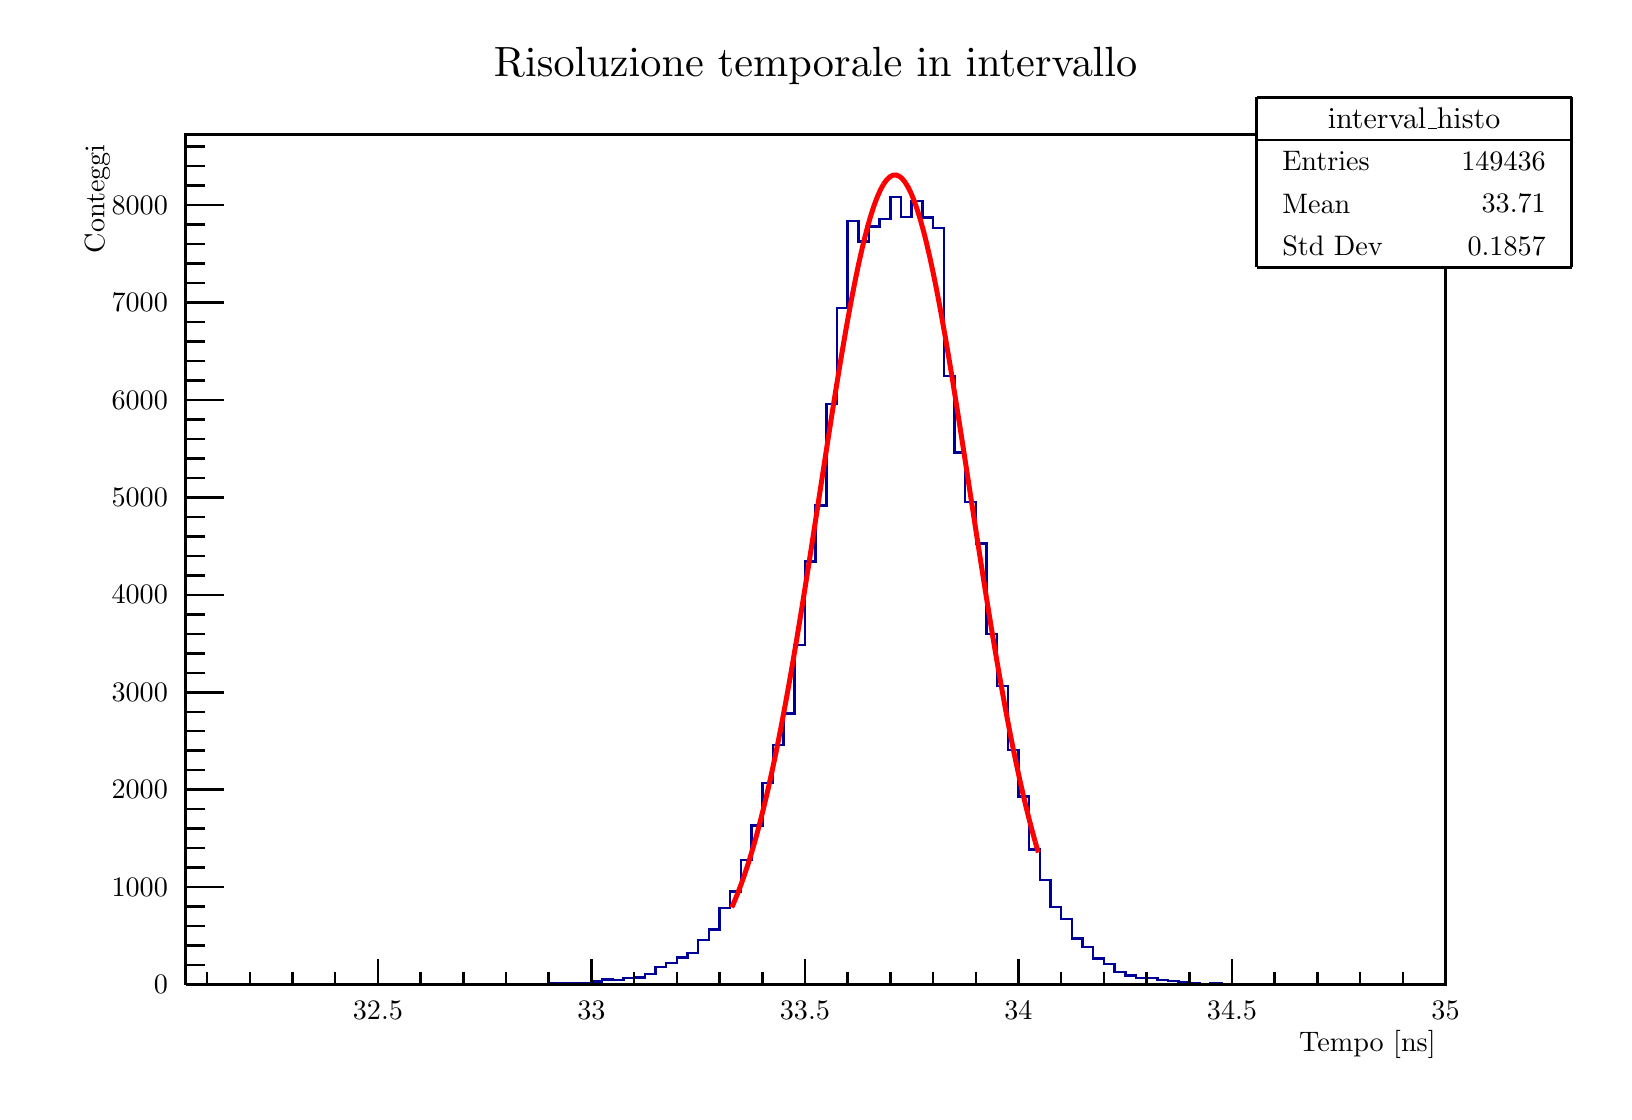
\begin{tikzpicture}
\pgfdeclareplotmark{cross} {
\pgfpathmoveto{\pgfpoint{-0.3\pgfplotmarksize}{\pgfplotmarksize}}
\pgfpathlineto{\pgfpoint{+0.3\pgfplotmarksize}{\pgfplotmarksize}}
\pgfpathlineto{\pgfpoint{+0.3\pgfplotmarksize}{0.3\pgfplotmarksize}}
\pgfpathlineto{\pgfpoint{+1\pgfplotmarksize}{0.3\pgfplotmarksize}}
\pgfpathlineto{\pgfpoint{+1\pgfplotmarksize}{-0.3\pgfplotmarksize}}
\pgfpathlineto{\pgfpoint{+0.3\pgfplotmarksize}{-0.3\pgfplotmarksize}}
\pgfpathlineto{\pgfpoint{+0.3\pgfplotmarksize}{-1.\pgfplotmarksize}}
\pgfpathlineto{\pgfpoint{-0.3\pgfplotmarksize}{-1.\pgfplotmarksize}}
\pgfpathlineto{\pgfpoint{-0.3\pgfplotmarksize}{-0.3\pgfplotmarksize}}
\pgfpathlineto{\pgfpoint{-1.\pgfplotmarksize}{-0.3\pgfplotmarksize}}
\pgfpathlineto{\pgfpoint{-1.\pgfplotmarksize}{0.3\pgfplotmarksize}}
\pgfpathlineto{\pgfpoint{-0.3\pgfplotmarksize}{0.3\pgfplotmarksize}}
\pgfpathclose
\pgfusepathqstroke
}
\pgfdeclareplotmark{cross*} {
\pgfpathmoveto{\pgfpoint{-0.3\pgfplotmarksize}{\pgfplotmarksize}}
\pgfpathlineto{\pgfpoint{+0.3\pgfplotmarksize}{\pgfplotmarksize}}
\pgfpathlineto{\pgfpoint{+0.3\pgfplotmarksize}{0.3\pgfplotmarksize}}
\pgfpathlineto{\pgfpoint{+1\pgfplotmarksize}{0.3\pgfplotmarksize}}
\pgfpathlineto{\pgfpoint{+1\pgfplotmarksize}{-0.3\pgfplotmarksize}}
\pgfpathlineto{\pgfpoint{+0.3\pgfplotmarksize}{-0.3\pgfplotmarksize}}
\pgfpathlineto{\pgfpoint{+0.3\pgfplotmarksize}{-1.\pgfplotmarksize}}
\pgfpathlineto{\pgfpoint{-0.3\pgfplotmarksize}{-1.\pgfplotmarksize}}
\pgfpathlineto{\pgfpoint{-0.3\pgfplotmarksize}{-0.3\pgfplotmarksize}}
\pgfpathlineto{\pgfpoint{-1.\pgfplotmarksize}{-0.3\pgfplotmarksize}}
\pgfpathlineto{\pgfpoint{-1.\pgfplotmarksize}{0.3\pgfplotmarksize}}
\pgfpathlineto{\pgfpoint{-0.3\pgfplotmarksize}{0.3\pgfplotmarksize}}
\pgfpathclose
\pgfusepathqfillstroke
}
\pgfdeclareplotmark{newstar} {
\pgfpathmoveto{\pgfqpoint{0pt}{\pgfplotmarksize}}
\pgfpathlineto{\pgfqpointpolar{44}{0.5\pgfplotmarksize}}
\pgfpathlineto{\pgfqpointpolar{18}{\pgfplotmarksize}}
\pgfpathlineto{\pgfqpointpolar{-20}{0.5\pgfplotmarksize}}
\pgfpathlineto{\pgfqpointpolar{-54}{\pgfplotmarksize}}
\pgfpathlineto{\pgfqpointpolar{-90}{0.5\pgfplotmarksize}}
\pgfpathlineto{\pgfqpointpolar{234}{\pgfplotmarksize}}
\pgfpathlineto{\pgfqpointpolar{198}{0.5\pgfplotmarksize}}
\pgfpathlineto{\pgfqpointpolar{162}{\pgfplotmarksize}}
\pgfpathlineto{\pgfqpointpolar{134}{0.5\pgfplotmarksize}}
\pgfpathclose
\pgfusepathqstroke
}
\pgfdeclareplotmark{newstar*} {
\pgfpathmoveto{\pgfqpoint{0pt}{\pgfplotmarksize}}
\pgfpathlineto{\pgfqpointpolar{44}{0.5\pgfplotmarksize}}
\pgfpathlineto{\pgfqpointpolar{18}{\pgfplotmarksize}}
\pgfpathlineto{\pgfqpointpolar{-20}{0.5\pgfplotmarksize}}
\pgfpathlineto{\pgfqpointpolar{-54}{\pgfplotmarksize}}
\pgfpathlineto{\pgfqpointpolar{-90}{0.5\pgfplotmarksize}}
\pgfpathlineto{\pgfqpointpolar{234}{\pgfplotmarksize}}
\pgfpathlineto{\pgfqpointpolar{198}{0.5\pgfplotmarksize}}
\pgfpathlineto{\pgfqpointpolar{162}{\pgfplotmarksize}}
\pgfpathlineto{\pgfqpointpolar{134}{0.5\pgfplotmarksize}}
\pgfpathclose
\pgfusepathqfillstroke
}
\definecolor{c}{rgb}{1,1,1};
\draw [color=c, fill=c] (0,0) rectangle (20,13.4957);
\draw [color=c, fill=c] (2,1.34957) rectangle (18,12.1461);
\definecolor{c}{rgb}{0,0,0};
\draw [c,line width=0.9] (2,1.34957) -- (2,12.1461) -- (18,12.1461) -- (18,1.34957) -- (2,1.34957);
\definecolor{c}{rgb}{1,1,1};
\draw [color=c, fill=c] (2,1.34957) rectangle (18,12.1461);
\definecolor{c}{rgb}{0,0,0};
\draw [c,line width=0.9] (2,1.34957) -- (2,12.1461) -- (18,12.1461) -- (18,1.34957) -- (2,1.34957);
\definecolor{c}{rgb}{0,0,0.6};
\draw [c,line width=0.9] (2,1.34957) -- (2.13559,1.34957) -- (2.13559,1.35081) -- (2.27119,1.35081) -- (2.27119,1.34957) -- (2.40678,1.34957) -- (2.40678,1.35081) -- (2.54237,1.35081) -- (2.54237,1.34957) -- (2.67797,1.34957) -- (2.67797,1.34957) --
 (2.81356,1.34957) -- (2.81356,1.34957) -- (2.94915,1.34957) -- (2.94915,1.35081) -- (3.08475,1.35081) -- (3.08475,1.35081) -- (3.22034,1.35081) -- (3.22034,1.35081) -- (3.35593,1.35081) -- (3.35593,1.35081) -- (3.49153,1.35081) -- (3.49153,1.35081)
 -- (3.62712,1.35081) -- (3.62712,1.34957) -- (3.76271,1.34957) -- (3.76271,1.35081) -- (3.89831,1.35081) -- (3.89831,1.34957) -- (4.0339,1.34957) -- (4.0339,1.35205) -- (4.16949,1.35205) -- (4.16949,1.35081) -- (4.30508,1.35081) -- (4.30508,1.34957)
 -- (4.44068,1.34957) -- (4.44068,1.35205) -- (4.57627,1.35205) -- (4.57627,1.35328) -- (4.71186,1.35328) -- (4.71186,1.35081) -- (4.84746,1.35081) -- (4.84746,1.35205) -- (4.98305,1.35205) -- (4.98305,1.35081) -- (5.11864,1.35081) --
 (5.11864,1.35328) -- (5.25424,1.35328) -- (5.25424,1.35205) -- (5.38983,1.35205) -- (5.38983,1.35205) -- (5.52542,1.35205) -- (5.52542,1.35081) -- (5.66102,1.35081) -- (5.66102,1.35452) -- (5.79661,1.35452) -- (5.79661,1.34957) -- (5.9322,1.34957)
 -- (5.9322,1.357) -- (6.0678,1.357) -- (6.0678,1.357) -- (6.20339,1.357) -- (6.20339,1.35576) -- (6.33898,1.35576) -- (6.33898,1.35328) -- (6.47458,1.35328) -- (6.47458,1.35947) -- (6.61017,1.35947) -- (6.61017,1.36071) -- (6.74576,1.36071) --
 (6.74576,1.3669) -- (6.88136,1.3669) -- (6.88136,1.36937) -- (7.01695,1.36937) -- (7.01695,1.36937) -- (7.15254,1.36937) -- (7.15254,1.38793) -- (7.28814,1.38793) -- (7.28814,1.41269) -- (7.42373,1.41269) -- (7.42373,1.4065) -- (7.55932,1.4065) --
 (7.55932,1.43496) -- (7.69492,1.43496) -- (7.69492,1.44239) -- (7.83051,1.44239) -- (7.83051,1.48446) -- (7.9661,1.48446) -- (7.9661,1.57357) -- (8.1017,1.57357) -- (8.1017,1.62183) -- (8.23729,1.62183) -- (8.23729,1.69609) -- (8.37288,1.69609) --
 (8.37288,1.75301) -- (8.50847,1.75301) -- (8.50847,1.9139) -- (8.64407,1.9139) -- (8.64407,2.0525) -- (8.77966,2.0525) -- (8.77966,2.31982) -- (8.91525,2.31982) -- (8.91525,2.53515) -- (9.05085,2.53515) -- (9.05085,2.93365) -- (9.18644,2.93365) --
 (9.18644,3.36803) -- (9.32203,3.36803) -- (9.32203,3.90761) -- (9.45763,3.90761) -- (9.45763,4.39026) -- (9.59322,4.39026) -- (9.59322,4.78999) -- (9.72881,4.78999) -- (9.72881,5.66371) -- (9.86441,5.66371) -- (9.86441,6.72306) -- (10,6.72306) --
 (10,7.43218) -- (10.1356,7.43218) -- (10.1356,8.72048) -- (10.2712,8.72048) -- (10.2712,9.94195) -- (10.4068,9.94195) -- (10.4068,11.0496) -- (10.5424,11.0496) -- (10.5424,10.7884) -- (10.678,10.7884) -- (10.678,10.9766) -- (10.8136,10.9766) --
 (10.8136,11.0718) -- (10.9492,11.0718) -- (10.9492,11.3528) -- (11.0847,11.3528) -- (11.0847,11.0966) -- (11.2203,11.0966) -- (11.2203,11.3033) -- (11.3559,11.3033) -- (11.3559,11.0929) -- (11.4915,11.0929) -- (11.4915,10.9605) -- (11.6271,10.9605)
 -- (11.6271,9.08185) -- (11.7627,9.08185) -- (11.7627,8.10541) -- (11.8983,8.10541) -- (11.8983,7.47549) -- (12.0339,7.47549) -- (12.0339,6.95448) -- (12.1695,6.95448) -- (12.1695,5.80108) -- (12.3051,5.80108) -- (12.3051,5.14269) --
 (12.4407,5.14269) -- (12.4407,4.33085) -- (12.5763,4.33085) -- (12.5763,3.73682) -- (12.7119,3.73682) -- (12.7119,3.06359) -- (12.8475,3.06359) -- (12.8475,2.68119) -- (12.9831,2.68119) -- (12.9831,2.33219) -- (13.1186,2.33219) -- (13.1186,2.18245)
 -- (13.2542,2.18245) -- (13.2542,1.9337) -- (13.3898,1.9337) -- (13.3898,1.82479) -- (13.5254,1.82479) -- (13.5254,1.68371) -- (13.661,1.68371) -- (13.661,1.60946) -- (13.7966,1.60946) -- (13.7966,1.51293) -- (13.9322,1.51293) -- (13.9322,1.46838)
 -- (14.0678,1.46838) -- (14.0678,1.43125) -- (14.2034,1.43125) -- (14.2034,1.4362) -- (14.339,1.4362) -- (14.339,1.40526) -- (14.4746,1.40526) -- (14.4746,1.39784) -- (14.6102,1.39784) -- (14.6102,1.37927) -- (14.7458,1.37927) -- (14.7458,1.37308)
 -- (14.8814,1.37308) -- (14.8814,1.35823) -- (15.0169,1.35823) -- (15.0169,1.3669) -- (15.1525,1.3669) -- (15.1525,1.357) -- (15.2881,1.357) -- (15.2881,1.35823) -- (15.4237,1.35823) -- (15.4237,1.35328) -- (15.5593,1.35328) -- (15.5593,1.35081) --
 (15.6949,1.35081) -- (15.6949,1.35328) -- (15.8305,1.35328) -- (15.8305,1.35081) -- (15.9661,1.35081) -- (15.9661,1.35205) -- (16.1017,1.35205) -- (16.1017,1.34957) -- (16.2373,1.34957) -- (16.2373,1.35081) -- (16.3729,1.35081) -- (16.3729,1.35081)
 -- (16.5085,1.35081) -- (16.5085,1.35205) -- (16.6441,1.35205) -- (16.6441,1.34957) -- (16.7797,1.34957) -- (16.7797,1.35081) -- (16.9153,1.35081) -- (16.9153,1.35205) -- (17.0508,1.35205) -- (17.0508,1.34957) -- (17.1864,1.34957) --
 (17.1864,1.34957) -- (17.322,1.34957) -- (17.322,1.35081) -- (17.4576,1.35081) -- (17.4576,1.34957) -- (17.5932,1.34957) -- (17.5932,1.34957) -- (17.7288,1.34957) -- (17.7288,1.35081) -- (17.8644,1.35081) -- (17.8644,1.35081) -- (18,1.35081);
\definecolor{c}{rgb}{1,1,1};
\draw [color=c, fill=c] (15.6,10.4592) rectangle (19.6,12.6185);
\definecolor{c}{rgb}{0,0,0};
\draw [c,line width=0.9] (15.6,10.4592) -- (19.6,10.4592);
\draw [c,line width=0.9] (19.6,10.4592) -- (19.6,12.6185);
\draw [c,line width=0.9] (19.6,12.6185) -- (15.6,12.6185);
\draw [c,line width=0.9] (15.6,12.6185) -- (15.6,10.4592);
\draw (17.6,12.3486) node[scale=1.08185, color=c, rotate=0]{interval\_histo};
\draw [c,line width=0.9] (15.6,12.0787) -- (19.6,12.0787);
\draw [anchor= west] (15.8,11.8087) node[scale=1.01821, color=c, rotate=0]{Entries };
\draw [anchor= east] (19.4,11.8087) node[scale=1.01821, color=c, rotate=0]{ 149436};
\draw [anchor= west] (15.8,11.2689) node[scale=1.01821, color=c, rotate=0]{Mean  };
\draw [anchor= east] (19.4,11.2689) node[scale=1.01821, color=c, rotate=0]{  33.71};
\draw [anchor= west] (15.8,10.7291) node[scale=1.01821, color=c, rotate=0]{Std Dev   };
\draw [anchor= east] (19.4,10.7291) node[scale=1.01821, color=c, rotate=0]{ 0.1857};
\definecolor{c}{rgb}{1,0,0};
\draw [c,line width=1.8] (8.93492,2.32999) -- (8.97424,2.42054) -- (9.01356,2.51746) -- (9.05288,2.62101) -- (9.0922,2.7314) -- (9.13153,2.84883) -- (9.17085,2.97349) -- (9.21017,3.10555) -- (9.24949,3.24513) -- (9.28881,3.39235) -- (9.32814,3.54729)
 -- (9.36746,3.70997) -- (9.40678,3.88042) -- (9.4461,4.05858) -- (9.48542,4.24439) -- (9.52475,4.4377) -- (9.56407,4.63836) -- (9.60339,4.84614) -- (9.64271,5.06076) -- (9.68203,5.2819) -- (9.72136,5.50917) -- (9.76068,5.74213) -- (9.8,5.9803) --
 (9.83932,6.22314) -- (9.87864,6.47003) -- (9.91797,6.72034) -- (9.95729,6.97337) -- (9.99661,7.22835) -- (10.0359,7.48451) -- (10.0753,7.74101) -- (10.1146,7.99698) -- (10.1539,8.25152) -- (10.1932,8.50368) -- (10.2325,8.75252) -- (10.2719,8.99707)
 -- (10.3112,9.23634) -- (10.3505,9.46935) -- (10.3898,9.6951) -- (10.4292,9.91264) -- (10.4685,10.121) -- (10.5078,10.3192) -- (10.5471,10.5064) -- (10.5864,10.6818) -- (10.6258,10.8443) -- (10.6651,10.9934) -- (10.7044,11.1283) -- (10.7437,11.2483)
 -- (10.7831,11.3529) -- (10.8224,11.4414) -- (10.8617,11.5135);
\draw [c,line width=1.8] (10.8617,11.5135) -- (10.901,11.5689) -- (10.9403,11.6071) -- (10.9797,11.6281) -- (11.019,11.6318) -- (11.0583,11.618) -- (11.0976,11.587) -- (11.1369,11.5387) -- (11.1763,11.4736) -- (11.2156,11.3919) -- (11.2549,11.2939)
 -- (11.2942,11.1803) -- (11.3336,11.0516) -- (11.3729,10.9084) -- (11.4122,10.7513) -- (11.4515,10.5812) -- (11.4908,10.3989) -- (11.5302,10.2052) -- (11.5695,10.0009) -- (11.6088,9.78713) -- (11.6481,9.56469) -- (11.6875,9.33459) --
 (11.7268,9.09782) -- (11.7661,8.85536) -- (11.8054,8.6082) -- (11.8447,8.3573) -- (11.8841,8.10365) -- (11.9234,7.84817) -- (11.9627,7.59178) -- (12.002,7.33538) -- (12.0414,7.0798) -- (12.0807,6.82586) -- (12.12,6.57433) -- (12.1593,6.32592) --
 (12.1986,6.08131) -- (12.238,5.84112) -- (12.2773,5.60592) -- (12.3166,5.37621) -- (12.3559,5.15246) -- (12.3953,4.93507) -- (12.4346,4.7244) -- (12.4739,4.52073) -- (12.5132,4.32432) -- (12.5525,4.13535) -- (12.5919,3.95398) -- (12.6312,3.7803) --
 (12.6705,3.61437) -- (12.7098,3.4562) -- (12.7492,3.30576) -- (12.7885,3.163);
\draw [c,line width=1.8] (12.7885,3.163) -- (12.8278,3.02781);
\definecolor{c}{rgb}{0,0,0};
\draw [c,line width=0.9] (2,1.34957) -- (18,1.34957);
\draw [anchor= east] (18,0.593811) node[scale=1.01821, color=c, rotate=0]{Tempo [ns]};
\draw [c,line width=0.9] (4.44068,1.67347) -- (4.44068,1.34957);
\draw [c,line width=0.9] (4.98305,1.51152) -- (4.98305,1.34957);
\draw [c,line width=0.9] (5.52542,1.51152) -- (5.52542,1.34957);
\draw [c,line width=0.9] (6.0678,1.51152) -- (6.0678,1.34957);
\draw [c,line width=0.9] (6.61017,1.51152) -- (6.61017,1.34957);
\draw [c,line width=0.9] (7.15254,1.67347) -- (7.15254,1.34957);
\draw [c,line width=0.9] (7.69492,1.51152) -- (7.69492,1.34957);
\draw [c,line width=0.9] (8.23729,1.51152) -- (8.23729,1.34957);
\draw [c,line width=0.9] (8.77966,1.51152) -- (8.77966,1.34957);
\draw [c,line width=0.9] (9.32203,1.51152) -- (9.32203,1.34957);
\draw [c,line width=0.9] (9.86441,1.67347) -- (9.86441,1.34957);
\draw [c,line width=0.9] (10.4068,1.51152) -- (10.4068,1.34957);
\draw [c,line width=0.9] (10.9492,1.51152) -- (10.9492,1.34957);
\draw [c,line width=0.9] (11.4915,1.51152) -- (11.4915,1.34957);
\draw [c,line width=0.9] (12.0339,1.51152) -- (12.0339,1.34957);
\draw [c,line width=0.9] (12.5763,1.67347) -- (12.5763,1.34957);
\draw [c,line width=0.9] (13.1186,1.51152) -- (13.1186,1.34957);
\draw [c,line width=0.9] (13.661,1.51152) -- (13.661,1.34957);
\draw [c,line width=0.9] (14.2034,1.51152) -- (14.2034,1.34957);
\draw [c,line width=0.9] (14.7458,1.51152) -- (14.7458,1.34957);
\draw [c,line width=0.9] (15.2881,1.67347) -- (15.2881,1.34957);
\draw [c,line width=0.9] (15.8305,1.51152) -- (15.8305,1.34957);
\draw [c,line width=0.9] (16.3729,1.51152) -- (16.3729,1.34957);
\draw [c,line width=0.9] (16.9153,1.51152) -- (16.9153,1.34957);
\draw [c,line width=0.9] (17.4576,1.51152) -- (17.4576,1.34957);
\draw [c,line width=0.9] (18,1.67347) -- (18,1.34957);
\draw [c,line width=0.9] (4.44068,1.67347) -- (4.44068,1.34957);
\draw [c,line width=0.9] (3.89831,1.51152) -- (3.89831,1.34957);
\draw [c,line width=0.9] (3.35593,1.51152) -- (3.35593,1.34957);
\draw [c,line width=0.9] (2.81356,1.51152) -- (2.81356,1.34957);
\draw [c,line width=0.9] (2.27119,1.51152) -- (2.27119,1.34957);
\draw [anchor=base] (4.44068,0.904212) node[scale=1.01821, color=c, rotate=0]{32.5};
\draw [anchor=base] (7.15254,0.904212) node[scale=1.01821, color=c, rotate=0]{33};
\draw [anchor=base] (9.86441,0.904212) node[scale=1.01821, color=c, rotate=0]{33.5};
\draw [anchor=base] (12.5763,0.904212) node[scale=1.01821, color=c, rotate=0]{34};
\draw [anchor=base] (15.2881,0.904212) node[scale=1.01821, color=c, rotate=0]{34.5};
\draw [anchor=base] (18,0.904212) node[scale=1.01821, color=c, rotate=0]{35};
\draw [c,line width=0.9] (2,1.34957) -- (2,12.1461);
\draw [anchor= east] (0.88,12.1461) node[scale=1.01821, color=c, rotate=90]{Conteggi};
\draw [c,line width=0.9] (2.48,1.34957) -- (2,1.34957);
\draw [c,line width=0.9] (2.24,1.59708) -- (2,1.59708);
\draw [c,line width=0.9] (2.24,1.84459) -- (2,1.84459);
\draw [c,line width=0.9] (2.24,2.09211) -- (2,2.09211);
\draw [c,line width=0.9] (2.24,2.33962) -- (2,2.33962);
\draw [c,line width=0.9] (2.48,2.58713) -- (2,2.58713);
\draw [c,line width=0.9] (2.24,2.83464) -- (2,2.83464);
\draw [c,line width=0.9] (2.24,3.08215) -- (2,3.08215);
\draw [c,line width=0.9] (2.24,3.32967) -- (2,3.32967);
\draw [c,line width=0.9] (2.24,3.57718) -- (2,3.57718);
\draw [c,line width=0.9] (2.48,3.82469) -- (2,3.82469);
\draw [c,line width=0.9] (2.24,4.0722) -- (2,4.0722);
\draw [c,line width=0.9] (2.24,4.31972) -- (2,4.31972);
\draw [c,line width=0.9] (2.24,4.56723) -- (2,4.56723);
\draw [c,line width=0.9] (2.24,4.81474) -- (2,4.81474);
\draw [c,line width=0.9] (2.48,5.06225) -- (2,5.06225);
\draw [c,line width=0.9] (2.24,5.30976) -- (2,5.30976);
\draw [c,line width=0.9] (2.24,5.55728) -- (2,5.55728);
\draw [c,line width=0.9] (2.24,5.80479) -- (2,5.80479);
\draw [c,line width=0.9] (2.24,6.0523) -- (2,6.0523);
\draw [c,line width=0.9] (2.48,6.29981) -- (2,6.29981);
\draw [c,line width=0.9] (2.24,6.54732) -- (2,6.54732);
\draw [c,line width=0.9] (2.24,6.79484) -- (2,6.79484);
\draw [c,line width=0.9] (2.24,7.04235) -- (2,7.04235);
\draw [c,line width=0.9] (2.24,7.28986) -- (2,7.28986);
\draw [c,line width=0.9] (2.48,7.53737) -- (2,7.53737);
\draw [c,line width=0.9] (2.24,7.78488) -- (2,7.78488);
\draw [c,line width=0.9] (2.24,8.0324) -- (2,8.0324);
\draw [c,line width=0.9] (2.24,8.27991) -- (2,8.27991);
\draw [c,line width=0.9] (2.24,8.52742) -- (2,8.52742);
\draw [c,line width=0.9] (2.48,8.77493) -- (2,8.77493);
\draw [c,line width=0.9] (2.24,9.02244) -- (2,9.02244);
\draw [c,line width=0.9] (2.24,9.26996) -- (2,9.26996);
\draw [c,line width=0.9] (2.24,9.51747) -- (2,9.51747);
\draw [c,line width=0.9] (2.24,9.76498) -- (2,9.76498);
\draw [c,line width=0.9] (2.48,10.0125) -- (2,10.0125);
\draw [c,line width=0.9] (2.24,10.26) -- (2,10.26);
\draw [c,line width=0.9] (2.24,10.5075) -- (2,10.5075);
\draw [c,line width=0.9] (2.24,10.755) -- (2,10.755);
\draw [c,line width=0.9] (2.24,11.0025) -- (2,11.0025);
\draw [c,line width=0.9] (2.48,11.2501) -- (2,11.2501);
\draw [c,line width=0.9] (2.48,11.2501) -- (2,11.2501);
\draw [c,line width=0.9] (2.24,11.4976) -- (2,11.4976);
\draw [c,line width=0.9] (2.24,11.7451) -- (2,11.7451);
\draw [c,line width=0.9] (2.24,11.9926) -- (2,11.9926);
\draw [anchor= east] (1.9,1.34957) node[scale=1.01821, color=c, rotate=0]{0};
\draw [anchor= east] (1.9,2.58713) node[scale=1.01821, color=c, rotate=0]{1000};
\draw [anchor= east] (1.9,3.82469) node[scale=1.01821, color=c, rotate=0]{2000};
\draw [anchor= east] (1.9,5.06225) node[scale=1.01821, color=c, rotate=0]{3000};
\draw [anchor= east] (1.9,6.29981) node[scale=1.01821, color=c, rotate=0]{4000};
\draw [anchor= east] (1.9,7.53737) node[scale=1.01821, color=c, rotate=0]{5000};
\draw [anchor= east] (1.9,8.77493) node[scale=1.01821, color=c, rotate=0]{6000};
\draw [anchor= east] (1.9,10.0125) node[scale=1.01821, color=c, rotate=0]{7000};
\draw [anchor= east] (1.9,11.2501) node[scale=1.01821, color=c, rotate=0]{8000};
\definecolor{c}{rgb}{1,1,1};
\draw [color=c, fill=c] (15.6,10.4592) rectangle (19.6,12.6185);
\definecolor{c}{rgb}{0,0,0};
\draw [c,line width=0.9] (15.6,10.4592) -- (19.6,10.4592);
\draw [c,line width=0.9] (19.6,10.4592) -- (19.6,12.6185);
\draw [c,line width=0.9] (19.6,12.6185) -- (15.6,12.6185);
\draw [c,line width=0.9] (15.6,12.6185) -- (15.6,10.4592);
\draw (17.6,12.3486) node[scale=1.08185, color=c, rotate=0]{interval\_histo};
\draw [c,line width=0.9] (15.6,12.0787) -- (19.6,12.0787);
\draw [anchor= west] (15.8,11.8087) node[scale=1.01821, color=c, rotate=0]{Entries };
\draw [anchor= east] (19.4,11.8087) node[scale=1.01821, color=c, rotate=0]{ 149436};
\draw [anchor= west] (15.8,11.2689) node[scale=1.01821, color=c, rotate=0]{Mean  };
\draw [anchor= east] (19.4,11.2689) node[scale=1.01821, color=c, rotate=0]{  33.71};
\draw [anchor= west] (15.8,10.7291) node[scale=1.01821, color=c, rotate=0]{Std Dev   };
\draw [anchor= east] (19.4,10.7291) node[scale=1.01821, color=c, rotate=0]{ 0.1857};
\draw (10,13.0156) node[scale=1.52731, color=c, rotate=0]{Risoluzione temporale in intervallo};
\end{tikzpicture}

%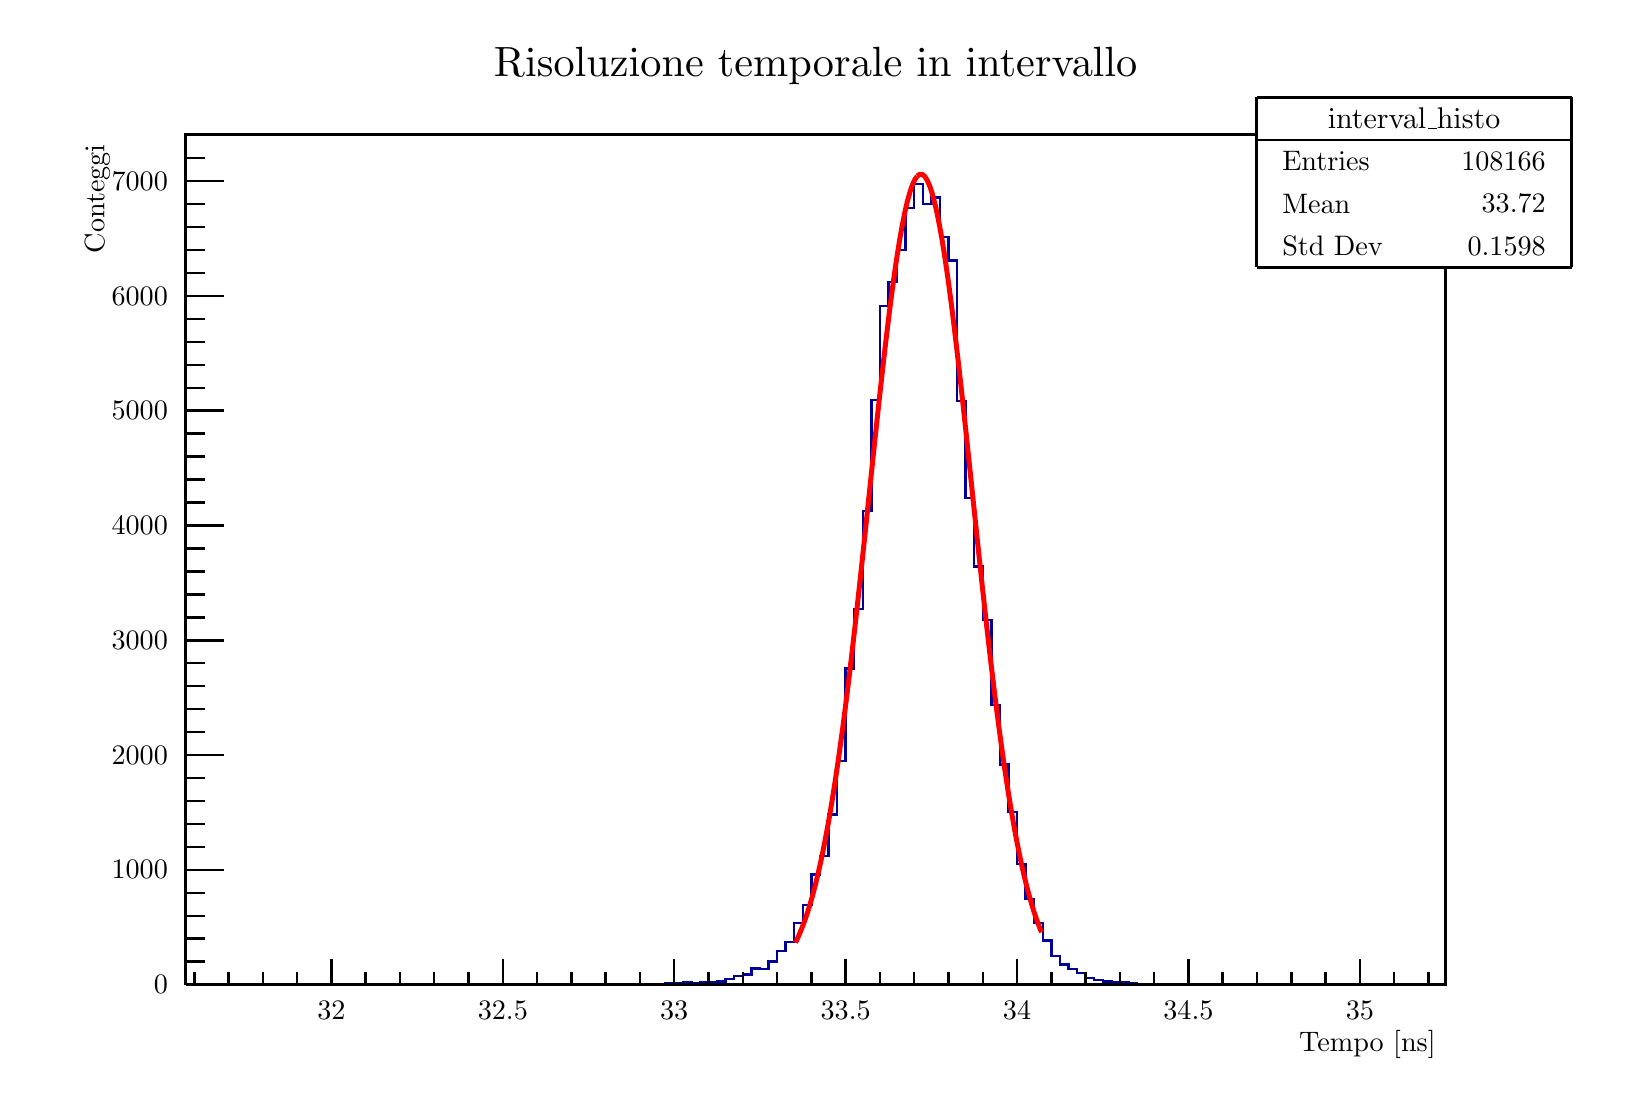
\begin{tikzpicture}
\pgfdeclareplotmark{cross} {
\pgfpathmoveto{\pgfpoint{-0.3\pgfplotmarksize}{\pgfplotmarksize}}
\pgfpathlineto{\pgfpoint{+0.3\pgfplotmarksize}{\pgfplotmarksize}}
\pgfpathlineto{\pgfpoint{+0.3\pgfplotmarksize}{0.3\pgfplotmarksize}}
\pgfpathlineto{\pgfpoint{+1\pgfplotmarksize}{0.3\pgfplotmarksize}}
\pgfpathlineto{\pgfpoint{+1\pgfplotmarksize}{-0.3\pgfplotmarksize}}
\pgfpathlineto{\pgfpoint{+0.3\pgfplotmarksize}{-0.3\pgfplotmarksize}}
\pgfpathlineto{\pgfpoint{+0.3\pgfplotmarksize}{-1.\pgfplotmarksize}}
\pgfpathlineto{\pgfpoint{-0.3\pgfplotmarksize}{-1.\pgfplotmarksize}}
\pgfpathlineto{\pgfpoint{-0.3\pgfplotmarksize}{-0.3\pgfplotmarksize}}
\pgfpathlineto{\pgfpoint{-1.\pgfplotmarksize}{-0.3\pgfplotmarksize}}
\pgfpathlineto{\pgfpoint{-1.\pgfplotmarksize}{0.3\pgfplotmarksize}}
\pgfpathlineto{\pgfpoint{-0.3\pgfplotmarksize}{0.3\pgfplotmarksize}}
\pgfpathclose
\pgfusepathqstroke
}
\pgfdeclareplotmark{cross*} {
\pgfpathmoveto{\pgfpoint{-0.3\pgfplotmarksize}{\pgfplotmarksize}}
\pgfpathlineto{\pgfpoint{+0.3\pgfplotmarksize}{\pgfplotmarksize}}
\pgfpathlineto{\pgfpoint{+0.3\pgfplotmarksize}{0.3\pgfplotmarksize}}
\pgfpathlineto{\pgfpoint{+1\pgfplotmarksize}{0.3\pgfplotmarksize}}
\pgfpathlineto{\pgfpoint{+1\pgfplotmarksize}{-0.3\pgfplotmarksize}}
\pgfpathlineto{\pgfpoint{+0.3\pgfplotmarksize}{-0.3\pgfplotmarksize}}
\pgfpathlineto{\pgfpoint{+0.3\pgfplotmarksize}{-1.\pgfplotmarksize}}
\pgfpathlineto{\pgfpoint{-0.3\pgfplotmarksize}{-1.\pgfplotmarksize}}
\pgfpathlineto{\pgfpoint{-0.3\pgfplotmarksize}{-0.3\pgfplotmarksize}}
\pgfpathlineto{\pgfpoint{-1.\pgfplotmarksize}{-0.3\pgfplotmarksize}}
\pgfpathlineto{\pgfpoint{-1.\pgfplotmarksize}{0.3\pgfplotmarksize}}
\pgfpathlineto{\pgfpoint{-0.3\pgfplotmarksize}{0.3\pgfplotmarksize}}
\pgfpathclose
\pgfusepathqfillstroke
}
\pgfdeclareplotmark{newstar} {
\pgfpathmoveto{\pgfqpoint{0pt}{\pgfplotmarksize}}
\pgfpathlineto{\pgfqpointpolar{44}{0.5\pgfplotmarksize}}
\pgfpathlineto{\pgfqpointpolar{18}{\pgfplotmarksize}}
\pgfpathlineto{\pgfqpointpolar{-20}{0.5\pgfplotmarksize}}
\pgfpathlineto{\pgfqpointpolar{-54}{\pgfplotmarksize}}
\pgfpathlineto{\pgfqpointpolar{-90}{0.5\pgfplotmarksize}}
\pgfpathlineto{\pgfqpointpolar{234}{\pgfplotmarksize}}
\pgfpathlineto{\pgfqpointpolar{198}{0.5\pgfplotmarksize}}
\pgfpathlineto{\pgfqpointpolar{162}{\pgfplotmarksize}}
\pgfpathlineto{\pgfqpointpolar{134}{0.5\pgfplotmarksize}}
\pgfpathclose
\pgfusepathqstroke
}
\pgfdeclareplotmark{newstar*} {
\pgfpathmoveto{\pgfqpoint{0pt}{\pgfplotmarksize}}
\pgfpathlineto{\pgfqpointpolar{44}{0.5\pgfplotmarksize}}
\pgfpathlineto{\pgfqpointpolar{18}{\pgfplotmarksize}}
\pgfpathlineto{\pgfqpointpolar{-20}{0.5\pgfplotmarksize}}
\pgfpathlineto{\pgfqpointpolar{-54}{\pgfplotmarksize}}
\pgfpathlineto{\pgfqpointpolar{-90}{0.5\pgfplotmarksize}}
\pgfpathlineto{\pgfqpointpolar{234}{\pgfplotmarksize}}
\pgfpathlineto{\pgfqpointpolar{198}{0.5\pgfplotmarksize}}
\pgfpathlineto{\pgfqpointpolar{162}{\pgfplotmarksize}}
\pgfpathlineto{\pgfqpointpolar{134}{0.5\pgfplotmarksize}}
\pgfpathclose
\pgfusepathqfillstroke
}
\definecolor{c}{rgb}{1,1,1};
\draw [color=c, fill=c] (0,0) rectangle (20,13.4957);
\draw [color=c, fill=c] (2,1.34957) rectangle (18,12.1461);
\definecolor{c}{rgb}{0,0,0};
\draw [c,line width=0.9] (2,1.34957) -- (2,12.1461) -- (18,12.1461) -- (18,1.34957) -- (2,1.34957);
\definecolor{c}{rgb}{1,1,1};
\draw [color=c, fill=c] (2,1.34957) rectangle (18,12.1461);
\definecolor{c}{rgb}{0,0,0};
\draw [c,line width=0.9] (2,1.34957) -- (2,12.1461) -- (18,12.1461) -- (18,1.34957) -- (2,1.34957);
\definecolor{c}{rgb}{0,0,0.6};
\draw [c,line width=0.9] (2,1.34957) -- (2.10884,1.34957) -- (2.10884,1.35103) -- (2.21769,1.35103) -- (2.21769,1.34957) -- (2.32653,1.34957) -- (2.32653,1.34957) -- (2.43537,1.34957) -- (2.43537,1.34957) -- (2.54422,1.34957) -- (2.54422,1.34957) --
 (2.65306,1.34957) -- (2.65306,1.35103) -- (2.7619,1.35103) -- (2.7619,1.34957) -- (2.87075,1.34957) -- (2.87075,1.34957) -- (2.97959,1.34957) -- (2.97959,1.35249) -- (3.08844,1.35249) -- (3.08844,1.35103) -- (3.19728,1.35103) -- (3.19728,1.35103) --
 (3.30612,1.35103) -- (3.30612,1.34957) -- (3.41497,1.34957) -- (3.41497,1.34957) -- (3.52381,1.34957) -- (3.52381,1.34957) -- (3.63265,1.34957) -- (3.63265,1.34957) -- (3.7415,1.34957) -- (3.7415,1.35103) -- (3.85034,1.35103) -- (3.85034,1.34957) --
 (3.95918,1.34957) -- (3.95918,1.35103) -- (4.06803,1.35103) -- (4.06803,1.35103) -- (4.17687,1.35103) -- (4.17687,1.34957) -- (4.28571,1.34957) -- (4.28571,1.34957) -- (4.39456,1.34957) -- (4.39456,1.34957) -- (4.5034,1.34957) -- (4.5034,1.34957) --
 (4.61225,1.34957) -- (4.61225,1.35249) -- (4.72109,1.35249) -- (4.72109,1.35103) -- (4.82993,1.35103) -- (4.82993,1.34957) -- (4.93878,1.34957) -- (4.93878,1.34957) -- (5.04762,1.34957) -- (5.04762,1.35249) -- (5.15646,1.35249) -- (5.15646,1.34957)
 -- (5.26531,1.34957) -- (5.26531,1.34957) -- (5.37415,1.34957) -- (5.37415,1.35103) -- (5.48299,1.35103) -- (5.48299,1.35103) -- (5.59184,1.35103) -- (5.59184,1.34957) -- (5.70068,1.34957) -- (5.70068,1.35394) -- (5.80952,1.35394) --
 (5.80952,1.34957) -- (5.91837,1.34957) -- (5.91837,1.34957) -- (6.02721,1.34957) -- (6.02721,1.34957) -- (6.13605,1.34957) -- (6.13605,1.34957) -- (6.2449,1.34957) -- (6.2449,1.34957) -- (6.35374,1.34957) -- (6.35374,1.35394) -- (6.46258,1.35394) --
 (6.46258,1.35249) -- (6.57143,1.35249) -- (6.57143,1.34957) -- (6.68027,1.34957) -- (6.68027,1.34957) -- (6.78912,1.34957) -- (6.78912,1.34957) -- (6.89796,1.34957) -- (6.89796,1.3554) -- (7.0068,1.3554) -- (7.0068,1.35103) -- (7.11565,1.35103) --
 (7.11565,1.35103) -- (7.22449,1.35103) -- (7.22449,1.35103) -- (7.33333,1.35103) -- (7.33333,1.35103) -- (7.44218,1.35103) -- (7.44218,1.34957) -- (7.55102,1.34957) -- (7.55102,1.35249) -- (7.65986,1.35249) -- (7.65986,1.35103) -- (7.76871,1.35103)
 -- (7.76871,1.35103) -- (7.87755,1.35103) -- (7.87755,1.35832) -- (7.98639,1.35832) -- (7.98639,1.35394) -- (8.09524,1.35394) -- (8.09524,1.36269) -- (8.20408,1.36269) -- (8.20408,1.3656) -- (8.31293,1.3656) -- (8.31293,1.37727) -- (8.42177,1.37727)
 -- (8.42177,1.37289) -- (8.53061,1.37289) -- (8.53061,1.38164) -- (8.63946,1.38164) -- (8.63946,1.37727) -- (8.7483,1.37727) -- (8.7483,1.38747) -- (8.85714,1.38747) -- (8.85714,1.42245) -- (8.96599,1.42245) -- (8.96599,1.46035) -- (9.07483,1.46035)
 -- (9.07483,1.47639) -- (9.18367,1.47639) -- (9.18367,1.55364) -- (9.29252,1.55364) -- (9.29252,1.54927) -- (9.40136,1.54927) -- (9.40136,1.64548) -- (9.5102,1.64548) -- (9.5102,1.77667) -- (9.61905,1.77667) -- (9.61905,1.89037) -- (9.72789,1.89037)
 -- (9.72789,2.13088) -- (9.83673,2.13088) -- (9.83673,2.35828) -- (9.94558,2.35828) -- (9.94558,2.74748) -- (10.0544,2.74748) -- (10.0544,2.98071) -- (10.1633,2.98071) -- (10.1633,3.50839) -- (10.2721,3.50839) -- (10.2721,4.19058) --
 (10.381,4.19058) -- (10.381,5.36109) -- (10.4898,5.36109) -- (10.4898,6.11763) -- (10.5986,6.11763) -- (10.5986,7.3654) -- (10.7075,7.3654) -- (10.7075,8.77643) -- (10.8163,8.77643) -- (10.8163,9.97026) -- (10.9252,9.97026) -- (10.9252,10.272) --
 (11.034,10.272) -- (11.034,10.6816) -- (11.1429,10.6816) -- (11.1429,11.2151) -- (11.2517,11.2151) -- (11.2517,11.5183) -- (11.3605,11.5183) -- (11.3605,11.2618) -- (11.4694,11.2618) -- (11.4694,11.3434) -- (11.5782,11.3434) -- (11.5782,10.842) --
 (11.6871,10.842) -- (11.6871,10.5475) -- (11.7959,10.5475) -- (11.7959,8.76039) -- (11.9048,8.76039) -- (11.9048,7.53157) -- (12.0136,7.53157) -- (12.0136,6.65988) -- (12.1224,6.65988) -- (12.1224,5.97915) -- (12.2313,5.97915) -- (12.2313,4.90047)
 -- (12.3401,4.90047) -- (12.3401,4.14539) -- (12.449,4.14539) -- (12.449,3.54046) -- (12.5578,3.54046) -- (12.5578,2.88304) -- (12.6667,2.88304) -- (12.6667,2.43845) -- (12.7755,2.43845) -- (12.7755,2.12943) -- (12.8844,2.12943) -- (12.8844,1.90786)
 -- (12.9932,1.90786) -- (12.9932,1.71107) -- (13.102,1.71107) -- (13.102,1.60612) -- (13.2109,1.60612) -- (13.2109,1.54636) -- (13.3197,1.54636) -- (13.3197,1.49388) -- (13.4286,1.49388) -- (13.4286,1.43412) -- (13.5374,1.43412) -- (13.5374,1.40933)
 -- (13.6463,1.40933) -- (13.6463,1.38893) -- (13.7551,1.38893) -- (13.7551,1.38164) -- (13.8639,1.38164) -- (13.8639,1.37435) -- (13.9728,1.37435) -- (13.9728,1.36123) -- (14.0816,1.36123) -- (14.0816,1.3554) -- (14.1905,1.3554) -- (14.1905,1.35249)
 -- (14.2993,1.35249) -- (14.2993,1.35249) -- (14.4082,1.35249) -- (14.4082,1.35103) -- (14.517,1.35103) -- (14.517,1.34957) -- (14.6259,1.34957) -- (14.6259,1.34957) -- (14.7347,1.34957) -- (14.7347,1.34957) -- (14.8435,1.34957) -- (14.8435,1.34957)
 -- (14.9524,1.34957) -- (14.9524,1.35103) -- (15.0612,1.35103) -- (15.0612,1.35394) -- (15.1701,1.35394) -- (15.1701,1.35394) -- (15.2789,1.35394) -- (15.2789,1.34957) -- (15.3878,1.34957) -- (15.3878,1.35249) -- (15.4966,1.35249) --
 (15.4966,1.34957) -- (15.6054,1.34957) -- (15.6054,1.34957) -- (15.7143,1.34957) -- (15.7143,1.34957) -- (15.8231,1.34957) -- (15.8231,1.35249) -- (15.932,1.35249) -- (15.932,1.34957) -- (16.0408,1.34957) -- (16.0408,1.34957) -- (16.1497,1.34957) --
 (16.1497,1.34957) -- (16.2585,1.34957) -- (16.2585,1.35103) -- (16.3673,1.35103) -- (16.3673,1.35249) -- (16.4762,1.35249) -- (16.4762,1.34957) -- (16.585,1.34957) -- (16.585,1.34957) -- (16.6939,1.34957) -- (16.6939,1.35103) -- (16.8027,1.35103) --
 (16.8027,1.34957) -- (16.9116,1.34957) -- (16.9116,1.34957) -- (17.0204,1.34957) -- (17.0204,1.34957) -- (17.1293,1.34957) -- (17.1293,1.35249) -- (17.2381,1.35249) -- (17.2381,1.34957) -- (17.3469,1.34957) -- (17.3469,1.34957) -- (17.4558,1.34957)
 -- (17.4558,1.34957) -- (17.5646,1.34957) -- (17.5646,1.34957) -- (17.6735,1.34957) -- (17.6735,1.34957) -- (17.7823,1.34957) -- (17.7823,1.34957) -- (17.8912,1.34957) -- (17.8912,1.35103) -- (18,1.35103);
\definecolor{c}{rgb}{1,1,1};
\draw [color=c, fill=c] (15.6,10.4592) rectangle (19.6,12.6185);
\definecolor{c}{rgb}{0,0,0};
\draw [c,line width=0.9] (15.6,10.4592) -- (19.6,10.4592);
\draw [c,line width=0.9] (19.6,10.4592) -- (19.6,12.6185);
\draw [c,line width=0.9] (19.6,12.6185) -- (15.6,12.6185);
\draw [c,line width=0.9] (15.6,12.6185) -- (15.6,10.4592);
\draw (17.6,12.3486) node[scale=1.08185, color=c, rotate=0]{interval\_histo};
\draw [c,line width=0.9] (15.6,12.0787) -- (19.6,12.0787);
\draw [anchor= west] (15.8,11.8087) node[scale=1.01821, color=c, rotate=0]{Entries };
\draw [anchor= east] (19.4,11.8087) node[scale=1.01821, color=c, rotate=0]{ 108166};
\draw [anchor= west] (15.8,11.2689) node[scale=1.01821, color=c, rotate=0]{Mean  };
\draw [anchor= east] (19.4,11.2689) node[scale=1.01821, color=c, rotate=0]{  33.72};
\draw [anchor= west] (15.8,10.7291) node[scale=1.01821, color=c, rotate=0]{Std Dev   };
\draw [anchor= east] (19.4,10.7291) node[scale=1.01821, color=c, rotate=0]{ 0.1598};
\definecolor{c}{rgb}{1,0,0};
\draw [c,line width=1.8] (9.74367,1.88279) -- (9.77524,1.94848) -- (9.8068,2.0207) -- (9.83837,2.09988) -- (9.86993,2.18645) -- (9.9015,2.28085) -- (9.93306,2.38348) -- (9.96463,2.49476) -- (9.99619,2.61507) -- (10.0278,2.74478) -- (10.0593,2.8842)
 -- (10.0909,3.03364) -- (10.1224,3.19333) -- (10.154,3.36348) -- (10.1856,3.54422) -- (10.2171,3.73562) -- (10.2487,3.9377) -- (10.2803,4.15036) -- (10.3118,4.37346) -- (10.3434,4.60675) -- (10.375,4.84989) -- (10.4065,5.10244) -- (10.4381,5.36387)
 -- (10.4697,5.63353) -- (10.5012,5.91069) -- (10.5328,6.19449) -- (10.5644,6.48401) -- (10.5959,6.77818) -- (10.6275,7.07588) -- (10.659,7.37588) -- (10.6906,7.67686) -- (10.7222,7.97744) -- (10.7537,8.27617) -- (10.7853,8.57155) --
 (10.8169,8.86204) -- (10.8484,9.14607) -- (10.88,9.42203) -- (10.9116,9.68835) -- (10.9431,9.94345) -- (10.9747,10.1858) -- (11.0063,10.4138) -- (11.0378,10.6262) -- (11.0694,10.8215) -- (11.101,10.9984) -- (11.1325,11.1558) -- (11.1641,11.2926) --
 (11.1956,11.4079) -- (11.2272,11.5009) -- (11.2588,11.5709) -- (11.2903,11.6176);
\draw [c,line width=1.8] (11.2903,11.6176) -- (11.3219,11.6405) -- (11.3535,11.6395) -- (11.385,11.6146) -- (11.4166,11.5659) -- (11.4482,11.4939) -- (11.4797,11.399) -- (11.5113,11.2818) -- (11.5429,11.1433) -- (11.5744,10.9842) -- (11.606,10.8057)
 -- (11.6376,10.6089) -- (11.6691,10.3952) -- (11.7007,10.1659) -- (11.7322,9.9224) -- (11.7638,9.66629) -- (11.7954,9.3991) -- (11.8269,9.12239) -- (11.8585,8.83776) -- (11.8901,8.5468) -- (11.9216,8.25107) -- (11.9532,7.95212) -- (11.9848,7.65145)
 -- (12.0163,7.35051) -- (12.0479,7.05066) -- (12.0795,6.75321) -- (12.111,6.45938) -- (12.1426,6.17031) -- (12.1741,5.88703) -- (12.2057,5.61047) -- (12.2373,5.34148) -- (12.2688,5.08078) -- (12.3004,4.829) -- (12.332,4.58668) -- (12.3635,4.35424)
 -- (12.3951,4.13201) -- (12.4267,3.92023) -- (12.4582,3.71906) -- (12.4898,3.52855) -- (12.5214,3.34871) -- (12.5529,3.17945) -- (12.5845,3.02063) -- (12.6161,2.87205) -- (12.6476,2.73346) -- (12.6792,2.60456) -- (12.7107,2.48503) --
 (12.7423,2.37449) -- (12.7739,2.27257) -- (12.8054,2.17885) -- (12.837,2.09292);
\draw [c,line width=1.8] (12.837,2.09292) -- (12.8686,2.01434);
\definecolor{c}{rgb}{0,0,0};
\draw [c,line width=0.9] (2,1.34957) -- (18,1.34957);
\draw [anchor= east] (18,0.593811) node[scale=1.01821, color=c, rotate=0]{Tempo [ns]};
\draw [c,line width=0.9] (3.85034,1.67347) -- (3.85034,1.34957);
\draw [c,line width=0.9] (4.28571,1.51152) -- (4.28571,1.34957);
\draw [c,line width=0.9] (4.72109,1.51152) -- (4.72109,1.34957);
\draw [c,line width=0.9] (5.15646,1.51152) -- (5.15646,1.34957);
\draw [c,line width=0.9] (5.59184,1.51152) -- (5.59184,1.34957);
\draw [c,line width=0.9] (6.02721,1.67347) -- (6.02721,1.34957);
\draw [c,line width=0.9] (6.46258,1.51152) -- (6.46258,1.34957);
\draw [c,line width=0.9] (6.89796,1.51152) -- (6.89796,1.34957);
\draw [c,line width=0.9] (7.33333,1.51152) -- (7.33333,1.34957);
\draw [c,line width=0.9] (7.76871,1.51152) -- (7.76871,1.34957);
\draw [c,line width=0.9] (8.20408,1.67347) -- (8.20408,1.34957);
\draw [c,line width=0.9] (8.63946,1.51152) -- (8.63946,1.34957);
\draw [c,line width=0.9] (9.07483,1.51152) -- (9.07483,1.34957);
\draw [c,line width=0.9] (9.5102,1.51152) -- (9.5102,1.34957);
\draw [c,line width=0.9] (9.94558,1.51152) -- (9.94558,1.34957);
\draw [c,line width=0.9] (10.381,1.67347) -- (10.381,1.34957);
\draw [c,line width=0.9] (10.8163,1.51152) -- (10.8163,1.34957);
\draw [c,line width=0.9] (11.2517,1.51152) -- (11.2517,1.34957);
\draw [c,line width=0.9] (11.6871,1.51152) -- (11.6871,1.34957);
\draw [c,line width=0.9] (12.1224,1.51152) -- (12.1224,1.34957);
\draw [c,line width=0.9] (12.5578,1.67347) -- (12.5578,1.34957);
\draw [c,line width=0.9] (12.9932,1.51152) -- (12.9932,1.34957);
\draw [c,line width=0.9] (13.4286,1.51152) -- (13.4286,1.34957);
\draw [c,line width=0.9] (13.8639,1.51152) -- (13.8639,1.34957);
\draw [c,line width=0.9] (14.2993,1.51152) -- (14.2993,1.34957);
\draw [c,line width=0.9] (14.7347,1.67347) -- (14.7347,1.34957);
\draw [c,line width=0.9] (15.1701,1.51152) -- (15.1701,1.34957);
\draw [c,line width=0.9] (15.6054,1.51152) -- (15.6054,1.34957);
\draw [c,line width=0.9] (16.0408,1.51152) -- (16.0408,1.34957);
\draw [c,line width=0.9] (16.4762,1.51152) -- (16.4762,1.34957);
\draw [c,line width=0.9] (16.9116,1.67347) -- (16.9116,1.34957);
\draw [c,line width=0.9] (3.85034,1.67347) -- (3.85034,1.34957);
\draw [c,line width=0.9] (3.41497,1.51152) -- (3.41497,1.34957);
\draw [c,line width=0.9] (2.97959,1.51152) -- (2.97959,1.34957);
\draw [c,line width=0.9] (2.54422,1.51152) -- (2.54422,1.34957);
\draw [c,line width=0.9] (2.10884,1.51152) -- (2.10884,1.34957);
\draw [c,line width=0.9] (16.9116,1.67347) -- (16.9116,1.34957);
\draw [c,line width=0.9] (17.3469,1.51152) -- (17.3469,1.34957);
\draw [c,line width=0.9] (17.7823,1.51152) -- (17.7823,1.34957);
\draw [anchor=base] (3.85034,0.904212) node[scale=1.01821, color=c, rotate=0]{32};
\draw [anchor=base] (6.02721,0.904212) node[scale=1.01821, color=c, rotate=0]{32.5};
\draw [anchor=base] (8.20408,0.904212) node[scale=1.01821, color=c, rotate=0]{33};
\draw [anchor=base] (10.381,0.904212) node[scale=1.01821, color=c, rotate=0]{33.5};
\draw [anchor=base] (12.5578,0.904212) node[scale=1.01821, color=c, rotate=0]{34};
\draw [anchor=base] (14.7347,0.904212) node[scale=1.01821, color=c, rotate=0]{34.5};
\draw [anchor=base] (16.9116,0.904212) node[scale=1.01821, color=c, rotate=0]{35};
\draw [c,line width=0.9] (2,1.34957) -- (2,12.1461);
\draw [anchor= east] (0.88,12.1461) node[scale=1.01821, color=c, rotate=90]{Conteggi};
\draw [c,line width=0.9] (2.48,1.34957) -- (2,1.34957);
\draw [c,line width=0.9] (2.24,1.64111) -- (2,1.64111);
\draw [c,line width=0.9] (2.24,1.93264) -- (2,1.93264);
\draw [c,line width=0.9] (2.24,2.22418) -- (2,2.22418);
\draw [c,line width=0.9] (2.24,2.51571) -- (2,2.51571);
\draw [c,line width=0.9] (2.48,2.80725) -- (2,2.80725);
\draw [c,line width=0.9] (2.24,3.09878) -- (2,3.09878);
\draw [c,line width=0.9] (2.24,3.39032) -- (2,3.39032);
\draw [c,line width=0.9] (2.24,3.68185) -- (2,3.68185);
\draw [c,line width=0.9] (2.24,3.97339) -- (2,3.97339);
\draw [c,line width=0.9] (2.48,4.26492) -- (2,4.26492);
\draw [c,line width=0.9] (2.24,4.55646) -- (2,4.55646);
\draw [c,line width=0.9] (2.24,4.84799) -- (2,4.84799);
\draw [c,line width=0.9] (2.24,5.13953) -- (2,5.13953);
\draw [c,line width=0.9] (2.24,5.43106) -- (2,5.43106);
\draw [c,line width=0.9] (2.48,5.7226) -- (2,5.7226);
\draw [c,line width=0.9] (2.24,6.01413) -- (2,6.01413);
\draw [c,line width=0.9] (2.24,6.30567) -- (2,6.30567);
\draw [c,line width=0.9] (2.24,6.5972) -- (2,6.5972);
\draw [c,line width=0.9] (2.24,6.88874) -- (2,6.88874);
\draw [c,line width=0.9] (2.48,7.18027) -- (2,7.18027);
\draw [c,line width=0.9] (2.24,7.47181) -- (2,7.47181);
\draw [c,line width=0.9] (2.24,7.76334) -- (2,7.76334);
\draw [c,line width=0.9] (2.24,8.05488) -- (2,8.05488);
\draw [c,line width=0.9] (2.24,8.34641) -- (2,8.34641);
\draw [c,line width=0.9] (2.48,8.63795) -- (2,8.63795);
\draw [c,line width=0.9] (2.24,8.92948) -- (2,8.92948);
\draw [c,line width=0.9] (2.24,9.22102) -- (2,9.22102);
\draw [c,line width=0.9] (2.24,9.51255) -- (2,9.51255);
\draw [c,line width=0.9] (2.24,9.80409) -- (2,9.80409);
\draw [c,line width=0.9] (2.48,10.0956) -- (2,10.0956);
\draw [c,line width=0.9] (2.24,10.3872) -- (2,10.3872);
\draw [c,line width=0.9] (2.24,10.6787) -- (2,10.6787);
\draw [c,line width=0.9] (2.24,10.9702) -- (2,10.9702);
\draw [c,line width=0.9] (2.24,11.2618) -- (2,11.2618);
\draw [c,line width=0.9] (2.48,11.5533) -- (2,11.5533);
\draw [c,line width=0.9] (2.48,11.5533) -- (2,11.5533);
\draw [c,line width=0.9] (2.24,11.8448) -- (2,11.8448);
\draw [c,line width=0.9] (2.24,12.1364) -- (2,12.1364);
\draw [anchor= east] (1.9,1.34957) node[scale=1.01821, color=c, rotate=0]{0};
\draw [anchor= east] (1.9,2.80725) node[scale=1.01821, color=c, rotate=0]{1000};
\draw [anchor= east] (1.9,4.26492) node[scale=1.01821, color=c, rotate=0]{2000};
\draw [anchor= east] (1.9,5.7226) node[scale=1.01821, color=c, rotate=0]{3000};
\draw [anchor= east] (1.9,7.18027) node[scale=1.01821, color=c, rotate=0]{4000};
\draw [anchor= east] (1.9,8.63795) node[scale=1.01821, color=c, rotate=0]{5000};
\draw [anchor= east] (1.9,10.0956) node[scale=1.01821, color=c, rotate=0]{6000};
\draw [anchor= east] (1.9,11.5533) node[scale=1.01821, color=c, rotate=0]{7000};
\definecolor{c}{rgb}{1,1,1};
\draw [color=c, fill=c] (15.6,10.4592) rectangle (19.6,12.6185);
\definecolor{c}{rgb}{0,0,0};
\draw [c,line width=0.9] (15.6,10.4592) -- (19.6,10.4592);
\draw [c,line width=0.9] (19.6,10.4592) -- (19.6,12.6185);
\draw [c,line width=0.9] (19.6,12.6185) -- (15.6,12.6185);
\draw [c,line width=0.9] (15.6,12.6185) -- (15.6,10.4592);
\draw (17.6,12.3486) node[scale=1.08185, color=c, rotate=0]{interval\_histo};
\draw [c,line width=0.9] (15.6,12.0787) -- (19.6,12.0787);
\draw [anchor= west] (15.8,11.8087) node[scale=1.01821, color=c, rotate=0]{Entries };
\draw [anchor= east] (19.4,11.8087) node[scale=1.01821, color=c, rotate=0]{ 108166};
\draw [anchor= west] (15.8,11.2689) node[scale=1.01821, color=c, rotate=0]{Mean  };
\draw [anchor= east] (19.4,11.2689) node[scale=1.01821, color=c, rotate=0]{  33.72};
\draw [anchor= west] (15.8,10.7291) node[scale=1.01821, color=c, rotate=0]{Std Dev   };
\draw [anchor= east] (19.4,10.7291) node[scale=1.01821, color=c, rotate=0]{ 0.1598};
\draw (10,13.0156) node[scale=1.52731, color=c, rotate=0]{Risoluzione temporale in intervallo};
\end{tikzpicture}

%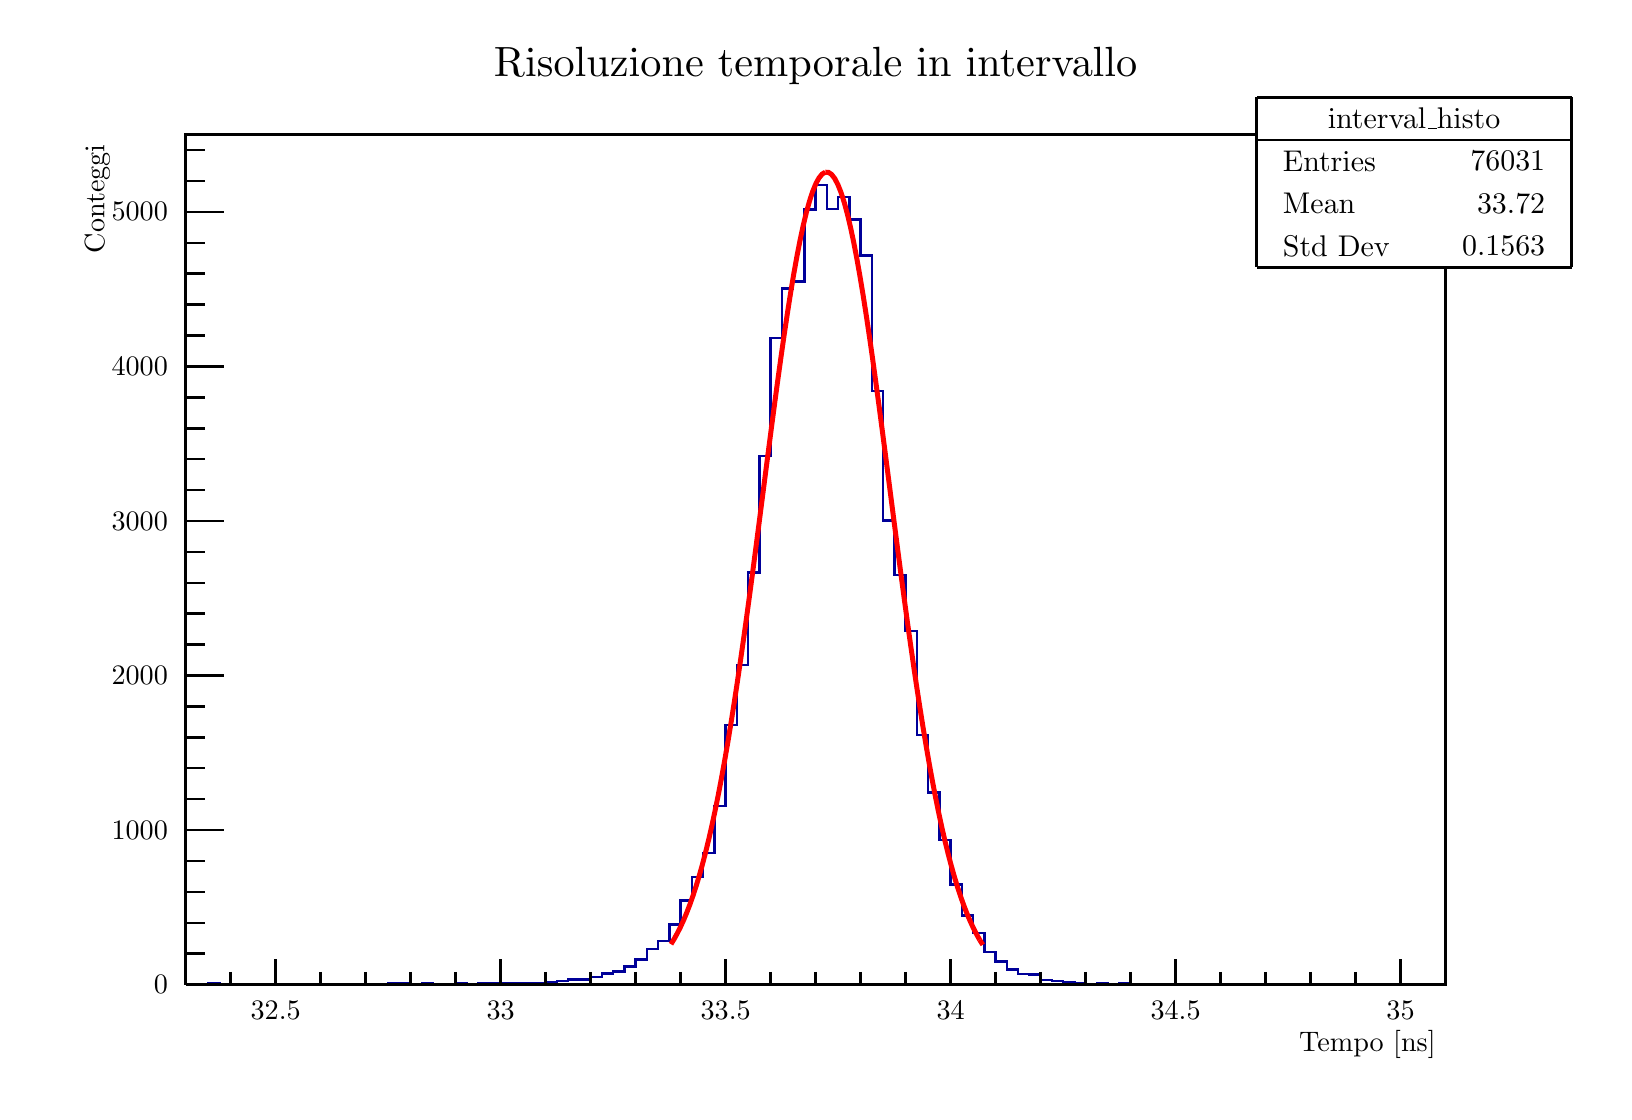
\begin{tikzpicture}
\pgfdeclareplotmark{cross} {
\pgfpathmoveto{\pgfpoint{-0.3\pgfplotmarksize}{\pgfplotmarksize}}
\pgfpathlineto{\pgfpoint{+0.3\pgfplotmarksize}{\pgfplotmarksize}}
\pgfpathlineto{\pgfpoint{+0.3\pgfplotmarksize}{0.3\pgfplotmarksize}}
\pgfpathlineto{\pgfpoint{+1\pgfplotmarksize}{0.3\pgfplotmarksize}}
\pgfpathlineto{\pgfpoint{+1\pgfplotmarksize}{-0.3\pgfplotmarksize}}
\pgfpathlineto{\pgfpoint{+0.3\pgfplotmarksize}{-0.3\pgfplotmarksize}}
\pgfpathlineto{\pgfpoint{+0.3\pgfplotmarksize}{-1.\pgfplotmarksize}}
\pgfpathlineto{\pgfpoint{-0.3\pgfplotmarksize}{-1.\pgfplotmarksize}}
\pgfpathlineto{\pgfpoint{-0.3\pgfplotmarksize}{-0.3\pgfplotmarksize}}
\pgfpathlineto{\pgfpoint{-1.\pgfplotmarksize}{-0.3\pgfplotmarksize}}
\pgfpathlineto{\pgfpoint{-1.\pgfplotmarksize}{0.3\pgfplotmarksize}}
\pgfpathlineto{\pgfpoint{-0.3\pgfplotmarksize}{0.3\pgfplotmarksize}}
\pgfpathclose
\pgfusepathqstroke
}
\pgfdeclareplotmark{cross*} {
\pgfpathmoveto{\pgfpoint{-0.3\pgfplotmarksize}{\pgfplotmarksize}}
\pgfpathlineto{\pgfpoint{+0.3\pgfplotmarksize}{\pgfplotmarksize}}
\pgfpathlineto{\pgfpoint{+0.3\pgfplotmarksize}{0.3\pgfplotmarksize}}
\pgfpathlineto{\pgfpoint{+1\pgfplotmarksize}{0.3\pgfplotmarksize}}
\pgfpathlineto{\pgfpoint{+1\pgfplotmarksize}{-0.3\pgfplotmarksize}}
\pgfpathlineto{\pgfpoint{+0.3\pgfplotmarksize}{-0.3\pgfplotmarksize}}
\pgfpathlineto{\pgfpoint{+0.3\pgfplotmarksize}{-1.\pgfplotmarksize}}
\pgfpathlineto{\pgfpoint{-0.3\pgfplotmarksize}{-1.\pgfplotmarksize}}
\pgfpathlineto{\pgfpoint{-0.3\pgfplotmarksize}{-0.3\pgfplotmarksize}}
\pgfpathlineto{\pgfpoint{-1.\pgfplotmarksize}{-0.3\pgfplotmarksize}}
\pgfpathlineto{\pgfpoint{-1.\pgfplotmarksize}{0.3\pgfplotmarksize}}
\pgfpathlineto{\pgfpoint{-0.3\pgfplotmarksize}{0.3\pgfplotmarksize}}
\pgfpathclose
\pgfusepathqfillstroke
}
\pgfdeclareplotmark{newstar} {
\pgfpathmoveto{\pgfqpoint{0pt}{\pgfplotmarksize}}
\pgfpathlineto{\pgfqpointpolar{44}{0.5\pgfplotmarksize}}
\pgfpathlineto{\pgfqpointpolar{18}{\pgfplotmarksize}}
\pgfpathlineto{\pgfqpointpolar{-20}{0.5\pgfplotmarksize}}
\pgfpathlineto{\pgfqpointpolar{-54}{\pgfplotmarksize}}
\pgfpathlineto{\pgfqpointpolar{-90}{0.5\pgfplotmarksize}}
\pgfpathlineto{\pgfqpointpolar{234}{\pgfplotmarksize}}
\pgfpathlineto{\pgfqpointpolar{198}{0.5\pgfplotmarksize}}
\pgfpathlineto{\pgfqpointpolar{162}{\pgfplotmarksize}}
\pgfpathlineto{\pgfqpointpolar{134}{0.5\pgfplotmarksize}}
\pgfpathclose
\pgfusepathqstroke
}
\pgfdeclareplotmark{newstar*} {
\pgfpathmoveto{\pgfqpoint{0pt}{\pgfplotmarksize}}
\pgfpathlineto{\pgfqpointpolar{44}{0.5\pgfplotmarksize}}
\pgfpathlineto{\pgfqpointpolar{18}{\pgfplotmarksize}}
\pgfpathlineto{\pgfqpointpolar{-20}{0.5\pgfplotmarksize}}
\pgfpathlineto{\pgfqpointpolar{-54}{\pgfplotmarksize}}
\pgfpathlineto{\pgfqpointpolar{-90}{0.5\pgfplotmarksize}}
\pgfpathlineto{\pgfqpointpolar{234}{\pgfplotmarksize}}
\pgfpathlineto{\pgfqpointpolar{198}{0.5\pgfplotmarksize}}
\pgfpathlineto{\pgfqpointpolar{162}{\pgfplotmarksize}}
\pgfpathlineto{\pgfqpointpolar{134}{0.5\pgfplotmarksize}}
\pgfpathclose
\pgfusepathqfillstroke
}
\definecolor{c}{rgb}{1,1,1};
\draw [color=c, fill=c] (0,0) rectangle (20,13.4957);
\draw [color=c, fill=c] (2,1.34957) rectangle (18,12.1461);
\definecolor{c}{rgb}{0,0,0};
\draw [c,line width=0.9] (2,1.34957) -- (2,12.1461) -- (18,12.1461) -- (18,1.34957) -- (2,1.34957);
\definecolor{c}{rgb}{1,1,1};
\draw [color=c, fill=c] (2,1.34957) rectangle (18,12.1461);
\definecolor{c}{rgb}{0,0,0};
\draw [c,line width=0.9] (2,1.34957) -- (2,12.1461) -- (18,12.1461) -- (18,1.34957) -- (2,1.34957);
\definecolor{c}{rgb}{0,0,0.6};
\draw [c,line width=0.9] (2,1.3535) -- (2.14286,1.3535) -- (2.14286,1.35742) -- (2.28571,1.35742) -- (2.28571,1.36723) -- (2.42857,1.36723) -- (2.42857,1.35742) -- (2.57143,1.35742) -- (2.57143,1.35546) -- (2.71429,1.35546) -- (2.71429,1.35938) --
 (2.85714,1.35938) -- (2.85714,1.35742) -- (3,1.35742) -- (3,1.35938) -- (3.14286,1.35938) -- (3.14286,1.35742) -- (3.28571,1.35742) -- (3.28571,1.35546) -- (3.42857,1.35546) -- (3.42857,1.35546) -- (3.57143,1.35546) -- (3.57143,1.35546) --
 (3.71429,1.35546) -- (3.71429,1.35153) -- (3.85714,1.35153) -- (3.85714,1.35153) -- (4,1.35153) -- (4,1.35742) -- (4.14286,1.35742) -- (4.14286,1.35938) -- (4.28571,1.35938) -- (4.28571,1.35153) -- (4.42857,1.35153) -- (4.42857,1.35546) --
 (4.57143,1.35546) -- (4.57143,1.37116) -- (4.71429,1.37116) -- (4.71429,1.36331) -- (4.85714,1.36331) -- (4.85714,1.35938) -- (5,1.35938) -- (5,1.36135) -- (5.14286,1.36135) -- (5.14286,1.35938) -- (5.28571,1.35938) -- (5.28571,1.35742) --
 (5.42857,1.35742) -- (5.42857,1.36527) -- (5.57143,1.36527) -- (5.57143,1.3535) -- (5.71429,1.3535) -- (5.71429,1.36135) -- (5.85714,1.36135) -- (5.85714,1.36331) -- (6,1.36331) -- (6,1.36723) -- (6.14286,1.36723) -- (6.14286,1.36331) --
 (6.28571,1.36331) -- (6.28571,1.36135) -- (6.42857,1.36135) -- (6.42857,1.3692) -- (6.57143,1.3692) -- (6.57143,1.38294) -- (6.71429,1.38294) -- (6.71429,1.39275) -- (6.85714,1.39275) -- (6.85714,1.4163) -- (7,1.4163) -- (7,1.4163) --
 (7.14286,1.4163) -- (7.14286,1.44574) -- (7.28571,1.44574) -- (7.28571,1.49285) -- (7.42857,1.49285) -- (7.42857,1.5164) -- (7.57143,1.5164) -- (7.57143,1.57724) -- (7.71429,1.57724) -- (7.71429,1.66949) -- (7.85714,1.66949) -- (7.85714,1.80099) --
 (8,1.80099) -- (8,1.90501) -- (8.14286,1.90501) -- (8.14286,2.11305) -- (8.28571,2.11305) -- (8.28571,2.41531) -- (8.42857,2.41531) -- (8.42857,2.71364) -- (8.57143,2.71364) -- (8.57143,3.01785) -- (8.71429,3.01785) -- (8.71429,3.6204) --
 (8.85714,3.6204) -- (8.85714,4.64492) -- (9,4.64492) -- (9,5.4084) -- (9.14286,5.4084) -- (9.14286,6.58601) -- (9.28571,6.58601) -- (9.28571,8.05999) -- (9.42857,8.05999) -- (9.42857,9.56144) -- (9.57143,9.56144) -- (9.57143,10.1915) --
 (9.71429,10.1915) -- (9.71429,10.2798) -- (9.85714,10.2798) -- (9.85714,11.1964) -- (10,11.1964) -- (10,11.5045) -- (10.1429,11.5045) -- (10.1429,11.2022) -- (10.2857,11.2022) -- (10.2857,11.3494) -- (10.4286,11.3494) -- (10.4286,11.0649) --
 (10.5714,11.0649) -- (10.5714,10.6095) -- (10.7143,10.6095) -- (10.7143,8.88628) -- (10.8571,8.88628) -- (10.8571,7.24155) -- (11,7.24155) -- (11,6.55264) -- (11.1429,6.55264) -- (11.1429,5.83823) -- (11.2857,5.83823) -- (11.2857,4.52127) --
 (11.4286,4.52127) -- (11.4286,3.78919) -- (11.5714,3.78919) -- (11.5714,3.18664) -- (11.7143,3.18664) -- (11.7143,2.62139) -- (11.8571,2.62139) -- (11.8571,2.22885) -- (12,2.22885) -- (12,2.00511) -- (12.1429,2.00511) -- (12.1429,1.7637) --
 (12.2857,1.7637) -- (12.2857,1.64005) -- (12.4286,1.64005) -- (12.4286,1.53995) -- (12.5714,1.53995) -- (12.5714,1.48303) -- (12.7143,1.48303) -- (12.7143,1.47518) -- (12.8571,1.47518) -- (12.8571,1.40649) -- (13,1.40649) -- (13,1.39864) --
 (13.1429,1.39864) -- (13.1429,1.37901) -- (13.2857,1.37901) -- (13.2857,1.3692) -- (13.4286,1.3692) -- (13.4286,1.35742) -- (13.5714,1.35742) -- (13.5714,1.36723) -- (13.7143,1.36723) -- (13.7143,1.35742) -- (13.8571,1.35742) -- (13.8571,1.36135) --
 (14,1.36135) -- (14,1.35546) -- (14.1429,1.35546) -- (14.1429,1.3535) -- (14.2857,1.3535) -- (14.2857,1.35153) -- (14.4286,1.35153) -- (14.4286,1.35938) -- (14.5714,1.35938) -- (14.5714,1.3535) -- (14.7143,1.3535) -- (14.7143,1.35153) --
 (14.8571,1.35153) -- (14.8571,1.34957) -- (15,1.34957) -- (15,1.3535) -- (15.1429,1.3535) -- (15.1429,1.35742) -- (15.2857,1.35742) -- (15.2857,1.35546) -- (15.4286,1.35546) -- (15.4286,1.34957) -- (15.5714,1.34957) -- (15.5714,1.35153) --
 (15.7143,1.35153) -- (15.7143,1.35153) -- (15.8571,1.35153) -- (15.8571,1.34957) -- (16,1.34957) -- (16,1.35153) -- (16.1429,1.35153) -- (16.1429,1.34957) -- (16.2857,1.34957) -- (16.2857,1.35153) -- (16.4286,1.35153) -- (16.4286,1.34957) --
 (16.5714,1.34957) -- (16.5714,1.34957) -- (16.7143,1.34957) -- (16.7143,1.34957) -- (16.8571,1.34957) -- (16.8571,1.35153) -- (17,1.35153) -- (17,1.35153) -- (17.1429,1.35153) -- (17.1429,1.34957) -- (17.2857,1.34957) -- (17.2857,1.35153) --
 (17.4286,1.35153) -- (17.4286,1.35153) -- (17.5714,1.35153) -- (17.5714,1.34957) -- (17.7143,1.34957) -- (17.7143,1.34957) -- (17.8571,1.34957) -- (17.8571,1.35153) -- (18,1.35153);
\definecolor{c}{rgb}{1,1,1};
\draw [color=c, fill=c] (15.6,10.4592) rectangle (19.6,12.6185);
\definecolor{c}{rgb}{0,0,0};
\draw [c,line width=0.9] (15.6,10.4592) -- (19.6,10.4592);
\draw [c,line width=0.9] (19.6,10.4592) -- (19.6,12.6185);
\draw [c,line width=0.9] (19.6,12.6185) -- (15.6,12.6185);
\draw [c,line width=0.9] (15.6,12.6185) -- (15.6,10.4592);
\draw (17.6,12.3486) node[scale=1.08185, color=c, rotate=0]{interval\_histo};
\draw [c,line width=0.9] (15.6,12.0787) -- (19.6,12.0787);
\draw [anchor= west] (15.8,11.8087) node[scale=1.08185, color=c, rotate=0]{Entries };
\draw [anchor= east] (19.4,11.8087) node[scale=1.08185, color=c, rotate=0]{ 76031};
\draw [anchor= west] (15.8,11.2689) node[scale=1.08185, color=c, rotate=0]{Mean  };
\draw [anchor= east] (19.4,11.2689) node[scale=1.08185, color=c, rotate=0]{  33.72};
\draw [anchor= west] (15.8,10.7291) node[scale=1.08185, color=c, rotate=0]{Std Dev   };
\draw [anchor= east] (19.4,10.7291) node[scale=1.08185, color=c, rotate=0]{ 0.1563};
\definecolor{c}{rgb}{1,0,0};
\draw [c,line width=1.8] (8.16286,1.86274) -- (8.20286,1.92828) -- (8.24286,2.00059) -- (8.28286,2.08014) -- (8.32286,2.16741) -- (8.36286,2.26284) -- (8.40286,2.36692) -- (8.44286,2.48007) -- (8.48286,2.60273) -- (8.52286,2.73528) --
 (8.56286,2.8781) -- (8.60286,3.0315) -- (8.64286,3.19575) -- (8.68286,3.37107) -- (8.72286,3.55762) -- (8.76286,3.75545) -- (8.80286,3.96459) -- (8.84286,4.18492) -- (8.88286,4.41628) -- (8.92286,4.65839) -- (8.96286,4.91084) -- (9.00286,5.17315) --
 (9.04286,5.44471) -- (9.08286,5.7248) -- (9.12286,6.01258) -- (9.16286,6.30709) -- (9.20286,6.60727) -- (9.24286,6.91195) -- (9.28286,7.21984) -- (9.32286,7.52958) -- (9.36286,7.83969) -- (9.40286,8.14865) -- (9.44286,8.45484) -- (9.48286,8.7566) --
 (9.52286,9.05223) -- (9.56286,9.34001) -- (9.60286,9.6182) -- (9.64286,9.88508) -- (9.68286,10.139) -- (9.72286,10.3782) -- (9.76286,10.6012) -- (9.80286,10.8064) -- (9.84286,10.9925) -- (9.88286,11.1581) -- (9.92286,11.3021) -- (9.96286,11.4234) --
 (10.0029,11.5211) -- (10.0429,11.5946) -- (10.0829,11.6434) -- (10.1229,11.667);
\draw [c,line width=1.8] (10.1229,11.667) -- (10.1629,11.6652) -- (10.2029,11.6382) -- (10.2429,11.5861) -- (10.2829,11.5092) -- (10.3229,11.4082) -- (10.3629,11.2837) -- (10.4029,11.1368) -- (10.4429,10.9683) -- (10.4829,10.7795) --
 (10.5229,10.5718) -- (10.5629,10.3465) -- (10.6029,10.1052) -- (10.6429,9.84943) -- (10.6829,9.5809) -- (10.7229,9.3013) -- (10.7629,9.01235) -- (10.8029,8.71578) -- (10.8429,8.41332) -- (10.8829,8.10665) -- (10.9229,7.79745) -- (10.9629,7.48729) --
 (11.0029,7.17772) -- (11.0429,6.87019) -- (11.0829,6.56605) -- (11.1229,6.26658) -- (11.1629,5.97292) -- (11.2029,5.68614) -- (11.2429,5.40717) -- (11.2829,5.13683) -- (11.3229,4.87583) -- (11.3629,4.62476) -- (11.4029,4.3841) -- (11.4429,4.15423)
 -- (11.4829,3.93541) -- (11.5229,3.72781) -- (11.5629,3.53152) -- (11.6029,3.34651) -- (11.6429,3.17271) -- (11.6829,3.00995) -- (11.7229,2.85801) -- (11.7629,2.71661) -- (11.8029,2.58543) -- (11.8429,2.46409) -- (11.8829,2.3522) --
 (11.9229,2.24933) -- (11.9629,2.15504) -- (12.0029,2.06885) -- (12.0429,1.99032) -- (12.0829,1.91895);
\draw [c,line width=1.8] (12.0829,1.91895) -- (12.1229,1.8543);
\definecolor{c}{rgb}{0,0,0};
\draw [c,line width=0.9] (2,1.34957) -- (18,1.34957);
\draw [anchor= east] (18,0.593811) node[scale=1.01821, color=c, rotate=0]{Tempo [ns]};
\draw [c,line width=0.9] (3.14286,1.67347) -- (3.14286,1.34957);
\draw [c,line width=0.9] (3.71429,1.51152) -- (3.71429,1.34957);
\draw [c,line width=0.9] (4.28571,1.51152) -- (4.28571,1.34957);
\draw [c,line width=0.9] (4.85714,1.51152) -- (4.85714,1.34957);
\draw [c,line width=0.9] (5.42857,1.51152) -- (5.42857,1.34957);
\draw [c,line width=0.9] (6,1.67347) -- (6,1.34957);
\draw [c,line width=0.9] (6.57143,1.51152) -- (6.57143,1.34957);
\draw [c,line width=0.9] (7.14286,1.51152) -- (7.14286,1.34957);
\draw [c,line width=0.9] (7.71429,1.51152) -- (7.71429,1.34957);
\draw [c,line width=0.9] (8.28571,1.51152) -- (8.28571,1.34957);
\draw [c,line width=0.9] (8.85714,1.67347) -- (8.85714,1.34957);
\draw [c,line width=0.9] (9.42857,1.51152) -- (9.42857,1.34957);
\draw [c,line width=0.9] (10,1.51152) -- (10,1.34957);
\draw [c,line width=0.9] (10.5714,1.51152) -- (10.5714,1.34957);
\draw [c,line width=0.9] (11.1429,1.51152) -- (11.1429,1.34957);
\draw [c,line width=0.9] (11.7143,1.67347) -- (11.7143,1.34957);
\draw [c,line width=0.9] (12.2857,1.51152) -- (12.2857,1.34957);
\draw [c,line width=0.9] (12.8571,1.51152) -- (12.8571,1.34957);
\draw [c,line width=0.9] (13.4286,1.51152) -- (13.4286,1.34957);
\draw [c,line width=0.9] (14,1.51152) -- (14,1.34957);
\draw [c,line width=0.9] (14.5714,1.67347) -- (14.5714,1.34957);
\draw [c,line width=0.9] (15.1429,1.51152) -- (15.1429,1.34957);
\draw [c,line width=0.9] (15.7143,1.51152) -- (15.7143,1.34957);
\draw [c,line width=0.9] (16.2857,1.51152) -- (16.2857,1.34957);
\draw [c,line width=0.9] (16.8571,1.51152) -- (16.8571,1.34957);
\draw [c,line width=0.9] (17.4286,1.67347) -- (17.4286,1.34957);
\draw [c,line width=0.9] (3.14286,1.67347) -- (3.14286,1.34957);
\draw [c,line width=0.9] (2.57143,1.51152) -- (2.57143,1.34957);
\draw [c,line width=0.9] (2,1.51152) -- (2,1.34957);
\draw [c,line width=0.9] (17.4286,1.67347) -- (17.4286,1.34957);
\draw [c,line width=0.9] (18,1.51152) -- (18,1.34957);
\draw [anchor=base] (3.14286,0.904212) node[scale=1.01821, color=c, rotate=0]{32.5};
\draw [anchor=base] (6,0.904212) node[scale=1.01821, color=c, rotate=0]{33};
\draw [anchor=base] (8.85714,0.904212) node[scale=1.01821, color=c, rotate=0]{33.5};
\draw [anchor=base] (11.7143,0.904212) node[scale=1.01821, color=c, rotate=0]{34};
\draw [anchor=base] (14.5714,0.904212) node[scale=1.01821, color=c, rotate=0]{34.5};
\draw [anchor=base] (17.4286,0.904212) node[scale=1.01821, color=c, rotate=0]{35};
\draw [c,line width=0.9] (2,1.34957) -- (2,12.1461);
\draw [anchor= east] (0.88,12.1461) node[scale=1.01821, color=c, rotate=90]{Conteggi};
\draw [c,line width=0.9] (2.48,1.34957) -- (2,1.34957);
\draw [c,line width=0.9] (2.24,1.74211) -- (2,1.74211);
\draw [c,line width=0.9] (2.24,2.13464) -- (2,2.13464);
\draw [c,line width=0.9] (2.24,2.52718) -- (2,2.52718);
\draw [c,line width=0.9] (2.24,2.91972) -- (2,2.91972);
\draw [c,line width=0.9] (2.48,3.31225) -- (2,3.31225);
\draw [c,line width=0.9] (2.24,3.70479) -- (2,3.70479);
\draw [c,line width=0.9] (2.24,4.09733) -- (2,4.09733);
\draw [c,line width=0.9] (2.24,4.48986) -- (2,4.48986);
\draw [c,line width=0.9] (2.24,4.8824) -- (2,4.8824);
\draw [c,line width=0.9] (2.48,5.27494) -- (2,5.27494);
\draw [c,line width=0.9] (2.24,5.66747) -- (2,5.66747);
\draw [c,line width=0.9] (2.24,6.06001) -- (2,6.06001);
\draw [c,line width=0.9] (2.24,6.45255) -- (2,6.45255);
\draw [c,line width=0.9] (2.24,6.84508) -- (2,6.84508);
\draw [c,line width=0.9] (2.48,7.23762) -- (2,7.23762);
\draw [c,line width=0.9] (2.24,7.63016) -- (2,7.63016);
\draw [c,line width=0.9] (2.24,8.02269) -- (2,8.02269);
\draw [c,line width=0.9] (2.24,8.41523) -- (2,8.41523);
\draw [c,line width=0.9] (2.24,8.80777) -- (2,8.80777);
\draw [c,line width=0.9] (2.48,9.2003) -- (2,9.2003);
\draw [c,line width=0.9] (2.24,9.59284) -- (2,9.59284);
\draw [c,line width=0.9] (2.24,9.98538) -- (2,9.98538);
\draw [c,line width=0.9] (2.24,10.3779) -- (2,10.3779);
\draw [c,line width=0.9] (2.24,10.7705) -- (2,10.7705);
\draw [c,line width=0.9] (2.48,11.163) -- (2,11.163);
\draw [c,line width=0.9] (2.48,11.163) -- (2,11.163);
\draw [c,line width=0.9] (2.24,11.5555) -- (2,11.5555);
\draw [c,line width=0.9] (2.24,11.9481) -- (2,11.9481);
\draw [anchor= east] (1.9,1.34957) node[scale=1.01821, color=c, rotate=0]{0};
\draw [anchor= east] (1.9,3.31225) node[scale=1.01821, color=c, rotate=0]{1000};
\draw [anchor= east] (1.9,5.27494) node[scale=1.01821, color=c, rotate=0]{2000};
\draw [anchor= east] (1.9,7.23762) node[scale=1.01821, color=c, rotate=0]{3000};
\draw [anchor= east] (1.9,9.2003) node[scale=1.01821, color=c, rotate=0]{4000};
\draw [anchor= east] (1.9,11.163) node[scale=1.01821, color=c, rotate=0]{5000};
\definecolor{c}{rgb}{1,1,1};
\draw [color=c, fill=c] (15.6,10.4592) rectangle (19.6,12.6185);
\definecolor{c}{rgb}{0,0,0};
\draw [c,line width=0.9] (15.6,10.4592) -- (19.6,10.4592);
\draw [c,line width=0.9] (19.6,10.4592) -- (19.6,12.6185);
\draw [c,line width=0.9] (19.6,12.6185) -- (15.6,12.6185);
\draw [c,line width=0.9] (15.6,12.6185) -- (15.6,10.4592);
\draw (17.6,12.3486) node[scale=1.08185, color=c, rotate=0]{interval\_histo};
\draw [c,line width=0.9] (15.6,12.0787) -- (19.6,12.0787);
\draw [anchor= west] (15.8,11.8087) node[scale=1.08185, color=c, rotate=0]{Entries };
\draw [anchor= east] (19.4,11.8087) node[scale=1.08185, color=c, rotate=0]{ 76031};
\draw [anchor= west] (15.8,11.2689) node[scale=1.08185, color=c, rotate=0]{Mean  };
\draw [anchor= east] (19.4,11.2689) node[scale=1.08185, color=c, rotate=0]{  33.72};
\draw [anchor= west] (15.8,10.7291) node[scale=1.08185, color=c, rotate=0]{Std Dev   };
\draw [anchor= east] (19.4,10.7291) node[scale=1.08185, color=c, rotate=0]{ 0.1563};
\draw (10,13.0156) node[scale=1.52731, color=c, rotate=0]{Risoluzione temporale in intervallo};
\end{tikzpicture}
